\documentclass[twoside]{book}

% Packages required by doxygen
\usepackage{fixltx2e}
\usepackage{calc}
\usepackage{doxygen}
\usepackage[export]{adjustbox} % also loads graphicx
\usepackage{graphicx}
\usepackage[utf8]{inputenc}
\usepackage{makeidx}
\usepackage{multicol}
\usepackage{multirow}
\PassOptionsToPackage{warn}{textcomp}
\usepackage{textcomp}
\usepackage[nointegrals]{wasysym}
\usepackage[table]{xcolor}

% Font selection
\usepackage[T1]{fontenc}
\usepackage[scaled=.90]{helvet}
\usepackage{courier}
\usepackage{amssymb}
\usepackage{sectsty}
\renewcommand{\familydefault}{\sfdefault}
\allsectionsfont{%
  \fontseries{bc}\selectfont%
  \color{darkgray}%
}
\renewcommand{\DoxyLabelFont}{%
  \fontseries{bc}\selectfont%
  \color{darkgray}%
}
\newcommand{\+}{\discretionary{\mbox{\scriptsize$\hookleftarrow$}}{}{}}

% Page & text layout
\usepackage{geometry}
\geometry{%
  a4paper,%
  top=2.5cm,%
  bottom=2.5cm,%
  left=2.5cm,%
  right=2.5cm%
}
\tolerance=750
\hfuzz=15pt
\hbadness=750
\setlength{\emergencystretch}{15pt}
\setlength{\parindent}{0cm}
\setlength{\parskip}{3ex plus 2ex minus 2ex}
\makeatletter
\renewcommand{\paragraph}{%
  \@startsection{paragraph}{4}{0ex}{-1.0ex}{1.0ex}{%
    \normalfont\normalsize\bfseries\SS@parafont%
  }%
}
\renewcommand{\subparagraph}{%
  \@startsection{subparagraph}{5}{0ex}{-1.0ex}{1.0ex}{%
    \normalfont\normalsize\bfseries\SS@subparafont%
  }%
}
\makeatother

% Headers & footers
\usepackage{fancyhdr}
\pagestyle{fancyplain}
\fancyhead[LE]{\fancyplain{}{\bfseries\thepage}}
\fancyhead[CE]{\fancyplain{}{}}
\fancyhead[RE]{\fancyplain{}{\bfseries\leftmark}}
\fancyhead[LO]{\fancyplain{}{\bfseries\rightmark}}
\fancyhead[CO]{\fancyplain{}{}}
\fancyhead[RO]{\fancyplain{}{\bfseries\thepage}}
\fancyfoot[LE]{\fancyplain{}{}}
\fancyfoot[CE]{\fancyplain{}{}}
\fancyfoot[RE]{\fancyplain{}{\bfseries\scriptsize Generated by Doxygen }}
\fancyfoot[LO]{\fancyplain{}{\bfseries\scriptsize Generated by Doxygen }}
\fancyfoot[CO]{\fancyplain{}{}}
\fancyfoot[RO]{\fancyplain{}{}}
\renewcommand{\footrulewidth}{0.4pt}
\renewcommand{\chaptermark}[1]{%
  \markboth{#1}{}%
}
\renewcommand{\sectionmark}[1]{%
  \markright{\thesection\ #1}%
}

% Indices & bibliography
\usepackage{natbib}
\usepackage[titles]{tocloft}
\setcounter{tocdepth}{3}
\setcounter{secnumdepth}{5}
\makeindex

% Hyperlinks (required, but should be loaded last)
\usepackage{ifpdf}
\ifpdf
  \usepackage[pdftex,pagebackref=true]{hyperref}
\else
  \usepackage[ps2pdf,pagebackref=true]{hyperref}
\fi
\hypersetup{%
  colorlinks=true,%
  linkcolor=blue,%
  citecolor=blue,%
  unicode%
}

% Custom commands
\newcommand{\clearemptydoublepage}{%
  \newpage{\pagestyle{empty}\cleardoublepage}%
}

\usepackage{caption}
\captionsetup{labelsep=space,justification=centering,font={bf},singlelinecheck=off,skip=4pt,position=top}

%===== C O N T E N T S =====

\begin{document}

% Titlepage & ToC
\hypersetup{pageanchor=false,
             bookmarksnumbered=true,
             pdfencoding=unicode
            }
\pagenumbering{alph}
\begin{titlepage}
\vspace*{7cm}
\begin{center}%
{\Large E\+C\+E1186 }\\
\vspace*{1cm}
{\large Generated by Doxygen 1.8.13}\\
\end{center}
\end{titlepage}
\clearemptydoublepage
\pagenumbering{roman}
\tableofcontents
\clearemptydoublepage
\pagenumbering{arabic}
\hypersetup{pageanchor=true}

%--- Begin generated contents ---
\chapter{Todo List}
\label{todo}
\Hypertarget{todo}

\begin{DoxyRefList}
\item[\label{todo__todo000001}%
\Hypertarget{todo__todo000001}%
Member \hyperlink{classTrackModel_1_1Block_ade3dc0b39ce6d111e7491443b052051e}{Track\+Model.Block.set\+Light\+State} (Integer set\+Int)]Add strict value assertions that set\+Int is either 0 or 1  
\item[\label{todo__todo000002}%
\Hypertarget{todo__todo000002}%
Member \hyperlink{classTrackModel_1_1Block_aa206833e61700249e5905fe6e6126399}{Track\+Model.Block.set\+Switch\+State} (Integer set\+Int)]Add strict value assertions that set\+Int is either 0 or 1 
\end{DoxyRefList}
\chapter{Bug List}
\label{bug}
\Hypertarget{bug}

\begin{DoxyRefList}
\item[\label{bug__bug000001}%
\Hypertarget{bug__bug000001}%
Member \hyperlink{classTrackModel_1_1TrackGUI_aa7c85f553a7540a8f20b2092d8a6ca8a}{Track\+Model.Track\+G\+UI.action\+Performed} (Action\+Event e)]The segment and block descriptors need to be cleared when selecting a dropdown from line. In its current configuration, it will not reset to empty fields, allowing the user to select blocks that do not exist. This condition applies to selecting a new line while holding segment and block constant.

It is possible for a user to select default vaules in the dropdown menu. When selecting the default values, it results in an unhandled exception, rendering the program unusable. 
\end{DoxyRefList}
\chapter{Namespace Index}
\section{Packages}
Here are the packages with brief descriptions (if available)\+:\begin{DoxyCompactList}
\item\contentsline{section}{\hyperlink{namespaceCommonUIElements}{Common\+U\+I\+Elements} }{\pageref{namespaceCommonUIElements}}{}
\item\contentsline{section}{\hyperlink{namespaceTrackModel}{Track\+Model} \\*G\+UI associated with the track module }{\pageref{namespaceTrackModel}}{}
\item\contentsline{section}{\hyperlink{namespaceTrackModelTest}{Track\+Model\+Test} }{\pageref{namespaceTrackModelTest}}{}
\item\contentsline{section}{\hyperlink{namespaceTrainControllerComps}{Train\+Controller\+Comps} }{\pageref{namespaceTrainControllerComps}}{}
\item\contentsline{section}{\hyperlink{namespacetrainModel}{train\+Model} }{\pageref{namespacetrainModel}}{}
\item\contentsline{section}{\hyperlink{namespaceWaysideController}{Wayside\+Controller} }{\pageref{namespaceWaysideController}}{}
\end{DoxyCompactList}

\chapter{Hierarchical Index}
\section{Class Hierarchy}
This inheritance list is sorted roughly, but not completely, alphabetically\+:\begin{DoxyCompactList}
\item Array\+List$<$ track\+Details $>$\item Array\+List$<$ Track\+Model.\+Block $>$\item Array\+List$<$ train $>$\item Array\+List$<$ Wayside\+Controller.\+WS $>$\item Comparable\begin{DoxyCompactList}
\item \contentsline{section}{Track\+Model.\+Block}{\pageref{classTrackModel_1_1Block}}{}
\item \contentsline{section}{Track\+Model.\+Station}{\pageref{classTrackModel_1_1Station}}{}
\end{DoxyCompactList}
\item \contentsline{section}{Track\+Model\+Test.\+Comparable\+Test}{\pageref{classTrackModelTest_1_1ComparableTest}}{}
\item \contentsline{section}{Track\+Model.\+Crossing}{\pageref{classTrackModel_1_1Crossing}}{}
\item \contentsline{section}{C\+T\+C\+\_\+gui}{\pageref{classCTC__gui}}{}
\item \contentsline{section}{dispatch\+Train\+Popup}{\pageref{classdispatchTrainPopup}}{}
\item \contentsline{section}{Track\+Model\+Test.\+Greenline\+Test}{\pageref{classTrackModelTest_1_1GreenlineTest}}{}
\item Hash\+Map$<$ String, Array\+List$<$ Track\+Model.\+Block $>$ $>$\item Hash\+Map$<$ String, Hash\+Map$<$ String, Hash\+Map$<$ Integer, Track\+Model.\+Block $>$ $>$ $>$\item Hash\+Map$<$ String, Track\+Model.\+Block $>$\item Hash\+Map$<$ String, Track\+Model.\+Station $>$\item Hash\+Map$<$ String, Train\+Controller\+Comps.\+Test\+Train $>$\item Hash\+Map$<$ Track\+Model.\+Block, Track\+Model.\+Crossing $>$\item Hash\+Map$<$ Track\+Model.\+Block, Track\+Model.\+Station $>$\item J\+Combo\+Box$<$ String $>$\item J\+Frame\begin{DoxyCompactList}
\item \contentsline{section}{Common\+U\+I\+Elements.\+Confirmation\+Window}{\pageref{classCommonUIElements_1_1ConfirmationWindow}}{}
\item \contentsline{section}{Train\+Controller\+Comps.\+T\+C\+Dispatched\+Train\+Frame}{\pageref{classTrainControllerComps_1_1TCDispatchedTrainFrame}}{}
\item \contentsline{section}{Train\+Controller\+Comps.\+T\+C\+Emergency\+Frame}{\pageref{classTrainControllerComps_1_1TCEmergencyFrame}}{}
\item \contentsline{section}{Train\+Controller\+Comps.\+T\+C\+Engineer\+Panel}{\pageref{classTrainControllerComps_1_1TCEngineerPanel}}{}
\item \contentsline{section}{Train\+Controller\+Comps.\+T\+C\+Failures}{\pageref{classTrainControllerComps_1_1TCFailures}}{}
\item \contentsline{section}{Train\+Controller\+Comps.\+T\+C\+Passenger\+G\+UI}{\pageref{classTrainControllerComps_1_1TCPassengerGUI}}{}
\item \contentsline{section}{Train\+Controller\+Comps.\+T\+C\+Test\+Console}{\pageref{classTrainControllerComps_1_1TCTestConsole}}{}
\item \contentsline{section}{Train\+Controller\+Comps.\+Train\+Controller}{\pageref{classTrainControllerComps_1_1TrainController}}{}
\end{DoxyCompactList}
\item J\+Panel\begin{DoxyCompactList}
\item \contentsline{section}{Train\+Controller\+Comps.\+T\+C\+Block\+Info\+Panel}{\pageref{classTrainControllerComps_1_1TCBlockInfoPanel}}{}
\item \contentsline{section}{Train\+Controller\+Comps.\+T\+C\+Brake\+Panel}{\pageref{classTrainControllerComps_1_1TCBrakePanel}}{}
\item \contentsline{section}{Train\+Controller\+Comps.\+T\+C\+Speed\+Controller}{\pageref{classTrainControllerComps_1_1TCSpeedController}}{}
\item \contentsline{section}{Train\+Controller\+Comps.\+T\+C\+Train\+Info\+Pane}{\pageref{classTrainControllerComps_1_1TCTrainInfoPane}}{}
\item \contentsline{section}{Train\+Controller\+Comps.\+T\+C\+Utility\+Panel}{\pageref{classTrainControllerComps_1_1TCUtilityPanel}}{}
\end{DoxyCompactList}
\item \contentsline{section}{launch}{\pageref{classlaunch}}{}
\item \contentsline{section}{train\+Model.\+Launch}{\pageref{classtrainModel_1_1Launch}}{}
\item \contentsline{section}{Launcher}{\pageref{classLauncher}}{}
\item Linked\+List$<$ String $>$\item Linked\+List$<$ Train\+Controller\+Comps.\+Test\+Train $>$\item \contentsline{section}{Wayside\+Controller.\+P\+LC}{\pageref{classWaysideController_1_1PLC}}{}
\item \contentsline{section}{Track\+Model\+Test.\+Redline\+Test}{\pageref{classTrackModelTest_1_1RedlineTest}}{}
\item \contentsline{section}{train\+Model.\+tester}{\pageref{classtrainModel_1_1tester}}{}
\item \contentsline{section}{Wayside\+Controller.\+test\+Pop\+Up}{\pageref{classWaysideController_1_1testPopUp}}{}
\item \contentsline{section}{Train\+Controller\+Comps.\+Test\+Train}{\pageref{classTrainControllerComps_1_1TestTrain}}{}
\item \contentsline{section}{track\+Details}{\pageref{classtrackDetails}}{}
\item \contentsline{section}{Track\+Model.\+Track\+G\+UI}{\pageref{classTrackModel_1_1TrackGUI}}{}
\item \contentsline{section}{Track\+Model.\+Track\+Model}{\pageref{classTrackModel_1_1TrackModel}}{}
\item \contentsline{section}{train\+Model.\+Train}{\pageref{classtrainModel_1_1Train}}{}
\item \contentsline{section}{train}{\pageref{classtrain}}{}
\item \contentsline{section}{train\+Model.\+train\+Mode\+UI}{\pageref{classtrainModel_1_1trainModeUI}}{}
\item Tree\+Set$<$ Integer $>$\item Tree\+Set$<$ String $>$\item \contentsline{section}{Wayside\+Controller.\+Wayside\+Gui\+Main}{\pageref{classWaysideController_1_1WaysideGuiMain}}{}
\item \contentsline{section}{Wayside\+Controller.\+Wayside\+P\+LC}{\pageref{classWaysideController_1_1WaysidePLC}}{}
\item Action\+Event\item Action\+Listener\item After\+Each\item Array\+List\item Arrays\item Attribute\+Set\item Before\+Each\item Border\item Box\item Buffered\+Reader\item Button\+Group\item Calendar\item Change\+Event\item Change\+Listener\item Charset\item Choice\item Collections\item Color\item Component\item Date\+Format\item Date\+Time\+Formatter\item Default\+Combo\+Box\+Model\item Display\+Name\item D\+I\+S\+P\+O\+S\+E\+\_\+\+O\+N\+\_\+\+C\+L\+O\+SE\item Event\+Queue\item File\+Input\+Stream\item File\+Name\+Extension\+Filter\item File\+Not\+Found\+Exception\item File\+Reader\item Font\item Hash\+Map\item Input\+Stream\+Reader\item I\+O\+Exception\item Item\+Event\item Iterator\item J\+Button\item J\+Combo\+Box\item J\+Frame\item J\+Label\item J\+Menu\item J\+Menu\+Bar\item J\+Menu\+Item\item J\+Panel\begin{DoxyCompactList}
\item \contentsline{section}{Wayside\+Controller.\+WS}{\pageref{classWaysideController_1_1WS}}{}
\end{DoxyCompactList}
\item J\+Radio\+Button\item J\+Separator\item J\+Slider\item J\+Text\+Area\item J\+Text\+Field\item J\+Text\+Pane\item J\+Toggle\+Button\item J\+Tool\+Bar\item Linked\+List\item List\item List\+Model\item Local\+Date\item Number\+Format\+Exception\item Properties\item Random\item Scanner\item Script\+Exception\item Set\item Simple\+Attribute\+Set\item Simple\+Date\+Format\item Style\+Constants\item Style\+Context\item Swing\+Constants\item System\+Color\item Test\item Timer\item Tree\+Set\item Unsupported\+Look\+And\+Feel\+Exception\end{DoxyCompactList}

\chapter{Class Index}
\section{Class List}
Here are the classes, structs, unions and interfaces with brief descriptions\+:\begin{DoxyCompactList}
\item\contentsline{section}{\hyperlink{classTrackModel_1_1Block}{Track\+Model.\+Block} }{\pageref{classTrackModel_1_1Block}}{}
\item\contentsline{section}{\hyperlink{classTrackModelTest_1_1ComparableTest}{Track\+Model\+Test.\+Comparable\+Test} }{\pageref{classTrackModelTest_1_1ComparableTest}}{}
\item\contentsline{section}{\hyperlink{classCommonUIElements_1_1ConfirmationWindow}{Common\+U\+I\+Elements.\+Confirmation\+Window} \\*A window that displays a title and a message for a given amount of time, in seconds, and then closes }{\pageref{classCommonUIElements_1_1ConfirmationWindow}}{}
\item\contentsline{section}{\hyperlink{classTrackModel_1_1Crossing}{Track\+Model.\+Crossing} }{\pageref{classTrackModel_1_1Crossing}}{}
\item\contentsline{section}{\hyperlink{classCTC__gui}{C\+T\+C\+\_\+gui} }{\pageref{classCTC__gui}}{}
\item\contentsline{section}{\hyperlink{classdispatchTrainPopup}{dispatch\+Train\+Popup} }{\pageref{classdispatchTrainPopup}}{}
\item\contentsline{section}{\hyperlink{classTrackModelTest_1_1GreenlineTest}{Track\+Model\+Test.\+Greenline\+Test} }{\pageref{classTrackModelTest_1_1GreenlineTest}}{}
\item\contentsline{section}{\hyperlink{classlaunch}{launch} }{\pageref{classlaunch}}{}
\item\contentsline{section}{\hyperlink{classtrainModel_1_1Launch}{train\+Model.\+Launch} }{\pageref{classtrainModel_1_1Launch}}{}
\item\contentsline{section}{\hyperlink{classLauncher}{Launcher} }{\pageref{classLauncher}}{}
\item\contentsline{section}{\hyperlink{classWaysideController_1_1PLC}{Wayside\+Controller.\+P\+LC} }{\pageref{classWaysideController_1_1PLC}}{}
\item\contentsline{section}{\hyperlink{classTrackModelTest_1_1RedlineTest}{Track\+Model\+Test.\+Redline\+Test} }{\pageref{classTrackModelTest_1_1RedlineTest}}{}
\item\contentsline{section}{\hyperlink{classTrackModel_1_1Station}{Track\+Model.\+Station} }{\pageref{classTrackModel_1_1Station}}{}
\item\contentsline{section}{\hyperlink{classTrainControllerComps_1_1TCBlockInfoPanel}{Train\+Controller\+Comps.\+T\+C\+Block\+Info\+Panel} \\*This class is responsible for displaying information regarding the block the selected train is currently in }{\pageref{classTrainControllerComps_1_1TCBlockInfoPanel}}{}
\item\contentsline{section}{\hyperlink{classTrainControllerComps_1_1TCBrakePanel}{Train\+Controller\+Comps.\+T\+C\+Brake\+Panel} \\*This class is responsible for applying and managing the use of a train\textquotesingle{}s braking system }{\pageref{classTrainControllerComps_1_1TCBrakePanel}}{}
\item\contentsline{section}{\hyperlink{classTrainControllerComps_1_1TCDispatchedTrainFrame}{Train\+Controller\+Comps.\+T\+C\+Dispatched\+Train\+Frame} \\*This class is responsible for displaying all the dispatched trains to the user, and allow them to open multiple Train Controllers for selected trains }{\pageref{classTrainControllerComps_1_1TCDispatchedTrainFrame}}{}
\item\contentsline{section}{\hyperlink{classTrainControllerComps_1_1TCEmergencyFrame}{Train\+Controller\+Comps.\+T\+C\+Emergency\+Frame} \\*This class is responsible for confirming the use of the selected trains emergency brake when in Manual mode }{\pageref{classTrainControllerComps_1_1TCEmergencyFrame}}{}
\item\contentsline{section}{\hyperlink{classTrainControllerComps_1_1TCEngineerPanel}{Train\+Controller\+Comps.\+T\+C\+Engineer\+Panel} \\*This class is responsible to set the Kp and Ki constants of a given train }{\pageref{classTrainControllerComps_1_1TCEngineerPanel}}{}
\item\contentsline{section}{\hyperlink{classTrainControllerComps_1_1TCFailures}{Train\+Controller\+Comps.\+T\+C\+Failures} \\*This class is responsible for display the states of the 3 failures that can occur on the train, as well as sending a signal to the C\+TC to repair the broken systems }{\pageref{classTrainControllerComps_1_1TCFailures}}{}
\item\contentsline{section}{\hyperlink{classTrainControllerComps_1_1TCPassengerGUI}{Train\+Controller\+Comps.\+T\+C\+Passenger\+G\+UI} \\*This class is responsible for allowing the passengers on the train to initiate the emergency brake on a selected train }{\pageref{classTrainControllerComps_1_1TCPassengerGUI}}{}
\item\contentsline{section}{\hyperlink{classTrainControllerComps_1_1TCSpeedController}{Train\+Controller\+Comps.\+T\+C\+Speed\+Controller} \\*This class is responsible for allowing the user to set the speed of the selected train if in Manual mode, or controls the speed automatically if in Automatic mode }{\pageref{classTrainControllerComps_1_1TCSpeedController}}{}
\item\contentsline{section}{\hyperlink{classTrainControllerComps_1_1TCTestConsole}{Train\+Controller\+Comps.\+T\+C\+Test\+Console} \\*This class is responsible for testing the various components in the Train Controller, mimicking the components on a train object }{\pageref{classTrainControllerComps_1_1TCTestConsole}}{}
\item\contentsline{section}{\hyperlink{classTrainControllerComps_1_1TCTrainInfoPane}{Train\+Controller\+Comps.\+T\+C\+Train\+Info\+Pane} \\*A component of the Train Controller responsible for the selected train\textquotesingle{}s speed, power, authority, and suggested speed }{\pageref{classTrainControllerComps_1_1TCTrainInfoPane}}{}
\item\contentsline{section}{\hyperlink{classTrainControllerComps_1_1TCUtilityPanel}{Train\+Controller\+Comps.\+T\+C\+Utility\+Panel} \\*A component of the Train Controller responsible for displaying, and transmitting information and changes to the train corresponding to the Air Conditioning unit (AC), Heating unit, Left/\+Right Doors, and Lights }{\pageref{classTrainControllerComps_1_1TCUtilityPanel}}{}
\item\contentsline{section}{\hyperlink{classtrainModel_1_1tester}{train\+Model.\+tester} }{\pageref{classtrainModel_1_1tester}}{}
\item\contentsline{section}{\hyperlink{classWaysideController_1_1testPopUp}{Wayside\+Controller.\+test\+Pop\+Up} }{\pageref{classWaysideController_1_1testPopUp}}{}
\item\contentsline{section}{\hyperlink{classTrainControllerComps_1_1TestTrain}{Train\+Controller\+Comps.\+Test\+Train} }{\pageref{classTrainControllerComps_1_1TestTrain}}{}
\item\contentsline{section}{\hyperlink{classtrackDetails}{track\+Details} }{\pageref{classtrackDetails}}{}
\item\contentsline{section}{\hyperlink{classTrackModel_1_1TrackGUI}{Track\+Model.\+Track\+G\+UI} }{\pageref{classTrackModel_1_1TrackGUI}}{}
\item\contentsline{section}{\hyperlink{classTrackModel_1_1TrackModel}{Track\+Model.\+Track\+Model} }{\pageref{classTrackModel_1_1TrackModel}}{}
\item\contentsline{section}{\hyperlink{classtrainModel_1_1Train}{train\+Model.\+Train} }{\pageref{classtrainModel_1_1Train}}{}
\item\contentsline{section}{\hyperlink{classtrain}{train} }{\pageref{classtrain}}{}
\item\contentsline{section}{\hyperlink{classTrainControllerComps_1_1TrainController}{Train\+Controller\+Comps.\+Train\+Controller} \\*This class is a G\+UI that is used to control a selected train }{\pageref{classTrainControllerComps_1_1TrainController}}{}
\item\contentsline{section}{\hyperlink{classtrainModel_1_1trainModeUI}{train\+Model.\+train\+Mode\+UI} }{\pageref{classtrainModel_1_1trainModeUI}}{}
\item\contentsline{section}{\hyperlink{classWaysideController_1_1WaysideGuiMain}{Wayside\+Controller.\+Wayside\+Gui\+Main} }{\pageref{classWaysideController_1_1WaysideGuiMain}}{}
\item\contentsline{section}{\hyperlink{classWaysideController_1_1WaysidePLC}{Wayside\+Controller.\+Wayside\+P\+LC} }{\pageref{classWaysideController_1_1WaysidePLC}}{}
\item\contentsline{section}{\hyperlink{classWaysideController_1_1WS}{Wayside\+Controller.\+WS} }{\pageref{classWaysideController_1_1WS}}{}
\end{DoxyCompactList}

\chapter{File Index}
\section{File List}
Here is a list of all files with brief descriptions\+:\begin{DoxyCompactList}
\item\contentsline{section}{src/main/java/\hyperlink{Launcher_8java}{Launcher.\+java} }{\pageref{Launcher_8java}}{}
\item\contentsline{section}{src/main/java/\+Common\+U\+I\+Elements/\hyperlink{ConfirmationWindow_8java}{Confirmation\+Window.\+java} }{\pageref{ConfirmationWindow_8java}}{}
\item\contentsline{section}{src/main/java/\+C\+T\+C\+\_\+prototype/src/\hyperlink{CTC__gui_8java}{C\+T\+C\+\_\+gui.\+java} }{\pageref{CTC__gui_8java}}{}
\item\contentsline{section}{src/main/java/\+C\+T\+C\+\_\+prototype/src/\hyperlink{dispatchTrainPopup_8java}{dispatch\+Train\+Popup.\+java} }{\pageref{dispatchTrainPopup_8java}}{}
\item\contentsline{section}{src/main/java/\+C\+T\+C\+\_\+prototype/src/\hyperlink{launch_8java}{launch.\+java} }{\pageref{launch_8java}}{}
\item\contentsline{section}{src/main/java/\+C\+T\+C\+\_\+prototype/src/\hyperlink{trackDetails_8java}{track\+Details.\+java} }{\pageref{trackDetails_8java}}{}
\item\contentsline{section}{src/main/java/\+C\+T\+C\+\_\+prototype/src/\hyperlink{train_8java}{train.\+java} }{\pageref{train_8java}}{}
\item\contentsline{section}{src/main/java/\+Track\+Model/\hyperlink{Block_8java}{Block.\+java} }{\pageref{Block_8java}}{}
\item\contentsline{section}{src/main/java/\+Track\+Model/\hyperlink{Crossing_8java}{Crossing.\+java} }{\pageref{Crossing_8java}}{}
\item\contentsline{section}{src/main/java/\+Track\+Model/\hyperlink{Station_8java}{Station.\+java} }{\pageref{Station_8java}}{}
\item\contentsline{section}{src/main/java/\+Track\+Model/\hyperlink{TrackGUI_8java}{Track\+G\+U\+I.\+java} }{\pageref{TrackGUI_8java}}{}
\item\contentsline{section}{src/main/java/\+Track\+Model/\hyperlink{TrackModel_8java}{Track\+Model.\+java} }{\pageref{TrackModel_8java}}{}
\item\contentsline{section}{src/main/java/\+Train\+Controller\+Comps/\hyperlink{TCBlockInfoPanel_8java}{T\+C\+Block\+Info\+Panel.\+java} }{\pageref{TCBlockInfoPanel_8java}}{}
\item\contentsline{section}{src/main/java/\+Train\+Controller\+Comps/\hyperlink{TCBrakePanel_8java}{T\+C\+Brake\+Panel.\+java} }{\pageref{TCBrakePanel_8java}}{}
\item\contentsline{section}{src/main/java/\+Train\+Controller\+Comps/\hyperlink{TCDispatchedTrainFrame_8java}{T\+C\+Dispatched\+Train\+Frame.\+java} }{\pageref{TCDispatchedTrainFrame_8java}}{}
\item\contentsline{section}{src/main/java/\+Train\+Controller\+Comps/\hyperlink{TCEmergencyFrame_8java}{T\+C\+Emergency\+Frame.\+java} }{\pageref{TCEmergencyFrame_8java}}{}
\item\contentsline{section}{src/main/java/\+Train\+Controller\+Comps/\hyperlink{TCEngineerPanel_8java}{T\+C\+Engineer\+Panel.\+java} }{\pageref{TCEngineerPanel_8java}}{}
\item\contentsline{section}{src/main/java/\+Train\+Controller\+Comps/\hyperlink{TCFailures_8java}{T\+C\+Failures.\+java} }{\pageref{TCFailures_8java}}{}
\item\contentsline{section}{src/main/java/\+Train\+Controller\+Comps/\hyperlink{TCPassengerGUI_8java}{T\+C\+Passenger\+G\+U\+I.\+java} }{\pageref{TCPassengerGUI_8java}}{}
\item\contentsline{section}{src/main/java/\+Train\+Controller\+Comps/\hyperlink{TCSpeedController_8java}{T\+C\+Speed\+Controller.\+java} }{\pageref{TCSpeedController_8java}}{}
\item\contentsline{section}{src/main/java/\+Train\+Controller\+Comps/\hyperlink{TCTestConsole_8java}{T\+C\+Test\+Console.\+java} }{\pageref{TCTestConsole_8java}}{}
\item\contentsline{section}{src/main/java/\+Train\+Controller\+Comps/\hyperlink{TCTrainInfoPane_8java}{T\+C\+Train\+Info\+Pane.\+java} }{\pageref{TCTrainInfoPane_8java}}{}
\item\contentsline{section}{src/main/java/\+Train\+Controller\+Comps/\hyperlink{TCUtilityPanel_8java}{T\+C\+Utility\+Panel.\+java} }{\pageref{TCUtilityPanel_8java}}{}
\item\contentsline{section}{src/main/java/\+Train\+Controller\+Comps/\hyperlink{TestTrain_8java}{Test\+Train.\+java} }{\pageref{TestTrain_8java}}{}
\item\contentsline{section}{src/main/java/\+Train\+Controller\+Comps/\hyperlink{TrainController_8java}{Train\+Controller.\+java} }{\pageref{TrainController_8java}}{}
\item\contentsline{section}{src/main/java/train\+Model/\hyperlink{Launch_8java}{Launch.\+java} }{\pageref{Launch_8java}}{}
\item\contentsline{section}{src/main/java/train\+Model/\hyperlink{tester_8java}{tester.\+java} }{\pageref{tester_8java}}{}
\item\contentsline{section}{src/main/java/train\+Model/\hyperlink{Train_8java}{Train.\+java} }{\pageref{Train_8java}}{}
\item\contentsline{section}{src/main/java/train\+Model/\hyperlink{trainModeUI_8java}{train\+Mode\+U\+I.\+java} }{\pageref{trainModeUI_8java}}{}
\item\contentsline{section}{src/main/java/\+Wayside\+Controller/\hyperlink{PLC_8java}{P\+L\+C.\+java} }{\pageref{PLC_8java}}{}
\item\contentsline{section}{src/main/java/\+Wayside\+Controller/\hyperlink{testPopUp_8java}{test\+Pop\+Up.\+java} }{\pageref{testPopUp_8java}}{}
\item\contentsline{section}{src/main/java/\+Wayside\+Controller/\hyperlink{WaysideGuiMain_8java}{Wayside\+Gui\+Main.\+java} }{\pageref{WaysideGuiMain_8java}}{}
\item\contentsline{section}{src/main/java/\+Wayside\+Controller/\hyperlink{WaysidePLC_8java}{Wayside\+P\+L\+C.\+java} }{\pageref{WaysidePLC_8java}}{}
\item\contentsline{section}{src/main/java/\+Wayside\+Controller/\hyperlink{WS_8java}{W\+S.\+java} }{\pageref{WS_8java}}{}
\item\contentsline{section}{src/test/java/\+Track\+Model\+Test/\hyperlink{ComparableTest_8java}{Comparable\+Test.\+java} }{\pageref{ComparableTest_8java}}{}
\item\contentsline{section}{src/test/java/\+Track\+Model\+Test/\hyperlink{GreenlineTest_8java}{Greenline\+Test.\+java} }{\pageref{GreenlineTest_8java}}{}
\item\contentsline{section}{src/test/java/\+Track\+Model\+Test/\hyperlink{RedlineTest_8java}{Redline\+Test.\+java} }{\pageref{RedlineTest_8java}}{}
\end{DoxyCompactList}

\chapter{Namespace Documentation}
\hypertarget{namespaceCommonUIElements}{}\section{Package Common\+U\+I\+Elements}
\label{namespaceCommonUIElements}\index{Common\+U\+I\+Elements@{Common\+U\+I\+Elements}}
\subsection*{Classes}
\begin{DoxyCompactItemize}
\item 
class \hyperlink{classCommonUIElements_1_1ConfirmationWindow}{Confirmation\+Window}
\begin{DoxyCompactList}\small\item\em A window that displays a title and a message for a given amount of time, in seconds, and then closes. \end{DoxyCompactList}\end{DoxyCompactItemize}

\hypertarget{namespaceTrackModel}{}\section{Package Track\+Model}
\label{namespaceTrackModel}\index{Track\+Model@{Track\+Model}}


G\+UI associated with the track module.  


\subsection*{Classes}
\begin{DoxyCompactItemize}
\item 
class \hyperlink{classTrackModel_1_1Block}{Block}
\item 
class \hyperlink{classTrackModel_1_1Crossing}{Crossing}
\item 
class \hyperlink{classTrackModel_1_1Station}{Station}
\item 
class \hyperlink{classTrackModel_1_1TrackGUI}{Track\+G\+UI}
\item 
class \hyperlink{classTrackModel_1_1TrackModel}{Track\+Model}
\end{DoxyCompactItemize}


\subsection{Detailed Description}
G\+UI associated with the track module. 

\begin{DoxyAuthor}{Author}
Michael 
\end{DoxyAuthor}

\hypertarget{namespaceTrackModelTest}{}\section{Package Track\+Model\+Test}
\label{namespaceTrackModelTest}\index{Track\+Model\+Test@{Track\+Model\+Test}}
\subsection*{Classes}
\begin{DoxyCompactItemize}
\item 
class \hyperlink{classTrackModelTest_1_1ComparableTest}{Comparable\+Test}
\item 
class \hyperlink{classTrackModelTest_1_1GreenlineTest}{Greenline\+Test}
\item 
class \hyperlink{classTrackModelTest_1_1RedlineTest}{Redline\+Test}
\end{DoxyCompactItemize}

\hypertarget{namespaceTrainControllerComps}{}\section{Package Train\+Controller\+Comps}
\label{namespaceTrainControllerComps}\index{Train\+Controller\+Comps@{Train\+Controller\+Comps}}
\subsection*{Classes}
\begin{DoxyCompactItemize}
\item 
class \hyperlink{classTrainControllerComps_1_1TCBlockInfoPanel}{T\+C\+Block\+Info\+Panel}
\begin{DoxyCompactList}\small\item\em This class is responsible for displaying information regarding the block the selected train is currently in. \end{DoxyCompactList}\item 
class \hyperlink{classTrainControllerComps_1_1TCBrakePanel}{T\+C\+Brake\+Panel}
\begin{DoxyCompactList}\small\item\em This class is responsible for applying and managing the use of a train\textquotesingle{}s braking system. \end{DoxyCompactList}\item 
class \hyperlink{classTrainControllerComps_1_1TCDispatchedTrainFrame}{T\+C\+Dispatched\+Train\+Frame}
\begin{DoxyCompactList}\small\item\em This class is responsible for displaying all the dispatched trains to the user, and allow them to open multiple Train Controllers for selected trains. \end{DoxyCompactList}\item 
class \hyperlink{classTrainControllerComps_1_1TCEmergencyFrame}{T\+C\+Emergency\+Frame}
\begin{DoxyCompactList}\small\item\em This class is responsible for confirming the use of the selected trains emergency brake when in Manual mode. \end{DoxyCompactList}\item 
class \hyperlink{classTrainControllerComps_1_1TCEngineerPanel}{T\+C\+Engineer\+Panel}
\begin{DoxyCompactList}\small\item\em This class is responsible to set the Kp and Ki constants of a given train. \end{DoxyCompactList}\item 
class \hyperlink{classTrainControllerComps_1_1TCFailures}{T\+C\+Failures}
\begin{DoxyCompactList}\small\item\em This class is responsible for display the states of the 3 failures that can occur on the train, as well as sending a signal to the C\+TC to repair the broken systems. \end{DoxyCompactList}\item 
class \hyperlink{classTrainControllerComps_1_1TCPassengerGUI}{T\+C\+Passenger\+G\+UI}
\begin{DoxyCompactList}\small\item\em This class is responsible for allowing the passengers on the train to initiate the emergency brake on a selected train. \end{DoxyCompactList}\item 
class \hyperlink{classTrainControllerComps_1_1TCSpeedController}{T\+C\+Speed\+Controller}
\begin{DoxyCompactList}\small\item\em This class is responsible for allowing the user to set the speed of the selected train if in Manual mode, or controls the speed automatically if in Automatic mode. \end{DoxyCompactList}\item 
class \hyperlink{classTrainControllerComps_1_1TCTestConsole}{T\+C\+Test\+Console}
\begin{DoxyCompactList}\small\item\em This class is responsible for testing the various components in the Train Controller, mimicking the components on a train object. \end{DoxyCompactList}\item 
class \hyperlink{classTrainControllerComps_1_1TCTrainInfoPane}{T\+C\+Train\+Info\+Pane}
\begin{DoxyCompactList}\small\item\em A component of the Train Controller responsible for the selected train\textquotesingle{}s speed, power, authority, and suggested speed. \end{DoxyCompactList}\item 
class \hyperlink{classTrainControllerComps_1_1TCUtilityPanel}{T\+C\+Utility\+Panel}
\begin{DoxyCompactList}\small\item\em A component of the Train Controller responsible for displaying, and transmitting information and changes to the train corresponding to the Air Conditioning unit (AC), Heating unit, Left/\+Right Doors, and Lights. \end{DoxyCompactList}\item 
class \hyperlink{classTrainControllerComps_1_1TestTrain}{Test\+Train}
\item 
class \hyperlink{classTrainControllerComps_1_1TrainController}{Train\+Controller}
\begin{DoxyCompactList}\small\item\em This class is a G\+UI that is used to control a selected train. \end{DoxyCompactList}\end{DoxyCompactItemize}

\hypertarget{namespacetrainModel}{}\section{Package train\+Model}
\label{namespacetrainModel}\index{train\+Model@{train\+Model}}
\subsection*{Classes}
\begin{DoxyCompactItemize}
\item 
class \hyperlink{classtrainModel_1_1Launch}{Launch}
\item 
class \hyperlink{classtrainModel_1_1tester}{tester}
\item 
class \hyperlink{classtrainModel_1_1Train}{Train}
\item 
class \hyperlink{classtrainModel_1_1trainModeUI}{train\+Mode\+UI}
\end{DoxyCompactItemize}

\hypertarget{namespaceWaysideController}{}\section{Package Wayside\+Controller}
\label{namespaceWaysideController}\index{Wayside\+Controller@{Wayside\+Controller}}
\subsection*{Classes}
\begin{DoxyCompactItemize}
\item 
class \hyperlink{classWaysideController_1_1PLC}{P\+LC}
\item 
class \hyperlink{classWaysideController_1_1testPopUp}{test\+Pop\+Up}
\item 
class \hyperlink{classWaysideController_1_1WaysideGuiMain}{Wayside\+Gui\+Main}
\item 
class \hyperlink{classWaysideController_1_1WaysidePLC}{Wayside\+P\+LC}
\item 
class \hyperlink{classWaysideController_1_1WS}{WS}
\end{DoxyCompactItemize}

\chapter{Class Documentation}
\hypertarget{classTrackModel_1_1Block}{}\section{Track\+Model.\+Block Class Reference}
\label{classTrackModel_1_1Block}\index{Track\+Model.\+Block@{Track\+Model.\+Block}}


Inheritance diagram for Track\+Model.\+Block\+:
\nopagebreak
\begin{figure}[H]
\begin{center}
\leavevmode
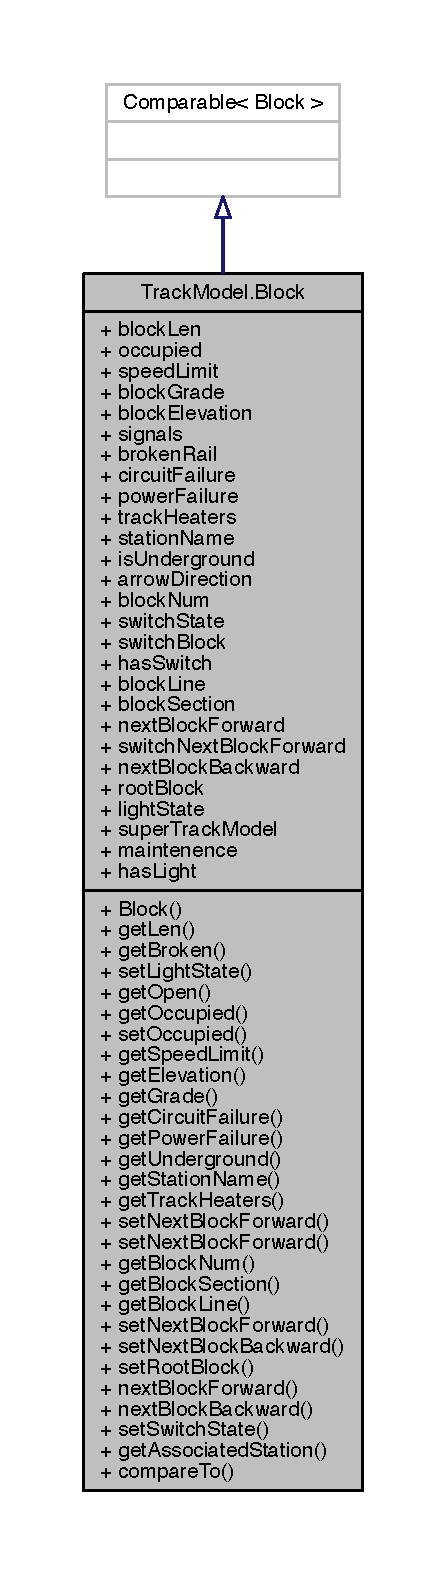
\includegraphics[height=550pt]{classTrackModel_1_1Block__inherit__graph}
\end{center}
\end{figure}


Collaboration diagram for Track\+Model.\+Block\+:
\nopagebreak
\begin{figure}[H]
\begin{center}
\leavevmode
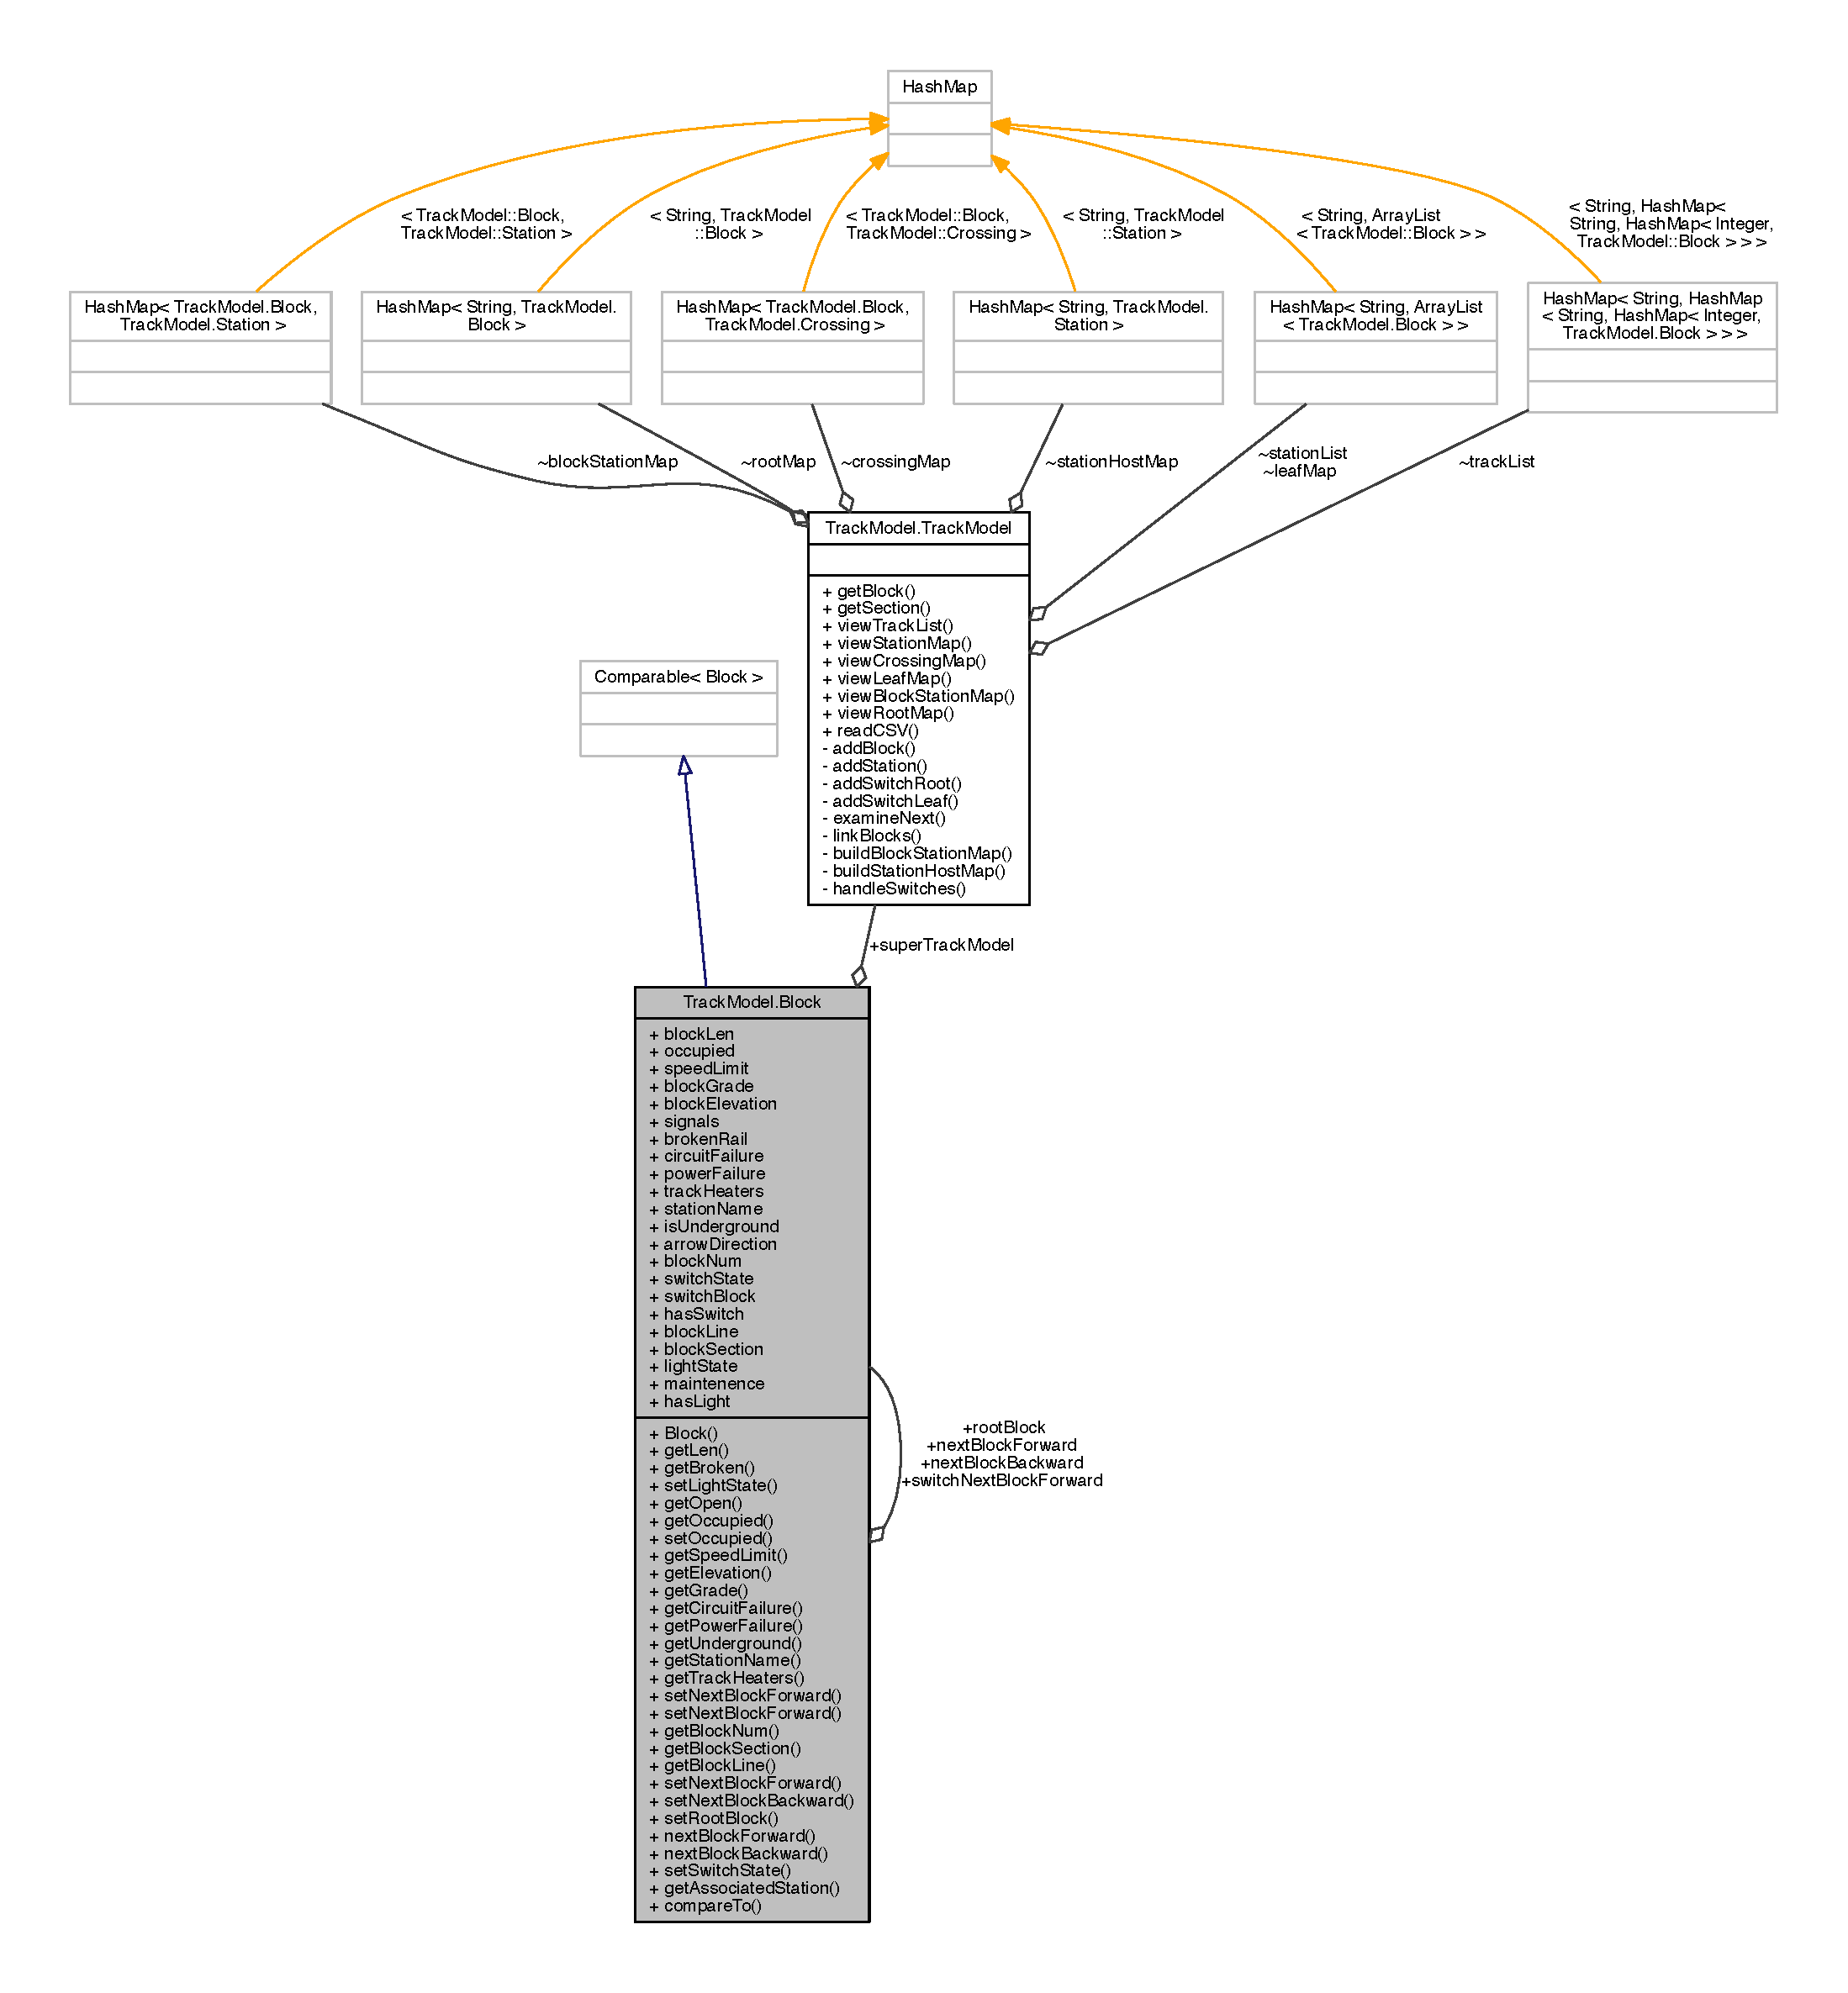
\includegraphics[width=350pt]{classTrackModel_1_1Block__coll__graph}
\end{center}
\end{figure}
\subsection*{Public Member Functions}
\begin{DoxyCompactItemize}
\item 
\hyperlink{classTrackModel_1_1Block_a016adcf378ac0c1738bd95a4db52f913}{Block} (\hyperlink{classTrackModel_1_1TrackModel}{Track\+Model} track, Boolean \hyperlink{classTrackModel_1_1Block_a000b5a3720b78b92062bbd2a9c560f6a}{occupied}, Boolean \hyperlink{classTrackModel_1_1Block_a3cb044acc87b68c2f7e482c2cdfdeab2}{is\+Underground}, Double \hyperlink{classTrackModel_1_1Block_a2272dc912ea46c59930f09258668a833}{block\+Len}, Double \hyperlink{classTrackModel_1_1Block_a445ba69829a748448595df9e048cc2ab}{block\+Grade}, Double elevation, Double \hyperlink{classTrackModel_1_1Block_a62ab3ddedf85055005dfdd4402716e65}{speed\+Limit}, String \hyperlink{classTrackModel_1_1Block_a178efb49178fd7418c6391ea3e35f106}{station\+Name}, String \hyperlink{classTrackModel_1_1Block_ad5c1ad3ac7452483c42dec413dbb63ab}{arrow\+Direction}, String \hyperlink{classTrackModel_1_1Block_a04e22a2597bed95ae3ed8f723b63de94}{block\+Line}, String \hyperlink{classTrackModel_1_1Block_a2adc620752945c54ae212bc4b6043975}{block\+Section}, Integer \hyperlink{classTrackModel_1_1Block_a429f329eb3c1e2ff40389df240f02b00}{block\+Num}, Boolean \hyperlink{classTrackModel_1_1Block_a1970e1588e5e0645096dc13094b640ff}{has\+Switch}, String \hyperlink{classTrackModel_1_1Block_a04565d6aa499ef51700e9e69d290e7e0}{switch\+Block})
\item 
Double \hyperlink{classTrackModel_1_1Block_af62e4fd52ba4f65098dd76ef8382fdde}{get\+Len} ()
\begin{DoxyCompactList}\small\item\em Returns the length of a block object. \end{DoxyCompactList}\item 
Boolean \hyperlink{classTrackModel_1_1Block_aa1ac9505793be31e681ef21dba05b85a}{get\+Broken} ()
\item 
Boolean \hyperlink{classTrackModel_1_1Block_ade3dc0b39ce6d111e7491443b052051e}{set\+Light\+State} (Integer set\+Int)
\begin{DoxyCompactList}\small\item\em Setter for the Wayside Controller module to set a light state based upon an Integer Maps 1 to true, 0 to false based upon the track internal convention. \end{DoxyCompactList}\item 
Boolean \hyperlink{classTrackModel_1_1Block_a5488f8e2329f780616c0189d31269a85}{get\+Open} ()
\begin{DoxyCompactList}\small\item\em Returns if a track block is open or not based upon the state of the breakages of a block. \end{DoxyCompactList}\item 
Boolean \hyperlink{classTrackModel_1_1Block_abd32beccef518c0e4622b2df1fd4ed54}{get\+Occupied} ()
\begin{DoxyCompactList}\small\item\em Returns the occupied state of a given block object. \end{DoxyCompactList}\item 
void \hyperlink{classTrackModel_1_1Block_a5a3c1477275fe3e3c7d0aaf4d7c32449}{set\+Occupied} ()
\item 
Double \hyperlink{classTrackModel_1_1Block_a68017a799915e4ef46455537ef41d124}{get\+Speed\+Limit} ()
\begin{DoxyCompactList}\small\item\em Returns the speed limit of a given block. \end{DoxyCompactList}\item 
Double \hyperlink{classTrackModel_1_1Block_a81c9de1ea89cce3046e9b6efc17871da}{get\+Elevation} ()
\begin{DoxyCompactList}\small\item\em Returns the cumulative elevation of a given blcok. \end{DoxyCompactList}\item 
Double \hyperlink{classTrackModel_1_1Block_ac33d34db48b02b47a035172af6025a7e}{get\+Grade} ()
\begin{DoxyCompactList}\small\item\em Returns the grade of a given block. \end{DoxyCompactList}\item 
Boolean \hyperlink{classTrackModel_1_1Block_a357ab105c5108e9656d10954fab85426}{get\+Circuit\+Failure} ()
\item 
Boolean \hyperlink{classTrackModel_1_1Block_abcfeb805be53d52f8034ba3eb629299d}{get\+Power\+Failure} ()
\item 
Boolean \hyperlink{classTrackModel_1_1Block_a8e946c966bec108e6540a6dc2321515e}{get\+Underground} ()
\item 
String \hyperlink{classTrackModel_1_1Block_a4fa53c36ff1ba06c6178dc651fd9bc4e}{get\+Station\+Name} ()
\item 
Boolean \hyperlink{classTrackModel_1_1Block_a43a18b38c61438d59621511020559b11}{get\+Track\+Heaters} ()
\item 
void \hyperlink{classTrackModel_1_1Block_a5b78735684cbae8d24cea8874f27e5bd}{set\+Next\+Block\+Forward} ()
\item 
void \hyperlink{classTrackModel_1_1Block_a01715a2edb54f2a6791f95e81e613f2b}{set\+Next\+Block\+Forward} (\hyperlink{classTrackModel_1_1Block}{Block} set\+Block)
\item 
Integer \hyperlink{classTrackModel_1_1Block_a715fbe2efb7d55f92eab33cb635a4a00}{get\+Block\+Num} ()
\item 
String \hyperlink{classTrackModel_1_1Block_a2733e908ed59561bcb58ada3dd6045ab}{get\+Block\+Section} ()
\begin{DoxyCompactList}\small\item\em Returns the section a block is on. \end{DoxyCompactList}\item 
String \hyperlink{classTrackModel_1_1Block_a6f5a001898b82c18e371aebeca433eec}{get\+Block\+Line} ()
\begin{DoxyCompactList}\small\item\em Returns the line a block is on. \end{DoxyCompactList}\item 
void \hyperlink{classTrackModel_1_1Block_a737780636e43298572855b15fc3b20d5}{set\+Next\+Block\+Forward} (\hyperlink{classTrackModel_1_1Block}{Block} low\+Block, \hyperlink{classTrackModel_1_1Block}{Block} high\+Block)
\begin{DoxyCompactList}\small\item\em Setter for the next block forward in the condition for a switch is present. \end{DoxyCompactList}\item 
void \hyperlink{classTrackModel_1_1Block_ad0364d9a5fb2741523cca7abd356d3e9}{set\+Next\+Block\+Backward} (\hyperlink{classTrackModel_1_1Block}{Block} set\+Block)
\begin{DoxyCompactList}\small\item\em Sets the next block in the \char`\"{}reverse\char`\"{} direction. \end{DoxyCompactList}\item 
void \hyperlink{classTrackModel_1_1Block_a07ebf377b8be2509705a1fbb5e48e98b}{set\+Root\+Block} (\hyperlink{classTrackModel_1_1Block}{Block} \hyperlink{classTrackModel_1_1Block_a400d119c96231f6cf5db4accbf48cb84}{root\+Block})
\begin{DoxyCompactList}\small\item\em Sets the root block in the \char`\"{}reverse\char`\"{} direction to deal with switch conditions. \end{DoxyCompactList}\item 
\hyperlink{classTrackModel_1_1Block}{Block} \hyperlink{classTrackModel_1_1Block_a5b41d49bee482917bbc5d3af78c25020}{next\+Block\+Forward} ()
\begin{DoxyCompactList}\small\item\em Gets the next block forward along based upon the current switch state. \end{DoxyCompactList}\item 
\hyperlink{classTrackModel_1_1Block}{Block} \hyperlink{classTrackModel_1_1Block_a0ea37da4be949e0734cd7c6db555013e}{next\+Block\+Backward} ()
\item 
Boolean \hyperlink{classTrackModel_1_1Block_aa206833e61700249e5905fe6e6126399}{set\+Switch\+State} (Integer set\+Int)
\begin{DoxyCompactList}\small\item\em Setter for the Wayside Controller module to set a switch state based upon an Integer Maps 1 to true, 0 to false based upon the track internal convention. \end{DoxyCompactList}\item 
\hyperlink{classTrackModel_1_1Station}{Station} \hyperlink{classTrackModel_1_1Block_ad01125a6c501452bf33320b01471a24a}{get\+Associated\+Station} ()
\begin{DoxyCompactList}\small\item\em Returns the associated station of the block. \end{DoxyCompactList}\item 
int \hyperlink{classTrackModel_1_1Block_a2b940992804680c1146a1fef8f55f7db}{compare\+To} (\hyperlink{classTrackModel_1_1Block}{Block} that\+Block)
\begin{DoxyCompactList}\small\item\em Implements the comparable interface for blocks via the associalted block\+Num of a given block. \end{DoxyCompactList}\end{DoxyCompactItemize}
\subsection*{Public Attributes}
\begin{DoxyCompactItemize}
\item 
Double \hyperlink{classTrackModel_1_1Block_a2272dc912ea46c59930f09258668a833}{block\+Len}
\item 
Boolean \hyperlink{classTrackModel_1_1Block_a000b5a3720b78b92062bbd2a9c560f6a}{occupied}
\item 
Double \hyperlink{classTrackModel_1_1Block_a62ab3ddedf85055005dfdd4402716e65}{speed\+Limit}
\item 
Double \hyperlink{classTrackModel_1_1Block_a445ba69829a748448595df9e048cc2ab}{block\+Grade}
\item 
Double \hyperlink{classTrackModel_1_1Block_ab26ac3adf1ce690a6e187df65f730b0d}{block\+Elevation}
\item 
Boolean \hyperlink{classTrackModel_1_1Block_a7fd1ac5eadeb3dd29da9fab51c8c26f2}{signals}
\item 
Boolean \hyperlink{classTrackModel_1_1Block_a059c0f4f0b6f5d7b50deee6f13538bab}{broken\+Rail}
\item 
Boolean \hyperlink{classTrackModel_1_1Block_a90373dff7852d248a540bd9d9f0514cb}{circuit\+Failure}
\item 
Boolean \hyperlink{classTrackModel_1_1Block_a1c69717cb3818955e60763bc8f4dff8a}{power\+Failure}
\item 
Boolean \hyperlink{classTrackModel_1_1Block_afd3cf37d0f925e0440179716b2ad2730}{track\+Heaters}
\item 
String \hyperlink{classTrackModel_1_1Block_a178efb49178fd7418c6391ea3e35f106}{station\+Name}
\item 
Boolean \hyperlink{classTrackModel_1_1Block_a3cb044acc87b68c2f7e482c2cdfdeab2}{is\+Underground}
\item 
String \hyperlink{classTrackModel_1_1Block_ad5c1ad3ac7452483c42dec413dbb63ab}{arrow\+Direction}
\item 
Integer \hyperlink{classTrackModel_1_1Block_a429f329eb3c1e2ff40389df240f02b00}{block\+Num}
\item 
Boolean \hyperlink{classTrackModel_1_1Block_a5c2a0d414f6cca8552f476dd12e94d3f}{switch\+State}
\item 
String \hyperlink{classTrackModel_1_1Block_a04565d6aa499ef51700e9e69d290e7e0}{switch\+Block}
\item 
Boolean \hyperlink{classTrackModel_1_1Block_a1970e1588e5e0645096dc13094b640ff}{has\+Switch}
\item 
String \hyperlink{classTrackModel_1_1Block_a04e22a2597bed95ae3ed8f723b63de94}{block\+Line}
\item 
String \hyperlink{classTrackModel_1_1Block_a2adc620752945c54ae212bc4b6043975}{block\+Section}
\item 
\hyperlink{classTrackModel_1_1Block}{Block} \hyperlink{classTrackModel_1_1Block_acd730e762fcf625825d4939bc38b2672}{next\+Block\+Forward}
\item 
\hyperlink{classTrackModel_1_1Block}{Block} \hyperlink{classTrackModel_1_1Block_a8a7d15ff05ed0c3a56e34c27c06dd99a}{switch\+Next\+Block\+Forward}
\item 
\hyperlink{classTrackModel_1_1Block}{Block} \hyperlink{classTrackModel_1_1Block_a267092cfc33a1a5b06d61e605aa16da5}{next\+Block\+Backward}
\item 
\hyperlink{classTrackModel_1_1Block}{Block} \hyperlink{classTrackModel_1_1Block_a400d119c96231f6cf5db4accbf48cb84}{root\+Block}
\item 
Boolean \hyperlink{classTrackModel_1_1Block_ae2a73faa62ffb87e3a70e72c6bdec27d}{light\+State}
\item 
\hyperlink{classTrackModel_1_1TrackModel}{Track\+Model} \hyperlink{classTrackModel_1_1Block_a62ba712491f00e90cc279365a693f00f}{super\+Track\+Model}
\item 
Boolean \hyperlink{classTrackModel_1_1Block_a2a4f17aa957073179dd40a0fb5343fbc}{maintenence}
\item 
Boolean \hyperlink{classTrackModel_1_1Block_a1cfc614674d2e3ddc91aae595d8c2f83}{has\+Light}
\end{DoxyCompactItemize}


\subsection{Constructor \& Destructor Documentation}
\mbox{\Hypertarget{classTrackModel_1_1Block_a016adcf378ac0c1738bd95a4db52f913}\label{classTrackModel_1_1Block_a016adcf378ac0c1738bd95a4db52f913}} 
\index{Track\+Model\+::\+Block@{Track\+Model\+::\+Block}!Block@{Block}}
\index{Block@{Block}!Track\+Model\+::\+Block@{Track\+Model\+::\+Block}}
\subsubsection{\texorpdfstring{Block()}{Block()}}
{\footnotesize\ttfamily Track\+Model.\+Block.\+Block (\begin{DoxyParamCaption}\item[{\hyperlink{classTrackModel_1_1TrackModel}{Track\+Model}}]{track,  }\item[{Boolean}]{occupied,  }\item[{Boolean}]{is\+Underground,  }\item[{Double}]{block\+Len,  }\item[{Double}]{block\+Grade,  }\item[{Double}]{elevation,  }\item[{Double}]{speed\+Limit,  }\item[{String}]{station\+Name,  }\item[{String}]{arrow\+Direction,  }\item[{String}]{block\+Line,  }\item[{String}]{block\+Section,  }\item[{Integer}]{block\+Num,  }\item[{Boolean}]{has\+Switch,  }\item[{String}]{switch\+Block }\end{DoxyParamCaption})}



\subsection{Member Function Documentation}
\mbox{\Hypertarget{classTrackModel_1_1Block_a2b940992804680c1146a1fef8f55f7db}\label{classTrackModel_1_1Block_a2b940992804680c1146a1fef8f55f7db}} 
\index{Track\+Model\+::\+Block@{Track\+Model\+::\+Block}!compare\+To@{compare\+To}}
\index{compare\+To@{compare\+To}!Track\+Model\+::\+Block@{Track\+Model\+::\+Block}}
\subsubsection{\texorpdfstring{compare\+To()}{compareTo()}}
{\footnotesize\ttfamily int Track\+Model.\+Block.\+compare\+To (\begin{DoxyParamCaption}\item[{\hyperlink{classTrackModel_1_1Block}{Block}}]{that\+Block }\end{DoxyParamCaption})}



Implements the comparable interface for blocks via the associalted block\+Num of a given block. 

At this time, this implementation does not verify that blocks are the same across lines. \mbox{\Hypertarget{classTrackModel_1_1Block_ad01125a6c501452bf33320b01471a24a}\label{classTrackModel_1_1Block_ad01125a6c501452bf33320b01471a24a}} 
\index{Track\+Model\+::\+Block@{Track\+Model\+::\+Block}!get\+Associated\+Station@{get\+Associated\+Station}}
\index{get\+Associated\+Station@{get\+Associated\+Station}!Track\+Model\+::\+Block@{Track\+Model\+::\+Block}}
\subsubsection{\texorpdfstring{get\+Associated\+Station()}{getAssociatedStation()}}
{\footnotesize\ttfamily \hyperlink{classTrackModel_1_1Station}{Station} Track\+Model.\+Block.\+get\+Associated\+Station (\begin{DoxyParamCaption}{ }\end{DoxyParamCaption})}



Returns the associated station of the block. 

\begin{DoxyReturn}{Returns}
the \hyperlink{classTrackModel_1_1Station}{Station} object of the associated block 
\end{DoxyReturn}
\mbox{\Hypertarget{classTrackModel_1_1Block_a6f5a001898b82c18e371aebeca433eec}\label{classTrackModel_1_1Block_a6f5a001898b82c18e371aebeca433eec}} 
\index{Track\+Model\+::\+Block@{Track\+Model\+::\+Block}!get\+Block\+Line@{get\+Block\+Line}}
\index{get\+Block\+Line@{get\+Block\+Line}!Track\+Model\+::\+Block@{Track\+Model\+::\+Block}}
\subsubsection{\texorpdfstring{get\+Block\+Line()}{getBlockLine()}}
{\footnotesize\ttfamily String Track\+Model.\+Block.\+get\+Block\+Line (\begin{DoxyParamCaption}{ }\end{DoxyParamCaption})}



Returns the line a block is on. 

\mbox{\Hypertarget{classTrackModel_1_1Block_a715fbe2efb7d55f92eab33cb635a4a00}\label{classTrackModel_1_1Block_a715fbe2efb7d55f92eab33cb635a4a00}} 
\index{Track\+Model\+::\+Block@{Track\+Model\+::\+Block}!get\+Block\+Num@{get\+Block\+Num}}
\index{get\+Block\+Num@{get\+Block\+Num}!Track\+Model\+::\+Block@{Track\+Model\+::\+Block}}
\subsubsection{\texorpdfstring{get\+Block\+Num()}{getBlockNum()}}
{\footnotesize\ttfamily Integer Track\+Model.\+Block.\+get\+Block\+Num (\begin{DoxyParamCaption}{ }\end{DoxyParamCaption})}

\mbox{\Hypertarget{classTrackModel_1_1Block_a2733e908ed59561bcb58ada3dd6045ab}\label{classTrackModel_1_1Block_a2733e908ed59561bcb58ada3dd6045ab}} 
\index{Track\+Model\+::\+Block@{Track\+Model\+::\+Block}!get\+Block\+Section@{get\+Block\+Section}}
\index{get\+Block\+Section@{get\+Block\+Section}!Track\+Model\+::\+Block@{Track\+Model\+::\+Block}}
\subsubsection{\texorpdfstring{get\+Block\+Section()}{getBlockSection()}}
{\footnotesize\ttfamily String Track\+Model.\+Block.\+get\+Block\+Section (\begin{DoxyParamCaption}{ }\end{DoxyParamCaption})}



Returns the section a block is on. 

\mbox{\Hypertarget{classTrackModel_1_1Block_aa1ac9505793be31e681ef21dba05b85a}\label{classTrackModel_1_1Block_aa1ac9505793be31e681ef21dba05b85a}} 
\index{Track\+Model\+::\+Block@{Track\+Model\+::\+Block}!get\+Broken@{get\+Broken}}
\index{get\+Broken@{get\+Broken}!Track\+Model\+::\+Block@{Track\+Model\+::\+Block}}
\subsubsection{\texorpdfstring{get\+Broken()}{getBroken()}}
{\footnotesize\ttfamily Boolean Track\+Model.\+Block.\+get\+Broken (\begin{DoxyParamCaption}{ }\end{DoxyParamCaption})}

\mbox{\Hypertarget{classTrackModel_1_1Block_a357ab105c5108e9656d10954fab85426}\label{classTrackModel_1_1Block_a357ab105c5108e9656d10954fab85426}} 
\index{Track\+Model\+::\+Block@{Track\+Model\+::\+Block}!get\+Circuit\+Failure@{get\+Circuit\+Failure}}
\index{get\+Circuit\+Failure@{get\+Circuit\+Failure}!Track\+Model\+::\+Block@{Track\+Model\+::\+Block}}
\subsubsection{\texorpdfstring{get\+Circuit\+Failure()}{getCircuitFailure()}}
{\footnotesize\ttfamily Boolean Track\+Model.\+Block.\+get\+Circuit\+Failure (\begin{DoxyParamCaption}{ }\end{DoxyParamCaption})}

\mbox{\Hypertarget{classTrackModel_1_1Block_a81c9de1ea89cce3046e9b6efc17871da}\label{classTrackModel_1_1Block_a81c9de1ea89cce3046e9b6efc17871da}} 
\index{Track\+Model\+::\+Block@{Track\+Model\+::\+Block}!get\+Elevation@{get\+Elevation}}
\index{get\+Elevation@{get\+Elevation}!Track\+Model\+::\+Block@{Track\+Model\+::\+Block}}
\subsubsection{\texorpdfstring{get\+Elevation()}{getElevation()}}
{\footnotesize\ttfamily Double Track\+Model.\+Block.\+get\+Elevation (\begin{DoxyParamCaption}{ }\end{DoxyParamCaption})}



Returns the cumulative elevation of a given blcok. 

\mbox{\Hypertarget{classTrackModel_1_1Block_ac33d34db48b02b47a035172af6025a7e}\label{classTrackModel_1_1Block_ac33d34db48b02b47a035172af6025a7e}} 
\index{Track\+Model\+::\+Block@{Track\+Model\+::\+Block}!get\+Grade@{get\+Grade}}
\index{get\+Grade@{get\+Grade}!Track\+Model\+::\+Block@{Track\+Model\+::\+Block}}
\subsubsection{\texorpdfstring{get\+Grade()}{getGrade()}}
{\footnotesize\ttfamily Double Track\+Model.\+Block.\+get\+Grade (\begin{DoxyParamCaption}{ }\end{DoxyParamCaption})}



Returns the grade of a given block. 

\mbox{\Hypertarget{classTrackModel_1_1Block_af62e4fd52ba4f65098dd76ef8382fdde}\label{classTrackModel_1_1Block_af62e4fd52ba4f65098dd76ef8382fdde}} 
\index{Track\+Model\+::\+Block@{Track\+Model\+::\+Block}!get\+Len@{get\+Len}}
\index{get\+Len@{get\+Len}!Track\+Model\+::\+Block@{Track\+Model\+::\+Block}}
\subsubsection{\texorpdfstring{get\+Len()}{getLen()}}
{\footnotesize\ttfamily Double Track\+Model.\+Block.\+get\+Len (\begin{DoxyParamCaption}{ }\end{DoxyParamCaption})}



Returns the length of a block object. 

\mbox{\Hypertarget{classTrackModel_1_1Block_abd32beccef518c0e4622b2df1fd4ed54}\label{classTrackModel_1_1Block_abd32beccef518c0e4622b2df1fd4ed54}} 
\index{Track\+Model\+::\+Block@{Track\+Model\+::\+Block}!get\+Occupied@{get\+Occupied}}
\index{get\+Occupied@{get\+Occupied}!Track\+Model\+::\+Block@{Track\+Model\+::\+Block}}
\subsubsection{\texorpdfstring{get\+Occupied()}{getOccupied()}}
{\footnotesize\ttfamily Boolean Track\+Model.\+Block.\+get\+Occupied (\begin{DoxyParamCaption}{ }\end{DoxyParamCaption})}



Returns the occupied state of a given block object. 

\mbox{\Hypertarget{classTrackModel_1_1Block_a5488f8e2329f780616c0189d31269a85}\label{classTrackModel_1_1Block_a5488f8e2329f780616c0189d31269a85}} 
\index{Track\+Model\+::\+Block@{Track\+Model\+::\+Block}!get\+Open@{get\+Open}}
\index{get\+Open@{get\+Open}!Track\+Model\+::\+Block@{Track\+Model\+::\+Block}}
\subsubsection{\texorpdfstring{get\+Open()}{getOpen()}}
{\footnotesize\ttfamily Boolean Track\+Model.\+Block.\+get\+Open (\begin{DoxyParamCaption}{ }\end{DoxyParamCaption})}



Returns if a track block is open or not based upon the state of the breakages of a block. 

\mbox{\Hypertarget{classTrackModel_1_1Block_abcfeb805be53d52f8034ba3eb629299d}\label{classTrackModel_1_1Block_abcfeb805be53d52f8034ba3eb629299d}} 
\index{Track\+Model\+::\+Block@{Track\+Model\+::\+Block}!get\+Power\+Failure@{get\+Power\+Failure}}
\index{get\+Power\+Failure@{get\+Power\+Failure}!Track\+Model\+::\+Block@{Track\+Model\+::\+Block}}
\subsubsection{\texorpdfstring{get\+Power\+Failure()}{getPowerFailure()}}
{\footnotesize\ttfamily Boolean Track\+Model.\+Block.\+get\+Power\+Failure (\begin{DoxyParamCaption}{ }\end{DoxyParamCaption})}

\mbox{\Hypertarget{classTrackModel_1_1Block_a68017a799915e4ef46455537ef41d124}\label{classTrackModel_1_1Block_a68017a799915e4ef46455537ef41d124}} 
\index{Track\+Model\+::\+Block@{Track\+Model\+::\+Block}!get\+Speed\+Limit@{get\+Speed\+Limit}}
\index{get\+Speed\+Limit@{get\+Speed\+Limit}!Track\+Model\+::\+Block@{Track\+Model\+::\+Block}}
\subsubsection{\texorpdfstring{get\+Speed\+Limit()}{getSpeedLimit()}}
{\footnotesize\ttfamily Double Track\+Model.\+Block.\+get\+Speed\+Limit (\begin{DoxyParamCaption}{ }\end{DoxyParamCaption})}



Returns the speed limit of a given block. 

\mbox{\Hypertarget{classTrackModel_1_1Block_a4fa53c36ff1ba06c6178dc651fd9bc4e}\label{classTrackModel_1_1Block_a4fa53c36ff1ba06c6178dc651fd9bc4e}} 
\index{Track\+Model\+::\+Block@{Track\+Model\+::\+Block}!get\+Station\+Name@{get\+Station\+Name}}
\index{get\+Station\+Name@{get\+Station\+Name}!Track\+Model\+::\+Block@{Track\+Model\+::\+Block}}
\subsubsection{\texorpdfstring{get\+Station\+Name()}{getStationName()}}
{\footnotesize\ttfamily String Track\+Model.\+Block.\+get\+Station\+Name (\begin{DoxyParamCaption}{ }\end{DoxyParamCaption})}

\mbox{\Hypertarget{classTrackModel_1_1Block_a43a18b38c61438d59621511020559b11}\label{classTrackModel_1_1Block_a43a18b38c61438d59621511020559b11}} 
\index{Track\+Model\+::\+Block@{Track\+Model\+::\+Block}!get\+Track\+Heaters@{get\+Track\+Heaters}}
\index{get\+Track\+Heaters@{get\+Track\+Heaters}!Track\+Model\+::\+Block@{Track\+Model\+::\+Block}}
\subsubsection{\texorpdfstring{get\+Track\+Heaters()}{getTrackHeaters()}}
{\footnotesize\ttfamily Boolean Track\+Model.\+Block.\+get\+Track\+Heaters (\begin{DoxyParamCaption}{ }\end{DoxyParamCaption})}

\mbox{\Hypertarget{classTrackModel_1_1Block_a8e946c966bec108e6540a6dc2321515e}\label{classTrackModel_1_1Block_a8e946c966bec108e6540a6dc2321515e}} 
\index{Track\+Model\+::\+Block@{Track\+Model\+::\+Block}!get\+Underground@{get\+Underground}}
\index{get\+Underground@{get\+Underground}!Track\+Model\+::\+Block@{Track\+Model\+::\+Block}}
\subsubsection{\texorpdfstring{get\+Underground()}{getUnderground()}}
{\footnotesize\ttfamily Boolean Track\+Model.\+Block.\+get\+Underground (\begin{DoxyParamCaption}{ }\end{DoxyParamCaption})}

\mbox{\Hypertarget{classTrackModel_1_1Block_a0ea37da4be949e0734cd7c6db555013e}\label{classTrackModel_1_1Block_a0ea37da4be949e0734cd7c6db555013e}} 
\index{Track\+Model\+::\+Block@{Track\+Model\+::\+Block}!next\+Block\+Backward@{next\+Block\+Backward}}
\index{next\+Block\+Backward@{next\+Block\+Backward}!Track\+Model\+::\+Block@{Track\+Model\+::\+Block}}
\subsubsection{\texorpdfstring{next\+Block\+Backward()}{nextBlockBackward()}}
{\footnotesize\ttfamily \hyperlink{classTrackModel_1_1Block}{Block} Track\+Model.\+Block.\+next\+Block\+Backward (\begin{DoxyParamCaption}{ }\end{DoxyParamCaption})}

\mbox{\Hypertarget{classTrackModel_1_1Block_a5b41d49bee482917bbc5d3af78c25020}\label{classTrackModel_1_1Block_a5b41d49bee482917bbc5d3af78c25020}} 
\index{Track\+Model\+::\+Block@{Track\+Model\+::\+Block}!next\+Block\+Forward@{next\+Block\+Forward}}
\index{next\+Block\+Forward@{next\+Block\+Forward}!Track\+Model\+::\+Block@{Track\+Model\+::\+Block}}
\subsubsection{\texorpdfstring{next\+Block\+Forward()}{nextBlockForward()}}
{\footnotesize\ttfamily \hyperlink{classTrackModel_1_1Block}{Block} Track\+Model.\+Block.\+next\+Block\+Forward (\begin{DoxyParamCaption}{ }\end{DoxyParamCaption})}



Gets the next block forward along based upon the current switch state. 

If there is no switch, it returns the next block \mbox{\Hypertarget{classTrackModel_1_1Block_ade3dc0b39ce6d111e7491443b052051e}\label{classTrackModel_1_1Block_ade3dc0b39ce6d111e7491443b052051e}} 
\index{Track\+Model\+::\+Block@{Track\+Model\+::\+Block}!set\+Light\+State@{set\+Light\+State}}
\index{set\+Light\+State@{set\+Light\+State}!Track\+Model\+::\+Block@{Track\+Model\+::\+Block}}
\subsubsection{\texorpdfstring{set\+Light\+State()}{setLightState()}}
{\footnotesize\ttfamily Boolean Track\+Model.\+Block.\+set\+Light\+State (\begin{DoxyParamCaption}\item[{Integer}]{set\+Int }\end{DoxyParamCaption})}



Setter for the Wayside Controller module to set a light state based upon an Integer Maps 1 to true, 0 to false based upon the track internal convention. 


\begin{DoxyParams}{Parameters}
{\em set\+Int} & integer for the switch state to be set to \\
\hline
\end{DoxyParams}
\begin{DoxyRefDesc}{Todo}
\item[\hyperlink{todo__todo000001}{Todo}]Add strict value assertions that set\+Int is either 0 or 1 \end{DoxyRefDesc}
\mbox{\Hypertarget{classTrackModel_1_1Block_ad0364d9a5fb2741523cca7abd356d3e9}\label{classTrackModel_1_1Block_ad0364d9a5fb2741523cca7abd356d3e9}} 
\index{Track\+Model\+::\+Block@{Track\+Model\+::\+Block}!set\+Next\+Block\+Backward@{set\+Next\+Block\+Backward}}
\index{set\+Next\+Block\+Backward@{set\+Next\+Block\+Backward}!Track\+Model\+::\+Block@{Track\+Model\+::\+Block}}
\subsubsection{\texorpdfstring{set\+Next\+Block\+Backward()}{setNextBlockBackward()}}
{\footnotesize\ttfamily void Track\+Model.\+Block.\+set\+Next\+Block\+Backward (\begin{DoxyParamCaption}\item[{\hyperlink{classTrackModel_1_1Block}{Block}}]{set\+Block }\end{DoxyParamCaption})}



Sets the next block in the \char`\"{}reverse\char`\"{} direction. 

Does not handle switch conditions 
\begin{DoxyParams}{Parameters}
{\em set\+Block} & the block to set the default backwards block to \\
\hline
\end{DoxyParams}
\mbox{\Hypertarget{classTrackModel_1_1Block_a5b78735684cbae8d24cea8874f27e5bd}\label{classTrackModel_1_1Block_a5b78735684cbae8d24cea8874f27e5bd}} 
\index{Track\+Model\+::\+Block@{Track\+Model\+::\+Block}!set\+Next\+Block\+Forward@{set\+Next\+Block\+Forward}}
\index{set\+Next\+Block\+Forward@{set\+Next\+Block\+Forward}!Track\+Model\+::\+Block@{Track\+Model\+::\+Block}}
\subsubsection{\texorpdfstring{set\+Next\+Block\+Forward()}{setNextBlockForward()}\hspace{0.1cm}{\footnotesize\ttfamily [1/3]}}
{\footnotesize\ttfamily void Track\+Model.\+Block.\+set\+Next\+Block\+Forward (\begin{DoxyParamCaption}{ }\end{DoxyParamCaption})}

\mbox{\Hypertarget{classTrackModel_1_1Block_a01715a2edb54f2a6791f95e81e613f2b}\label{classTrackModel_1_1Block_a01715a2edb54f2a6791f95e81e613f2b}} 
\index{Track\+Model\+::\+Block@{Track\+Model\+::\+Block}!set\+Next\+Block\+Forward@{set\+Next\+Block\+Forward}}
\index{set\+Next\+Block\+Forward@{set\+Next\+Block\+Forward}!Track\+Model\+::\+Block@{Track\+Model\+::\+Block}}
\subsubsection{\texorpdfstring{set\+Next\+Block\+Forward()}{setNextBlockForward()}\hspace{0.1cm}{\footnotesize\ttfamily [2/3]}}
{\footnotesize\ttfamily void Track\+Model.\+Block.\+set\+Next\+Block\+Forward (\begin{DoxyParamCaption}\item[{\hyperlink{classTrackModel_1_1Block}{Block}}]{set\+Block }\end{DoxyParamCaption})}

\mbox{\Hypertarget{classTrackModel_1_1Block_a737780636e43298572855b15fc3b20d5}\label{classTrackModel_1_1Block_a737780636e43298572855b15fc3b20d5}} 
\index{Track\+Model\+::\+Block@{Track\+Model\+::\+Block}!set\+Next\+Block\+Forward@{set\+Next\+Block\+Forward}}
\index{set\+Next\+Block\+Forward@{set\+Next\+Block\+Forward}!Track\+Model\+::\+Block@{Track\+Model\+::\+Block}}
\subsubsection{\texorpdfstring{set\+Next\+Block\+Forward()}{setNextBlockForward()}\hspace{0.1cm}{\footnotesize\ttfamily [3/3]}}
{\footnotesize\ttfamily void Track\+Model.\+Block.\+set\+Next\+Block\+Forward (\begin{DoxyParamCaption}\item[{\hyperlink{classTrackModel_1_1Block}{Block}}]{low\+Block,  }\item[{\hyperlink{classTrackModel_1_1Block}{Block}}]{high\+Block }\end{DoxyParamCaption})}



Setter for the next block forward in the condition for a switch is present. 

By default, initializes the switch to the lower block (as determined by block\+Num) to be destination when the this.\+switch\+State = true \mbox{\Hypertarget{classTrackModel_1_1Block_a5a3c1477275fe3e3c7d0aaf4d7c32449}\label{classTrackModel_1_1Block_a5a3c1477275fe3e3c7d0aaf4d7c32449}} 
\index{Track\+Model\+::\+Block@{Track\+Model\+::\+Block}!set\+Occupied@{set\+Occupied}}
\index{set\+Occupied@{set\+Occupied}!Track\+Model\+::\+Block@{Track\+Model\+::\+Block}}
\subsubsection{\texorpdfstring{set\+Occupied()}{setOccupied()}}
{\footnotesize\ttfamily void Track\+Model.\+Block.\+set\+Occupied (\begin{DoxyParamCaption}{ }\end{DoxyParamCaption})}

\mbox{\Hypertarget{classTrackModel_1_1Block_a07ebf377b8be2509705a1fbb5e48e98b}\label{classTrackModel_1_1Block_a07ebf377b8be2509705a1fbb5e48e98b}} 
\index{Track\+Model\+::\+Block@{Track\+Model\+::\+Block}!set\+Root\+Block@{set\+Root\+Block}}
\index{set\+Root\+Block@{set\+Root\+Block}!Track\+Model\+::\+Block@{Track\+Model\+::\+Block}}
\subsubsection{\texorpdfstring{set\+Root\+Block()}{setRootBlock()}}
{\footnotesize\ttfamily void Track\+Model.\+Block.\+set\+Root\+Block (\begin{DoxyParamCaption}\item[{\hyperlink{classTrackModel_1_1Block}{Block}}]{root\+Block }\end{DoxyParamCaption})}



Sets the root block in the \char`\"{}reverse\char`\"{} direction to deal with switch conditions. 


\begin{DoxyParams}{Parameters}
{\em root\+Block} & the root block backwards of a switch block \\
\hline
\end{DoxyParams}
\mbox{\Hypertarget{classTrackModel_1_1Block_aa206833e61700249e5905fe6e6126399}\label{classTrackModel_1_1Block_aa206833e61700249e5905fe6e6126399}} 
\index{Track\+Model\+::\+Block@{Track\+Model\+::\+Block}!set\+Switch\+State@{set\+Switch\+State}}
\index{set\+Switch\+State@{set\+Switch\+State}!Track\+Model\+::\+Block@{Track\+Model\+::\+Block}}
\subsubsection{\texorpdfstring{set\+Switch\+State()}{setSwitchState()}}
{\footnotesize\ttfamily Boolean Track\+Model.\+Block.\+set\+Switch\+State (\begin{DoxyParamCaption}\item[{Integer}]{set\+Int }\end{DoxyParamCaption})}



Setter for the Wayside Controller module to set a switch state based upon an Integer Maps 1 to true, 0 to false based upon the track internal convention. 


\begin{DoxyParams}{Parameters}
{\em set\+Int} & integer for the switch state to be set to \\
\hline
\end{DoxyParams}
\begin{DoxyRefDesc}{Todo}
\item[\hyperlink{todo__todo000002}{Todo}]Add strict value assertions that set\+Int is either 0 or 1 \end{DoxyRefDesc}


\subsection{Member Data Documentation}
\mbox{\Hypertarget{classTrackModel_1_1Block_ad5c1ad3ac7452483c42dec413dbb63ab}\label{classTrackModel_1_1Block_ad5c1ad3ac7452483c42dec413dbb63ab}} 
\index{Track\+Model\+::\+Block@{Track\+Model\+::\+Block}!arrow\+Direction@{arrow\+Direction}}
\index{arrow\+Direction@{arrow\+Direction}!Track\+Model\+::\+Block@{Track\+Model\+::\+Block}}
\subsubsection{\texorpdfstring{arrow\+Direction}{arrowDirection}}
{\footnotesize\ttfamily String Track\+Model.\+Block.\+arrow\+Direction}

\mbox{\Hypertarget{classTrackModel_1_1Block_ab26ac3adf1ce690a6e187df65f730b0d}\label{classTrackModel_1_1Block_ab26ac3adf1ce690a6e187df65f730b0d}} 
\index{Track\+Model\+::\+Block@{Track\+Model\+::\+Block}!block\+Elevation@{block\+Elevation}}
\index{block\+Elevation@{block\+Elevation}!Track\+Model\+::\+Block@{Track\+Model\+::\+Block}}
\subsubsection{\texorpdfstring{block\+Elevation}{blockElevation}}
{\footnotesize\ttfamily Double Track\+Model.\+Block.\+block\+Elevation}

\mbox{\Hypertarget{classTrackModel_1_1Block_a445ba69829a748448595df9e048cc2ab}\label{classTrackModel_1_1Block_a445ba69829a748448595df9e048cc2ab}} 
\index{Track\+Model\+::\+Block@{Track\+Model\+::\+Block}!block\+Grade@{block\+Grade}}
\index{block\+Grade@{block\+Grade}!Track\+Model\+::\+Block@{Track\+Model\+::\+Block}}
\subsubsection{\texorpdfstring{block\+Grade}{blockGrade}}
{\footnotesize\ttfamily Double Track\+Model.\+Block.\+block\+Grade}

\mbox{\Hypertarget{classTrackModel_1_1Block_a2272dc912ea46c59930f09258668a833}\label{classTrackModel_1_1Block_a2272dc912ea46c59930f09258668a833}} 
\index{Track\+Model\+::\+Block@{Track\+Model\+::\+Block}!block\+Len@{block\+Len}}
\index{block\+Len@{block\+Len}!Track\+Model\+::\+Block@{Track\+Model\+::\+Block}}
\subsubsection{\texorpdfstring{block\+Len}{blockLen}}
{\footnotesize\ttfamily Double Track\+Model.\+Block.\+block\+Len}

\mbox{\Hypertarget{classTrackModel_1_1Block_a04e22a2597bed95ae3ed8f723b63de94}\label{classTrackModel_1_1Block_a04e22a2597bed95ae3ed8f723b63de94}} 
\index{Track\+Model\+::\+Block@{Track\+Model\+::\+Block}!block\+Line@{block\+Line}}
\index{block\+Line@{block\+Line}!Track\+Model\+::\+Block@{Track\+Model\+::\+Block}}
\subsubsection{\texorpdfstring{block\+Line}{blockLine}}
{\footnotesize\ttfamily String Track\+Model.\+Block.\+block\+Line}

\mbox{\Hypertarget{classTrackModel_1_1Block_a429f329eb3c1e2ff40389df240f02b00}\label{classTrackModel_1_1Block_a429f329eb3c1e2ff40389df240f02b00}} 
\index{Track\+Model\+::\+Block@{Track\+Model\+::\+Block}!block\+Num@{block\+Num}}
\index{block\+Num@{block\+Num}!Track\+Model\+::\+Block@{Track\+Model\+::\+Block}}
\subsubsection{\texorpdfstring{block\+Num}{blockNum}}
{\footnotesize\ttfamily Integer Track\+Model.\+Block.\+block\+Num}

\mbox{\Hypertarget{classTrackModel_1_1Block_a2adc620752945c54ae212bc4b6043975}\label{classTrackModel_1_1Block_a2adc620752945c54ae212bc4b6043975}} 
\index{Track\+Model\+::\+Block@{Track\+Model\+::\+Block}!block\+Section@{block\+Section}}
\index{block\+Section@{block\+Section}!Track\+Model\+::\+Block@{Track\+Model\+::\+Block}}
\subsubsection{\texorpdfstring{block\+Section}{blockSection}}
{\footnotesize\ttfamily String Track\+Model.\+Block.\+block\+Section}

\mbox{\Hypertarget{classTrackModel_1_1Block_a059c0f4f0b6f5d7b50deee6f13538bab}\label{classTrackModel_1_1Block_a059c0f4f0b6f5d7b50deee6f13538bab}} 
\index{Track\+Model\+::\+Block@{Track\+Model\+::\+Block}!broken\+Rail@{broken\+Rail}}
\index{broken\+Rail@{broken\+Rail}!Track\+Model\+::\+Block@{Track\+Model\+::\+Block}}
\subsubsection{\texorpdfstring{broken\+Rail}{brokenRail}}
{\footnotesize\ttfamily Boolean Track\+Model.\+Block.\+broken\+Rail}

\mbox{\Hypertarget{classTrackModel_1_1Block_a90373dff7852d248a540bd9d9f0514cb}\label{classTrackModel_1_1Block_a90373dff7852d248a540bd9d9f0514cb}} 
\index{Track\+Model\+::\+Block@{Track\+Model\+::\+Block}!circuit\+Failure@{circuit\+Failure}}
\index{circuit\+Failure@{circuit\+Failure}!Track\+Model\+::\+Block@{Track\+Model\+::\+Block}}
\subsubsection{\texorpdfstring{circuit\+Failure}{circuitFailure}}
{\footnotesize\ttfamily Boolean Track\+Model.\+Block.\+circuit\+Failure}

\mbox{\Hypertarget{classTrackModel_1_1Block_a1cfc614674d2e3ddc91aae595d8c2f83}\label{classTrackModel_1_1Block_a1cfc614674d2e3ddc91aae595d8c2f83}} 
\index{Track\+Model\+::\+Block@{Track\+Model\+::\+Block}!has\+Light@{has\+Light}}
\index{has\+Light@{has\+Light}!Track\+Model\+::\+Block@{Track\+Model\+::\+Block}}
\subsubsection{\texorpdfstring{has\+Light}{hasLight}}
{\footnotesize\ttfamily Boolean Track\+Model.\+Block.\+has\+Light}

\mbox{\Hypertarget{classTrackModel_1_1Block_a1970e1588e5e0645096dc13094b640ff}\label{classTrackModel_1_1Block_a1970e1588e5e0645096dc13094b640ff}} 
\index{Track\+Model\+::\+Block@{Track\+Model\+::\+Block}!has\+Switch@{has\+Switch}}
\index{has\+Switch@{has\+Switch}!Track\+Model\+::\+Block@{Track\+Model\+::\+Block}}
\subsubsection{\texorpdfstring{has\+Switch}{hasSwitch}}
{\footnotesize\ttfamily Boolean Track\+Model.\+Block.\+has\+Switch}

\mbox{\Hypertarget{classTrackModel_1_1Block_a3cb044acc87b68c2f7e482c2cdfdeab2}\label{classTrackModel_1_1Block_a3cb044acc87b68c2f7e482c2cdfdeab2}} 
\index{Track\+Model\+::\+Block@{Track\+Model\+::\+Block}!is\+Underground@{is\+Underground}}
\index{is\+Underground@{is\+Underground}!Track\+Model\+::\+Block@{Track\+Model\+::\+Block}}
\subsubsection{\texorpdfstring{is\+Underground}{isUnderground}}
{\footnotesize\ttfamily Boolean Track\+Model.\+Block.\+is\+Underground}

\mbox{\Hypertarget{classTrackModel_1_1Block_ae2a73faa62ffb87e3a70e72c6bdec27d}\label{classTrackModel_1_1Block_ae2a73faa62ffb87e3a70e72c6bdec27d}} 
\index{Track\+Model\+::\+Block@{Track\+Model\+::\+Block}!light\+State@{light\+State}}
\index{light\+State@{light\+State}!Track\+Model\+::\+Block@{Track\+Model\+::\+Block}}
\subsubsection{\texorpdfstring{light\+State}{lightState}}
{\footnotesize\ttfamily Boolean Track\+Model.\+Block.\+light\+State}

\mbox{\Hypertarget{classTrackModel_1_1Block_a2a4f17aa957073179dd40a0fb5343fbc}\label{classTrackModel_1_1Block_a2a4f17aa957073179dd40a0fb5343fbc}} 
\index{Track\+Model\+::\+Block@{Track\+Model\+::\+Block}!maintenence@{maintenence}}
\index{maintenence@{maintenence}!Track\+Model\+::\+Block@{Track\+Model\+::\+Block}}
\subsubsection{\texorpdfstring{maintenence}{maintenence}}
{\footnotesize\ttfamily Boolean Track\+Model.\+Block.\+maintenence}

\mbox{\Hypertarget{classTrackModel_1_1Block_a267092cfc33a1a5b06d61e605aa16da5}\label{classTrackModel_1_1Block_a267092cfc33a1a5b06d61e605aa16da5}} 
\index{Track\+Model\+::\+Block@{Track\+Model\+::\+Block}!next\+Block\+Backward@{next\+Block\+Backward}}
\index{next\+Block\+Backward@{next\+Block\+Backward}!Track\+Model\+::\+Block@{Track\+Model\+::\+Block}}
\subsubsection{\texorpdfstring{next\+Block\+Backward}{nextBlockBackward}}
{\footnotesize\ttfamily \hyperlink{classTrackModel_1_1Block}{Block} Track\+Model.\+Block.\+next\+Block\+Backward}

\mbox{\Hypertarget{classTrackModel_1_1Block_acd730e762fcf625825d4939bc38b2672}\label{classTrackModel_1_1Block_acd730e762fcf625825d4939bc38b2672}} 
\index{Track\+Model\+::\+Block@{Track\+Model\+::\+Block}!next\+Block\+Forward@{next\+Block\+Forward}}
\index{next\+Block\+Forward@{next\+Block\+Forward}!Track\+Model\+::\+Block@{Track\+Model\+::\+Block}}
\subsubsection{\texorpdfstring{next\+Block\+Forward}{nextBlockForward}}
{\footnotesize\ttfamily \hyperlink{classTrackModel_1_1Block}{Block} Track\+Model.\+Block.\+next\+Block\+Forward}

\mbox{\Hypertarget{classTrackModel_1_1Block_a000b5a3720b78b92062bbd2a9c560f6a}\label{classTrackModel_1_1Block_a000b5a3720b78b92062bbd2a9c560f6a}} 
\index{Track\+Model\+::\+Block@{Track\+Model\+::\+Block}!occupied@{occupied}}
\index{occupied@{occupied}!Track\+Model\+::\+Block@{Track\+Model\+::\+Block}}
\subsubsection{\texorpdfstring{occupied}{occupied}}
{\footnotesize\ttfamily Boolean Track\+Model.\+Block.\+occupied}

\mbox{\Hypertarget{classTrackModel_1_1Block_a1c69717cb3818955e60763bc8f4dff8a}\label{classTrackModel_1_1Block_a1c69717cb3818955e60763bc8f4dff8a}} 
\index{Track\+Model\+::\+Block@{Track\+Model\+::\+Block}!power\+Failure@{power\+Failure}}
\index{power\+Failure@{power\+Failure}!Track\+Model\+::\+Block@{Track\+Model\+::\+Block}}
\subsubsection{\texorpdfstring{power\+Failure}{powerFailure}}
{\footnotesize\ttfamily Boolean Track\+Model.\+Block.\+power\+Failure}

\mbox{\Hypertarget{classTrackModel_1_1Block_a400d119c96231f6cf5db4accbf48cb84}\label{classTrackModel_1_1Block_a400d119c96231f6cf5db4accbf48cb84}} 
\index{Track\+Model\+::\+Block@{Track\+Model\+::\+Block}!root\+Block@{root\+Block}}
\index{root\+Block@{root\+Block}!Track\+Model\+::\+Block@{Track\+Model\+::\+Block}}
\subsubsection{\texorpdfstring{root\+Block}{rootBlock}}
{\footnotesize\ttfamily \hyperlink{classTrackModel_1_1Block}{Block} Track\+Model.\+Block.\+root\+Block}

\mbox{\Hypertarget{classTrackModel_1_1Block_a7fd1ac5eadeb3dd29da9fab51c8c26f2}\label{classTrackModel_1_1Block_a7fd1ac5eadeb3dd29da9fab51c8c26f2}} 
\index{Track\+Model\+::\+Block@{Track\+Model\+::\+Block}!signals@{signals}}
\index{signals@{signals}!Track\+Model\+::\+Block@{Track\+Model\+::\+Block}}
\subsubsection{\texorpdfstring{signals}{signals}}
{\footnotesize\ttfamily Boolean Track\+Model.\+Block.\+signals}

\mbox{\Hypertarget{classTrackModel_1_1Block_a62ab3ddedf85055005dfdd4402716e65}\label{classTrackModel_1_1Block_a62ab3ddedf85055005dfdd4402716e65}} 
\index{Track\+Model\+::\+Block@{Track\+Model\+::\+Block}!speed\+Limit@{speed\+Limit}}
\index{speed\+Limit@{speed\+Limit}!Track\+Model\+::\+Block@{Track\+Model\+::\+Block}}
\subsubsection{\texorpdfstring{speed\+Limit}{speedLimit}}
{\footnotesize\ttfamily Double Track\+Model.\+Block.\+speed\+Limit}

\mbox{\Hypertarget{classTrackModel_1_1Block_a178efb49178fd7418c6391ea3e35f106}\label{classTrackModel_1_1Block_a178efb49178fd7418c6391ea3e35f106}} 
\index{Track\+Model\+::\+Block@{Track\+Model\+::\+Block}!station\+Name@{station\+Name}}
\index{station\+Name@{station\+Name}!Track\+Model\+::\+Block@{Track\+Model\+::\+Block}}
\subsubsection{\texorpdfstring{station\+Name}{stationName}}
{\footnotesize\ttfamily String Track\+Model.\+Block.\+station\+Name}

\mbox{\Hypertarget{classTrackModel_1_1Block_a62ba712491f00e90cc279365a693f00f}\label{classTrackModel_1_1Block_a62ba712491f00e90cc279365a693f00f}} 
\index{Track\+Model\+::\+Block@{Track\+Model\+::\+Block}!super\+Track\+Model@{super\+Track\+Model}}
\index{super\+Track\+Model@{super\+Track\+Model}!Track\+Model\+::\+Block@{Track\+Model\+::\+Block}}
\subsubsection{\texorpdfstring{super\+Track\+Model}{superTrackModel}}
{\footnotesize\ttfamily \hyperlink{classTrackModel_1_1TrackModel}{Track\+Model} Track\+Model.\+Block.\+super\+Track\+Model}

\mbox{\Hypertarget{classTrackModel_1_1Block_a04565d6aa499ef51700e9e69d290e7e0}\label{classTrackModel_1_1Block_a04565d6aa499ef51700e9e69d290e7e0}} 
\index{Track\+Model\+::\+Block@{Track\+Model\+::\+Block}!switch\+Block@{switch\+Block}}
\index{switch\+Block@{switch\+Block}!Track\+Model\+::\+Block@{Track\+Model\+::\+Block}}
\subsubsection{\texorpdfstring{switch\+Block}{switchBlock}}
{\footnotesize\ttfamily String Track\+Model.\+Block.\+switch\+Block}

\mbox{\Hypertarget{classTrackModel_1_1Block_a8a7d15ff05ed0c3a56e34c27c06dd99a}\label{classTrackModel_1_1Block_a8a7d15ff05ed0c3a56e34c27c06dd99a}} 
\index{Track\+Model\+::\+Block@{Track\+Model\+::\+Block}!switch\+Next\+Block\+Forward@{switch\+Next\+Block\+Forward}}
\index{switch\+Next\+Block\+Forward@{switch\+Next\+Block\+Forward}!Track\+Model\+::\+Block@{Track\+Model\+::\+Block}}
\subsubsection{\texorpdfstring{switch\+Next\+Block\+Forward}{switchNextBlockForward}}
{\footnotesize\ttfamily \hyperlink{classTrackModel_1_1Block}{Block} Track\+Model.\+Block.\+switch\+Next\+Block\+Forward}

\mbox{\Hypertarget{classTrackModel_1_1Block_a5c2a0d414f6cca8552f476dd12e94d3f}\label{classTrackModel_1_1Block_a5c2a0d414f6cca8552f476dd12e94d3f}} 
\index{Track\+Model\+::\+Block@{Track\+Model\+::\+Block}!switch\+State@{switch\+State}}
\index{switch\+State@{switch\+State}!Track\+Model\+::\+Block@{Track\+Model\+::\+Block}}
\subsubsection{\texorpdfstring{switch\+State}{switchState}}
{\footnotesize\ttfamily Boolean Track\+Model.\+Block.\+switch\+State}

\mbox{\Hypertarget{classTrackModel_1_1Block_afd3cf37d0f925e0440179716b2ad2730}\label{classTrackModel_1_1Block_afd3cf37d0f925e0440179716b2ad2730}} 
\index{Track\+Model\+::\+Block@{Track\+Model\+::\+Block}!track\+Heaters@{track\+Heaters}}
\index{track\+Heaters@{track\+Heaters}!Track\+Model\+::\+Block@{Track\+Model\+::\+Block}}
\subsubsection{\texorpdfstring{track\+Heaters}{trackHeaters}}
{\footnotesize\ttfamily Boolean Track\+Model.\+Block.\+track\+Heaters}



The documentation for this class was generated from the following file\+:\begin{DoxyCompactItemize}
\item 
src/main/java/\+Track\+Model/\hyperlink{Block_8java}{Block.\+java}\end{DoxyCompactItemize}

\hypertarget{classTrackModelTest_1_1ComparableTest}{}\section{Track\+Model\+Test.\+Comparable\+Test Class Reference}
\label{classTrackModelTest_1_1ComparableTest}\index{Track\+Model\+Test.\+Comparable\+Test@{Track\+Model\+Test.\+Comparable\+Test}}


Collaboration diagram for Track\+Model\+Test.\+Comparable\+Test\+:
\nopagebreak
\begin{figure}[H]
\begin{center}
\leavevmode
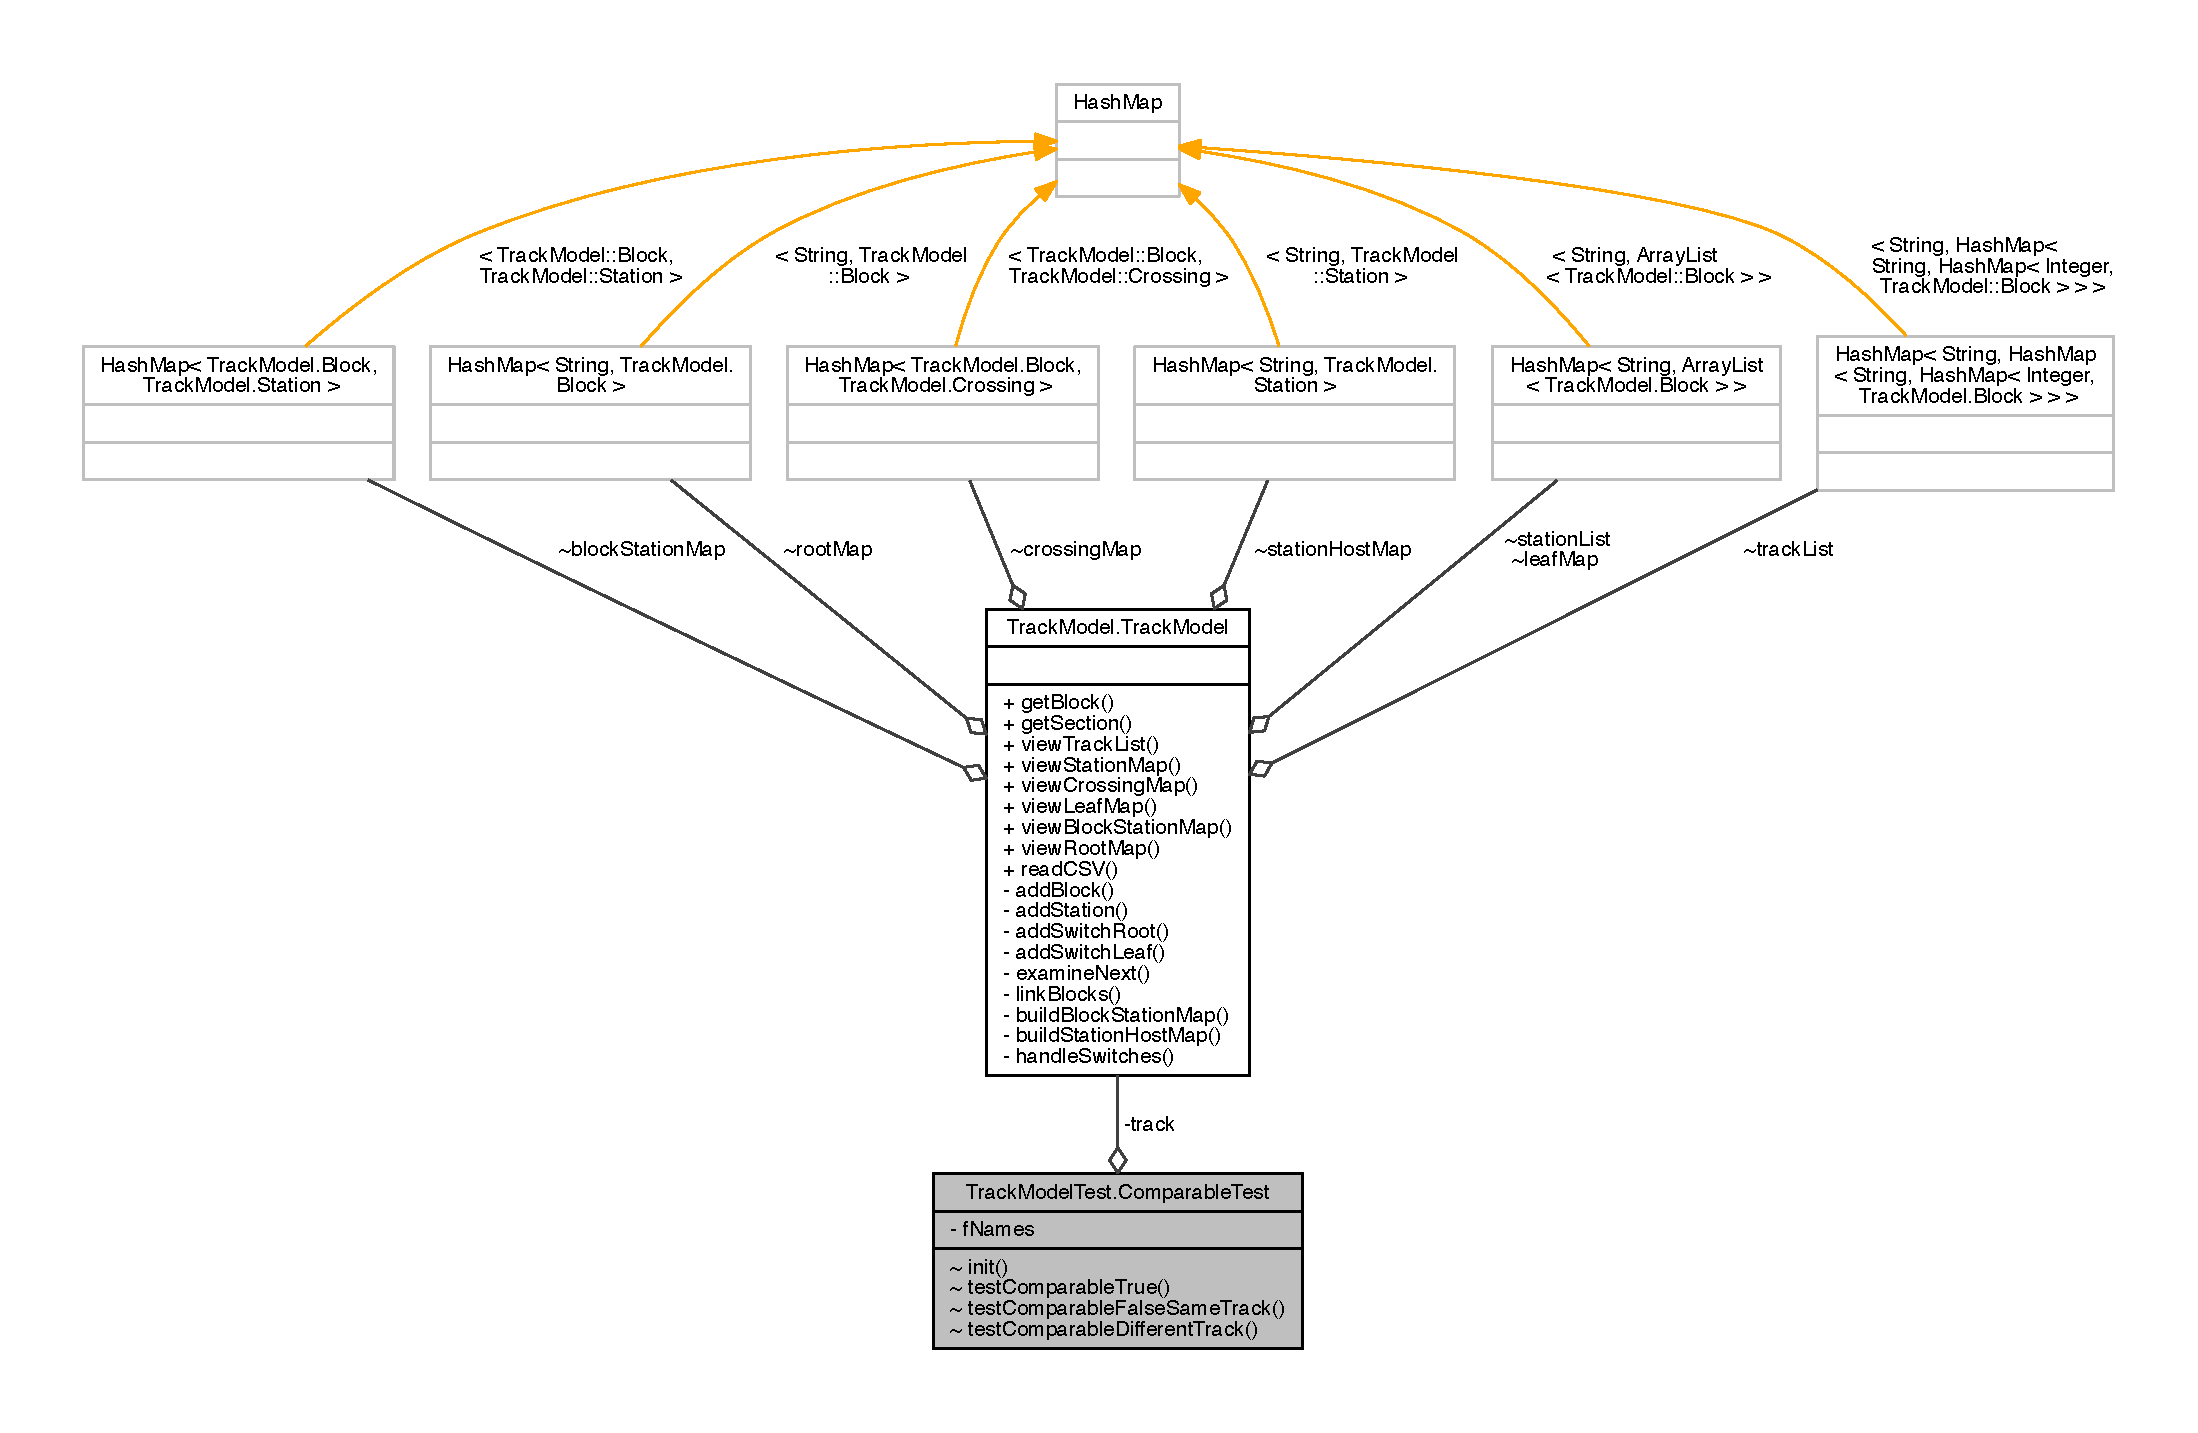
\includegraphics[width=350pt]{classTrackModelTest_1_1ComparableTest__coll__graph}
\end{center}
\end{figure}
\subsection*{Package Functions}
\begin{DoxyCompactItemize}
\item 
void \hyperlink{classTrackModelTest_1_1ComparableTest_a9f72a396557a4cf1b44c6186e123c1ac}{init} ()
\item 
void \hyperlink{classTrackModelTest_1_1ComparableTest_a907cb87775faa275c564a5dea19d7045}{test\+Comparable\+True} ()
\begin{DoxyCompactList}\small\item\em Test the comparable interface for a true result. \end{DoxyCompactList}\item 
void \hyperlink{classTrackModelTest_1_1ComparableTest_add7c697d3a7cfbaa93212cfc657b3d22}{test\+Comparable\+False\+Same\+Track} ()
\begin{DoxyCompactList}\small\item\em Test comparable false on the same line. \end{DoxyCompactList}\item 
void \hyperlink{classTrackModelTest_1_1ComparableTest_af0a95c84e6f6a63d42e110e6987e9b76}{test\+Comparable\+Different\+Track} ()
\begin{DoxyCompactList}\small\item\em Test comparable different tracks, same block+section. \end{DoxyCompactList}\end{DoxyCompactItemize}
\subsection*{Static Private Attributes}
\begin{DoxyCompactItemize}
\item 
static String \mbox{[}$\,$\mbox{]} \hyperlink{classTrackModelTest_1_1ComparableTest_a961e3115d8ca99145f56f318368f5582}{f\+Names} = \{\char`\"{}src/test/resources/redline.\+csv\char`\"{}, \char`\"{}src/test/resources/greenline.\+csv\char`\"{}\}
\item 
static \hyperlink{classTrackModel_1_1TrackModel}{Track\+Model} \hyperlink{classTrackModelTest_1_1ComparableTest_aecca898547ff5a1894e5739f9ba69124}{track}
\end{DoxyCompactItemize}


\subsection{Member Function Documentation}
\mbox{\Hypertarget{classTrackModelTest_1_1ComparableTest_a9f72a396557a4cf1b44c6186e123c1ac}\label{classTrackModelTest_1_1ComparableTest_a9f72a396557a4cf1b44c6186e123c1ac}} 
\index{Track\+Model\+Test\+::\+Comparable\+Test@{Track\+Model\+Test\+::\+Comparable\+Test}!init@{init}}
\index{init@{init}!Track\+Model\+Test\+::\+Comparable\+Test@{Track\+Model\+Test\+::\+Comparable\+Test}}
\subsubsection{\texorpdfstring{init()}{init()}}
{\footnotesize\ttfamily void Track\+Model\+Test.\+Comparable\+Test.\+init (\begin{DoxyParamCaption}{ }\end{DoxyParamCaption})\hspace{0.3cm}{\ttfamily [package]}}

\mbox{\Hypertarget{classTrackModelTest_1_1ComparableTest_af0a95c84e6f6a63d42e110e6987e9b76}\label{classTrackModelTest_1_1ComparableTest_af0a95c84e6f6a63d42e110e6987e9b76}} 
\index{Track\+Model\+Test\+::\+Comparable\+Test@{Track\+Model\+Test\+::\+Comparable\+Test}!test\+Comparable\+Different\+Track@{test\+Comparable\+Different\+Track}}
\index{test\+Comparable\+Different\+Track@{test\+Comparable\+Different\+Track}!Track\+Model\+Test\+::\+Comparable\+Test@{Track\+Model\+Test\+::\+Comparable\+Test}}
\subsubsection{\texorpdfstring{test\+Comparable\+Different\+Track()}{testComparableDifferentTrack()}}
{\footnotesize\ttfamily void Track\+Model\+Test.\+Comparable\+Test.\+test\+Comparable\+Different\+Track (\begin{DoxyParamCaption}{ }\end{DoxyParamCaption})\hspace{0.3cm}{\ttfamily [package]}}



Test comparable different tracks, same block+section. 

\mbox{\Hypertarget{classTrackModelTest_1_1ComparableTest_add7c697d3a7cfbaa93212cfc657b3d22}\label{classTrackModelTest_1_1ComparableTest_add7c697d3a7cfbaa93212cfc657b3d22}} 
\index{Track\+Model\+Test\+::\+Comparable\+Test@{Track\+Model\+Test\+::\+Comparable\+Test}!test\+Comparable\+False\+Same\+Track@{test\+Comparable\+False\+Same\+Track}}
\index{test\+Comparable\+False\+Same\+Track@{test\+Comparable\+False\+Same\+Track}!Track\+Model\+Test\+::\+Comparable\+Test@{Track\+Model\+Test\+::\+Comparable\+Test}}
\subsubsection{\texorpdfstring{test\+Comparable\+False\+Same\+Track()}{testComparableFalseSameTrack()}}
{\footnotesize\ttfamily void Track\+Model\+Test.\+Comparable\+Test.\+test\+Comparable\+False\+Same\+Track (\begin{DoxyParamCaption}{ }\end{DoxyParamCaption})\hspace{0.3cm}{\ttfamily [package]}}



Test comparable false on the same line. 

\mbox{\Hypertarget{classTrackModelTest_1_1ComparableTest_a907cb87775faa275c564a5dea19d7045}\label{classTrackModelTest_1_1ComparableTest_a907cb87775faa275c564a5dea19d7045}} 
\index{Track\+Model\+Test\+::\+Comparable\+Test@{Track\+Model\+Test\+::\+Comparable\+Test}!test\+Comparable\+True@{test\+Comparable\+True}}
\index{test\+Comparable\+True@{test\+Comparable\+True}!Track\+Model\+Test\+::\+Comparable\+Test@{Track\+Model\+Test\+::\+Comparable\+Test}}
\subsubsection{\texorpdfstring{test\+Comparable\+True()}{testComparableTrue()}}
{\footnotesize\ttfamily void Track\+Model\+Test.\+Comparable\+Test.\+test\+Comparable\+True (\begin{DoxyParamCaption}{ }\end{DoxyParamCaption})\hspace{0.3cm}{\ttfamily [package]}}



Test the comparable interface for a true result. 



\subsection{Member Data Documentation}
\mbox{\Hypertarget{classTrackModelTest_1_1ComparableTest_a961e3115d8ca99145f56f318368f5582}\label{classTrackModelTest_1_1ComparableTest_a961e3115d8ca99145f56f318368f5582}} 
\index{Track\+Model\+Test\+::\+Comparable\+Test@{Track\+Model\+Test\+::\+Comparable\+Test}!f\+Names@{f\+Names}}
\index{f\+Names@{f\+Names}!Track\+Model\+Test\+::\+Comparable\+Test@{Track\+Model\+Test\+::\+Comparable\+Test}}
\subsubsection{\texorpdfstring{f\+Names}{fNames}}
{\footnotesize\ttfamily String \mbox{[}$\,$\mbox{]} Track\+Model\+Test.\+Comparable\+Test.\+f\+Names = \{\char`\"{}src/test/resources/redline.\+csv\char`\"{}, \char`\"{}src/test/resources/greenline.\+csv\char`\"{}\}\hspace{0.3cm}{\ttfamily [static]}, {\ttfamily [private]}}

\mbox{\Hypertarget{classTrackModelTest_1_1ComparableTest_aecca898547ff5a1894e5739f9ba69124}\label{classTrackModelTest_1_1ComparableTest_aecca898547ff5a1894e5739f9ba69124}} 
\index{Track\+Model\+Test\+::\+Comparable\+Test@{Track\+Model\+Test\+::\+Comparable\+Test}!track@{track}}
\index{track@{track}!Track\+Model\+Test\+::\+Comparable\+Test@{Track\+Model\+Test\+::\+Comparable\+Test}}
\subsubsection{\texorpdfstring{track}{track}}
{\footnotesize\ttfamily \hyperlink{classTrackModel_1_1TrackModel}{Track\+Model} Track\+Model\+Test.\+Comparable\+Test.\+track\hspace{0.3cm}{\ttfamily [static]}, {\ttfamily [private]}}



The documentation for this class was generated from the following file\+:\begin{DoxyCompactItemize}
\item 
src/test/java/\+Track\+Model\+Test/\hyperlink{ComparableTest_8java}{Comparable\+Test.\+java}\end{DoxyCompactItemize}

\hypertarget{classCommonUIElements_1_1ConfirmationWindow}{}\section{Common\+U\+I\+Elements.\+Confirmation\+Window Class Reference}
\label{classCommonUIElements_1_1ConfirmationWindow}\index{Common\+U\+I\+Elements.\+Confirmation\+Window@{Common\+U\+I\+Elements.\+Confirmation\+Window}}


A window that displays a title and a message for a given amount of time, in seconds, and then closes.  




Inheritance diagram for Common\+U\+I\+Elements.\+Confirmation\+Window\+:
\nopagebreak
\begin{figure}[H]
\begin{center}
\leavevmode
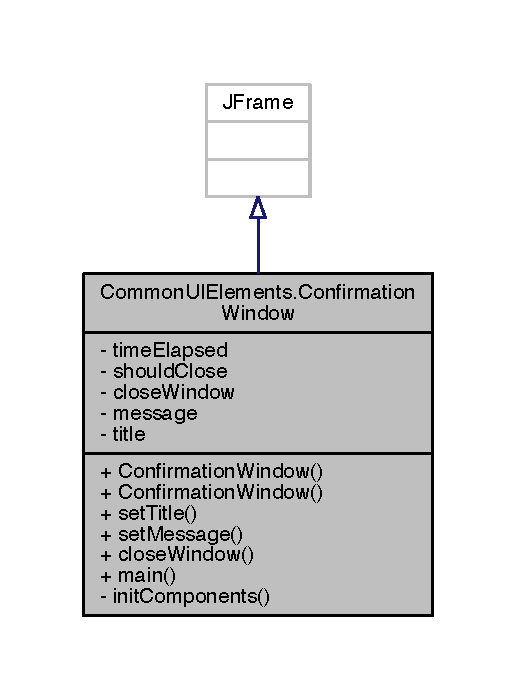
\includegraphics[width=248pt]{classCommonUIElements_1_1ConfirmationWindow__inherit__graph}
\end{center}
\end{figure}


Collaboration diagram for Common\+U\+I\+Elements.\+Confirmation\+Window\+:
\nopagebreak
\begin{figure}[H]
\begin{center}
\leavevmode
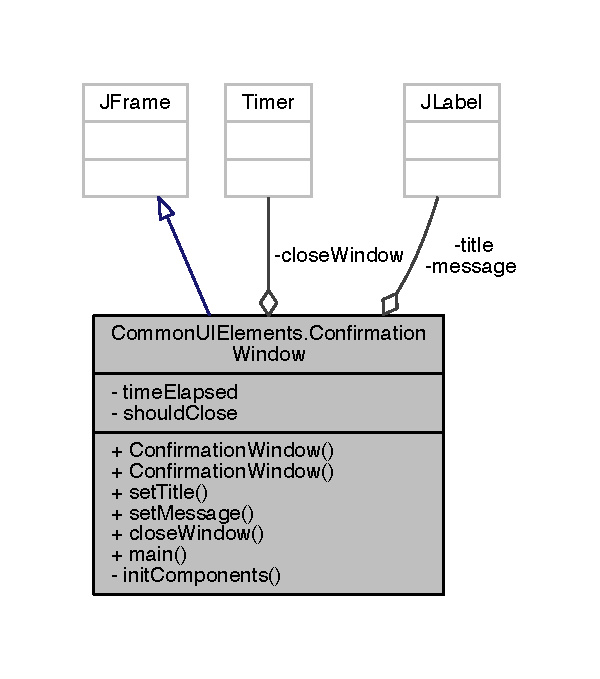
\includegraphics[width=288pt]{classCommonUIElements_1_1ConfirmationWindow__coll__graph}
\end{center}
\end{figure}
\subsection*{Public Member Functions}
\begin{DoxyCompactItemize}
\item 
\hyperlink{classCommonUIElements_1_1ConfirmationWindow_ae99ae36a3b34af52c80bfe2d404788c5}{Confirmation\+Window} ()
\begin{DoxyCompactList}\small\item\em Creates new form \hyperlink{classCommonUIElements_1_1ConfirmationWindow}{Confirmation\+Window}. \end{DoxyCompactList}\item 
\hyperlink{classCommonUIElements_1_1ConfirmationWindow_af0187cf6484465c088b4b1d49a345027}{Confirmation\+Window} (String \hyperlink{classCommonUIElements_1_1ConfirmationWindow_af03f991bc2c55d19a2507a54a20b6ab6}{title}, String \hyperlink{classCommonUIElements_1_1ConfirmationWindow_a5161ae2950ae7a12018c207a7d0ab1d5}{message}, int \hyperlink{classCommonUIElements_1_1ConfirmationWindow_ae9ba201fcec4a227a32aa9dd18f8224f}{should\+Close})
\begin{DoxyCompactList}\small\item\em Constructor that creates a \hyperlink{classCommonUIElements_1_1ConfirmationWindow}{Confirmation\+Window} with given title, message, and lifetime. \end{DoxyCompactList}\item 
void \hyperlink{classCommonUIElements_1_1ConfirmationWindow_a12e20697cbb522da6af910468f0df7bd}{set\+Title} (String \hyperlink{classCommonUIElements_1_1ConfirmationWindow_af03f991bc2c55d19a2507a54a20b6ab6}{title})
\begin{DoxyCompactList}\small\item\em Sets the title of the message. \end{DoxyCompactList}\item 
void \hyperlink{classCommonUIElements_1_1ConfirmationWindow_a3abf955dd0d33285a512f113800c77c5}{set\+Message} (String \hyperlink{classCommonUIElements_1_1ConfirmationWindow_a5161ae2950ae7a12018c207a7d0ab1d5}{message})
\begin{DoxyCompactList}\small\item\em Sets the message of window. \end{DoxyCompactList}\item 
void \hyperlink{classCommonUIElements_1_1ConfirmationWindow_ab3b4932646ddf67d77e6de3033d07176}{close\+Window} ()
\begin{DoxyCompactList}\small\item\em Closes the window by calling the dispose function. \end{DoxyCompactList}\end{DoxyCompactItemize}
\subsection*{Static Public Member Functions}
\begin{DoxyCompactItemize}
\item 
static void \hyperlink{classCommonUIElements_1_1ConfirmationWindow_a16def2d36e95c7be2b2bf3d435a4827c}{main} (String args\mbox{[}$\,$\mbox{]})
\end{DoxyCompactItemize}
\subsection*{Private Member Functions}
\begin{DoxyCompactItemize}
\item 
void \hyperlink{classCommonUIElements_1_1ConfirmationWindow_a1e0b5296df15f83d8e2fa52cc345e5a1}{init\+Components} ()
\begin{DoxyCompactList}\small\item\em This method is called from within the constructor to initialize the form. \end{DoxyCompactList}\end{DoxyCompactItemize}
\subsection*{Private Attributes}
\begin{DoxyCompactItemize}
\item 
int \hyperlink{classCommonUIElements_1_1ConfirmationWindow_a74e97a157709ec31ca3f48ff124c210c}{time\+Elapsed} = 0
\begin{DoxyCompactList}\small\item\em How much time, in seconds, the window how been open for. \end{DoxyCompactList}\item 
int \hyperlink{classCommonUIElements_1_1ConfirmationWindow_ae9ba201fcec4a227a32aa9dd18f8224f}{should\+Close}
\begin{DoxyCompactList}\small\item\em How long, in seconds, the window should stay open before closing. \end{DoxyCompactList}\item 
Timer \hyperlink{classCommonUIElements_1_1ConfirmationWindow_afaaac166e2198a99551498421b1759ff}{close\+Window}
\begin{DoxyCompactList}\small\item\em Timer used to keep track of lifetime of the window. \end{DoxyCompactList}\item 
javax.\+swing.\+J\+Label \hyperlink{classCommonUIElements_1_1ConfirmationWindow_a5161ae2950ae7a12018c207a7d0ab1d5}{message}
\item 
javax.\+swing.\+J\+Label \hyperlink{classCommonUIElements_1_1ConfirmationWindow_af03f991bc2c55d19a2507a54a20b6ab6}{title}
\end{DoxyCompactItemize}


\subsection{Detailed Description}
A window that displays a title and a message for a given amount of time, in seconds, and then closes. 

\begin{DoxyAuthor}{Author}
Andrew Lendacky 
\end{DoxyAuthor}


\subsection{Constructor \& Destructor Documentation}
\mbox{\Hypertarget{classCommonUIElements_1_1ConfirmationWindow_ae99ae36a3b34af52c80bfe2d404788c5}\label{classCommonUIElements_1_1ConfirmationWindow_ae99ae36a3b34af52c80bfe2d404788c5}} 
\index{Common\+U\+I\+Elements\+::\+Confirmation\+Window@{Common\+U\+I\+Elements\+::\+Confirmation\+Window}!Confirmation\+Window@{Confirmation\+Window}}
\index{Confirmation\+Window@{Confirmation\+Window}!Common\+U\+I\+Elements\+::\+Confirmation\+Window@{Common\+U\+I\+Elements\+::\+Confirmation\+Window}}
\subsubsection{\texorpdfstring{Confirmation\+Window()}{ConfirmationWindow()}\hspace{0.1cm}{\footnotesize\ttfamily [1/2]}}
{\footnotesize\ttfamily Common\+U\+I\+Elements.\+Confirmation\+Window.\+Confirmation\+Window (\begin{DoxyParamCaption}{ }\end{DoxyParamCaption})}



Creates new form \hyperlink{classCommonUIElements_1_1ConfirmationWindow}{Confirmation\+Window}. 

\mbox{\Hypertarget{classCommonUIElements_1_1ConfirmationWindow_af0187cf6484465c088b4b1d49a345027}\label{classCommonUIElements_1_1ConfirmationWindow_af0187cf6484465c088b4b1d49a345027}} 
\index{Common\+U\+I\+Elements\+::\+Confirmation\+Window@{Common\+U\+I\+Elements\+::\+Confirmation\+Window}!Confirmation\+Window@{Confirmation\+Window}}
\index{Confirmation\+Window@{Confirmation\+Window}!Common\+U\+I\+Elements\+::\+Confirmation\+Window@{Common\+U\+I\+Elements\+::\+Confirmation\+Window}}
\subsubsection{\texorpdfstring{Confirmation\+Window()}{ConfirmationWindow()}\hspace{0.1cm}{\footnotesize\ttfamily [2/2]}}
{\footnotesize\ttfamily Common\+U\+I\+Elements.\+Confirmation\+Window.\+Confirmation\+Window (\begin{DoxyParamCaption}\item[{String}]{title,  }\item[{String}]{message,  }\item[{int}]{should\+Close }\end{DoxyParamCaption})}



Constructor that creates a \hyperlink{classCommonUIElements_1_1ConfirmationWindow}{Confirmation\+Window} with given title, message, and lifetime. 


\begin{DoxyParams}{Parameters}
{\em title} & the title for the message. \\
\hline
{\em message} & the message. \\
\hline
{\em should\+Close} & how long the window should stay open for. \\
\hline
\end{DoxyParams}


\subsection{Member Function Documentation}
\mbox{\Hypertarget{classCommonUIElements_1_1ConfirmationWindow_ab3b4932646ddf67d77e6de3033d07176}\label{classCommonUIElements_1_1ConfirmationWindow_ab3b4932646ddf67d77e6de3033d07176}} 
\index{Common\+U\+I\+Elements\+::\+Confirmation\+Window@{Common\+U\+I\+Elements\+::\+Confirmation\+Window}!close\+Window@{close\+Window}}
\index{close\+Window@{close\+Window}!Common\+U\+I\+Elements\+::\+Confirmation\+Window@{Common\+U\+I\+Elements\+::\+Confirmation\+Window}}
\subsubsection{\texorpdfstring{close\+Window()}{closeWindow()}}
{\footnotesize\ttfamily void Common\+U\+I\+Elements.\+Confirmation\+Window.\+close\+Window (\begin{DoxyParamCaption}{ }\end{DoxyParamCaption})}



Closes the window by calling the dispose function. 

\mbox{\Hypertarget{classCommonUIElements_1_1ConfirmationWindow_a1e0b5296df15f83d8e2fa52cc345e5a1}\label{classCommonUIElements_1_1ConfirmationWindow_a1e0b5296df15f83d8e2fa52cc345e5a1}} 
\index{Common\+U\+I\+Elements\+::\+Confirmation\+Window@{Common\+U\+I\+Elements\+::\+Confirmation\+Window}!init\+Components@{init\+Components}}
\index{init\+Components@{init\+Components}!Common\+U\+I\+Elements\+::\+Confirmation\+Window@{Common\+U\+I\+Elements\+::\+Confirmation\+Window}}
\subsubsection{\texorpdfstring{init\+Components()}{initComponents()}}
{\footnotesize\ttfamily void Common\+U\+I\+Elements.\+Confirmation\+Window.\+init\+Components (\begin{DoxyParamCaption}{ }\end{DoxyParamCaption})\hspace{0.3cm}{\ttfamily [private]}}



This method is called from within the constructor to initialize the form. 

W\+A\+R\+N\+I\+NG\+: Do N\+OT modify this code. The content of this method is always regenerated by the Form Editor. \mbox{\Hypertarget{classCommonUIElements_1_1ConfirmationWindow_a16def2d36e95c7be2b2bf3d435a4827c}\label{classCommonUIElements_1_1ConfirmationWindow_a16def2d36e95c7be2b2bf3d435a4827c}} 
\index{Common\+U\+I\+Elements\+::\+Confirmation\+Window@{Common\+U\+I\+Elements\+::\+Confirmation\+Window}!main@{main}}
\index{main@{main}!Common\+U\+I\+Elements\+::\+Confirmation\+Window@{Common\+U\+I\+Elements\+::\+Confirmation\+Window}}
\subsubsection{\texorpdfstring{main()}{main()}}
{\footnotesize\ttfamily static void Common\+U\+I\+Elements.\+Confirmation\+Window.\+main (\begin{DoxyParamCaption}\item[{String}]{args\mbox{[}$\,$\mbox{]} }\end{DoxyParamCaption})\hspace{0.3cm}{\ttfamily [static]}}


\begin{DoxyParams}{Parameters}
{\em args} & the command line arguments \\
\hline
\end{DoxyParams}
\mbox{\Hypertarget{classCommonUIElements_1_1ConfirmationWindow_a3abf955dd0d33285a512f113800c77c5}\label{classCommonUIElements_1_1ConfirmationWindow_a3abf955dd0d33285a512f113800c77c5}} 
\index{Common\+U\+I\+Elements\+::\+Confirmation\+Window@{Common\+U\+I\+Elements\+::\+Confirmation\+Window}!set\+Message@{set\+Message}}
\index{set\+Message@{set\+Message}!Common\+U\+I\+Elements\+::\+Confirmation\+Window@{Common\+U\+I\+Elements\+::\+Confirmation\+Window}}
\subsubsection{\texorpdfstring{set\+Message()}{setMessage()}}
{\footnotesize\ttfamily void Common\+U\+I\+Elements.\+Confirmation\+Window.\+set\+Message (\begin{DoxyParamCaption}\item[{String}]{message }\end{DoxyParamCaption})}



Sets the message of window. 


\begin{DoxyParams}{Parameters}
{\em message} & the message you want the window to display. \\
\hline
\end{DoxyParams}
\mbox{\Hypertarget{classCommonUIElements_1_1ConfirmationWindow_a12e20697cbb522da6af910468f0df7bd}\label{classCommonUIElements_1_1ConfirmationWindow_a12e20697cbb522da6af910468f0df7bd}} 
\index{Common\+U\+I\+Elements\+::\+Confirmation\+Window@{Common\+U\+I\+Elements\+::\+Confirmation\+Window}!set\+Title@{set\+Title}}
\index{set\+Title@{set\+Title}!Common\+U\+I\+Elements\+::\+Confirmation\+Window@{Common\+U\+I\+Elements\+::\+Confirmation\+Window}}
\subsubsection{\texorpdfstring{set\+Title()}{setTitle()}}
{\footnotesize\ttfamily void Common\+U\+I\+Elements.\+Confirmation\+Window.\+set\+Title (\begin{DoxyParamCaption}\item[{String}]{title }\end{DoxyParamCaption})}



Sets the title of the message. 


\begin{DoxyParams}{Parameters}
{\em title} & the title of the message. \\
\hline
\end{DoxyParams}


\subsection{Member Data Documentation}
\mbox{\Hypertarget{classCommonUIElements_1_1ConfirmationWindow_afaaac166e2198a99551498421b1759ff}\label{classCommonUIElements_1_1ConfirmationWindow_afaaac166e2198a99551498421b1759ff}} 
\index{Common\+U\+I\+Elements\+::\+Confirmation\+Window@{Common\+U\+I\+Elements\+::\+Confirmation\+Window}!close\+Window@{close\+Window}}
\index{close\+Window@{close\+Window}!Common\+U\+I\+Elements\+::\+Confirmation\+Window@{Common\+U\+I\+Elements\+::\+Confirmation\+Window}}
\subsubsection{\texorpdfstring{close\+Window}{closeWindow}}
{\footnotesize\ttfamily Timer Common\+U\+I\+Elements.\+Confirmation\+Window.\+close\+Window\hspace{0.3cm}{\ttfamily [private]}}

{\bfseries Initial value\+:}
\begin{DoxyCode}
= \textcolor{keyword}{new} Timer(1000, \textcolor{keyword}{new} ActionListener()\{
       
        \textcolor{keyword}{public} \textcolor{keywordtype}{void} actionPerformed(ActionEvent e) \{
            \hyperlink{classCommonUIElements_1_1ConfirmationWindow_a74e97a157709ec31ca3f48ff124c210c}{timeElapsed}++; 
           
            \textcolor{keywordflow}{if} (\hyperlink{classCommonUIElements_1_1ConfirmationWindow_a74e97a157709ec31ca3f48ff124c210c}{timeElapsed} == 1)\{
                
                System.out.println(\textcolor{stringliteral}{"Closing Window"}); 
                \hyperlink{classCommonUIElements_1_1ConfirmationWindow_ab3b4932646ddf67d77e6de3033d07176}{closeWindow}(); 
                \hyperlink{classCommonUIElements_1_1ConfirmationWindow_ab3b4932646ddf67d77e6de3033d07176}{closeWindow}.stop();
            \}       
        \}   
        \})
\end{DoxyCode}


Timer used to keep track of lifetime of the window. 

This timer will close the window once the \textquotesingle{}time\+Elapsed\textquotesingle{} reaches the \textquotesingle{}should\+Close\textquotesingle{} value. \mbox{\Hypertarget{classCommonUIElements_1_1ConfirmationWindow_a5161ae2950ae7a12018c207a7d0ab1d5}\label{classCommonUIElements_1_1ConfirmationWindow_a5161ae2950ae7a12018c207a7d0ab1d5}} 
\index{Common\+U\+I\+Elements\+::\+Confirmation\+Window@{Common\+U\+I\+Elements\+::\+Confirmation\+Window}!message@{message}}
\index{message@{message}!Common\+U\+I\+Elements\+::\+Confirmation\+Window@{Common\+U\+I\+Elements\+::\+Confirmation\+Window}}
\subsubsection{\texorpdfstring{message}{message}}
{\footnotesize\ttfamily javax.\+swing.\+J\+Label Common\+U\+I\+Elements.\+Confirmation\+Window.\+message\hspace{0.3cm}{\ttfamily [private]}}

\mbox{\Hypertarget{classCommonUIElements_1_1ConfirmationWindow_ae9ba201fcec4a227a32aa9dd18f8224f}\label{classCommonUIElements_1_1ConfirmationWindow_ae9ba201fcec4a227a32aa9dd18f8224f}} 
\index{Common\+U\+I\+Elements\+::\+Confirmation\+Window@{Common\+U\+I\+Elements\+::\+Confirmation\+Window}!should\+Close@{should\+Close}}
\index{should\+Close@{should\+Close}!Common\+U\+I\+Elements\+::\+Confirmation\+Window@{Common\+U\+I\+Elements\+::\+Confirmation\+Window}}
\subsubsection{\texorpdfstring{should\+Close}{shouldClose}}
{\footnotesize\ttfamily int Common\+U\+I\+Elements.\+Confirmation\+Window.\+should\+Close\hspace{0.3cm}{\ttfamily [private]}}



How long, in seconds, the window should stay open before closing. 

\mbox{\Hypertarget{classCommonUIElements_1_1ConfirmationWindow_a74e97a157709ec31ca3f48ff124c210c}\label{classCommonUIElements_1_1ConfirmationWindow_a74e97a157709ec31ca3f48ff124c210c}} 
\index{Common\+U\+I\+Elements\+::\+Confirmation\+Window@{Common\+U\+I\+Elements\+::\+Confirmation\+Window}!time\+Elapsed@{time\+Elapsed}}
\index{time\+Elapsed@{time\+Elapsed}!Common\+U\+I\+Elements\+::\+Confirmation\+Window@{Common\+U\+I\+Elements\+::\+Confirmation\+Window}}
\subsubsection{\texorpdfstring{time\+Elapsed}{timeElapsed}}
{\footnotesize\ttfamily int Common\+U\+I\+Elements.\+Confirmation\+Window.\+time\+Elapsed = 0\hspace{0.3cm}{\ttfamily [private]}}



How much time, in seconds, the window how been open for. 

\mbox{\Hypertarget{classCommonUIElements_1_1ConfirmationWindow_af03f991bc2c55d19a2507a54a20b6ab6}\label{classCommonUIElements_1_1ConfirmationWindow_af03f991bc2c55d19a2507a54a20b6ab6}} 
\index{Common\+U\+I\+Elements\+::\+Confirmation\+Window@{Common\+U\+I\+Elements\+::\+Confirmation\+Window}!title@{title}}
\index{title@{title}!Common\+U\+I\+Elements\+::\+Confirmation\+Window@{Common\+U\+I\+Elements\+::\+Confirmation\+Window}}
\subsubsection{\texorpdfstring{title}{title}}
{\footnotesize\ttfamily javax.\+swing.\+J\+Label Common\+U\+I\+Elements.\+Confirmation\+Window.\+title\hspace{0.3cm}{\ttfamily [private]}}



The documentation for this class was generated from the following file\+:\begin{DoxyCompactItemize}
\item 
src/main/java/\+Common\+U\+I\+Elements/\hyperlink{ConfirmationWindow_8java}{Confirmation\+Window.\+java}\end{DoxyCompactItemize}

\hypertarget{classTrackModel_1_1Crossing}{}\section{Track\+Model.\+Crossing Class Reference}
\label{classTrackModel_1_1Crossing}\index{Track\+Model.\+Crossing@{Track\+Model.\+Crossing}}


Collaboration diagram for Track\+Model.\+Crossing\+:
\nopagebreak
\begin{figure}[H]
\begin{center}
\leavevmode
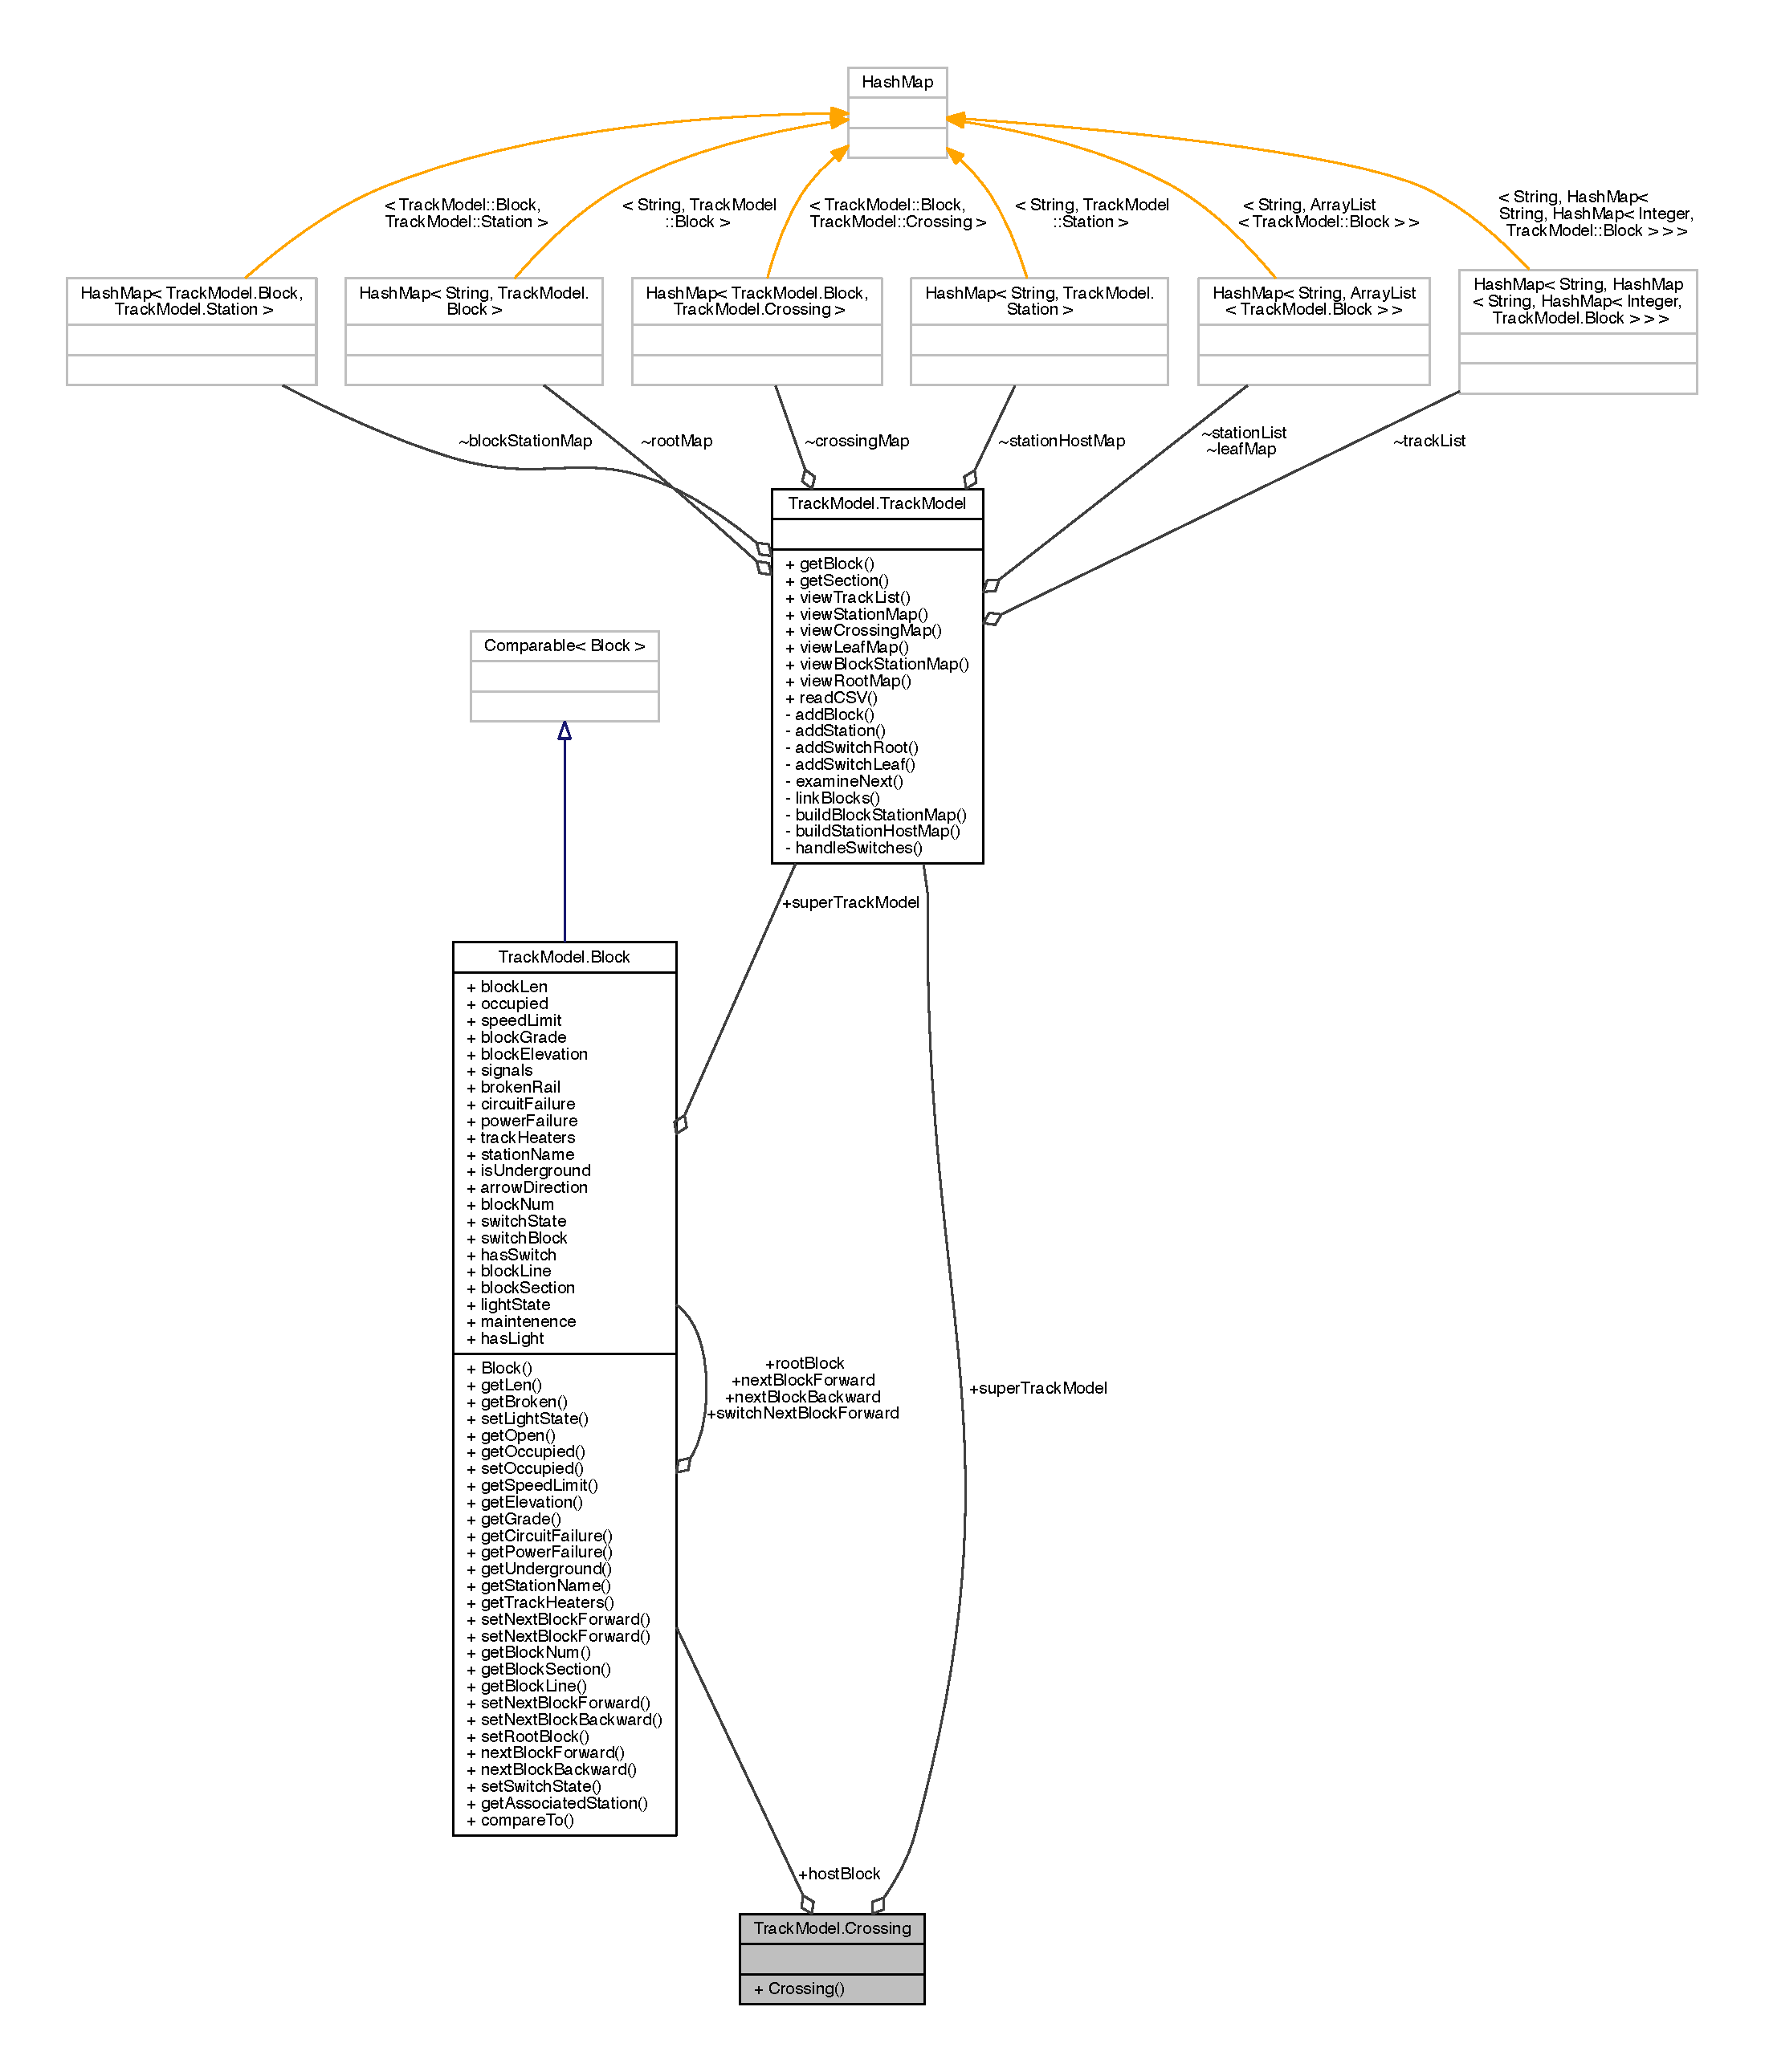
\includegraphics[width=350pt]{classTrackModel_1_1Crossing__coll__graph}
\end{center}
\end{figure}
\subsection*{Public Member Functions}
\begin{DoxyCompactItemize}
\item 
\hyperlink{classTrackModel_1_1Crossing_ab23fc0855d053936d68d367ce898d152}{Crossing} (\hyperlink{classTrackModel_1_1Block}{Block} \hyperlink{classTrackModel_1_1Crossing_a1e9bc8acd2681fa0c85cf43cfec99368}{host\+Block})
\end{DoxyCompactItemize}
\subsection*{Public Attributes}
\begin{DoxyCompactItemize}
\item 
\hyperlink{classTrackModel_1_1Block}{Block} \hyperlink{classTrackModel_1_1Crossing_a1e9bc8acd2681fa0c85cf43cfec99368}{host\+Block}
\item 
\hyperlink{classTrackModel_1_1TrackModel}{Track\+Model} \hyperlink{classTrackModel_1_1Crossing_af353edaf8c1d5f5cad24ffc45f3370e4}{super\+Track\+Model}
\end{DoxyCompactItemize}


\subsection{Constructor \& Destructor Documentation}
\mbox{\Hypertarget{classTrackModel_1_1Crossing_ab23fc0855d053936d68d367ce898d152}\label{classTrackModel_1_1Crossing_ab23fc0855d053936d68d367ce898d152}} 
\index{Track\+Model\+::\+Crossing@{Track\+Model\+::\+Crossing}!Crossing@{Crossing}}
\index{Crossing@{Crossing}!Track\+Model\+::\+Crossing@{Track\+Model\+::\+Crossing}}
\subsubsection{\texorpdfstring{Crossing()}{Crossing()}}
{\footnotesize\ttfamily Track\+Model.\+Crossing.\+Crossing (\begin{DoxyParamCaption}\item[{\hyperlink{classTrackModel_1_1Block}{Block}}]{host\+Block }\end{DoxyParamCaption})}



\subsection{Member Data Documentation}
\mbox{\Hypertarget{classTrackModel_1_1Crossing_a1e9bc8acd2681fa0c85cf43cfec99368}\label{classTrackModel_1_1Crossing_a1e9bc8acd2681fa0c85cf43cfec99368}} 
\index{Track\+Model\+::\+Crossing@{Track\+Model\+::\+Crossing}!host\+Block@{host\+Block}}
\index{host\+Block@{host\+Block}!Track\+Model\+::\+Crossing@{Track\+Model\+::\+Crossing}}
\subsubsection{\texorpdfstring{host\+Block}{hostBlock}}
{\footnotesize\ttfamily \hyperlink{classTrackModel_1_1Block}{Block} Track\+Model.\+Crossing.\+host\+Block}

\mbox{\Hypertarget{classTrackModel_1_1Crossing_af353edaf8c1d5f5cad24ffc45f3370e4}\label{classTrackModel_1_1Crossing_af353edaf8c1d5f5cad24ffc45f3370e4}} 
\index{Track\+Model\+::\+Crossing@{Track\+Model\+::\+Crossing}!super\+Track\+Model@{super\+Track\+Model}}
\index{super\+Track\+Model@{super\+Track\+Model}!Track\+Model\+::\+Crossing@{Track\+Model\+::\+Crossing}}
\subsubsection{\texorpdfstring{super\+Track\+Model}{superTrackModel}}
{\footnotesize\ttfamily \hyperlink{classTrackModel_1_1TrackModel}{Track\+Model} Track\+Model.\+Crossing.\+super\+Track\+Model}



The documentation for this class was generated from the following file\+:\begin{DoxyCompactItemize}
\item 
src/main/java/\+Track\+Model/\hyperlink{Crossing_8java}{Crossing.\+java}\end{DoxyCompactItemize}

\hypertarget{classCTC__gui}{}\section{C\+T\+C\+\_\+gui Class Reference}
\label{classCTC__gui}\index{C\+T\+C\+\_\+gui@{C\+T\+C\+\_\+gui}}


Collaboration diagram for C\+T\+C\+\_\+gui\+:
\nopagebreak
\begin{figure}[H]
\begin{center}
\leavevmode
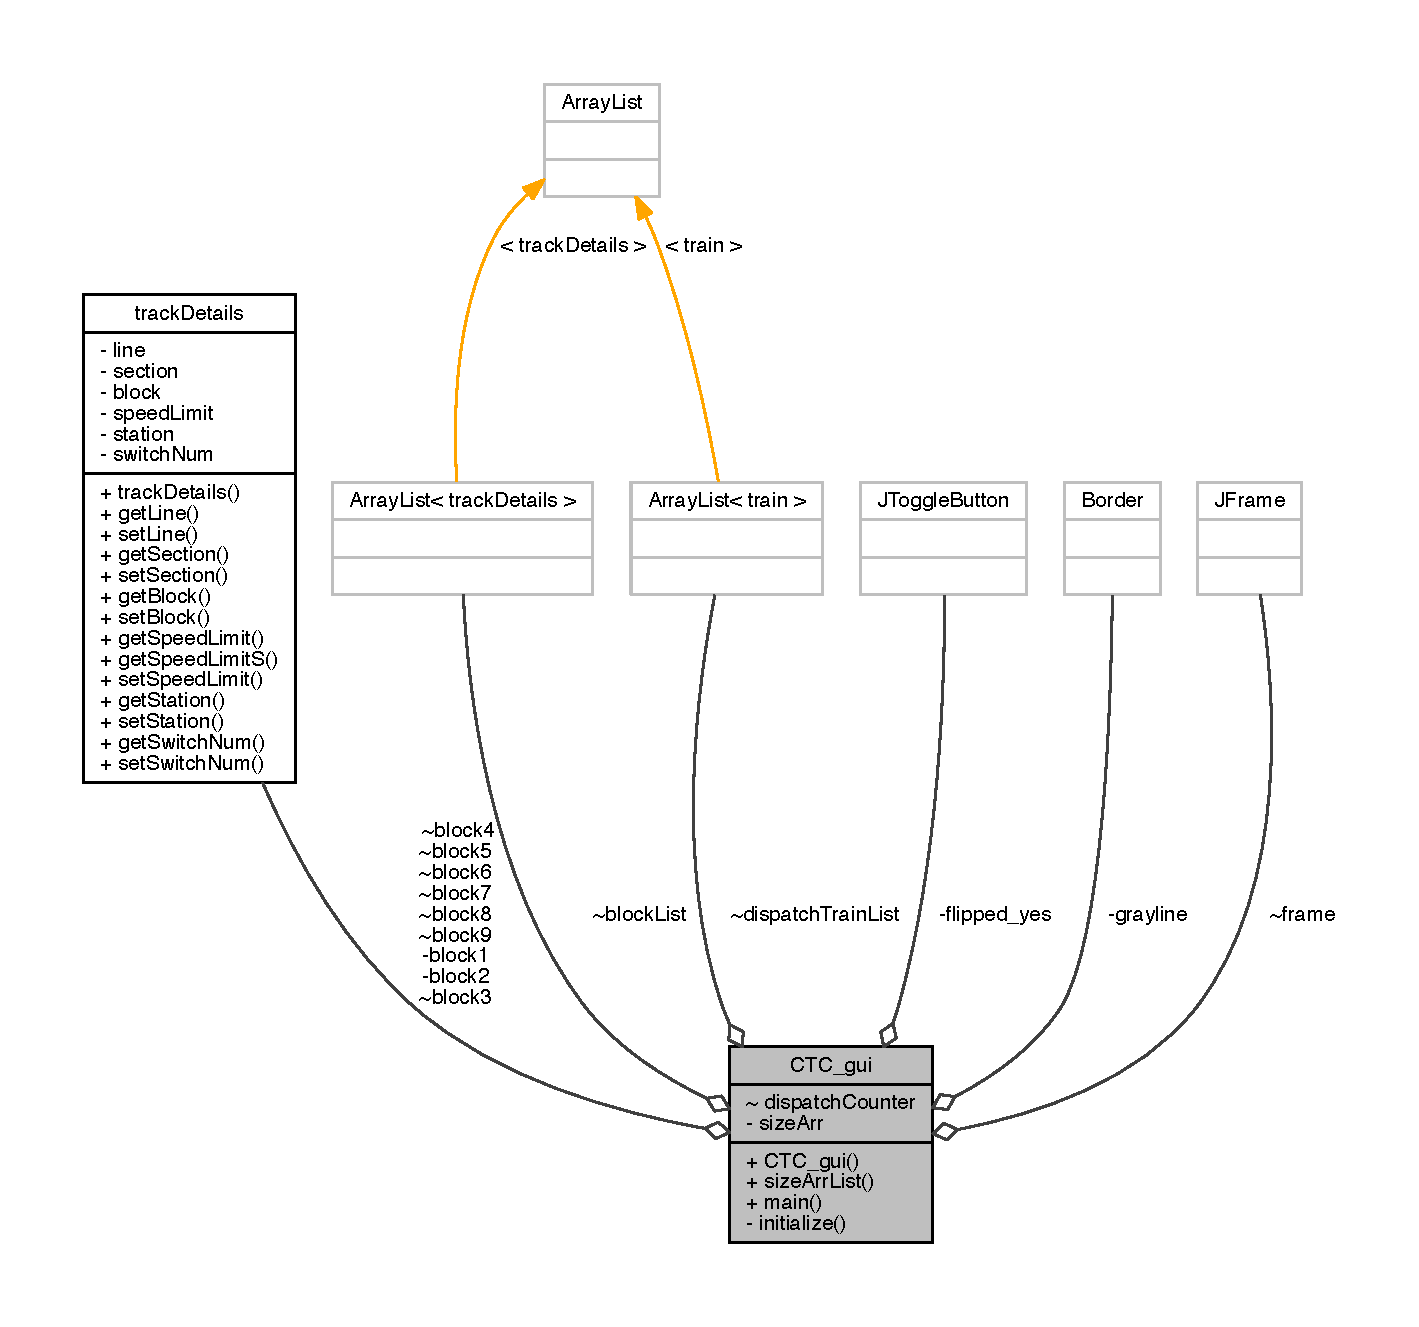
\includegraphics[width=350pt]{classCTC__gui__coll__graph}
\end{center}
\end{figure}
\subsection*{Public Member Functions}
\begin{DoxyCompactItemize}
\item 
\hyperlink{classCTC__gui_a2e77261492fe815cec81ff396aaeb5f9}{C\+T\+C\+\_\+gui} ()
\begin{DoxyCompactList}\small\item\em Create the application. \end{DoxyCompactList}\item 
int \hyperlink{classCTC__gui_a985c2650c57b753dcc510ebccc169c63}{size\+Arr\+List} (Array\+List$<$ \hyperlink{classtrain}{train} $>$ train\+List)
\end{DoxyCompactItemize}
\subsection*{Static Public Member Functions}
\begin{DoxyCompactItemize}
\item 
static void \hyperlink{classCTC__gui_ad97ec7b3c189ca4cb572df0156b9a330}{main} (String\mbox{[}$\,$\mbox{]} args)  throws Class\+Not\+Found\+Exception, Instantiation\+Exception, Illegal\+Access\+Exception, Unsupported\+Look\+And\+Feel\+Exception 
\begin{DoxyCompactList}\small\item\em Launch the application. \end{DoxyCompactList}\end{DoxyCompactItemize}
\subsection*{Package Attributes}
\begin{DoxyCompactItemize}
\item 
J\+Frame \hyperlink{classCTC__gui_aac594c597dd95e3dbdda3050143a62f1}{frame}
\end{DoxyCompactItemize}
\subsection*{Static Package Attributes}
\begin{DoxyCompactItemize}
\item 
static Array\+List$<$ \hyperlink{classtrain}{train} $>$ \hyperlink{classCTC__gui_ab5fa6fd520ef7d0ef6e08fa07699d208}{dispatch\+Train\+List} = new Array\+List$<$\hyperlink{classtrain}{train}$>$()
\item 
static Integer \hyperlink{classCTC__gui_ac03f22e602d0114ee24385cee260d39f}{dispatch\+Counter} = 0
\item 
static \hyperlink{classtrackDetails}{track\+Details} \hyperlink{classCTC__gui_ac0d6e738f3b1462abd7b962bd58d82ea}{block3} = new \hyperlink{classtrackDetails}{track\+Details}(\char`\"{}Red\char`\"{}, \char`\"{}A\char`\"{}, 3, 24.\+8548, \char`\"{}\char`\"{}, \char`\"{}\char`\"{})
\item 
static \hyperlink{classtrackDetails}{track\+Details} \hyperlink{classCTC__gui_a15dab97be71f3b0198ec1e25f76408fe}{block4} = new \hyperlink{classtrackDetails}{track\+Details}(\char`\"{}Red\char`\"{}, \char`\"{}B\char`\"{}, 4, 24.\+8548, \char`\"{}\char`\"{}, \char`\"{}\char`\"{})
\item 
static \hyperlink{classtrackDetails}{track\+Details} \hyperlink{classCTC__gui_a8a1217dd7fb5da4f4179f554d06854d4}{block5} = new \hyperlink{classtrackDetails}{track\+Details}(\char`\"{}Red\char`\"{}, \char`\"{}B\char`\"{}, 5, 24.\+8548, \char`\"{}\char`\"{}, \char`\"{}\char`\"{})
\item 
static \hyperlink{classtrackDetails}{track\+Details} \hyperlink{classCTC__gui_a54becfe14761bd88f15a1757245422c6}{block6} = new \hyperlink{classtrackDetails}{track\+Details}(\char`\"{}Red\char`\"{}, \char`\"{}B\char`\"{}, 6, 24.\+8548, \char`\"{}\char`\"{}, \char`\"{}\char`\"{})
\item 
static \hyperlink{classtrackDetails}{track\+Details} \hyperlink{classCTC__gui_a5b98f4aed52daa3a53ebb68a3930756e}{block7} = new \hyperlink{classtrackDetails}{track\+Details}(\char`\"{}Red\char`\"{}, \char`\"{}C\char`\"{}, 7, 24.\+8548, \char`\"{}Shadyside\char`\"{}, \char`\"{}\char`\"{})
\item 
static \hyperlink{classtrackDetails}{track\+Details} \hyperlink{classCTC__gui_a2fbaa1b3920a22fb3180b607abb15d78}{block8} = new \hyperlink{classtrackDetails}{track\+Details}(\char`\"{}Red\char`\"{}, \char`\"{}C\char`\"{}, 8, 24.\+8548, \char`\"{}\char`\"{}, \char`\"{}\char`\"{})
\item 
static \hyperlink{classtrackDetails}{track\+Details} \hyperlink{classCTC__gui_ad71b4889f6be57834e8dffb5a0e5ed37}{block9} = new \hyperlink{classtrackDetails}{track\+Details}(\char`\"{}Red\char`\"{}, \char`\"{}C\char`\"{}, 9, 24.\+8548, \char`\"{}Yard\char`\"{}, \char`\"{}12\char`\"{})
\item 
static Array\+List$<$ \hyperlink{classtrackDetails}{track\+Details} $>$ \hyperlink{classCTC__gui_a64af0234646b1a791a6dd3b5e4a77950}{block\+List} = new Array\+List$<$\hyperlink{classtrackDetails}{track\+Details}$>$()
\end{DoxyCompactItemize}
\subsection*{Private Member Functions}
\begin{DoxyCompactItemize}
\item 
void \hyperlink{classCTC__gui_af8298a2936080671d12fc6c0ca5dd7a3}{initialize} ()
\begin{DoxyCompactList}\small\item\em Initialize the contents of the frame. \end{DoxyCompactList}\end{DoxyCompactItemize}
\subsection*{Private Attributes}
\begin{DoxyCompactItemize}
\item 
Border \hyperlink{classCTC__gui_abc2e3bfbf18d4e85c0ad27a18af06a62}{grayline}
\item 
J\+Toggle\+Button \hyperlink{classCTC__gui_ac1dbe678dae57ea63c6a647b0e6a10df}{flipped\+\_\+yes}
\item 
int \hyperlink{classCTC__gui_a1394f1231e8fda2c6437d072e28d1da2}{size\+Arr} = 0
\item 
\hyperlink{classtrackDetails}{track\+Details} \hyperlink{classCTC__gui_a9f323c3477f61193b3e87c047eed84a7}{block1} = new \hyperlink{classtrackDetails}{track\+Details}(\char`\"{}Red\char`\"{}, \char`\"{}A\char`\"{}, 1, 24.\+8548, \char`\"{}\char`\"{}, \char`\"{}6\char`\"{})
\item 
\hyperlink{classtrackDetails}{track\+Details} \hyperlink{classCTC__gui_af19fcf01d102c99e349cba43ac13a3a3}{block2} = new \hyperlink{classtrackDetails}{track\+Details}(\char`\"{}Red\char`\"{}, \char`\"{}A\char`\"{}, 2, 24.\+8548, \char`\"{}\char`\"{}, \char`\"{}\char`\"{})
\end{DoxyCompactItemize}


\subsection{Constructor \& Destructor Documentation}
\mbox{\Hypertarget{classCTC__gui_a2e77261492fe815cec81ff396aaeb5f9}\label{classCTC__gui_a2e77261492fe815cec81ff396aaeb5f9}} 
\index{C\+T\+C\+\_\+gui@{C\+T\+C\+\_\+gui}!C\+T\+C\+\_\+gui@{C\+T\+C\+\_\+gui}}
\index{C\+T\+C\+\_\+gui@{C\+T\+C\+\_\+gui}!C\+T\+C\+\_\+gui@{C\+T\+C\+\_\+gui}}
\subsubsection{\texorpdfstring{C\+T\+C\+\_\+gui()}{CTC\_gui()}}
{\footnotesize\ttfamily C\+T\+C\+\_\+gui.\+C\+T\+C\+\_\+gui (\begin{DoxyParamCaption}{ }\end{DoxyParamCaption})}



Create the application. 



\subsection{Member Function Documentation}
\mbox{\Hypertarget{classCTC__gui_af8298a2936080671d12fc6c0ca5dd7a3}\label{classCTC__gui_af8298a2936080671d12fc6c0ca5dd7a3}} 
\index{C\+T\+C\+\_\+gui@{C\+T\+C\+\_\+gui}!initialize@{initialize}}
\index{initialize@{initialize}!C\+T\+C\+\_\+gui@{C\+T\+C\+\_\+gui}}
\subsubsection{\texorpdfstring{initialize()}{initialize()}}
{\footnotesize\ttfamily void C\+T\+C\+\_\+gui.\+initialize (\begin{DoxyParamCaption}{ }\end{DoxyParamCaption})\hspace{0.3cm}{\ttfamily [private]}}



Initialize the contents of the frame. 

\mbox{\Hypertarget{classCTC__gui_ad97ec7b3c189ca4cb572df0156b9a330}\label{classCTC__gui_ad97ec7b3c189ca4cb572df0156b9a330}} 
\index{C\+T\+C\+\_\+gui@{C\+T\+C\+\_\+gui}!main@{main}}
\index{main@{main}!C\+T\+C\+\_\+gui@{C\+T\+C\+\_\+gui}}
\subsubsection{\texorpdfstring{main()}{main()}}
{\footnotesize\ttfamily static void C\+T\+C\+\_\+gui.\+main (\begin{DoxyParamCaption}\item[{String \mbox{[}$\,$\mbox{]}}]{args }\end{DoxyParamCaption}) throws Class\+Not\+Found\+Exception, Instantiation\+Exception, Illegal\+Access\+Exception, Unsupported\+Look\+And\+Feel\+Exception\hspace{0.3cm}{\ttfamily [static]}}



Launch the application. 


\begin{DoxyExceptions}{Exceptions}
{\em Unsupported\+Look\+And\+Feel\+Exception} & \\
\hline
{\em Illegal\+Access\+Exception} & \\
\hline
{\em Instantiation\+Exception} & \\
\hline
{\em Class\+Not\+Found\+Exception} & \\
\hline
\end{DoxyExceptions}
\mbox{\Hypertarget{classCTC__gui_a985c2650c57b753dcc510ebccc169c63}\label{classCTC__gui_a985c2650c57b753dcc510ebccc169c63}} 
\index{C\+T\+C\+\_\+gui@{C\+T\+C\+\_\+gui}!size\+Arr\+List@{size\+Arr\+List}}
\index{size\+Arr\+List@{size\+Arr\+List}!C\+T\+C\+\_\+gui@{C\+T\+C\+\_\+gui}}
\subsubsection{\texorpdfstring{size\+Arr\+List()}{sizeArrList()}}
{\footnotesize\ttfamily int C\+T\+C\+\_\+gui.\+size\+Arr\+List (\begin{DoxyParamCaption}\item[{Array\+List$<$ \hyperlink{classtrain}{train} $>$}]{train\+List }\end{DoxyParamCaption})}



\subsection{Member Data Documentation}
\mbox{\Hypertarget{classCTC__gui_a9f323c3477f61193b3e87c047eed84a7}\label{classCTC__gui_a9f323c3477f61193b3e87c047eed84a7}} 
\index{C\+T\+C\+\_\+gui@{C\+T\+C\+\_\+gui}!block1@{block1}}
\index{block1@{block1}!C\+T\+C\+\_\+gui@{C\+T\+C\+\_\+gui}}
\subsubsection{\texorpdfstring{block1}{block1}}
{\footnotesize\ttfamily \hyperlink{classtrackDetails}{track\+Details} C\+T\+C\+\_\+gui.\+block1 = new \hyperlink{classtrackDetails}{track\+Details}(\char`\"{}Red\char`\"{}, \char`\"{}A\char`\"{}, 1, 24.\+8548, \char`\"{}\char`\"{}, \char`\"{}6\char`\"{})\hspace{0.3cm}{\ttfamily [private]}}

\mbox{\Hypertarget{classCTC__gui_af19fcf01d102c99e349cba43ac13a3a3}\label{classCTC__gui_af19fcf01d102c99e349cba43ac13a3a3}} 
\index{C\+T\+C\+\_\+gui@{C\+T\+C\+\_\+gui}!block2@{block2}}
\index{block2@{block2}!C\+T\+C\+\_\+gui@{C\+T\+C\+\_\+gui}}
\subsubsection{\texorpdfstring{block2}{block2}}
{\footnotesize\ttfamily \hyperlink{classtrackDetails}{track\+Details} C\+T\+C\+\_\+gui.\+block2 = new \hyperlink{classtrackDetails}{track\+Details}(\char`\"{}Red\char`\"{}, \char`\"{}A\char`\"{}, 2, 24.\+8548, \char`\"{}\char`\"{}, \char`\"{}\char`\"{})\hspace{0.3cm}{\ttfamily [private]}}

\mbox{\Hypertarget{classCTC__gui_ac0d6e738f3b1462abd7b962bd58d82ea}\label{classCTC__gui_ac0d6e738f3b1462abd7b962bd58d82ea}} 
\index{C\+T\+C\+\_\+gui@{C\+T\+C\+\_\+gui}!block3@{block3}}
\index{block3@{block3}!C\+T\+C\+\_\+gui@{C\+T\+C\+\_\+gui}}
\subsubsection{\texorpdfstring{block3}{block3}}
{\footnotesize\ttfamily \hyperlink{classtrackDetails}{track\+Details} C\+T\+C\+\_\+gui.\+block3 = new \hyperlink{classtrackDetails}{track\+Details}(\char`\"{}Red\char`\"{}, \char`\"{}A\char`\"{}, 3, 24.\+8548, \char`\"{}\char`\"{}, \char`\"{}\char`\"{})\hspace{0.3cm}{\ttfamily [static]}, {\ttfamily [package]}}

\mbox{\Hypertarget{classCTC__gui_a15dab97be71f3b0198ec1e25f76408fe}\label{classCTC__gui_a15dab97be71f3b0198ec1e25f76408fe}} 
\index{C\+T\+C\+\_\+gui@{C\+T\+C\+\_\+gui}!block4@{block4}}
\index{block4@{block4}!C\+T\+C\+\_\+gui@{C\+T\+C\+\_\+gui}}
\subsubsection{\texorpdfstring{block4}{block4}}
{\footnotesize\ttfamily \hyperlink{classtrackDetails}{track\+Details} C\+T\+C\+\_\+gui.\+block4 = new \hyperlink{classtrackDetails}{track\+Details}(\char`\"{}Red\char`\"{}, \char`\"{}B\char`\"{}, 4, 24.\+8548, \char`\"{}\char`\"{}, \char`\"{}\char`\"{})\hspace{0.3cm}{\ttfamily [static]}, {\ttfamily [package]}}

\mbox{\Hypertarget{classCTC__gui_a8a1217dd7fb5da4f4179f554d06854d4}\label{classCTC__gui_a8a1217dd7fb5da4f4179f554d06854d4}} 
\index{C\+T\+C\+\_\+gui@{C\+T\+C\+\_\+gui}!block5@{block5}}
\index{block5@{block5}!C\+T\+C\+\_\+gui@{C\+T\+C\+\_\+gui}}
\subsubsection{\texorpdfstring{block5}{block5}}
{\footnotesize\ttfamily \hyperlink{classtrackDetails}{track\+Details} C\+T\+C\+\_\+gui.\+block5 = new \hyperlink{classtrackDetails}{track\+Details}(\char`\"{}Red\char`\"{}, \char`\"{}B\char`\"{}, 5, 24.\+8548, \char`\"{}\char`\"{}, \char`\"{}\char`\"{})\hspace{0.3cm}{\ttfamily [static]}, {\ttfamily [package]}}

\mbox{\Hypertarget{classCTC__gui_a54becfe14761bd88f15a1757245422c6}\label{classCTC__gui_a54becfe14761bd88f15a1757245422c6}} 
\index{C\+T\+C\+\_\+gui@{C\+T\+C\+\_\+gui}!block6@{block6}}
\index{block6@{block6}!C\+T\+C\+\_\+gui@{C\+T\+C\+\_\+gui}}
\subsubsection{\texorpdfstring{block6}{block6}}
{\footnotesize\ttfamily \hyperlink{classtrackDetails}{track\+Details} C\+T\+C\+\_\+gui.\+block6 = new \hyperlink{classtrackDetails}{track\+Details}(\char`\"{}Red\char`\"{}, \char`\"{}B\char`\"{}, 6, 24.\+8548, \char`\"{}\char`\"{}, \char`\"{}\char`\"{})\hspace{0.3cm}{\ttfamily [static]}, {\ttfamily [package]}}

\mbox{\Hypertarget{classCTC__gui_a5b98f4aed52daa3a53ebb68a3930756e}\label{classCTC__gui_a5b98f4aed52daa3a53ebb68a3930756e}} 
\index{C\+T\+C\+\_\+gui@{C\+T\+C\+\_\+gui}!block7@{block7}}
\index{block7@{block7}!C\+T\+C\+\_\+gui@{C\+T\+C\+\_\+gui}}
\subsubsection{\texorpdfstring{block7}{block7}}
{\footnotesize\ttfamily \hyperlink{classtrackDetails}{track\+Details} C\+T\+C\+\_\+gui.\+block7 = new \hyperlink{classtrackDetails}{track\+Details}(\char`\"{}Red\char`\"{}, \char`\"{}C\char`\"{}, 7, 24.\+8548, \char`\"{}Shadyside\char`\"{}, \char`\"{}\char`\"{})\hspace{0.3cm}{\ttfamily [static]}, {\ttfamily [package]}}

\mbox{\Hypertarget{classCTC__gui_a2fbaa1b3920a22fb3180b607abb15d78}\label{classCTC__gui_a2fbaa1b3920a22fb3180b607abb15d78}} 
\index{C\+T\+C\+\_\+gui@{C\+T\+C\+\_\+gui}!block8@{block8}}
\index{block8@{block8}!C\+T\+C\+\_\+gui@{C\+T\+C\+\_\+gui}}
\subsubsection{\texorpdfstring{block8}{block8}}
{\footnotesize\ttfamily \hyperlink{classtrackDetails}{track\+Details} C\+T\+C\+\_\+gui.\+block8 = new \hyperlink{classtrackDetails}{track\+Details}(\char`\"{}Red\char`\"{}, \char`\"{}C\char`\"{}, 8, 24.\+8548, \char`\"{}\char`\"{}, \char`\"{}\char`\"{})\hspace{0.3cm}{\ttfamily [static]}, {\ttfamily [package]}}

\mbox{\Hypertarget{classCTC__gui_ad71b4889f6be57834e8dffb5a0e5ed37}\label{classCTC__gui_ad71b4889f6be57834e8dffb5a0e5ed37}} 
\index{C\+T\+C\+\_\+gui@{C\+T\+C\+\_\+gui}!block9@{block9}}
\index{block9@{block9}!C\+T\+C\+\_\+gui@{C\+T\+C\+\_\+gui}}
\subsubsection{\texorpdfstring{block9}{block9}}
{\footnotesize\ttfamily \hyperlink{classtrackDetails}{track\+Details} C\+T\+C\+\_\+gui.\+block9 = new \hyperlink{classtrackDetails}{track\+Details}(\char`\"{}Red\char`\"{}, \char`\"{}C\char`\"{}, 9, 24.\+8548, \char`\"{}Yard\char`\"{}, \char`\"{}12\char`\"{})\hspace{0.3cm}{\ttfamily [static]}, {\ttfamily [package]}}

\mbox{\Hypertarget{classCTC__gui_a64af0234646b1a791a6dd3b5e4a77950}\label{classCTC__gui_a64af0234646b1a791a6dd3b5e4a77950}} 
\index{C\+T\+C\+\_\+gui@{C\+T\+C\+\_\+gui}!block\+List@{block\+List}}
\index{block\+List@{block\+List}!C\+T\+C\+\_\+gui@{C\+T\+C\+\_\+gui}}
\subsubsection{\texorpdfstring{block\+List}{blockList}}
{\footnotesize\ttfamily Array\+List$<$\hyperlink{classtrackDetails}{track\+Details}$>$ C\+T\+C\+\_\+gui.\+block\+List = new Array\+List$<$\hyperlink{classtrackDetails}{track\+Details}$>$()\hspace{0.3cm}{\ttfamily [static]}, {\ttfamily [package]}}

\mbox{\Hypertarget{classCTC__gui_ac03f22e602d0114ee24385cee260d39f}\label{classCTC__gui_ac03f22e602d0114ee24385cee260d39f}} 
\index{C\+T\+C\+\_\+gui@{C\+T\+C\+\_\+gui}!dispatch\+Counter@{dispatch\+Counter}}
\index{dispatch\+Counter@{dispatch\+Counter}!C\+T\+C\+\_\+gui@{C\+T\+C\+\_\+gui}}
\subsubsection{\texorpdfstring{dispatch\+Counter}{dispatchCounter}}
{\footnotesize\ttfamily Integer C\+T\+C\+\_\+gui.\+dispatch\+Counter = 0\hspace{0.3cm}{\ttfamily [static]}, {\ttfamily [package]}}

\mbox{\Hypertarget{classCTC__gui_ab5fa6fd520ef7d0ef6e08fa07699d208}\label{classCTC__gui_ab5fa6fd520ef7d0ef6e08fa07699d208}} 
\index{C\+T\+C\+\_\+gui@{C\+T\+C\+\_\+gui}!dispatch\+Train\+List@{dispatch\+Train\+List}}
\index{dispatch\+Train\+List@{dispatch\+Train\+List}!C\+T\+C\+\_\+gui@{C\+T\+C\+\_\+gui}}
\subsubsection{\texorpdfstring{dispatch\+Train\+List}{dispatchTrainList}}
{\footnotesize\ttfamily Array\+List$<$\hyperlink{classtrain}{train}$>$ C\+T\+C\+\_\+gui.\+dispatch\+Train\+List = new Array\+List$<$\hyperlink{classtrain}{train}$>$()\hspace{0.3cm}{\ttfamily [static]}, {\ttfamily [package]}}

\mbox{\Hypertarget{classCTC__gui_ac1dbe678dae57ea63c6a647b0e6a10df}\label{classCTC__gui_ac1dbe678dae57ea63c6a647b0e6a10df}} 
\index{C\+T\+C\+\_\+gui@{C\+T\+C\+\_\+gui}!flipped\+\_\+yes@{flipped\+\_\+yes}}
\index{flipped\+\_\+yes@{flipped\+\_\+yes}!C\+T\+C\+\_\+gui@{C\+T\+C\+\_\+gui}}
\subsubsection{\texorpdfstring{flipped\+\_\+yes}{flipped\_yes}}
{\footnotesize\ttfamily J\+Toggle\+Button C\+T\+C\+\_\+gui.\+flipped\+\_\+yes\hspace{0.3cm}{\ttfamily [private]}}

\mbox{\Hypertarget{classCTC__gui_aac594c597dd95e3dbdda3050143a62f1}\label{classCTC__gui_aac594c597dd95e3dbdda3050143a62f1}} 
\index{C\+T\+C\+\_\+gui@{C\+T\+C\+\_\+gui}!frame@{frame}}
\index{frame@{frame}!C\+T\+C\+\_\+gui@{C\+T\+C\+\_\+gui}}
\subsubsection{\texorpdfstring{frame}{frame}}
{\footnotesize\ttfamily J\+Frame C\+T\+C\+\_\+gui.\+frame\hspace{0.3cm}{\ttfamily [package]}}

\mbox{\Hypertarget{classCTC__gui_abc2e3bfbf18d4e85c0ad27a18af06a62}\label{classCTC__gui_abc2e3bfbf18d4e85c0ad27a18af06a62}} 
\index{C\+T\+C\+\_\+gui@{C\+T\+C\+\_\+gui}!grayline@{grayline}}
\index{grayline@{grayline}!C\+T\+C\+\_\+gui@{C\+T\+C\+\_\+gui}}
\subsubsection{\texorpdfstring{grayline}{grayline}}
{\footnotesize\ttfamily Border C\+T\+C\+\_\+gui.\+grayline\hspace{0.3cm}{\ttfamily [private]}}

\mbox{\Hypertarget{classCTC__gui_a1394f1231e8fda2c6437d072e28d1da2}\label{classCTC__gui_a1394f1231e8fda2c6437d072e28d1da2}} 
\index{C\+T\+C\+\_\+gui@{C\+T\+C\+\_\+gui}!size\+Arr@{size\+Arr}}
\index{size\+Arr@{size\+Arr}!C\+T\+C\+\_\+gui@{C\+T\+C\+\_\+gui}}
\subsubsection{\texorpdfstring{size\+Arr}{sizeArr}}
{\footnotesize\ttfamily int C\+T\+C\+\_\+gui.\+size\+Arr = 0\hspace{0.3cm}{\ttfamily [private]}}



The documentation for this class was generated from the following file\+:\begin{DoxyCompactItemize}
\item 
src/main/java/\+C\+T\+C\+\_\+prototype/src/\hyperlink{CTC__gui_8java}{C\+T\+C\+\_\+gui.\+java}\end{DoxyCompactItemize}

\hypertarget{classdispatchTrainPopup}{}\section{dispatch\+Train\+Popup Class Reference}
\label{classdispatchTrainPopup}\index{dispatch\+Train\+Popup@{dispatch\+Train\+Popup}}


Collaboration diagram for dispatch\+Train\+Popup\+:
\nopagebreak
\begin{figure}[H]
\begin{center}
\leavevmode
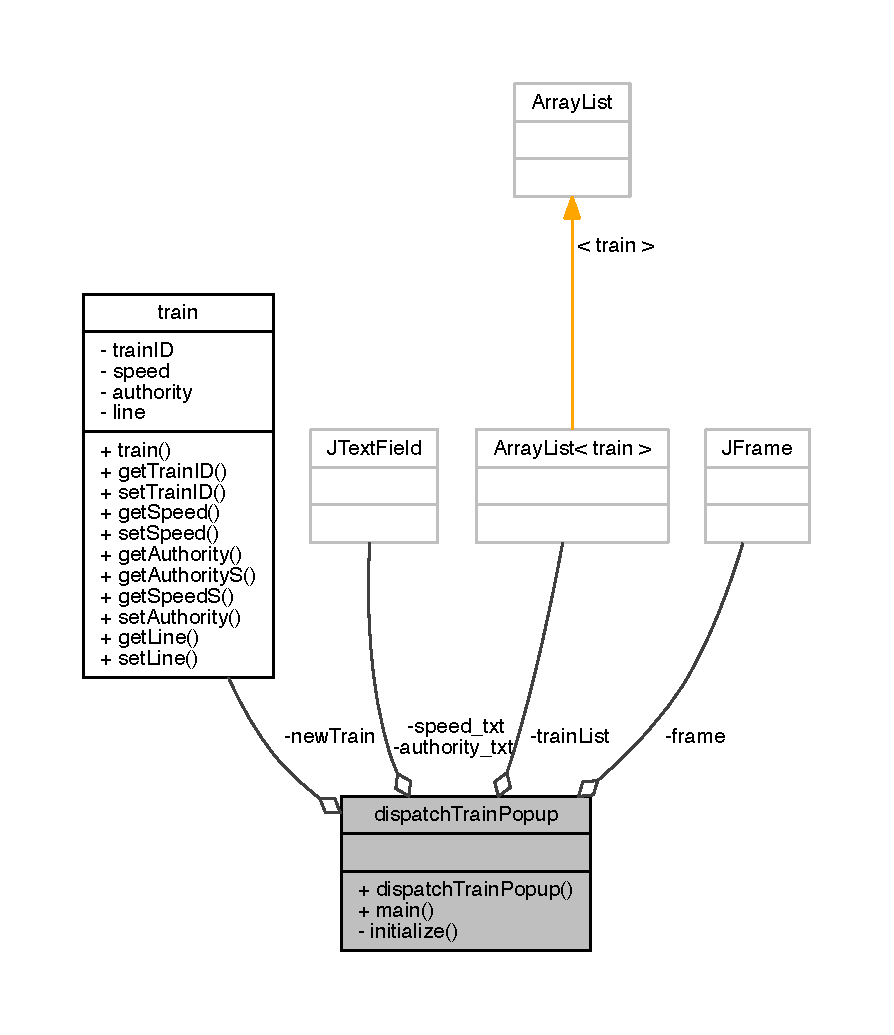
\includegraphics[width=350pt]{classdispatchTrainPopup__coll__graph}
\end{center}
\end{figure}
\subsection*{Public Member Functions}
\begin{DoxyCompactItemize}
\item 
\hyperlink{classdispatchTrainPopup_a993dfedab3089cef6ac33cdee08eb336}{dispatch\+Train\+Popup} (Array\+List$<$ \hyperlink{classtrain}{train} $>$ send\+Trains)
\begin{DoxyCompactList}\small\item\em Create the application. \end{DoxyCompactList}\end{DoxyCompactItemize}
\subsection*{Static Public Member Functions}
\begin{DoxyCompactItemize}
\item 
static void \hyperlink{classdispatchTrainPopup_a339856eed3f163cacde0a351981f1829}{main} (String\mbox{[}$\,$\mbox{]} args)
\begin{DoxyCompactList}\small\item\em Launch the application. \end{DoxyCompactList}\end{DoxyCompactItemize}
\subsection*{Private Member Functions}
\begin{DoxyCompactItemize}
\item 
void \hyperlink{classdispatchTrainPopup_abd0cc81d2cf2f62041d0907ec073f54a}{initialize} (Array\+List$<$ \hyperlink{classtrain}{train} $>$ send\+Trains)
\begin{DoxyCompactList}\small\item\em Initialize the contents of the frame. \end{DoxyCompactList}\end{DoxyCompactItemize}
\subsection*{Private Attributes}
\begin{DoxyCompactItemize}
\item 
J\+Frame \hyperlink{classdispatchTrainPopup_ab5ad8c5fe16cc24bf0777e8c970cedc6}{frame}
\item 
J\+Text\+Field \hyperlink{classdispatchTrainPopup_a16bb03a5f638b24aeed36ef422cfbe7b}{speed\+\_\+txt}
\item 
J\+Text\+Field \hyperlink{classdispatchTrainPopup_af72be221c2943e863a462897b99c3e45}{authority\+\_\+txt}
\item 
\hyperlink{classtrain}{train} \hyperlink{classdispatchTrainPopup_ac2d599056dc80d9fb1f360419db9f13a}{new\+Train}
\end{DoxyCompactItemize}
\subsection*{Static Private Attributes}
\begin{DoxyCompactItemize}
\item 
static Array\+List$<$ \hyperlink{classtrain}{train} $>$ \hyperlink{classdispatchTrainPopup_aeb7e9142a54631b84a4d72dc4b7913dd}{train\+List}
\end{DoxyCompactItemize}


\subsection{Constructor \& Destructor Documentation}
\mbox{\Hypertarget{classdispatchTrainPopup_a993dfedab3089cef6ac33cdee08eb336}\label{classdispatchTrainPopup_a993dfedab3089cef6ac33cdee08eb336}} 
\index{dispatch\+Train\+Popup@{dispatch\+Train\+Popup}!dispatch\+Train\+Popup@{dispatch\+Train\+Popup}}
\index{dispatch\+Train\+Popup@{dispatch\+Train\+Popup}!dispatch\+Train\+Popup@{dispatch\+Train\+Popup}}
\subsubsection{\texorpdfstring{dispatch\+Train\+Popup()}{dispatchTrainPopup()}}
{\footnotesize\ttfamily dispatch\+Train\+Popup.\+dispatch\+Train\+Popup (\begin{DoxyParamCaption}\item[{Array\+List$<$ \hyperlink{classtrain}{train} $>$}]{send\+Trains }\end{DoxyParamCaption})}



Create the application. 



\subsection{Member Function Documentation}
\mbox{\Hypertarget{classdispatchTrainPopup_abd0cc81d2cf2f62041d0907ec073f54a}\label{classdispatchTrainPopup_abd0cc81d2cf2f62041d0907ec073f54a}} 
\index{dispatch\+Train\+Popup@{dispatch\+Train\+Popup}!initialize@{initialize}}
\index{initialize@{initialize}!dispatch\+Train\+Popup@{dispatch\+Train\+Popup}}
\subsubsection{\texorpdfstring{initialize()}{initialize()}}
{\footnotesize\ttfamily void dispatch\+Train\+Popup.\+initialize (\begin{DoxyParamCaption}\item[{Array\+List$<$ \hyperlink{classtrain}{train} $>$}]{send\+Trains }\end{DoxyParamCaption})\hspace{0.3cm}{\ttfamily [private]}}



Initialize the contents of the frame. 

\mbox{\Hypertarget{classdispatchTrainPopup_a339856eed3f163cacde0a351981f1829}\label{classdispatchTrainPopup_a339856eed3f163cacde0a351981f1829}} 
\index{dispatch\+Train\+Popup@{dispatch\+Train\+Popup}!main@{main}}
\index{main@{main}!dispatch\+Train\+Popup@{dispatch\+Train\+Popup}}
\subsubsection{\texorpdfstring{main()}{main()}}
{\footnotesize\ttfamily static void dispatch\+Train\+Popup.\+main (\begin{DoxyParamCaption}\item[{String \mbox{[}$\,$\mbox{]}}]{args }\end{DoxyParamCaption})\hspace{0.3cm}{\ttfamily [static]}}



Launch the application. 



\subsection{Member Data Documentation}
\mbox{\Hypertarget{classdispatchTrainPopup_af72be221c2943e863a462897b99c3e45}\label{classdispatchTrainPopup_af72be221c2943e863a462897b99c3e45}} 
\index{dispatch\+Train\+Popup@{dispatch\+Train\+Popup}!authority\+\_\+txt@{authority\+\_\+txt}}
\index{authority\+\_\+txt@{authority\+\_\+txt}!dispatch\+Train\+Popup@{dispatch\+Train\+Popup}}
\subsubsection{\texorpdfstring{authority\+\_\+txt}{authority\_txt}}
{\footnotesize\ttfamily J\+Text\+Field dispatch\+Train\+Popup.\+authority\+\_\+txt\hspace{0.3cm}{\ttfamily [private]}}

\mbox{\Hypertarget{classdispatchTrainPopup_ab5ad8c5fe16cc24bf0777e8c970cedc6}\label{classdispatchTrainPopup_ab5ad8c5fe16cc24bf0777e8c970cedc6}} 
\index{dispatch\+Train\+Popup@{dispatch\+Train\+Popup}!frame@{frame}}
\index{frame@{frame}!dispatch\+Train\+Popup@{dispatch\+Train\+Popup}}
\subsubsection{\texorpdfstring{frame}{frame}}
{\footnotesize\ttfamily J\+Frame dispatch\+Train\+Popup.\+frame\hspace{0.3cm}{\ttfamily [private]}}

\mbox{\Hypertarget{classdispatchTrainPopup_ac2d599056dc80d9fb1f360419db9f13a}\label{classdispatchTrainPopup_ac2d599056dc80d9fb1f360419db9f13a}} 
\index{dispatch\+Train\+Popup@{dispatch\+Train\+Popup}!new\+Train@{new\+Train}}
\index{new\+Train@{new\+Train}!dispatch\+Train\+Popup@{dispatch\+Train\+Popup}}
\subsubsection{\texorpdfstring{new\+Train}{newTrain}}
{\footnotesize\ttfamily \hyperlink{classtrain}{train} dispatch\+Train\+Popup.\+new\+Train\hspace{0.3cm}{\ttfamily [private]}}

\mbox{\Hypertarget{classdispatchTrainPopup_a16bb03a5f638b24aeed36ef422cfbe7b}\label{classdispatchTrainPopup_a16bb03a5f638b24aeed36ef422cfbe7b}} 
\index{dispatch\+Train\+Popup@{dispatch\+Train\+Popup}!speed\+\_\+txt@{speed\+\_\+txt}}
\index{speed\+\_\+txt@{speed\+\_\+txt}!dispatch\+Train\+Popup@{dispatch\+Train\+Popup}}
\subsubsection{\texorpdfstring{speed\+\_\+txt}{speed\_txt}}
{\footnotesize\ttfamily J\+Text\+Field dispatch\+Train\+Popup.\+speed\+\_\+txt\hspace{0.3cm}{\ttfamily [private]}}

\mbox{\Hypertarget{classdispatchTrainPopup_aeb7e9142a54631b84a4d72dc4b7913dd}\label{classdispatchTrainPopup_aeb7e9142a54631b84a4d72dc4b7913dd}} 
\index{dispatch\+Train\+Popup@{dispatch\+Train\+Popup}!train\+List@{train\+List}}
\index{train\+List@{train\+List}!dispatch\+Train\+Popup@{dispatch\+Train\+Popup}}
\subsubsection{\texorpdfstring{train\+List}{trainList}}
{\footnotesize\ttfamily Array\+List$<$\hyperlink{classtrain}{train}$>$ dispatch\+Train\+Popup.\+train\+List\hspace{0.3cm}{\ttfamily [static]}, {\ttfamily [private]}}



The documentation for this class was generated from the following file\+:\begin{DoxyCompactItemize}
\item 
src/main/java/\+C\+T\+C\+\_\+prototype/src/\hyperlink{dispatchTrainPopup_8java}{dispatch\+Train\+Popup.\+java}\end{DoxyCompactItemize}

\hypertarget{classTrackModelTest_1_1GreenlineTest}{}\section{Track\+Model\+Test.\+Greenline\+Test Class Reference}
\label{classTrackModelTest_1_1GreenlineTest}\index{Track\+Model\+Test.\+Greenline\+Test@{Track\+Model\+Test.\+Greenline\+Test}}


Collaboration diagram for Track\+Model\+Test.\+Greenline\+Test\+:
\nopagebreak
\begin{figure}[H]
\begin{center}
\leavevmode
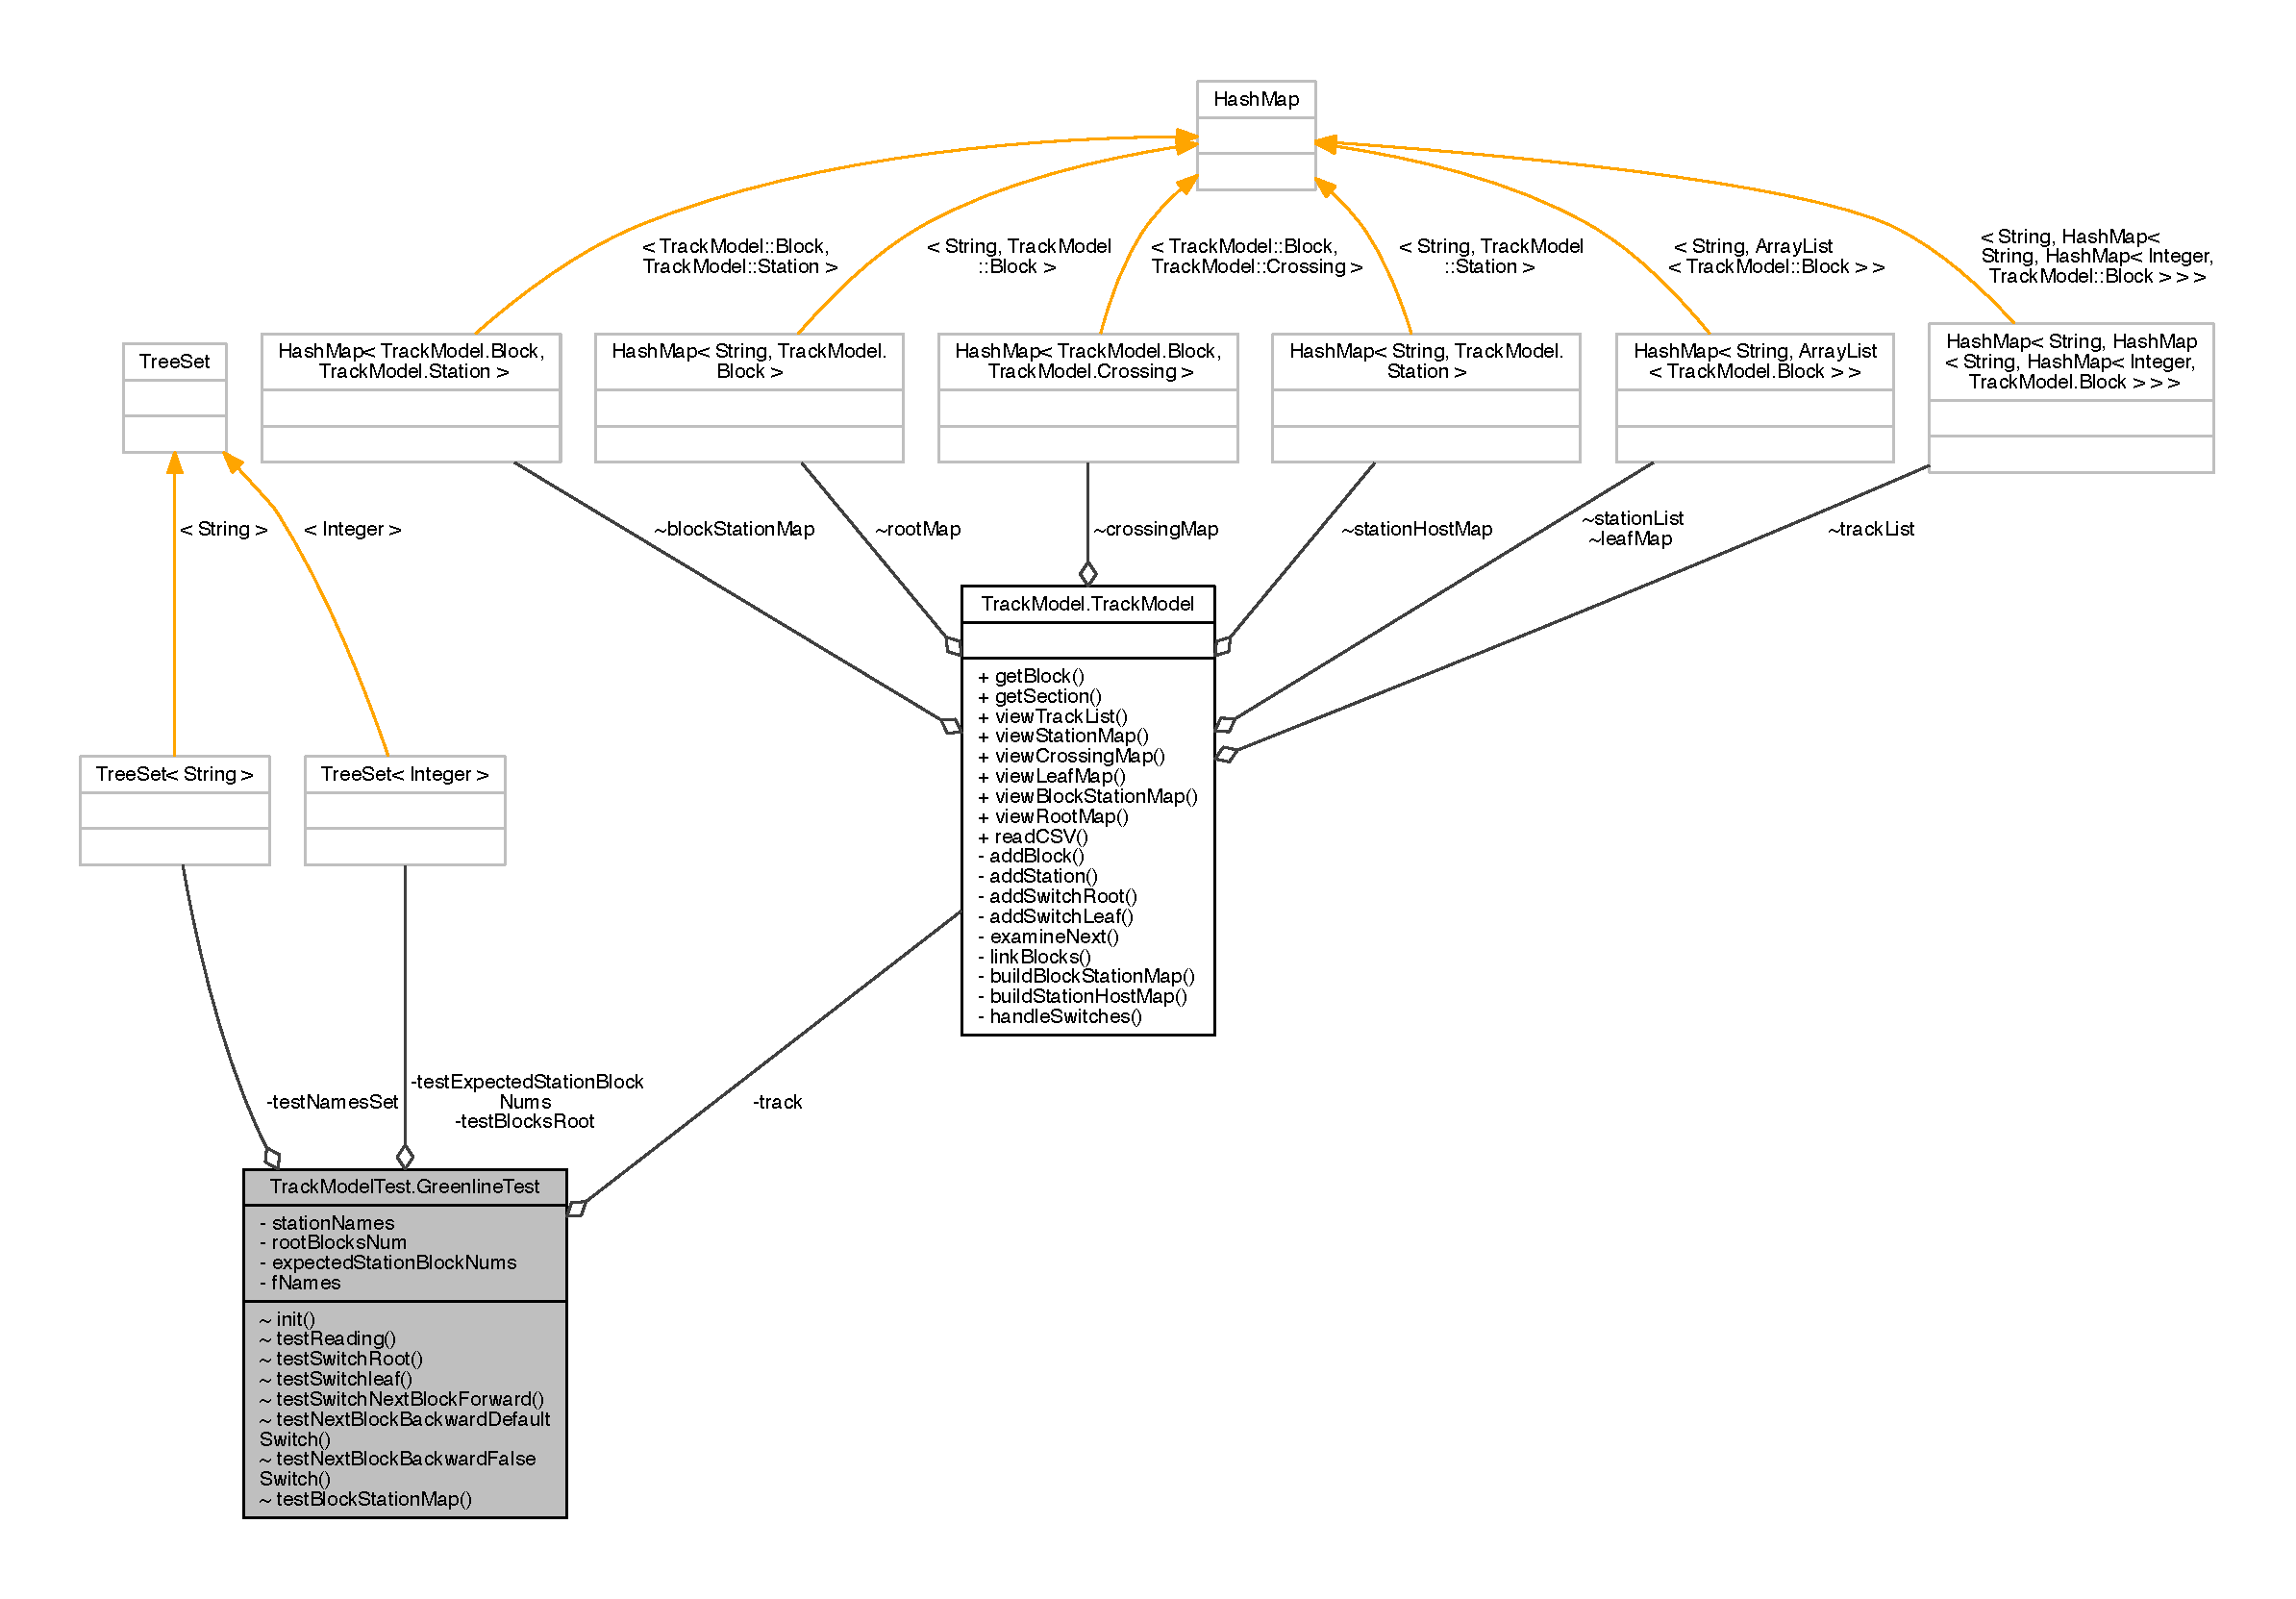
\includegraphics[width=350pt]{classTrackModelTest_1_1GreenlineTest__coll__graph}
\end{center}
\end{figure}
\subsection*{Package Functions}
\begin{DoxyCompactItemize}
\item 
void \hyperlink{classTrackModelTest_1_1GreenlineTest_a3c1cb1eeb41248285ee3e24d71de725c}{init} ()
\item 
void \hyperlink{classTrackModelTest_1_1GreenlineTest_a2f4824d6b276c671fd1204b6a3050931}{test\+Reading} ()
\begin{DoxyCompactList}\small\item\em Test for proper station names reading. \end{DoxyCompactList}\item 
void \hyperlink{classTrackModelTest_1_1GreenlineTest_adbaf11be550589c327cfd7463c1566b2}{test\+Switch\+Root} ()
\begin{DoxyCompactList}\small\item\em Test proper block assignment for switch roots. \end{DoxyCompactList}\item 
void \hyperlink{classTrackModelTest_1_1GreenlineTest_a30c32f186283625347dfd35d4b946f64}{test\+Switchleaf} ()
\begin{DoxyCompactList}\small\item\em Test proper leaf assignments for block on the red line. \end{DoxyCompactList}\item 
void \hyperlink{classTrackModelTest_1_1GreenlineTest_a28f8d0536ddf0225f15cc2e5761bddbd}{test\+Switch\+Next\+Block\+Forward} ()
\begin{DoxyCompactList}\small\item\em Check proper funcitonality of next\+Block\+Forward by switch state on the green line. \end{DoxyCompactList}\item 
void \hyperlink{classTrackModelTest_1_1GreenlineTest_a6d7f0f79f5afa3a6ba6200a41aae0553}{test\+Next\+Block\+Backward\+Default\+Switch} ()
\begin{DoxyCompactList}\small\item\em Check testing of next block backward on the redline. \end{DoxyCompactList}\item 
void \hyperlink{classTrackModelTest_1_1GreenlineTest_abd1ef62857c0df3d5df25ac390edce4b}{test\+Next\+Block\+Backward\+False\+Switch} ()
\begin{DoxyCompactList}\small\item\em Check testing of next block backwards on the redline. \end{DoxyCompactList}\item 
void \hyperlink{classTrackModelTest_1_1GreenlineTest_ad29a8522be040d3f6af724992e63d58d}{test\+Block\+Station\+Map} ()
\begin{DoxyCompactList}\small\item\em Check the functionality of the external block\+Station map for use in the train model and train controller. \end{DoxyCompactList}\end{DoxyCompactItemize}
\subsection*{Static Private Attributes}
\begin{DoxyCompactItemize}
\item 
static String \mbox{[}$\,$\mbox{]} \hyperlink{classTrackModelTest_1_1GreenlineTest_a47a3798d755d618e273ca1a11180db16}{station\+Names}
\item 
static Integer \mbox{[}$\,$\mbox{]} \hyperlink{classTrackModelTest_1_1GreenlineTest_a86d7af0d8ab2f0c855bdca4a06220e1d}{root\+Blocks\+Num} =\{62,13,28,57,77,85\}
\item 
static Integer \mbox{[}$\,$\mbox{]} \hyperlink{classTrackModelTest_1_1GreenlineTest_a70a5b1b7c0ad03d4ee8c021d32fc6585}{expected\+Station\+Block\+Nums} =\{2,9,16,22,31,39,48,57,65,73,77,88,96,105,114,123,132,141,151,152\}
\item 
static Tree\+Set$<$ Integer $>$ \hyperlink{classTrackModelTest_1_1GreenlineTest_aee2fde5125328429838201f535d0aca7}{test\+Blocks\+Root} = new Tree\+Set$<$$>$(Arrays.\+as\+List(\hyperlink{classTrackModelTest_1_1GreenlineTest_a86d7af0d8ab2f0c855bdca4a06220e1d}{root\+Blocks\+Num}))
\item 
static Tree\+Set$<$ String $>$ \hyperlink{classTrackModelTest_1_1GreenlineTest_a3507467040486c396edb29364f5a7bcd}{test\+Names\+Set} = new Tree\+Set$<$$>$(Arrays.\+as\+List(\hyperlink{classTrackModelTest_1_1GreenlineTest_a47a3798d755d618e273ca1a11180db16}{station\+Names}))
\item 
static Tree\+Set$<$ Integer $>$ \hyperlink{classTrackModelTest_1_1GreenlineTest_a96de7e923c81cdf0dd85ece9d95104cc}{test\+Expected\+Station\+Block\+Nums} = new Tree\+Set$<$$>$(Arrays.\+as\+List(\hyperlink{classTrackModelTest_1_1GreenlineTest_a70a5b1b7c0ad03d4ee8c021d32fc6585}{expected\+Station\+Block\+Nums}))
\item 
static \hyperlink{classTrackModel_1_1TrackModel}{Track\+Model} \hyperlink{classTrackModelTest_1_1GreenlineTest_afbfade7894862ab761d49ad840142241}{track}
\item 
static String \mbox{[}$\,$\mbox{]} \hyperlink{classTrackModelTest_1_1GreenlineTest_a02bea164e581cd44c7013e6de9453499}{f\+Names} = \{\char`\"{}src/test/resources/greenline.\+csv\char`\"{}\}
\end{DoxyCompactItemize}


\subsection{Member Function Documentation}
\mbox{\Hypertarget{classTrackModelTest_1_1GreenlineTest_a3c1cb1eeb41248285ee3e24d71de725c}\label{classTrackModelTest_1_1GreenlineTest_a3c1cb1eeb41248285ee3e24d71de725c}} 
\index{Track\+Model\+Test\+::\+Greenline\+Test@{Track\+Model\+Test\+::\+Greenline\+Test}!init@{init}}
\index{init@{init}!Track\+Model\+Test\+::\+Greenline\+Test@{Track\+Model\+Test\+::\+Greenline\+Test}}
\subsubsection{\texorpdfstring{init()}{init()}}
{\footnotesize\ttfamily void Track\+Model\+Test.\+Greenline\+Test.\+init (\begin{DoxyParamCaption}{ }\end{DoxyParamCaption})\hspace{0.3cm}{\ttfamily [package]}}

\mbox{\Hypertarget{classTrackModelTest_1_1GreenlineTest_ad29a8522be040d3f6af724992e63d58d}\label{classTrackModelTest_1_1GreenlineTest_ad29a8522be040d3f6af724992e63d58d}} 
\index{Track\+Model\+Test\+::\+Greenline\+Test@{Track\+Model\+Test\+::\+Greenline\+Test}!test\+Block\+Station\+Map@{test\+Block\+Station\+Map}}
\index{test\+Block\+Station\+Map@{test\+Block\+Station\+Map}!Track\+Model\+Test\+::\+Greenline\+Test@{Track\+Model\+Test\+::\+Greenline\+Test}}
\subsubsection{\texorpdfstring{test\+Block\+Station\+Map()}{testBlockStationMap()}}
{\footnotesize\ttfamily void Track\+Model\+Test.\+Greenline\+Test.\+test\+Block\+Station\+Map (\begin{DoxyParamCaption}{ }\end{DoxyParamCaption})\hspace{0.3cm}{\ttfamily [package]}}



Check the functionality of the external block\+Station map for use in the train model and train controller. 

\mbox{\Hypertarget{classTrackModelTest_1_1GreenlineTest_a6d7f0f79f5afa3a6ba6200a41aae0553}\label{classTrackModelTest_1_1GreenlineTest_a6d7f0f79f5afa3a6ba6200a41aae0553}} 
\index{Track\+Model\+Test\+::\+Greenline\+Test@{Track\+Model\+Test\+::\+Greenline\+Test}!test\+Next\+Block\+Backward\+Default\+Switch@{test\+Next\+Block\+Backward\+Default\+Switch}}
\index{test\+Next\+Block\+Backward\+Default\+Switch@{test\+Next\+Block\+Backward\+Default\+Switch}!Track\+Model\+Test\+::\+Greenline\+Test@{Track\+Model\+Test\+::\+Greenline\+Test}}
\subsubsection{\texorpdfstring{test\+Next\+Block\+Backward\+Default\+Switch()}{testNextBlockBackwardDefaultSwitch()}}
{\footnotesize\ttfamily void Track\+Model\+Test.\+Greenline\+Test.\+test\+Next\+Block\+Backward\+Default\+Switch (\begin{DoxyParamCaption}{ }\end{DoxyParamCaption})\hspace{0.3cm}{\ttfamily [package]}}



Check testing of next block backward on the redline. 

For a \char`\"{}true\char`\"{} (default switch state), the nex\+Block\+Backward should return the root\+Block for the lower indexed block. \mbox{\Hypertarget{classTrackModelTest_1_1GreenlineTest_abd1ef62857c0df3d5df25ac390edce4b}\label{classTrackModelTest_1_1GreenlineTest_abd1ef62857c0df3d5df25ac390edce4b}} 
\index{Track\+Model\+Test\+::\+Greenline\+Test@{Track\+Model\+Test\+::\+Greenline\+Test}!test\+Next\+Block\+Backward\+False\+Switch@{test\+Next\+Block\+Backward\+False\+Switch}}
\index{test\+Next\+Block\+Backward\+False\+Switch@{test\+Next\+Block\+Backward\+False\+Switch}!Track\+Model\+Test\+::\+Greenline\+Test@{Track\+Model\+Test\+::\+Greenline\+Test}}
\subsubsection{\texorpdfstring{test\+Next\+Block\+Backward\+False\+Switch()}{testNextBlockBackwardFalseSwitch()}}
{\footnotesize\ttfamily void Track\+Model\+Test.\+Greenline\+Test.\+test\+Next\+Block\+Backward\+False\+Switch (\begin{DoxyParamCaption}{ }\end{DoxyParamCaption})\hspace{0.3cm}{\ttfamily [package]}}



Check testing of next block backwards on the redline. 

For a \char`\"{}false\char`\"{} (non-\/default switch state), the next\+Block\+Backward should return the root\+Block for the higher indexed block. \mbox{\Hypertarget{classTrackModelTest_1_1GreenlineTest_a2f4824d6b276c671fd1204b6a3050931}\label{classTrackModelTest_1_1GreenlineTest_a2f4824d6b276c671fd1204b6a3050931}} 
\index{Track\+Model\+Test\+::\+Greenline\+Test@{Track\+Model\+Test\+::\+Greenline\+Test}!test\+Reading@{test\+Reading}}
\index{test\+Reading@{test\+Reading}!Track\+Model\+Test\+::\+Greenline\+Test@{Track\+Model\+Test\+::\+Greenline\+Test}}
\subsubsection{\texorpdfstring{test\+Reading()}{testReading()}}
{\footnotesize\ttfamily void Track\+Model\+Test.\+Greenline\+Test.\+test\+Reading (\begin{DoxyParamCaption}{ }\end{DoxyParamCaption})\hspace{0.3cm}{\ttfamily [package]}}



Test for proper station names reading. 

\mbox{\Hypertarget{classTrackModelTest_1_1GreenlineTest_a30c32f186283625347dfd35d4b946f64}\label{classTrackModelTest_1_1GreenlineTest_a30c32f186283625347dfd35d4b946f64}} 
\index{Track\+Model\+Test\+::\+Greenline\+Test@{Track\+Model\+Test\+::\+Greenline\+Test}!test\+Switchleaf@{test\+Switchleaf}}
\index{test\+Switchleaf@{test\+Switchleaf}!Track\+Model\+Test\+::\+Greenline\+Test@{Track\+Model\+Test\+::\+Greenline\+Test}}
\subsubsection{\texorpdfstring{test\+Switchleaf()}{testSwitchleaf()}}
{\footnotesize\ttfamily void Track\+Model\+Test.\+Greenline\+Test.\+test\+Switchleaf (\begin{DoxyParamCaption}{ }\end{DoxyParamCaption})\hspace{0.3cm}{\ttfamily [package]}}



Test proper leaf assignments for block on the red line. 

\mbox{\Hypertarget{classTrackModelTest_1_1GreenlineTest_a28f8d0536ddf0225f15cc2e5761bddbd}\label{classTrackModelTest_1_1GreenlineTest_a28f8d0536ddf0225f15cc2e5761bddbd}} 
\index{Track\+Model\+Test\+::\+Greenline\+Test@{Track\+Model\+Test\+::\+Greenline\+Test}!test\+Switch\+Next\+Block\+Forward@{test\+Switch\+Next\+Block\+Forward}}
\index{test\+Switch\+Next\+Block\+Forward@{test\+Switch\+Next\+Block\+Forward}!Track\+Model\+Test\+::\+Greenline\+Test@{Track\+Model\+Test\+::\+Greenline\+Test}}
\subsubsection{\texorpdfstring{test\+Switch\+Next\+Block\+Forward()}{testSwitchNextBlockForward()}}
{\footnotesize\ttfamily void Track\+Model\+Test.\+Greenline\+Test.\+test\+Switch\+Next\+Block\+Forward (\begin{DoxyParamCaption}{ }\end{DoxyParamCaption})\hspace{0.3cm}{\ttfamily [package]}}



Check proper funcitonality of next\+Block\+Forward by switch state on the green line. 

\mbox{\Hypertarget{classTrackModelTest_1_1GreenlineTest_adbaf11be550589c327cfd7463c1566b2}\label{classTrackModelTest_1_1GreenlineTest_adbaf11be550589c327cfd7463c1566b2}} 
\index{Track\+Model\+Test\+::\+Greenline\+Test@{Track\+Model\+Test\+::\+Greenline\+Test}!test\+Switch\+Root@{test\+Switch\+Root}}
\index{test\+Switch\+Root@{test\+Switch\+Root}!Track\+Model\+Test\+::\+Greenline\+Test@{Track\+Model\+Test\+::\+Greenline\+Test}}
\subsubsection{\texorpdfstring{test\+Switch\+Root()}{testSwitchRoot()}}
{\footnotesize\ttfamily void Track\+Model\+Test.\+Greenline\+Test.\+test\+Switch\+Root (\begin{DoxyParamCaption}{ }\end{DoxyParamCaption})\hspace{0.3cm}{\ttfamily [package]}}



Test proper block assignment for switch roots. 



\subsection{Member Data Documentation}
\mbox{\Hypertarget{classTrackModelTest_1_1GreenlineTest_a70a5b1b7c0ad03d4ee8c021d32fc6585}\label{classTrackModelTest_1_1GreenlineTest_a70a5b1b7c0ad03d4ee8c021d32fc6585}} 
\index{Track\+Model\+Test\+::\+Greenline\+Test@{Track\+Model\+Test\+::\+Greenline\+Test}!expected\+Station\+Block\+Nums@{expected\+Station\+Block\+Nums}}
\index{expected\+Station\+Block\+Nums@{expected\+Station\+Block\+Nums}!Track\+Model\+Test\+::\+Greenline\+Test@{Track\+Model\+Test\+::\+Greenline\+Test}}
\subsubsection{\texorpdfstring{expected\+Station\+Block\+Nums}{expectedStationBlockNums}}
{\footnotesize\ttfamily Integer \mbox{[}$\,$\mbox{]} Track\+Model\+Test.\+Greenline\+Test.\+expected\+Station\+Block\+Nums =\{2,9,16,22,31,39,48,57,65,73,77,88,96,105,114,123,132,141,151,152\}\hspace{0.3cm}{\ttfamily [static]}, {\ttfamily [private]}}

\mbox{\Hypertarget{classTrackModelTest_1_1GreenlineTest_a02bea164e581cd44c7013e6de9453499}\label{classTrackModelTest_1_1GreenlineTest_a02bea164e581cd44c7013e6de9453499}} 
\index{Track\+Model\+Test\+::\+Greenline\+Test@{Track\+Model\+Test\+::\+Greenline\+Test}!f\+Names@{f\+Names}}
\index{f\+Names@{f\+Names}!Track\+Model\+Test\+::\+Greenline\+Test@{Track\+Model\+Test\+::\+Greenline\+Test}}
\subsubsection{\texorpdfstring{f\+Names}{fNames}}
{\footnotesize\ttfamily String \mbox{[}$\,$\mbox{]} Track\+Model\+Test.\+Greenline\+Test.\+f\+Names = \{\char`\"{}src/test/resources/greenline.\+csv\char`\"{}\}\hspace{0.3cm}{\ttfamily [static]}, {\ttfamily [private]}}

\mbox{\Hypertarget{classTrackModelTest_1_1GreenlineTest_a86d7af0d8ab2f0c855bdca4a06220e1d}\label{classTrackModelTest_1_1GreenlineTest_a86d7af0d8ab2f0c855bdca4a06220e1d}} 
\index{Track\+Model\+Test\+::\+Greenline\+Test@{Track\+Model\+Test\+::\+Greenline\+Test}!root\+Blocks\+Num@{root\+Blocks\+Num}}
\index{root\+Blocks\+Num@{root\+Blocks\+Num}!Track\+Model\+Test\+::\+Greenline\+Test@{Track\+Model\+Test\+::\+Greenline\+Test}}
\subsubsection{\texorpdfstring{root\+Blocks\+Num}{rootBlocksNum}}
{\footnotesize\ttfamily Integer \mbox{[}$\,$\mbox{]} Track\+Model\+Test.\+Greenline\+Test.\+root\+Blocks\+Num =\{62,13,28,57,77,85\}\hspace{0.3cm}{\ttfamily [static]}, {\ttfamily [private]}}

\mbox{\Hypertarget{classTrackModelTest_1_1GreenlineTest_a47a3798d755d618e273ca1a11180db16}\label{classTrackModelTest_1_1GreenlineTest_a47a3798d755d618e273ca1a11180db16}} 
\index{Track\+Model\+Test\+::\+Greenline\+Test@{Track\+Model\+Test\+::\+Greenline\+Test}!station\+Names@{station\+Names}}
\index{station\+Names@{station\+Names}!Track\+Model\+Test\+::\+Greenline\+Test@{Track\+Model\+Test\+::\+Greenline\+Test}}
\subsubsection{\texorpdfstring{station\+Names}{stationNames}}
{\footnotesize\ttfamily String \mbox{[}$\,$\mbox{]} Track\+Model\+Test.\+Greenline\+Test.\+station\+Names\hspace{0.3cm}{\ttfamily [static]}, {\ttfamily [private]}}

{\bfseries Initial value\+:}
\begin{DoxyCode}
=\{\textcolor{stringliteral}{"OVERBROOK"}, \textcolor{stringliteral}{"UNIVERSITY OF PITTSBURGH"}, \textcolor{stringliteral}{"CENTRAL"}, \textcolor{stringliteral}{"POPLAR"}, \textcolor{stringliteral}{"CASTLE SHANNON"}, 
                                        \textcolor{stringliteral}{"DORMONT"}, \textcolor{stringliteral}{"SOUTH BANK"}, \textcolor{stringliteral}{"WHITED"}, \textcolor{stringliteral}{"MT LEBANON"}, \textcolor{stringliteral}{"INGLEWOOD"}, \textcolor{stringliteral}{"
      PIONEER"}, \textcolor{stringliteral}{"EDGEBROOK"}, 
                                        \textcolor{stringliteral}{"GLENBURY"},\textcolor{stringliteral}{"YARD"}\}
\end{DoxyCode}
\mbox{\Hypertarget{classTrackModelTest_1_1GreenlineTest_aee2fde5125328429838201f535d0aca7}\label{classTrackModelTest_1_1GreenlineTest_aee2fde5125328429838201f535d0aca7}} 
\index{Track\+Model\+Test\+::\+Greenline\+Test@{Track\+Model\+Test\+::\+Greenline\+Test}!test\+Blocks\+Root@{test\+Blocks\+Root}}
\index{test\+Blocks\+Root@{test\+Blocks\+Root}!Track\+Model\+Test\+::\+Greenline\+Test@{Track\+Model\+Test\+::\+Greenline\+Test}}
\subsubsection{\texorpdfstring{test\+Blocks\+Root}{testBlocksRoot}}
{\footnotesize\ttfamily Tree\+Set$<$Integer$>$ Track\+Model\+Test.\+Greenline\+Test.\+test\+Blocks\+Root = new Tree\+Set$<$$>$(Arrays.\+as\+List(\hyperlink{classTrackModelTest_1_1GreenlineTest_a86d7af0d8ab2f0c855bdca4a06220e1d}{root\+Blocks\+Num}))\hspace{0.3cm}{\ttfamily [static]}, {\ttfamily [private]}}

\mbox{\Hypertarget{classTrackModelTest_1_1GreenlineTest_a96de7e923c81cdf0dd85ece9d95104cc}\label{classTrackModelTest_1_1GreenlineTest_a96de7e923c81cdf0dd85ece9d95104cc}} 
\index{Track\+Model\+Test\+::\+Greenline\+Test@{Track\+Model\+Test\+::\+Greenline\+Test}!test\+Expected\+Station\+Block\+Nums@{test\+Expected\+Station\+Block\+Nums}}
\index{test\+Expected\+Station\+Block\+Nums@{test\+Expected\+Station\+Block\+Nums}!Track\+Model\+Test\+::\+Greenline\+Test@{Track\+Model\+Test\+::\+Greenline\+Test}}
\subsubsection{\texorpdfstring{test\+Expected\+Station\+Block\+Nums}{testExpectedStationBlockNums}}
{\footnotesize\ttfamily Tree\+Set$<$Integer$>$ Track\+Model\+Test.\+Greenline\+Test.\+test\+Expected\+Station\+Block\+Nums = new Tree\+Set$<$$>$(Arrays.\+as\+List(\hyperlink{classTrackModelTest_1_1GreenlineTest_a70a5b1b7c0ad03d4ee8c021d32fc6585}{expected\+Station\+Block\+Nums}))\hspace{0.3cm}{\ttfamily [static]}, {\ttfamily [private]}}

\mbox{\Hypertarget{classTrackModelTest_1_1GreenlineTest_a3507467040486c396edb29364f5a7bcd}\label{classTrackModelTest_1_1GreenlineTest_a3507467040486c396edb29364f5a7bcd}} 
\index{Track\+Model\+Test\+::\+Greenline\+Test@{Track\+Model\+Test\+::\+Greenline\+Test}!test\+Names\+Set@{test\+Names\+Set}}
\index{test\+Names\+Set@{test\+Names\+Set}!Track\+Model\+Test\+::\+Greenline\+Test@{Track\+Model\+Test\+::\+Greenline\+Test}}
\subsubsection{\texorpdfstring{test\+Names\+Set}{testNamesSet}}
{\footnotesize\ttfamily Tree\+Set$<$String$>$ Track\+Model\+Test.\+Greenline\+Test.\+test\+Names\+Set = new Tree\+Set$<$$>$(Arrays.\+as\+List(\hyperlink{classTrackModelTest_1_1GreenlineTest_a47a3798d755d618e273ca1a11180db16}{station\+Names}))\hspace{0.3cm}{\ttfamily [static]}, {\ttfamily [private]}}

\mbox{\Hypertarget{classTrackModelTest_1_1GreenlineTest_afbfade7894862ab761d49ad840142241}\label{classTrackModelTest_1_1GreenlineTest_afbfade7894862ab761d49ad840142241}} 
\index{Track\+Model\+Test\+::\+Greenline\+Test@{Track\+Model\+Test\+::\+Greenline\+Test}!track@{track}}
\index{track@{track}!Track\+Model\+Test\+::\+Greenline\+Test@{Track\+Model\+Test\+::\+Greenline\+Test}}
\subsubsection{\texorpdfstring{track}{track}}
{\footnotesize\ttfamily \hyperlink{classTrackModel_1_1TrackModel}{Track\+Model} Track\+Model\+Test.\+Greenline\+Test.\+track\hspace{0.3cm}{\ttfamily [static]}, {\ttfamily [private]}}



The documentation for this class was generated from the following file\+:\begin{DoxyCompactItemize}
\item 
src/test/java/\+Track\+Model\+Test/\hyperlink{GreenlineTest_8java}{Greenline\+Test.\+java}\end{DoxyCompactItemize}

\hypertarget{classlaunch}{}\section{launch Class Reference}
\label{classlaunch}\index{launch@{launch}}


Collaboration diagram for launch\+:
\nopagebreak
\begin{figure}[H]
\begin{center}
\leavevmode
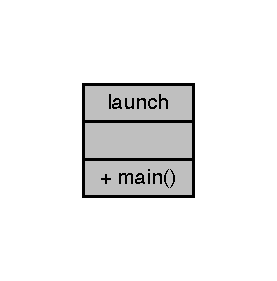
\includegraphics[width=133pt]{classlaunch__coll__graph}
\end{center}
\end{figure}
\subsection*{Static Public Member Functions}
\begin{DoxyCompactItemize}
\item 
static void \hyperlink{classlaunch_a19aea6ad098436eb0709e850e4c5b41d}{main} (String\mbox{[}$\,$\mbox{]} args)
\end{DoxyCompactItemize}


\subsection{Member Function Documentation}
\mbox{\Hypertarget{classlaunch_a19aea6ad098436eb0709e850e4c5b41d}\label{classlaunch_a19aea6ad098436eb0709e850e4c5b41d}} 
\index{launch@{launch}!main@{main}}
\index{main@{main}!launch@{launch}}
\subsubsection{\texorpdfstring{main()}{main()}}
{\footnotesize\ttfamily static void launch.\+main (\begin{DoxyParamCaption}\item[{String \mbox{[}$\,$\mbox{]}}]{args }\end{DoxyParamCaption})\hspace{0.3cm}{\ttfamily [static]}}



The documentation for this class was generated from the following file\+:\begin{DoxyCompactItemize}
\item 
src/main/java/\+C\+T\+C\+\_\+prototype/src/\hyperlink{launch_8java}{launch.\+java}\end{DoxyCompactItemize}

\hypertarget{classtrainModel_1_1Launch}{}\section{train\+Model.\+Launch Class Reference}
\label{classtrainModel_1_1Launch}\index{train\+Model.\+Launch@{train\+Model.\+Launch}}


Collaboration diagram for train\+Model.\+Launch\+:
\nopagebreak
\begin{figure}[H]
\begin{center}
\leavevmode
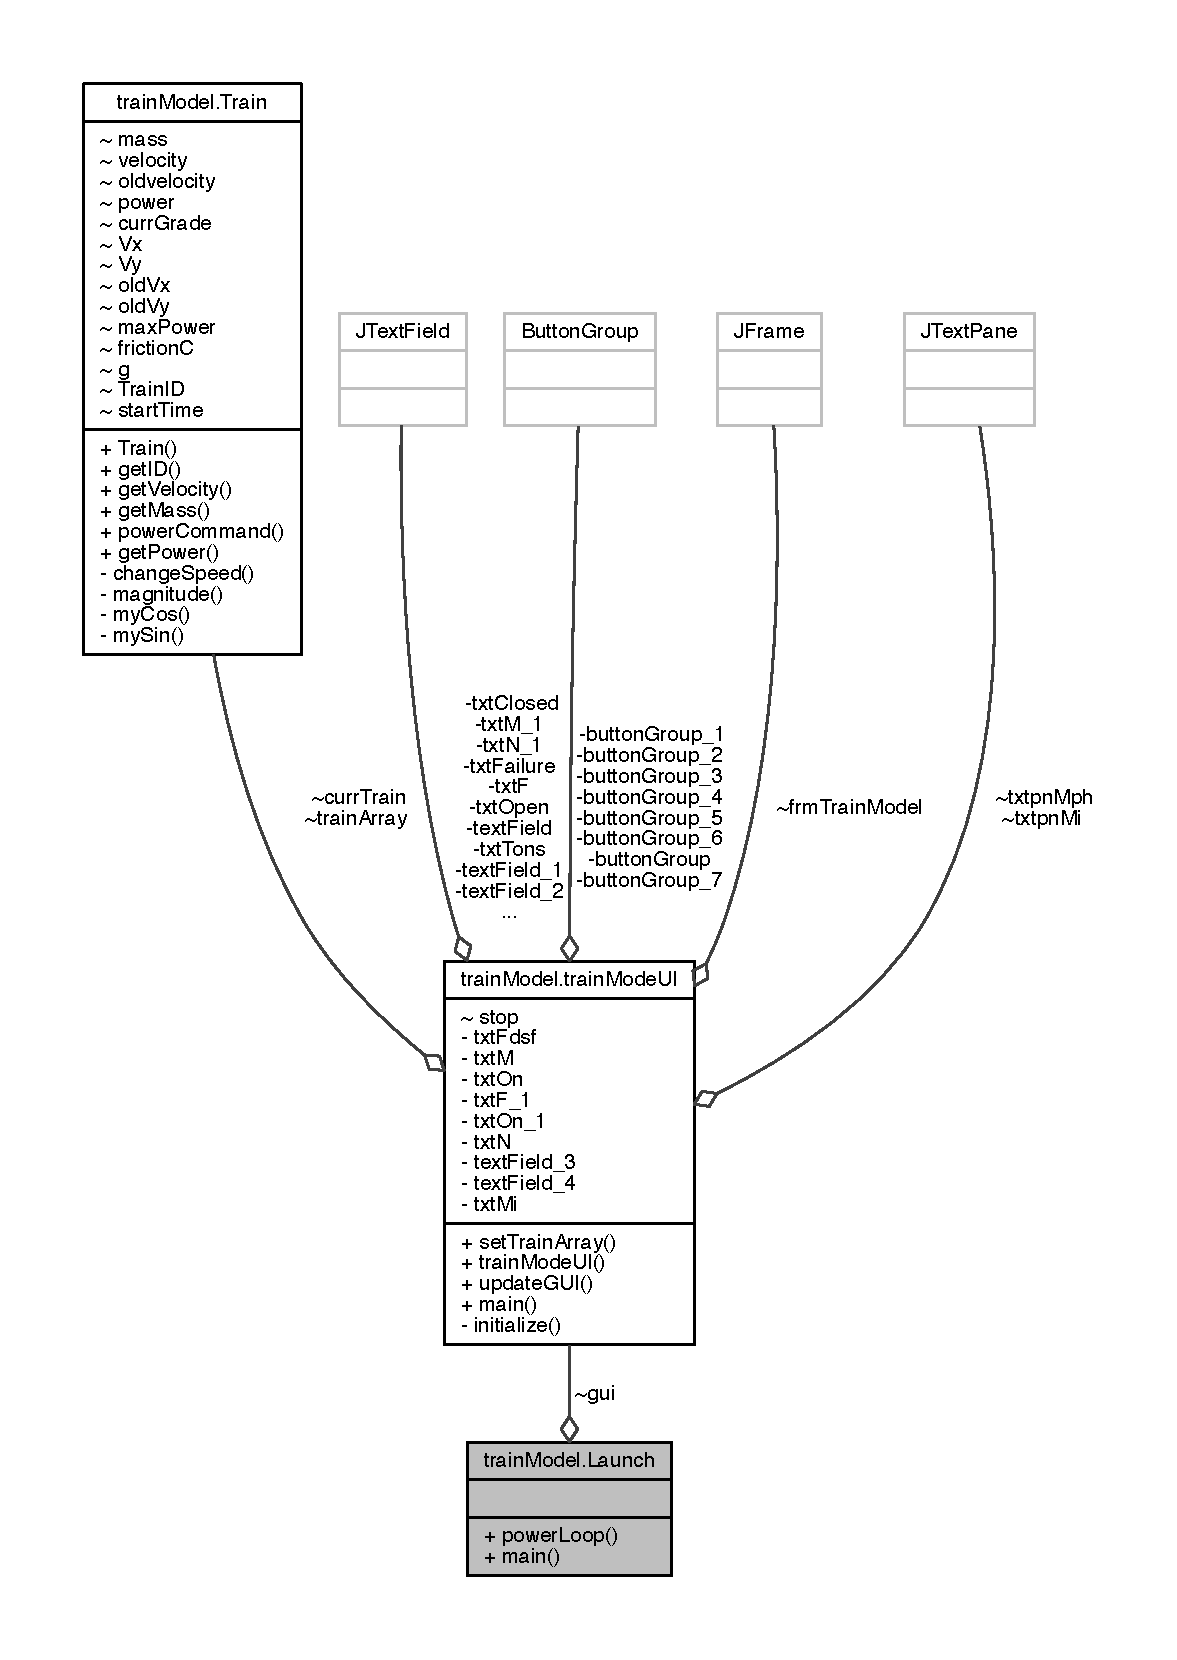
\includegraphics[width=350pt]{classtrainModel_1_1Launch__coll__graph}
\end{center}
\end{figure}
\subsection*{Public Member Functions}
\begin{DoxyCompactItemize}
\item 
void \hyperlink{classtrainModel_1_1Launch_aeb9937905b93f52cdfef74d098988e8d}{power\+Loop} (Double pow, \hyperlink{classtrainModel_1_1Train}{Train} currT)
\end{DoxyCompactItemize}
\subsection*{Static Public Member Functions}
\begin{DoxyCompactItemize}
\item 
static void \hyperlink{classtrainModel_1_1Launch_a94e43f9ec39a2fd0fec5144eff076f34}{main} (String \mbox{[}$\,$\mbox{]} args)
\end{DoxyCompactItemize}
\subsection*{Static Package Attributes}
\begin{DoxyCompactItemize}
\item 
static \hyperlink{classtrainModel_1_1trainModeUI}{train\+Mode\+UI} \hyperlink{classtrainModel_1_1Launch_a54ad9d8c3da59d4e2aaca7bb7e73df6f}{gui} = new \hyperlink{classtrainModel_1_1trainModeUI}{train\+Mode\+UI}()
\end{DoxyCompactItemize}


\subsection{Member Function Documentation}
\mbox{\Hypertarget{classtrainModel_1_1Launch_a94e43f9ec39a2fd0fec5144eff076f34}\label{classtrainModel_1_1Launch_a94e43f9ec39a2fd0fec5144eff076f34}} 
\index{train\+Model\+::\+Launch@{train\+Model\+::\+Launch}!main@{main}}
\index{main@{main}!train\+Model\+::\+Launch@{train\+Model\+::\+Launch}}
\subsubsection{\texorpdfstring{main()}{main()}}
{\footnotesize\ttfamily static void train\+Model.\+Launch.\+main (\begin{DoxyParamCaption}\item[{String \mbox{[}$\,$\mbox{]}}]{args }\end{DoxyParamCaption})\hspace{0.3cm}{\ttfamily [static]}}

\mbox{\Hypertarget{classtrainModel_1_1Launch_aeb9937905b93f52cdfef74d098988e8d}\label{classtrainModel_1_1Launch_aeb9937905b93f52cdfef74d098988e8d}} 
\index{train\+Model\+::\+Launch@{train\+Model\+::\+Launch}!power\+Loop@{power\+Loop}}
\index{power\+Loop@{power\+Loop}!train\+Model\+::\+Launch@{train\+Model\+::\+Launch}}
\subsubsection{\texorpdfstring{power\+Loop()}{powerLoop()}}
{\footnotesize\ttfamily void train\+Model.\+Launch.\+power\+Loop (\begin{DoxyParamCaption}\item[{Double}]{pow,  }\item[{\hyperlink{classtrainModel_1_1Train}{Train}}]{currT }\end{DoxyParamCaption})}



\subsection{Member Data Documentation}
\mbox{\Hypertarget{classtrainModel_1_1Launch_a54ad9d8c3da59d4e2aaca7bb7e73df6f}\label{classtrainModel_1_1Launch_a54ad9d8c3da59d4e2aaca7bb7e73df6f}} 
\index{train\+Model\+::\+Launch@{train\+Model\+::\+Launch}!gui@{gui}}
\index{gui@{gui}!train\+Model\+::\+Launch@{train\+Model\+::\+Launch}}
\subsubsection{\texorpdfstring{gui}{gui}}
{\footnotesize\ttfamily \hyperlink{classtrainModel_1_1trainModeUI}{train\+Mode\+UI} train\+Model.\+Launch.\+gui = new \hyperlink{classtrainModel_1_1trainModeUI}{train\+Mode\+UI}()\hspace{0.3cm}{\ttfamily [static]}, {\ttfamily [package]}}



The documentation for this class was generated from the following file\+:\begin{DoxyCompactItemize}
\item 
src/main/java/train\+Model/\hyperlink{Launch_8java}{Launch.\+java}\end{DoxyCompactItemize}

\hypertarget{classLauncher}{}\section{Launcher Class Reference}
\label{classLauncher}\index{Launcher@{Launcher}}


Collaboration diagram for Launcher\+:
\nopagebreak
\begin{figure}[H]
\begin{center}
\leavevmode
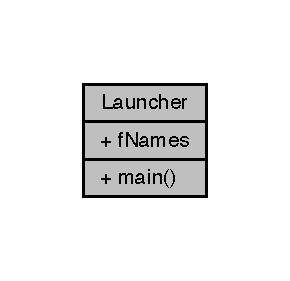
\includegraphics[width=139pt]{classLauncher__coll__graph}
\end{center}
\end{figure}
\subsection*{Static Public Member Functions}
\begin{DoxyCompactItemize}
\item 
static void \hyperlink{classLauncher_aa9770583b7ae34ee983017a915933f9f}{main} (String\mbox{[}$\,$\mbox{]} args)
\end{DoxyCompactItemize}
\subsection*{Static Public Attributes}
\begin{DoxyCompactItemize}
\item 
static final String \mbox{[}$\,$\mbox{]} \hyperlink{classLauncher_a87e12281d7d005f72571c3bbf569dbf2}{f\+Names} = \{\char`\"{}resources/redline.\+csv\char`\"{}\}
\end{DoxyCompactItemize}


\subsection{Member Function Documentation}
\mbox{\Hypertarget{classLauncher_aa9770583b7ae34ee983017a915933f9f}\label{classLauncher_aa9770583b7ae34ee983017a915933f9f}} 
\index{Launcher@{Launcher}!main@{main}}
\index{main@{main}!Launcher@{Launcher}}
\subsubsection{\texorpdfstring{main()}{main()}}
{\footnotesize\ttfamily static void Launcher.\+main (\begin{DoxyParamCaption}\item[{String \mbox{[}$\,$\mbox{]}}]{args }\end{DoxyParamCaption})\hspace{0.3cm}{\ttfamily [static]}}



\subsection{Member Data Documentation}
\mbox{\Hypertarget{classLauncher_a87e12281d7d005f72571c3bbf569dbf2}\label{classLauncher_a87e12281d7d005f72571c3bbf569dbf2}} 
\index{Launcher@{Launcher}!f\+Names@{f\+Names}}
\index{f\+Names@{f\+Names}!Launcher@{Launcher}}
\subsubsection{\texorpdfstring{f\+Names}{fNames}}
{\footnotesize\ttfamily final String \mbox{[}$\,$\mbox{]} Launcher.\+f\+Names = \{\char`\"{}resources/redline.\+csv\char`\"{}\}\hspace{0.3cm}{\ttfamily [static]}}



The documentation for this class was generated from the following file\+:\begin{DoxyCompactItemize}
\item 
src/main/java/\hyperlink{Launcher_8java}{Launcher.\+java}\end{DoxyCompactItemize}

\hypertarget{classWaysideController_1_1PLC}{}\section{Wayside\+Controller.\+P\+LC Class Reference}
\label{classWaysideController_1_1PLC}\index{Wayside\+Controller.\+P\+LC@{Wayside\+Controller.\+P\+LC}}


Collaboration diagram for Wayside\+Controller.\+P\+LC\+:
\nopagebreak
\begin{figure}[H]
\begin{center}
\leavevmode
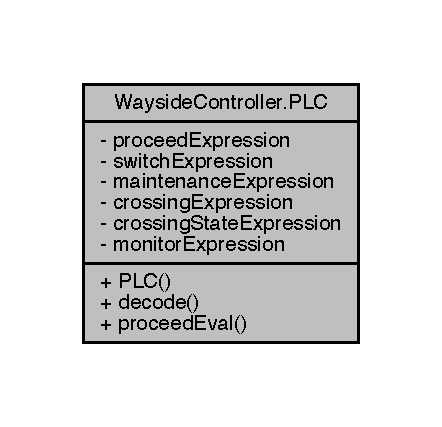
\includegraphics[width=212pt]{classWaysideController_1_1PLC__coll__graph}
\end{center}
\end{figure}
\subsection*{Public Member Functions}
\begin{DoxyCompactItemize}
\item 
\hyperlink{classWaysideController_1_1PLC_af4c4636b44883be330c95dadb07ce0b9}{P\+LC} (String pE, String sE, String maE, String cE, String csE, String moE)
\item 
void \hyperlink{classWaysideController_1_1PLC_a22c9f62b45d4af0d977188967cb40134}{decode} ()
\item 
boolean \hyperlink{classWaysideController_1_1PLC_aa744955096a2d7156c6ad8a798c6db08}{proceed\+Eval} (\hyperlink{classTrackModel_1_1Block}{Block} b)  throws Script\+Exception
\end{DoxyCompactItemize}
\subsection*{Private Attributes}
\begin{DoxyCompactItemize}
\item 
String \hyperlink{classWaysideController_1_1PLC_affffe6e548e3e627c44fda340ff6b65b}{proceed\+Expression}
\item 
String \hyperlink{classWaysideController_1_1PLC_ab6616556bdf225a697db35a4d330024e}{switch\+Expression}
\item 
String \hyperlink{classWaysideController_1_1PLC_aaf3416f0f6eb620ef9dc9745a2a27617}{maintenance\+Expression}
\item 
String \hyperlink{classWaysideController_1_1PLC_acafd6381b97c21f60f1267e7b98f70f1}{crossing\+Expression}
\item 
String \hyperlink{classWaysideController_1_1PLC_a1c05e7c7479c250f83500a2fde0a03d4}{crossing\+State\+Expression}
\item 
String \hyperlink{classWaysideController_1_1PLC_a524d834de5024e021c8e21bbdb27af99}{monitor\+Expression}
\end{DoxyCompactItemize}


\subsection{Constructor \& Destructor Documentation}
\mbox{\Hypertarget{classWaysideController_1_1PLC_af4c4636b44883be330c95dadb07ce0b9}\label{classWaysideController_1_1PLC_af4c4636b44883be330c95dadb07ce0b9}} 
\index{Wayside\+Controller\+::\+P\+LC@{Wayside\+Controller\+::\+P\+LC}!P\+LC@{P\+LC}}
\index{P\+LC@{P\+LC}!Wayside\+Controller\+::\+P\+LC@{Wayside\+Controller\+::\+P\+LC}}
\subsubsection{\texorpdfstring{P\+L\+C()}{PLC()}}
{\footnotesize\ttfamily Wayside\+Controller.\+P\+L\+C.\+P\+LC (\begin{DoxyParamCaption}\item[{String}]{pE,  }\item[{String}]{sE,  }\item[{String}]{maE,  }\item[{String}]{cE,  }\item[{String}]{csE,  }\item[{String}]{moE }\end{DoxyParamCaption})}



\subsection{Member Function Documentation}
\mbox{\Hypertarget{classWaysideController_1_1PLC_a22c9f62b45d4af0d977188967cb40134}\label{classWaysideController_1_1PLC_a22c9f62b45d4af0d977188967cb40134}} 
\index{Wayside\+Controller\+::\+P\+LC@{Wayside\+Controller\+::\+P\+LC}!decode@{decode}}
\index{decode@{decode}!Wayside\+Controller\+::\+P\+LC@{Wayside\+Controller\+::\+P\+LC}}
\subsubsection{\texorpdfstring{decode()}{decode()}}
{\footnotesize\ttfamily void Wayside\+Controller.\+P\+L\+C.\+decode (\begin{DoxyParamCaption}{ }\end{DoxyParamCaption})}

\mbox{\Hypertarget{classWaysideController_1_1PLC_aa744955096a2d7156c6ad8a798c6db08}\label{classWaysideController_1_1PLC_aa744955096a2d7156c6ad8a798c6db08}} 
\index{Wayside\+Controller\+::\+P\+LC@{Wayside\+Controller\+::\+P\+LC}!proceed\+Eval@{proceed\+Eval}}
\index{proceed\+Eval@{proceed\+Eval}!Wayside\+Controller\+::\+P\+LC@{Wayside\+Controller\+::\+P\+LC}}
\subsubsection{\texorpdfstring{proceed\+Eval()}{proceedEval()}}
{\footnotesize\ttfamily boolean Wayside\+Controller.\+P\+L\+C.\+proceed\+Eval (\begin{DoxyParamCaption}\item[{\hyperlink{classTrackModel_1_1Block}{Block}}]{b }\end{DoxyParamCaption}) throws Script\+Exception}



\subsection{Member Data Documentation}
\mbox{\Hypertarget{classWaysideController_1_1PLC_acafd6381b97c21f60f1267e7b98f70f1}\label{classWaysideController_1_1PLC_acafd6381b97c21f60f1267e7b98f70f1}} 
\index{Wayside\+Controller\+::\+P\+LC@{Wayside\+Controller\+::\+P\+LC}!crossing\+Expression@{crossing\+Expression}}
\index{crossing\+Expression@{crossing\+Expression}!Wayside\+Controller\+::\+P\+LC@{Wayside\+Controller\+::\+P\+LC}}
\subsubsection{\texorpdfstring{crossing\+Expression}{crossingExpression}}
{\footnotesize\ttfamily String Wayside\+Controller.\+P\+L\+C.\+crossing\+Expression\hspace{0.3cm}{\ttfamily [private]}}

\mbox{\Hypertarget{classWaysideController_1_1PLC_a1c05e7c7479c250f83500a2fde0a03d4}\label{classWaysideController_1_1PLC_a1c05e7c7479c250f83500a2fde0a03d4}} 
\index{Wayside\+Controller\+::\+P\+LC@{Wayside\+Controller\+::\+P\+LC}!crossing\+State\+Expression@{crossing\+State\+Expression}}
\index{crossing\+State\+Expression@{crossing\+State\+Expression}!Wayside\+Controller\+::\+P\+LC@{Wayside\+Controller\+::\+P\+LC}}
\subsubsection{\texorpdfstring{crossing\+State\+Expression}{crossingStateExpression}}
{\footnotesize\ttfamily String Wayside\+Controller.\+P\+L\+C.\+crossing\+State\+Expression\hspace{0.3cm}{\ttfamily [private]}}

\mbox{\Hypertarget{classWaysideController_1_1PLC_aaf3416f0f6eb620ef9dc9745a2a27617}\label{classWaysideController_1_1PLC_aaf3416f0f6eb620ef9dc9745a2a27617}} 
\index{Wayside\+Controller\+::\+P\+LC@{Wayside\+Controller\+::\+P\+LC}!maintenance\+Expression@{maintenance\+Expression}}
\index{maintenance\+Expression@{maintenance\+Expression}!Wayside\+Controller\+::\+P\+LC@{Wayside\+Controller\+::\+P\+LC}}
\subsubsection{\texorpdfstring{maintenance\+Expression}{maintenanceExpression}}
{\footnotesize\ttfamily String Wayside\+Controller.\+P\+L\+C.\+maintenance\+Expression\hspace{0.3cm}{\ttfamily [private]}}

\mbox{\Hypertarget{classWaysideController_1_1PLC_a524d834de5024e021c8e21bbdb27af99}\label{classWaysideController_1_1PLC_a524d834de5024e021c8e21bbdb27af99}} 
\index{Wayside\+Controller\+::\+P\+LC@{Wayside\+Controller\+::\+P\+LC}!monitor\+Expression@{monitor\+Expression}}
\index{monitor\+Expression@{monitor\+Expression}!Wayside\+Controller\+::\+P\+LC@{Wayside\+Controller\+::\+P\+LC}}
\subsubsection{\texorpdfstring{monitor\+Expression}{monitorExpression}}
{\footnotesize\ttfamily String Wayside\+Controller.\+P\+L\+C.\+monitor\+Expression\hspace{0.3cm}{\ttfamily [private]}}

\mbox{\Hypertarget{classWaysideController_1_1PLC_affffe6e548e3e627c44fda340ff6b65b}\label{classWaysideController_1_1PLC_affffe6e548e3e627c44fda340ff6b65b}} 
\index{Wayside\+Controller\+::\+P\+LC@{Wayside\+Controller\+::\+P\+LC}!proceed\+Expression@{proceed\+Expression}}
\index{proceed\+Expression@{proceed\+Expression}!Wayside\+Controller\+::\+P\+LC@{Wayside\+Controller\+::\+P\+LC}}
\subsubsection{\texorpdfstring{proceed\+Expression}{proceedExpression}}
{\footnotesize\ttfamily String Wayside\+Controller.\+P\+L\+C.\+proceed\+Expression\hspace{0.3cm}{\ttfamily [private]}}

\mbox{\Hypertarget{classWaysideController_1_1PLC_ab6616556bdf225a697db35a4d330024e}\label{classWaysideController_1_1PLC_ab6616556bdf225a697db35a4d330024e}} 
\index{Wayside\+Controller\+::\+P\+LC@{Wayside\+Controller\+::\+P\+LC}!switch\+Expression@{switch\+Expression}}
\index{switch\+Expression@{switch\+Expression}!Wayside\+Controller\+::\+P\+LC@{Wayside\+Controller\+::\+P\+LC}}
\subsubsection{\texorpdfstring{switch\+Expression}{switchExpression}}
{\footnotesize\ttfamily String Wayside\+Controller.\+P\+L\+C.\+switch\+Expression\hspace{0.3cm}{\ttfamily [private]}}



The documentation for this class was generated from the following file\+:\begin{DoxyCompactItemize}
\item 
src/main/java/\+Wayside\+Controller/\hyperlink{PLC_8java}{P\+L\+C.\+java}\end{DoxyCompactItemize}

\hypertarget{classTrackModelTest_1_1RedlineTest}{}\section{Track\+Model\+Test.\+Redline\+Test Class Reference}
\label{classTrackModelTest_1_1RedlineTest}\index{Track\+Model\+Test.\+Redline\+Test@{Track\+Model\+Test.\+Redline\+Test}}


Collaboration diagram for Track\+Model\+Test.\+Redline\+Test\+:
\nopagebreak
\begin{figure}[H]
\begin{center}
\leavevmode
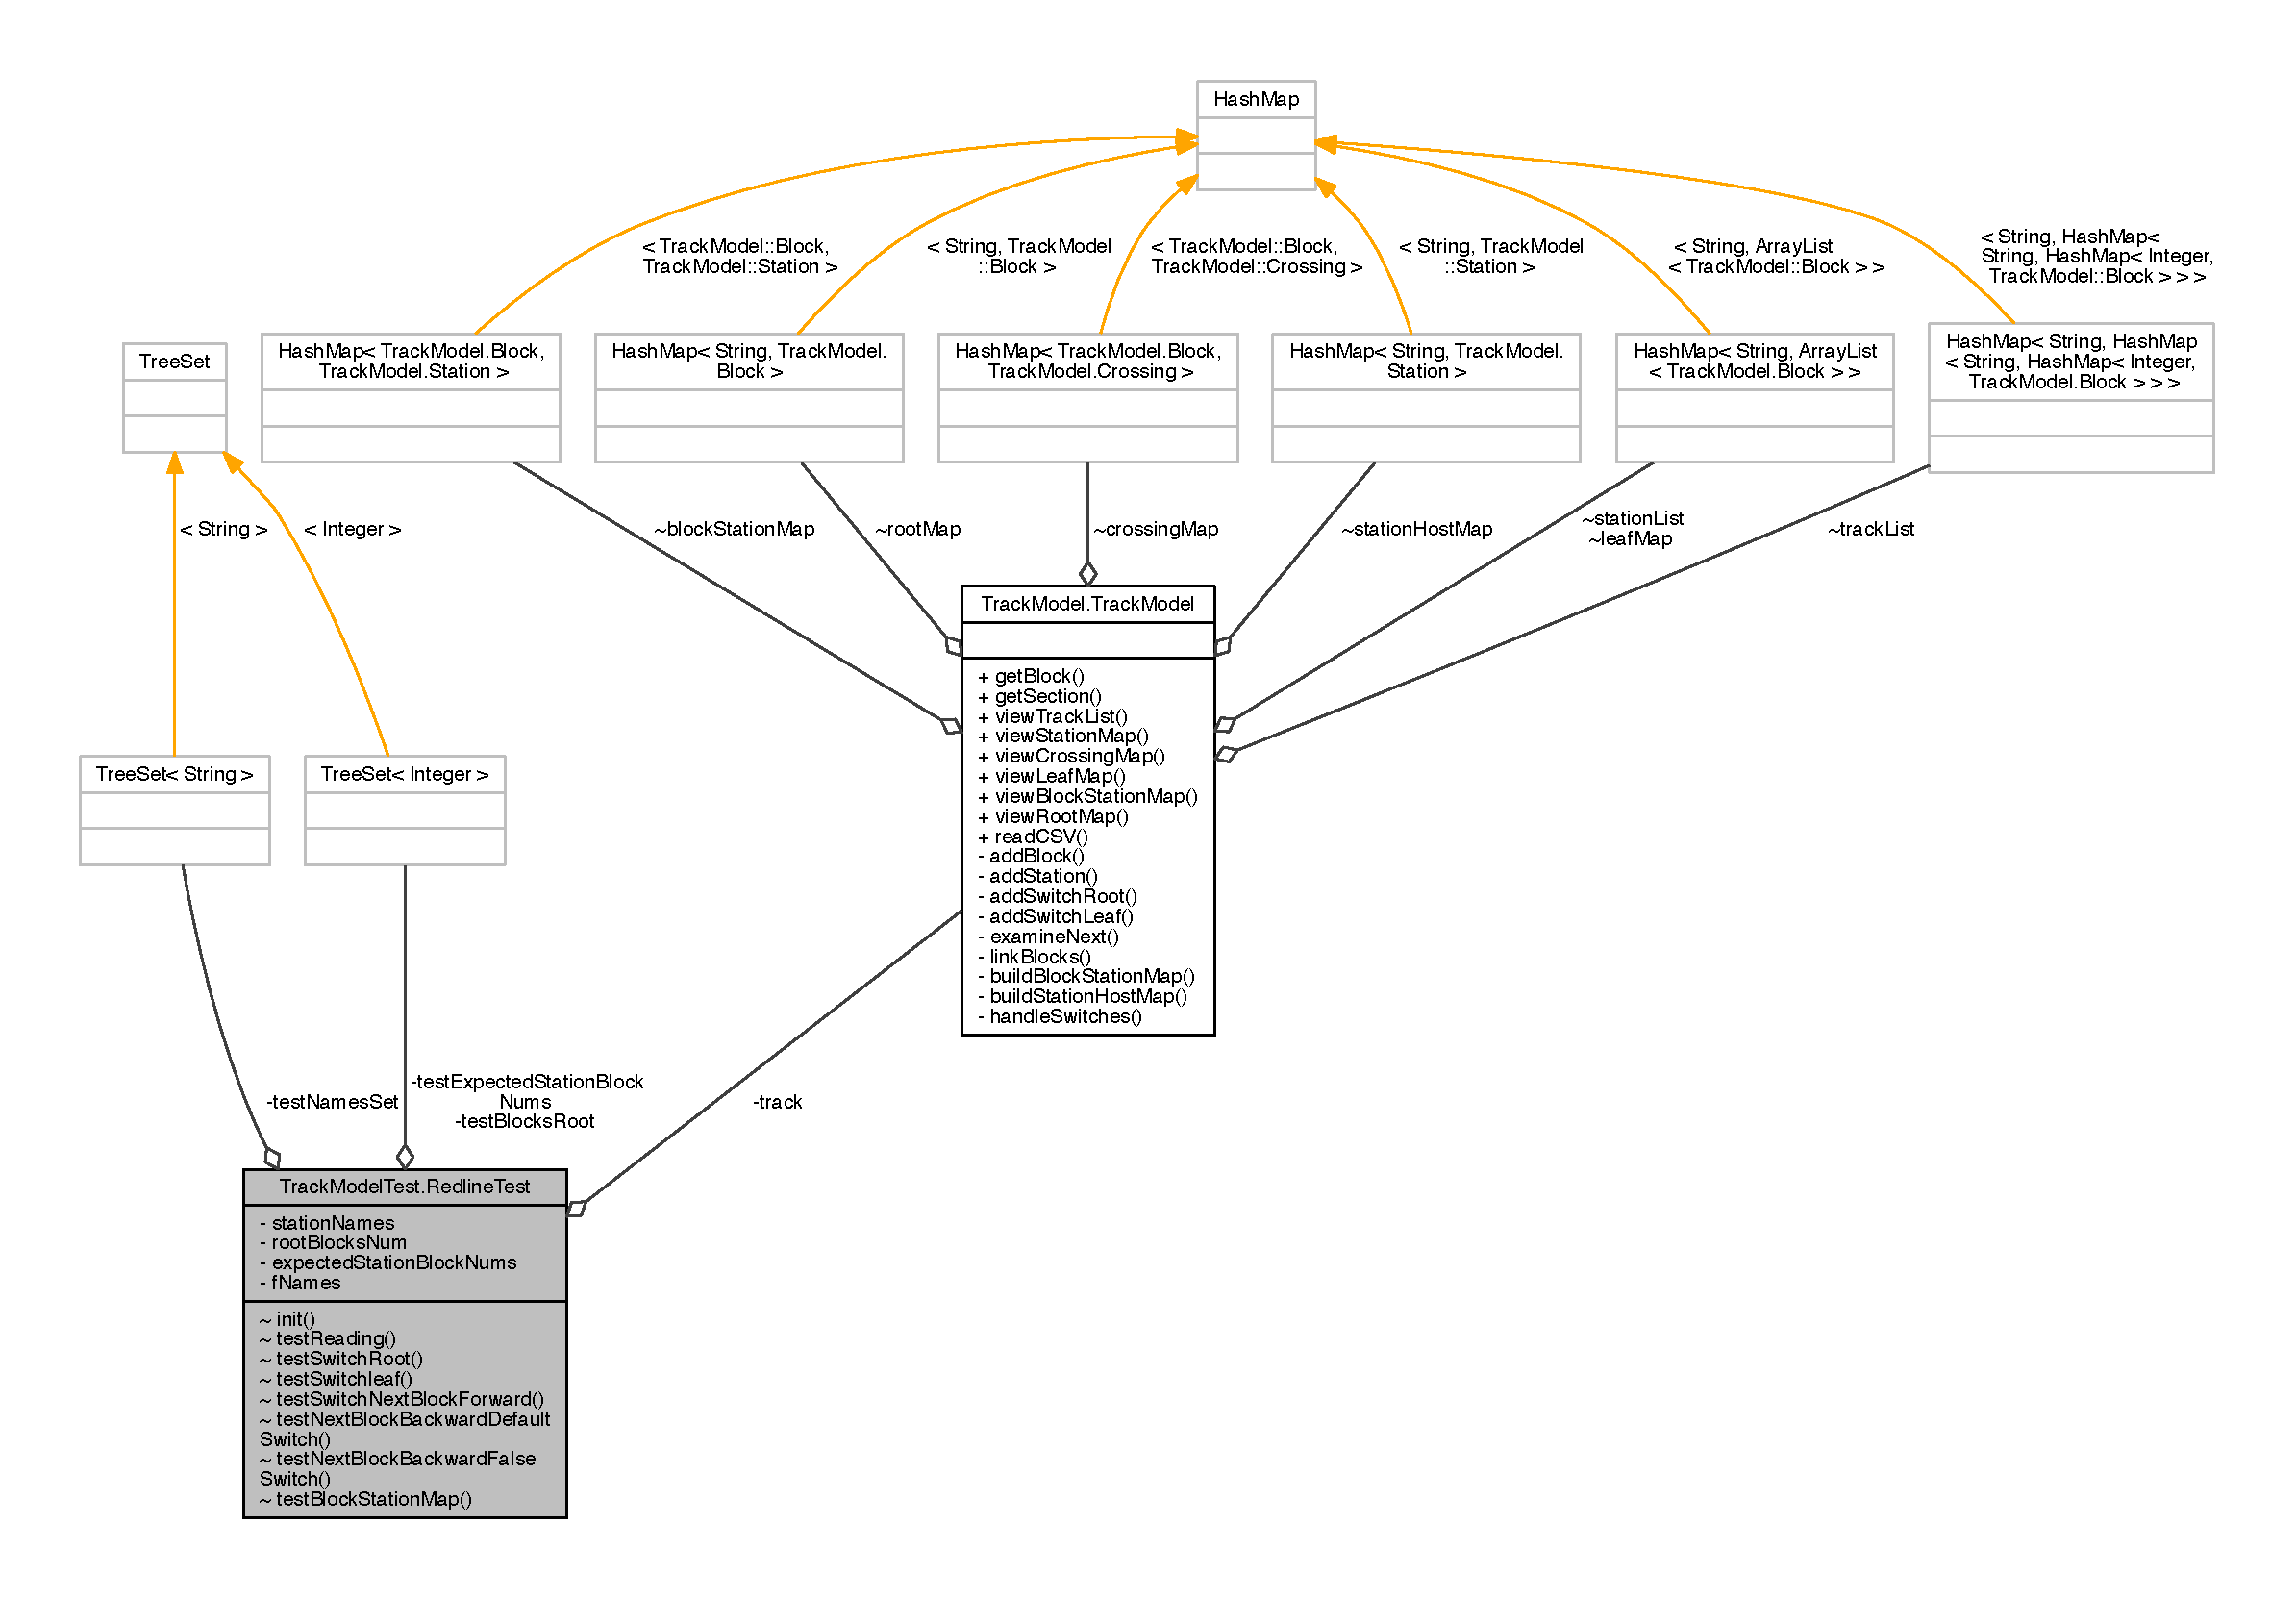
\includegraphics[width=350pt]{classTrackModelTest_1_1RedlineTest__coll__graph}
\end{center}
\end{figure}
\subsection*{Package Functions}
\begin{DoxyCompactItemize}
\item 
void \hyperlink{classTrackModelTest_1_1RedlineTest_a497f6628deb6bfcdacf364347d91a047}{init} ()
\item 
void \hyperlink{classTrackModelTest_1_1RedlineTest_ae4dcd25f8b5aa3ad7b8dc6ba5653fdab}{test\+Reading} ()
\begin{DoxyCompactList}\small\item\em Test for proper station names reading. \end{DoxyCompactList}\item 
void \hyperlink{classTrackModelTest_1_1RedlineTest_a44cf11f1134dd573bb7027a345fdb183}{test\+Switch\+Root} ()
\begin{DoxyCompactList}\small\item\em Test proper block assignment for switch roots. \end{DoxyCompactList}\item 
void \hyperlink{classTrackModelTest_1_1RedlineTest_a8f55cb6090b37b93a36c5af26ea04ed0}{test\+Switchleaf} ()
\begin{DoxyCompactList}\small\item\em Test proper leaf assignments for block on the red line. \end{DoxyCompactList}\item 
void \hyperlink{classTrackModelTest_1_1RedlineTest_a80a489082558d70feb6bcd9e538b259e}{test\+Switch\+Next\+Block\+Forward} ()
\begin{DoxyCompactList}\small\item\em Check proper funcitonality of next\+Block\+Forward by switch state on the red line. \end{DoxyCompactList}\item 
void \hyperlink{classTrackModelTest_1_1RedlineTest_aa09b645d2f4de7e88b8e05e82368a6d6}{test\+Next\+Block\+Backward\+Default\+Switch} ()
\begin{DoxyCompactList}\small\item\em Check testing of next block backward on the redline. \end{DoxyCompactList}\item 
void \hyperlink{classTrackModelTest_1_1RedlineTest_a2970dbaa3e66e82f5e1c6881dae59112}{test\+Next\+Block\+Backward\+False\+Switch} ()
\begin{DoxyCompactList}\small\item\em Check testing of next block backwards on the redline. \end{DoxyCompactList}\item 
void \hyperlink{classTrackModelTest_1_1RedlineTest_a16aa0b2253a86b3b4859ebadbbfc59bf}{test\+Block\+Station\+Map} ()
\begin{DoxyCompactList}\small\item\em Check the functionality of the external block\+Station map for use in the train model and train controller. \end{DoxyCompactList}\end{DoxyCompactItemize}
\subsection*{Static Private Attributes}
\begin{DoxyCompactItemize}
\item 
static String \mbox{[}$\,$\mbox{]} \hyperlink{classTrackModelTest_1_1RedlineTest_af522bafd02e8cc4d845420fd692d3d9b}{station\+Names}
\item 
static Integer \mbox{[}$\,$\mbox{]} \hyperlink{classTrackModelTest_1_1RedlineTest_af6c0d104a6e4c99a443aa92e20b1bc1c}{root\+Blocks\+Num} =\{16,27,33,38,44,52,9\}
\item 
static Integer \mbox{[}$\,$\mbox{]} \hyperlink{classTrackModelTest_1_1RedlineTest_a15b5dcba3d2f7800a07015dfa3a3c015}{expected\+Station\+Block\+Nums} =\{7,9,16,21,25,35,45,48,60\}
\item 
static Tree\+Set$<$ Integer $>$ \hyperlink{classTrackModelTest_1_1RedlineTest_a1e7bd5c2798ce063604fc6738103b5e0}{test\+Blocks\+Root} = new Tree\+Set$<$$>$(Arrays.\+as\+List(\hyperlink{classTrackModelTest_1_1RedlineTest_af6c0d104a6e4c99a443aa92e20b1bc1c}{root\+Blocks\+Num}))
\item 
static Tree\+Set$<$ String $>$ \hyperlink{classTrackModelTest_1_1RedlineTest_a587f6d52dfee441de79812fededfa84b}{test\+Names\+Set} = new Tree\+Set$<$$>$(Arrays.\+as\+List(\hyperlink{classTrackModelTest_1_1RedlineTest_af522bafd02e8cc4d845420fd692d3d9b}{station\+Names}))
\item 
static Tree\+Set$<$ Integer $>$ \hyperlink{classTrackModelTest_1_1RedlineTest_a8a94587a81798044a60016e29a09cd72}{test\+Expected\+Station\+Block\+Nums} = new Tree\+Set$<$$>$(Arrays.\+as\+List(\hyperlink{classTrackModelTest_1_1RedlineTest_a15b5dcba3d2f7800a07015dfa3a3c015}{expected\+Station\+Block\+Nums}))
\item 
static \hyperlink{classTrackModel_1_1TrackModel}{Track\+Model} \hyperlink{classTrackModelTest_1_1RedlineTest_afbab32bc166ca48e7544b8c3908f95e3}{track}
\item 
static String \mbox{[}$\,$\mbox{]} \hyperlink{classTrackModelTest_1_1RedlineTest_a9a9887d39f3d19ee5daf4de70339ba33}{f\+Names} = \{\char`\"{}src/test/resources/redline.\+csv\char`\"{}\}
\end{DoxyCompactItemize}


\subsection{Member Function Documentation}
\mbox{\Hypertarget{classTrackModelTest_1_1RedlineTest_a497f6628deb6bfcdacf364347d91a047}\label{classTrackModelTest_1_1RedlineTest_a497f6628deb6bfcdacf364347d91a047}} 
\index{Track\+Model\+Test\+::\+Redline\+Test@{Track\+Model\+Test\+::\+Redline\+Test}!init@{init}}
\index{init@{init}!Track\+Model\+Test\+::\+Redline\+Test@{Track\+Model\+Test\+::\+Redline\+Test}}
\subsubsection{\texorpdfstring{init()}{init()}}
{\footnotesize\ttfamily void Track\+Model\+Test.\+Redline\+Test.\+init (\begin{DoxyParamCaption}{ }\end{DoxyParamCaption})\hspace{0.3cm}{\ttfamily [package]}}

\mbox{\Hypertarget{classTrackModelTest_1_1RedlineTest_a16aa0b2253a86b3b4859ebadbbfc59bf}\label{classTrackModelTest_1_1RedlineTest_a16aa0b2253a86b3b4859ebadbbfc59bf}} 
\index{Track\+Model\+Test\+::\+Redline\+Test@{Track\+Model\+Test\+::\+Redline\+Test}!test\+Block\+Station\+Map@{test\+Block\+Station\+Map}}
\index{test\+Block\+Station\+Map@{test\+Block\+Station\+Map}!Track\+Model\+Test\+::\+Redline\+Test@{Track\+Model\+Test\+::\+Redline\+Test}}
\subsubsection{\texorpdfstring{test\+Block\+Station\+Map()}{testBlockStationMap()}}
{\footnotesize\ttfamily void Track\+Model\+Test.\+Redline\+Test.\+test\+Block\+Station\+Map (\begin{DoxyParamCaption}{ }\end{DoxyParamCaption})\hspace{0.3cm}{\ttfamily [package]}}



Check the functionality of the external block\+Station map for use in the train model and train controller. 

\mbox{\Hypertarget{classTrackModelTest_1_1RedlineTest_aa09b645d2f4de7e88b8e05e82368a6d6}\label{classTrackModelTest_1_1RedlineTest_aa09b645d2f4de7e88b8e05e82368a6d6}} 
\index{Track\+Model\+Test\+::\+Redline\+Test@{Track\+Model\+Test\+::\+Redline\+Test}!test\+Next\+Block\+Backward\+Default\+Switch@{test\+Next\+Block\+Backward\+Default\+Switch}}
\index{test\+Next\+Block\+Backward\+Default\+Switch@{test\+Next\+Block\+Backward\+Default\+Switch}!Track\+Model\+Test\+::\+Redline\+Test@{Track\+Model\+Test\+::\+Redline\+Test}}
\subsubsection{\texorpdfstring{test\+Next\+Block\+Backward\+Default\+Switch()}{testNextBlockBackwardDefaultSwitch()}}
{\footnotesize\ttfamily void Track\+Model\+Test.\+Redline\+Test.\+test\+Next\+Block\+Backward\+Default\+Switch (\begin{DoxyParamCaption}{ }\end{DoxyParamCaption})\hspace{0.3cm}{\ttfamily [package]}}



Check testing of next block backward on the redline. 

For a \char`\"{}true\char`\"{} (default switch state), the nex\+Block\+Backward should return the root\+Block for the lower indexed block. \mbox{\Hypertarget{classTrackModelTest_1_1RedlineTest_a2970dbaa3e66e82f5e1c6881dae59112}\label{classTrackModelTest_1_1RedlineTest_a2970dbaa3e66e82f5e1c6881dae59112}} 
\index{Track\+Model\+Test\+::\+Redline\+Test@{Track\+Model\+Test\+::\+Redline\+Test}!test\+Next\+Block\+Backward\+False\+Switch@{test\+Next\+Block\+Backward\+False\+Switch}}
\index{test\+Next\+Block\+Backward\+False\+Switch@{test\+Next\+Block\+Backward\+False\+Switch}!Track\+Model\+Test\+::\+Redline\+Test@{Track\+Model\+Test\+::\+Redline\+Test}}
\subsubsection{\texorpdfstring{test\+Next\+Block\+Backward\+False\+Switch()}{testNextBlockBackwardFalseSwitch()}}
{\footnotesize\ttfamily void Track\+Model\+Test.\+Redline\+Test.\+test\+Next\+Block\+Backward\+False\+Switch (\begin{DoxyParamCaption}{ }\end{DoxyParamCaption})\hspace{0.3cm}{\ttfamily [package]}}



Check testing of next block backwards on the redline. 

For a \char`\"{}false\char`\"{} (non-\/default switch state), the next\+Block\+Backward should return the root\+Block for the higher indexed block. \mbox{\Hypertarget{classTrackModelTest_1_1RedlineTest_ae4dcd25f8b5aa3ad7b8dc6ba5653fdab}\label{classTrackModelTest_1_1RedlineTest_ae4dcd25f8b5aa3ad7b8dc6ba5653fdab}} 
\index{Track\+Model\+Test\+::\+Redline\+Test@{Track\+Model\+Test\+::\+Redline\+Test}!test\+Reading@{test\+Reading}}
\index{test\+Reading@{test\+Reading}!Track\+Model\+Test\+::\+Redline\+Test@{Track\+Model\+Test\+::\+Redline\+Test}}
\subsubsection{\texorpdfstring{test\+Reading()}{testReading()}}
{\footnotesize\ttfamily void Track\+Model\+Test.\+Redline\+Test.\+test\+Reading (\begin{DoxyParamCaption}{ }\end{DoxyParamCaption})\hspace{0.3cm}{\ttfamily [package]}}



Test for proper station names reading. 

\mbox{\Hypertarget{classTrackModelTest_1_1RedlineTest_a8f55cb6090b37b93a36c5af26ea04ed0}\label{classTrackModelTest_1_1RedlineTest_a8f55cb6090b37b93a36c5af26ea04ed0}} 
\index{Track\+Model\+Test\+::\+Redline\+Test@{Track\+Model\+Test\+::\+Redline\+Test}!test\+Switchleaf@{test\+Switchleaf}}
\index{test\+Switchleaf@{test\+Switchleaf}!Track\+Model\+Test\+::\+Redline\+Test@{Track\+Model\+Test\+::\+Redline\+Test}}
\subsubsection{\texorpdfstring{test\+Switchleaf()}{testSwitchleaf()}}
{\footnotesize\ttfamily void Track\+Model\+Test.\+Redline\+Test.\+test\+Switchleaf (\begin{DoxyParamCaption}{ }\end{DoxyParamCaption})\hspace{0.3cm}{\ttfamily [package]}}



Test proper leaf assignments for block on the red line. 

\mbox{\Hypertarget{classTrackModelTest_1_1RedlineTest_a80a489082558d70feb6bcd9e538b259e}\label{classTrackModelTest_1_1RedlineTest_a80a489082558d70feb6bcd9e538b259e}} 
\index{Track\+Model\+Test\+::\+Redline\+Test@{Track\+Model\+Test\+::\+Redline\+Test}!test\+Switch\+Next\+Block\+Forward@{test\+Switch\+Next\+Block\+Forward}}
\index{test\+Switch\+Next\+Block\+Forward@{test\+Switch\+Next\+Block\+Forward}!Track\+Model\+Test\+::\+Redline\+Test@{Track\+Model\+Test\+::\+Redline\+Test}}
\subsubsection{\texorpdfstring{test\+Switch\+Next\+Block\+Forward()}{testSwitchNextBlockForward()}}
{\footnotesize\ttfamily void Track\+Model\+Test.\+Redline\+Test.\+test\+Switch\+Next\+Block\+Forward (\begin{DoxyParamCaption}{ }\end{DoxyParamCaption})\hspace{0.3cm}{\ttfamily [package]}}



Check proper funcitonality of next\+Block\+Forward by switch state on the red line. 

\mbox{\Hypertarget{classTrackModelTest_1_1RedlineTest_a44cf11f1134dd573bb7027a345fdb183}\label{classTrackModelTest_1_1RedlineTest_a44cf11f1134dd573bb7027a345fdb183}} 
\index{Track\+Model\+Test\+::\+Redline\+Test@{Track\+Model\+Test\+::\+Redline\+Test}!test\+Switch\+Root@{test\+Switch\+Root}}
\index{test\+Switch\+Root@{test\+Switch\+Root}!Track\+Model\+Test\+::\+Redline\+Test@{Track\+Model\+Test\+::\+Redline\+Test}}
\subsubsection{\texorpdfstring{test\+Switch\+Root()}{testSwitchRoot()}}
{\footnotesize\ttfamily void Track\+Model\+Test.\+Redline\+Test.\+test\+Switch\+Root (\begin{DoxyParamCaption}{ }\end{DoxyParamCaption})\hspace{0.3cm}{\ttfamily [package]}}



Test proper block assignment for switch roots. 



\subsection{Member Data Documentation}
\mbox{\Hypertarget{classTrackModelTest_1_1RedlineTest_a15b5dcba3d2f7800a07015dfa3a3c015}\label{classTrackModelTest_1_1RedlineTest_a15b5dcba3d2f7800a07015dfa3a3c015}} 
\index{Track\+Model\+Test\+::\+Redline\+Test@{Track\+Model\+Test\+::\+Redline\+Test}!expected\+Station\+Block\+Nums@{expected\+Station\+Block\+Nums}}
\index{expected\+Station\+Block\+Nums@{expected\+Station\+Block\+Nums}!Track\+Model\+Test\+::\+Redline\+Test@{Track\+Model\+Test\+::\+Redline\+Test}}
\subsubsection{\texorpdfstring{expected\+Station\+Block\+Nums}{expectedStationBlockNums}}
{\footnotesize\ttfamily Integer \mbox{[}$\,$\mbox{]} Track\+Model\+Test.\+Redline\+Test.\+expected\+Station\+Block\+Nums =\{7,9,16,21,25,35,45,48,60\}\hspace{0.3cm}{\ttfamily [static]}, {\ttfamily [private]}}

\mbox{\Hypertarget{classTrackModelTest_1_1RedlineTest_a9a9887d39f3d19ee5daf4de70339ba33}\label{classTrackModelTest_1_1RedlineTest_a9a9887d39f3d19ee5daf4de70339ba33}} 
\index{Track\+Model\+Test\+::\+Redline\+Test@{Track\+Model\+Test\+::\+Redline\+Test}!f\+Names@{f\+Names}}
\index{f\+Names@{f\+Names}!Track\+Model\+Test\+::\+Redline\+Test@{Track\+Model\+Test\+::\+Redline\+Test}}
\subsubsection{\texorpdfstring{f\+Names}{fNames}}
{\footnotesize\ttfamily String \mbox{[}$\,$\mbox{]} Track\+Model\+Test.\+Redline\+Test.\+f\+Names = \{\char`\"{}src/test/resources/redline.\+csv\char`\"{}\}\hspace{0.3cm}{\ttfamily [static]}, {\ttfamily [private]}}

\mbox{\Hypertarget{classTrackModelTest_1_1RedlineTest_af6c0d104a6e4c99a443aa92e20b1bc1c}\label{classTrackModelTest_1_1RedlineTest_af6c0d104a6e4c99a443aa92e20b1bc1c}} 
\index{Track\+Model\+Test\+::\+Redline\+Test@{Track\+Model\+Test\+::\+Redline\+Test}!root\+Blocks\+Num@{root\+Blocks\+Num}}
\index{root\+Blocks\+Num@{root\+Blocks\+Num}!Track\+Model\+Test\+::\+Redline\+Test@{Track\+Model\+Test\+::\+Redline\+Test}}
\subsubsection{\texorpdfstring{root\+Blocks\+Num}{rootBlocksNum}}
{\footnotesize\ttfamily Integer \mbox{[}$\,$\mbox{]} Track\+Model\+Test.\+Redline\+Test.\+root\+Blocks\+Num =\{16,27,33,38,44,52,9\}\hspace{0.3cm}{\ttfamily [static]}, {\ttfamily [private]}}

\mbox{\Hypertarget{classTrackModelTest_1_1RedlineTest_af522bafd02e8cc4d845420fd692d3d9b}\label{classTrackModelTest_1_1RedlineTest_af522bafd02e8cc4d845420fd692d3d9b}} 
\index{Track\+Model\+Test\+::\+Redline\+Test@{Track\+Model\+Test\+::\+Redline\+Test}!station\+Names@{station\+Names}}
\index{station\+Names@{station\+Names}!Track\+Model\+Test\+::\+Redline\+Test@{Track\+Model\+Test\+::\+Redline\+Test}}
\subsubsection{\texorpdfstring{station\+Names}{stationNames}}
{\footnotesize\ttfamily String \mbox{[}$\,$\mbox{]} Track\+Model\+Test.\+Redline\+Test.\+station\+Names\hspace{0.3cm}{\ttfamily [static]}, {\ttfamily [private]}}

{\bfseries Initial value\+:}
\begin{DoxyCode}
=\{\textcolor{stringliteral}{"YARD"},\textcolor{stringliteral}{"SHADYSIDE"},\textcolor{stringliteral}{"HERRON AVE"},\textcolor{stringliteral}{"SWISSVILLE"},\textcolor{stringliteral}{"PENN STATION"},
                                \textcolor{stringliteral}{"STEEL PLAZA"},\textcolor{stringliteral}{"FIRST AVE"},\textcolor{stringliteral}{"STATION SQUARE"},\textcolor{stringliteral}{"SOUTH HILLS JUNCTION"},\textcolor{stringliteral}{"YARD"}\}
\end{DoxyCode}
\mbox{\Hypertarget{classTrackModelTest_1_1RedlineTest_a1e7bd5c2798ce063604fc6738103b5e0}\label{classTrackModelTest_1_1RedlineTest_a1e7bd5c2798ce063604fc6738103b5e0}} 
\index{Track\+Model\+Test\+::\+Redline\+Test@{Track\+Model\+Test\+::\+Redline\+Test}!test\+Blocks\+Root@{test\+Blocks\+Root}}
\index{test\+Blocks\+Root@{test\+Blocks\+Root}!Track\+Model\+Test\+::\+Redline\+Test@{Track\+Model\+Test\+::\+Redline\+Test}}
\subsubsection{\texorpdfstring{test\+Blocks\+Root}{testBlocksRoot}}
{\footnotesize\ttfamily Tree\+Set$<$Integer$>$ Track\+Model\+Test.\+Redline\+Test.\+test\+Blocks\+Root = new Tree\+Set$<$$>$(Arrays.\+as\+List(\hyperlink{classTrackModelTest_1_1RedlineTest_af6c0d104a6e4c99a443aa92e20b1bc1c}{root\+Blocks\+Num}))\hspace{0.3cm}{\ttfamily [static]}, {\ttfamily [private]}}

\mbox{\Hypertarget{classTrackModelTest_1_1RedlineTest_a8a94587a81798044a60016e29a09cd72}\label{classTrackModelTest_1_1RedlineTest_a8a94587a81798044a60016e29a09cd72}} 
\index{Track\+Model\+Test\+::\+Redline\+Test@{Track\+Model\+Test\+::\+Redline\+Test}!test\+Expected\+Station\+Block\+Nums@{test\+Expected\+Station\+Block\+Nums}}
\index{test\+Expected\+Station\+Block\+Nums@{test\+Expected\+Station\+Block\+Nums}!Track\+Model\+Test\+::\+Redline\+Test@{Track\+Model\+Test\+::\+Redline\+Test}}
\subsubsection{\texorpdfstring{test\+Expected\+Station\+Block\+Nums}{testExpectedStationBlockNums}}
{\footnotesize\ttfamily Tree\+Set$<$Integer$>$ Track\+Model\+Test.\+Redline\+Test.\+test\+Expected\+Station\+Block\+Nums = new Tree\+Set$<$$>$(Arrays.\+as\+List(\hyperlink{classTrackModelTest_1_1RedlineTest_a15b5dcba3d2f7800a07015dfa3a3c015}{expected\+Station\+Block\+Nums}))\hspace{0.3cm}{\ttfamily [static]}, {\ttfamily [private]}}

\mbox{\Hypertarget{classTrackModelTest_1_1RedlineTest_a587f6d52dfee441de79812fededfa84b}\label{classTrackModelTest_1_1RedlineTest_a587f6d52dfee441de79812fededfa84b}} 
\index{Track\+Model\+Test\+::\+Redline\+Test@{Track\+Model\+Test\+::\+Redline\+Test}!test\+Names\+Set@{test\+Names\+Set}}
\index{test\+Names\+Set@{test\+Names\+Set}!Track\+Model\+Test\+::\+Redline\+Test@{Track\+Model\+Test\+::\+Redline\+Test}}
\subsubsection{\texorpdfstring{test\+Names\+Set}{testNamesSet}}
{\footnotesize\ttfamily Tree\+Set$<$String$>$ Track\+Model\+Test.\+Redline\+Test.\+test\+Names\+Set = new Tree\+Set$<$$>$(Arrays.\+as\+List(\hyperlink{classTrackModelTest_1_1RedlineTest_af522bafd02e8cc4d845420fd692d3d9b}{station\+Names}))\hspace{0.3cm}{\ttfamily [static]}, {\ttfamily [private]}}

\mbox{\Hypertarget{classTrackModelTest_1_1RedlineTest_afbab32bc166ca48e7544b8c3908f95e3}\label{classTrackModelTest_1_1RedlineTest_afbab32bc166ca48e7544b8c3908f95e3}} 
\index{Track\+Model\+Test\+::\+Redline\+Test@{Track\+Model\+Test\+::\+Redline\+Test}!track@{track}}
\index{track@{track}!Track\+Model\+Test\+::\+Redline\+Test@{Track\+Model\+Test\+::\+Redline\+Test}}
\subsubsection{\texorpdfstring{track}{track}}
{\footnotesize\ttfamily \hyperlink{classTrackModel_1_1TrackModel}{Track\+Model} Track\+Model\+Test.\+Redline\+Test.\+track\hspace{0.3cm}{\ttfamily [static]}, {\ttfamily [private]}}



The documentation for this class was generated from the following file\+:\begin{DoxyCompactItemize}
\item 
src/test/java/\+Track\+Model\+Test/\hyperlink{RedlineTest_8java}{Redline\+Test.\+java}\end{DoxyCompactItemize}

\hypertarget{classTrackModel_1_1Station}{}\section{Track\+Model.\+Station Class Reference}
\label{classTrackModel_1_1Station}\index{Track\+Model.\+Station@{Track\+Model.\+Station}}


Inheritance diagram for Track\+Model.\+Station\+:
\nopagebreak
\begin{figure}[H]
\begin{center}
\leavevmode
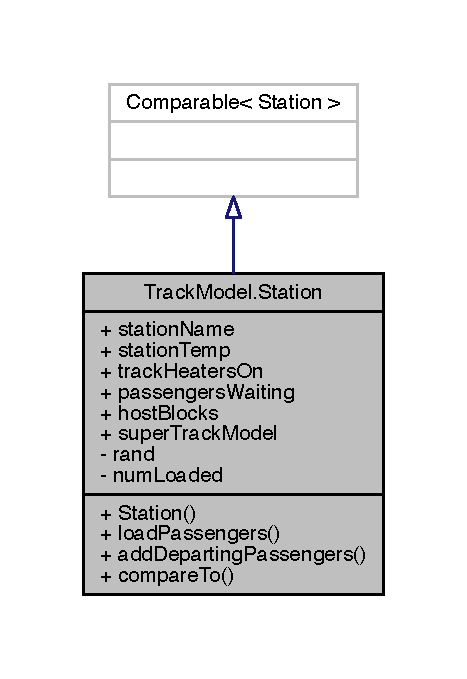
\includegraphics[width=224pt]{classTrackModel_1_1Station__inherit__graph}
\end{center}
\end{figure}


Collaboration diagram for Track\+Model.\+Station\+:
\nopagebreak
\begin{figure}[H]
\begin{center}
\leavevmode
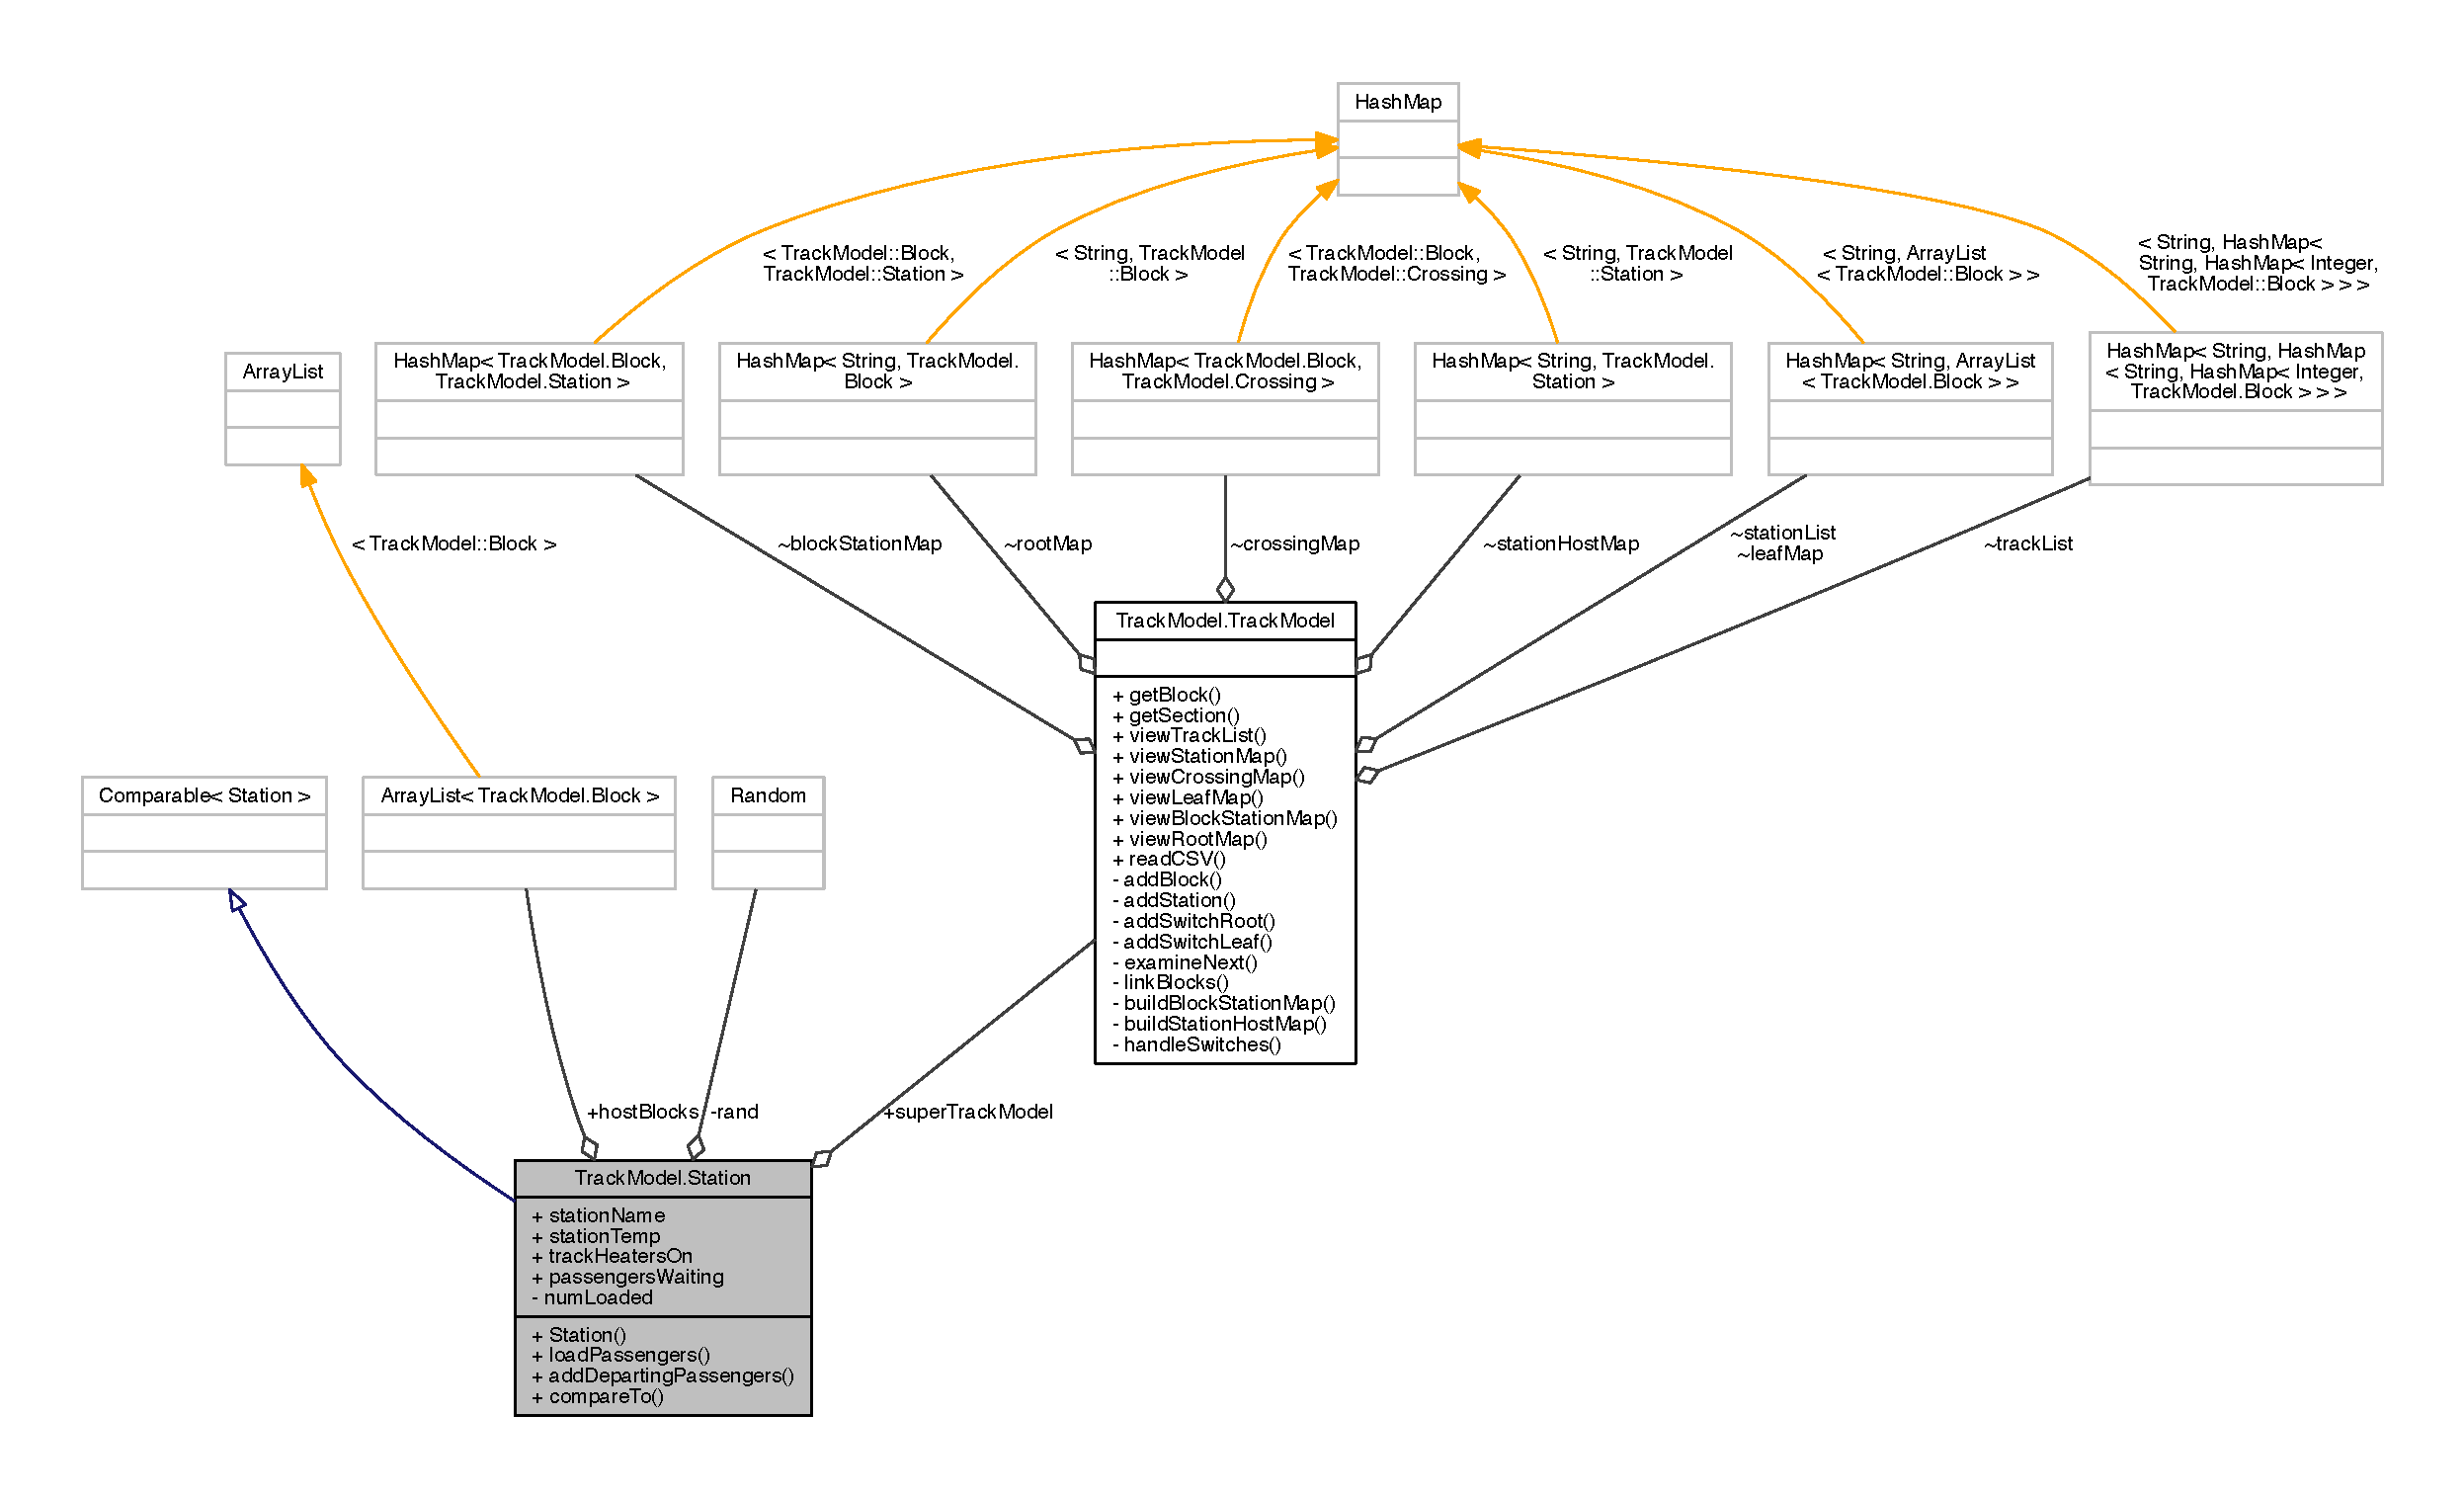
\includegraphics[width=350pt]{classTrackModel_1_1Station__coll__graph}
\end{center}
\end{figure}
\subsection*{Public Member Functions}
\begin{DoxyCompactItemize}
\item 
\hyperlink{classTrackModel_1_1Station_a7eed6cecf5fb632c26a6064494b87ef9}{Station} (String \hyperlink{classTrackModel_1_1Station_ade0b039b51a3d1ff2c2a50dcb8aae373}{station\+Name}, Array\+List$<$ \hyperlink{classTrackModel_1_1Block}{Block} $>$ \hyperlink{classTrackModel_1_1Station_a883b119a2527361b3d1e0bc9d7a8910e}{host\+Blocks})
\item 
Integer \hyperlink{classTrackModel_1_1Station_abba652aa7df49e552eebdc1fa4b1fae7}{load\+Passengers} (Integer max\+Passengers)
\begin{DoxyCompactList}\small\item\em Loads passengers from the waiting area to a train. \end{DoxyCompactList}\item 
void \hyperlink{classTrackModel_1_1Station_a25a87034f554af5c03c420d89e63d3e3}{add\+Departing\+Passengers} (Integer num\+Passengers)
\begin{DoxyCompactList}\small\item\em Adds departing passengers to the waiting area. \end{DoxyCompactList}\item 
int \hyperlink{classTrackModel_1_1Station_adca3eabc08f04c22e9f0f26c93ca9523}{compare\+To} (\hyperlink{classTrackModel_1_1Station}{Station} that\+Station)
\begin{DoxyCompactList}\small\item\em Implements comparable interface for a station based upon the name of a station. \end{DoxyCompactList}\end{DoxyCompactItemize}
\subsection*{Public Attributes}
\begin{DoxyCompactItemize}
\item 
String \hyperlink{classTrackModel_1_1Station_ade0b039b51a3d1ff2c2a50dcb8aae373}{station\+Name}
\item 
Integer \hyperlink{classTrackModel_1_1Station_ac5bcaf08656757e65ce426d4fcf5f8d6}{station\+Temp}
\item 
Boolean \hyperlink{classTrackModel_1_1Station_ae02bb86e9422f05d89f8c3cc52cc21bf}{track\+Heaters\+On}
\item 
Integer \hyperlink{classTrackModel_1_1Station_ae1fd79a5284565937a5b3b04d8e7c12e}{passengers\+Waiting}
\item 
Array\+List$<$ \hyperlink{classTrackModel_1_1Block}{Block} $>$ \hyperlink{classTrackModel_1_1Station_a883b119a2527361b3d1e0bc9d7a8910e}{host\+Blocks}
\item 
\hyperlink{classTrackModel_1_1TrackModel}{Track\+Model} \hyperlink{classTrackModel_1_1Station_aad52bf83bfb9f6c2753e6b0e39c17fc8}{super\+Track\+Model}
\end{DoxyCompactItemize}
\subsection*{Private Attributes}
\begin{DoxyCompactItemize}
\item 
Random \hyperlink{classTrackModel_1_1Station_a2876f95e84690acf90adc1a8714806ed}{rand}
\item 
Integer \hyperlink{classTrackModel_1_1Station_a39b4f364ac4ed45ed0607677245e396d}{num\+Loaded}
\end{DoxyCompactItemize}


\subsection{Constructor \& Destructor Documentation}
\mbox{\Hypertarget{classTrackModel_1_1Station_a7eed6cecf5fb632c26a6064494b87ef9}\label{classTrackModel_1_1Station_a7eed6cecf5fb632c26a6064494b87ef9}} 
\index{Track\+Model\+::\+Station@{Track\+Model\+::\+Station}!Station@{Station}}
\index{Station@{Station}!Track\+Model\+::\+Station@{Track\+Model\+::\+Station}}
\subsubsection{\texorpdfstring{Station()}{Station()}}
{\footnotesize\ttfamily Track\+Model.\+Station.\+Station (\begin{DoxyParamCaption}\item[{String}]{station\+Name,  }\item[{Array\+List$<$ \hyperlink{classTrackModel_1_1Block}{Block} $>$}]{host\+Blocks }\end{DoxyParamCaption})}



\subsection{Member Function Documentation}
\mbox{\Hypertarget{classTrackModel_1_1Station_a25a87034f554af5c03c420d89e63d3e3}\label{classTrackModel_1_1Station_a25a87034f554af5c03c420d89e63d3e3}} 
\index{Track\+Model\+::\+Station@{Track\+Model\+::\+Station}!add\+Departing\+Passengers@{add\+Departing\+Passengers}}
\index{add\+Departing\+Passengers@{add\+Departing\+Passengers}!Track\+Model\+::\+Station@{Track\+Model\+::\+Station}}
\subsubsection{\texorpdfstring{add\+Departing\+Passengers()}{addDepartingPassengers()}}
{\footnotesize\ttfamily void Track\+Model.\+Station.\+add\+Departing\+Passengers (\begin{DoxyParamCaption}\item[{Integer}]{num\+Passengers }\end{DoxyParamCaption})}



Adds departing passengers to the waiting area. 


\begin{DoxyParams}{Parameters}
{\em num\+Passengers} & number of passengers to add to the waiting area \\
\hline
\end{DoxyParams}
\mbox{\Hypertarget{classTrackModel_1_1Station_adca3eabc08f04c22e9f0f26c93ca9523}\label{classTrackModel_1_1Station_adca3eabc08f04c22e9f0f26c93ca9523}} 
\index{Track\+Model\+::\+Station@{Track\+Model\+::\+Station}!compare\+To@{compare\+To}}
\index{compare\+To@{compare\+To}!Track\+Model\+::\+Station@{Track\+Model\+::\+Station}}
\subsubsection{\texorpdfstring{compare\+To()}{compareTo()}}
{\footnotesize\ttfamily int Track\+Model.\+Station.\+compare\+To (\begin{DoxyParamCaption}\item[{\hyperlink{classTrackModel_1_1Station}{Station}}]{that\+Station }\end{DoxyParamCaption})}



Implements comparable interface for a station based upon the name of a station. 


\begin{DoxyParams}{Parameters}
{\em that\+Station} & station to be compared to \\
\hline
\end{DoxyParams}
\mbox{\Hypertarget{classTrackModel_1_1Station_abba652aa7df49e552eebdc1fa4b1fae7}\label{classTrackModel_1_1Station_abba652aa7df49e552eebdc1fa4b1fae7}} 
\index{Track\+Model\+::\+Station@{Track\+Model\+::\+Station}!load\+Passengers@{load\+Passengers}}
\index{load\+Passengers@{load\+Passengers}!Track\+Model\+::\+Station@{Track\+Model\+::\+Station}}
\subsubsection{\texorpdfstring{load\+Passengers()}{loadPassengers()}}
{\footnotesize\ttfamily Integer Track\+Model.\+Station.\+load\+Passengers (\begin{DoxyParamCaption}\item[{Integer}]{max\+Passengers }\end{DoxyParamCaption})}



Loads passengers from the waiting area to a train. 


\begin{DoxyParams}{Parameters}
{\em max\+Passengers} & maximum passengers to be added to a train \\
\hline
\end{DoxyParams}
\begin{DoxyReturn}{Returns}
return value for a number of passengers 
\end{DoxyReturn}


\subsection{Member Data Documentation}
\mbox{\Hypertarget{classTrackModel_1_1Station_a883b119a2527361b3d1e0bc9d7a8910e}\label{classTrackModel_1_1Station_a883b119a2527361b3d1e0bc9d7a8910e}} 
\index{Track\+Model\+::\+Station@{Track\+Model\+::\+Station}!host\+Blocks@{host\+Blocks}}
\index{host\+Blocks@{host\+Blocks}!Track\+Model\+::\+Station@{Track\+Model\+::\+Station}}
\subsubsection{\texorpdfstring{host\+Blocks}{hostBlocks}}
{\footnotesize\ttfamily Array\+List$<$\hyperlink{classTrackModel_1_1Block}{Block}$>$ Track\+Model.\+Station.\+host\+Blocks}

\mbox{\Hypertarget{classTrackModel_1_1Station_a39b4f364ac4ed45ed0607677245e396d}\label{classTrackModel_1_1Station_a39b4f364ac4ed45ed0607677245e396d}} 
\index{Track\+Model\+::\+Station@{Track\+Model\+::\+Station}!num\+Loaded@{num\+Loaded}}
\index{num\+Loaded@{num\+Loaded}!Track\+Model\+::\+Station@{Track\+Model\+::\+Station}}
\subsubsection{\texorpdfstring{num\+Loaded}{numLoaded}}
{\footnotesize\ttfamily Integer Track\+Model.\+Station.\+num\+Loaded\hspace{0.3cm}{\ttfamily [private]}}

\mbox{\Hypertarget{classTrackModel_1_1Station_ae1fd79a5284565937a5b3b04d8e7c12e}\label{classTrackModel_1_1Station_ae1fd79a5284565937a5b3b04d8e7c12e}} 
\index{Track\+Model\+::\+Station@{Track\+Model\+::\+Station}!passengers\+Waiting@{passengers\+Waiting}}
\index{passengers\+Waiting@{passengers\+Waiting}!Track\+Model\+::\+Station@{Track\+Model\+::\+Station}}
\subsubsection{\texorpdfstring{passengers\+Waiting}{passengersWaiting}}
{\footnotesize\ttfamily Integer Track\+Model.\+Station.\+passengers\+Waiting}

\mbox{\Hypertarget{classTrackModel_1_1Station_a2876f95e84690acf90adc1a8714806ed}\label{classTrackModel_1_1Station_a2876f95e84690acf90adc1a8714806ed}} 
\index{Track\+Model\+::\+Station@{Track\+Model\+::\+Station}!rand@{rand}}
\index{rand@{rand}!Track\+Model\+::\+Station@{Track\+Model\+::\+Station}}
\subsubsection{\texorpdfstring{rand}{rand}}
{\footnotesize\ttfamily Random Track\+Model.\+Station.\+rand\hspace{0.3cm}{\ttfamily [private]}}

\mbox{\Hypertarget{classTrackModel_1_1Station_ade0b039b51a3d1ff2c2a50dcb8aae373}\label{classTrackModel_1_1Station_ade0b039b51a3d1ff2c2a50dcb8aae373}} 
\index{Track\+Model\+::\+Station@{Track\+Model\+::\+Station}!station\+Name@{station\+Name}}
\index{station\+Name@{station\+Name}!Track\+Model\+::\+Station@{Track\+Model\+::\+Station}}
\subsubsection{\texorpdfstring{station\+Name}{stationName}}
{\footnotesize\ttfamily String Track\+Model.\+Station.\+station\+Name}

\mbox{\Hypertarget{classTrackModel_1_1Station_ac5bcaf08656757e65ce426d4fcf5f8d6}\label{classTrackModel_1_1Station_ac5bcaf08656757e65ce426d4fcf5f8d6}} 
\index{Track\+Model\+::\+Station@{Track\+Model\+::\+Station}!station\+Temp@{station\+Temp}}
\index{station\+Temp@{station\+Temp}!Track\+Model\+::\+Station@{Track\+Model\+::\+Station}}
\subsubsection{\texorpdfstring{station\+Temp}{stationTemp}}
{\footnotesize\ttfamily Integer Track\+Model.\+Station.\+station\+Temp}

\mbox{\Hypertarget{classTrackModel_1_1Station_aad52bf83bfb9f6c2753e6b0e39c17fc8}\label{classTrackModel_1_1Station_aad52bf83bfb9f6c2753e6b0e39c17fc8}} 
\index{Track\+Model\+::\+Station@{Track\+Model\+::\+Station}!super\+Track\+Model@{super\+Track\+Model}}
\index{super\+Track\+Model@{super\+Track\+Model}!Track\+Model\+::\+Station@{Track\+Model\+::\+Station}}
\subsubsection{\texorpdfstring{super\+Track\+Model}{superTrackModel}}
{\footnotesize\ttfamily \hyperlink{classTrackModel_1_1TrackModel}{Track\+Model} Track\+Model.\+Station.\+super\+Track\+Model}

\mbox{\Hypertarget{classTrackModel_1_1Station_ae02bb86e9422f05d89f8c3cc52cc21bf}\label{classTrackModel_1_1Station_ae02bb86e9422f05d89f8c3cc52cc21bf}} 
\index{Track\+Model\+::\+Station@{Track\+Model\+::\+Station}!track\+Heaters\+On@{track\+Heaters\+On}}
\index{track\+Heaters\+On@{track\+Heaters\+On}!Track\+Model\+::\+Station@{Track\+Model\+::\+Station}}
\subsubsection{\texorpdfstring{track\+Heaters\+On}{trackHeatersOn}}
{\footnotesize\ttfamily Boolean Track\+Model.\+Station.\+track\+Heaters\+On}



The documentation for this class was generated from the following file\+:\begin{DoxyCompactItemize}
\item 
src/main/java/\+Track\+Model/\hyperlink{Station_8java}{Station.\+java}\end{DoxyCompactItemize}

\hypertarget{classTrainControllerComps_1_1TCBlockInfoPanel}{}\section{Train\+Controller\+Comps.\+T\+C\+Block\+Info\+Panel Class Reference}
\label{classTrainControllerComps_1_1TCBlockInfoPanel}\index{Train\+Controller\+Comps.\+T\+C\+Block\+Info\+Panel@{Train\+Controller\+Comps.\+T\+C\+Block\+Info\+Panel}}


This class is responsible for displaying information regarding the block the selected train is currently in.  




Inheritance diagram for Train\+Controller\+Comps.\+T\+C\+Block\+Info\+Panel\+:
\nopagebreak
\begin{figure}[H]
\begin{center}
\leavevmode
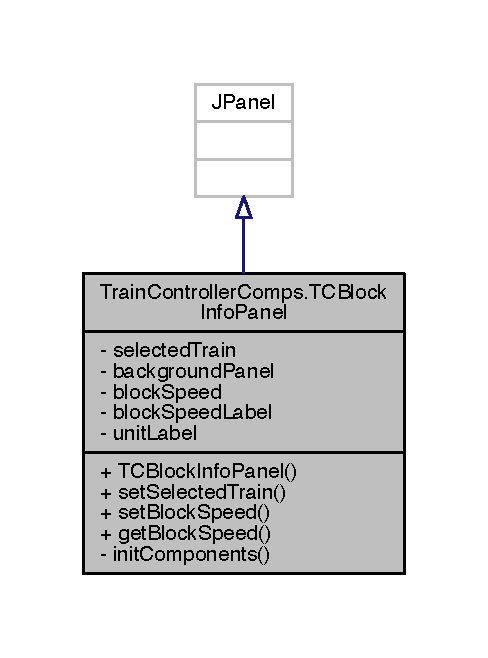
\includegraphics[width=234pt]{classTrainControllerComps_1_1TCBlockInfoPanel__inherit__graph}
\end{center}
\end{figure}


Collaboration diagram for Train\+Controller\+Comps.\+T\+C\+Block\+Info\+Panel\+:
\nopagebreak
\begin{figure}[H]
\begin{center}
\leavevmode
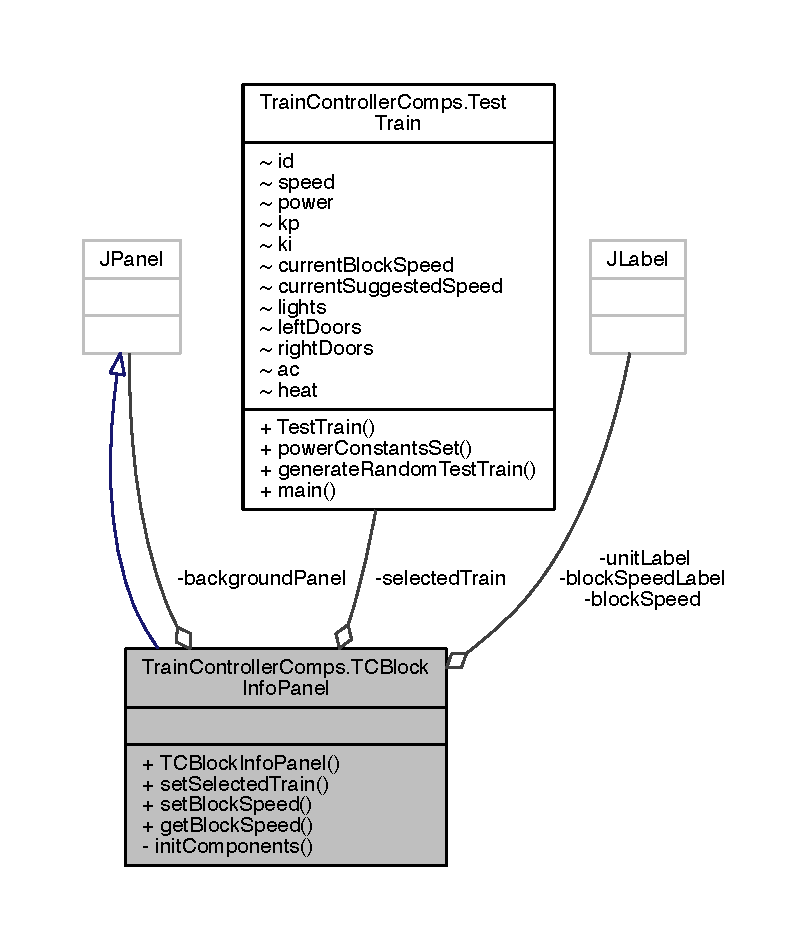
\includegraphics[width=350pt]{classTrainControllerComps_1_1TCBlockInfoPanel__coll__graph}
\end{center}
\end{figure}
\subsection*{Public Member Functions}
\begin{DoxyCompactItemize}
\item 
\hyperlink{classTrainControllerComps_1_1TCBlockInfoPanel_a44a1b4c66f0a95faae3698b9a37cd71c}{T\+C\+Block\+Info\+Panel} ()
\begin{DoxyCompactList}\small\item\em Constructor for a \hyperlink{classTrainControllerComps_1_1TCBlockInfoPanel}{T\+C\+Block\+Info\+Panel} object. \end{DoxyCompactList}\item 
void \hyperlink{classTrainControllerComps_1_1TCBlockInfoPanel_a930f11785e7efa17ccc8909d885de1c5}{set\+Selected\+Train} (\hyperlink{classTrainControllerComps_1_1TestTrain}{Test\+Train} \hyperlink{classtrain}{train})
\begin{DoxyCompactList}\small\item\em Sets the selected train that the class will get its information from. \end{DoxyCompactList}\item 
void \hyperlink{classTrainControllerComps_1_1TCBlockInfoPanel_a2579f1bf5addf760f020e222f831b35a}{set\+Block\+Speed} (double \hyperlink{classTrainControllerComps_1_1TCBlockInfoPanel_a3b3aa9808843291162c5f169c7aea308}{block\+Speed})
\begin{DoxyCompactList}\small\item\em Sets the block speed label to a specified speed in M\+PH. \end{DoxyCompactList}\item 
double \hyperlink{classTrainControllerComps_1_1TCBlockInfoPanel_af6abb156c9e61d36d7fd3d8cb8c899f6}{get\+Block\+Speed} ()
\begin{DoxyCompactList}\small\item\em Gets the speed of the block the selected train is in. \end{DoxyCompactList}\end{DoxyCompactItemize}
\subsection*{Private Member Functions}
\begin{DoxyCompactItemize}
\item 
void \hyperlink{classTrainControllerComps_1_1TCBlockInfoPanel_a0bbafa154ac2cdc3b83140374e85ed25}{init\+Components} ()
\begin{DoxyCompactList}\small\item\em This method is called from within the constructor to initialize the form. \end{DoxyCompactList}\end{DoxyCompactItemize}
\subsection*{Private Attributes}
\begin{DoxyCompactItemize}
\item 
\hyperlink{classTrainControllerComps_1_1TestTrain}{Test\+Train} \hyperlink{classTrainControllerComps_1_1TCBlockInfoPanel_a26dda8277000855ca35d16e6bdb97665}{selected\+Train}
\begin{DoxyCompactList}\small\item\em The train to use in order to populate the labels and UI elements. \end{DoxyCompactList}\item 
javax.\+swing.\+J\+Panel \hyperlink{classTrainControllerComps_1_1TCBlockInfoPanel_a6a9c969b6131a6e6f3d01fd2a9434d6d}{background\+Panel}
\item 
javax.\+swing.\+J\+Label \hyperlink{classTrainControllerComps_1_1TCBlockInfoPanel_a3b3aa9808843291162c5f169c7aea308}{block\+Speed}
\item 
javax.\+swing.\+J\+Label \hyperlink{classTrainControllerComps_1_1TCBlockInfoPanel_a4e08f23bf589fc1e8b361f7473f54127}{block\+Speed\+Label}
\item 
javax.\+swing.\+J\+Label \hyperlink{classTrainControllerComps_1_1TCBlockInfoPanel_a6038128e0c97c299a84e81d8e77b6215}{unit\+Label}
\end{DoxyCompactItemize}


\subsection{Detailed Description}
This class is responsible for displaying information regarding the block the selected train is currently in. 

This class collaborates with the Train class as well as the Train Controller class.

\begin{DoxyAuthor}{Author}
Andrew Lendacky 
\end{DoxyAuthor}


\subsection{Constructor \& Destructor Documentation}
\mbox{\Hypertarget{classTrainControllerComps_1_1TCBlockInfoPanel_a44a1b4c66f0a95faae3698b9a37cd71c}\label{classTrainControllerComps_1_1TCBlockInfoPanel_a44a1b4c66f0a95faae3698b9a37cd71c}} 
\index{Train\+Controller\+Comps\+::\+T\+C\+Block\+Info\+Panel@{Train\+Controller\+Comps\+::\+T\+C\+Block\+Info\+Panel}!T\+C\+Block\+Info\+Panel@{T\+C\+Block\+Info\+Panel}}
\index{T\+C\+Block\+Info\+Panel@{T\+C\+Block\+Info\+Panel}!Train\+Controller\+Comps\+::\+T\+C\+Block\+Info\+Panel@{Train\+Controller\+Comps\+::\+T\+C\+Block\+Info\+Panel}}
\subsubsection{\texorpdfstring{T\+C\+Block\+Info\+Panel()}{TCBlockInfoPanel()}}
{\footnotesize\ttfamily Train\+Controller\+Comps.\+T\+C\+Block\+Info\+Panel.\+T\+C\+Block\+Info\+Panel (\begin{DoxyParamCaption}{ }\end{DoxyParamCaption})}



Constructor for a \hyperlink{classTrainControllerComps_1_1TCBlockInfoPanel}{T\+C\+Block\+Info\+Panel} object. 

This constructor does not set the selected train, and must be set by the Train Controller before being used. 

\subsection{Member Function Documentation}
\mbox{\Hypertarget{classTrainControllerComps_1_1TCBlockInfoPanel_af6abb156c9e61d36d7fd3d8cb8c899f6}\label{classTrainControllerComps_1_1TCBlockInfoPanel_af6abb156c9e61d36d7fd3d8cb8c899f6}} 
\index{Train\+Controller\+Comps\+::\+T\+C\+Block\+Info\+Panel@{Train\+Controller\+Comps\+::\+T\+C\+Block\+Info\+Panel}!get\+Block\+Speed@{get\+Block\+Speed}}
\index{get\+Block\+Speed@{get\+Block\+Speed}!Train\+Controller\+Comps\+::\+T\+C\+Block\+Info\+Panel@{Train\+Controller\+Comps\+::\+T\+C\+Block\+Info\+Panel}}
\subsubsection{\texorpdfstring{get\+Block\+Speed()}{getBlockSpeed()}}
{\footnotesize\ttfamily double Train\+Controller\+Comps.\+T\+C\+Block\+Info\+Panel.\+get\+Block\+Speed (\begin{DoxyParamCaption}{ }\end{DoxyParamCaption})}



Gets the speed of the block the selected train is in. 

\begin{DoxyReturn}{Returns}
returns the block speed 
\end{DoxyReturn}
\mbox{\Hypertarget{classTrainControllerComps_1_1TCBlockInfoPanel_a0bbafa154ac2cdc3b83140374e85ed25}\label{classTrainControllerComps_1_1TCBlockInfoPanel_a0bbafa154ac2cdc3b83140374e85ed25}} 
\index{Train\+Controller\+Comps\+::\+T\+C\+Block\+Info\+Panel@{Train\+Controller\+Comps\+::\+T\+C\+Block\+Info\+Panel}!init\+Components@{init\+Components}}
\index{init\+Components@{init\+Components}!Train\+Controller\+Comps\+::\+T\+C\+Block\+Info\+Panel@{Train\+Controller\+Comps\+::\+T\+C\+Block\+Info\+Panel}}
\subsubsection{\texorpdfstring{init\+Components()}{initComponents()}}
{\footnotesize\ttfamily void Train\+Controller\+Comps.\+T\+C\+Block\+Info\+Panel.\+init\+Components (\begin{DoxyParamCaption}{ }\end{DoxyParamCaption})\hspace{0.3cm}{\ttfamily [private]}}



This method is called from within the constructor to initialize the form. 

W\+A\+R\+N\+I\+NG\+: Do N\+OT modify this code. The content of this method is always regenerated by the Form Editor. \mbox{\Hypertarget{classTrainControllerComps_1_1TCBlockInfoPanel_a2579f1bf5addf760f020e222f831b35a}\label{classTrainControllerComps_1_1TCBlockInfoPanel_a2579f1bf5addf760f020e222f831b35a}} 
\index{Train\+Controller\+Comps\+::\+T\+C\+Block\+Info\+Panel@{Train\+Controller\+Comps\+::\+T\+C\+Block\+Info\+Panel}!set\+Block\+Speed@{set\+Block\+Speed}}
\index{set\+Block\+Speed@{set\+Block\+Speed}!Train\+Controller\+Comps\+::\+T\+C\+Block\+Info\+Panel@{Train\+Controller\+Comps\+::\+T\+C\+Block\+Info\+Panel}}
\subsubsection{\texorpdfstring{set\+Block\+Speed()}{setBlockSpeed()}}
{\footnotesize\ttfamily void Train\+Controller\+Comps.\+T\+C\+Block\+Info\+Panel.\+set\+Block\+Speed (\begin{DoxyParamCaption}\item[{double}]{block\+Speed }\end{DoxyParamCaption})}



Sets the block speed label to a specified speed in M\+PH. 


\begin{DoxyParams}{Parameters}
{\em block\+Speed} & the speed of the block the train is in. \\
\hline
\end{DoxyParams}
\mbox{\Hypertarget{classTrainControllerComps_1_1TCBlockInfoPanel_a930f11785e7efa17ccc8909d885de1c5}\label{classTrainControllerComps_1_1TCBlockInfoPanel_a930f11785e7efa17ccc8909d885de1c5}} 
\index{Train\+Controller\+Comps\+::\+T\+C\+Block\+Info\+Panel@{Train\+Controller\+Comps\+::\+T\+C\+Block\+Info\+Panel}!set\+Selected\+Train@{set\+Selected\+Train}}
\index{set\+Selected\+Train@{set\+Selected\+Train}!Train\+Controller\+Comps\+::\+T\+C\+Block\+Info\+Panel@{Train\+Controller\+Comps\+::\+T\+C\+Block\+Info\+Panel}}
\subsubsection{\texorpdfstring{set\+Selected\+Train()}{setSelectedTrain()}}
{\footnotesize\ttfamily void Train\+Controller\+Comps.\+T\+C\+Block\+Info\+Panel.\+set\+Selected\+Train (\begin{DoxyParamCaption}\item[{\hyperlink{classTrainControllerComps_1_1TestTrain}{Test\+Train}}]{train }\end{DoxyParamCaption})}



Sets the selected train that the class will get its information from. 

This train is set from the Train Controller class.


\begin{DoxyParams}{Parameters}
{\em train} & the selected train \\
\hline
\end{DoxyParams}


\subsection{Member Data Documentation}
\mbox{\Hypertarget{classTrainControllerComps_1_1TCBlockInfoPanel_a6a9c969b6131a6e6f3d01fd2a9434d6d}\label{classTrainControllerComps_1_1TCBlockInfoPanel_a6a9c969b6131a6e6f3d01fd2a9434d6d}} 
\index{Train\+Controller\+Comps\+::\+T\+C\+Block\+Info\+Panel@{Train\+Controller\+Comps\+::\+T\+C\+Block\+Info\+Panel}!background\+Panel@{background\+Panel}}
\index{background\+Panel@{background\+Panel}!Train\+Controller\+Comps\+::\+T\+C\+Block\+Info\+Panel@{Train\+Controller\+Comps\+::\+T\+C\+Block\+Info\+Panel}}
\subsubsection{\texorpdfstring{background\+Panel}{backgroundPanel}}
{\footnotesize\ttfamily javax.\+swing.\+J\+Panel Train\+Controller\+Comps.\+T\+C\+Block\+Info\+Panel.\+background\+Panel\hspace{0.3cm}{\ttfamily [private]}}

\mbox{\Hypertarget{classTrainControllerComps_1_1TCBlockInfoPanel_a3b3aa9808843291162c5f169c7aea308}\label{classTrainControllerComps_1_1TCBlockInfoPanel_a3b3aa9808843291162c5f169c7aea308}} 
\index{Train\+Controller\+Comps\+::\+T\+C\+Block\+Info\+Panel@{Train\+Controller\+Comps\+::\+T\+C\+Block\+Info\+Panel}!block\+Speed@{block\+Speed}}
\index{block\+Speed@{block\+Speed}!Train\+Controller\+Comps\+::\+T\+C\+Block\+Info\+Panel@{Train\+Controller\+Comps\+::\+T\+C\+Block\+Info\+Panel}}
\subsubsection{\texorpdfstring{block\+Speed}{blockSpeed}}
{\footnotesize\ttfamily javax.\+swing.\+J\+Label Train\+Controller\+Comps.\+T\+C\+Block\+Info\+Panel.\+block\+Speed\hspace{0.3cm}{\ttfamily [private]}}

\mbox{\Hypertarget{classTrainControllerComps_1_1TCBlockInfoPanel_a4e08f23bf589fc1e8b361f7473f54127}\label{classTrainControllerComps_1_1TCBlockInfoPanel_a4e08f23bf589fc1e8b361f7473f54127}} 
\index{Train\+Controller\+Comps\+::\+T\+C\+Block\+Info\+Panel@{Train\+Controller\+Comps\+::\+T\+C\+Block\+Info\+Panel}!block\+Speed\+Label@{block\+Speed\+Label}}
\index{block\+Speed\+Label@{block\+Speed\+Label}!Train\+Controller\+Comps\+::\+T\+C\+Block\+Info\+Panel@{Train\+Controller\+Comps\+::\+T\+C\+Block\+Info\+Panel}}
\subsubsection{\texorpdfstring{block\+Speed\+Label}{blockSpeedLabel}}
{\footnotesize\ttfamily javax.\+swing.\+J\+Label Train\+Controller\+Comps.\+T\+C\+Block\+Info\+Panel.\+block\+Speed\+Label\hspace{0.3cm}{\ttfamily [private]}}

\mbox{\Hypertarget{classTrainControllerComps_1_1TCBlockInfoPanel_a26dda8277000855ca35d16e6bdb97665}\label{classTrainControllerComps_1_1TCBlockInfoPanel_a26dda8277000855ca35d16e6bdb97665}} 
\index{Train\+Controller\+Comps\+::\+T\+C\+Block\+Info\+Panel@{Train\+Controller\+Comps\+::\+T\+C\+Block\+Info\+Panel}!selected\+Train@{selected\+Train}}
\index{selected\+Train@{selected\+Train}!Train\+Controller\+Comps\+::\+T\+C\+Block\+Info\+Panel@{Train\+Controller\+Comps\+::\+T\+C\+Block\+Info\+Panel}}
\subsubsection{\texorpdfstring{selected\+Train}{selectedTrain}}
{\footnotesize\ttfamily \hyperlink{classTrainControllerComps_1_1TestTrain}{Test\+Train} Train\+Controller\+Comps.\+T\+C\+Block\+Info\+Panel.\+selected\+Train\hspace{0.3cm}{\ttfamily [private]}}



The train to use in order to populate the labels and UI elements. 

This property must be passed in from the Train Controller class. \mbox{\Hypertarget{classTrainControllerComps_1_1TCBlockInfoPanel_a6038128e0c97c299a84e81d8e77b6215}\label{classTrainControllerComps_1_1TCBlockInfoPanel_a6038128e0c97c299a84e81d8e77b6215}} 
\index{Train\+Controller\+Comps\+::\+T\+C\+Block\+Info\+Panel@{Train\+Controller\+Comps\+::\+T\+C\+Block\+Info\+Panel}!unit\+Label@{unit\+Label}}
\index{unit\+Label@{unit\+Label}!Train\+Controller\+Comps\+::\+T\+C\+Block\+Info\+Panel@{Train\+Controller\+Comps\+::\+T\+C\+Block\+Info\+Panel}}
\subsubsection{\texorpdfstring{unit\+Label}{unitLabel}}
{\footnotesize\ttfamily javax.\+swing.\+J\+Label Train\+Controller\+Comps.\+T\+C\+Block\+Info\+Panel.\+unit\+Label\hspace{0.3cm}{\ttfamily [private]}}



The documentation for this class was generated from the following file\+:\begin{DoxyCompactItemize}
\item 
src/main/java/\+Train\+Controller\+Comps/\hyperlink{TCBlockInfoPanel_8java}{T\+C\+Block\+Info\+Panel.\+java}\end{DoxyCompactItemize}

\hypertarget{classTrainControllerComps_1_1TCBrakePanel}{}\section{Train\+Controller\+Comps.\+T\+C\+Brake\+Panel Class Reference}
\label{classTrainControllerComps_1_1TCBrakePanel}\index{Train\+Controller\+Comps.\+T\+C\+Brake\+Panel@{Train\+Controller\+Comps.\+T\+C\+Brake\+Panel}}


This class is responsible for applying and managing the use of a train\textquotesingle{}s braking system.  




Inheritance diagram for Train\+Controller\+Comps.\+T\+C\+Brake\+Panel\+:
\nopagebreak
\begin{figure}[H]
\begin{center}
\leavevmode
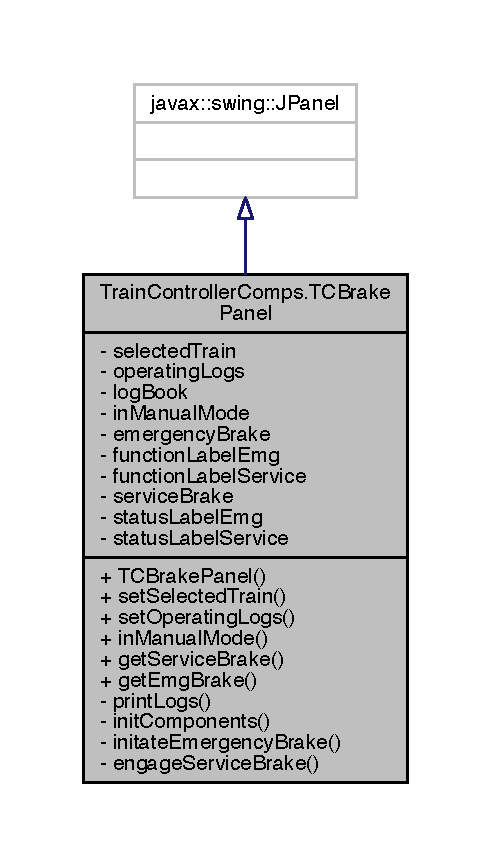
\includegraphics[width=236pt]{classTrainControllerComps_1_1TCBrakePanel__inherit__graph}
\end{center}
\end{figure}


Collaboration diagram for Train\+Controller\+Comps.\+T\+C\+Brake\+Panel\+:
\nopagebreak
\begin{figure}[H]
\begin{center}
\leavevmode
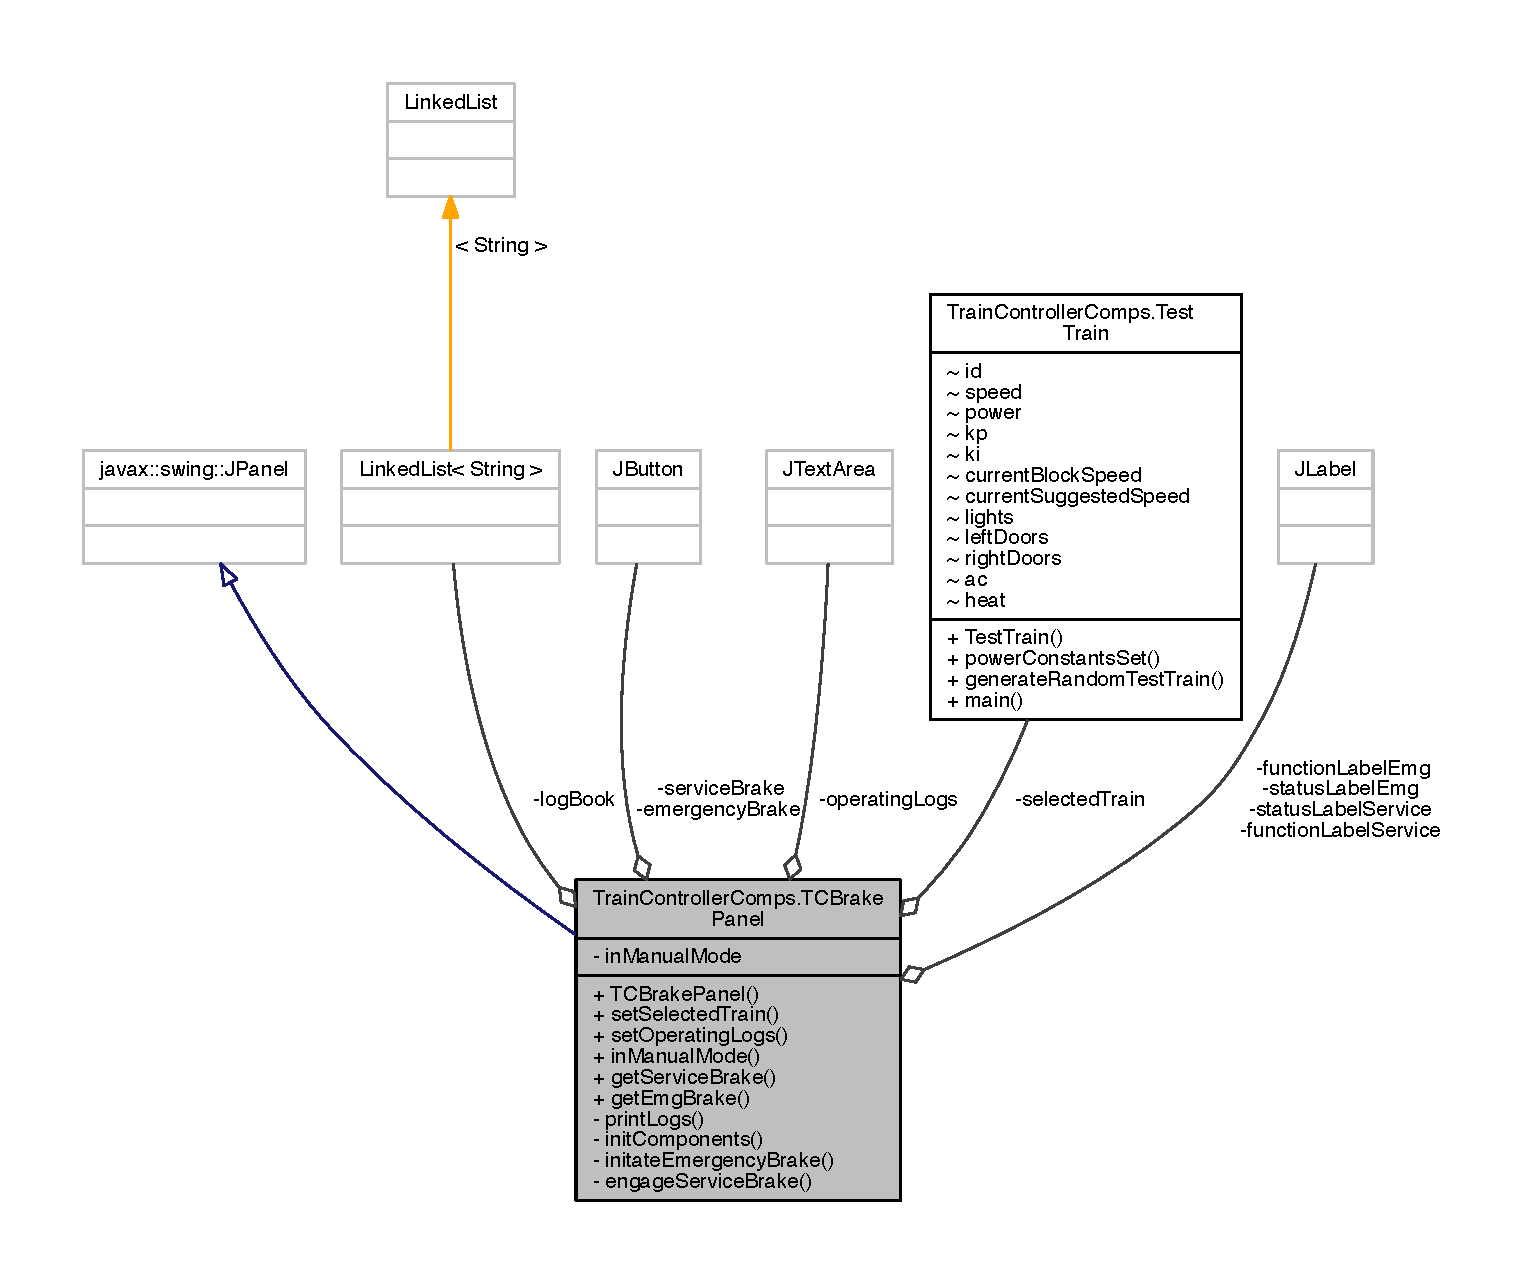
\includegraphics[width=350pt]{classTrainControllerComps_1_1TCBrakePanel__coll__graph}
\end{center}
\end{figure}
\subsection*{Public Member Functions}
\begin{DoxyCompactItemize}
\item 
\hyperlink{classTrainControllerComps_1_1TCBrakePanel_a5940e47f6529fb96044ba90413906b30}{T\+C\+Brake\+Panel} ()
\begin{DoxyCompactList}\small\item\em Constructor for creating a \hyperlink{classTrainControllerComps_1_1TCBrakePanel}{T\+C\+Brake\+Panel} object without a selected train. \end{DoxyCompactList}\item 
void \hyperlink{classTrainControllerComps_1_1TCBrakePanel_a081a9013d44c3933e6acb9a7bd01135f}{set\+Selected\+Train} (\hyperlink{classTrainControllerComps_1_1TestTrain}{Test\+Train} \hyperlink{classTrainControllerComps_1_1TCBrakePanel_ac8f5bb4b6ea27c0d53b99945f9c68141}{selected\+Train})
\begin{DoxyCompactList}\small\item\em Sets the selected train that this class is to control. \end{DoxyCompactList}\item 
void \hyperlink{classTrainControllerComps_1_1TCBrakePanel_ac705fa5eeb5f291ccc8a5af7885fc7c6}{set\+Operating\+Logs} (J\+Text\+Area op\+Logs)
\begin{DoxyCompactList}\small\item\em Sets the text field to be used for the operating logs. \end{DoxyCompactList}\item 
void \hyperlink{classTrainControllerComps_1_1TCBrakePanel_a4ba678ac423a17477b5b15077c55cb7a}{in\+Manual\+Mode} (boolean b)
\begin{DoxyCompactList}\small\item\em Set if the system should be in Manual or Automatic mode. \end{DoxyCompactList}\item 
J\+Button \hyperlink{classTrainControllerComps_1_1TCBrakePanel_af33870de15eae5f27e4cfce85efda275}{get\+Service\+Brake} ()
\begin{DoxyCompactList}\small\item\em Returns the service brake button. \end{DoxyCompactList}\item 
J\+Button \hyperlink{classTrainControllerComps_1_1TCBrakePanel_a1e16cb37e8eecb4d6fc13fbb6f9aa09d}{get\+Emg\+Brake} ()
\begin{DoxyCompactList}\small\item\em Returns the emergency brake button. \end{DoxyCompactList}\end{DoxyCompactItemize}
\subsection*{Private Member Functions}
\begin{DoxyCompactItemize}
\item 
void \hyperlink{classTrainControllerComps_1_1TCBrakePanel_a901968694edba045f8ee6216d89a4096}{print\+Logs} ()
\begin{DoxyCompactList}\small\item\em Prints the messages stored in the logbook to the operating log, then clears the logbook. \end{DoxyCompactList}\item 
void \hyperlink{classTrainControllerComps_1_1TCBrakePanel_a9de925ba11a22e74716c6009d666b0d2}{init\+Components} ()
\begin{DoxyCompactList}\small\item\em This method is called from within the constructor to initialize the form. \end{DoxyCompactList}\item 
void \hyperlink{classTrainControllerComps_1_1TCBrakePanel_a88605d5c8969b8c38af57f077a6289ce}{initate\+Emergency\+Brake} (java.\+awt.\+event.\+Action\+Event evt)
\begin{DoxyCompactList}\small\item\em Initiates the emergency brake on the selected train. \end{DoxyCompactList}\item 
void \hyperlink{classTrainControllerComps_1_1TCBrakePanel_a14938e5fe8d51e9f556097d274fa5b92}{engage\+Service\+Brake} (java.\+awt.\+event.\+Action\+Event evt)
\begin{DoxyCompactList}\small\item\em Initiates the service brake on the selected train. \end{DoxyCompactList}\end{DoxyCompactItemize}
\subsection*{Private Attributes}
\begin{DoxyCompactItemize}
\item 
\hyperlink{classTrainControllerComps_1_1TestTrain}{Test\+Train} \hyperlink{classTrainControllerComps_1_1TCBrakePanel_ac8f5bb4b6ea27c0d53b99945f9c68141}{selected\+Train}
\begin{DoxyCompactList}\small\item\em The train whose brakes that are being controlled. \end{DoxyCompactList}\item 
J\+Text\+Area \hyperlink{classTrainControllerComps_1_1TCBrakePanel_a2ba550a51ec095044bdebb4cf00f67b6}{operating\+Logs}
\begin{DoxyCompactList}\small\item\em Text area to print notifications to. \end{DoxyCompactList}\item 
Linked\+List$<$ String $>$ \hyperlink{classTrainControllerComps_1_1TCBrakePanel_a78a980aa80c948e54642057226f41e25}{log\+Book}
\begin{DoxyCompactList}\small\item\em A list used to store up messages to print to the operating log. \end{DoxyCompactList}\item 
boolean \hyperlink{classTrainControllerComps_1_1TCBrakePanel_a7ef33ee76ed0b5f0759b24430e196b89}{in\+Manual\+Mode}
\begin{DoxyCompactList}\small\item\em Value used to determine if the system in Manual or Automatic mode. \end{DoxyCompactList}\item 
javax.\+swing.\+J\+Button \hyperlink{classTrainControllerComps_1_1TCBrakePanel_af3b802bb0a81c57ee5429fdd75aeb0ea}{emergency\+Brake}
\item 
javax.\+swing.\+J\+Label \hyperlink{classTrainControllerComps_1_1TCBrakePanel_a076bed5a497e04e53ef355147b17ff99}{function\+Label\+Emg}
\item 
javax.\+swing.\+J\+Label \hyperlink{classTrainControllerComps_1_1TCBrakePanel_a2d6c94b0c372a2bb5ae99003c5f12864}{function\+Label\+Service}
\item 
javax.\+swing.\+J\+Button \hyperlink{classTrainControllerComps_1_1TCBrakePanel_a4cf0bb6697c799dc416ef1f9c08a1c70}{service\+Brake}
\item 
javax.\+swing.\+J\+Label \hyperlink{classTrainControllerComps_1_1TCBrakePanel_afa54fa32b72311b670556a7cfbf8c61c}{status\+Label\+Emg}
\item 
javax.\+swing.\+J\+Label \hyperlink{classTrainControllerComps_1_1TCBrakePanel_ad30222226055f9cc2153bd1d18b717f8}{status\+Label\+Service}
\end{DoxyCompactItemize}


\subsection{Detailed Description}
This class is responsible for applying and managing the use of a train\textquotesingle{}s braking system. 

In manual mode, this class must present a window to confirm the use of the emergency brake to the user.

This class collaborates with the Train, \hyperlink{classTrainControllerComps_1_1TCSpeedController}{T\+C\+Speed\+Controller}, and the \hyperlink{classTrainControllerComps_1_1TCEmergencyFrame}{T\+C\+Emergency\+Frame} class.

\begin{DoxyAuthor}{Author}
Andrew Lendacky 
\end{DoxyAuthor}


\subsection{Constructor \& Destructor Documentation}
\mbox{\Hypertarget{classTrainControllerComps_1_1TCBrakePanel_a5940e47f6529fb96044ba90413906b30}\label{classTrainControllerComps_1_1TCBrakePanel_a5940e47f6529fb96044ba90413906b30}} 
\index{Train\+Controller\+Comps\+::\+T\+C\+Brake\+Panel@{Train\+Controller\+Comps\+::\+T\+C\+Brake\+Panel}!T\+C\+Brake\+Panel@{T\+C\+Brake\+Panel}}
\index{T\+C\+Brake\+Panel@{T\+C\+Brake\+Panel}!Train\+Controller\+Comps\+::\+T\+C\+Brake\+Panel@{Train\+Controller\+Comps\+::\+T\+C\+Brake\+Panel}}
\subsubsection{\texorpdfstring{T\+C\+Brake\+Panel()}{TCBrakePanel()}}
{\footnotesize\ttfamily Train\+Controller\+Comps.\+T\+C\+Brake\+Panel.\+T\+C\+Brake\+Panel (\begin{DoxyParamCaption}{ }\end{DoxyParamCaption})}



Constructor for creating a \hyperlink{classTrainControllerComps_1_1TCBrakePanel}{T\+C\+Brake\+Panel} object without a selected train. 

The selected train property must be passed in from the Train Controller class before being used. 

\subsection{Member Function Documentation}
\mbox{\Hypertarget{classTrainControllerComps_1_1TCBrakePanel_a14938e5fe8d51e9f556097d274fa5b92}\label{classTrainControllerComps_1_1TCBrakePanel_a14938e5fe8d51e9f556097d274fa5b92}} 
\index{Train\+Controller\+Comps\+::\+T\+C\+Brake\+Panel@{Train\+Controller\+Comps\+::\+T\+C\+Brake\+Panel}!engage\+Service\+Brake@{engage\+Service\+Brake}}
\index{engage\+Service\+Brake@{engage\+Service\+Brake}!Train\+Controller\+Comps\+::\+T\+C\+Brake\+Panel@{Train\+Controller\+Comps\+::\+T\+C\+Brake\+Panel}}
\subsubsection{\texorpdfstring{engage\+Service\+Brake()}{engageServiceBrake()}}
{\footnotesize\ttfamily void Train\+Controller\+Comps.\+T\+C\+Brake\+Panel.\+engage\+Service\+Brake (\begin{DoxyParamCaption}\item[{java.\+awt.\+event.\+Action\+Event}]{evt }\end{DoxyParamCaption})\hspace{0.3cm}{\ttfamily [private]}}



Initiates the service brake on the selected train. 


\begin{DoxyParams}{Parameters}
{\em evt} & the send of the event, i.\+e., the \textquotesingle{}Service Brake\textquotesingle{} button \\
\hline
\end{DoxyParams}
\mbox{\Hypertarget{classTrainControllerComps_1_1TCBrakePanel_a1e16cb37e8eecb4d6fc13fbb6f9aa09d}\label{classTrainControllerComps_1_1TCBrakePanel_a1e16cb37e8eecb4d6fc13fbb6f9aa09d}} 
\index{Train\+Controller\+Comps\+::\+T\+C\+Brake\+Panel@{Train\+Controller\+Comps\+::\+T\+C\+Brake\+Panel}!get\+Emg\+Brake@{get\+Emg\+Brake}}
\index{get\+Emg\+Brake@{get\+Emg\+Brake}!Train\+Controller\+Comps\+::\+T\+C\+Brake\+Panel@{Train\+Controller\+Comps\+::\+T\+C\+Brake\+Panel}}
\subsubsection{\texorpdfstring{get\+Emg\+Brake()}{getEmgBrake()}}
{\footnotesize\ttfamily J\+Button Train\+Controller\+Comps.\+T\+C\+Brake\+Panel.\+get\+Emg\+Brake (\begin{DoxyParamCaption}{ }\end{DoxyParamCaption})}



Returns the emergency brake button. 

\begin{DoxyReturn}{Returns}
the emergency brake 
\end{DoxyReturn}
\mbox{\Hypertarget{classTrainControllerComps_1_1TCBrakePanel_af33870de15eae5f27e4cfce85efda275}\label{classTrainControllerComps_1_1TCBrakePanel_af33870de15eae5f27e4cfce85efda275}} 
\index{Train\+Controller\+Comps\+::\+T\+C\+Brake\+Panel@{Train\+Controller\+Comps\+::\+T\+C\+Brake\+Panel}!get\+Service\+Brake@{get\+Service\+Brake}}
\index{get\+Service\+Brake@{get\+Service\+Brake}!Train\+Controller\+Comps\+::\+T\+C\+Brake\+Panel@{Train\+Controller\+Comps\+::\+T\+C\+Brake\+Panel}}
\subsubsection{\texorpdfstring{get\+Service\+Brake()}{getServiceBrake()}}
{\footnotesize\ttfamily J\+Button Train\+Controller\+Comps.\+T\+C\+Brake\+Panel.\+get\+Service\+Brake (\begin{DoxyParamCaption}{ }\end{DoxyParamCaption})}



Returns the service brake button. 

\begin{DoxyReturn}{Returns}
the service brake 
\end{DoxyReturn}
\mbox{\Hypertarget{classTrainControllerComps_1_1TCBrakePanel_a88605d5c8969b8c38af57f077a6289ce}\label{classTrainControllerComps_1_1TCBrakePanel_a88605d5c8969b8c38af57f077a6289ce}} 
\index{Train\+Controller\+Comps\+::\+T\+C\+Brake\+Panel@{Train\+Controller\+Comps\+::\+T\+C\+Brake\+Panel}!initate\+Emergency\+Brake@{initate\+Emergency\+Brake}}
\index{initate\+Emergency\+Brake@{initate\+Emergency\+Brake}!Train\+Controller\+Comps\+::\+T\+C\+Brake\+Panel@{Train\+Controller\+Comps\+::\+T\+C\+Brake\+Panel}}
\subsubsection{\texorpdfstring{initate\+Emergency\+Brake()}{initateEmergencyBrake()}}
{\footnotesize\ttfamily void Train\+Controller\+Comps.\+T\+C\+Brake\+Panel.\+initate\+Emergency\+Brake (\begin{DoxyParamCaption}\item[{java.\+awt.\+event.\+Action\+Event}]{evt }\end{DoxyParamCaption})\hspace{0.3cm}{\ttfamily [private]}}



Initiates the emergency brake on the selected train. 

If the system is in Manual mode, a \hyperlink{classTrainControllerComps_1_1TCEmergencyFrame}{T\+C\+Emergency\+Frame} object is created to confirm the use of the emergency brake.

If the system is in Automatic mode, the speed of the selected train is decreased by the emergency brake deceleration constant.


\begin{DoxyParams}{Parameters}
{\em evt} & the send of the event, i.\+e., the \textquotesingle{}Emergency Brake\textquotesingle{} button \\
\hline
\end{DoxyParams}
\mbox{\Hypertarget{classTrainControllerComps_1_1TCBrakePanel_a9de925ba11a22e74716c6009d666b0d2}\label{classTrainControllerComps_1_1TCBrakePanel_a9de925ba11a22e74716c6009d666b0d2}} 
\index{Train\+Controller\+Comps\+::\+T\+C\+Brake\+Panel@{Train\+Controller\+Comps\+::\+T\+C\+Brake\+Panel}!init\+Components@{init\+Components}}
\index{init\+Components@{init\+Components}!Train\+Controller\+Comps\+::\+T\+C\+Brake\+Panel@{Train\+Controller\+Comps\+::\+T\+C\+Brake\+Panel}}
\subsubsection{\texorpdfstring{init\+Components()}{initComponents()}}
{\footnotesize\ttfamily void Train\+Controller\+Comps.\+T\+C\+Brake\+Panel.\+init\+Components (\begin{DoxyParamCaption}{ }\end{DoxyParamCaption})\hspace{0.3cm}{\ttfamily [private]}}



This method is called from within the constructor to initialize the form. 

W\+A\+R\+N\+I\+NG\+: Do N\+OT modify this code. The content of this method is always regenerated by the Form Editor. \mbox{\Hypertarget{classTrainControllerComps_1_1TCBrakePanel_a4ba678ac423a17477b5b15077c55cb7a}\label{classTrainControllerComps_1_1TCBrakePanel_a4ba678ac423a17477b5b15077c55cb7a}} 
\index{Train\+Controller\+Comps\+::\+T\+C\+Brake\+Panel@{Train\+Controller\+Comps\+::\+T\+C\+Brake\+Panel}!in\+Manual\+Mode@{in\+Manual\+Mode}}
\index{in\+Manual\+Mode@{in\+Manual\+Mode}!Train\+Controller\+Comps\+::\+T\+C\+Brake\+Panel@{Train\+Controller\+Comps\+::\+T\+C\+Brake\+Panel}}
\subsubsection{\texorpdfstring{in\+Manual\+Mode()}{inManualMode()}}
{\footnotesize\ttfamily void Train\+Controller\+Comps.\+T\+C\+Brake\+Panel.\+in\+Manual\+Mode (\begin{DoxyParamCaption}\item[{boolean}]{b }\end{DoxyParamCaption})}



Set if the system should be in Manual or Automatic mode. 

This method is called from the Train Controller class.


\begin{DoxyParams}{Parameters}
{\em b} & true if in Manual mode, false if in Automatic mode \\
\hline
\end{DoxyParams}
\mbox{\Hypertarget{classTrainControllerComps_1_1TCBrakePanel_a901968694edba045f8ee6216d89a4096}\label{classTrainControllerComps_1_1TCBrakePanel_a901968694edba045f8ee6216d89a4096}} 
\index{Train\+Controller\+Comps\+::\+T\+C\+Brake\+Panel@{Train\+Controller\+Comps\+::\+T\+C\+Brake\+Panel}!print\+Logs@{print\+Logs}}
\index{print\+Logs@{print\+Logs}!Train\+Controller\+Comps\+::\+T\+C\+Brake\+Panel@{Train\+Controller\+Comps\+::\+T\+C\+Brake\+Panel}}
\subsubsection{\texorpdfstring{print\+Logs()}{printLogs()}}
{\footnotesize\ttfamily void Train\+Controller\+Comps.\+T\+C\+Brake\+Panel.\+print\+Logs (\begin{DoxyParamCaption}{ }\end{DoxyParamCaption})\hspace{0.3cm}{\ttfamily [private]}}



Prints the messages stored in the logbook to the operating log, then clears the logbook. 

\mbox{\Hypertarget{classTrainControllerComps_1_1TCBrakePanel_ac705fa5eeb5f291ccc8a5af7885fc7c6}\label{classTrainControllerComps_1_1TCBrakePanel_ac705fa5eeb5f291ccc8a5af7885fc7c6}} 
\index{Train\+Controller\+Comps\+::\+T\+C\+Brake\+Panel@{Train\+Controller\+Comps\+::\+T\+C\+Brake\+Panel}!set\+Operating\+Logs@{set\+Operating\+Logs}}
\index{set\+Operating\+Logs@{set\+Operating\+Logs}!Train\+Controller\+Comps\+::\+T\+C\+Brake\+Panel@{Train\+Controller\+Comps\+::\+T\+C\+Brake\+Panel}}
\subsubsection{\texorpdfstring{set\+Operating\+Logs()}{setOperatingLogs()}}
{\footnotesize\ttfamily void Train\+Controller\+Comps.\+T\+C\+Brake\+Panel.\+set\+Operating\+Logs (\begin{DoxyParamCaption}\item[{J\+Text\+Area}]{op\+Logs }\end{DoxyParamCaption})}



Sets the text field to be used for the operating logs. 


\begin{DoxyParams}{Parameters}
{\em op\+Logs} & the area to display messages in. \\
\hline
\end{DoxyParams}
\mbox{\Hypertarget{classTrainControllerComps_1_1TCBrakePanel_a081a9013d44c3933e6acb9a7bd01135f}\label{classTrainControllerComps_1_1TCBrakePanel_a081a9013d44c3933e6acb9a7bd01135f}} 
\index{Train\+Controller\+Comps\+::\+T\+C\+Brake\+Panel@{Train\+Controller\+Comps\+::\+T\+C\+Brake\+Panel}!set\+Selected\+Train@{set\+Selected\+Train}}
\index{set\+Selected\+Train@{set\+Selected\+Train}!Train\+Controller\+Comps\+::\+T\+C\+Brake\+Panel@{Train\+Controller\+Comps\+::\+T\+C\+Brake\+Panel}}
\subsubsection{\texorpdfstring{set\+Selected\+Train()}{setSelectedTrain()}}
{\footnotesize\ttfamily void Train\+Controller\+Comps.\+T\+C\+Brake\+Panel.\+set\+Selected\+Train (\begin{DoxyParamCaption}\item[{\hyperlink{classTrainControllerComps_1_1TestTrain}{Test\+Train}}]{selected\+Train }\end{DoxyParamCaption})}



Sets the selected train that this class is to control. 


\begin{DoxyParams}{Parameters}
{\em selected\+Train} & the train being controlled. \\
\hline
\end{DoxyParams}


\subsection{Member Data Documentation}
\mbox{\Hypertarget{classTrainControllerComps_1_1TCBrakePanel_af3b802bb0a81c57ee5429fdd75aeb0ea}\label{classTrainControllerComps_1_1TCBrakePanel_af3b802bb0a81c57ee5429fdd75aeb0ea}} 
\index{Train\+Controller\+Comps\+::\+T\+C\+Brake\+Panel@{Train\+Controller\+Comps\+::\+T\+C\+Brake\+Panel}!emergency\+Brake@{emergency\+Brake}}
\index{emergency\+Brake@{emergency\+Brake}!Train\+Controller\+Comps\+::\+T\+C\+Brake\+Panel@{Train\+Controller\+Comps\+::\+T\+C\+Brake\+Panel}}
\subsubsection{\texorpdfstring{emergency\+Brake}{emergencyBrake}}
{\footnotesize\ttfamily javax.\+swing.\+J\+Button Train\+Controller\+Comps.\+T\+C\+Brake\+Panel.\+emergency\+Brake\hspace{0.3cm}{\ttfamily [private]}}

\mbox{\Hypertarget{classTrainControllerComps_1_1TCBrakePanel_a076bed5a497e04e53ef355147b17ff99}\label{classTrainControllerComps_1_1TCBrakePanel_a076bed5a497e04e53ef355147b17ff99}} 
\index{Train\+Controller\+Comps\+::\+T\+C\+Brake\+Panel@{Train\+Controller\+Comps\+::\+T\+C\+Brake\+Panel}!function\+Label\+Emg@{function\+Label\+Emg}}
\index{function\+Label\+Emg@{function\+Label\+Emg}!Train\+Controller\+Comps\+::\+T\+C\+Brake\+Panel@{Train\+Controller\+Comps\+::\+T\+C\+Brake\+Panel}}
\subsubsection{\texorpdfstring{function\+Label\+Emg}{functionLabelEmg}}
{\footnotesize\ttfamily javax.\+swing.\+J\+Label Train\+Controller\+Comps.\+T\+C\+Brake\+Panel.\+function\+Label\+Emg\hspace{0.3cm}{\ttfamily [private]}}

\mbox{\Hypertarget{classTrainControllerComps_1_1TCBrakePanel_a2d6c94b0c372a2bb5ae99003c5f12864}\label{classTrainControllerComps_1_1TCBrakePanel_a2d6c94b0c372a2bb5ae99003c5f12864}} 
\index{Train\+Controller\+Comps\+::\+T\+C\+Brake\+Panel@{Train\+Controller\+Comps\+::\+T\+C\+Brake\+Panel}!function\+Label\+Service@{function\+Label\+Service}}
\index{function\+Label\+Service@{function\+Label\+Service}!Train\+Controller\+Comps\+::\+T\+C\+Brake\+Panel@{Train\+Controller\+Comps\+::\+T\+C\+Brake\+Panel}}
\subsubsection{\texorpdfstring{function\+Label\+Service}{functionLabelService}}
{\footnotesize\ttfamily javax.\+swing.\+J\+Label Train\+Controller\+Comps.\+T\+C\+Brake\+Panel.\+function\+Label\+Service\hspace{0.3cm}{\ttfamily [private]}}

\mbox{\Hypertarget{classTrainControllerComps_1_1TCBrakePanel_a7ef33ee76ed0b5f0759b24430e196b89}\label{classTrainControllerComps_1_1TCBrakePanel_a7ef33ee76ed0b5f0759b24430e196b89}} 
\index{Train\+Controller\+Comps\+::\+T\+C\+Brake\+Panel@{Train\+Controller\+Comps\+::\+T\+C\+Brake\+Panel}!in\+Manual\+Mode@{in\+Manual\+Mode}}
\index{in\+Manual\+Mode@{in\+Manual\+Mode}!Train\+Controller\+Comps\+::\+T\+C\+Brake\+Panel@{Train\+Controller\+Comps\+::\+T\+C\+Brake\+Panel}}
\subsubsection{\texorpdfstring{in\+Manual\+Mode}{inManualMode}}
{\footnotesize\ttfamily boolean Train\+Controller\+Comps.\+T\+C\+Brake\+Panel.\+in\+Manual\+Mode\hspace{0.3cm}{\ttfamily [private]}}



Value used to determine if the system in Manual or Automatic mode. 

This field gets set by the Train Controller class. \mbox{\Hypertarget{classTrainControllerComps_1_1TCBrakePanel_a78a980aa80c948e54642057226f41e25}\label{classTrainControllerComps_1_1TCBrakePanel_a78a980aa80c948e54642057226f41e25}} 
\index{Train\+Controller\+Comps\+::\+T\+C\+Brake\+Panel@{Train\+Controller\+Comps\+::\+T\+C\+Brake\+Panel}!log\+Book@{log\+Book}}
\index{log\+Book@{log\+Book}!Train\+Controller\+Comps\+::\+T\+C\+Brake\+Panel@{Train\+Controller\+Comps\+::\+T\+C\+Brake\+Panel}}
\subsubsection{\texorpdfstring{log\+Book}{logBook}}
{\footnotesize\ttfamily Linked\+List$<$String$>$ Train\+Controller\+Comps.\+T\+C\+Brake\+Panel.\+log\+Book\hspace{0.3cm}{\ttfamily [private]}}



A list used to store up messages to print to the operating log. 

\mbox{\Hypertarget{classTrainControllerComps_1_1TCBrakePanel_a2ba550a51ec095044bdebb4cf00f67b6}\label{classTrainControllerComps_1_1TCBrakePanel_a2ba550a51ec095044bdebb4cf00f67b6}} 
\index{Train\+Controller\+Comps\+::\+T\+C\+Brake\+Panel@{Train\+Controller\+Comps\+::\+T\+C\+Brake\+Panel}!operating\+Logs@{operating\+Logs}}
\index{operating\+Logs@{operating\+Logs}!Train\+Controller\+Comps\+::\+T\+C\+Brake\+Panel@{Train\+Controller\+Comps\+::\+T\+C\+Brake\+Panel}}
\subsubsection{\texorpdfstring{operating\+Logs}{operatingLogs}}
{\footnotesize\ttfamily J\+Text\+Area Train\+Controller\+Comps.\+T\+C\+Brake\+Panel.\+operating\+Logs\hspace{0.3cm}{\ttfamily [private]}}



Text area to print notifications to. 

\mbox{\Hypertarget{classTrainControllerComps_1_1TCBrakePanel_ac8f5bb4b6ea27c0d53b99945f9c68141}\label{classTrainControllerComps_1_1TCBrakePanel_ac8f5bb4b6ea27c0d53b99945f9c68141}} 
\index{Train\+Controller\+Comps\+::\+T\+C\+Brake\+Panel@{Train\+Controller\+Comps\+::\+T\+C\+Brake\+Panel}!selected\+Train@{selected\+Train}}
\index{selected\+Train@{selected\+Train}!Train\+Controller\+Comps\+::\+T\+C\+Brake\+Panel@{Train\+Controller\+Comps\+::\+T\+C\+Brake\+Panel}}
\subsubsection{\texorpdfstring{selected\+Train}{selectedTrain}}
{\footnotesize\ttfamily \hyperlink{classTrainControllerComps_1_1TestTrain}{Test\+Train} Train\+Controller\+Comps.\+T\+C\+Brake\+Panel.\+selected\+Train\hspace{0.3cm}{\ttfamily [private]}}



The train whose brakes that are being controlled. 

This variable is passed in from the Train Controller class. \mbox{\Hypertarget{classTrainControllerComps_1_1TCBrakePanel_a4cf0bb6697c799dc416ef1f9c08a1c70}\label{classTrainControllerComps_1_1TCBrakePanel_a4cf0bb6697c799dc416ef1f9c08a1c70}} 
\index{Train\+Controller\+Comps\+::\+T\+C\+Brake\+Panel@{Train\+Controller\+Comps\+::\+T\+C\+Brake\+Panel}!service\+Brake@{service\+Brake}}
\index{service\+Brake@{service\+Brake}!Train\+Controller\+Comps\+::\+T\+C\+Brake\+Panel@{Train\+Controller\+Comps\+::\+T\+C\+Brake\+Panel}}
\subsubsection{\texorpdfstring{service\+Brake}{serviceBrake}}
{\footnotesize\ttfamily javax.\+swing.\+J\+Button Train\+Controller\+Comps.\+T\+C\+Brake\+Panel.\+service\+Brake\hspace{0.3cm}{\ttfamily [private]}}

\mbox{\Hypertarget{classTrainControllerComps_1_1TCBrakePanel_afa54fa32b72311b670556a7cfbf8c61c}\label{classTrainControllerComps_1_1TCBrakePanel_afa54fa32b72311b670556a7cfbf8c61c}} 
\index{Train\+Controller\+Comps\+::\+T\+C\+Brake\+Panel@{Train\+Controller\+Comps\+::\+T\+C\+Brake\+Panel}!status\+Label\+Emg@{status\+Label\+Emg}}
\index{status\+Label\+Emg@{status\+Label\+Emg}!Train\+Controller\+Comps\+::\+T\+C\+Brake\+Panel@{Train\+Controller\+Comps\+::\+T\+C\+Brake\+Panel}}
\subsubsection{\texorpdfstring{status\+Label\+Emg}{statusLabelEmg}}
{\footnotesize\ttfamily javax.\+swing.\+J\+Label Train\+Controller\+Comps.\+T\+C\+Brake\+Panel.\+status\+Label\+Emg\hspace{0.3cm}{\ttfamily [private]}}

\mbox{\Hypertarget{classTrainControllerComps_1_1TCBrakePanel_ad30222226055f9cc2153bd1d18b717f8}\label{classTrainControllerComps_1_1TCBrakePanel_ad30222226055f9cc2153bd1d18b717f8}} 
\index{Train\+Controller\+Comps\+::\+T\+C\+Brake\+Panel@{Train\+Controller\+Comps\+::\+T\+C\+Brake\+Panel}!status\+Label\+Service@{status\+Label\+Service}}
\index{status\+Label\+Service@{status\+Label\+Service}!Train\+Controller\+Comps\+::\+T\+C\+Brake\+Panel@{Train\+Controller\+Comps\+::\+T\+C\+Brake\+Panel}}
\subsubsection{\texorpdfstring{status\+Label\+Service}{statusLabelService}}
{\footnotesize\ttfamily javax.\+swing.\+J\+Label Train\+Controller\+Comps.\+T\+C\+Brake\+Panel.\+status\+Label\+Service\hspace{0.3cm}{\ttfamily [private]}}



The documentation for this class was generated from the following file\+:\begin{DoxyCompactItemize}
\item 
src/main/java/\+Train\+Controller\+Comps/\hyperlink{TCBrakePanel_8java}{T\+C\+Brake\+Panel.\+java}\end{DoxyCompactItemize}

\hypertarget{classTrainControllerComps_1_1TCDispatchedTrainFrame}{}\section{Train\+Controller\+Comps.\+T\+C\+Dispatched\+Train\+Frame Class Reference}
\label{classTrainControllerComps_1_1TCDispatchedTrainFrame}\index{Train\+Controller\+Comps.\+T\+C\+Dispatched\+Train\+Frame@{Train\+Controller\+Comps.\+T\+C\+Dispatched\+Train\+Frame}}


This class is responsible for displaying all the dispatched trains to the user, and allow them to open multiple Train Controllers for selected trains.  




Inheritance diagram for Train\+Controller\+Comps.\+T\+C\+Dispatched\+Train\+Frame\+:
\nopagebreak
\begin{figure}[H]
\begin{center}
\leavevmode
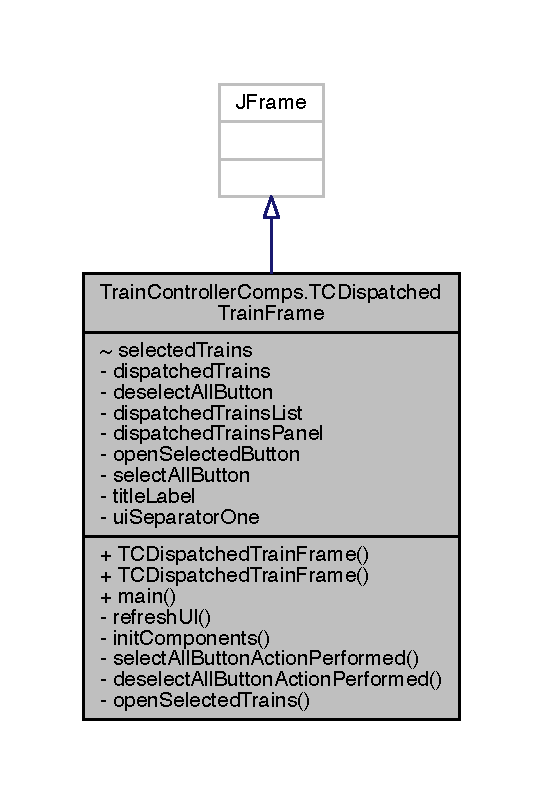
\includegraphics[width=261pt]{classTrainControllerComps_1_1TCDispatchedTrainFrame__inherit__graph}
\end{center}
\end{figure}


Collaboration diagram for Train\+Controller\+Comps.\+T\+C\+Dispatched\+Train\+Frame\+:
\nopagebreak
\begin{figure}[H]
\begin{center}
\leavevmode
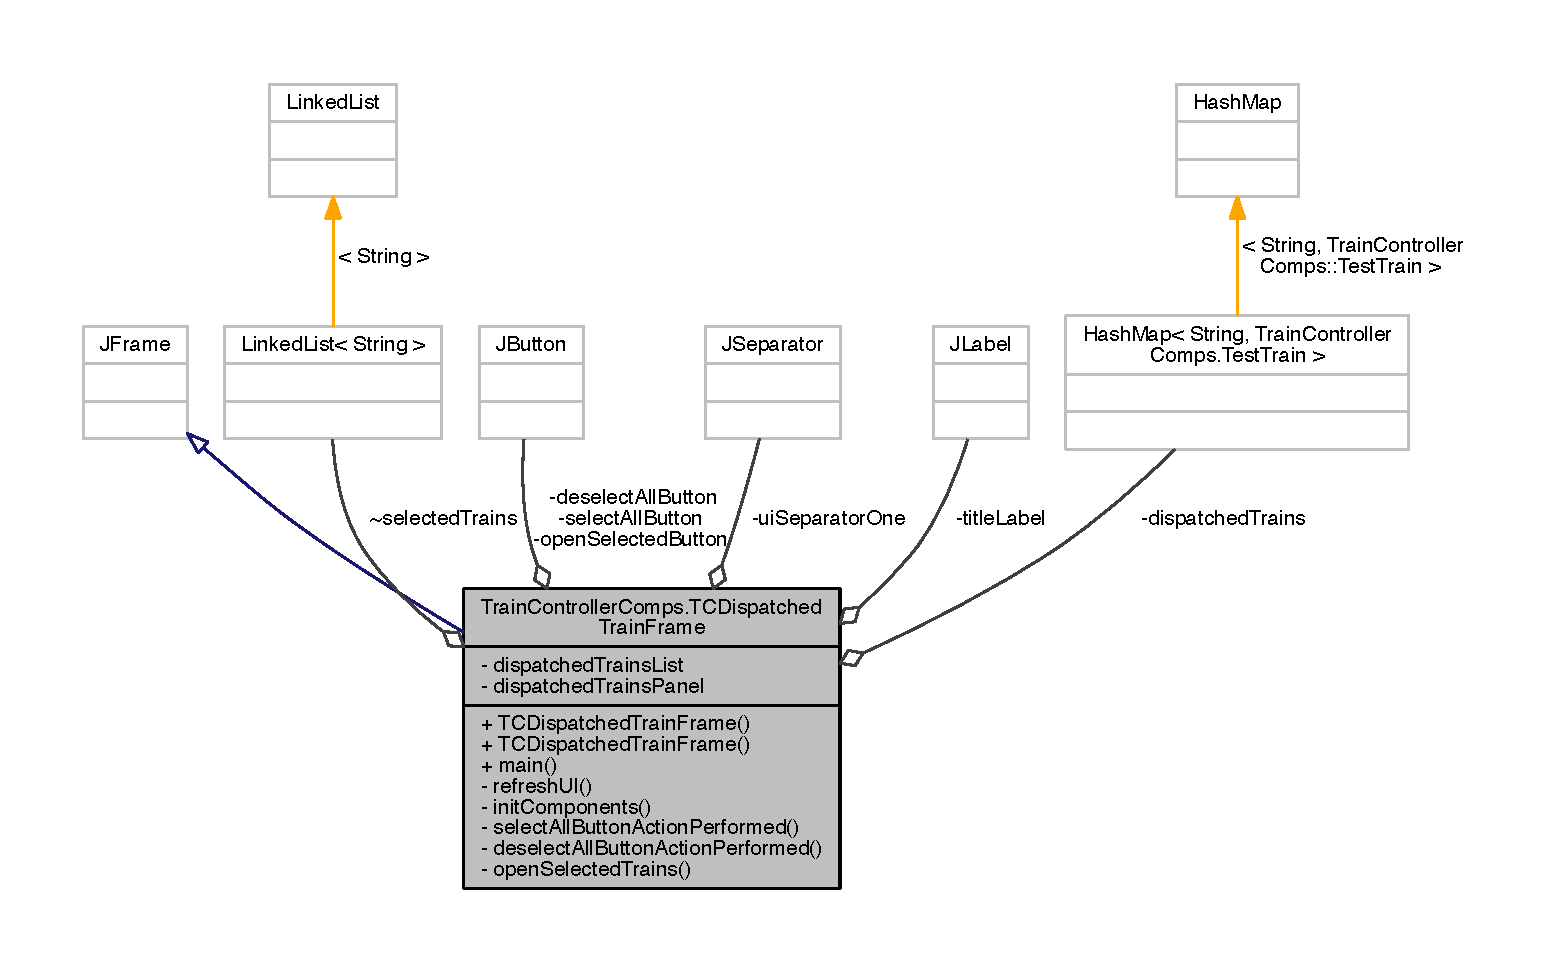
\includegraphics[width=350pt]{classTrainControllerComps_1_1TCDispatchedTrainFrame__coll__graph}
\end{center}
\end{figure}
\subsection*{Public Member Functions}
\begin{DoxyCompactItemize}
\item 
\hyperlink{classTrainControllerComps_1_1TCDispatchedTrainFrame_a4bbebc2384fba3774f4759096804e0b5}{T\+C\+Dispatched\+Train\+Frame} ()
\begin{DoxyCompactList}\small\item\em Constructor for creating a T\+C\+Dispatched\+Frame object. \end{DoxyCompactList}\item 
\hyperlink{classTrainControllerComps_1_1TCDispatchedTrainFrame_af9f9c9d89c8b5f62ed63f59e8514efe9}{T\+C\+Dispatched\+Train\+Frame} (Hash\+Map$<$ String, \hyperlink{classTrainControllerComps_1_1TestTrain}{Test\+Train} $>$ \hyperlink{classTrainControllerComps_1_1TCDispatchedTrainFrame_a4861a7d40d80d413c3eaf3d04b1c1856}{dispatched\+Trains})
\begin{DoxyCompactList}\small\item\em Constructor for creating a T\+C\+Dispatched\+Frame object with a specific Hash\+Map. \end{DoxyCompactList}\end{DoxyCompactItemize}
\subsection*{Static Public Member Functions}
\begin{DoxyCompactItemize}
\item 
static void \hyperlink{classTrainControllerComps_1_1TCDispatchedTrainFrame_aadd36928a24d8836ea28728d6e81ce67}{main} (String args\mbox{[}$\,$\mbox{]})
\end{DoxyCompactItemize}
\subsection*{Package Attributes}
\begin{DoxyCompactItemize}
\item 
Linked\+List$<$ String $>$ \hyperlink{classTrainControllerComps_1_1TCDispatchedTrainFrame_a494919f3599b6980433ef5d370119148}{selected\+Trains}
\begin{DoxyCompactList}\small\item\em A list of trains that the user selected to open a Train Controller for. \end{DoxyCompactList}\end{DoxyCompactItemize}
\subsection*{Private Member Functions}
\begin{DoxyCompactItemize}
\item 
void \hyperlink{classTrainControllerComps_1_1TCDispatchedTrainFrame_aa28b4a0ad4f88726984015206db66ab8}{refresh\+UI} ()
\begin{DoxyCompactList}\small\item\em Refreshes the UI by adding the dispatched trains from the Hash\+Map to the J\+List object embedded in the panel. \end{DoxyCompactList}\item 
void \hyperlink{classTrainControllerComps_1_1TCDispatchedTrainFrame_a7bbb347b25d41c9df04777346a1fd5b6}{init\+Components} ()
\begin{DoxyCompactList}\small\item\em This method is called from within the constructor to initialize the form. \end{DoxyCompactList}\item 
void \hyperlink{classTrainControllerComps_1_1TCDispatchedTrainFrame_a0eb1b68c1e998a0d19cbe6b68fe5576c}{select\+All\+Button\+Action\+Performed} (java.\+awt.\+event.\+Action\+Event evt)
\begin{DoxyCompactList}\small\item\em Selects all the dispatched trains from the dispatched\+Trains\+List. \end{DoxyCompactList}\item 
void \hyperlink{classTrainControllerComps_1_1TCDispatchedTrainFrame_a45691ba29b476f2b2deb616e88dbb498}{deselect\+All\+Button\+Action\+Performed} (java.\+awt.\+event.\+Action\+Event evt)
\begin{DoxyCompactList}\small\item\em Deselects all the trains that are selected in the dispatched\+Trains\+List. \end{DoxyCompactList}\item 
void \hyperlink{classTrainControllerComps_1_1TCDispatchedTrainFrame_a80f4dcaad673ecbc84321b4662ed526a}{open\+Selected\+Trains} (java.\+awt.\+event.\+Action\+Event evt)
\begin{DoxyCompactList}\small\item\em Creates a Train Controller object for each of the trains that were selected by the user. \end{DoxyCompactList}\end{DoxyCompactItemize}
\subsection*{Private Attributes}
\begin{DoxyCompactItemize}
\item 
Hash\+Map$<$ String, \hyperlink{classTrainControllerComps_1_1TestTrain}{Test\+Train} $>$ \hyperlink{classTrainControllerComps_1_1TCDispatchedTrainFrame_a4861a7d40d80d413c3eaf3d04b1c1856}{dispatched\+Trains}
\begin{DoxyCompactList}\small\item\em Hash\+Map used to store the dispatched trains by its unique ID. \end{DoxyCompactList}\item 
javax.\+swing.\+J\+Button \hyperlink{classTrainControllerComps_1_1TCDispatchedTrainFrame_a9af2d015fabe34c39a0d7106ad1f232f}{deselect\+All\+Button}
\item 
javax.\+swing.\+J\+List$<$ String $>$ \hyperlink{classTrainControllerComps_1_1TCDispatchedTrainFrame_a9d75037726700337edcf8650b2acf4e5}{dispatched\+Trains\+List}
\item 
javax.\+swing.\+J\+Scroll\+Pane \hyperlink{classTrainControllerComps_1_1TCDispatchedTrainFrame_a6b12bfbc7c16813288622bb8041547dc}{dispatched\+Trains\+Panel}
\item 
javax.\+swing.\+J\+Button \hyperlink{classTrainControllerComps_1_1TCDispatchedTrainFrame_a4f8d9159144308d5f7471cb7f9c9500b}{open\+Selected\+Button}
\item 
javax.\+swing.\+J\+Button \hyperlink{classTrainControllerComps_1_1TCDispatchedTrainFrame_aa6abdbfd2b8586691278054853911d2f}{select\+All\+Button}
\item 
javax.\+swing.\+J\+Label \hyperlink{classTrainControllerComps_1_1TCDispatchedTrainFrame_aa1201d92fea0fab4d91da28fb35b6f30}{title\+Label}
\item 
javax.\+swing.\+J\+Separator \hyperlink{classTrainControllerComps_1_1TCDispatchedTrainFrame_a42d0aee0b3cc44b2bb9fa31c26228269}{ui\+Separator\+One}
\end{DoxyCompactItemize}


\subsection{Detailed Description}
This class is responsible for displaying all the dispatched trains to the user, and allow them to open multiple Train Controllers for selected trains. 

This class collaborates with the Train Controller class.

\begin{DoxyAuthor}{Author}
Andrew Lendacky 
\end{DoxyAuthor}


\subsection{Constructor \& Destructor Documentation}
\mbox{\Hypertarget{classTrainControllerComps_1_1TCDispatchedTrainFrame_a4bbebc2384fba3774f4759096804e0b5}\label{classTrainControllerComps_1_1TCDispatchedTrainFrame_a4bbebc2384fba3774f4759096804e0b5}} 
\index{Train\+Controller\+Comps\+::\+T\+C\+Dispatched\+Train\+Frame@{Train\+Controller\+Comps\+::\+T\+C\+Dispatched\+Train\+Frame}!T\+C\+Dispatched\+Train\+Frame@{T\+C\+Dispatched\+Train\+Frame}}
\index{T\+C\+Dispatched\+Train\+Frame@{T\+C\+Dispatched\+Train\+Frame}!Train\+Controller\+Comps\+::\+T\+C\+Dispatched\+Train\+Frame@{Train\+Controller\+Comps\+::\+T\+C\+Dispatched\+Train\+Frame}}
\subsubsection{\texorpdfstring{T\+C\+Dispatched\+Train\+Frame()}{TCDispatchedTrainFrame()}\hspace{0.1cm}{\footnotesize\ttfamily [1/2]}}
{\footnotesize\ttfamily Train\+Controller\+Comps.\+T\+C\+Dispatched\+Train\+Frame.\+T\+C\+Dispatched\+Train\+Frame (\begin{DoxyParamCaption}{ }\end{DoxyParamCaption})}



Constructor for creating a T\+C\+Dispatched\+Frame object. 

This constructor does not set the dispatched\+Trains or the selected\+Trains fields. \mbox{\Hypertarget{classTrainControllerComps_1_1TCDispatchedTrainFrame_af9f9c9d89c8b5f62ed63f59e8514efe9}\label{classTrainControllerComps_1_1TCDispatchedTrainFrame_af9f9c9d89c8b5f62ed63f59e8514efe9}} 
\index{Train\+Controller\+Comps\+::\+T\+C\+Dispatched\+Train\+Frame@{Train\+Controller\+Comps\+::\+T\+C\+Dispatched\+Train\+Frame}!T\+C\+Dispatched\+Train\+Frame@{T\+C\+Dispatched\+Train\+Frame}}
\index{T\+C\+Dispatched\+Train\+Frame@{T\+C\+Dispatched\+Train\+Frame}!Train\+Controller\+Comps\+::\+T\+C\+Dispatched\+Train\+Frame@{Train\+Controller\+Comps\+::\+T\+C\+Dispatched\+Train\+Frame}}
\subsubsection{\texorpdfstring{T\+C\+Dispatched\+Train\+Frame()}{TCDispatchedTrainFrame()}\hspace{0.1cm}{\footnotesize\ttfamily [2/2]}}
{\footnotesize\ttfamily Train\+Controller\+Comps.\+T\+C\+Dispatched\+Train\+Frame.\+T\+C\+Dispatched\+Train\+Frame (\begin{DoxyParamCaption}\item[{Hash\+Map$<$ String, \hyperlink{classTrainControllerComps_1_1TestTrain}{Test\+Train} $>$}]{dispatched\+Trains }\end{DoxyParamCaption})}



Constructor for creating a T\+C\+Dispatched\+Frame object with a specific Hash\+Map. 

This Hash\+Map should be passed from the Train Controller class.


\begin{DoxyParams}{Parameters}
{\em dispatched\+Trains} & Hash\+Map corresponding to the dispatched trains. \\
\hline
\end{DoxyParams}


\subsection{Member Function Documentation}
\mbox{\Hypertarget{classTrainControllerComps_1_1TCDispatchedTrainFrame_a45691ba29b476f2b2deb616e88dbb498}\label{classTrainControllerComps_1_1TCDispatchedTrainFrame_a45691ba29b476f2b2deb616e88dbb498}} 
\index{Train\+Controller\+Comps\+::\+T\+C\+Dispatched\+Train\+Frame@{Train\+Controller\+Comps\+::\+T\+C\+Dispatched\+Train\+Frame}!deselect\+All\+Button\+Action\+Performed@{deselect\+All\+Button\+Action\+Performed}}
\index{deselect\+All\+Button\+Action\+Performed@{deselect\+All\+Button\+Action\+Performed}!Train\+Controller\+Comps\+::\+T\+C\+Dispatched\+Train\+Frame@{Train\+Controller\+Comps\+::\+T\+C\+Dispatched\+Train\+Frame}}
\subsubsection{\texorpdfstring{deselect\+All\+Button\+Action\+Performed()}{deselectAllButtonActionPerformed()}}
{\footnotesize\ttfamily void Train\+Controller\+Comps.\+T\+C\+Dispatched\+Train\+Frame.\+deselect\+All\+Button\+Action\+Performed (\begin{DoxyParamCaption}\item[{java.\+awt.\+event.\+Action\+Event}]{evt }\end{DoxyParamCaption})\hspace{0.3cm}{\ttfamily [private]}}



Deselects all the trains that are selected in the dispatched\+Trains\+List. 


\begin{DoxyParams}{Parameters}
{\em evt} & the sender of the event, i.\+e., the \textquotesingle{}Deselect All\textquotesingle{} button \\
\hline
\end{DoxyParams}
\mbox{\Hypertarget{classTrainControllerComps_1_1TCDispatchedTrainFrame_a7bbb347b25d41c9df04777346a1fd5b6}\label{classTrainControllerComps_1_1TCDispatchedTrainFrame_a7bbb347b25d41c9df04777346a1fd5b6}} 
\index{Train\+Controller\+Comps\+::\+T\+C\+Dispatched\+Train\+Frame@{Train\+Controller\+Comps\+::\+T\+C\+Dispatched\+Train\+Frame}!init\+Components@{init\+Components}}
\index{init\+Components@{init\+Components}!Train\+Controller\+Comps\+::\+T\+C\+Dispatched\+Train\+Frame@{Train\+Controller\+Comps\+::\+T\+C\+Dispatched\+Train\+Frame}}
\subsubsection{\texorpdfstring{init\+Components()}{initComponents()}}
{\footnotesize\ttfamily void Train\+Controller\+Comps.\+T\+C\+Dispatched\+Train\+Frame.\+init\+Components (\begin{DoxyParamCaption}{ }\end{DoxyParamCaption})\hspace{0.3cm}{\ttfamily [private]}}



This method is called from within the constructor to initialize the form. 

W\+A\+R\+N\+I\+NG\+: Do N\+OT modify this code. The content of this method is always regenerated by the Form Editor. \mbox{\Hypertarget{classTrainControllerComps_1_1TCDispatchedTrainFrame_aadd36928a24d8836ea28728d6e81ce67}\label{classTrainControllerComps_1_1TCDispatchedTrainFrame_aadd36928a24d8836ea28728d6e81ce67}} 
\index{Train\+Controller\+Comps\+::\+T\+C\+Dispatched\+Train\+Frame@{Train\+Controller\+Comps\+::\+T\+C\+Dispatched\+Train\+Frame}!main@{main}}
\index{main@{main}!Train\+Controller\+Comps\+::\+T\+C\+Dispatched\+Train\+Frame@{Train\+Controller\+Comps\+::\+T\+C\+Dispatched\+Train\+Frame}}
\subsubsection{\texorpdfstring{main()}{main()}}
{\footnotesize\ttfamily static void Train\+Controller\+Comps.\+T\+C\+Dispatched\+Train\+Frame.\+main (\begin{DoxyParamCaption}\item[{String}]{args\mbox{[}$\,$\mbox{]} }\end{DoxyParamCaption})\hspace{0.3cm}{\ttfamily [static]}}


\begin{DoxyParams}{Parameters}
{\em args} & the command line arguments \\
\hline
\end{DoxyParams}
\mbox{\Hypertarget{classTrainControllerComps_1_1TCDispatchedTrainFrame_a80f4dcaad673ecbc84321b4662ed526a}\label{classTrainControllerComps_1_1TCDispatchedTrainFrame_a80f4dcaad673ecbc84321b4662ed526a}} 
\index{Train\+Controller\+Comps\+::\+T\+C\+Dispatched\+Train\+Frame@{Train\+Controller\+Comps\+::\+T\+C\+Dispatched\+Train\+Frame}!open\+Selected\+Trains@{open\+Selected\+Trains}}
\index{open\+Selected\+Trains@{open\+Selected\+Trains}!Train\+Controller\+Comps\+::\+T\+C\+Dispatched\+Train\+Frame@{Train\+Controller\+Comps\+::\+T\+C\+Dispatched\+Train\+Frame}}
\subsubsection{\texorpdfstring{open\+Selected\+Trains()}{openSelectedTrains()}}
{\footnotesize\ttfamily void Train\+Controller\+Comps.\+T\+C\+Dispatched\+Train\+Frame.\+open\+Selected\+Trains (\begin{DoxyParamCaption}\item[{java.\+awt.\+event.\+Action\+Event}]{evt }\end{DoxyParamCaption})\hspace{0.3cm}{\ttfamily [private]}}



Creates a Train Controller object for each of the trains that were selected by the user. 


\begin{DoxyParams}{Parameters}
{\em evt} & the sender of the event, i.\+e., the \textquotesingle{}Open Selected\textquotesingle{} button. \\
\hline
\end{DoxyParams}
\mbox{\Hypertarget{classTrainControllerComps_1_1TCDispatchedTrainFrame_aa28b4a0ad4f88726984015206db66ab8}\label{classTrainControllerComps_1_1TCDispatchedTrainFrame_aa28b4a0ad4f88726984015206db66ab8}} 
\index{Train\+Controller\+Comps\+::\+T\+C\+Dispatched\+Train\+Frame@{Train\+Controller\+Comps\+::\+T\+C\+Dispatched\+Train\+Frame}!refresh\+UI@{refresh\+UI}}
\index{refresh\+UI@{refresh\+UI}!Train\+Controller\+Comps\+::\+T\+C\+Dispatched\+Train\+Frame@{Train\+Controller\+Comps\+::\+T\+C\+Dispatched\+Train\+Frame}}
\subsubsection{\texorpdfstring{refresh\+U\+I()}{refreshUI()}}
{\footnotesize\ttfamily void Train\+Controller\+Comps.\+T\+C\+Dispatched\+Train\+Frame.\+refresh\+UI (\begin{DoxyParamCaption}{ }\end{DoxyParamCaption})\hspace{0.3cm}{\ttfamily [private]}}



Refreshes the UI by adding the dispatched trains from the Hash\+Map to the J\+List object embedded in the panel. 

\mbox{\Hypertarget{classTrainControllerComps_1_1TCDispatchedTrainFrame_a0eb1b68c1e998a0d19cbe6b68fe5576c}\label{classTrainControllerComps_1_1TCDispatchedTrainFrame_a0eb1b68c1e998a0d19cbe6b68fe5576c}} 
\index{Train\+Controller\+Comps\+::\+T\+C\+Dispatched\+Train\+Frame@{Train\+Controller\+Comps\+::\+T\+C\+Dispatched\+Train\+Frame}!select\+All\+Button\+Action\+Performed@{select\+All\+Button\+Action\+Performed}}
\index{select\+All\+Button\+Action\+Performed@{select\+All\+Button\+Action\+Performed}!Train\+Controller\+Comps\+::\+T\+C\+Dispatched\+Train\+Frame@{Train\+Controller\+Comps\+::\+T\+C\+Dispatched\+Train\+Frame}}
\subsubsection{\texorpdfstring{select\+All\+Button\+Action\+Performed()}{selectAllButtonActionPerformed()}}
{\footnotesize\ttfamily void Train\+Controller\+Comps.\+T\+C\+Dispatched\+Train\+Frame.\+select\+All\+Button\+Action\+Performed (\begin{DoxyParamCaption}\item[{java.\+awt.\+event.\+Action\+Event}]{evt }\end{DoxyParamCaption})\hspace{0.3cm}{\ttfamily [private]}}



Selects all the dispatched trains from the dispatched\+Trains\+List. 


\begin{DoxyParams}{Parameters}
{\em evt} & the sender of the event, i.\+e., the \textquotesingle{}Select All\textquotesingle{} button. \\
\hline
\end{DoxyParams}


\subsection{Member Data Documentation}
\mbox{\Hypertarget{classTrainControllerComps_1_1TCDispatchedTrainFrame_a9af2d015fabe34c39a0d7106ad1f232f}\label{classTrainControllerComps_1_1TCDispatchedTrainFrame_a9af2d015fabe34c39a0d7106ad1f232f}} 
\index{Train\+Controller\+Comps\+::\+T\+C\+Dispatched\+Train\+Frame@{Train\+Controller\+Comps\+::\+T\+C\+Dispatched\+Train\+Frame}!deselect\+All\+Button@{deselect\+All\+Button}}
\index{deselect\+All\+Button@{deselect\+All\+Button}!Train\+Controller\+Comps\+::\+T\+C\+Dispatched\+Train\+Frame@{Train\+Controller\+Comps\+::\+T\+C\+Dispatched\+Train\+Frame}}
\subsubsection{\texorpdfstring{deselect\+All\+Button}{deselectAllButton}}
{\footnotesize\ttfamily javax.\+swing.\+J\+Button Train\+Controller\+Comps.\+T\+C\+Dispatched\+Train\+Frame.\+deselect\+All\+Button\hspace{0.3cm}{\ttfamily [private]}}

\mbox{\Hypertarget{classTrainControllerComps_1_1TCDispatchedTrainFrame_a4861a7d40d80d413c3eaf3d04b1c1856}\label{classTrainControllerComps_1_1TCDispatchedTrainFrame_a4861a7d40d80d413c3eaf3d04b1c1856}} 
\index{Train\+Controller\+Comps\+::\+T\+C\+Dispatched\+Train\+Frame@{Train\+Controller\+Comps\+::\+T\+C\+Dispatched\+Train\+Frame}!dispatched\+Trains@{dispatched\+Trains}}
\index{dispatched\+Trains@{dispatched\+Trains}!Train\+Controller\+Comps\+::\+T\+C\+Dispatched\+Train\+Frame@{Train\+Controller\+Comps\+::\+T\+C\+Dispatched\+Train\+Frame}}
\subsubsection{\texorpdfstring{dispatched\+Trains}{dispatchedTrains}}
{\footnotesize\ttfamily Hash\+Map$<$String, \hyperlink{classTrainControllerComps_1_1TestTrain}{Test\+Train}$>$ Train\+Controller\+Comps.\+T\+C\+Dispatched\+Train\+Frame.\+dispatched\+Trains\hspace{0.3cm}{\ttfamily [private]}}



Hash\+Map used to store the dispatched trains by its unique ID. 

\mbox{\Hypertarget{classTrainControllerComps_1_1TCDispatchedTrainFrame_a9d75037726700337edcf8650b2acf4e5}\label{classTrainControllerComps_1_1TCDispatchedTrainFrame_a9d75037726700337edcf8650b2acf4e5}} 
\index{Train\+Controller\+Comps\+::\+T\+C\+Dispatched\+Train\+Frame@{Train\+Controller\+Comps\+::\+T\+C\+Dispatched\+Train\+Frame}!dispatched\+Trains\+List@{dispatched\+Trains\+List}}
\index{dispatched\+Trains\+List@{dispatched\+Trains\+List}!Train\+Controller\+Comps\+::\+T\+C\+Dispatched\+Train\+Frame@{Train\+Controller\+Comps\+::\+T\+C\+Dispatched\+Train\+Frame}}
\subsubsection{\texorpdfstring{dispatched\+Trains\+List}{dispatchedTrainsList}}
{\footnotesize\ttfamily javax.\+swing.\+J\+List$<$String$>$ Train\+Controller\+Comps.\+T\+C\+Dispatched\+Train\+Frame.\+dispatched\+Trains\+List\hspace{0.3cm}{\ttfamily [private]}}

\mbox{\Hypertarget{classTrainControllerComps_1_1TCDispatchedTrainFrame_a6b12bfbc7c16813288622bb8041547dc}\label{classTrainControllerComps_1_1TCDispatchedTrainFrame_a6b12bfbc7c16813288622bb8041547dc}} 
\index{Train\+Controller\+Comps\+::\+T\+C\+Dispatched\+Train\+Frame@{Train\+Controller\+Comps\+::\+T\+C\+Dispatched\+Train\+Frame}!dispatched\+Trains\+Panel@{dispatched\+Trains\+Panel}}
\index{dispatched\+Trains\+Panel@{dispatched\+Trains\+Panel}!Train\+Controller\+Comps\+::\+T\+C\+Dispatched\+Train\+Frame@{Train\+Controller\+Comps\+::\+T\+C\+Dispatched\+Train\+Frame}}
\subsubsection{\texorpdfstring{dispatched\+Trains\+Panel}{dispatchedTrainsPanel}}
{\footnotesize\ttfamily javax.\+swing.\+J\+Scroll\+Pane Train\+Controller\+Comps.\+T\+C\+Dispatched\+Train\+Frame.\+dispatched\+Trains\+Panel\hspace{0.3cm}{\ttfamily [private]}}

\mbox{\Hypertarget{classTrainControllerComps_1_1TCDispatchedTrainFrame_a4f8d9159144308d5f7471cb7f9c9500b}\label{classTrainControllerComps_1_1TCDispatchedTrainFrame_a4f8d9159144308d5f7471cb7f9c9500b}} 
\index{Train\+Controller\+Comps\+::\+T\+C\+Dispatched\+Train\+Frame@{Train\+Controller\+Comps\+::\+T\+C\+Dispatched\+Train\+Frame}!open\+Selected\+Button@{open\+Selected\+Button}}
\index{open\+Selected\+Button@{open\+Selected\+Button}!Train\+Controller\+Comps\+::\+T\+C\+Dispatched\+Train\+Frame@{Train\+Controller\+Comps\+::\+T\+C\+Dispatched\+Train\+Frame}}
\subsubsection{\texorpdfstring{open\+Selected\+Button}{openSelectedButton}}
{\footnotesize\ttfamily javax.\+swing.\+J\+Button Train\+Controller\+Comps.\+T\+C\+Dispatched\+Train\+Frame.\+open\+Selected\+Button\hspace{0.3cm}{\ttfamily [private]}}

\mbox{\Hypertarget{classTrainControllerComps_1_1TCDispatchedTrainFrame_aa6abdbfd2b8586691278054853911d2f}\label{classTrainControllerComps_1_1TCDispatchedTrainFrame_aa6abdbfd2b8586691278054853911d2f}} 
\index{Train\+Controller\+Comps\+::\+T\+C\+Dispatched\+Train\+Frame@{Train\+Controller\+Comps\+::\+T\+C\+Dispatched\+Train\+Frame}!select\+All\+Button@{select\+All\+Button}}
\index{select\+All\+Button@{select\+All\+Button}!Train\+Controller\+Comps\+::\+T\+C\+Dispatched\+Train\+Frame@{Train\+Controller\+Comps\+::\+T\+C\+Dispatched\+Train\+Frame}}
\subsubsection{\texorpdfstring{select\+All\+Button}{selectAllButton}}
{\footnotesize\ttfamily javax.\+swing.\+J\+Button Train\+Controller\+Comps.\+T\+C\+Dispatched\+Train\+Frame.\+select\+All\+Button\hspace{0.3cm}{\ttfamily [private]}}

\mbox{\Hypertarget{classTrainControllerComps_1_1TCDispatchedTrainFrame_a494919f3599b6980433ef5d370119148}\label{classTrainControllerComps_1_1TCDispatchedTrainFrame_a494919f3599b6980433ef5d370119148}} 
\index{Train\+Controller\+Comps\+::\+T\+C\+Dispatched\+Train\+Frame@{Train\+Controller\+Comps\+::\+T\+C\+Dispatched\+Train\+Frame}!selected\+Trains@{selected\+Trains}}
\index{selected\+Trains@{selected\+Trains}!Train\+Controller\+Comps\+::\+T\+C\+Dispatched\+Train\+Frame@{Train\+Controller\+Comps\+::\+T\+C\+Dispatched\+Train\+Frame}}
\subsubsection{\texorpdfstring{selected\+Trains}{selectedTrains}}
{\footnotesize\ttfamily Linked\+List$<$String$>$ Train\+Controller\+Comps.\+T\+C\+Dispatched\+Train\+Frame.\+selected\+Trains\hspace{0.3cm}{\ttfamily [package]}}



A list of trains that the user selected to open a Train Controller for. 

\mbox{\Hypertarget{classTrainControllerComps_1_1TCDispatchedTrainFrame_aa1201d92fea0fab4d91da28fb35b6f30}\label{classTrainControllerComps_1_1TCDispatchedTrainFrame_aa1201d92fea0fab4d91da28fb35b6f30}} 
\index{Train\+Controller\+Comps\+::\+T\+C\+Dispatched\+Train\+Frame@{Train\+Controller\+Comps\+::\+T\+C\+Dispatched\+Train\+Frame}!title\+Label@{title\+Label}}
\index{title\+Label@{title\+Label}!Train\+Controller\+Comps\+::\+T\+C\+Dispatched\+Train\+Frame@{Train\+Controller\+Comps\+::\+T\+C\+Dispatched\+Train\+Frame}}
\subsubsection{\texorpdfstring{title\+Label}{titleLabel}}
{\footnotesize\ttfamily javax.\+swing.\+J\+Label Train\+Controller\+Comps.\+T\+C\+Dispatched\+Train\+Frame.\+title\+Label\hspace{0.3cm}{\ttfamily [private]}}

\mbox{\Hypertarget{classTrainControllerComps_1_1TCDispatchedTrainFrame_a42d0aee0b3cc44b2bb9fa31c26228269}\label{classTrainControllerComps_1_1TCDispatchedTrainFrame_a42d0aee0b3cc44b2bb9fa31c26228269}} 
\index{Train\+Controller\+Comps\+::\+T\+C\+Dispatched\+Train\+Frame@{Train\+Controller\+Comps\+::\+T\+C\+Dispatched\+Train\+Frame}!ui\+Separator\+One@{ui\+Separator\+One}}
\index{ui\+Separator\+One@{ui\+Separator\+One}!Train\+Controller\+Comps\+::\+T\+C\+Dispatched\+Train\+Frame@{Train\+Controller\+Comps\+::\+T\+C\+Dispatched\+Train\+Frame}}
\subsubsection{\texorpdfstring{ui\+Separator\+One}{uiSeparatorOne}}
{\footnotesize\ttfamily javax.\+swing.\+J\+Separator Train\+Controller\+Comps.\+T\+C\+Dispatched\+Train\+Frame.\+ui\+Separator\+One\hspace{0.3cm}{\ttfamily [private]}}



The documentation for this class was generated from the following file\+:\begin{DoxyCompactItemize}
\item 
src/main/java/\+Train\+Controller\+Comps/\hyperlink{TCDispatchedTrainFrame_8java}{T\+C\+Dispatched\+Train\+Frame.\+java}\end{DoxyCompactItemize}

\hypertarget{classTrainControllerComps_1_1TCEmergencyFrame}{}\section{Train\+Controller\+Comps.\+T\+C\+Emergency\+Frame Class Reference}
\label{classTrainControllerComps_1_1TCEmergencyFrame}\index{Train\+Controller\+Comps.\+T\+C\+Emergency\+Frame@{Train\+Controller\+Comps.\+T\+C\+Emergency\+Frame}}


This class is responsible for confirming the use of the selected trains emergency brake when in Manual mode.  




Inheritance diagram for Train\+Controller\+Comps.\+T\+C\+Emergency\+Frame\+:
\nopagebreak
\begin{figure}[H]
\begin{center}
\leavevmode
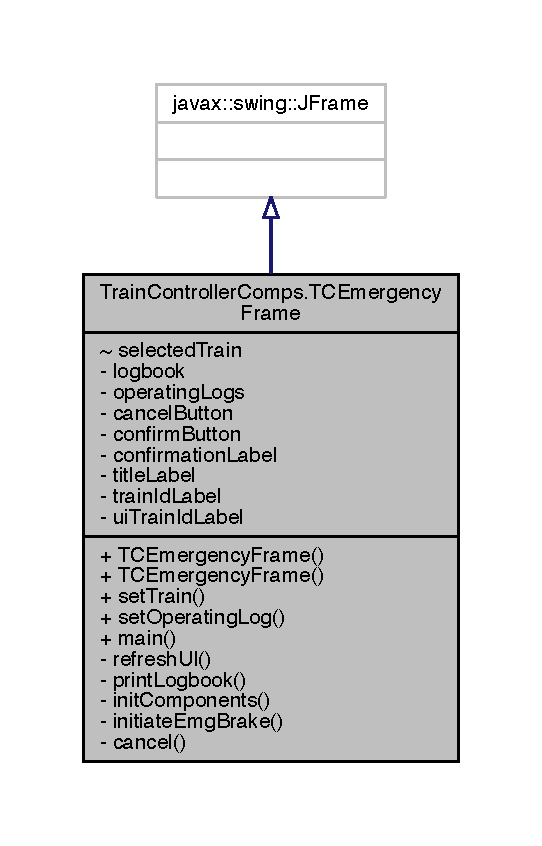
\includegraphics[width=260pt]{classTrainControllerComps_1_1TCEmergencyFrame__inherit__graph}
\end{center}
\end{figure}


Collaboration diagram for Train\+Controller\+Comps.\+T\+C\+Emergency\+Frame\+:
\nopagebreak
\begin{figure}[H]
\begin{center}
\leavevmode
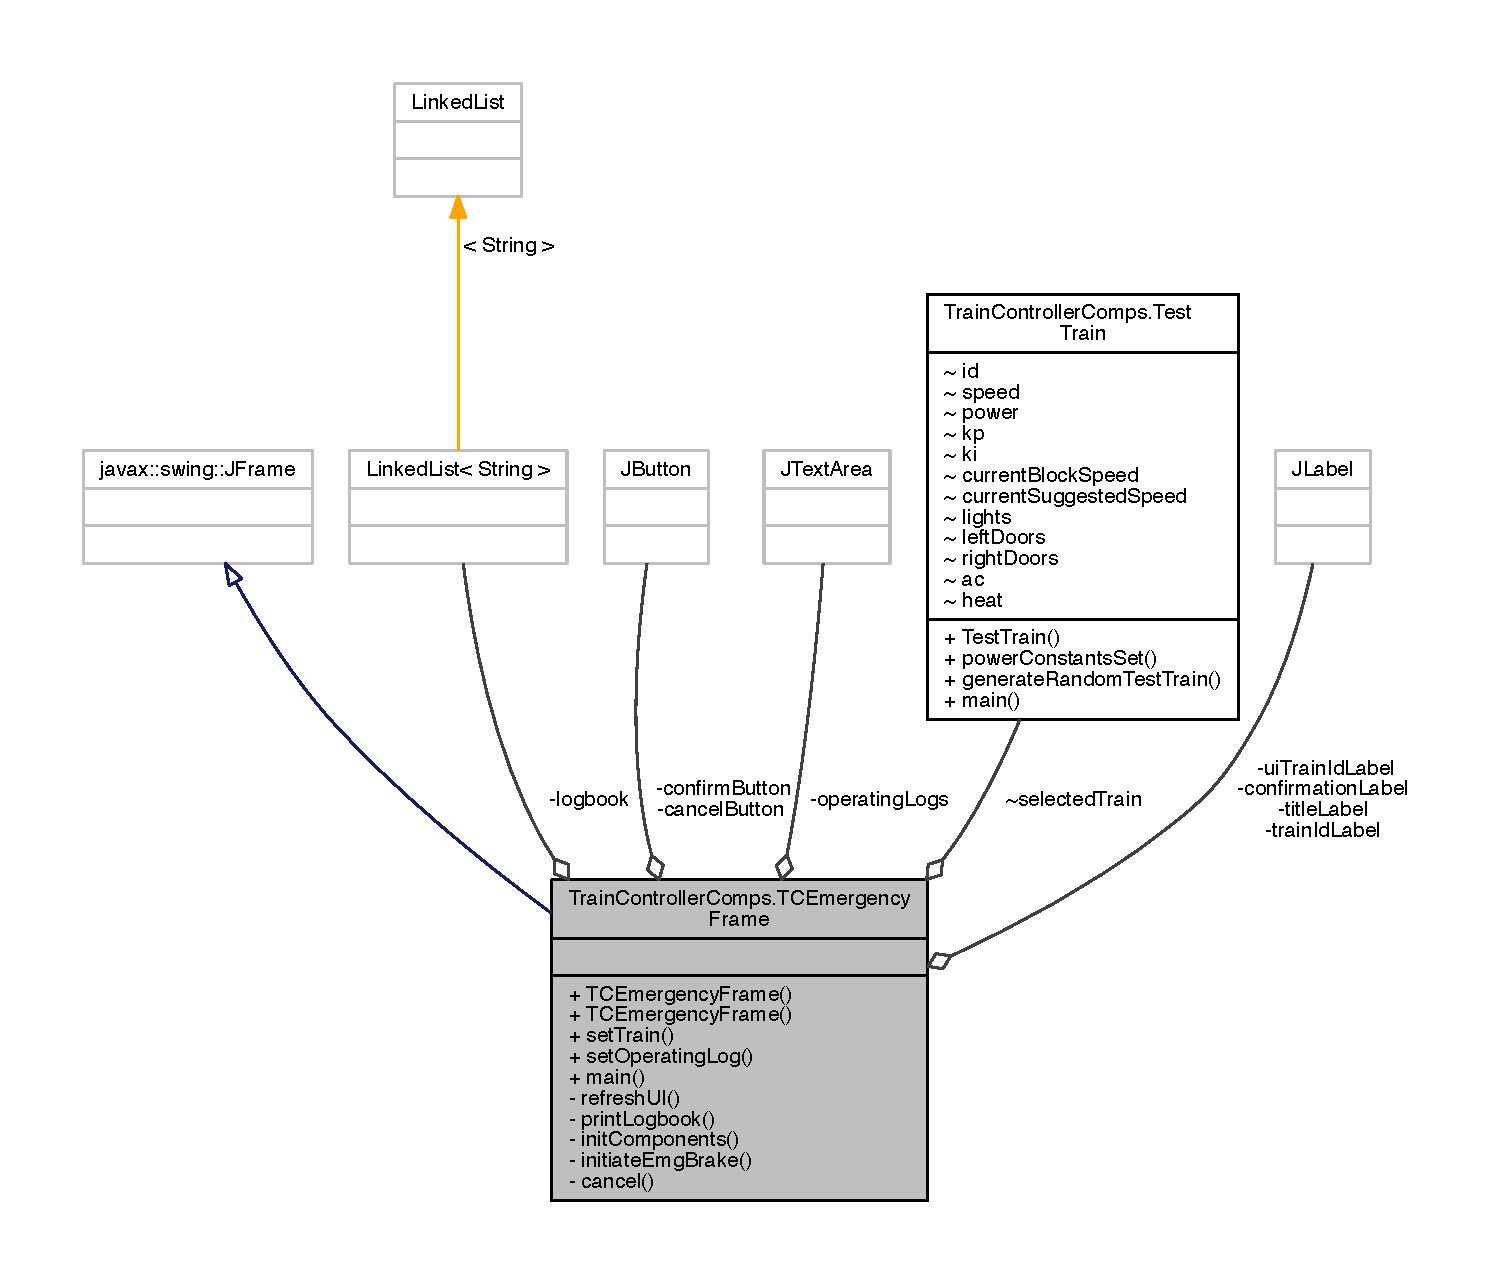
\includegraphics[width=350pt]{classTrainControllerComps_1_1TCEmergencyFrame__coll__graph}
\end{center}
\end{figure}
\subsection*{Public Member Functions}
\begin{DoxyCompactItemize}
\item 
\hyperlink{classTrainControllerComps_1_1TCEmergencyFrame_a318efda39f1845bdcc8beacab2f15f02}{T\+C\+Emergency\+Frame} ()
\begin{DoxyCompactList}\small\item\em Constructor for creating a \hyperlink{classTrainControllerComps_1_1TCEmergencyFrame}{T\+C\+Emergency\+Frame} object without any selected train. \end{DoxyCompactList}\item 
\hyperlink{classTrainControllerComps_1_1TCEmergencyFrame_a389f462d159a3b37df539384297e4aca}{T\+C\+Emergency\+Frame} (\hyperlink{classTrainControllerComps_1_1TestTrain}{Test\+Train} \hyperlink{classtrain}{train})
\begin{DoxyCompactList}\small\item\em Constructor for creating a \hyperlink{classTrainControllerComps_1_1TCEmergencyFrame}{T\+C\+Emergency\+Frame} object with a selected train. \end{DoxyCompactList}\item 
void \hyperlink{classTrainControllerComps_1_1TCEmergencyFrame_a61d8cb274f6be974634700dd6eee045c}{set\+Train} (\hyperlink{classTrainControllerComps_1_1TestTrain}{Test\+Train} \hyperlink{classtrain}{train})
\begin{DoxyCompactList}\small\item\em Sets the selected train. \end{DoxyCompactList}\item 
void \hyperlink{classTrainControllerComps_1_1TCEmergencyFrame_a976ebb5248e43db7b076148f1d1e8f0b}{set\+Operating\+Log} (J\+Text\+Area operating\+Log)
\begin{DoxyCompactList}\small\item\em Sets the operating log to be used to print messages in. \end{DoxyCompactList}\end{DoxyCompactItemize}
\subsection*{Static Public Member Functions}
\begin{DoxyCompactItemize}
\item 
static void \hyperlink{classTrainControllerComps_1_1TCEmergencyFrame_a3a4826e73daed7e795104224492dfd78}{main} (String args\mbox{[}$\,$\mbox{]})
\end{DoxyCompactItemize}
\subsection*{Package Attributes}
\begin{DoxyCompactItemize}
\item 
\hyperlink{classTrainControllerComps_1_1TestTrain}{Test\+Train} \hyperlink{classTrainControllerComps_1_1TCEmergencyFrame_ac99b85a0ae38a4b60920f7ab057eb3c5}{selected\+Train}
\begin{DoxyCompactList}\small\item\em The train that is being controlled by the Train Controller class. \end{DoxyCompactList}\end{DoxyCompactItemize}
\subsection*{Private Member Functions}
\begin{DoxyCompactItemize}
\item 
void \hyperlink{classTrainControllerComps_1_1TCEmergencyFrame_a9314711626f90cd94306caa329311d60}{refresh\+UI} ()
\begin{DoxyCompactList}\small\item\em Refreshes the UI elements in the window to update any changed train information. \end{DoxyCompactList}\item 
void \hyperlink{classTrainControllerComps_1_1TCEmergencyFrame_a6a8c92fdc073a69ed2e86373e145d34a}{print\+Logbook} ()
\begin{DoxyCompactList}\small\item\em Prints the logbook to the operating log, and then clears the logbook. \end{DoxyCompactList}\item 
void \hyperlink{classTrainControllerComps_1_1TCEmergencyFrame_aa5cf83696387c257f09ff198718eaf33}{init\+Components} ()
\begin{DoxyCompactList}\small\item\em This method is called from within the constructor to initialize the form. \end{DoxyCompactList}\item 
void \hyperlink{classTrainControllerComps_1_1TCEmergencyFrame_a03d0a51aadee6e85a856d7f4e1d41677}{initiate\+Emg\+Brake} (java.\+awt.\+event.\+Action\+Event evt)
\begin{DoxyCompactList}\small\item\em Initiates the emergency brake on the selected train. \end{DoxyCompactList}\item 
void \hyperlink{classTrainControllerComps_1_1TCEmergencyFrame_a657c1dcd129d412134610a08c8d3cdfd}{cancel} (java.\+awt.\+event.\+Action\+Event evt)
\begin{DoxyCompactList}\small\item\em Closes the window without engaging the selected train\textquotesingle{}s emergency brake. \end{DoxyCompactList}\end{DoxyCompactItemize}
\subsection*{Private Attributes}
\begin{DoxyCompactItemize}
\item 
Linked\+List$<$ String $>$ \hyperlink{classTrainControllerComps_1_1TCEmergencyFrame_a862e94d85954c294ac65c7ad438e81a1}{logbook}
\begin{DoxyCompactList}\small\item\em List that contains messages that are to be printed to the operating log. \end{DoxyCompactList}\item 
J\+Text\+Area \hyperlink{classTrainControllerComps_1_1TCEmergencyFrame_acc095e29e87ce6e8cb31fbc942303d78}{operating\+Logs}
\begin{DoxyCompactList}\small\item\em Area used to print messaged from the logbook to. \end{DoxyCompactList}\item 
javax.\+swing.\+J\+Button \hyperlink{classTrainControllerComps_1_1TCEmergencyFrame_a26994214c39f2a3b8f0dba373cfb0b5e}{cancel\+Button}
\item 
javax.\+swing.\+J\+Button \hyperlink{classTrainControllerComps_1_1TCEmergencyFrame_a09a53fb532f9214e271fc811c729a274}{confirm\+Button}
\item 
javax.\+swing.\+J\+Label \hyperlink{classTrainControllerComps_1_1TCEmergencyFrame_ab69b8c59e98e915d38dd2eff13711fea}{confirmation\+Label}
\item 
javax.\+swing.\+J\+Label \hyperlink{classTrainControllerComps_1_1TCEmergencyFrame_a611138a25d7b488a12107dc7e3b9efaa}{title\+Label}
\item 
javax.\+swing.\+J\+Label \hyperlink{classTrainControllerComps_1_1TCEmergencyFrame_abcbe7bf869507518346fef39f3701ec7}{train\+Id\+Label}
\item 
javax.\+swing.\+J\+Label \hyperlink{classTrainControllerComps_1_1TCEmergencyFrame_aed0a549c9bb0b9a7adf7b4d81fd21904}{ui\+Train\+Id\+Label}
\end{DoxyCompactItemize}


\subsection{Detailed Description}
This class is responsible for confirming the use of the selected trains emergency brake when in Manual mode. 

This class collaborates with the Train Controller, and the Train class.

\begin{DoxyAuthor}{Author}
Andrew Lendacky 
\end{DoxyAuthor}


\subsection{Constructor \& Destructor Documentation}
\mbox{\Hypertarget{classTrainControllerComps_1_1TCEmergencyFrame_a318efda39f1845bdcc8beacab2f15f02}\label{classTrainControllerComps_1_1TCEmergencyFrame_a318efda39f1845bdcc8beacab2f15f02}} 
\index{Train\+Controller\+Comps\+::\+T\+C\+Emergency\+Frame@{Train\+Controller\+Comps\+::\+T\+C\+Emergency\+Frame}!T\+C\+Emergency\+Frame@{T\+C\+Emergency\+Frame}}
\index{T\+C\+Emergency\+Frame@{T\+C\+Emergency\+Frame}!Train\+Controller\+Comps\+::\+T\+C\+Emergency\+Frame@{Train\+Controller\+Comps\+::\+T\+C\+Emergency\+Frame}}
\subsubsection{\texorpdfstring{T\+C\+Emergency\+Frame()}{TCEmergencyFrame()}\hspace{0.1cm}{\footnotesize\ttfamily [1/2]}}
{\footnotesize\ttfamily Train\+Controller\+Comps.\+T\+C\+Emergency\+Frame.\+T\+C\+Emergency\+Frame (\begin{DoxyParamCaption}{ }\end{DoxyParamCaption})}



Constructor for creating a \hyperlink{classTrainControllerComps_1_1TCEmergencyFrame}{T\+C\+Emergency\+Frame} object without any selected train. 

Selected train must be passed in by the Train Controller class. \mbox{\Hypertarget{classTrainControllerComps_1_1TCEmergencyFrame_a389f462d159a3b37df539384297e4aca}\label{classTrainControllerComps_1_1TCEmergencyFrame_a389f462d159a3b37df539384297e4aca}} 
\index{Train\+Controller\+Comps\+::\+T\+C\+Emergency\+Frame@{Train\+Controller\+Comps\+::\+T\+C\+Emergency\+Frame}!T\+C\+Emergency\+Frame@{T\+C\+Emergency\+Frame}}
\index{T\+C\+Emergency\+Frame@{T\+C\+Emergency\+Frame}!Train\+Controller\+Comps\+::\+T\+C\+Emergency\+Frame@{Train\+Controller\+Comps\+::\+T\+C\+Emergency\+Frame}}
\subsubsection{\texorpdfstring{T\+C\+Emergency\+Frame()}{TCEmergencyFrame()}\hspace{0.1cm}{\footnotesize\ttfamily [2/2]}}
{\footnotesize\ttfamily Train\+Controller\+Comps.\+T\+C\+Emergency\+Frame.\+T\+C\+Emergency\+Frame (\begin{DoxyParamCaption}\item[{\hyperlink{classTrainControllerComps_1_1TestTrain}{Test\+Train}}]{train }\end{DoxyParamCaption})}



Constructor for creating a \hyperlink{classTrainControllerComps_1_1TCEmergencyFrame}{T\+C\+Emergency\+Frame} object with a selected train. 


\begin{DoxyParams}{Parameters}
{\em train} & the train being controlled by the Train Controller \\
\hline
\end{DoxyParams}


\subsection{Member Function Documentation}
\mbox{\Hypertarget{classTrainControllerComps_1_1TCEmergencyFrame_a657c1dcd129d412134610a08c8d3cdfd}\label{classTrainControllerComps_1_1TCEmergencyFrame_a657c1dcd129d412134610a08c8d3cdfd}} 
\index{Train\+Controller\+Comps\+::\+T\+C\+Emergency\+Frame@{Train\+Controller\+Comps\+::\+T\+C\+Emergency\+Frame}!cancel@{cancel}}
\index{cancel@{cancel}!Train\+Controller\+Comps\+::\+T\+C\+Emergency\+Frame@{Train\+Controller\+Comps\+::\+T\+C\+Emergency\+Frame}}
\subsubsection{\texorpdfstring{cancel()}{cancel()}}
{\footnotesize\ttfamily void Train\+Controller\+Comps.\+T\+C\+Emergency\+Frame.\+cancel (\begin{DoxyParamCaption}\item[{java.\+awt.\+event.\+Action\+Event}]{evt }\end{DoxyParamCaption})\hspace{0.3cm}{\ttfamily [private]}}



Closes the window without engaging the selected train\textquotesingle{}s emergency brake. 


\begin{DoxyParams}{Parameters}
{\em evt} & the sender of the event, i.\+e., the \textquotesingle{}Cancel\textquotesingle{} button \\
\hline
\end{DoxyParams}
\mbox{\Hypertarget{classTrainControllerComps_1_1TCEmergencyFrame_aa5cf83696387c257f09ff198718eaf33}\label{classTrainControllerComps_1_1TCEmergencyFrame_aa5cf83696387c257f09ff198718eaf33}} 
\index{Train\+Controller\+Comps\+::\+T\+C\+Emergency\+Frame@{Train\+Controller\+Comps\+::\+T\+C\+Emergency\+Frame}!init\+Components@{init\+Components}}
\index{init\+Components@{init\+Components}!Train\+Controller\+Comps\+::\+T\+C\+Emergency\+Frame@{Train\+Controller\+Comps\+::\+T\+C\+Emergency\+Frame}}
\subsubsection{\texorpdfstring{init\+Components()}{initComponents()}}
{\footnotesize\ttfamily void Train\+Controller\+Comps.\+T\+C\+Emergency\+Frame.\+init\+Components (\begin{DoxyParamCaption}{ }\end{DoxyParamCaption})\hspace{0.3cm}{\ttfamily [private]}}



This method is called from within the constructor to initialize the form. 

W\+A\+R\+N\+I\+NG\+: Do N\+OT modify this code. The content of this method is always regenerated by the Form Editor. \mbox{\Hypertarget{classTrainControllerComps_1_1TCEmergencyFrame_a03d0a51aadee6e85a856d7f4e1d41677}\label{classTrainControllerComps_1_1TCEmergencyFrame_a03d0a51aadee6e85a856d7f4e1d41677}} 
\index{Train\+Controller\+Comps\+::\+T\+C\+Emergency\+Frame@{Train\+Controller\+Comps\+::\+T\+C\+Emergency\+Frame}!initiate\+Emg\+Brake@{initiate\+Emg\+Brake}}
\index{initiate\+Emg\+Brake@{initiate\+Emg\+Brake}!Train\+Controller\+Comps\+::\+T\+C\+Emergency\+Frame@{Train\+Controller\+Comps\+::\+T\+C\+Emergency\+Frame}}
\subsubsection{\texorpdfstring{initiate\+Emg\+Brake()}{initiateEmgBrake()}}
{\footnotesize\ttfamily void Train\+Controller\+Comps.\+T\+C\+Emergency\+Frame.\+initiate\+Emg\+Brake (\begin{DoxyParamCaption}\item[{java.\+awt.\+event.\+Action\+Event}]{evt }\end{DoxyParamCaption})\hspace{0.3cm}{\ttfamily [private]}}



Initiates the emergency brake on the selected train. 


\begin{DoxyParams}{Parameters}
{\em evt} & the sender of the event, i.\+e., the \textquotesingle{}Confirm\textquotesingle{} button \\
\hline
\end{DoxyParams}
\mbox{\Hypertarget{classTrainControllerComps_1_1TCEmergencyFrame_a3a4826e73daed7e795104224492dfd78}\label{classTrainControllerComps_1_1TCEmergencyFrame_a3a4826e73daed7e795104224492dfd78}} 
\index{Train\+Controller\+Comps\+::\+T\+C\+Emergency\+Frame@{Train\+Controller\+Comps\+::\+T\+C\+Emergency\+Frame}!main@{main}}
\index{main@{main}!Train\+Controller\+Comps\+::\+T\+C\+Emergency\+Frame@{Train\+Controller\+Comps\+::\+T\+C\+Emergency\+Frame}}
\subsubsection{\texorpdfstring{main()}{main()}}
{\footnotesize\ttfamily static void Train\+Controller\+Comps.\+T\+C\+Emergency\+Frame.\+main (\begin{DoxyParamCaption}\item[{String}]{args\mbox{[}$\,$\mbox{]} }\end{DoxyParamCaption})\hspace{0.3cm}{\ttfamily [static]}}


\begin{DoxyParams}{Parameters}
{\em args} & the command line arguments \\
\hline
\end{DoxyParams}
\mbox{\Hypertarget{classTrainControllerComps_1_1TCEmergencyFrame_a6a8c92fdc073a69ed2e86373e145d34a}\label{classTrainControllerComps_1_1TCEmergencyFrame_a6a8c92fdc073a69ed2e86373e145d34a}} 
\index{Train\+Controller\+Comps\+::\+T\+C\+Emergency\+Frame@{Train\+Controller\+Comps\+::\+T\+C\+Emergency\+Frame}!print\+Logbook@{print\+Logbook}}
\index{print\+Logbook@{print\+Logbook}!Train\+Controller\+Comps\+::\+T\+C\+Emergency\+Frame@{Train\+Controller\+Comps\+::\+T\+C\+Emergency\+Frame}}
\subsubsection{\texorpdfstring{print\+Logbook()}{printLogbook()}}
{\footnotesize\ttfamily void Train\+Controller\+Comps.\+T\+C\+Emergency\+Frame.\+print\+Logbook (\begin{DoxyParamCaption}{ }\end{DoxyParamCaption})\hspace{0.3cm}{\ttfamily [private]}}



Prints the logbook to the operating log, and then clears the logbook. 

\mbox{\Hypertarget{classTrainControllerComps_1_1TCEmergencyFrame_a9314711626f90cd94306caa329311d60}\label{classTrainControllerComps_1_1TCEmergencyFrame_a9314711626f90cd94306caa329311d60}} 
\index{Train\+Controller\+Comps\+::\+T\+C\+Emergency\+Frame@{Train\+Controller\+Comps\+::\+T\+C\+Emergency\+Frame}!refresh\+UI@{refresh\+UI}}
\index{refresh\+UI@{refresh\+UI}!Train\+Controller\+Comps\+::\+T\+C\+Emergency\+Frame@{Train\+Controller\+Comps\+::\+T\+C\+Emergency\+Frame}}
\subsubsection{\texorpdfstring{refresh\+U\+I()}{refreshUI()}}
{\footnotesize\ttfamily void Train\+Controller\+Comps.\+T\+C\+Emergency\+Frame.\+refresh\+UI (\begin{DoxyParamCaption}{ }\end{DoxyParamCaption})\hspace{0.3cm}{\ttfamily [private]}}



Refreshes the UI elements in the window to update any changed train information. 

\mbox{\Hypertarget{classTrainControllerComps_1_1TCEmergencyFrame_a976ebb5248e43db7b076148f1d1e8f0b}\label{classTrainControllerComps_1_1TCEmergencyFrame_a976ebb5248e43db7b076148f1d1e8f0b}} 
\index{Train\+Controller\+Comps\+::\+T\+C\+Emergency\+Frame@{Train\+Controller\+Comps\+::\+T\+C\+Emergency\+Frame}!set\+Operating\+Log@{set\+Operating\+Log}}
\index{set\+Operating\+Log@{set\+Operating\+Log}!Train\+Controller\+Comps\+::\+T\+C\+Emergency\+Frame@{Train\+Controller\+Comps\+::\+T\+C\+Emergency\+Frame}}
\subsubsection{\texorpdfstring{set\+Operating\+Log()}{setOperatingLog()}}
{\footnotesize\ttfamily void Train\+Controller\+Comps.\+T\+C\+Emergency\+Frame.\+set\+Operating\+Log (\begin{DoxyParamCaption}\item[{J\+Text\+Area}]{operating\+Log }\end{DoxyParamCaption})}



Sets the operating log to be used to print messages in. 


\begin{DoxyParams}{Parameters}
{\em operating\+Log} & the operating log. \\
\hline
\end{DoxyParams}
\mbox{\Hypertarget{classTrainControllerComps_1_1TCEmergencyFrame_a61d8cb274f6be974634700dd6eee045c}\label{classTrainControllerComps_1_1TCEmergencyFrame_a61d8cb274f6be974634700dd6eee045c}} 
\index{Train\+Controller\+Comps\+::\+T\+C\+Emergency\+Frame@{Train\+Controller\+Comps\+::\+T\+C\+Emergency\+Frame}!set\+Train@{set\+Train}}
\index{set\+Train@{set\+Train}!Train\+Controller\+Comps\+::\+T\+C\+Emergency\+Frame@{Train\+Controller\+Comps\+::\+T\+C\+Emergency\+Frame}}
\subsubsection{\texorpdfstring{set\+Train()}{setTrain()}}
{\footnotesize\ttfamily void Train\+Controller\+Comps.\+T\+C\+Emergency\+Frame.\+set\+Train (\begin{DoxyParamCaption}\item[{\hyperlink{classTrainControllerComps_1_1TestTrain}{Test\+Train}}]{train }\end{DoxyParamCaption})}



Sets the selected train. 

This method should be called from the Train Controller class.


\begin{DoxyParams}{Parameters}
{\em train} & the selected train controlled by the Train Controller class. \\
\hline
\end{DoxyParams}


\subsection{Member Data Documentation}
\mbox{\Hypertarget{classTrainControllerComps_1_1TCEmergencyFrame_a26994214c39f2a3b8f0dba373cfb0b5e}\label{classTrainControllerComps_1_1TCEmergencyFrame_a26994214c39f2a3b8f0dba373cfb0b5e}} 
\index{Train\+Controller\+Comps\+::\+T\+C\+Emergency\+Frame@{Train\+Controller\+Comps\+::\+T\+C\+Emergency\+Frame}!cancel\+Button@{cancel\+Button}}
\index{cancel\+Button@{cancel\+Button}!Train\+Controller\+Comps\+::\+T\+C\+Emergency\+Frame@{Train\+Controller\+Comps\+::\+T\+C\+Emergency\+Frame}}
\subsubsection{\texorpdfstring{cancel\+Button}{cancelButton}}
{\footnotesize\ttfamily javax.\+swing.\+J\+Button Train\+Controller\+Comps.\+T\+C\+Emergency\+Frame.\+cancel\+Button\hspace{0.3cm}{\ttfamily [private]}}

\mbox{\Hypertarget{classTrainControllerComps_1_1TCEmergencyFrame_ab69b8c59e98e915d38dd2eff13711fea}\label{classTrainControllerComps_1_1TCEmergencyFrame_ab69b8c59e98e915d38dd2eff13711fea}} 
\index{Train\+Controller\+Comps\+::\+T\+C\+Emergency\+Frame@{Train\+Controller\+Comps\+::\+T\+C\+Emergency\+Frame}!confirmation\+Label@{confirmation\+Label}}
\index{confirmation\+Label@{confirmation\+Label}!Train\+Controller\+Comps\+::\+T\+C\+Emergency\+Frame@{Train\+Controller\+Comps\+::\+T\+C\+Emergency\+Frame}}
\subsubsection{\texorpdfstring{confirmation\+Label}{confirmationLabel}}
{\footnotesize\ttfamily javax.\+swing.\+J\+Label Train\+Controller\+Comps.\+T\+C\+Emergency\+Frame.\+confirmation\+Label\hspace{0.3cm}{\ttfamily [private]}}

\mbox{\Hypertarget{classTrainControllerComps_1_1TCEmergencyFrame_a09a53fb532f9214e271fc811c729a274}\label{classTrainControllerComps_1_1TCEmergencyFrame_a09a53fb532f9214e271fc811c729a274}} 
\index{Train\+Controller\+Comps\+::\+T\+C\+Emergency\+Frame@{Train\+Controller\+Comps\+::\+T\+C\+Emergency\+Frame}!confirm\+Button@{confirm\+Button}}
\index{confirm\+Button@{confirm\+Button}!Train\+Controller\+Comps\+::\+T\+C\+Emergency\+Frame@{Train\+Controller\+Comps\+::\+T\+C\+Emergency\+Frame}}
\subsubsection{\texorpdfstring{confirm\+Button}{confirmButton}}
{\footnotesize\ttfamily javax.\+swing.\+J\+Button Train\+Controller\+Comps.\+T\+C\+Emergency\+Frame.\+confirm\+Button\hspace{0.3cm}{\ttfamily [private]}}

\mbox{\Hypertarget{classTrainControllerComps_1_1TCEmergencyFrame_a862e94d85954c294ac65c7ad438e81a1}\label{classTrainControllerComps_1_1TCEmergencyFrame_a862e94d85954c294ac65c7ad438e81a1}} 
\index{Train\+Controller\+Comps\+::\+T\+C\+Emergency\+Frame@{Train\+Controller\+Comps\+::\+T\+C\+Emergency\+Frame}!logbook@{logbook}}
\index{logbook@{logbook}!Train\+Controller\+Comps\+::\+T\+C\+Emergency\+Frame@{Train\+Controller\+Comps\+::\+T\+C\+Emergency\+Frame}}
\subsubsection{\texorpdfstring{logbook}{logbook}}
{\footnotesize\ttfamily Linked\+List$<$String$>$ Train\+Controller\+Comps.\+T\+C\+Emergency\+Frame.\+logbook\hspace{0.3cm}{\ttfamily [private]}}



List that contains messages that are to be printed to the operating log. 

\mbox{\Hypertarget{classTrainControllerComps_1_1TCEmergencyFrame_acc095e29e87ce6e8cb31fbc942303d78}\label{classTrainControllerComps_1_1TCEmergencyFrame_acc095e29e87ce6e8cb31fbc942303d78}} 
\index{Train\+Controller\+Comps\+::\+T\+C\+Emergency\+Frame@{Train\+Controller\+Comps\+::\+T\+C\+Emergency\+Frame}!operating\+Logs@{operating\+Logs}}
\index{operating\+Logs@{operating\+Logs}!Train\+Controller\+Comps\+::\+T\+C\+Emergency\+Frame@{Train\+Controller\+Comps\+::\+T\+C\+Emergency\+Frame}}
\subsubsection{\texorpdfstring{operating\+Logs}{operatingLogs}}
{\footnotesize\ttfamily J\+Text\+Area Train\+Controller\+Comps.\+T\+C\+Emergency\+Frame.\+operating\+Logs\hspace{0.3cm}{\ttfamily [private]}}



Area used to print messaged from the logbook to. 

\mbox{\Hypertarget{classTrainControllerComps_1_1TCEmergencyFrame_ac99b85a0ae38a4b60920f7ab057eb3c5}\label{classTrainControllerComps_1_1TCEmergencyFrame_ac99b85a0ae38a4b60920f7ab057eb3c5}} 
\index{Train\+Controller\+Comps\+::\+T\+C\+Emergency\+Frame@{Train\+Controller\+Comps\+::\+T\+C\+Emergency\+Frame}!selected\+Train@{selected\+Train}}
\index{selected\+Train@{selected\+Train}!Train\+Controller\+Comps\+::\+T\+C\+Emergency\+Frame@{Train\+Controller\+Comps\+::\+T\+C\+Emergency\+Frame}}
\subsubsection{\texorpdfstring{selected\+Train}{selectedTrain}}
{\footnotesize\ttfamily \hyperlink{classTrainControllerComps_1_1TestTrain}{Test\+Train} Train\+Controller\+Comps.\+T\+C\+Emergency\+Frame.\+selected\+Train\hspace{0.3cm}{\ttfamily [package]}}



The train that is being controlled by the Train Controller class. 

\mbox{\Hypertarget{classTrainControllerComps_1_1TCEmergencyFrame_a611138a25d7b488a12107dc7e3b9efaa}\label{classTrainControllerComps_1_1TCEmergencyFrame_a611138a25d7b488a12107dc7e3b9efaa}} 
\index{Train\+Controller\+Comps\+::\+T\+C\+Emergency\+Frame@{Train\+Controller\+Comps\+::\+T\+C\+Emergency\+Frame}!title\+Label@{title\+Label}}
\index{title\+Label@{title\+Label}!Train\+Controller\+Comps\+::\+T\+C\+Emergency\+Frame@{Train\+Controller\+Comps\+::\+T\+C\+Emergency\+Frame}}
\subsubsection{\texorpdfstring{title\+Label}{titleLabel}}
{\footnotesize\ttfamily javax.\+swing.\+J\+Label Train\+Controller\+Comps.\+T\+C\+Emergency\+Frame.\+title\+Label\hspace{0.3cm}{\ttfamily [private]}}

\mbox{\Hypertarget{classTrainControllerComps_1_1TCEmergencyFrame_abcbe7bf869507518346fef39f3701ec7}\label{classTrainControllerComps_1_1TCEmergencyFrame_abcbe7bf869507518346fef39f3701ec7}} 
\index{Train\+Controller\+Comps\+::\+T\+C\+Emergency\+Frame@{Train\+Controller\+Comps\+::\+T\+C\+Emergency\+Frame}!train\+Id\+Label@{train\+Id\+Label}}
\index{train\+Id\+Label@{train\+Id\+Label}!Train\+Controller\+Comps\+::\+T\+C\+Emergency\+Frame@{Train\+Controller\+Comps\+::\+T\+C\+Emergency\+Frame}}
\subsubsection{\texorpdfstring{train\+Id\+Label}{trainIdLabel}}
{\footnotesize\ttfamily javax.\+swing.\+J\+Label Train\+Controller\+Comps.\+T\+C\+Emergency\+Frame.\+train\+Id\+Label\hspace{0.3cm}{\ttfamily [private]}}

\mbox{\Hypertarget{classTrainControllerComps_1_1TCEmergencyFrame_aed0a549c9bb0b9a7adf7b4d81fd21904}\label{classTrainControllerComps_1_1TCEmergencyFrame_aed0a549c9bb0b9a7adf7b4d81fd21904}} 
\index{Train\+Controller\+Comps\+::\+T\+C\+Emergency\+Frame@{Train\+Controller\+Comps\+::\+T\+C\+Emergency\+Frame}!ui\+Train\+Id\+Label@{ui\+Train\+Id\+Label}}
\index{ui\+Train\+Id\+Label@{ui\+Train\+Id\+Label}!Train\+Controller\+Comps\+::\+T\+C\+Emergency\+Frame@{Train\+Controller\+Comps\+::\+T\+C\+Emergency\+Frame}}
\subsubsection{\texorpdfstring{ui\+Train\+Id\+Label}{uiTrainIdLabel}}
{\footnotesize\ttfamily javax.\+swing.\+J\+Label Train\+Controller\+Comps.\+T\+C\+Emergency\+Frame.\+ui\+Train\+Id\+Label\hspace{0.3cm}{\ttfamily [private]}}



The documentation for this class was generated from the following file\+:\begin{DoxyCompactItemize}
\item 
src/main/java/\+Train\+Controller\+Comps/\hyperlink{TCEmergencyFrame_8java}{T\+C\+Emergency\+Frame.\+java}\end{DoxyCompactItemize}

\hypertarget{classTrainControllerComps_1_1TCEngineerPanel}{}\section{Train\+Controller\+Comps.\+T\+C\+Engineer\+Panel Class Reference}
\label{classTrainControllerComps_1_1TCEngineerPanel}\index{Train\+Controller\+Comps.\+T\+C\+Engineer\+Panel@{Train\+Controller\+Comps.\+T\+C\+Engineer\+Panel}}


This class is responsible to set the Kp and Ki constants of a given train.  




Inheritance diagram for Train\+Controller\+Comps.\+T\+C\+Engineer\+Panel\+:
\nopagebreak
\begin{figure}[H]
\begin{center}
\leavevmode
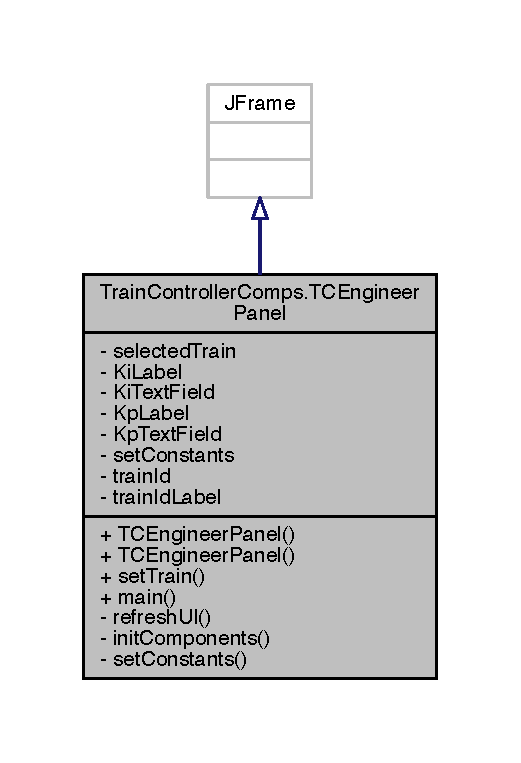
\includegraphics[width=250pt]{classTrainControllerComps_1_1TCEngineerPanel__inherit__graph}
\end{center}
\end{figure}


Collaboration diagram for Train\+Controller\+Comps.\+T\+C\+Engineer\+Panel\+:
\nopagebreak
\begin{figure}[H]
\begin{center}
\leavevmode
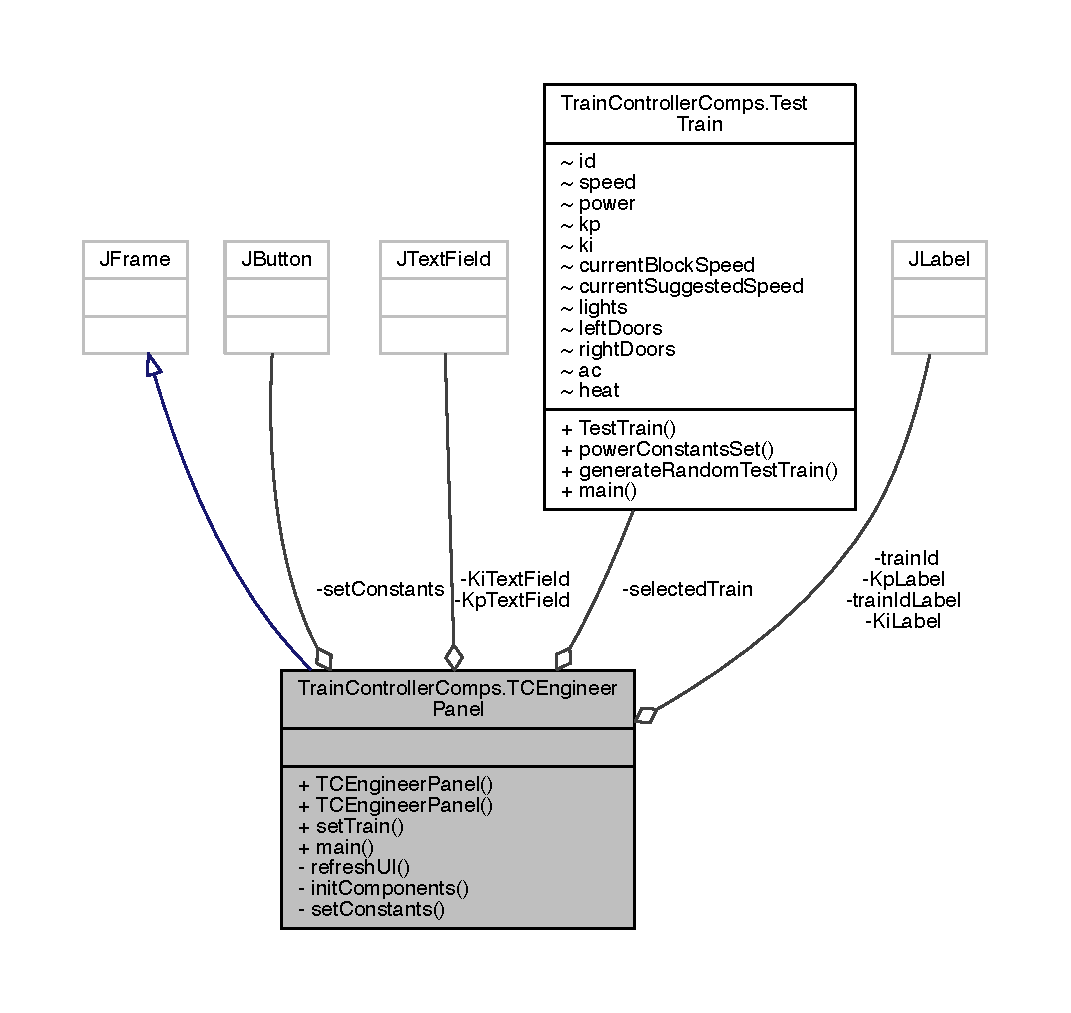
\includegraphics[width=350pt]{classTrainControllerComps_1_1TCEngineerPanel__coll__graph}
\end{center}
\end{figure}
\subsection*{Public Member Functions}
\begin{DoxyCompactItemize}
\item 
\hyperlink{classTrainControllerComps_1_1TCEngineerPanel_a5d8fd85270c170367dee1716ef758b21}{T\+C\+Engineer\+Panel} ()
\begin{DoxyCompactList}\small\item\em Constructor for creating a \hyperlink{classTrainControllerComps_1_1TCEngineerPanel}{T\+C\+Engineer\+Panel} object without any selected train. \end{DoxyCompactList}\item 
\hyperlink{classTrainControllerComps_1_1TCEngineerPanel_ad082ea6d180a9c420a1b474bc36d1127}{T\+C\+Engineer\+Panel} (\hyperlink{classTrainControllerComps_1_1TestTrain}{Test\+Train} \hyperlink{classtrain}{train})
\begin{DoxyCompactList}\small\item\em Constructor for creating a \hyperlink{classTrainControllerComps_1_1TCEngineerPanel}{T\+C\+Engineer\+Panel} object with a given train. \end{DoxyCompactList}\item 
void \hyperlink{classTrainControllerComps_1_1TCEngineerPanel_acf2325516cf881be1f635cc7bdbc4237}{set\+Train} (\hyperlink{classTrainControllerComps_1_1TestTrain}{Test\+Train} \hyperlink{classtrain}{train})
\begin{DoxyCompactList}\small\item\em Sets the train that the user wants to set the Kp and Ki for. \end{DoxyCompactList}\end{DoxyCompactItemize}
\subsection*{Static Public Member Functions}
\begin{DoxyCompactItemize}
\item 
static void \hyperlink{classTrainControllerComps_1_1TCEngineerPanel_a6803d6eb57e0d56c9d2fa5761d646b81}{main} (String args\mbox{[}$\,$\mbox{]})
\end{DoxyCompactItemize}
\subsection*{Private Member Functions}
\begin{DoxyCompactItemize}
\item 
void \hyperlink{classTrainControllerComps_1_1TCEngineerPanel_a9a2caf8e82d4e5107a9d509e2f8e9bab}{refresh\+UI} ()
\begin{DoxyCompactList}\small\item\em Refreshes the UI for the panel when a train is selected. \end{DoxyCompactList}\item 
void \hyperlink{classTrainControllerComps_1_1TCEngineerPanel_ac63c0a96eec1b142f085a0dd1bb6fd08}{init\+Components} ()
\begin{DoxyCompactList}\small\item\em This method is called from within the constructor to initialize the form. \end{DoxyCompactList}\item 
void \hyperlink{classTrainControllerComps_1_1TCEngineerPanel_ade4281b9ba79bf673f52bf43e6a1591b}{set\+Constants} (java.\+awt.\+event.\+Action\+Event evt)
\begin{DoxyCompactList}\small\item\em Gives the train the specified Kp and Ki that are in the text field. \end{DoxyCompactList}\end{DoxyCompactItemize}
\subsection*{Private Attributes}
\begin{DoxyCompactItemize}
\item 
\hyperlink{classTrainControllerComps_1_1TestTrain}{Test\+Train} \hyperlink{classTrainControllerComps_1_1TCEngineerPanel_a9950230a52e84c8ae3a3ebc577cfd016}{selected\+Train}
\begin{DoxyCompactList}\small\item\em The selected train whose power constants are being set. \end{DoxyCompactList}\item 
javax.\+swing.\+J\+Label \hyperlink{classTrainControllerComps_1_1TCEngineerPanel_ae0b00ead9378147b868dd7dd31fc0ec9}{Ki\+Label}
\item 
javax.\+swing.\+J\+Text\+Field \hyperlink{classTrainControllerComps_1_1TCEngineerPanel_a596fb9ed9f25ae8df3258652599bc3ca}{Ki\+Text\+Field}
\item 
javax.\+swing.\+J\+Label \hyperlink{classTrainControllerComps_1_1TCEngineerPanel_ab5cf30e22a542ee80bb725bdfca12df5}{Kp\+Label}
\item 
javax.\+swing.\+J\+Text\+Field \hyperlink{classTrainControllerComps_1_1TCEngineerPanel_a148b0b39f6a7c2aa6900223f2e586401}{Kp\+Text\+Field}
\item 
javax.\+swing.\+J\+Button \hyperlink{classTrainControllerComps_1_1TCEngineerPanel_a582de20717b9c5095c70421027e0b25b}{set\+Constants}
\item 
javax.\+swing.\+J\+Label \hyperlink{classTrainControllerComps_1_1TCEngineerPanel_a62a6ac9c5ed190fc132747fe8a3d9500}{train\+Id}
\item 
javax.\+swing.\+J\+Label \hyperlink{classTrainControllerComps_1_1TCEngineerPanel_a674c21e174fcd06d302dcc3ae23e1722}{train\+Id\+Label}
\end{DoxyCompactItemize}


\subsection{Detailed Description}
This class is responsible to set the Kp and Ki constants of a given train. 

This class collaborates with the Train Controller and the Train class.

\begin{DoxyAuthor}{Author}
Andrew Lendacky 
\end{DoxyAuthor}


\subsection{Constructor \& Destructor Documentation}
\mbox{\Hypertarget{classTrainControllerComps_1_1TCEngineerPanel_a5d8fd85270c170367dee1716ef758b21}\label{classTrainControllerComps_1_1TCEngineerPanel_a5d8fd85270c170367dee1716ef758b21}} 
\index{Train\+Controller\+Comps\+::\+T\+C\+Engineer\+Panel@{Train\+Controller\+Comps\+::\+T\+C\+Engineer\+Panel}!T\+C\+Engineer\+Panel@{T\+C\+Engineer\+Panel}}
\index{T\+C\+Engineer\+Panel@{T\+C\+Engineer\+Panel}!Train\+Controller\+Comps\+::\+T\+C\+Engineer\+Panel@{Train\+Controller\+Comps\+::\+T\+C\+Engineer\+Panel}}
\subsubsection{\texorpdfstring{T\+C\+Engineer\+Panel()}{TCEngineerPanel()}\hspace{0.1cm}{\footnotesize\ttfamily [1/2]}}
{\footnotesize\ttfamily Train\+Controller\+Comps.\+T\+C\+Engineer\+Panel.\+T\+C\+Engineer\+Panel (\begin{DoxyParamCaption}{ }\end{DoxyParamCaption})}



Constructor for creating a \hyperlink{classTrainControllerComps_1_1TCEngineerPanel}{T\+C\+Engineer\+Panel} object without any selected train. 

The selected train must be passed in by the Train Controller before being used. \mbox{\Hypertarget{classTrainControllerComps_1_1TCEngineerPanel_ad082ea6d180a9c420a1b474bc36d1127}\label{classTrainControllerComps_1_1TCEngineerPanel_ad082ea6d180a9c420a1b474bc36d1127}} 
\index{Train\+Controller\+Comps\+::\+T\+C\+Engineer\+Panel@{Train\+Controller\+Comps\+::\+T\+C\+Engineer\+Panel}!T\+C\+Engineer\+Panel@{T\+C\+Engineer\+Panel}}
\index{T\+C\+Engineer\+Panel@{T\+C\+Engineer\+Panel}!Train\+Controller\+Comps\+::\+T\+C\+Engineer\+Panel@{Train\+Controller\+Comps\+::\+T\+C\+Engineer\+Panel}}
\subsubsection{\texorpdfstring{T\+C\+Engineer\+Panel()}{TCEngineerPanel()}\hspace{0.1cm}{\footnotesize\ttfamily [2/2]}}
{\footnotesize\ttfamily Train\+Controller\+Comps.\+T\+C\+Engineer\+Panel.\+T\+C\+Engineer\+Panel (\begin{DoxyParamCaption}\item[{\hyperlink{classTrainControllerComps_1_1TestTrain}{Test\+Train}}]{train }\end{DoxyParamCaption})}



Constructor for creating a \hyperlink{classTrainControllerComps_1_1TCEngineerPanel}{T\+C\+Engineer\+Panel} object with a given train. 


\begin{DoxyParams}{Parameters}
{\em train} & the train controlled by the Train Controller. \\
\hline
\end{DoxyParams}


\subsection{Member Function Documentation}
\mbox{\Hypertarget{classTrainControllerComps_1_1TCEngineerPanel_ac63c0a96eec1b142f085a0dd1bb6fd08}\label{classTrainControllerComps_1_1TCEngineerPanel_ac63c0a96eec1b142f085a0dd1bb6fd08}} 
\index{Train\+Controller\+Comps\+::\+T\+C\+Engineer\+Panel@{Train\+Controller\+Comps\+::\+T\+C\+Engineer\+Panel}!init\+Components@{init\+Components}}
\index{init\+Components@{init\+Components}!Train\+Controller\+Comps\+::\+T\+C\+Engineer\+Panel@{Train\+Controller\+Comps\+::\+T\+C\+Engineer\+Panel}}
\subsubsection{\texorpdfstring{init\+Components()}{initComponents()}}
{\footnotesize\ttfamily void Train\+Controller\+Comps.\+T\+C\+Engineer\+Panel.\+init\+Components (\begin{DoxyParamCaption}{ }\end{DoxyParamCaption})\hspace{0.3cm}{\ttfamily [private]}}



This method is called from within the constructor to initialize the form. 

W\+A\+R\+N\+I\+NG\+: Do N\+OT modify this code. The content of this method is always regenerated by the Form Editor. \mbox{\Hypertarget{classTrainControllerComps_1_1TCEngineerPanel_a6803d6eb57e0d56c9d2fa5761d646b81}\label{classTrainControllerComps_1_1TCEngineerPanel_a6803d6eb57e0d56c9d2fa5761d646b81}} 
\index{Train\+Controller\+Comps\+::\+T\+C\+Engineer\+Panel@{Train\+Controller\+Comps\+::\+T\+C\+Engineer\+Panel}!main@{main}}
\index{main@{main}!Train\+Controller\+Comps\+::\+T\+C\+Engineer\+Panel@{Train\+Controller\+Comps\+::\+T\+C\+Engineer\+Panel}}
\subsubsection{\texorpdfstring{main()}{main()}}
{\footnotesize\ttfamily static void Train\+Controller\+Comps.\+T\+C\+Engineer\+Panel.\+main (\begin{DoxyParamCaption}\item[{String}]{args\mbox{[}$\,$\mbox{]} }\end{DoxyParamCaption})\hspace{0.3cm}{\ttfamily [static]}}


\begin{DoxyParams}{Parameters}
{\em args} & the command line arguments \\
\hline
\end{DoxyParams}
\mbox{\Hypertarget{classTrainControllerComps_1_1TCEngineerPanel_a9a2caf8e82d4e5107a9d509e2f8e9bab}\label{classTrainControllerComps_1_1TCEngineerPanel_a9a2caf8e82d4e5107a9d509e2f8e9bab}} 
\index{Train\+Controller\+Comps\+::\+T\+C\+Engineer\+Panel@{Train\+Controller\+Comps\+::\+T\+C\+Engineer\+Panel}!refresh\+UI@{refresh\+UI}}
\index{refresh\+UI@{refresh\+UI}!Train\+Controller\+Comps\+::\+T\+C\+Engineer\+Panel@{Train\+Controller\+Comps\+::\+T\+C\+Engineer\+Panel}}
\subsubsection{\texorpdfstring{refresh\+U\+I()}{refreshUI()}}
{\footnotesize\ttfamily void Train\+Controller\+Comps.\+T\+C\+Engineer\+Panel.\+refresh\+UI (\begin{DoxyParamCaption}{ }\end{DoxyParamCaption})\hspace{0.3cm}{\ttfamily [private]}}



Refreshes the UI for the panel when a train is selected. 

If a train already has a set Kp and Ki, it is displayed in the text fields If not the train has no set Kp and Ki, the text fields are set to 0.\+0. \mbox{\Hypertarget{classTrainControllerComps_1_1TCEngineerPanel_ade4281b9ba79bf673f52bf43e6a1591b}\label{classTrainControllerComps_1_1TCEngineerPanel_ade4281b9ba79bf673f52bf43e6a1591b}} 
\index{Train\+Controller\+Comps\+::\+T\+C\+Engineer\+Panel@{Train\+Controller\+Comps\+::\+T\+C\+Engineer\+Panel}!set\+Constants@{set\+Constants}}
\index{set\+Constants@{set\+Constants}!Train\+Controller\+Comps\+::\+T\+C\+Engineer\+Panel@{Train\+Controller\+Comps\+::\+T\+C\+Engineer\+Panel}}
\subsubsection{\texorpdfstring{set\+Constants()}{setConstants()}}
{\footnotesize\ttfamily void Train\+Controller\+Comps.\+T\+C\+Engineer\+Panel.\+set\+Constants (\begin{DoxyParamCaption}\item[{java.\+awt.\+event.\+Action\+Event}]{evt }\end{DoxyParamCaption})\hspace{0.3cm}{\ttfamily [private]}}



Gives the train the specified Kp and Ki that are in the text field. 

If the entries in the text field are not doubles, then an exception will be thrown, and the Kp and Ki will not be set.


\begin{DoxyParams}{Parameters}
{\em evt} & the sender of the event, i.\+e., the \char`\"{}\+Set\char`\"{} button. \\
\hline
\end{DoxyParams}
\mbox{\Hypertarget{classTrainControllerComps_1_1TCEngineerPanel_acf2325516cf881be1f635cc7bdbc4237}\label{classTrainControllerComps_1_1TCEngineerPanel_acf2325516cf881be1f635cc7bdbc4237}} 
\index{Train\+Controller\+Comps\+::\+T\+C\+Engineer\+Panel@{Train\+Controller\+Comps\+::\+T\+C\+Engineer\+Panel}!set\+Train@{set\+Train}}
\index{set\+Train@{set\+Train}!Train\+Controller\+Comps\+::\+T\+C\+Engineer\+Panel@{Train\+Controller\+Comps\+::\+T\+C\+Engineer\+Panel}}
\subsubsection{\texorpdfstring{set\+Train()}{setTrain()}}
{\footnotesize\ttfamily void Train\+Controller\+Comps.\+T\+C\+Engineer\+Panel.\+set\+Train (\begin{DoxyParamCaption}\item[{\hyperlink{classTrainControllerComps_1_1TestTrain}{Test\+Train}}]{train }\end{DoxyParamCaption})}



Sets the train that the user wants to set the Kp and Ki for. 


\begin{DoxyParams}{Parameters}
{\em train} & the train to control \\
\hline
\end{DoxyParams}


\subsection{Member Data Documentation}
\mbox{\Hypertarget{classTrainControllerComps_1_1TCEngineerPanel_ae0b00ead9378147b868dd7dd31fc0ec9}\label{classTrainControllerComps_1_1TCEngineerPanel_ae0b00ead9378147b868dd7dd31fc0ec9}} 
\index{Train\+Controller\+Comps\+::\+T\+C\+Engineer\+Panel@{Train\+Controller\+Comps\+::\+T\+C\+Engineer\+Panel}!Ki\+Label@{Ki\+Label}}
\index{Ki\+Label@{Ki\+Label}!Train\+Controller\+Comps\+::\+T\+C\+Engineer\+Panel@{Train\+Controller\+Comps\+::\+T\+C\+Engineer\+Panel}}
\subsubsection{\texorpdfstring{Ki\+Label}{KiLabel}}
{\footnotesize\ttfamily javax.\+swing.\+J\+Label Train\+Controller\+Comps.\+T\+C\+Engineer\+Panel.\+Ki\+Label\hspace{0.3cm}{\ttfamily [private]}}

\mbox{\Hypertarget{classTrainControllerComps_1_1TCEngineerPanel_a596fb9ed9f25ae8df3258652599bc3ca}\label{classTrainControllerComps_1_1TCEngineerPanel_a596fb9ed9f25ae8df3258652599bc3ca}} 
\index{Train\+Controller\+Comps\+::\+T\+C\+Engineer\+Panel@{Train\+Controller\+Comps\+::\+T\+C\+Engineer\+Panel}!Ki\+Text\+Field@{Ki\+Text\+Field}}
\index{Ki\+Text\+Field@{Ki\+Text\+Field}!Train\+Controller\+Comps\+::\+T\+C\+Engineer\+Panel@{Train\+Controller\+Comps\+::\+T\+C\+Engineer\+Panel}}
\subsubsection{\texorpdfstring{Ki\+Text\+Field}{KiTextField}}
{\footnotesize\ttfamily javax.\+swing.\+J\+Text\+Field Train\+Controller\+Comps.\+T\+C\+Engineer\+Panel.\+Ki\+Text\+Field\hspace{0.3cm}{\ttfamily [private]}}

\mbox{\Hypertarget{classTrainControllerComps_1_1TCEngineerPanel_ab5cf30e22a542ee80bb725bdfca12df5}\label{classTrainControllerComps_1_1TCEngineerPanel_ab5cf30e22a542ee80bb725bdfca12df5}} 
\index{Train\+Controller\+Comps\+::\+T\+C\+Engineer\+Panel@{Train\+Controller\+Comps\+::\+T\+C\+Engineer\+Panel}!Kp\+Label@{Kp\+Label}}
\index{Kp\+Label@{Kp\+Label}!Train\+Controller\+Comps\+::\+T\+C\+Engineer\+Panel@{Train\+Controller\+Comps\+::\+T\+C\+Engineer\+Panel}}
\subsubsection{\texorpdfstring{Kp\+Label}{KpLabel}}
{\footnotesize\ttfamily javax.\+swing.\+J\+Label Train\+Controller\+Comps.\+T\+C\+Engineer\+Panel.\+Kp\+Label\hspace{0.3cm}{\ttfamily [private]}}

\mbox{\Hypertarget{classTrainControllerComps_1_1TCEngineerPanel_a148b0b39f6a7c2aa6900223f2e586401}\label{classTrainControllerComps_1_1TCEngineerPanel_a148b0b39f6a7c2aa6900223f2e586401}} 
\index{Train\+Controller\+Comps\+::\+T\+C\+Engineer\+Panel@{Train\+Controller\+Comps\+::\+T\+C\+Engineer\+Panel}!Kp\+Text\+Field@{Kp\+Text\+Field}}
\index{Kp\+Text\+Field@{Kp\+Text\+Field}!Train\+Controller\+Comps\+::\+T\+C\+Engineer\+Panel@{Train\+Controller\+Comps\+::\+T\+C\+Engineer\+Panel}}
\subsubsection{\texorpdfstring{Kp\+Text\+Field}{KpTextField}}
{\footnotesize\ttfamily javax.\+swing.\+J\+Text\+Field Train\+Controller\+Comps.\+T\+C\+Engineer\+Panel.\+Kp\+Text\+Field\hspace{0.3cm}{\ttfamily [private]}}

\mbox{\Hypertarget{classTrainControllerComps_1_1TCEngineerPanel_a9950230a52e84c8ae3a3ebc577cfd016}\label{classTrainControllerComps_1_1TCEngineerPanel_a9950230a52e84c8ae3a3ebc577cfd016}} 
\index{Train\+Controller\+Comps\+::\+T\+C\+Engineer\+Panel@{Train\+Controller\+Comps\+::\+T\+C\+Engineer\+Panel}!selected\+Train@{selected\+Train}}
\index{selected\+Train@{selected\+Train}!Train\+Controller\+Comps\+::\+T\+C\+Engineer\+Panel@{Train\+Controller\+Comps\+::\+T\+C\+Engineer\+Panel}}
\subsubsection{\texorpdfstring{selected\+Train}{selectedTrain}}
{\footnotesize\ttfamily \hyperlink{classTrainControllerComps_1_1TestTrain}{Test\+Train} Train\+Controller\+Comps.\+T\+C\+Engineer\+Panel.\+selected\+Train\hspace{0.3cm}{\ttfamily [private]}}



The selected train whose power constants are being set. 

This train corresponds to the train that is being controlled by the Train Controller. \mbox{\Hypertarget{classTrainControllerComps_1_1TCEngineerPanel_a582de20717b9c5095c70421027e0b25b}\label{classTrainControllerComps_1_1TCEngineerPanel_a582de20717b9c5095c70421027e0b25b}} 
\index{Train\+Controller\+Comps\+::\+T\+C\+Engineer\+Panel@{Train\+Controller\+Comps\+::\+T\+C\+Engineer\+Panel}!set\+Constants@{set\+Constants}}
\index{set\+Constants@{set\+Constants}!Train\+Controller\+Comps\+::\+T\+C\+Engineer\+Panel@{Train\+Controller\+Comps\+::\+T\+C\+Engineer\+Panel}}
\subsubsection{\texorpdfstring{set\+Constants}{setConstants}}
{\footnotesize\ttfamily javax.\+swing.\+J\+Button Train\+Controller\+Comps.\+T\+C\+Engineer\+Panel.\+set\+Constants\hspace{0.3cm}{\ttfamily [private]}}

\mbox{\Hypertarget{classTrainControllerComps_1_1TCEngineerPanel_a62a6ac9c5ed190fc132747fe8a3d9500}\label{classTrainControllerComps_1_1TCEngineerPanel_a62a6ac9c5ed190fc132747fe8a3d9500}} 
\index{Train\+Controller\+Comps\+::\+T\+C\+Engineer\+Panel@{Train\+Controller\+Comps\+::\+T\+C\+Engineer\+Panel}!train\+Id@{train\+Id}}
\index{train\+Id@{train\+Id}!Train\+Controller\+Comps\+::\+T\+C\+Engineer\+Panel@{Train\+Controller\+Comps\+::\+T\+C\+Engineer\+Panel}}
\subsubsection{\texorpdfstring{train\+Id}{trainId}}
{\footnotesize\ttfamily javax.\+swing.\+J\+Label Train\+Controller\+Comps.\+T\+C\+Engineer\+Panel.\+train\+Id\hspace{0.3cm}{\ttfamily [private]}}

\mbox{\Hypertarget{classTrainControllerComps_1_1TCEngineerPanel_a674c21e174fcd06d302dcc3ae23e1722}\label{classTrainControllerComps_1_1TCEngineerPanel_a674c21e174fcd06d302dcc3ae23e1722}} 
\index{Train\+Controller\+Comps\+::\+T\+C\+Engineer\+Panel@{Train\+Controller\+Comps\+::\+T\+C\+Engineer\+Panel}!train\+Id\+Label@{train\+Id\+Label}}
\index{train\+Id\+Label@{train\+Id\+Label}!Train\+Controller\+Comps\+::\+T\+C\+Engineer\+Panel@{Train\+Controller\+Comps\+::\+T\+C\+Engineer\+Panel}}
\subsubsection{\texorpdfstring{train\+Id\+Label}{trainIdLabel}}
{\footnotesize\ttfamily javax.\+swing.\+J\+Label Train\+Controller\+Comps.\+T\+C\+Engineer\+Panel.\+train\+Id\+Label\hspace{0.3cm}{\ttfamily [private]}}



The documentation for this class was generated from the following file\+:\begin{DoxyCompactItemize}
\item 
src/main/java/\+Train\+Controller\+Comps/\hyperlink{TCEngineerPanel_8java}{T\+C\+Engineer\+Panel.\+java}\end{DoxyCompactItemize}

\hypertarget{classTrainControllerComps_1_1TCFailures}{}\section{Train\+Controller\+Comps.\+T\+C\+Failures Class Reference}
\label{classTrainControllerComps_1_1TCFailures}\index{Train\+Controller\+Comps.\+T\+C\+Failures@{Train\+Controller\+Comps.\+T\+C\+Failures}}


This class is responsible for display the states of the 3 failures that can occur on the train, as well as sending a signal to the C\+TC to repair the broken systems.  




Inheritance diagram for Train\+Controller\+Comps.\+T\+C\+Failures\+:
\nopagebreak
\begin{figure}[H]
\begin{center}
\leavevmode
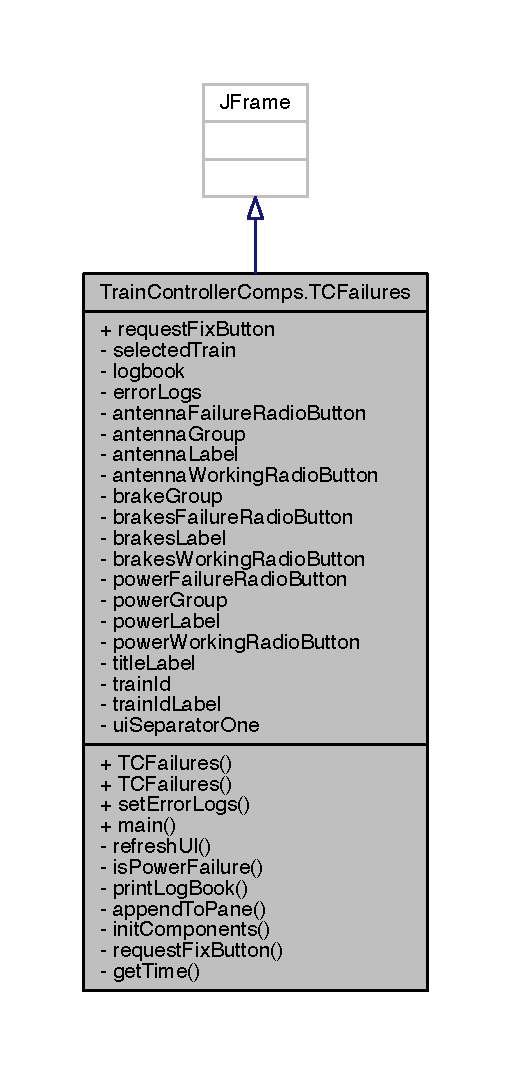
\includegraphics[width=245pt]{classTrainControllerComps_1_1TCFailures__inherit__graph}
\end{center}
\end{figure}


Collaboration diagram for Train\+Controller\+Comps.\+T\+C\+Failures\+:
\nopagebreak
\begin{figure}[H]
\begin{center}
\leavevmode
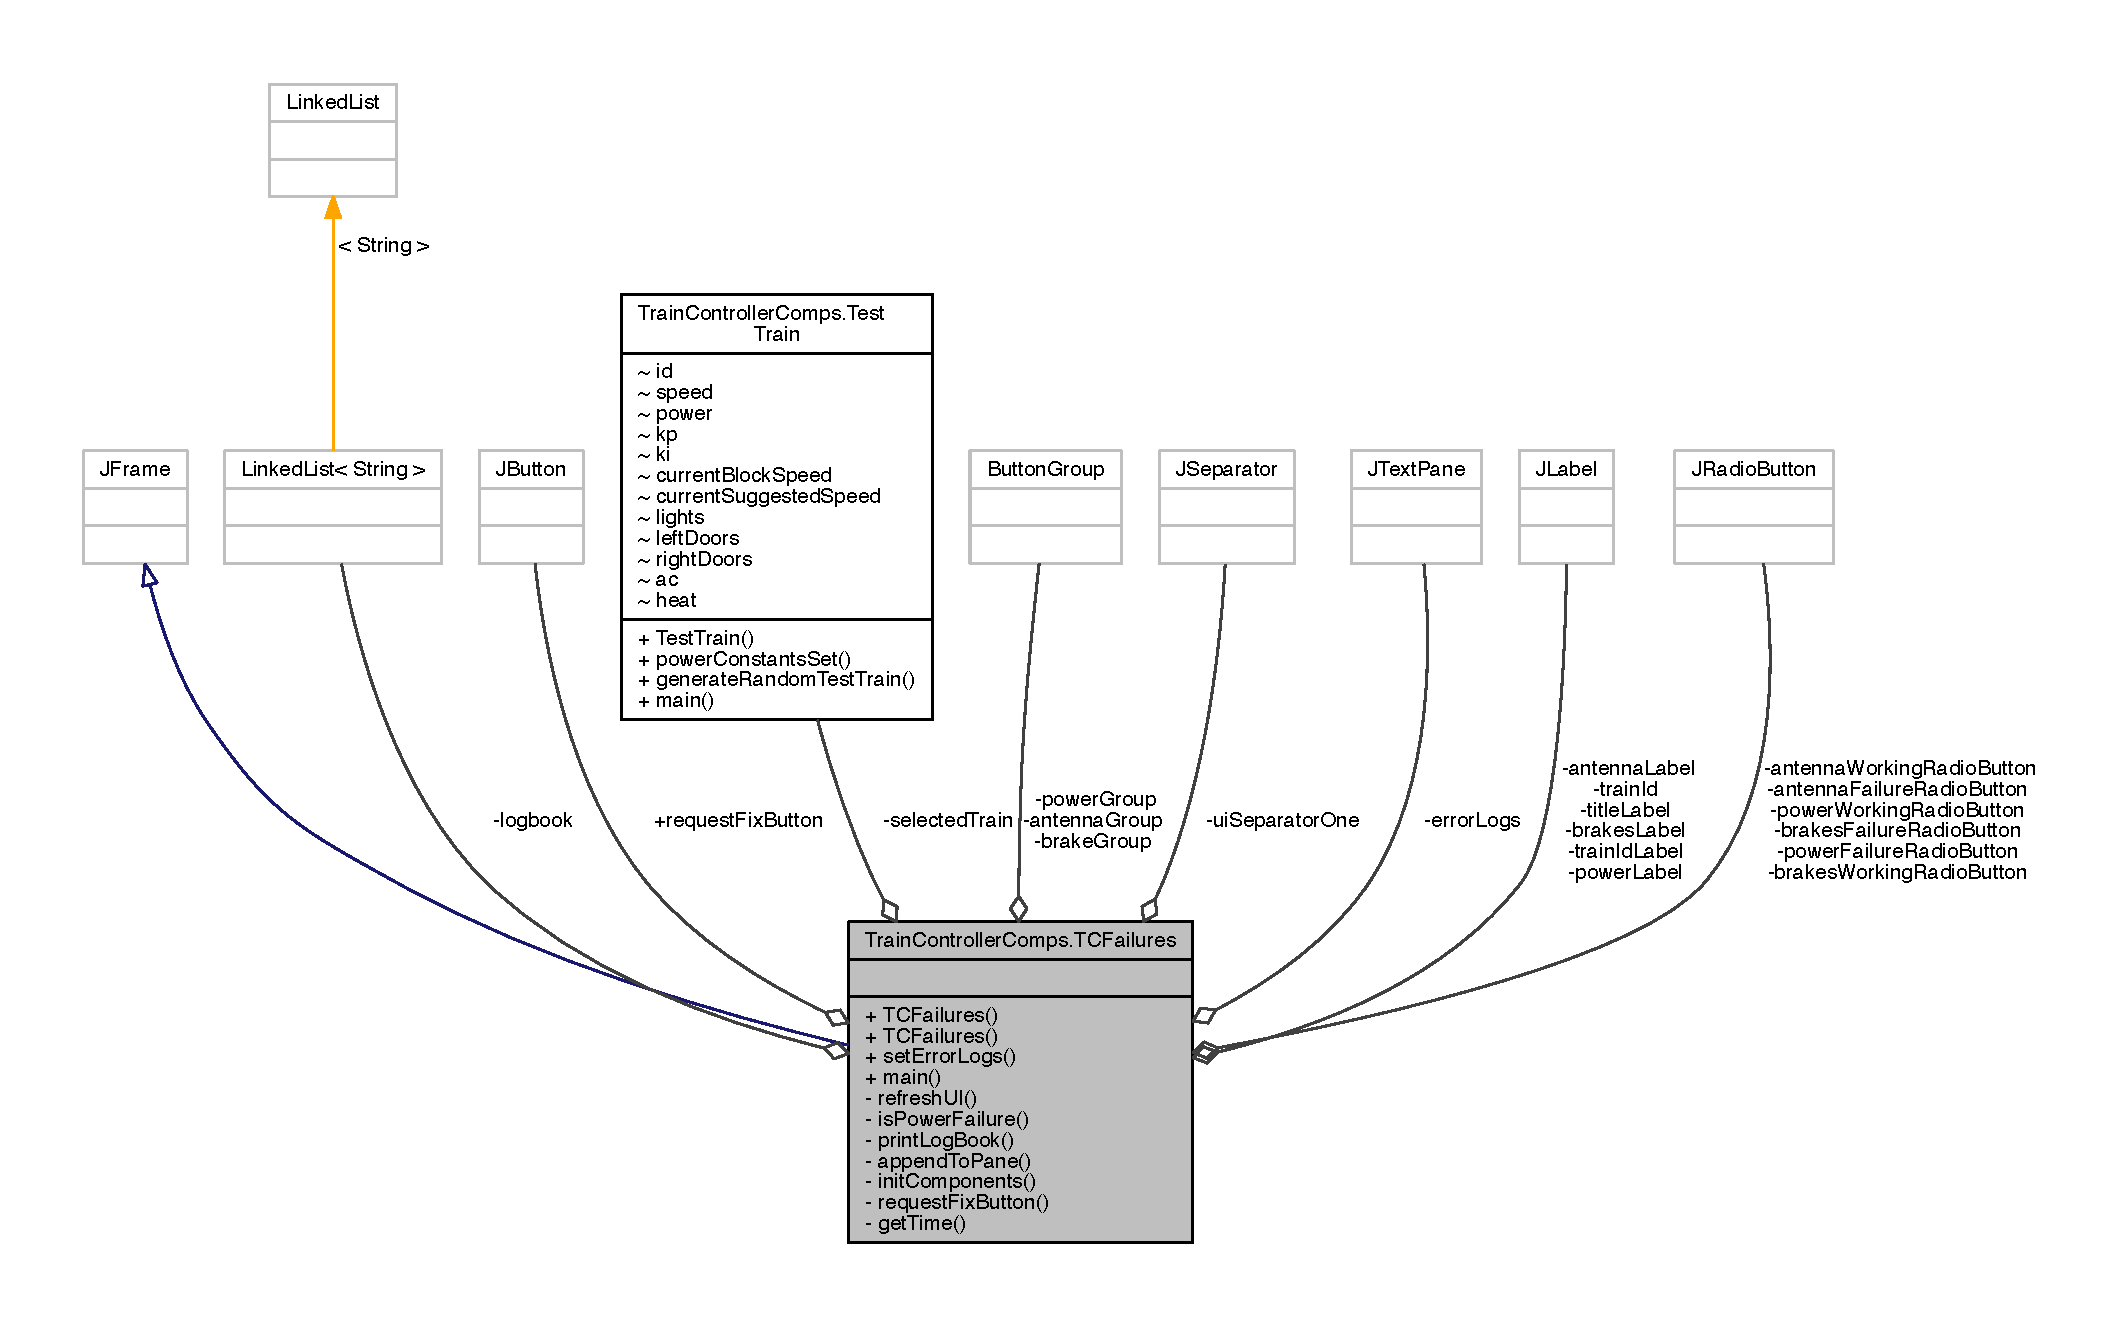
\includegraphics[width=350pt]{classTrainControllerComps_1_1TCFailures__coll__graph}
\end{center}
\end{figure}
\subsection*{Public Member Functions}
\begin{DoxyCompactItemize}
\item 
\hyperlink{classTrainControllerComps_1_1TCFailures_afbf09a8c516634c2376901ca04bebae9}{T\+C\+Failures} ()
\begin{DoxyCompactList}\small\item\em Constructor for creating a T\+C\+Failure object with no selected train, logbook, or error log. \end{DoxyCompactList}\item 
\hyperlink{classTrainControllerComps_1_1TCFailures_a021613d630232111e9a30398d15dcd51}{T\+C\+Failures} (\hyperlink{classTrainControllerComps_1_1TestTrain}{Test\+Train} \hyperlink{classtrain}{train})
\begin{DoxyCompactList}\small\item\em Constructor for creating a \hyperlink{classTrainControllerComps_1_1TCFailures}{T\+C\+Failures} object with a given train. \end{DoxyCompactList}\item 
void \hyperlink{classTrainControllerComps_1_1TCFailures_a9ce6a8fde30a39507e3ee5dfb1a02ba3}{set\+Error\+Logs} (J\+Text\+Pane err\+Log)
\begin{DoxyCompactList}\small\item\em Sets the error log that is to be printed to. \end{DoxyCompactList}\end{DoxyCompactItemize}
\subsection*{Static Public Member Functions}
\begin{DoxyCompactItemize}
\item 
static void \hyperlink{classTrainControllerComps_1_1TCFailures_a6c248a0171ceab80ac94ea966e97d5ba}{main} (String args\mbox{[}$\,$\mbox{]})
\end{DoxyCompactItemize}
\subsection*{Public Attributes}
\begin{DoxyCompactItemize}
\item 
javax.\+swing.\+J\+Button \hyperlink{classTrainControllerComps_1_1TCFailures_a0759ba38c88b24a362214722ef0dbfa7}{request\+Fix\+Button}
\end{DoxyCompactItemize}
\subsection*{Private Member Functions}
\begin{DoxyCompactItemize}
\item 
void \hyperlink{classTrainControllerComps_1_1TCFailures_ac2b39b97af1de62e3c73a74d2b7a20e1}{refresh\+UI} ()
\begin{DoxyCompactList}\small\item\em This method is not called from anywhere else, so the window does not refresh itself when a train has been fixed. \end{DoxyCompactList}\item 
boolean \hyperlink{classTrainControllerComps_1_1TCFailures_ab4d70425a3e693a1e21462deb74c8d6b}{is\+Power\+Failure} ()
\begin{DoxyCompactList}\small\item\em Checks if at least one of the utilities on the train is in a failure state, i.\+e., a power failure. \end{DoxyCompactList}\item 
void \hyperlink{classTrainControllerComps_1_1TCFailures_a0e826ca632b3289ad5b68ca93bb2fd11}{print\+Log\+Book} ()
\begin{DoxyCompactList}\small\item\em Prints the stored up logs from the logbook to the error log, and then clears the logbook. \end{DoxyCompactList}\item 
void \hyperlink{classTrainControllerComps_1_1TCFailures_a258e2032358c8398ea01b0feab32bcd6}{append\+To\+Pane} (J\+Text\+Pane tp, String msg, Color c)
\begin{DoxyCompactList}\small\item\em Add to a given log a given message in a given color. \end{DoxyCompactList}\item 
void \hyperlink{classTrainControllerComps_1_1TCFailures_abb8526b0ea750ed8d0570ae2e42713f8}{init\+Components} ()
\begin{DoxyCompactList}\small\item\em This method is called from within the constructor to initialize the form. \end{DoxyCompactList}\item 
void \hyperlink{classTrainControllerComps_1_1TCFailures_a16da0e026327d523cdcb1f4b9286e30a}{request\+Fix\+Button} (java.\+awt.\+event.\+Action\+Event evt)
\begin{DoxyCompactList}\small\item\em Requests a fix to the C\+TC if there is an Antenna, Power, or Brake Failure, and records it to the error log. \end{DoxyCompactList}\item 
String \hyperlink{classTrainControllerComps_1_1TCFailures_aeed3df89a5204c89c00e75174f8722aa}{get\+Time} ()
\begin{DoxyCompactList}\small\item\em Gets the time from the Operating System as a String. \end{DoxyCompactList}\end{DoxyCompactItemize}
\subsection*{Private Attributes}
\begin{DoxyCompactItemize}
\item 
\hyperlink{classTrainControllerComps_1_1TestTrain}{Test\+Train} \hyperlink{classTrainControllerComps_1_1TCFailures_a65fcb53be7a441d6ceec8872955ad8d7}{selected\+Train}
\begin{DoxyCompactList}\small\item\em The train in which to display the failures from. \end{DoxyCompactList}\item 
Linked\+List$<$ String $>$ \hyperlink{classTrainControllerComps_1_1TCFailures_a0c73c29afaca67760bd6b130ccbf2d4c}{logbook}
\begin{DoxyCompactList}\small\item\em A list to store up messages to print to the error log. \end{DoxyCompactList}\item 
J\+Text\+Pane \hyperlink{classTrainControllerComps_1_1TCFailures_a07b6a5403f60a1e2e6510836de30d906}{error\+Logs}
\begin{DoxyCompactList}\small\item\em Area to print the error logs to. \end{DoxyCompactList}\item 
javax.\+swing.\+J\+Radio\+Button \hyperlink{classTrainControllerComps_1_1TCFailures_ac74d2657306216535068bd17548b9661}{antenna\+Failure\+Radio\+Button}
\item 
javax.\+swing.\+Button\+Group \hyperlink{classTrainControllerComps_1_1TCFailures_a8c7e61b0b03ba87a123c5d9277b13af3}{antenna\+Group}
\item 
javax.\+swing.\+J\+Label \hyperlink{classTrainControllerComps_1_1TCFailures_a93e714edc703ad8ddb8ea9e869443ad7}{antenna\+Label}
\item 
javax.\+swing.\+J\+Radio\+Button \hyperlink{classTrainControllerComps_1_1TCFailures_a42b774e2408469ae3ba0d62839f88a42}{antenna\+Working\+Radio\+Button}
\item 
javax.\+swing.\+Button\+Group \hyperlink{classTrainControllerComps_1_1TCFailures_a6c7510f746275475950bf30eba68cae8}{brake\+Group}
\item 
javax.\+swing.\+J\+Radio\+Button \hyperlink{classTrainControllerComps_1_1TCFailures_af6a949a714e480c7895ea3bfc888a098}{brakes\+Failure\+Radio\+Button}
\item 
javax.\+swing.\+J\+Label \hyperlink{classTrainControllerComps_1_1TCFailures_ab57a4712aba9bf053d7cbedfaca730e5}{brakes\+Label}
\item 
javax.\+swing.\+J\+Radio\+Button \hyperlink{classTrainControllerComps_1_1TCFailures_a248c5a31df39bfb278e59da0b4641b40}{brakes\+Working\+Radio\+Button}
\item 
javax.\+swing.\+J\+Radio\+Button \hyperlink{classTrainControllerComps_1_1TCFailures_a66d3a69d8c53976528fa025cb0acef2c}{power\+Failure\+Radio\+Button}
\item 
javax.\+swing.\+Button\+Group \hyperlink{classTrainControllerComps_1_1TCFailures_a28320b6b09f3dfb2f7906d24cdc2cb92}{power\+Group}
\item 
javax.\+swing.\+J\+Label \hyperlink{classTrainControllerComps_1_1TCFailures_a567ab26c57cbd96117393bd3ce4958f1}{power\+Label}
\item 
javax.\+swing.\+J\+Radio\+Button \hyperlink{classTrainControllerComps_1_1TCFailures_a1801a3cc7ab2a87605497f7d5fb96acd}{power\+Working\+Radio\+Button}
\item 
javax.\+swing.\+J\+Label \hyperlink{classTrainControllerComps_1_1TCFailures_a58b8932f973472f4199f77e5d2eaaf14}{title\+Label}
\item 
javax.\+swing.\+J\+Label \hyperlink{classTrainControllerComps_1_1TCFailures_ada89c81b5d3fb48652c5f542431dc3da}{train\+Id}
\item 
javax.\+swing.\+J\+Label \hyperlink{classTrainControllerComps_1_1TCFailures_aeee00ebb3eb979b4916d3cf8294c1e59}{train\+Id\+Label}
\item 
javax.\+swing.\+J\+Separator \hyperlink{classTrainControllerComps_1_1TCFailures_addc1377b0e7ab921bba464c9892593e6}{ui\+Separator\+One}
\end{DoxyCompactItemize}


\subsection{Detailed Description}
This class is responsible for display the states of the 3 failures that can occur on the train, as well as sending a signal to the C\+TC to repair the broken systems. 

The three failures are\+: antenna, power, and brake.

This class collaborates with the Train Controller and Train class.

\begin{DoxyAuthor}{Author}
Andrew Lendacky 
\end{DoxyAuthor}


\subsection{Constructor \& Destructor Documentation}
\mbox{\Hypertarget{classTrainControllerComps_1_1TCFailures_afbf09a8c516634c2376901ca04bebae9}\label{classTrainControllerComps_1_1TCFailures_afbf09a8c516634c2376901ca04bebae9}} 
\index{Train\+Controller\+Comps\+::\+T\+C\+Failures@{Train\+Controller\+Comps\+::\+T\+C\+Failures}!T\+C\+Failures@{T\+C\+Failures}}
\index{T\+C\+Failures@{T\+C\+Failures}!Train\+Controller\+Comps\+::\+T\+C\+Failures@{Train\+Controller\+Comps\+::\+T\+C\+Failures}}
\subsubsection{\texorpdfstring{T\+C\+Failures()}{TCFailures()}\hspace{0.1cm}{\footnotesize\ttfamily [1/2]}}
{\footnotesize\ttfamily Train\+Controller\+Comps.\+T\+C\+Failures.\+T\+C\+Failures (\begin{DoxyParamCaption}{ }\end{DoxyParamCaption})}



Constructor for creating a T\+C\+Failure object with no selected train, logbook, or error log. 

These must be passed in from the Train Controller before being used. \mbox{\Hypertarget{classTrainControllerComps_1_1TCFailures_a021613d630232111e9a30398d15dcd51}\label{classTrainControllerComps_1_1TCFailures_a021613d630232111e9a30398d15dcd51}} 
\index{Train\+Controller\+Comps\+::\+T\+C\+Failures@{Train\+Controller\+Comps\+::\+T\+C\+Failures}!T\+C\+Failures@{T\+C\+Failures}}
\index{T\+C\+Failures@{T\+C\+Failures}!Train\+Controller\+Comps\+::\+T\+C\+Failures@{Train\+Controller\+Comps\+::\+T\+C\+Failures}}
\subsubsection{\texorpdfstring{T\+C\+Failures()}{TCFailures()}\hspace{0.1cm}{\footnotesize\ttfamily [2/2]}}
{\footnotesize\ttfamily Train\+Controller\+Comps.\+T\+C\+Failures.\+T\+C\+Failures (\begin{DoxyParamCaption}\item[{\hyperlink{classTrainControllerComps_1_1TestTrain}{Test\+Train}}]{train }\end{DoxyParamCaption})}



Constructor for creating a \hyperlink{classTrainControllerComps_1_1TCFailures}{T\+C\+Failures} object with a given train. 


\begin{DoxyParams}{Parameters}
{\em train} & the selected train from the Train Controller \\
\hline
\end{DoxyParams}


\subsection{Member Function Documentation}
\mbox{\Hypertarget{classTrainControllerComps_1_1TCFailures_a258e2032358c8398ea01b0feab32bcd6}\label{classTrainControllerComps_1_1TCFailures_a258e2032358c8398ea01b0feab32bcd6}} 
\index{Train\+Controller\+Comps\+::\+T\+C\+Failures@{Train\+Controller\+Comps\+::\+T\+C\+Failures}!append\+To\+Pane@{append\+To\+Pane}}
\index{append\+To\+Pane@{append\+To\+Pane}!Train\+Controller\+Comps\+::\+T\+C\+Failures@{Train\+Controller\+Comps\+::\+T\+C\+Failures}}
\subsubsection{\texorpdfstring{append\+To\+Pane()}{appendToPane()}}
{\footnotesize\ttfamily void Train\+Controller\+Comps.\+T\+C\+Failures.\+append\+To\+Pane (\begin{DoxyParamCaption}\item[{J\+Text\+Pane}]{tp,  }\item[{String}]{msg,  }\item[{Color}]{c }\end{DoxyParamCaption})\hspace{0.3cm}{\ttfamily [private]}}



Add to a given log a given message in a given color. 


\begin{DoxyParams}{Parameters}
{\em tp} & the text pane to display the message in. \\
\hline
{\em msg} & the message to display. \\
\hline
{\em c} & the color to display the message in. \\
\hline
\end{DoxyParams}
\mbox{\Hypertarget{classTrainControllerComps_1_1TCFailures_aeed3df89a5204c89c00e75174f8722aa}\label{classTrainControllerComps_1_1TCFailures_aeed3df89a5204c89c00e75174f8722aa}} 
\index{Train\+Controller\+Comps\+::\+T\+C\+Failures@{Train\+Controller\+Comps\+::\+T\+C\+Failures}!get\+Time@{get\+Time}}
\index{get\+Time@{get\+Time}!Train\+Controller\+Comps\+::\+T\+C\+Failures@{Train\+Controller\+Comps\+::\+T\+C\+Failures}}
\subsubsection{\texorpdfstring{get\+Time()}{getTime()}}
{\footnotesize\ttfamily String Train\+Controller\+Comps.\+T\+C\+Failures.\+get\+Time (\begin{DoxyParamCaption}{ }\end{DoxyParamCaption})\hspace{0.3cm}{\ttfamily [private]}}



Gets the time from the Operating System as a String. 

\begin{DoxyReturn}{Returns}
returns the time of the system. 
\end{DoxyReturn}
\mbox{\Hypertarget{classTrainControllerComps_1_1TCFailures_abb8526b0ea750ed8d0570ae2e42713f8}\label{classTrainControllerComps_1_1TCFailures_abb8526b0ea750ed8d0570ae2e42713f8}} 
\index{Train\+Controller\+Comps\+::\+T\+C\+Failures@{Train\+Controller\+Comps\+::\+T\+C\+Failures}!init\+Components@{init\+Components}}
\index{init\+Components@{init\+Components}!Train\+Controller\+Comps\+::\+T\+C\+Failures@{Train\+Controller\+Comps\+::\+T\+C\+Failures}}
\subsubsection{\texorpdfstring{init\+Components()}{initComponents()}}
{\footnotesize\ttfamily void Train\+Controller\+Comps.\+T\+C\+Failures.\+init\+Components (\begin{DoxyParamCaption}{ }\end{DoxyParamCaption})\hspace{0.3cm}{\ttfamily [private]}}



This method is called from within the constructor to initialize the form. 

W\+A\+R\+N\+I\+NG\+: Do N\+OT modify this code. The content of this method is always regenerated by the Form Editor. \mbox{\Hypertarget{classTrainControllerComps_1_1TCFailures_ab4d70425a3e693a1e21462deb74c8d6b}\label{classTrainControllerComps_1_1TCFailures_ab4d70425a3e693a1e21462deb74c8d6b}} 
\index{Train\+Controller\+Comps\+::\+T\+C\+Failures@{Train\+Controller\+Comps\+::\+T\+C\+Failures}!is\+Power\+Failure@{is\+Power\+Failure}}
\index{is\+Power\+Failure@{is\+Power\+Failure}!Train\+Controller\+Comps\+::\+T\+C\+Failures@{Train\+Controller\+Comps\+::\+T\+C\+Failures}}
\subsubsection{\texorpdfstring{is\+Power\+Failure()}{isPowerFailure()}}
{\footnotesize\ttfamily boolean Train\+Controller\+Comps.\+T\+C\+Failures.\+is\+Power\+Failure (\begin{DoxyParamCaption}{ }\end{DoxyParamCaption})\hspace{0.3cm}{\ttfamily [private]}}



Checks if at least one of the utilities on the train is in a failure state, i.\+e., a power failure. 

\begin{DoxyReturn}{Returns}
returns true if there is at least one utility broken, false if all the utilities are working. 
\end{DoxyReturn}
\mbox{\Hypertarget{classTrainControllerComps_1_1TCFailures_a6c248a0171ceab80ac94ea966e97d5ba}\label{classTrainControllerComps_1_1TCFailures_a6c248a0171ceab80ac94ea966e97d5ba}} 
\index{Train\+Controller\+Comps\+::\+T\+C\+Failures@{Train\+Controller\+Comps\+::\+T\+C\+Failures}!main@{main}}
\index{main@{main}!Train\+Controller\+Comps\+::\+T\+C\+Failures@{Train\+Controller\+Comps\+::\+T\+C\+Failures}}
\subsubsection{\texorpdfstring{main()}{main()}}
{\footnotesize\ttfamily static void Train\+Controller\+Comps.\+T\+C\+Failures.\+main (\begin{DoxyParamCaption}\item[{String}]{args\mbox{[}$\,$\mbox{]} }\end{DoxyParamCaption})\hspace{0.3cm}{\ttfamily [static]}}


\begin{DoxyParams}{Parameters}
{\em args} & the command line arguments \\
\hline
\end{DoxyParams}
\mbox{\Hypertarget{classTrainControllerComps_1_1TCFailures_a0e826ca632b3289ad5b68ca93bb2fd11}\label{classTrainControllerComps_1_1TCFailures_a0e826ca632b3289ad5b68ca93bb2fd11}} 
\index{Train\+Controller\+Comps\+::\+T\+C\+Failures@{Train\+Controller\+Comps\+::\+T\+C\+Failures}!print\+Log\+Book@{print\+Log\+Book}}
\index{print\+Log\+Book@{print\+Log\+Book}!Train\+Controller\+Comps\+::\+T\+C\+Failures@{Train\+Controller\+Comps\+::\+T\+C\+Failures}}
\subsubsection{\texorpdfstring{print\+Log\+Book()}{printLogBook()}}
{\footnotesize\ttfamily void Train\+Controller\+Comps.\+T\+C\+Failures.\+print\+Log\+Book (\begin{DoxyParamCaption}{ }\end{DoxyParamCaption})\hspace{0.3cm}{\ttfamily [private]}}



Prints the stored up logs from the logbook to the error log, and then clears the logbook. 

\mbox{\Hypertarget{classTrainControllerComps_1_1TCFailures_ac2b39b97af1de62e3c73a74d2b7a20e1}\label{classTrainControllerComps_1_1TCFailures_ac2b39b97af1de62e3c73a74d2b7a20e1}} 
\index{Train\+Controller\+Comps\+::\+T\+C\+Failures@{Train\+Controller\+Comps\+::\+T\+C\+Failures}!refresh\+UI@{refresh\+UI}}
\index{refresh\+UI@{refresh\+UI}!Train\+Controller\+Comps\+::\+T\+C\+Failures@{Train\+Controller\+Comps\+::\+T\+C\+Failures}}
\subsubsection{\texorpdfstring{refresh\+U\+I()}{refreshUI()}}
{\footnotesize\ttfamily void Train\+Controller\+Comps.\+T\+C\+Failures.\+refresh\+UI (\begin{DoxyParamCaption}{ }\end{DoxyParamCaption})\hspace{0.3cm}{\ttfamily [private]}}



This method is not called from anywhere else, so the window does not refresh itself when a train has been fixed. 

Therefore, it will continue to show the old states of the failures until the user closes the window and reopens it. Refreshes the UI to update the radio buttons based on the status of the train. \mbox{\Hypertarget{classTrainControllerComps_1_1TCFailures_a16da0e026327d523cdcb1f4b9286e30a}\label{classTrainControllerComps_1_1TCFailures_a16da0e026327d523cdcb1f4b9286e30a}} 
\index{Train\+Controller\+Comps\+::\+T\+C\+Failures@{Train\+Controller\+Comps\+::\+T\+C\+Failures}!request\+Fix\+Button@{request\+Fix\+Button}}
\index{request\+Fix\+Button@{request\+Fix\+Button}!Train\+Controller\+Comps\+::\+T\+C\+Failures@{Train\+Controller\+Comps\+::\+T\+C\+Failures}}
\subsubsection{\texorpdfstring{request\+Fix\+Button()}{requestFixButton()}}
{\footnotesize\ttfamily void Train\+Controller\+Comps.\+T\+C\+Failures.\+request\+Fix\+Button (\begin{DoxyParamCaption}\item[{java.\+awt.\+event.\+Action\+Event}]{evt }\end{DoxyParamCaption})\hspace{0.3cm}{\ttfamily [private]}}



Requests a fix to the C\+TC if there is an Antenna, Power, or Brake Failure, and records it to the error log. 


\begin{DoxyParams}{Parameters}
{\em evt} & the sender of the event, i.\+e., the \textquotesingle{}Request Fix\textquotesingle{} button. \\
\hline
\end{DoxyParams}
\mbox{\Hypertarget{classTrainControllerComps_1_1TCFailures_a9ce6a8fde30a39507e3ee5dfb1a02ba3}\label{classTrainControllerComps_1_1TCFailures_a9ce6a8fde30a39507e3ee5dfb1a02ba3}} 
\index{Train\+Controller\+Comps\+::\+T\+C\+Failures@{Train\+Controller\+Comps\+::\+T\+C\+Failures}!set\+Error\+Logs@{set\+Error\+Logs}}
\index{set\+Error\+Logs@{set\+Error\+Logs}!Train\+Controller\+Comps\+::\+T\+C\+Failures@{Train\+Controller\+Comps\+::\+T\+C\+Failures}}
\subsubsection{\texorpdfstring{set\+Error\+Logs()}{setErrorLogs()}}
{\footnotesize\ttfamily void Train\+Controller\+Comps.\+T\+C\+Failures.\+set\+Error\+Logs (\begin{DoxyParamCaption}\item[{J\+Text\+Pane}]{err\+Log }\end{DoxyParamCaption})}



Sets the error log that is to be printed to. 


\begin{DoxyParams}{Parameters}
{\em err\+Logs} & a textpane representing the error log \\
\hline
\end{DoxyParams}


\subsection{Member Data Documentation}
\mbox{\Hypertarget{classTrainControllerComps_1_1TCFailures_ac74d2657306216535068bd17548b9661}\label{classTrainControllerComps_1_1TCFailures_ac74d2657306216535068bd17548b9661}} 
\index{Train\+Controller\+Comps\+::\+T\+C\+Failures@{Train\+Controller\+Comps\+::\+T\+C\+Failures}!antenna\+Failure\+Radio\+Button@{antenna\+Failure\+Radio\+Button}}
\index{antenna\+Failure\+Radio\+Button@{antenna\+Failure\+Radio\+Button}!Train\+Controller\+Comps\+::\+T\+C\+Failures@{Train\+Controller\+Comps\+::\+T\+C\+Failures}}
\subsubsection{\texorpdfstring{antenna\+Failure\+Radio\+Button}{antennaFailureRadioButton}}
{\footnotesize\ttfamily javax.\+swing.\+J\+Radio\+Button Train\+Controller\+Comps.\+T\+C\+Failures.\+antenna\+Failure\+Radio\+Button\hspace{0.3cm}{\ttfamily [private]}}

\mbox{\Hypertarget{classTrainControllerComps_1_1TCFailures_a8c7e61b0b03ba87a123c5d9277b13af3}\label{classTrainControllerComps_1_1TCFailures_a8c7e61b0b03ba87a123c5d9277b13af3}} 
\index{Train\+Controller\+Comps\+::\+T\+C\+Failures@{Train\+Controller\+Comps\+::\+T\+C\+Failures}!antenna\+Group@{antenna\+Group}}
\index{antenna\+Group@{antenna\+Group}!Train\+Controller\+Comps\+::\+T\+C\+Failures@{Train\+Controller\+Comps\+::\+T\+C\+Failures}}
\subsubsection{\texorpdfstring{antenna\+Group}{antennaGroup}}
{\footnotesize\ttfamily javax.\+swing.\+Button\+Group Train\+Controller\+Comps.\+T\+C\+Failures.\+antenna\+Group\hspace{0.3cm}{\ttfamily [private]}}

\mbox{\Hypertarget{classTrainControllerComps_1_1TCFailures_a93e714edc703ad8ddb8ea9e869443ad7}\label{classTrainControllerComps_1_1TCFailures_a93e714edc703ad8ddb8ea9e869443ad7}} 
\index{Train\+Controller\+Comps\+::\+T\+C\+Failures@{Train\+Controller\+Comps\+::\+T\+C\+Failures}!antenna\+Label@{antenna\+Label}}
\index{antenna\+Label@{antenna\+Label}!Train\+Controller\+Comps\+::\+T\+C\+Failures@{Train\+Controller\+Comps\+::\+T\+C\+Failures}}
\subsubsection{\texorpdfstring{antenna\+Label}{antennaLabel}}
{\footnotesize\ttfamily javax.\+swing.\+J\+Label Train\+Controller\+Comps.\+T\+C\+Failures.\+antenna\+Label\hspace{0.3cm}{\ttfamily [private]}}

\mbox{\Hypertarget{classTrainControllerComps_1_1TCFailures_a42b774e2408469ae3ba0d62839f88a42}\label{classTrainControllerComps_1_1TCFailures_a42b774e2408469ae3ba0d62839f88a42}} 
\index{Train\+Controller\+Comps\+::\+T\+C\+Failures@{Train\+Controller\+Comps\+::\+T\+C\+Failures}!antenna\+Working\+Radio\+Button@{antenna\+Working\+Radio\+Button}}
\index{antenna\+Working\+Radio\+Button@{antenna\+Working\+Radio\+Button}!Train\+Controller\+Comps\+::\+T\+C\+Failures@{Train\+Controller\+Comps\+::\+T\+C\+Failures}}
\subsubsection{\texorpdfstring{antenna\+Working\+Radio\+Button}{antennaWorkingRadioButton}}
{\footnotesize\ttfamily javax.\+swing.\+J\+Radio\+Button Train\+Controller\+Comps.\+T\+C\+Failures.\+antenna\+Working\+Radio\+Button\hspace{0.3cm}{\ttfamily [private]}}

\mbox{\Hypertarget{classTrainControllerComps_1_1TCFailures_a6c7510f746275475950bf30eba68cae8}\label{classTrainControllerComps_1_1TCFailures_a6c7510f746275475950bf30eba68cae8}} 
\index{Train\+Controller\+Comps\+::\+T\+C\+Failures@{Train\+Controller\+Comps\+::\+T\+C\+Failures}!brake\+Group@{brake\+Group}}
\index{brake\+Group@{brake\+Group}!Train\+Controller\+Comps\+::\+T\+C\+Failures@{Train\+Controller\+Comps\+::\+T\+C\+Failures}}
\subsubsection{\texorpdfstring{brake\+Group}{brakeGroup}}
{\footnotesize\ttfamily javax.\+swing.\+Button\+Group Train\+Controller\+Comps.\+T\+C\+Failures.\+brake\+Group\hspace{0.3cm}{\ttfamily [private]}}

\mbox{\Hypertarget{classTrainControllerComps_1_1TCFailures_af6a949a714e480c7895ea3bfc888a098}\label{classTrainControllerComps_1_1TCFailures_af6a949a714e480c7895ea3bfc888a098}} 
\index{Train\+Controller\+Comps\+::\+T\+C\+Failures@{Train\+Controller\+Comps\+::\+T\+C\+Failures}!brakes\+Failure\+Radio\+Button@{brakes\+Failure\+Radio\+Button}}
\index{brakes\+Failure\+Radio\+Button@{brakes\+Failure\+Radio\+Button}!Train\+Controller\+Comps\+::\+T\+C\+Failures@{Train\+Controller\+Comps\+::\+T\+C\+Failures}}
\subsubsection{\texorpdfstring{brakes\+Failure\+Radio\+Button}{brakesFailureRadioButton}}
{\footnotesize\ttfamily javax.\+swing.\+J\+Radio\+Button Train\+Controller\+Comps.\+T\+C\+Failures.\+brakes\+Failure\+Radio\+Button\hspace{0.3cm}{\ttfamily [private]}}

\mbox{\Hypertarget{classTrainControllerComps_1_1TCFailures_ab57a4712aba9bf053d7cbedfaca730e5}\label{classTrainControllerComps_1_1TCFailures_ab57a4712aba9bf053d7cbedfaca730e5}} 
\index{Train\+Controller\+Comps\+::\+T\+C\+Failures@{Train\+Controller\+Comps\+::\+T\+C\+Failures}!brakes\+Label@{brakes\+Label}}
\index{brakes\+Label@{brakes\+Label}!Train\+Controller\+Comps\+::\+T\+C\+Failures@{Train\+Controller\+Comps\+::\+T\+C\+Failures}}
\subsubsection{\texorpdfstring{brakes\+Label}{brakesLabel}}
{\footnotesize\ttfamily javax.\+swing.\+J\+Label Train\+Controller\+Comps.\+T\+C\+Failures.\+brakes\+Label\hspace{0.3cm}{\ttfamily [private]}}

\mbox{\Hypertarget{classTrainControllerComps_1_1TCFailures_a248c5a31df39bfb278e59da0b4641b40}\label{classTrainControllerComps_1_1TCFailures_a248c5a31df39bfb278e59da0b4641b40}} 
\index{Train\+Controller\+Comps\+::\+T\+C\+Failures@{Train\+Controller\+Comps\+::\+T\+C\+Failures}!brakes\+Working\+Radio\+Button@{brakes\+Working\+Radio\+Button}}
\index{brakes\+Working\+Radio\+Button@{brakes\+Working\+Radio\+Button}!Train\+Controller\+Comps\+::\+T\+C\+Failures@{Train\+Controller\+Comps\+::\+T\+C\+Failures}}
\subsubsection{\texorpdfstring{brakes\+Working\+Radio\+Button}{brakesWorkingRadioButton}}
{\footnotesize\ttfamily javax.\+swing.\+J\+Radio\+Button Train\+Controller\+Comps.\+T\+C\+Failures.\+brakes\+Working\+Radio\+Button\hspace{0.3cm}{\ttfamily [private]}}

\mbox{\Hypertarget{classTrainControllerComps_1_1TCFailures_a07b6a5403f60a1e2e6510836de30d906}\label{classTrainControllerComps_1_1TCFailures_a07b6a5403f60a1e2e6510836de30d906}} 
\index{Train\+Controller\+Comps\+::\+T\+C\+Failures@{Train\+Controller\+Comps\+::\+T\+C\+Failures}!error\+Logs@{error\+Logs}}
\index{error\+Logs@{error\+Logs}!Train\+Controller\+Comps\+::\+T\+C\+Failures@{Train\+Controller\+Comps\+::\+T\+C\+Failures}}
\subsubsection{\texorpdfstring{error\+Logs}{errorLogs}}
{\footnotesize\ttfamily J\+Text\+Pane Train\+Controller\+Comps.\+T\+C\+Failures.\+error\+Logs\hspace{0.3cm}{\ttfamily [private]}}



Area to print the error logs to. 

This comes from the error\+Logs from the Train Controller class. \mbox{\Hypertarget{classTrainControllerComps_1_1TCFailures_a0c73c29afaca67760bd6b130ccbf2d4c}\label{classTrainControllerComps_1_1TCFailures_a0c73c29afaca67760bd6b130ccbf2d4c}} 
\index{Train\+Controller\+Comps\+::\+T\+C\+Failures@{Train\+Controller\+Comps\+::\+T\+C\+Failures}!logbook@{logbook}}
\index{logbook@{logbook}!Train\+Controller\+Comps\+::\+T\+C\+Failures@{Train\+Controller\+Comps\+::\+T\+C\+Failures}}
\subsubsection{\texorpdfstring{logbook}{logbook}}
{\footnotesize\ttfamily Linked\+List$<$String$>$ Train\+Controller\+Comps.\+T\+C\+Failures.\+logbook\hspace{0.3cm}{\ttfamily [private]}}



A list to store up messages to print to the error log. 

\mbox{\Hypertarget{classTrainControllerComps_1_1TCFailures_a66d3a69d8c53976528fa025cb0acef2c}\label{classTrainControllerComps_1_1TCFailures_a66d3a69d8c53976528fa025cb0acef2c}} 
\index{Train\+Controller\+Comps\+::\+T\+C\+Failures@{Train\+Controller\+Comps\+::\+T\+C\+Failures}!power\+Failure\+Radio\+Button@{power\+Failure\+Radio\+Button}}
\index{power\+Failure\+Radio\+Button@{power\+Failure\+Radio\+Button}!Train\+Controller\+Comps\+::\+T\+C\+Failures@{Train\+Controller\+Comps\+::\+T\+C\+Failures}}
\subsubsection{\texorpdfstring{power\+Failure\+Radio\+Button}{powerFailureRadioButton}}
{\footnotesize\ttfamily javax.\+swing.\+J\+Radio\+Button Train\+Controller\+Comps.\+T\+C\+Failures.\+power\+Failure\+Radio\+Button\hspace{0.3cm}{\ttfamily [private]}}

\mbox{\Hypertarget{classTrainControllerComps_1_1TCFailures_a28320b6b09f3dfb2f7906d24cdc2cb92}\label{classTrainControllerComps_1_1TCFailures_a28320b6b09f3dfb2f7906d24cdc2cb92}} 
\index{Train\+Controller\+Comps\+::\+T\+C\+Failures@{Train\+Controller\+Comps\+::\+T\+C\+Failures}!power\+Group@{power\+Group}}
\index{power\+Group@{power\+Group}!Train\+Controller\+Comps\+::\+T\+C\+Failures@{Train\+Controller\+Comps\+::\+T\+C\+Failures}}
\subsubsection{\texorpdfstring{power\+Group}{powerGroup}}
{\footnotesize\ttfamily javax.\+swing.\+Button\+Group Train\+Controller\+Comps.\+T\+C\+Failures.\+power\+Group\hspace{0.3cm}{\ttfamily [private]}}

\mbox{\Hypertarget{classTrainControllerComps_1_1TCFailures_a567ab26c57cbd96117393bd3ce4958f1}\label{classTrainControllerComps_1_1TCFailures_a567ab26c57cbd96117393bd3ce4958f1}} 
\index{Train\+Controller\+Comps\+::\+T\+C\+Failures@{Train\+Controller\+Comps\+::\+T\+C\+Failures}!power\+Label@{power\+Label}}
\index{power\+Label@{power\+Label}!Train\+Controller\+Comps\+::\+T\+C\+Failures@{Train\+Controller\+Comps\+::\+T\+C\+Failures}}
\subsubsection{\texorpdfstring{power\+Label}{powerLabel}}
{\footnotesize\ttfamily javax.\+swing.\+J\+Label Train\+Controller\+Comps.\+T\+C\+Failures.\+power\+Label\hspace{0.3cm}{\ttfamily [private]}}

\mbox{\Hypertarget{classTrainControllerComps_1_1TCFailures_a1801a3cc7ab2a87605497f7d5fb96acd}\label{classTrainControllerComps_1_1TCFailures_a1801a3cc7ab2a87605497f7d5fb96acd}} 
\index{Train\+Controller\+Comps\+::\+T\+C\+Failures@{Train\+Controller\+Comps\+::\+T\+C\+Failures}!power\+Working\+Radio\+Button@{power\+Working\+Radio\+Button}}
\index{power\+Working\+Radio\+Button@{power\+Working\+Radio\+Button}!Train\+Controller\+Comps\+::\+T\+C\+Failures@{Train\+Controller\+Comps\+::\+T\+C\+Failures}}
\subsubsection{\texorpdfstring{power\+Working\+Radio\+Button}{powerWorkingRadioButton}}
{\footnotesize\ttfamily javax.\+swing.\+J\+Radio\+Button Train\+Controller\+Comps.\+T\+C\+Failures.\+power\+Working\+Radio\+Button\hspace{0.3cm}{\ttfamily [private]}}

\mbox{\Hypertarget{classTrainControllerComps_1_1TCFailures_a0759ba38c88b24a362214722ef0dbfa7}\label{classTrainControllerComps_1_1TCFailures_a0759ba38c88b24a362214722ef0dbfa7}} 
\index{Train\+Controller\+Comps\+::\+T\+C\+Failures@{Train\+Controller\+Comps\+::\+T\+C\+Failures}!request\+Fix\+Button@{request\+Fix\+Button}}
\index{request\+Fix\+Button@{request\+Fix\+Button}!Train\+Controller\+Comps\+::\+T\+C\+Failures@{Train\+Controller\+Comps\+::\+T\+C\+Failures}}
\subsubsection{\texorpdfstring{request\+Fix\+Button}{requestFixButton}}
{\footnotesize\ttfamily javax.\+swing.\+J\+Button Train\+Controller\+Comps.\+T\+C\+Failures.\+request\+Fix\+Button}

\mbox{\Hypertarget{classTrainControllerComps_1_1TCFailures_a65fcb53be7a441d6ceec8872955ad8d7}\label{classTrainControllerComps_1_1TCFailures_a65fcb53be7a441d6ceec8872955ad8d7}} 
\index{Train\+Controller\+Comps\+::\+T\+C\+Failures@{Train\+Controller\+Comps\+::\+T\+C\+Failures}!selected\+Train@{selected\+Train}}
\index{selected\+Train@{selected\+Train}!Train\+Controller\+Comps\+::\+T\+C\+Failures@{Train\+Controller\+Comps\+::\+T\+C\+Failures}}
\subsubsection{\texorpdfstring{selected\+Train}{selectedTrain}}
{\footnotesize\ttfamily \hyperlink{classTrainControllerComps_1_1TestTrain}{Test\+Train} Train\+Controller\+Comps.\+T\+C\+Failures.\+selected\+Train\hspace{0.3cm}{\ttfamily [private]}}



The train in which to display the failures from. 

\mbox{\Hypertarget{classTrainControllerComps_1_1TCFailures_a58b8932f973472f4199f77e5d2eaaf14}\label{classTrainControllerComps_1_1TCFailures_a58b8932f973472f4199f77e5d2eaaf14}} 
\index{Train\+Controller\+Comps\+::\+T\+C\+Failures@{Train\+Controller\+Comps\+::\+T\+C\+Failures}!title\+Label@{title\+Label}}
\index{title\+Label@{title\+Label}!Train\+Controller\+Comps\+::\+T\+C\+Failures@{Train\+Controller\+Comps\+::\+T\+C\+Failures}}
\subsubsection{\texorpdfstring{title\+Label}{titleLabel}}
{\footnotesize\ttfamily javax.\+swing.\+J\+Label Train\+Controller\+Comps.\+T\+C\+Failures.\+title\+Label\hspace{0.3cm}{\ttfamily [private]}}

\mbox{\Hypertarget{classTrainControllerComps_1_1TCFailures_ada89c81b5d3fb48652c5f542431dc3da}\label{classTrainControllerComps_1_1TCFailures_ada89c81b5d3fb48652c5f542431dc3da}} 
\index{Train\+Controller\+Comps\+::\+T\+C\+Failures@{Train\+Controller\+Comps\+::\+T\+C\+Failures}!train\+Id@{train\+Id}}
\index{train\+Id@{train\+Id}!Train\+Controller\+Comps\+::\+T\+C\+Failures@{Train\+Controller\+Comps\+::\+T\+C\+Failures}}
\subsubsection{\texorpdfstring{train\+Id}{trainId}}
{\footnotesize\ttfamily javax.\+swing.\+J\+Label Train\+Controller\+Comps.\+T\+C\+Failures.\+train\+Id\hspace{0.3cm}{\ttfamily [private]}}

\mbox{\Hypertarget{classTrainControllerComps_1_1TCFailures_aeee00ebb3eb979b4916d3cf8294c1e59}\label{classTrainControllerComps_1_1TCFailures_aeee00ebb3eb979b4916d3cf8294c1e59}} 
\index{Train\+Controller\+Comps\+::\+T\+C\+Failures@{Train\+Controller\+Comps\+::\+T\+C\+Failures}!train\+Id\+Label@{train\+Id\+Label}}
\index{train\+Id\+Label@{train\+Id\+Label}!Train\+Controller\+Comps\+::\+T\+C\+Failures@{Train\+Controller\+Comps\+::\+T\+C\+Failures}}
\subsubsection{\texorpdfstring{train\+Id\+Label}{trainIdLabel}}
{\footnotesize\ttfamily javax.\+swing.\+J\+Label Train\+Controller\+Comps.\+T\+C\+Failures.\+train\+Id\+Label\hspace{0.3cm}{\ttfamily [private]}}

\mbox{\Hypertarget{classTrainControllerComps_1_1TCFailures_addc1377b0e7ab921bba464c9892593e6}\label{classTrainControllerComps_1_1TCFailures_addc1377b0e7ab921bba464c9892593e6}} 
\index{Train\+Controller\+Comps\+::\+T\+C\+Failures@{Train\+Controller\+Comps\+::\+T\+C\+Failures}!ui\+Separator\+One@{ui\+Separator\+One}}
\index{ui\+Separator\+One@{ui\+Separator\+One}!Train\+Controller\+Comps\+::\+T\+C\+Failures@{Train\+Controller\+Comps\+::\+T\+C\+Failures}}
\subsubsection{\texorpdfstring{ui\+Separator\+One}{uiSeparatorOne}}
{\footnotesize\ttfamily javax.\+swing.\+J\+Separator Train\+Controller\+Comps.\+T\+C\+Failures.\+ui\+Separator\+One\hspace{0.3cm}{\ttfamily [private]}}



The documentation for this class was generated from the following file\+:\begin{DoxyCompactItemize}
\item 
src/main/java/\+Train\+Controller\+Comps/\hyperlink{TCFailures_8java}{T\+C\+Failures.\+java}\end{DoxyCompactItemize}

\hypertarget{classTrainControllerComps_1_1TCPassengerGUI}{}\section{Train\+Controller\+Comps.\+T\+C\+Passenger\+G\+UI Class Reference}
\label{classTrainControllerComps_1_1TCPassengerGUI}\index{Train\+Controller\+Comps.\+T\+C\+Passenger\+G\+UI@{Train\+Controller\+Comps.\+T\+C\+Passenger\+G\+UI}}


This class is responsible for allowing the passengers on the train to initiate the emergency brake on a selected train.  




Inheritance diagram for Train\+Controller\+Comps.\+T\+C\+Passenger\+G\+UI\+:
\nopagebreak
\begin{figure}[H]
\begin{center}
\leavevmode
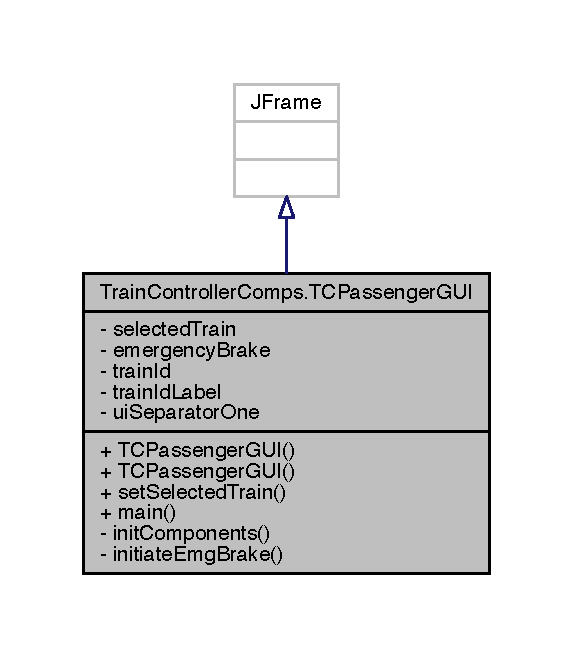
\includegraphics[width=275pt]{classTrainControllerComps_1_1TCPassengerGUI__inherit__graph}
\end{center}
\end{figure}


Collaboration diagram for Train\+Controller\+Comps.\+T\+C\+Passenger\+G\+UI\+:
\nopagebreak
\begin{figure}[H]
\begin{center}
\leavevmode
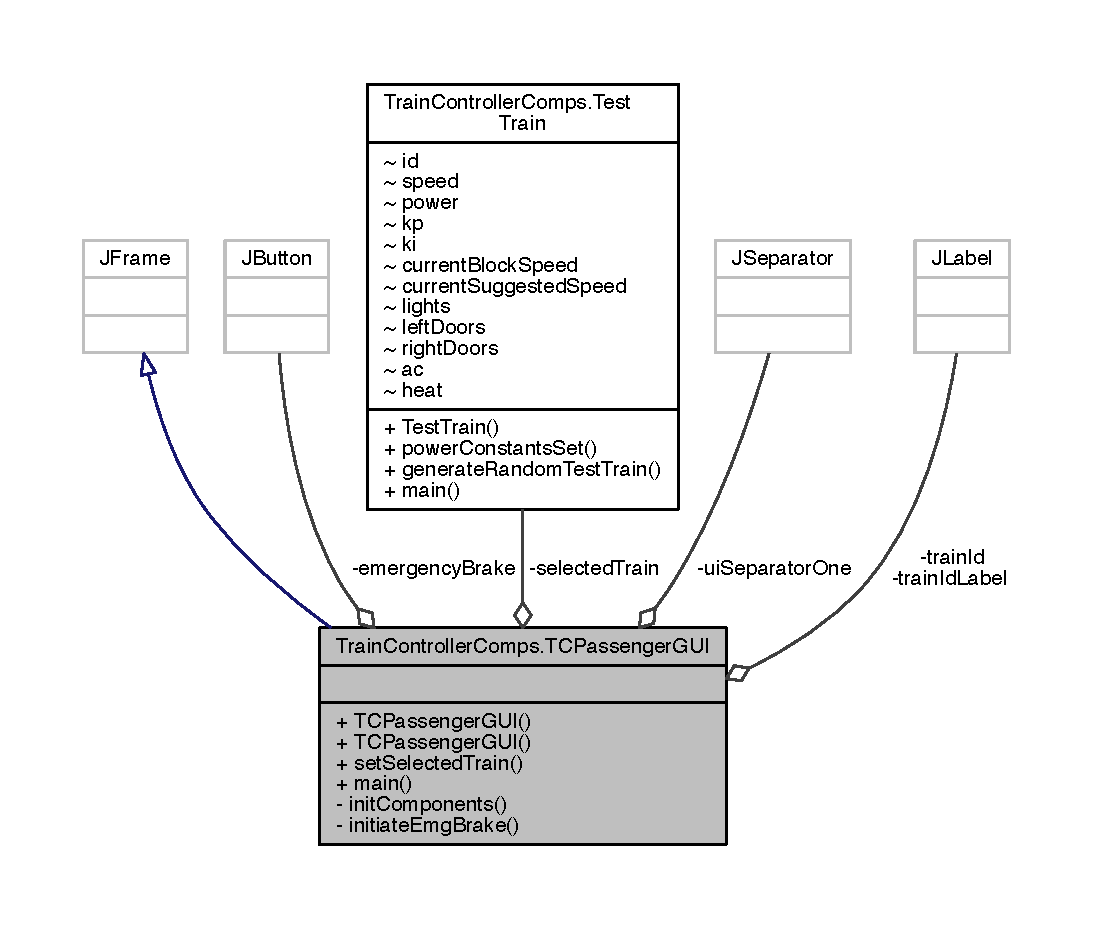
\includegraphics[width=350pt]{classTrainControllerComps_1_1TCPassengerGUI__coll__graph}
\end{center}
\end{figure}
\subsection*{Public Member Functions}
\begin{DoxyCompactItemize}
\item 
\hyperlink{classTrainControllerComps_1_1TCPassengerGUI_a87ff0e93bee02d188abdd03e33517244}{T\+C\+Passenger\+G\+UI} ()
\begin{DoxyCompactList}\small\item\em Constructor for creating a \hyperlink{classTrainControllerComps_1_1TCPassengerGUI}{T\+C\+Passenger\+G\+UI} object with no selected train. \end{DoxyCompactList}\item 
\hyperlink{classTrainControllerComps_1_1TCPassengerGUI_a1a4a77c620d2c30d15de7d18068893f1}{T\+C\+Passenger\+G\+UI} (\hyperlink{classTrainControllerComps_1_1TestTrain}{Test\+Train} \hyperlink{classtrain}{train})
\begin{DoxyCompactList}\small\item\em Constructor for creating a \hyperlink{classTrainControllerComps_1_1TCPassengerGUI}{T\+C\+Passenger\+G\+UI} object with a selected train. \end{DoxyCompactList}\item 
void \hyperlink{classTrainControllerComps_1_1TCPassengerGUI_ac6b3f1baa4e1d4856020854281786cf8}{set\+Selected\+Train} (\hyperlink{classTrainControllerComps_1_1TestTrain}{Test\+Train} \hyperlink{classtrain}{train})
\end{DoxyCompactItemize}
\subsection*{Static Public Member Functions}
\begin{DoxyCompactItemize}
\item 
static void \hyperlink{classTrainControllerComps_1_1TCPassengerGUI_a65b80b653964f7bd6822a424c78b1a54}{main} (String args\mbox{[}$\,$\mbox{]})
\end{DoxyCompactItemize}
\subsection*{Private Member Functions}
\begin{DoxyCompactItemize}
\item 
void \hyperlink{classTrainControllerComps_1_1TCPassengerGUI_a0470c9528fe420297061ed084b92e7c4}{init\+Components} ()
\begin{DoxyCompactList}\small\item\em This method is called from within the constructor to initialize the form. \end{DoxyCompactList}\item 
void \hyperlink{classTrainControllerComps_1_1TCPassengerGUI_a41e6c77f96e89bb0b247668cc426f522}{initiate\+Emg\+Brake} (java.\+awt.\+event.\+Action\+Event evt)
\begin{DoxyCompactList}\small\item\em Initiates the emergency brake on the selected train. \end{DoxyCompactList}\end{DoxyCompactItemize}
\subsection*{Private Attributes}
\begin{DoxyCompactItemize}
\item 
\hyperlink{classTrainControllerComps_1_1TestTrain}{Test\+Train} \hyperlink{classTrainControllerComps_1_1TCPassengerGUI_afcf53b411242f019ef96ef8e593f5b6a}{selected\+Train}
\begin{DoxyCompactList}\small\item\em The train being controlled by the Train Controller. \end{DoxyCompactList}\item 
javax.\+swing.\+J\+Button \hyperlink{classTrainControllerComps_1_1TCPassengerGUI_a45d3019b50112c727dbd12233ba3a822}{emergency\+Brake}
\item 
javax.\+swing.\+J\+Label \hyperlink{classTrainControllerComps_1_1TCPassengerGUI_a986818d54895ef1956c5ee655e3c7637}{train\+Id}
\item 
javax.\+swing.\+J\+Label \hyperlink{classTrainControllerComps_1_1TCPassengerGUI_ad919d2752a791d156963ddff49886595}{train\+Id\+Label}
\item 
javax.\+swing.\+J\+Separator \hyperlink{classTrainControllerComps_1_1TCPassengerGUI_ac8aa2c896b5f794013cedb4c3f07c5b3}{ui\+Separator\+One}
\end{DoxyCompactItemize}


\subsection{Detailed Description}
This class is responsible for allowing the passengers on the train to initiate the emergency brake on a selected train. 

This class collaborates with the Train Controller and Train class.

\begin{DoxyAuthor}{Author}
Andrew Lendacky 
\end{DoxyAuthor}


\subsection{Constructor \& Destructor Documentation}
\mbox{\Hypertarget{classTrainControllerComps_1_1TCPassengerGUI_a87ff0e93bee02d188abdd03e33517244}\label{classTrainControllerComps_1_1TCPassengerGUI_a87ff0e93bee02d188abdd03e33517244}} 
\index{Train\+Controller\+Comps\+::\+T\+C\+Passenger\+G\+UI@{Train\+Controller\+Comps\+::\+T\+C\+Passenger\+G\+UI}!T\+C\+Passenger\+G\+UI@{T\+C\+Passenger\+G\+UI}}
\index{T\+C\+Passenger\+G\+UI@{T\+C\+Passenger\+G\+UI}!Train\+Controller\+Comps\+::\+T\+C\+Passenger\+G\+UI@{Train\+Controller\+Comps\+::\+T\+C\+Passenger\+G\+UI}}
\subsubsection{\texorpdfstring{T\+C\+Passenger\+G\+U\+I()}{TCPassengerGUI()}\hspace{0.1cm}{\footnotesize\ttfamily [1/2]}}
{\footnotesize\ttfamily Train\+Controller\+Comps.\+T\+C\+Passenger\+G\+U\+I.\+T\+C\+Passenger\+G\+UI (\begin{DoxyParamCaption}{ }\end{DoxyParamCaption})}



Constructor for creating a \hyperlink{classTrainControllerComps_1_1TCPassengerGUI}{T\+C\+Passenger\+G\+UI} object with no selected train. 

The selected train must be set by the Train Controller before being used. \mbox{\Hypertarget{classTrainControllerComps_1_1TCPassengerGUI_a1a4a77c620d2c30d15de7d18068893f1}\label{classTrainControllerComps_1_1TCPassengerGUI_a1a4a77c620d2c30d15de7d18068893f1}} 
\index{Train\+Controller\+Comps\+::\+T\+C\+Passenger\+G\+UI@{Train\+Controller\+Comps\+::\+T\+C\+Passenger\+G\+UI}!T\+C\+Passenger\+G\+UI@{T\+C\+Passenger\+G\+UI}}
\index{T\+C\+Passenger\+G\+UI@{T\+C\+Passenger\+G\+UI}!Train\+Controller\+Comps\+::\+T\+C\+Passenger\+G\+UI@{Train\+Controller\+Comps\+::\+T\+C\+Passenger\+G\+UI}}
\subsubsection{\texorpdfstring{T\+C\+Passenger\+G\+U\+I()}{TCPassengerGUI()}\hspace{0.1cm}{\footnotesize\ttfamily [2/2]}}
{\footnotesize\ttfamily Train\+Controller\+Comps.\+T\+C\+Passenger\+G\+U\+I.\+T\+C\+Passenger\+G\+UI (\begin{DoxyParamCaption}\item[{\hyperlink{classTrainControllerComps_1_1TestTrain}{Test\+Train}}]{train }\end{DoxyParamCaption})}



Constructor for creating a \hyperlink{classTrainControllerComps_1_1TCPassengerGUI}{T\+C\+Passenger\+G\+UI} object with a selected train. 


\begin{DoxyParams}{Parameters}
{\em train} & the train controlled by the Train Controller class. \\
\hline
\end{DoxyParams}


\subsection{Member Function Documentation}
\mbox{\Hypertarget{classTrainControllerComps_1_1TCPassengerGUI_a0470c9528fe420297061ed084b92e7c4}\label{classTrainControllerComps_1_1TCPassengerGUI_a0470c9528fe420297061ed084b92e7c4}} 
\index{Train\+Controller\+Comps\+::\+T\+C\+Passenger\+G\+UI@{Train\+Controller\+Comps\+::\+T\+C\+Passenger\+G\+UI}!init\+Components@{init\+Components}}
\index{init\+Components@{init\+Components}!Train\+Controller\+Comps\+::\+T\+C\+Passenger\+G\+UI@{Train\+Controller\+Comps\+::\+T\+C\+Passenger\+G\+UI}}
\subsubsection{\texorpdfstring{init\+Components()}{initComponents()}}
{\footnotesize\ttfamily void Train\+Controller\+Comps.\+T\+C\+Passenger\+G\+U\+I.\+init\+Components (\begin{DoxyParamCaption}{ }\end{DoxyParamCaption})\hspace{0.3cm}{\ttfamily [private]}}



This method is called from within the constructor to initialize the form. 

W\+A\+R\+N\+I\+NG\+: Do N\+OT modify this code. The content of this method is always regenerated by the Form Editor. \mbox{\Hypertarget{classTrainControllerComps_1_1TCPassengerGUI_a41e6c77f96e89bb0b247668cc426f522}\label{classTrainControllerComps_1_1TCPassengerGUI_a41e6c77f96e89bb0b247668cc426f522}} 
\index{Train\+Controller\+Comps\+::\+T\+C\+Passenger\+G\+UI@{Train\+Controller\+Comps\+::\+T\+C\+Passenger\+G\+UI}!initiate\+Emg\+Brake@{initiate\+Emg\+Brake}}
\index{initiate\+Emg\+Brake@{initiate\+Emg\+Brake}!Train\+Controller\+Comps\+::\+T\+C\+Passenger\+G\+UI@{Train\+Controller\+Comps\+::\+T\+C\+Passenger\+G\+UI}}
\subsubsection{\texorpdfstring{initiate\+Emg\+Brake()}{initiateEmgBrake()}}
{\footnotesize\ttfamily void Train\+Controller\+Comps.\+T\+C\+Passenger\+G\+U\+I.\+initiate\+Emg\+Brake (\begin{DoxyParamCaption}\item[{java.\+awt.\+event.\+Action\+Event}]{evt }\end{DoxyParamCaption})\hspace{0.3cm}{\ttfamily [private]}}



Initiates the emergency brake on the selected train. 


\begin{DoxyParams}{Parameters}
{\em evt} & the sender of the event, i.\+e., the \textquotesingle{}Emergency Brake\textquotesingle{} button \\
\hline
\end{DoxyParams}
\mbox{\Hypertarget{classTrainControllerComps_1_1TCPassengerGUI_a65b80b653964f7bd6822a424c78b1a54}\label{classTrainControllerComps_1_1TCPassengerGUI_a65b80b653964f7bd6822a424c78b1a54}} 
\index{Train\+Controller\+Comps\+::\+T\+C\+Passenger\+G\+UI@{Train\+Controller\+Comps\+::\+T\+C\+Passenger\+G\+UI}!main@{main}}
\index{main@{main}!Train\+Controller\+Comps\+::\+T\+C\+Passenger\+G\+UI@{Train\+Controller\+Comps\+::\+T\+C\+Passenger\+G\+UI}}
\subsubsection{\texorpdfstring{main()}{main()}}
{\footnotesize\ttfamily static void Train\+Controller\+Comps.\+T\+C\+Passenger\+G\+U\+I.\+main (\begin{DoxyParamCaption}\item[{String}]{args\mbox{[}$\,$\mbox{]} }\end{DoxyParamCaption})\hspace{0.3cm}{\ttfamily [static]}}


\begin{DoxyParams}{Parameters}
{\em args} & the command line arguments \\
\hline
\end{DoxyParams}
\mbox{\Hypertarget{classTrainControllerComps_1_1TCPassengerGUI_ac6b3f1baa4e1d4856020854281786cf8}\label{classTrainControllerComps_1_1TCPassengerGUI_ac6b3f1baa4e1d4856020854281786cf8}} 
\index{Train\+Controller\+Comps\+::\+T\+C\+Passenger\+G\+UI@{Train\+Controller\+Comps\+::\+T\+C\+Passenger\+G\+UI}!set\+Selected\+Train@{set\+Selected\+Train}}
\index{set\+Selected\+Train@{set\+Selected\+Train}!Train\+Controller\+Comps\+::\+T\+C\+Passenger\+G\+UI@{Train\+Controller\+Comps\+::\+T\+C\+Passenger\+G\+UI}}
\subsubsection{\texorpdfstring{set\+Selected\+Train()}{setSelectedTrain()}}
{\footnotesize\ttfamily void Train\+Controller\+Comps.\+T\+C\+Passenger\+G\+U\+I.\+set\+Selected\+Train (\begin{DoxyParamCaption}\item[{\hyperlink{classTrainControllerComps_1_1TestTrain}{Test\+Train}}]{train }\end{DoxyParamCaption})}



\subsection{Member Data Documentation}
\mbox{\Hypertarget{classTrainControllerComps_1_1TCPassengerGUI_a45d3019b50112c727dbd12233ba3a822}\label{classTrainControllerComps_1_1TCPassengerGUI_a45d3019b50112c727dbd12233ba3a822}} 
\index{Train\+Controller\+Comps\+::\+T\+C\+Passenger\+G\+UI@{Train\+Controller\+Comps\+::\+T\+C\+Passenger\+G\+UI}!emergency\+Brake@{emergency\+Brake}}
\index{emergency\+Brake@{emergency\+Brake}!Train\+Controller\+Comps\+::\+T\+C\+Passenger\+G\+UI@{Train\+Controller\+Comps\+::\+T\+C\+Passenger\+G\+UI}}
\subsubsection{\texorpdfstring{emergency\+Brake}{emergencyBrake}}
{\footnotesize\ttfamily javax.\+swing.\+J\+Button Train\+Controller\+Comps.\+T\+C\+Passenger\+G\+U\+I.\+emergency\+Brake\hspace{0.3cm}{\ttfamily [private]}}

\mbox{\Hypertarget{classTrainControllerComps_1_1TCPassengerGUI_afcf53b411242f019ef96ef8e593f5b6a}\label{classTrainControllerComps_1_1TCPassengerGUI_afcf53b411242f019ef96ef8e593f5b6a}} 
\index{Train\+Controller\+Comps\+::\+T\+C\+Passenger\+G\+UI@{Train\+Controller\+Comps\+::\+T\+C\+Passenger\+G\+UI}!selected\+Train@{selected\+Train}}
\index{selected\+Train@{selected\+Train}!Train\+Controller\+Comps\+::\+T\+C\+Passenger\+G\+UI@{Train\+Controller\+Comps\+::\+T\+C\+Passenger\+G\+UI}}
\subsubsection{\texorpdfstring{selected\+Train}{selectedTrain}}
{\footnotesize\ttfamily \hyperlink{classTrainControllerComps_1_1TestTrain}{Test\+Train} Train\+Controller\+Comps.\+T\+C\+Passenger\+G\+U\+I.\+selected\+Train\hspace{0.3cm}{\ttfamily [private]}}



The train being controlled by the Train Controller. 

\mbox{\Hypertarget{classTrainControllerComps_1_1TCPassengerGUI_a986818d54895ef1956c5ee655e3c7637}\label{classTrainControllerComps_1_1TCPassengerGUI_a986818d54895ef1956c5ee655e3c7637}} 
\index{Train\+Controller\+Comps\+::\+T\+C\+Passenger\+G\+UI@{Train\+Controller\+Comps\+::\+T\+C\+Passenger\+G\+UI}!train\+Id@{train\+Id}}
\index{train\+Id@{train\+Id}!Train\+Controller\+Comps\+::\+T\+C\+Passenger\+G\+UI@{Train\+Controller\+Comps\+::\+T\+C\+Passenger\+G\+UI}}
\subsubsection{\texorpdfstring{train\+Id}{trainId}}
{\footnotesize\ttfamily javax.\+swing.\+J\+Label Train\+Controller\+Comps.\+T\+C\+Passenger\+G\+U\+I.\+train\+Id\hspace{0.3cm}{\ttfamily [private]}}

\mbox{\Hypertarget{classTrainControllerComps_1_1TCPassengerGUI_ad919d2752a791d156963ddff49886595}\label{classTrainControllerComps_1_1TCPassengerGUI_ad919d2752a791d156963ddff49886595}} 
\index{Train\+Controller\+Comps\+::\+T\+C\+Passenger\+G\+UI@{Train\+Controller\+Comps\+::\+T\+C\+Passenger\+G\+UI}!train\+Id\+Label@{train\+Id\+Label}}
\index{train\+Id\+Label@{train\+Id\+Label}!Train\+Controller\+Comps\+::\+T\+C\+Passenger\+G\+UI@{Train\+Controller\+Comps\+::\+T\+C\+Passenger\+G\+UI}}
\subsubsection{\texorpdfstring{train\+Id\+Label}{trainIdLabel}}
{\footnotesize\ttfamily javax.\+swing.\+J\+Label Train\+Controller\+Comps.\+T\+C\+Passenger\+G\+U\+I.\+train\+Id\+Label\hspace{0.3cm}{\ttfamily [private]}}

\mbox{\Hypertarget{classTrainControllerComps_1_1TCPassengerGUI_ac8aa2c896b5f794013cedb4c3f07c5b3}\label{classTrainControllerComps_1_1TCPassengerGUI_ac8aa2c896b5f794013cedb4c3f07c5b3}} 
\index{Train\+Controller\+Comps\+::\+T\+C\+Passenger\+G\+UI@{Train\+Controller\+Comps\+::\+T\+C\+Passenger\+G\+UI}!ui\+Separator\+One@{ui\+Separator\+One}}
\index{ui\+Separator\+One@{ui\+Separator\+One}!Train\+Controller\+Comps\+::\+T\+C\+Passenger\+G\+UI@{Train\+Controller\+Comps\+::\+T\+C\+Passenger\+G\+UI}}
\subsubsection{\texorpdfstring{ui\+Separator\+One}{uiSeparatorOne}}
{\footnotesize\ttfamily javax.\+swing.\+J\+Separator Train\+Controller\+Comps.\+T\+C\+Passenger\+G\+U\+I.\+ui\+Separator\+One\hspace{0.3cm}{\ttfamily [private]}}



The documentation for this class was generated from the following file\+:\begin{DoxyCompactItemize}
\item 
src/main/java/\+Train\+Controller\+Comps/\hyperlink{TCPassengerGUI_8java}{T\+C\+Passenger\+G\+U\+I.\+java}\end{DoxyCompactItemize}

\hypertarget{classTrainControllerComps_1_1TCSpeedController}{}\section{Train\+Controller\+Comps.\+T\+C\+Speed\+Controller Class Reference}
\label{classTrainControllerComps_1_1TCSpeedController}\index{Train\+Controller\+Comps.\+T\+C\+Speed\+Controller@{Train\+Controller\+Comps.\+T\+C\+Speed\+Controller}}


This class is responsible for allowing the user to set the speed of the selected train if in Manual mode, or controls the speed automatically if in Automatic mode.  




Inheritance diagram for Train\+Controller\+Comps.\+T\+C\+Speed\+Controller\+:
\nopagebreak
\begin{figure}[H]
\begin{center}
\leavevmode
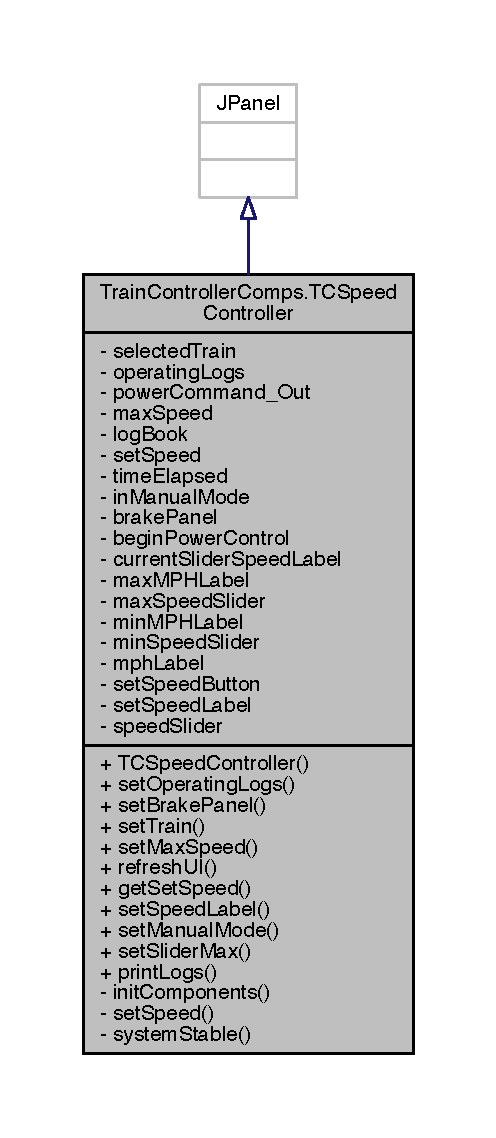
\includegraphics[width=238pt]{classTrainControllerComps_1_1TCSpeedController__inherit__graph}
\end{center}
\end{figure}


Collaboration diagram for Train\+Controller\+Comps.\+T\+C\+Speed\+Controller\+:
\nopagebreak
\begin{figure}[H]
\begin{center}
\leavevmode
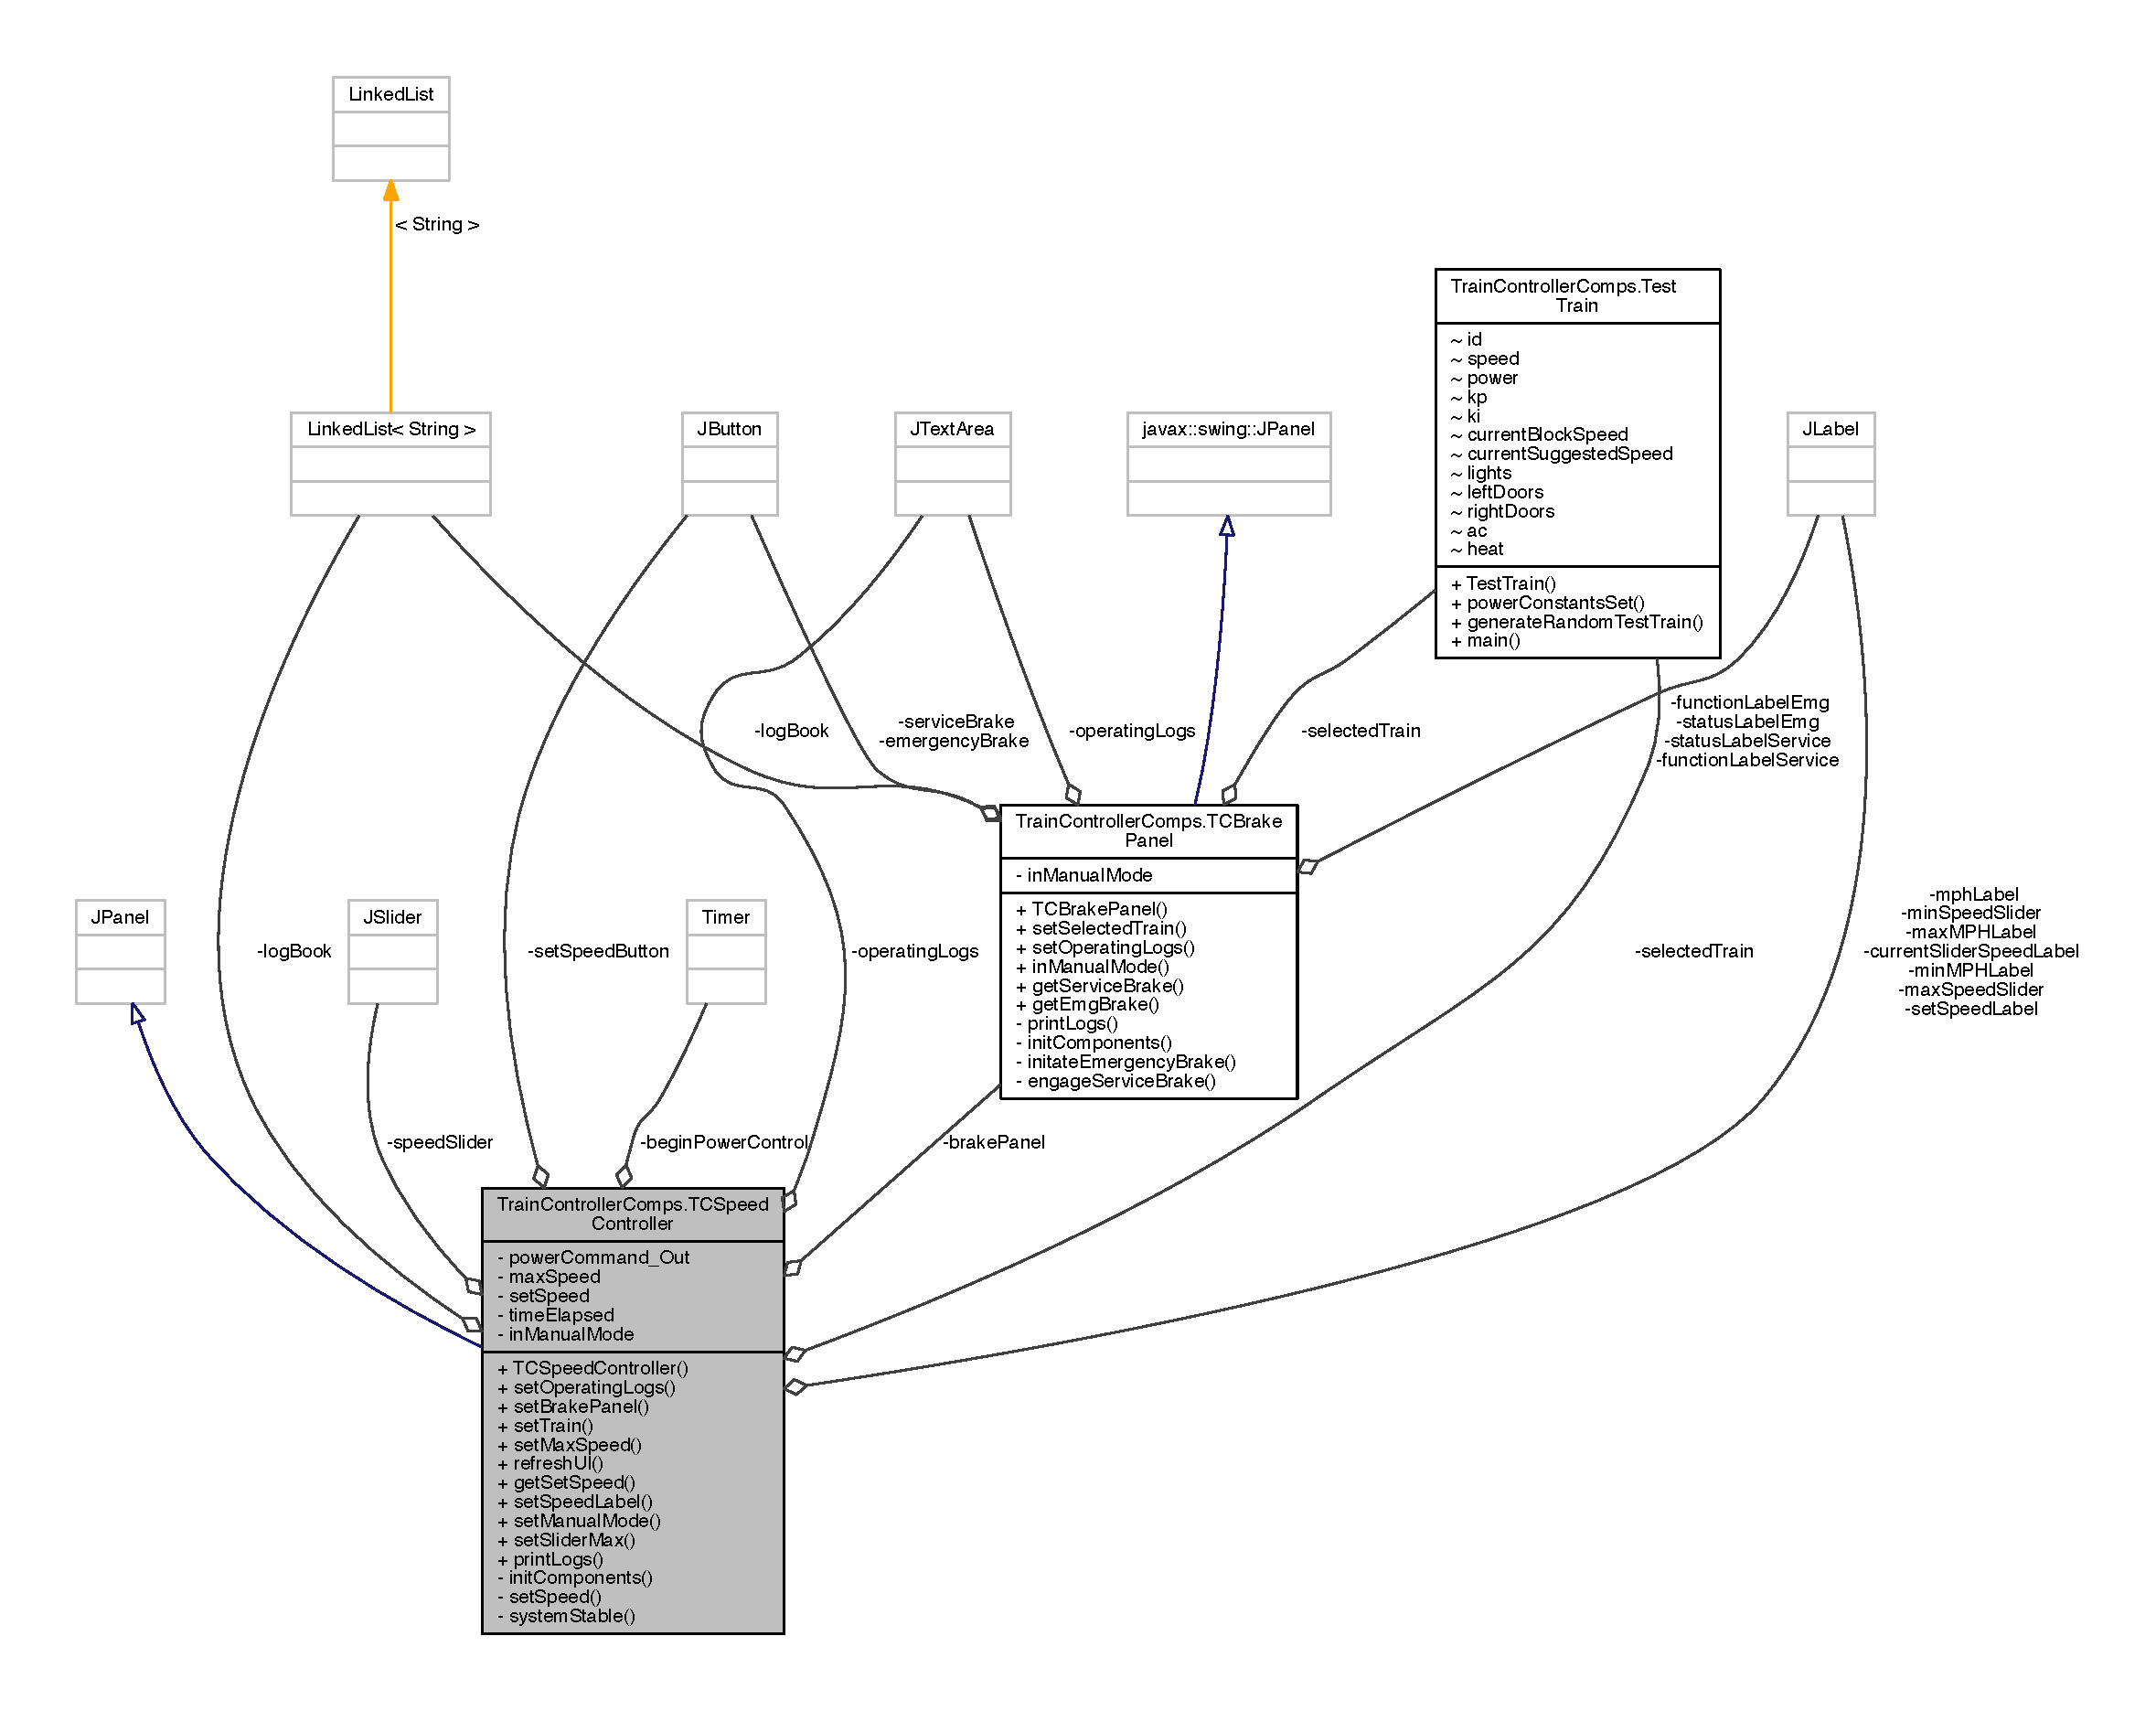
\includegraphics[width=350pt]{classTrainControllerComps_1_1TCSpeedController__coll__graph}
\end{center}
\end{figure}
\subsection*{Public Member Functions}
\begin{DoxyCompactItemize}
\item 
\hyperlink{classTrainControllerComps_1_1TCSpeedController_a2bf8141c881ab8a26b084813be33a200}{T\+C\+Speed\+Controller} ()
\begin{DoxyCompactList}\small\item\em Constructor for creating a new \hyperlink{classTrainControllerComps_1_1TCSpeedController}{T\+C\+Speed\+Controller} object with no selected train. \end{DoxyCompactList}\item 
void \hyperlink{classTrainControllerComps_1_1TCSpeedController_aa77cc92612065fb35630dc957e51d131}{set\+Operating\+Logs} (J\+Text\+Area op\+Logs)
\begin{DoxyCompactList}\small\item\em Sets which Operating Logs the Speed Controller should print to. \end{DoxyCompactList}\item 
void \hyperlink{classTrainControllerComps_1_1TCSpeedController_a986d53f2a607902b98706f9cde8d80b0}{set\+Brake\+Panel} (\hyperlink{classTrainControllerComps_1_1TCBrakePanel}{T\+C\+Brake\+Panel} \hyperlink{classTrainControllerComps_1_1TCSpeedController_a539321041f3ef8431e32bd9fa9238541}{brake\+Panel})
\begin{DoxyCompactList}\small\item\em Sets the brake panel. \end{DoxyCompactList}\item 
void \hyperlink{classTrainControllerComps_1_1TCSpeedController_a5f707ae153cba07e276eab9c7fff7136}{set\+Train} (\hyperlink{classTrainControllerComps_1_1TestTrain}{Test\+Train} \hyperlink{classtrain}{train})
\begin{DoxyCompactList}\small\item\em Gives the Speed Controller the train whose speed to it has to change. \end{DoxyCompactList}\item 
void \hyperlink{classTrainControllerComps_1_1TCSpeedController_aacfc193db3b550fe02839a55152573cb}{set\+Max\+Speed} (double \hyperlink{classTrainControllerComps_1_1TCSpeedController_abd22aed945ca95e2bd476cf9cc2abcbd}{max\+Speed})
\begin{DoxyCompactList}\small\item\em Sets the max speed the train is allowed to go, and then updates the UI so that the slider\textquotesingle{}s max value is that of the max\+Speed and the correct speed is on the label. \end{DoxyCompactList}\item 
void \hyperlink{classTrainControllerComps_1_1TCSpeedController_a037818d87276a705484f59c19cdbfa6f}{refresh\+UI} ()
\begin{DoxyCompactList}\small\item\em Refreshes all the UI components in the Speed\+Controller. \end{DoxyCompactList}\item 
int \hyperlink{classTrainControllerComps_1_1TCSpeedController_a46ca9df1d707cecd4167a532babcf6ed}{get\+Set\+Speed} ()
\begin{DoxyCompactList}\small\item\em Retrieves the set speed the user wants the train to go, which is determined by the speed slider. \end{DoxyCompactList}\item 
void \hyperlink{classTrainControllerComps_1_1TCSpeedController_afef25cbf49579c1ac17414ba29b30c13}{set\+Speed\+Label} ()
\begin{DoxyCompactList}\small\item\em Updates the speed label with that of the slider value. \end{DoxyCompactList}\item 
void \hyperlink{classTrainControllerComps_1_1TCSpeedController_a029c45976f5b311e30f90562acecbf8e}{set\+Manual\+Mode} (Boolean b)
\begin{DoxyCompactList}\small\item\em Sets if the Speed Controller should run in Manual or Automatic mode. \end{DoxyCompactList}\item 
void \hyperlink{classTrainControllerComps_1_1TCSpeedController_a1373bc000dd8c13b47d9a298c383dd7e}{set\+Slider\+Max} (int max)
\begin{DoxyCompactList}\small\item\em Sets the max value of the speed controller slider. \end{DoxyCompactList}\item 
void \hyperlink{classTrainControllerComps_1_1TCSpeedController_a0aff8debe964e2c66d38a065052bbb2a}{print\+Logs} ()
\begin{DoxyCompactList}\small\item\em Prints the stored logs to the operating log, then clears the logbook. \end{DoxyCompactList}\end{DoxyCompactItemize}
\subsection*{Private Member Functions}
\begin{DoxyCompactItemize}
\item 
void \hyperlink{classTrainControllerComps_1_1TCSpeedController_a2b6b810eeb4e36a5932b6c26babfd7a2}{init\+Components} ()
\begin{DoxyCompactList}\small\item\em This method is called from within the constructor to initialize the form. \end{DoxyCompactList}\item 
void \hyperlink{classTrainControllerComps_1_1TCSpeedController_a85b0846fba0d3db24f1719437ad854d9}{set\+Speed} (java.\+awt.\+event.\+Action\+Event evt)
\begin{DoxyCompactList}\small\item\em Begins the process of changing the selected train\textquotesingle{}s speed by using Power Control Law. \end{DoxyCompactList}\item 
boolean \hyperlink{classTrainControllerComps_1_1TCSpeedController_a1a67c88e2bbc9543cfe1a910c7cab35f}{system\+Stable} ()
\begin{DoxyCompactList}\small\item\em Determines if the the train\textquotesingle{}s speed is equal to the speed the user set. \end{DoxyCompactList}\end{DoxyCompactItemize}
\subsection*{Private Attributes}
\begin{DoxyCompactItemize}
\item 
\hyperlink{classTrainControllerComps_1_1TestTrain}{Test\+Train} \hyperlink{classTrainControllerComps_1_1TCSpeedController_ab8484141d0674b98f2b6d512dd190f5a}{selected\+Train}
\begin{DoxyCompactList}\small\item\em The train that is being controlled by the Train Controller. \end{DoxyCompactList}\item 
J\+Text\+Area \hyperlink{classTrainControllerComps_1_1TCSpeedController_a0cb92a0d707d38f6c2d82a40bb4dd853}{operating\+Logs}
\begin{DoxyCompactList}\small\item\em Area the logs are printed to. \end{DoxyCompactList}\item 
double \hyperlink{classTrainControllerComps_1_1TCSpeedController_a3ed394303d0d4f4c947dc2abcc6f18d3}{power\+Command\+\_\+\+Out}
\begin{DoxyCompactList}\small\item\em This is the power command sent from the Train Controller to the train. \end{DoxyCompactList}\item 
double \hyperlink{classTrainControllerComps_1_1TCSpeedController_abd22aed945ca95e2bd476cf9cc2abcbd}{max\+Speed}
\begin{DoxyCompactList}\small\item\em Max speed the train is allowed to go. \end{DoxyCompactList}\item 
Linked\+List$<$ String $>$ \hyperlink{classTrainControllerComps_1_1TCSpeedController_a1a4a076e7c917a5ddfe19d80b29cff62}{log\+Book}
\begin{DoxyCompactList}\small\item\em A list that is used to hold logs to print to the Operating Logs of the Train Controller. \end{DoxyCompactList}\item 
int \hyperlink{classTrainControllerComps_1_1TCSpeedController_a68f33f6aaf56d44c66e21b1acfe92ff4}{set\+Speed}
\begin{DoxyCompactList}\small\item\em The speed that the train is desired to go. \end{DoxyCompactList}\item 
int \hyperlink{classTrainControllerComps_1_1TCSpeedController_aa94c86762d0a9c73b32be1165d78b436}{time\+Elapsed}
\begin{DoxyCompactList}\small\item\em Used to keep track of how long it takes the train to reach the set speed. \end{DoxyCompactList}\item 
boolean \hyperlink{classTrainControllerComps_1_1TCSpeedController_a00ba0c34f85995b6c0f6d440f9661b22}{in\+Manual\+Mode}
\begin{DoxyCompactList}\small\item\em A boolean value indicating if the Speed Controller is operating in Manual or Automatic mode. \end{DoxyCompactList}\item 
\hyperlink{classTrainControllerComps_1_1TCBrakePanel}{T\+C\+Brake\+Panel} \hyperlink{classTrainControllerComps_1_1TCSpeedController_a539321041f3ef8431e32bd9fa9238541}{brake\+Panel}
\begin{DoxyCompactList}\small\item\em Brake panel used to control the brakes on the train if needed to slow down. \end{DoxyCompactList}\item 
Timer \hyperlink{classTrainControllerComps_1_1TCSpeedController_aa0bbb3afbc3ce25274a258dc7561df1e}{begin\+Power\+Control}
\begin{DoxyCompactList}\small\item\em Timer used to perform the power law calculations with the train 1 second. \end{DoxyCompactList}\item 
javax.\+swing.\+J\+Label \hyperlink{classTrainControllerComps_1_1TCSpeedController_aa8e5481a7f4ef453cbe6d1d3768657b7}{current\+Slider\+Speed\+Label}
\item 
javax.\+swing.\+J\+Label \hyperlink{classTrainControllerComps_1_1TCSpeedController_af060c649756f16edd6e2100629e2445d}{max\+M\+P\+H\+Label}
\item 
javax.\+swing.\+J\+Label \hyperlink{classTrainControllerComps_1_1TCSpeedController_a637084d67743ab5a28f41f02eaa5167c}{max\+Speed\+Slider}
\item 
javax.\+swing.\+J\+Label \hyperlink{classTrainControllerComps_1_1TCSpeedController_acf758cad7ad3d1f29392d8fab7a2312c}{min\+M\+P\+H\+Label}
\item 
javax.\+swing.\+J\+Label \hyperlink{classTrainControllerComps_1_1TCSpeedController_a2d1579eee22df41f38253c5cb07380a8}{min\+Speed\+Slider}
\item 
javax.\+swing.\+J\+Label \hyperlink{classTrainControllerComps_1_1TCSpeedController_a681d1c2c9079a1207d4360cf37da07af}{mph\+Label}
\item 
javax.\+swing.\+J\+Button \hyperlink{classTrainControllerComps_1_1TCSpeedController_ab120f3835e3e8c45f84377cdd92f35c1}{set\+Speed\+Button}
\item 
javax.\+swing.\+J\+Label \hyperlink{classTrainControllerComps_1_1TCSpeedController_ad089c32c9a1548349c55c3468a97848d}{set\+Speed\+Label}
\item 
javax.\+swing.\+J\+Slider \hyperlink{classTrainControllerComps_1_1TCSpeedController_ac4869ca6b35dbfb1c44385205c2d13c5}{speed\+Slider}
\end{DoxyCompactItemize}


\subsection{Detailed Description}
This class is responsible for allowing the user to set the speed of the selected train if in Manual mode, or controls the speed automatically if in Automatic mode. 

This class collaborates with the Train and Train Controller class.

\begin{DoxyAuthor}{Author}
Andrew Lendacky 
\end{DoxyAuthor}


\subsection{Constructor \& Destructor Documentation}
\mbox{\Hypertarget{classTrainControllerComps_1_1TCSpeedController_a2bf8141c881ab8a26b084813be33a200}\label{classTrainControllerComps_1_1TCSpeedController_a2bf8141c881ab8a26b084813be33a200}} 
\index{Train\+Controller\+Comps\+::\+T\+C\+Speed\+Controller@{Train\+Controller\+Comps\+::\+T\+C\+Speed\+Controller}!T\+C\+Speed\+Controller@{T\+C\+Speed\+Controller}}
\index{T\+C\+Speed\+Controller@{T\+C\+Speed\+Controller}!Train\+Controller\+Comps\+::\+T\+C\+Speed\+Controller@{Train\+Controller\+Comps\+::\+T\+C\+Speed\+Controller}}
\subsubsection{\texorpdfstring{T\+C\+Speed\+Controller()}{TCSpeedController()}}
{\footnotesize\ttfamily Train\+Controller\+Comps.\+T\+C\+Speed\+Controller.\+T\+C\+Speed\+Controller (\begin{DoxyParamCaption}{ }\end{DoxyParamCaption})}



Constructor for creating a new \hyperlink{classTrainControllerComps_1_1TCSpeedController}{T\+C\+Speed\+Controller} object with no selected train. 

The selected train must be set by the Train Controller before being used. 

\subsection{Member Function Documentation}
\mbox{\Hypertarget{classTrainControllerComps_1_1TCSpeedController_a46ca9df1d707cecd4167a532babcf6ed}\label{classTrainControllerComps_1_1TCSpeedController_a46ca9df1d707cecd4167a532babcf6ed}} 
\index{Train\+Controller\+Comps\+::\+T\+C\+Speed\+Controller@{Train\+Controller\+Comps\+::\+T\+C\+Speed\+Controller}!get\+Set\+Speed@{get\+Set\+Speed}}
\index{get\+Set\+Speed@{get\+Set\+Speed}!Train\+Controller\+Comps\+::\+T\+C\+Speed\+Controller@{Train\+Controller\+Comps\+::\+T\+C\+Speed\+Controller}}
\subsubsection{\texorpdfstring{get\+Set\+Speed()}{getSetSpeed()}}
{\footnotesize\ttfamily int Train\+Controller\+Comps.\+T\+C\+Speed\+Controller.\+get\+Set\+Speed (\begin{DoxyParamCaption}{ }\end{DoxyParamCaption})}



Retrieves the set speed the user wants the train to go, which is determined by the speed slider. 

\begin{DoxyReturn}{Returns}
returns the value of the speed slider. 
\end{DoxyReturn}
\mbox{\Hypertarget{classTrainControllerComps_1_1TCSpeedController_a2b6b810eeb4e36a5932b6c26babfd7a2}\label{classTrainControllerComps_1_1TCSpeedController_a2b6b810eeb4e36a5932b6c26babfd7a2}} 
\index{Train\+Controller\+Comps\+::\+T\+C\+Speed\+Controller@{Train\+Controller\+Comps\+::\+T\+C\+Speed\+Controller}!init\+Components@{init\+Components}}
\index{init\+Components@{init\+Components}!Train\+Controller\+Comps\+::\+T\+C\+Speed\+Controller@{Train\+Controller\+Comps\+::\+T\+C\+Speed\+Controller}}
\subsubsection{\texorpdfstring{init\+Components()}{initComponents()}}
{\footnotesize\ttfamily void Train\+Controller\+Comps.\+T\+C\+Speed\+Controller.\+init\+Components (\begin{DoxyParamCaption}{ }\end{DoxyParamCaption})\hspace{0.3cm}{\ttfamily [private]}}



This method is called from within the constructor to initialize the form. 

W\+A\+R\+N\+I\+NG\+: Do N\+OT modify this code. The content of this method is always regenerated by the Form Editor. \mbox{\Hypertarget{classTrainControllerComps_1_1TCSpeedController_a0aff8debe964e2c66d38a065052bbb2a}\label{classTrainControllerComps_1_1TCSpeedController_a0aff8debe964e2c66d38a065052bbb2a}} 
\index{Train\+Controller\+Comps\+::\+T\+C\+Speed\+Controller@{Train\+Controller\+Comps\+::\+T\+C\+Speed\+Controller}!print\+Logs@{print\+Logs}}
\index{print\+Logs@{print\+Logs}!Train\+Controller\+Comps\+::\+T\+C\+Speed\+Controller@{Train\+Controller\+Comps\+::\+T\+C\+Speed\+Controller}}
\subsubsection{\texorpdfstring{print\+Logs()}{printLogs()}}
{\footnotesize\ttfamily void Train\+Controller\+Comps.\+T\+C\+Speed\+Controller.\+print\+Logs (\begin{DoxyParamCaption}{ }\end{DoxyParamCaption})}



Prints the stored logs to the operating log, then clears the logbook. 

The J\+Text\+Pane must be set from the \hyperlink{classTrainControllerComps_1_1TrainController}{Train\+Controller} class before being used. \mbox{\Hypertarget{classTrainControllerComps_1_1TCSpeedController_a037818d87276a705484f59c19cdbfa6f}\label{classTrainControllerComps_1_1TCSpeedController_a037818d87276a705484f59c19cdbfa6f}} 
\index{Train\+Controller\+Comps\+::\+T\+C\+Speed\+Controller@{Train\+Controller\+Comps\+::\+T\+C\+Speed\+Controller}!refresh\+UI@{refresh\+UI}}
\index{refresh\+UI@{refresh\+UI}!Train\+Controller\+Comps\+::\+T\+C\+Speed\+Controller@{Train\+Controller\+Comps\+::\+T\+C\+Speed\+Controller}}
\subsubsection{\texorpdfstring{refresh\+U\+I()}{refreshUI()}}
{\footnotesize\ttfamily void Train\+Controller\+Comps.\+T\+C\+Speed\+Controller.\+refresh\+UI (\begin{DoxyParamCaption}{ }\end{DoxyParamCaption})}



Refreshes all the UI components in the Speed\+Controller. 

F\+IX ME\+: This should be called from the \hyperlink{classTrainControllerComps_1_1TrainController}{Train\+Controller} every \textquotesingle{}x\textquotesingle{} seconds to update the components with up-\/to-\/date information. \mbox{\Hypertarget{classTrainControllerComps_1_1TCSpeedController_a986d53f2a607902b98706f9cde8d80b0}\label{classTrainControllerComps_1_1TCSpeedController_a986d53f2a607902b98706f9cde8d80b0}} 
\index{Train\+Controller\+Comps\+::\+T\+C\+Speed\+Controller@{Train\+Controller\+Comps\+::\+T\+C\+Speed\+Controller}!set\+Brake\+Panel@{set\+Brake\+Panel}}
\index{set\+Brake\+Panel@{set\+Brake\+Panel}!Train\+Controller\+Comps\+::\+T\+C\+Speed\+Controller@{Train\+Controller\+Comps\+::\+T\+C\+Speed\+Controller}}
\subsubsection{\texorpdfstring{set\+Brake\+Panel()}{setBrakePanel()}}
{\footnotesize\ttfamily void Train\+Controller\+Comps.\+T\+C\+Speed\+Controller.\+set\+Brake\+Panel (\begin{DoxyParamCaption}\item[{\hyperlink{classTrainControllerComps_1_1TCBrakePanel}{T\+C\+Brake\+Panel}}]{brake\+Panel }\end{DoxyParamCaption})}



Sets the brake panel. 

This method is called from the Train Controller class.


\begin{DoxyParams}{Parameters}
{\em brake\+Panel} & the brake panel from the Train Controller. \\
\hline
\end{DoxyParams}
\mbox{\Hypertarget{classTrainControllerComps_1_1TCSpeedController_a029c45976f5b311e30f90562acecbf8e}\label{classTrainControllerComps_1_1TCSpeedController_a029c45976f5b311e30f90562acecbf8e}} 
\index{Train\+Controller\+Comps\+::\+T\+C\+Speed\+Controller@{Train\+Controller\+Comps\+::\+T\+C\+Speed\+Controller}!set\+Manual\+Mode@{set\+Manual\+Mode}}
\index{set\+Manual\+Mode@{set\+Manual\+Mode}!Train\+Controller\+Comps\+::\+T\+C\+Speed\+Controller@{Train\+Controller\+Comps\+::\+T\+C\+Speed\+Controller}}
\subsubsection{\texorpdfstring{set\+Manual\+Mode()}{setManualMode()}}
{\footnotesize\ttfamily void Train\+Controller\+Comps.\+T\+C\+Speed\+Controller.\+set\+Manual\+Mode (\begin{DoxyParamCaption}\item[{Boolean}]{b }\end{DoxyParamCaption})}



Sets if the Speed Controller should run in Manual or Automatic mode. 

This value is set from the Train Controller class depending on the states of the radio buttons, \char`\"{}\+Automatic\char`\"{} and \char`\"{}\+Manual\char`\"{}.


\begin{DoxyParams}{Parameters}
{\em b} & true if in manual mode, false if in automatic mode. \\
\hline
\end{DoxyParams}
\mbox{\Hypertarget{classTrainControllerComps_1_1TCSpeedController_aacfc193db3b550fe02839a55152573cb}\label{classTrainControllerComps_1_1TCSpeedController_aacfc193db3b550fe02839a55152573cb}} 
\index{Train\+Controller\+Comps\+::\+T\+C\+Speed\+Controller@{Train\+Controller\+Comps\+::\+T\+C\+Speed\+Controller}!set\+Max\+Speed@{set\+Max\+Speed}}
\index{set\+Max\+Speed@{set\+Max\+Speed}!Train\+Controller\+Comps\+::\+T\+C\+Speed\+Controller@{Train\+Controller\+Comps\+::\+T\+C\+Speed\+Controller}}
\subsubsection{\texorpdfstring{set\+Max\+Speed()}{setMaxSpeed()}}
{\footnotesize\ttfamily void Train\+Controller\+Comps.\+T\+C\+Speed\+Controller.\+set\+Max\+Speed (\begin{DoxyParamCaption}\item[{double}]{max\+Speed }\end{DoxyParamCaption})}



Sets the max speed the train is allowed to go, and then updates the UI so that the slider\textquotesingle{}s max value is that of the max\+Speed and the correct speed is on the label. 


\begin{DoxyParams}{Parameters}
{\em max\+Speed} & the max speed the train is allowed to go. \\
\hline
\end{DoxyParams}
\mbox{\Hypertarget{classTrainControllerComps_1_1TCSpeedController_aa77cc92612065fb35630dc957e51d131}\label{classTrainControllerComps_1_1TCSpeedController_aa77cc92612065fb35630dc957e51d131}} 
\index{Train\+Controller\+Comps\+::\+T\+C\+Speed\+Controller@{Train\+Controller\+Comps\+::\+T\+C\+Speed\+Controller}!set\+Operating\+Logs@{set\+Operating\+Logs}}
\index{set\+Operating\+Logs@{set\+Operating\+Logs}!Train\+Controller\+Comps\+::\+T\+C\+Speed\+Controller@{Train\+Controller\+Comps\+::\+T\+C\+Speed\+Controller}}
\subsubsection{\texorpdfstring{set\+Operating\+Logs()}{setOperatingLogs()}}
{\footnotesize\ttfamily void Train\+Controller\+Comps.\+T\+C\+Speed\+Controller.\+set\+Operating\+Logs (\begin{DoxyParamCaption}\item[{J\+Text\+Area}]{op\+Logs }\end{DoxyParamCaption})}



Sets which Operating Logs the Speed Controller should print to. 

The operating log should be set from the Train Controller.


\begin{DoxyParams}{Parameters}
{\em op\+Logs} & the text field that the Speed Controller will print to. \\
\hline
\end{DoxyParams}
\mbox{\Hypertarget{classTrainControllerComps_1_1TCSpeedController_a1373bc000dd8c13b47d9a298c383dd7e}\label{classTrainControllerComps_1_1TCSpeedController_a1373bc000dd8c13b47d9a298c383dd7e}} 
\index{Train\+Controller\+Comps\+::\+T\+C\+Speed\+Controller@{Train\+Controller\+Comps\+::\+T\+C\+Speed\+Controller}!set\+Slider\+Max@{set\+Slider\+Max}}
\index{set\+Slider\+Max@{set\+Slider\+Max}!Train\+Controller\+Comps\+::\+T\+C\+Speed\+Controller@{Train\+Controller\+Comps\+::\+T\+C\+Speed\+Controller}}
\subsubsection{\texorpdfstring{set\+Slider\+Max()}{setSliderMax()}}
{\footnotesize\ttfamily void Train\+Controller\+Comps.\+T\+C\+Speed\+Controller.\+set\+Slider\+Max (\begin{DoxyParamCaption}\item[{int}]{max }\end{DoxyParamCaption})}



Sets the max value of the speed controller slider. 

Note, this strictly only changes the slider based on the given parameter, and has nothing to do with the selected train.


\begin{DoxyParams}{Parameters}
{\em max} & the value to change the speed controller\textquotesingle{}s slider to. \\
\hline
\end{DoxyParams}
\mbox{\Hypertarget{classTrainControllerComps_1_1TCSpeedController_a85b0846fba0d3db24f1719437ad854d9}\label{classTrainControllerComps_1_1TCSpeedController_a85b0846fba0d3db24f1719437ad854d9}} 
\index{Train\+Controller\+Comps\+::\+T\+C\+Speed\+Controller@{Train\+Controller\+Comps\+::\+T\+C\+Speed\+Controller}!set\+Speed@{set\+Speed}}
\index{set\+Speed@{set\+Speed}!Train\+Controller\+Comps\+::\+T\+C\+Speed\+Controller@{Train\+Controller\+Comps\+::\+T\+C\+Speed\+Controller}}
\subsubsection{\texorpdfstring{set\+Speed()}{setSpeed()}}
{\footnotesize\ttfamily void Train\+Controller\+Comps.\+T\+C\+Speed\+Controller.\+set\+Speed (\begin{DoxyParamCaption}\item[{java.\+awt.\+event.\+Action\+Event}]{evt }\end{DoxyParamCaption})\hspace{0.3cm}{\ttfamily [private]}}



Begins the process of changing the selected train\textquotesingle{}s speed by using Power Control Law. 

F\+IX ME\+: This isn\textquotesingle{}t complete yet!


\begin{DoxyParams}{Parameters}
{\em evt} & the sender of the action, i.\+e., the \char`\"{}\+Set Speed\char`\"{} button.  If the train is accelerating, and the selected train is switched, the previous train will stop changing speeds.\\
\hline
\end{DoxyParams}
This should be looked into, and perhaps making switching trains unavailable while the current one is changing speeds. \mbox{\Hypertarget{classTrainControllerComps_1_1TCSpeedController_afef25cbf49579c1ac17414ba29b30c13}\label{classTrainControllerComps_1_1TCSpeedController_afef25cbf49579c1ac17414ba29b30c13}} 
\index{Train\+Controller\+Comps\+::\+T\+C\+Speed\+Controller@{Train\+Controller\+Comps\+::\+T\+C\+Speed\+Controller}!set\+Speed\+Label@{set\+Speed\+Label}}
\index{set\+Speed\+Label@{set\+Speed\+Label}!Train\+Controller\+Comps\+::\+T\+C\+Speed\+Controller@{Train\+Controller\+Comps\+::\+T\+C\+Speed\+Controller}}
\subsubsection{\texorpdfstring{set\+Speed\+Label()}{setSpeedLabel()}}
{\footnotesize\ttfamily void Train\+Controller\+Comps.\+T\+C\+Speed\+Controller.\+set\+Speed\+Label (\begin{DoxyParamCaption}{ }\end{DoxyParamCaption})}



Updates the speed label with that of the slider value. 

This allows the user to see what value the slider is on. Note, \mbox{\Hypertarget{classTrainControllerComps_1_1TCSpeedController_a5f707ae153cba07e276eab9c7fff7136}\label{classTrainControllerComps_1_1TCSpeedController_a5f707ae153cba07e276eab9c7fff7136}} 
\index{Train\+Controller\+Comps\+::\+T\+C\+Speed\+Controller@{Train\+Controller\+Comps\+::\+T\+C\+Speed\+Controller}!set\+Train@{set\+Train}}
\index{set\+Train@{set\+Train}!Train\+Controller\+Comps\+::\+T\+C\+Speed\+Controller@{Train\+Controller\+Comps\+::\+T\+C\+Speed\+Controller}}
\subsubsection{\texorpdfstring{set\+Train()}{setTrain()}}
{\footnotesize\ttfamily void Train\+Controller\+Comps.\+T\+C\+Speed\+Controller.\+set\+Train (\begin{DoxyParamCaption}\item[{\hyperlink{classTrainControllerComps_1_1TestTrain}{Test\+Train}}]{train }\end{DoxyParamCaption})}



Gives the Speed Controller the train whose speed to it has to change. 

This value is given from the Train Controller class.


\begin{DoxyParams}{Parameters}
{\em train} & the train that is being controlled in the Train Controller class. \\
\hline
\end{DoxyParams}
\mbox{\Hypertarget{classTrainControllerComps_1_1TCSpeedController_a1a67c88e2bbc9543cfe1a910c7cab35f}\label{classTrainControllerComps_1_1TCSpeedController_a1a67c88e2bbc9543cfe1a910c7cab35f}} 
\index{Train\+Controller\+Comps\+::\+T\+C\+Speed\+Controller@{Train\+Controller\+Comps\+::\+T\+C\+Speed\+Controller}!system\+Stable@{system\+Stable}}
\index{system\+Stable@{system\+Stable}!Train\+Controller\+Comps\+::\+T\+C\+Speed\+Controller@{Train\+Controller\+Comps\+::\+T\+C\+Speed\+Controller}}
\subsubsection{\texorpdfstring{system\+Stable()}{systemStable()}}
{\footnotesize\ttfamily boolean Train\+Controller\+Comps.\+T\+C\+Speed\+Controller.\+system\+Stable (\begin{DoxyParamCaption}{ }\end{DoxyParamCaption})\hspace{0.3cm}{\ttfamily [private]}}



Determines if the the train\textquotesingle{}s speed is equal to the speed the user set. 

The system will continue to run the Power Control until this function returns true.

\begin{DoxyReturn}{Returns}
returns true if the train\textquotesingle{}s speed is equal to the set speed, false otherwise. 
\end{DoxyReturn}


\subsection{Member Data Documentation}
\mbox{\Hypertarget{classTrainControllerComps_1_1TCSpeedController_aa0bbb3afbc3ce25274a258dc7561df1e}\label{classTrainControllerComps_1_1TCSpeedController_aa0bbb3afbc3ce25274a258dc7561df1e}} 
\index{Train\+Controller\+Comps\+::\+T\+C\+Speed\+Controller@{Train\+Controller\+Comps\+::\+T\+C\+Speed\+Controller}!begin\+Power\+Control@{begin\+Power\+Control}}
\index{begin\+Power\+Control@{begin\+Power\+Control}!Train\+Controller\+Comps\+::\+T\+C\+Speed\+Controller@{Train\+Controller\+Comps\+::\+T\+C\+Speed\+Controller}}
\subsubsection{\texorpdfstring{begin\+Power\+Control}{beginPowerControl}}
{\footnotesize\ttfamily Timer Train\+Controller\+Comps.\+T\+C\+Speed\+Controller.\+begin\+Power\+Control\hspace{0.3cm}{\ttfamily [private]}}



Timer used to perform the power law calculations with the train 1 second. 

\mbox{\Hypertarget{classTrainControllerComps_1_1TCSpeedController_a539321041f3ef8431e32bd9fa9238541}\label{classTrainControllerComps_1_1TCSpeedController_a539321041f3ef8431e32bd9fa9238541}} 
\index{Train\+Controller\+Comps\+::\+T\+C\+Speed\+Controller@{Train\+Controller\+Comps\+::\+T\+C\+Speed\+Controller}!brake\+Panel@{brake\+Panel}}
\index{brake\+Panel@{brake\+Panel}!Train\+Controller\+Comps\+::\+T\+C\+Speed\+Controller@{Train\+Controller\+Comps\+::\+T\+C\+Speed\+Controller}}
\subsubsection{\texorpdfstring{brake\+Panel}{brakePanel}}
{\footnotesize\ttfamily \hyperlink{classTrainControllerComps_1_1TCBrakePanel}{T\+C\+Brake\+Panel} Train\+Controller\+Comps.\+T\+C\+Speed\+Controller.\+brake\+Panel\hspace{0.3cm}{\ttfamily [private]}}



Brake panel used to control the brakes on the train if needed to slow down. 

\mbox{\Hypertarget{classTrainControllerComps_1_1TCSpeedController_aa8e5481a7f4ef453cbe6d1d3768657b7}\label{classTrainControllerComps_1_1TCSpeedController_aa8e5481a7f4ef453cbe6d1d3768657b7}} 
\index{Train\+Controller\+Comps\+::\+T\+C\+Speed\+Controller@{Train\+Controller\+Comps\+::\+T\+C\+Speed\+Controller}!current\+Slider\+Speed\+Label@{current\+Slider\+Speed\+Label}}
\index{current\+Slider\+Speed\+Label@{current\+Slider\+Speed\+Label}!Train\+Controller\+Comps\+::\+T\+C\+Speed\+Controller@{Train\+Controller\+Comps\+::\+T\+C\+Speed\+Controller}}
\subsubsection{\texorpdfstring{current\+Slider\+Speed\+Label}{currentSliderSpeedLabel}}
{\footnotesize\ttfamily javax.\+swing.\+J\+Label Train\+Controller\+Comps.\+T\+C\+Speed\+Controller.\+current\+Slider\+Speed\+Label\hspace{0.3cm}{\ttfamily [private]}}

\mbox{\Hypertarget{classTrainControllerComps_1_1TCSpeedController_a00ba0c34f85995b6c0f6d440f9661b22}\label{classTrainControllerComps_1_1TCSpeedController_a00ba0c34f85995b6c0f6d440f9661b22}} 
\index{Train\+Controller\+Comps\+::\+T\+C\+Speed\+Controller@{Train\+Controller\+Comps\+::\+T\+C\+Speed\+Controller}!in\+Manual\+Mode@{in\+Manual\+Mode}}
\index{in\+Manual\+Mode@{in\+Manual\+Mode}!Train\+Controller\+Comps\+::\+T\+C\+Speed\+Controller@{Train\+Controller\+Comps\+::\+T\+C\+Speed\+Controller}}
\subsubsection{\texorpdfstring{in\+Manual\+Mode}{inManualMode}}
{\footnotesize\ttfamily boolean Train\+Controller\+Comps.\+T\+C\+Speed\+Controller.\+in\+Manual\+Mode\hspace{0.3cm}{\ttfamily [private]}}



A boolean value indicating if the Speed Controller is operating in Manual or Automatic mode. 

This value is set from the Train Controller class. \mbox{\Hypertarget{classTrainControllerComps_1_1TCSpeedController_a1a4a076e7c917a5ddfe19d80b29cff62}\label{classTrainControllerComps_1_1TCSpeedController_a1a4a076e7c917a5ddfe19d80b29cff62}} 
\index{Train\+Controller\+Comps\+::\+T\+C\+Speed\+Controller@{Train\+Controller\+Comps\+::\+T\+C\+Speed\+Controller}!log\+Book@{log\+Book}}
\index{log\+Book@{log\+Book}!Train\+Controller\+Comps\+::\+T\+C\+Speed\+Controller@{Train\+Controller\+Comps\+::\+T\+C\+Speed\+Controller}}
\subsubsection{\texorpdfstring{log\+Book}{logBook}}
{\footnotesize\ttfamily Linked\+List$<$String$>$ Train\+Controller\+Comps.\+T\+C\+Speed\+Controller.\+log\+Book\hspace{0.3cm}{\ttfamily [private]}}



A list that is used to hold logs to print to the Operating Logs of the Train Controller. 

\mbox{\Hypertarget{classTrainControllerComps_1_1TCSpeedController_af060c649756f16edd6e2100629e2445d}\label{classTrainControllerComps_1_1TCSpeedController_af060c649756f16edd6e2100629e2445d}} 
\index{Train\+Controller\+Comps\+::\+T\+C\+Speed\+Controller@{Train\+Controller\+Comps\+::\+T\+C\+Speed\+Controller}!max\+M\+P\+H\+Label@{max\+M\+P\+H\+Label}}
\index{max\+M\+P\+H\+Label@{max\+M\+P\+H\+Label}!Train\+Controller\+Comps\+::\+T\+C\+Speed\+Controller@{Train\+Controller\+Comps\+::\+T\+C\+Speed\+Controller}}
\subsubsection{\texorpdfstring{max\+M\+P\+H\+Label}{maxMPHLabel}}
{\footnotesize\ttfamily javax.\+swing.\+J\+Label Train\+Controller\+Comps.\+T\+C\+Speed\+Controller.\+max\+M\+P\+H\+Label\hspace{0.3cm}{\ttfamily [private]}}

\mbox{\Hypertarget{classTrainControllerComps_1_1TCSpeedController_abd22aed945ca95e2bd476cf9cc2abcbd}\label{classTrainControllerComps_1_1TCSpeedController_abd22aed945ca95e2bd476cf9cc2abcbd}} 
\index{Train\+Controller\+Comps\+::\+T\+C\+Speed\+Controller@{Train\+Controller\+Comps\+::\+T\+C\+Speed\+Controller}!max\+Speed@{max\+Speed}}
\index{max\+Speed@{max\+Speed}!Train\+Controller\+Comps\+::\+T\+C\+Speed\+Controller@{Train\+Controller\+Comps\+::\+T\+C\+Speed\+Controller}}
\subsubsection{\texorpdfstring{max\+Speed}{maxSpeed}}
{\footnotesize\ttfamily double Train\+Controller\+Comps.\+T\+C\+Speed\+Controller.\+max\+Speed\hspace{0.3cm}{\ttfamily [private]}}



Max speed the train is allowed to go. 

The source of this value is determined based on what mode the system is in. This value is used to set the slider\textquotesingle{}s max value so that the train cannot go faster than allowed. \mbox{\Hypertarget{classTrainControllerComps_1_1TCSpeedController_a637084d67743ab5a28f41f02eaa5167c}\label{classTrainControllerComps_1_1TCSpeedController_a637084d67743ab5a28f41f02eaa5167c}} 
\index{Train\+Controller\+Comps\+::\+T\+C\+Speed\+Controller@{Train\+Controller\+Comps\+::\+T\+C\+Speed\+Controller}!max\+Speed\+Slider@{max\+Speed\+Slider}}
\index{max\+Speed\+Slider@{max\+Speed\+Slider}!Train\+Controller\+Comps\+::\+T\+C\+Speed\+Controller@{Train\+Controller\+Comps\+::\+T\+C\+Speed\+Controller}}
\subsubsection{\texorpdfstring{max\+Speed\+Slider}{maxSpeedSlider}}
{\footnotesize\ttfamily javax.\+swing.\+J\+Label Train\+Controller\+Comps.\+T\+C\+Speed\+Controller.\+max\+Speed\+Slider\hspace{0.3cm}{\ttfamily [private]}}

\mbox{\Hypertarget{classTrainControllerComps_1_1TCSpeedController_acf758cad7ad3d1f29392d8fab7a2312c}\label{classTrainControllerComps_1_1TCSpeedController_acf758cad7ad3d1f29392d8fab7a2312c}} 
\index{Train\+Controller\+Comps\+::\+T\+C\+Speed\+Controller@{Train\+Controller\+Comps\+::\+T\+C\+Speed\+Controller}!min\+M\+P\+H\+Label@{min\+M\+P\+H\+Label}}
\index{min\+M\+P\+H\+Label@{min\+M\+P\+H\+Label}!Train\+Controller\+Comps\+::\+T\+C\+Speed\+Controller@{Train\+Controller\+Comps\+::\+T\+C\+Speed\+Controller}}
\subsubsection{\texorpdfstring{min\+M\+P\+H\+Label}{minMPHLabel}}
{\footnotesize\ttfamily javax.\+swing.\+J\+Label Train\+Controller\+Comps.\+T\+C\+Speed\+Controller.\+min\+M\+P\+H\+Label\hspace{0.3cm}{\ttfamily [private]}}

\mbox{\Hypertarget{classTrainControllerComps_1_1TCSpeedController_a2d1579eee22df41f38253c5cb07380a8}\label{classTrainControllerComps_1_1TCSpeedController_a2d1579eee22df41f38253c5cb07380a8}} 
\index{Train\+Controller\+Comps\+::\+T\+C\+Speed\+Controller@{Train\+Controller\+Comps\+::\+T\+C\+Speed\+Controller}!min\+Speed\+Slider@{min\+Speed\+Slider}}
\index{min\+Speed\+Slider@{min\+Speed\+Slider}!Train\+Controller\+Comps\+::\+T\+C\+Speed\+Controller@{Train\+Controller\+Comps\+::\+T\+C\+Speed\+Controller}}
\subsubsection{\texorpdfstring{min\+Speed\+Slider}{minSpeedSlider}}
{\footnotesize\ttfamily javax.\+swing.\+J\+Label Train\+Controller\+Comps.\+T\+C\+Speed\+Controller.\+min\+Speed\+Slider\hspace{0.3cm}{\ttfamily [private]}}

\mbox{\Hypertarget{classTrainControllerComps_1_1TCSpeedController_a681d1c2c9079a1207d4360cf37da07af}\label{classTrainControllerComps_1_1TCSpeedController_a681d1c2c9079a1207d4360cf37da07af}} 
\index{Train\+Controller\+Comps\+::\+T\+C\+Speed\+Controller@{Train\+Controller\+Comps\+::\+T\+C\+Speed\+Controller}!mph\+Label@{mph\+Label}}
\index{mph\+Label@{mph\+Label}!Train\+Controller\+Comps\+::\+T\+C\+Speed\+Controller@{Train\+Controller\+Comps\+::\+T\+C\+Speed\+Controller}}
\subsubsection{\texorpdfstring{mph\+Label}{mphLabel}}
{\footnotesize\ttfamily javax.\+swing.\+J\+Label Train\+Controller\+Comps.\+T\+C\+Speed\+Controller.\+mph\+Label\hspace{0.3cm}{\ttfamily [private]}}

\mbox{\Hypertarget{classTrainControllerComps_1_1TCSpeedController_a0cb92a0d707d38f6c2d82a40bb4dd853}\label{classTrainControllerComps_1_1TCSpeedController_a0cb92a0d707d38f6c2d82a40bb4dd853}} 
\index{Train\+Controller\+Comps\+::\+T\+C\+Speed\+Controller@{Train\+Controller\+Comps\+::\+T\+C\+Speed\+Controller}!operating\+Logs@{operating\+Logs}}
\index{operating\+Logs@{operating\+Logs}!Train\+Controller\+Comps\+::\+T\+C\+Speed\+Controller@{Train\+Controller\+Comps\+::\+T\+C\+Speed\+Controller}}
\subsubsection{\texorpdfstring{operating\+Logs}{operatingLogs}}
{\footnotesize\ttfamily J\+Text\+Area Train\+Controller\+Comps.\+T\+C\+Speed\+Controller.\+operating\+Logs\hspace{0.3cm}{\ttfamily [private]}}



Area the logs are printed to. 

\mbox{\Hypertarget{classTrainControllerComps_1_1TCSpeedController_a3ed394303d0d4f4c947dc2abcc6f18d3}\label{classTrainControllerComps_1_1TCSpeedController_a3ed394303d0d4f4c947dc2abcc6f18d3}} 
\index{Train\+Controller\+Comps\+::\+T\+C\+Speed\+Controller@{Train\+Controller\+Comps\+::\+T\+C\+Speed\+Controller}!power\+Command\+\_\+\+Out@{power\+Command\+\_\+\+Out}}
\index{power\+Command\+\_\+\+Out@{power\+Command\+\_\+\+Out}!Train\+Controller\+Comps\+::\+T\+C\+Speed\+Controller@{Train\+Controller\+Comps\+::\+T\+C\+Speed\+Controller}}
\subsubsection{\texorpdfstring{power\+Command\+\_\+\+Out}{powerCommand\_Out}}
{\footnotesize\ttfamily double Train\+Controller\+Comps.\+T\+C\+Speed\+Controller.\+power\+Command\+\_\+\+Out\hspace{0.3cm}{\ttfamily [private]}}



This is the power command sent from the Train Controller to the train. 

Based on this value, the train either speeds up, brakes, or does nothing. \mbox{\Hypertarget{classTrainControllerComps_1_1TCSpeedController_ab8484141d0674b98f2b6d512dd190f5a}\label{classTrainControllerComps_1_1TCSpeedController_ab8484141d0674b98f2b6d512dd190f5a}} 
\index{Train\+Controller\+Comps\+::\+T\+C\+Speed\+Controller@{Train\+Controller\+Comps\+::\+T\+C\+Speed\+Controller}!selected\+Train@{selected\+Train}}
\index{selected\+Train@{selected\+Train}!Train\+Controller\+Comps\+::\+T\+C\+Speed\+Controller@{Train\+Controller\+Comps\+::\+T\+C\+Speed\+Controller}}
\subsubsection{\texorpdfstring{selected\+Train}{selectedTrain}}
{\footnotesize\ttfamily \hyperlink{classTrainControllerComps_1_1TestTrain}{Test\+Train} Train\+Controller\+Comps.\+T\+C\+Speed\+Controller.\+selected\+Train\hspace{0.3cm}{\ttfamily [private]}}



The train that is being controlled by the Train Controller. 

\mbox{\Hypertarget{classTrainControllerComps_1_1TCSpeedController_a68f33f6aaf56d44c66e21b1acfe92ff4}\label{classTrainControllerComps_1_1TCSpeedController_a68f33f6aaf56d44c66e21b1acfe92ff4}} 
\index{Train\+Controller\+Comps\+::\+T\+C\+Speed\+Controller@{Train\+Controller\+Comps\+::\+T\+C\+Speed\+Controller}!set\+Speed@{set\+Speed}}
\index{set\+Speed@{set\+Speed}!Train\+Controller\+Comps\+::\+T\+C\+Speed\+Controller@{Train\+Controller\+Comps\+::\+T\+C\+Speed\+Controller}}
\subsubsection{\texorpdfstring{set\+Speed}{setSpeed}}
{\footnotesize\ttfamily int Train\+Controller\+Comps.\+T\+C\+Speed\+Controller.\+set\+Speed\hspace{0.3cm}{\ttfamily [private]}}



The speed that the train is desired to go. 

This is set by the user or automatically depending on what mode the system is in. \mbox{\Hypertarget{classTrainControllerComps_1_1TCSpeedController_ab120f3835e3e8c45f84377cdd92f35c1}\label{classTrainControllerComps_1_1TCSpeedController_ab120f3835e3e8c45f84377cdd92f35c1}} 
\index{Train\+Controller\+Comps\+::\+T\+C\+Speed\+Controller@{Train\+Controller\+Comps\+::\+T\+C\+Speed\+Controller}!set\+Speed\+Button@{set\+Speed\+Button}}
\index{set\+Speed\+Button@{set\+Speed\+Button}!Train\+Controller\+Comps\+::\+T\+C\+Speed\+Controller@{Train\+Controller\+Comps\+::\+T\+C\+Speed\+Controller}}
\subsubsection{\texorpdfstring{set\+Speed\+Button}{setSpeedButton}}
{\footnotesize\ttfamily javax.\+swing.\+J\+Button Train\+Controller\+Comps.\+T\+C\+Speed\+Controller.\+set\+Speed\+Button\hspace{0.3cm}{\ttfamily [private]}}

\mbox{\Hypertarget{classTrainControllerComps_1_1TCSpeedController_ad089c32c9a1548349c55c3468a97848d}\label{classTrainControllerComps_1_1TCSpeedController_ad089c32c9a1548349c55c3468a97848d}} 
\index{Train\+Controller\+Comps\+::\+T\+C\+Speed\+Controller@{Train\+Controller\+Comps\+::\+T\+C\+Speed\+Controller}!set\+Speed\+Label@{set\+Speed\+Label}}
\index{set\+Speed\+Label@{set\+Speed\+Label}!Train\+Controller\+Comps\+::\+T\+C\+Speed\+Controller@{Train\+Controller\+Comps\+::\+T\+C\+Speed\+Controller}}
\subsubsection{\texorpdfstring{set\+Speed\+Label}{setSpeedLabel}}
{\footnotesize\ttfamily javax.\+swing.\+J\+Label Train\+Controller\+Comps.\+T\+C\+Speed\+Controller.\+set\+Speed\+Label\hspace{0.3cm}{\ttfamily [private]}}

\mbox{\Hypertarget{classTrainControllerComps_1_1TCSpeedController_ac4869ca6b35dbfb1c44385205c2d13c5}\label{classTrainControllerComps_1_1TCSpeedController_ac4869ca6b35dbfb1c44385205c2d13c5}} 
\index{Train\+Controller\+Comps\+::\+T\+C\+Speed\+Controller@{Train\+Controller\+Comps\+::\+T\+C\+Speed\+Controller}!speed\+Slider@{speed\+Slider}}
\index{speed\+Slider@{speed\+Slider}!Train\+Controller\+Comps\+::\+T\+C\+Speed\+Controller@{Train\+Controller\+Comps\+::\+T\+C\+Speed\+Controller}}
\subsubsection{\texorpdfstring{speed\+Slider}{speedSlider}}
{\footnotesize\ttfamily javax.\+swing.\+J\+Slider Train\+Controller\+Comps.\+T\+C\+Speed\+Controller.\+speed\+Slider\hspace{0.3cm}{\ttfamily [private]}}

\mbox{\Hypertarget{classTrainControllerComps_1_1TCSpeedController_aa94c86762d0a9c73b32be1165d78b436}\label{classTrainControllerComps_1_1TCSpeedController_aa94c86762d0a9c73b32be1165d78b436}} 
\index{Train\+Controller\+Comps\+::\+T\+C\+Speed\+Controller@{Train\+Controller\+Comps\+::\+T\+C\+Speed\+Controller}!time\+Elapsed@{time\+Elapsed}}
\index{time\+Elapsed@{time\+Elapsed}!Train\+Controller\+Comps\+::\+T\+C\+Speed\+Controller@{Train\+Controller\+Comps\+::\+T\+C\+Speed\+Controller}}
\subsubsection{\texorpdfstring{time\+Elapsed}{timeElapsed}}
{\footnotesize\ttfamily int Train\+Controller\+Comps.\+T\+C\+Speed\+Controller.\+time\+Elapsed\hspace{0.3cm}{\ttfamily [private]}}



Used to keep track of how long it takes the train to reach the set speed. 



The documentation for this class was generated from the following file\+:\begin{DoxyCompactItemize}
\item 
src/main/java/\+Train\+Controller\+Comps/\hyperlink{TCSpeedController_8java}{T\+C\+Speed\+Controller.\+java}\end{DoxyCompactItemize}

\hypertarget{classTrainControllerComps_1_1TCTestConsole}{}\section{Train\+Controller\+Comps.\+T\+C\+Test\+Console Class Reference}
\label{classTrainControllerComps_1_1TCTestConsole}\index{Train\+Controller\+Comps.\+T\+C\+Test\+Console@{Train\+Controller\+Comps.\+T\+C\+Test\+Console}}


This class is responsible for testing the various components in the Train Controller, mimicking the components on a train object.  




Inheritance diagram for Train\+Controller\+Comps.\+T\+C\+Test\+Console\+:
\nopagebreak
\begin{figure}[H]
\begin{center}
\leavevmode
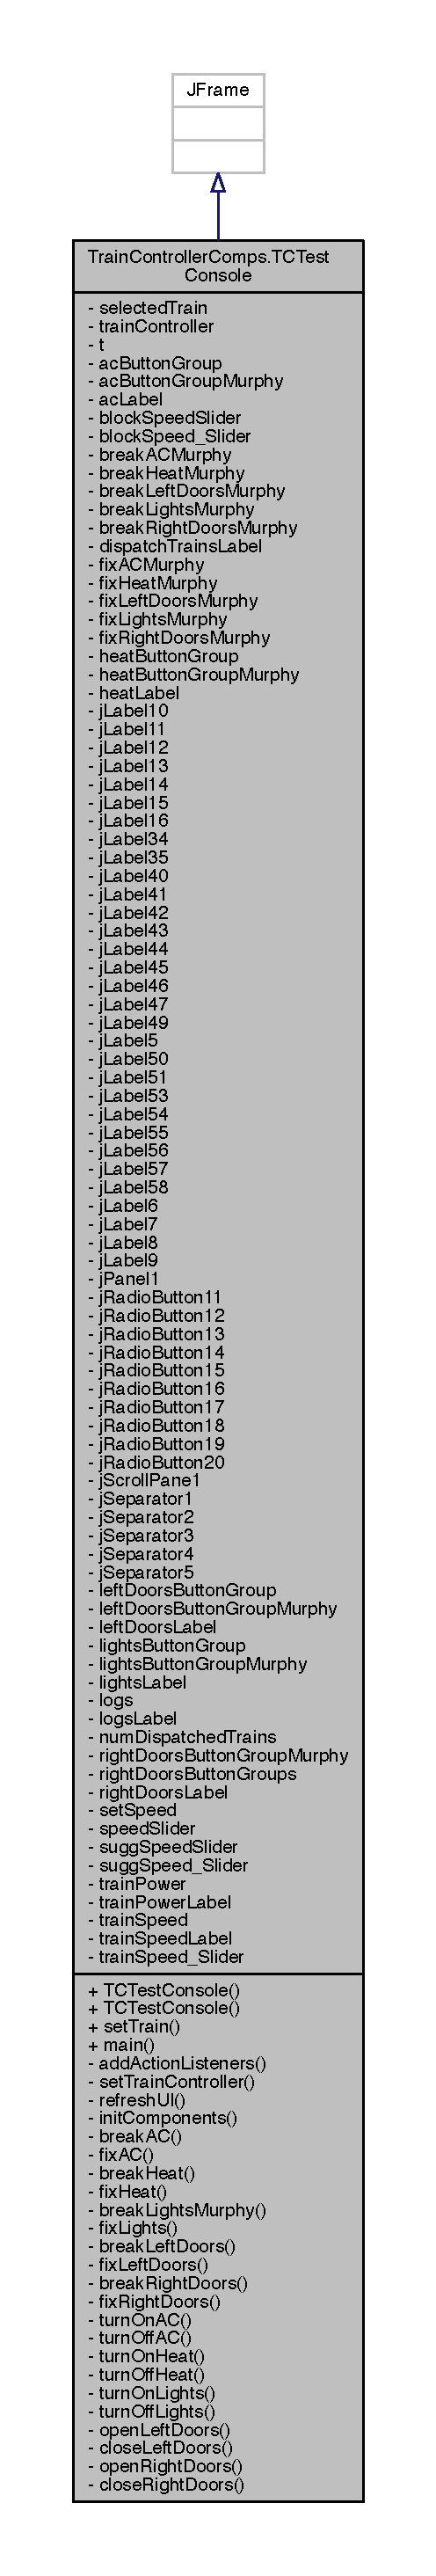
\includegraphics[height=550pt]{classTrainControllerComps_1_1TCTestConsole__inherit__graph}
\end{center}
\end{figure}


Collaboration diagram for Train\+Controller\+Comps.\+T\+C\+Test\+Console\+:
\nopagebreak
\begin{figure}[H]
\begin{center}
\leavevmode
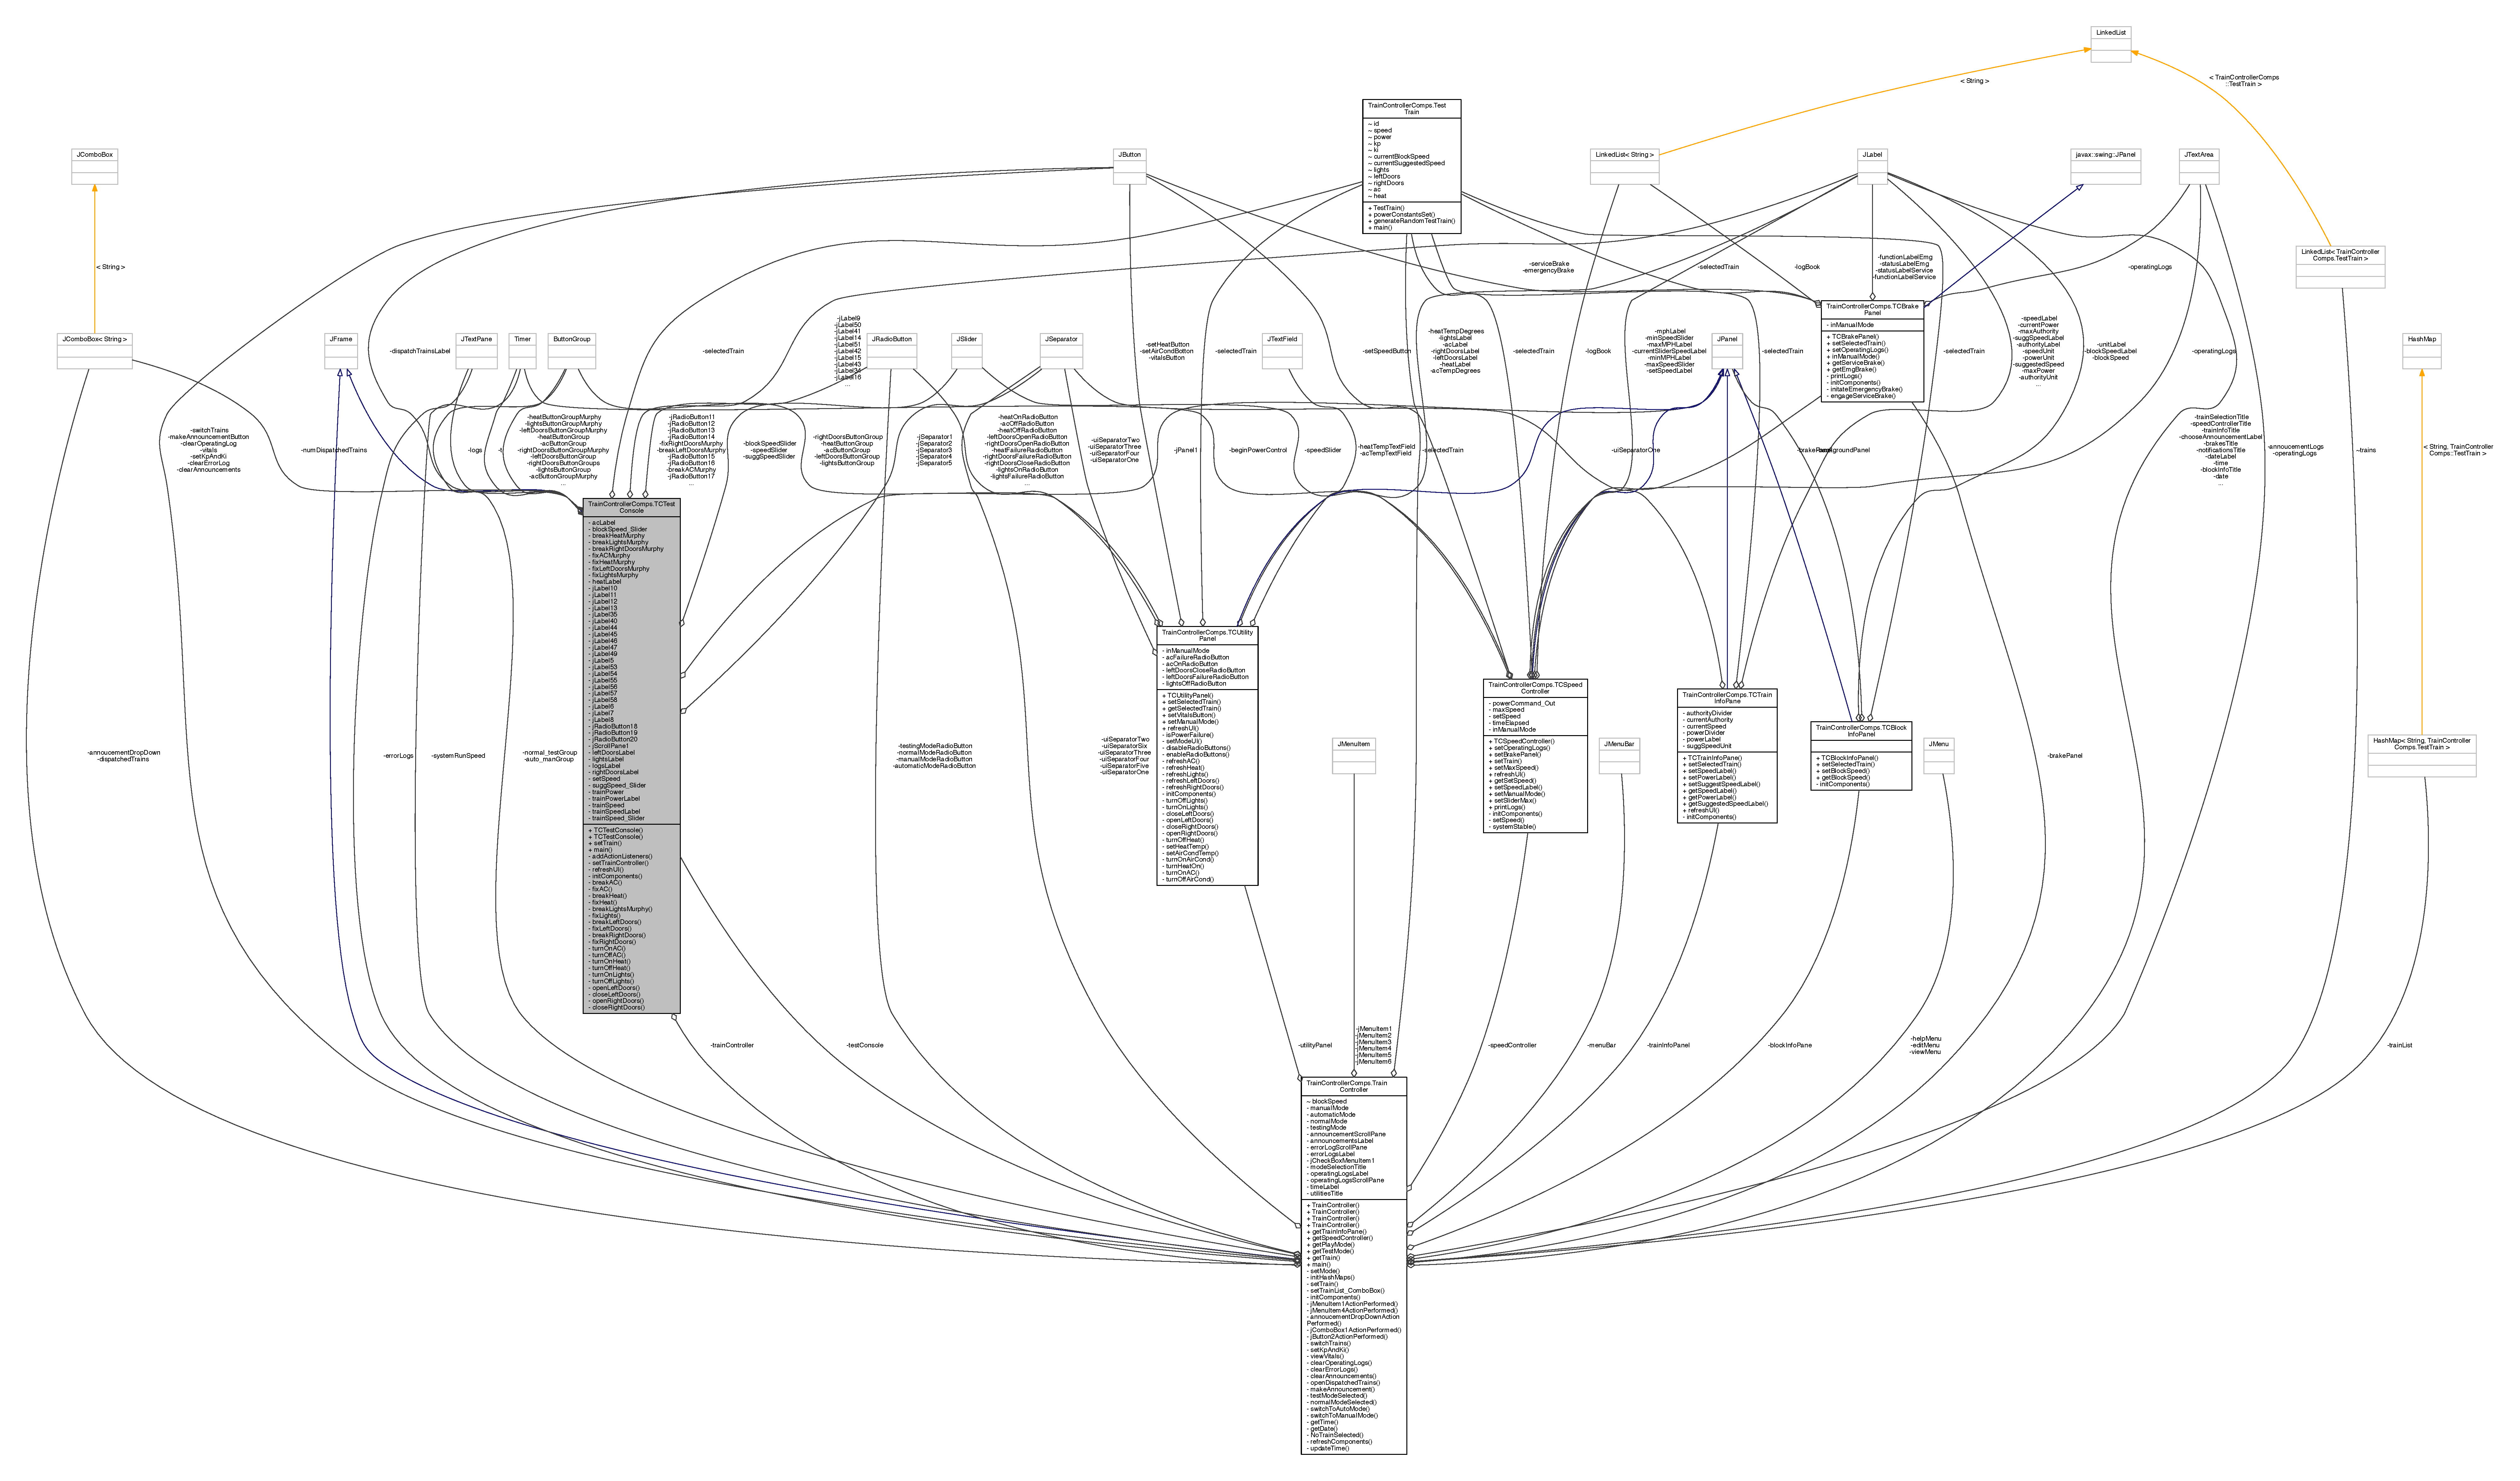
\includegraphics[width=350pt]{classTrainControllerComps_1_1TCTestConsole__coll__graph}
\end{center}
\end{figure}
\subsection*{Public Member Functions}
\begin{DoxyCompactItemize}
\item 
\hyperlink{classTrainControllerComps_1_1TCTestConsole_a760b79fd912301b36a19c372eafc1616}{T\+C\+Test\+Console} ()
\begin{DoxyCompactList}\small\item\em Constructor for creating a \hyperlink{classTrainControllerComps_1_1TCTestConsole}{T\+C\+Test\+Console} object with no Train Controller and no selected train. \end{DoxyCompactList}\item 
\hyperlink{classTrainControllerComps_1_1TCTestConsole_acb9494e195e57188bc7150aa96faef80}{T\+C\+Test\+Console} (\hyperlink{classTrainControllerComps_1_1TestTrain}{Test\+Train} \hyperlink{classtrain}{train}, \hyperlink{classTrainControllerComps_1_1TrainController}{Train\+Controller} train\+Cont)
\begin{DoxyCompactList}\small\item\em Creates new form \hyperlink{classTrainControllerComps_1_1TCTestConsole}{T\+C\+Test\+Console}. \end{DoxyCompactList}\item 
void \hyperlink{classTrainControllerComps_1_1TCTestConsole_a3519b295cbb041ec2af003311057f589}{set\+Train} (\hyperlink{classTrainControllerComps_1_1TestTrain}{Test\+Train} \hyperlink{classtrain}{train})
\end{DoxyCompactItemize}
\subsection*{Static Public Member Functions}
\begin{DoxyCompactItemize}
\item 
static void \hyperlink{classTrainControllerComps_1_1TCTestConsole_ac357695bde522e9b9f51b9b8231f6491}{main} (String args\mbox{[}$\,$\mbox{]})
\end{DoxyCompactItemize}
\subsection*{Private Member Functions}
\begin{DoxyCompactItemize}
\item 
void \hyperlink{classTrainControllerComps_1_1TCTestConsole_a6dbf679049bb88386a66eb60368f1e23}{add\+Action\+Listeners} ()
\begin{DoxyCompactList}\small\item\em Adds action listeners to their corresponding elements. \end{DoxyCompactList}\item 
void \hyperlink{classTrainControllerComps_1_1TCTestConsole_a44225d3560eda9d1d281a21b6c4d9793}{set\+Train\+Controller} (\hyperlink{classTrainControllerComps_1_1TrainController}{Train\+Controller} train\+Cont)
\item 
void \hyperlink{classTrainControllerComps_1_1TCTestConsole_a8c36f9ef39a0e5b17ff982eb9a5fb2d1}{refresh\+UI} ()
\item 
void \hyperlink{classTrainControllerComps_1_1TCTestConsole_a0ce4f7085d384256e806c978e19521cf}{init\+Components} ()
\begin{DoxyCompactList}\small\item\em This method is called from within the constructor to initialize the form. \end{DoxyCompactList}\item 
void \hyperlink{classTrainControllerComps_1_1TCTestConsole_a719ba5669ea8d3015b18f7534ac7aef8}{break\+AC} (java.\+awt.\+event.\+Action\+Event evt)
\item 
void \hyperlink{classTrainControllerComps_1_1TCTestConsole_aa21461aec8a7c5e82a16aa4170fd88d2}{fix\+AC} (java.\+awt.\+event.\+Action\+Event evt)
\item 
void \hyperlink{classTrainControllerComps_1_1TCTestConsole_a4183ab4b832ba4004efe36268e2d42e1}{break\+Heat} (java.\+awt.\+event.\+Action\+Event evt)
\item 
void \hyperlink{classTrainControllerComps_1_1TCTestConsole_a7567377a01ddf6773ee63a59f1f2fa24}{fix\+Heat} (java.\+awt.\+event.\+Action\+Event evt)
\item 
void \hyperlink{classTrainControllerComps_1_1TCTestConsole_ac653a53d3cf8290b2961434444b54295}{break\+Lights\+Murphy} (java.\+awt.\+event.\+Action\+Event evt)
\item 
void \hyperlink{classTrainControllerComps_1_1TCTestConsole_ad3e1912c4e49eaf33bf4ddaba7e1f090}{fix\+Lights} (java.\+awt.\+event.\+Action\+Event evt)
\item 
void \hyperlink{classTrainControllerComps_1_1TCTestConsole_a86123ba20ca1fbf0585820d0e314ea0e}{break\+Left\+Doors} (java.\+awt.\+event.\+Action\+Event evt)
\item 
void \hyperlink{classTrainControllerComps_1_1TCTestConsole_a074530680797980a0a59b89fd0825854}{fix\+Left\+Doors} (java.\+awt.\+event.\+Action\+Event evt)
\item 
void \hyperlink{classTrainControllerComps_1_1TCTestConsole_a58698a92444753ab9cf65df4eecbe23c}{break\+Right\+Doors} (java.\+awt.\+event.\+Action\+Event evt)
\item 
void \hyperlink{classTrainControllerComps_1_1TCTestConsole_aee30c912e6a071ea979f0629c5ad7f74}{fix\+Right\+Doors} (java.\+awt.\+event.\+Action\+Event evt)
\item 
void \hyperlink{classTrainControllerComps_1_1TCTestConsole_a2accf7ef6ebf4cc4014be09693138a57}{turn\+On\+AC} (java.\+awt.\+event.\+Action\+Event evt)
\item 
void \hyperlink{classTrainControllerComps_1_1TCTestConsole_a8350577198661578c091f8ae9f299ad4}{turn\+Off\+AC} (java.\+awt.\+event.\+Action\+Event evt)
\item 
void \hyperlink{classTrainControllerComps_1_1TCTestConsole_a7c9c0b19b82810b0b81f8405219e9ccb}{turn\+On\+Heat} (java.\+awt.\+event.\+Action\+Event evt)
\item 
void \hyperlink{classTrainControllerComps_1_1TCTestConsole_a37a58178270fbb1e271fd6d71a32313b}{turn\+Off\+Heat} (java.\+awt.\+event.\+Action\+Event evt)
\item 
void \hyperlink{classTrainControllerComps_1_1TCTestConsole_aa5f62334d031ea47f3275163b3042a96}{turn\+On\+Lights} (java.\+awt.\+event.\+Action\+Event evt)
\item 
void \hyperlink{classTrainControllerComps_1_1TCTestConsole_a1c52342312cab4d62b86bf4a52652703}{turn\+Off\+Lights} (java.\+awt.\+event.\+Action\+Event evt)
\item 
void \hyperlink{classTrainControllerComps_1_1TCTestConsole_a9e6b04de1514fc659dbf665a3dd1cf3d}{open\+Left\+Doors} (java.\+awt.\+event.\+Action\+Event evt)
\item 
void \hyperlink{classTrainControllerComps_1_1TCTestConsole_a0e23b1193885559198e02aa63c464e36}{close\+Left\+Doors} (java.\+awt.\+event.\+Action\+Event evt)
\item 
void \hyperlink{classTrainControllerComps_1_1TCTestConsole_ab960e72ee109ec472767cfd3dc7ef5fe}{open\+Right\+Doors} (java.\+awt.\+event.\+Action\+Event evt)
\item 
void \hyperlink{classTrainControllerComps_1_1TCTestConsole_af61e73d9719ecd0201ad535893ddca69}{close\+Right\+Doors} (java.\+awt.\+event.\+Action\+Event evt)
\end{DoxyCompactItemize}
\subsection*{Private Attributes}
\begin{DoxyCompactItemize}
\item 
\hyperlink{classTrainControllerComps_1_1TestTrain}{Test\+Train} \hyperlink{classTrainControllerComps_1_1TCTestConsole_a0d334010f5ee13f36d222a1e9c744692}{selected\+Train}
\begin{DoxyCompactList}\small\item\em Train being controlled by the Train Controller. \end{DoxyCompactList}\item 
\hyperlink{classTrainControllerComps_1_1TrainController}{Train\+Controller} \hyperlink{classTrainControllerComps_1_1TCTestConsole_a12271d14ee26a5ac90db1e541954b788}{train\+Controller}
\begin{DoxyCompactList}\small\item\em Train Controller to relay any changes made to the train to. \end{DoxyCompactList}\item 
Timer \hyperlink{classTrainControllerComps_1_1TCTestConsole_a30e4ba9897434ccc699b1d5cb1f80585}{t}
\begin{DoxyCompactList}\small\item\em Timer used to update the Test Console every 1 second. \end{DoxyCompactList}\item 
javax.\+swing.\+Button\+Group \hyperlink{classTrainControllerComps_1_1TCTestConsole_a8f84a548ccc7a10efb6a56bf1d9fb906}{ac\+Button\+Group}
\item 
javax.\+swing.\+Button\+Group \hyperlink{classTrainControllerComps_1_1TCTestConsole_a76ccb33a0cd9dae90633880b28844d19}{ac\+Button\+Group\+Murphy}
\item 
javax.\+swing.\+J\+Label \hyperlink{classTrainControllerComps_1_1TCTestConsole_af98035d73b1947ae389e67eeea4993c5}{ac\+Label}
\item 
javax.\+swing.\+J\+Slider \hyperlink{classTrainControllerComps_1_1TCTestConsole_a21bee125a17a7768a07a80d7783cf294}{block\+Speed\+Slider}
\item 
javax.\+swing.\+J\+Label \hyperlink{classTrainControllerComps_1_1TCTestConsole_ab79e1ccde06435df2e134bbe2a5f8742}{block\+Speed\+\_\+\+Slider}
\item 
javax.\+swing.\+J\+Radio\+Button \hyperlink{classTrainControllerComps_1_1TCTestConsole_a7d492665eb6c6971989ec2dc0466114a}{break\+A\+C\+Murphy}
\item 
javax.\+swing.\+J\+Radio\+Button \hyperlink{classTrainControllerComps_1_1TCTestConsole_a5a940e86e0d4401daea1572b40981510}{break\+Heat\+Murphy}
\item 
javax.\+swing.\+J\+Radio\+Button \hyperlink{classTrainControllerComps_1_1TCTestConsole_a684b806da57a86a664067abba549d03b}{break\+Left\+Doors\+Murphy}
\item 
javax.\+swing.\+J\+Radio\+Button \hyperlink{classTrainControllerComps_1_1TCTestConsole_accd7d43228d9317a1324e18187f3e037}{break\+Lights\+Murphy}
\item 
javax.\+swing.\+J\+Radio\+Button \hyperlink{classTrainControllerComps_1_1TCTestConsole_a66d910f995ad161cb6423f9609dc3410}{break\+Right\+Doors\+Murphy}
\item 
javax.\+swing.\+J\+Button \hyperlink{classTrainControllerComps_1_1TCTestConsole_ab1001e48d1473360905ff0456d2b6da2}{dispatch\+Trains\+Label}
\item 
javax.\+swing.\+J\+Radio\+Button \hyperlink{classTrainControllerComps_1_1TCTestConsole_a894040a202ec98ab18e585759f783d36}{fix\+A\+C\+Murphy}
\item 
javax.\+swing.\+J\+Radio\+Button \hyperlink{classTrainControllerComps_1_1TCTestConsole_aa536edd88e360f85dd5b3c183fb7bad7}{fix\+Heat\+Murphy}
\item 
javax.\+swing.\+J\+Radio\+Button \hyperlink{classTrainControllerComps_1_1TCTestConsole_af8181606847a064fef6388178f6345df}{fix\+Left\+Doors\+Murphy}
\item 
javax.\+swing.\+J\+Radio\+Button \hyperlink{classTrainControllerComps_1_1TCTestConsole_a64fb6ca41cae7641dc33c8095ffd9fdb}{fix\+Lights\+Murphy}
\item 
javax.\+swing.\+J\+Radio\+Button \hyperlink{classTrainControllerComps_1_1TCTestConsole_aa2c97390a7e262a469599bcb59f5a9c9}{fix\+Right\+Doors\+Murphy}
\item 
javax.\+swing.\+Button\+Group \hyperlink{classTrainControllerComps_1_1TCTestConsole_a652801186a60bbfa55e7a7da6e356eac}{heat\+Button\+Group}
\item 
javax.\+swing.\+Button\+Group \hyperlink{classTrainControllerComps_1_1TCTestConsole_a1e24f88e3c130a9197c58398af71062b}{heat\+Button\+Group\+Murphy}
\item 
javax.\+swing.\+J\+Label \hyperlink{classTrainControllerComps_1_1TCTestConsole_ad009dbddef64d4cf00a17e75888599b1}{heat\+Label}
\item 
javax.\+swing.\+J\+Label \hyperlink{classTrainControllerComps_1_1TCTestConsole_afe6f59cd0dbb68f59d14d44937a20560}{j\+Label10}
\item 
javax.\+swing.\+J\+Label \hyperlink{classTrainControllerComps_1_1TCTestConsole_aedd451e4b3cb09d6204b76ad2300b40c}{j\+Label11}
\item 
javax.\+swing.\+J\+Label \hyperlink{classTrainControllerComps_1_1TCTestConsole_a007650252cf57b42e6de59a615d09728}{j\+Label12}
\item 
javax.\+swing.\+J\+Label \hyperlink{classTrainControllerComps_1_1TCTestConsole_a33d57c87dbe079fd23e3c74b00267c32}{j\+Label13}
\item 
javax.\+swing.\+J\+Label \hyperlink{classTrainControllerComps_1_1TCTestConsole_af255f1641c06bd410b59a7053693bae3}{j\+Label14}
\item 
javax.\+swing.\+J\+Label \hyperlink{classTrainControllerComps_1_1TCTestConsole_a15c9eee45ab19ef43c58bc649724616c}{j\+Label15}
\item 
javax.\+swing.\+J\+Label \hyperlink{classTrainControllerComps_1_1TCTestConsole_af9018c9d636ebc614bf81ede1c548656}{j\+Label16}
\item 
javax.\+swing.\+J\+Label \hyperlink{classTrainControllerComps_1_1TCTestConsole_a569a1a8efd99421bfbceab4312397ea1}{j\+Label34}
\item 
javax.\+swing.\+J\+Label \hyperlink{classTrainControllerComps_1_1TCTestConsole_a44eb572be1c20e76bce8193253e7c88f}{j\+Label35}
\item 
javax.\+swing.\+J\+Label \hyperlink{classTrainControllerComps_1_1TCTestConsole_a47b53ca5ad512b2b9ad8d1595bd9e0f5}{j\+Label40}
\item 
javax.\+swing.\+J\+Label \hyperlink{classTrainControllerComps_1_1TCTestConsole_ad200ed7938f299f879fa78afe898737f}{j\+Label41}
\item 
javax.\+swing.\+J\+Label \hyperlink{classTrainControllerComps_1_1TCTestConsole_a0c9860acba538f840d14c3c8196539a4}{j\+Label42}
\item 
javax.\+swing.\+J\+Label \hyperlink{classTrainControllerComps_1_1TCTestConsole_a30909cde3d4367014b41b9cdbb745e97}{j\+Label43}
\item 
javax.\+swing.\+J\+Label \hyperlink{classTrainControllerComps_1_1TCTestConsole_a74d463fb2ef1d28d74b44c0102f86b12}{j\+Label44}
\item 
javax.\+swing.\+J\+Label \hyperlink{classTrainControllerComps_1_1TCTestConsole_ab9c1736625460c06ef2d293c09c6207d}{j\+Label45}
\item 
javax.\+swing.\+J\+Label \hyperlink{classTrainControllerComps_1_1TCTestConsole_ad9411cc13252f071cbed7d084bc8c6e7}{j\+Label46}
\item 
javax.\+swing.\+J\+Label \hyperlink{classTrainControllerComps_1_1TCTestConsole_a61e5a756963f60a5cab19f7772d3c81f}{j\+Label47}
\item 
javax.\+swing.\+J\+Label \hyperlink{classTrainControllerComps_1_1TCTestConsole_a3749f75bf110d43030c9085761c0457b}{j\+Label49}
\item 
javax.\+swing.\+J\+Label \hyperlink{classTrainControllerComps_1_1TCTestConsole_affacc4bea050e28768832ed436c66da7}{j\+Label5}
\item 
javax.\+swing.\+J\+Label \hyperlink{classTrainControllerComps_1_1TCTestConsole_acea7edb9ff737a8e16ce6ec754809d62}{j\+Label50}
\item 
javax.\+swing.\+J\+Label \hyperlink{classTrainControllerComps_1_1TCTestConsole_a95cb47604da863b779ad035d35025b30}{j\+Label51}
\item 
javax.\+swing.\+J\+Label \hyperlink{classTrainControllerComps_1_1TCTestConsole_ad67cc6b4ae4473c6eb60bc8fd3bdfa75}{j\+Label53}
\item 
javax.\+swing.\+J\+Label \hyperlink{classTrainControllerComps_1_1TCTestConsole_af0ca5db132c0010e64199a33f6891241}{j\+Label54}
\item 
javax.\+swing.\+J\+Label \hyperlink{classTrainControllerComps_1_1TCTestConsole_ac5fa3f2159a209efa8e735c5d04034f4}{j\+Label55}
\item 
javax.\+swing.\+J\+Label \hyperlink{classTrainControllerComps_1_1TCTestConsole_a29c4733bf5f643ca90431e82e8ef3bc0}{j\+Label56}
\item 
javax.\+swing.\+J\+Label \hyperlink{classTrainControllerComps_1_1TCTestConsole_a3f0313a94952835cb25fbf21dae9ef04}{j\+Label57}
\item 
javax.\+swing.\+J\+Label \hyperlink{classTrainControllerComps_1_1TCTestConsole_a4423420eca93e1713f59742dc8ac48fc}{j\+Label58}
\item 
javax.\+swing.\+J\+Label \hyperlink{classTrainControllerComps_1_1TCTestConsole_a295d6d79a5053490f1e9ed4f49063369}{j\+Label6}
\item 
javax.\+swing.\+J\+Label \hyperlink{classTrainControllerComps_1_1TCTestConsole_a56061314e64982fd14f12f8c157bc446}{j\+Label7}
\item 
javax.\+swing.\+J\+Label \hyperlink{classTrainControllerComps_1_1TCTestConsole_af5c88ee6fdf8514186e4be2e0367222d}{j\+Label8}
\item 
javax.\+swing.\+J\+Label \hyperlink{classTrainControllerComps_1_1TCTestConsole_a82965e977b9eab5384711fa7dae2c7df}{j\+Label9}
\item 
javax.\+swing.\+J\+Panel \hyperlink{classTrainControllerComps_1_1TCTestConsole_af78b45798e2b3493704987ebd4fcdec5}{j\+Panel1}
\item 
javax.\+swing.\+J\+Radio\+Button \hyperlink{classTrainControllerComps_1_1TCTestConsole_a4841a010a5d290e5ccd4ab08c0660cdd}{j\+Radio\+Button11}
\item 
javax.\+swing.\+J\+Radio\+Button \hyperlink{classTrainControllerComps_1_1TCTestConsole_afabaa89b5791c44f113a704f26f0653d}{j\+Radio\+Button12}
\item 
javax.\+swing.\+J\+Radio\+Button \hyperlink{classTrainControllerComps_1_1TCTestConsole_aba8a4cf1aec37a400b88f24df6e6b00f}{j\+Radio\+Button13}
\item 
javax.\+swing.\+J\+Radio\+Button \hyperlink{classTrainControllerComps_1_1TCTestConsole_ac8e7e27aa2da7d8b20473de214f55545}{j\+Radio\+Button14}
\item 
javax.\+swing.\+J\+Radio\+Button \hyperlink{classTrainControllerComps_1_1TCTestConsole_a0ae60a752f0dba23f979a55cb862751f}{j\+Radio\+Button15}
\item 
javax.\+swing.\+J\+Radio\+Button \hyperlink{classTrainControllerComps_1_1TCTestConsole_aec997692de4894a4428e3bf6b665d319}{j\+Radio\+Button16}
\item 
javax.\+swing.\+J\+Radio\+Button \hyperlink{classTrainControllerComps_1_1TCTestConsole_aa0785089513677993651b2ec2401acd9}{j\+Radio\+Button17}
\item 
javax.\+swing.\+J\+Radio\+Button \hyperlink{classTrainControllerComps_1_1TCTestConsole_af96dfe5ab6c3939fd1f1107052b32860}{j\+Radio\+Button18}
\item 
javax.\+swing.\+J\+Radio\+Button \hyperlink{classTrainControllerComps_1_1TCTestConsole_add689f3cb879f656ce537f7b0de37790}{j\+Radio\+Button19}
\item 
javax.\+swing.\+J\+Radio\+Button \hyperlink{classTrainControllerComps_1_1TCTestConsole_a637db2168f9d0e3c3d36b084fe376667}{j\+Radio\+Button20}
\item 
javax.\+swing.\+J\+Scroll\+Pane \hyperlink{classTrainControllerComps_1_1TCTestConsole_a5ee544c3a96aebcfc3fb359811f53e17}{j\+Scroll\+Pane1}
\item 
javax.\+swing.\+J\+Separator \hyperlink{classTrainControllerComps_1_1TCTestConsole_aa6e341ad4a933305c208ddfab87b7748}{j\+Separator1}
\item 
javax.\+swing.\+J\+Separator \hyperlink{classTrainControllerComps_1_1TCTestConsole_a321b1c444b86da9a4c8dd6a5e5206d44}{j\+Separator2}
\item 
javax.\+swing.\+J\+Separator \hyperlink{classTrainControllerComps_1_1TCTestConsole_aeb40f199fd2cfcb8f20110d13ddc43ae}{j\+Separator3}
\item 
javax.\+swing.\+J\+Separator \hyperlink{classTrainControllerComps_1_1TCTestConsole_ab4b1231ce9b294b2765bb91c44522e3c}{j\+Separator4}
\item 
javax.\+swing.\+J\+Separator \hyperlink{classTrainControllerComps_1_1TCTestConsole_a5907933373af800e343932b74f2b5953}{j\+Separator5}
\item 
javax.\+swing.\+Button\+Group \hyperlink{classTrainControllerComps_1_1TCTestConsole_a6e9e34dbae54de3d18973079a119b259}{left\+Doors\+Button\+Group}
\item 
javax.\+swing.\+Button\+Group \hyperlink{classTrainControllerComps_1_1TCTestConsole_a31e351b69749abd5011ab27db71f2c93}{left\+Doors\+Button\+Group\+Murphy}
\item 
javax.\+swing.\+J\+Label \hyperlink{classTrainControllerComps_1_1TCTestConsole_a019c8a0ab8654c401c1e34d4d02237f9}{left\+Doors\+Label}
\item 
javax.\+swing.\+Button\+Group \hyperlink{classTrainControllerComps_1_1TCTestConsole_a19ea08b80e017c2370d6a71e6f2c9688}{lights\+Button\+Group}
\item 
javax.\+swing.\+Button\+Group \hyperlink{classTrainControllerComps_1_1TCTestConsole_ade57cb3a0c1580b921e0ff5ad758c80a}{lights\+Button\+Group\+Murphy}
\item 
javax.\+swing.\+J\+Label \hyperlink{classTrainControllerComps_1_1TCTestConsole_ac6b7301f535cea9ef8d39ba8d9e21bc3}{lights\+Label}
\item 
javax.\+swing.\+J\+Text\+Pane \hyperlink{classTrainControllerComps_1_1TCTestConsole_acb8f9a2f8b463f489504ceb2632e0472}{logs}
\item 
javax.\+swing.\+J\+Label \hyperlink{classTrainControllerComps_1_1TCTestConsole_a863cecfa16a93d7a4e220853a7202a80}{logs\+Label}
\item 
javax.\+swing.\+J\+Combo\+Box$<$ String $>$ \hyperlink{classTrainControllerComps_1_1TCTestConsole_af08c073d08ed471e509709158a0ca2d3}{num\+Dispatched\+Trains}
\item 
javax.\+swing.\+Button\+Group \hyperlink{classTrainControllerComps_1_1TCTestConsole_a857ac857bbf765132239734e62c78210}{right\+Doors\+Button\+Group\+Murphy}
\item 
javax.\+swing.\+Button\+Group \hyperlink{classTrainControllerComps_1_1TCTestConsole_a5fd502aa4588d4ec5d4503cad1dc399c}{right\+Doors\+Button\+Groups}
\item 
javax.\+swing.\+J\+Label \hyperlink{classTrainControllerComps_1_1TCTestConsole_a9305662f0767e36bf1f990834b73cfc3}{right\+Doors\+Label}
\item 
javax.\+swing.\+J\+Label \hyperlink{classTrainControllerComps_1_1TCTestConsole_ad8105908c48ad8b5fd4c0a951db655a2}{set\+Speed}
\item 
javax.\+swing.\+J\+Slider \hyperlink{classTrainControllerComps_1_1TCTestConsole_a493fcafc1264f633059e840f83207593}{speed\+Slider}
\item 
javax.\+swing.\+J\+Slider \hyperlink{classTrainControllerComps_1_1TCTestConsole_a9d7e5b560ae353604fe3281c949dc2a7}{sugg\+Speed\+Slider}
\item 
javax.\+swing.\+J\+Label \hyperlink{classTrainControllerComps_1_1TCTestConsole_af9f54adad63841cba14c0bbb41ab3de7}{sugg\+Speed\+\_\+\+Slider}
\item 
javax.\+swing.\+J\+Label \hyperlink{classTrainControllerComps_1_1TCTestConsole_a1e94ccf980f441f8e7c411ed38c42be5}{train\+Power}
\item 
javax.\+swing.\+J\+Label \hyperlink{classTrainControllerComps_1_1TCTestConsole_ac2dc24779140f31fd6f33be4be926c96}{train\+Power\+Label}
\item 
javax.\+swing.\+J\+Label \hyperlink{classTrainControllerComps_1_1TCTestConsole_a5ffb3ab5c0f9a7fc37f72c77e70432a9}{train\+Speed}
\item 
javax.\+swing.\+J\+Label \hyperlink{classTrainControllerComps_1_1TCTestConsole_a6d89bc3a12936a14165ba016d51df6b6}{train\+Speed\+Label}
\item 
javax.\+swing.\+J\+Label \hyperlink{classTrainControllerComps_1_1TCTestConsole_a4fbf210d4a143467d39d3311171422dd}{train\+Speed\+\_\+\+Slider}
\end{DoxyCompactItemize}


\subsection{Detailed Description}
This class is responsible for testing the various components in the Train Controller, mimicking the components on a train object. 

This class collaborates with the Train Controller and Train class.

\begin{DoxyAuthor}{Author}
Andrew Lendacky 
\end{DoxyAuthor}


\subsection{Constructor \& Destructor Documentation}
\mbox{\Hypertarget{classTrainControllerComps_1_1TCTestConsole_a760b79fd912301b36a19c372eafc1616}\label{classTrainControllerComps_1_1TCTestConsole_a760b79fd912301b36a19c372eafc1616}} 
\index{Train\+Controller\+Comps\+::\+T\+C\+Test\+Console@{Train\+Controller\+Comps\+::\+T\+C\+Test\+Console}!T\+C\+Test\+Console@{T\+C\+Test\+Console}}
\index{T\+C\+Test\+Console@{T\+C\+Test\+Console}!Train\+Controller\+Comps\+::\+T\+C\+Test\+Console@{Train\+Controller\+Comps\+::\+T\+C\+Test\+Console}}
\subsubsection{\texorpdfstring{T\+C\+Test\+Console()}{TCTestConsole()}\hspace{0.1cm}{\footnotesize\ttfamily [1/2]}}
{\footnotesize\ttfamily Train\+Controller\+Comps.\+T\+C\+Test\+Console.\+T\+C\+Test\+Console (\begin{DoxyParamCaption}{ }\end{DoxyParamCaption})}



Constructor for creating a \hyperlink{classTrainControllerComps_1_1TCTestConsole}{T\+C\+Test\+Console} object with no Train Controller and no selected train. 

\mbox{\Hypertarget{classTrainControllerComps_1_1TCTestConsole_acb9494e195e57188bc7150aa96faef80}\label{classTrainControllerComps_1_1TCTestConsole_acb9494e195e57188bc7150aa96faef80}} 
\index{Train\+Controller\+Comps\+::\+T\+C\+Test\+Console@{Train\+Controller\+Comps\+::\+T\+C\+Test\+Console}!T\+C\+Test\+Console@{T\+C\+Test\+Console}}
\index{T\+C\+Test\+Console@{T\+C\+Test\+Console}!Train\+Controller\+Comps\+::\+T\+C\+Test\+Console@{Train\+Controller\+Comps\+::\+T\+C\+Test\+Console}}
\subsubsection{\texorpdfstring{T\+C\+Test\+Console()}{TCTestConsole()}\hspace{0.1cm}{\footnotesize\ttfamily [2/2]}}
{\footnotesize\ttfamily Train\+Controller\+Comps.\+T\+C\+Test\+Console.\+T\+C\+Test\+Console (\begin{DoxyParamCaption}\item[{\hyperlink{classTrainControllerComps_1_1TestTrain}{Test\+Train}}]{train,  }\item[{\hyperlink{classTrainControllerComps_1_1TrainController}{Train\+Controller}}]{train\+Cont }\end{DoxyParamCaption})}



Creates new form \hyperlink{classTrainControllerComps_1_1TCTestConsole}{T\+C\+Test\+Console}. 



\subsection{Member Function Documentation}
\mbox{\Hypertarget{classTrainControllerComps_1_1TCTestConsole_a6dbf679049bb88386a66eb60368f1e23}\label{classTrainControllerComps_1_1TCTestConsole_a6dbf679049bb88386a66eb60368f1e23}} 
\index{Train\+Controller\+Comps\+::\+T\+C\+Test\+Console@{Train\+Controller\+Comps\+::\+T\+C\+Test\+Console}!add\+Action\+Listeners@{add\+Action\+Listeners}}
\index{add\+Action\+Listeners@{add\+Action\+Listeners}!Train\+Controller\+Comps\+::\+T\+C\+Test\+Console@{Train\+Controller\+Comps\+::\+T\+C\+Test\+Console}}
\subsubsection{\texorpdfstring{add\+Action\+Listeners()}{addActionListeners()}}
{\footnotesize\ttfamily void Train\+Controller\+Comps.\+T\+C\+Test\+Console.\+add\+Action\+Listeners (\begin{DoxyParamCaption}{ }\end{DoxyParamCaption})\hspace{0.3cm}{\ttfamily [private]}}



Adds action listeners to their corresponding elements. 

\mbox{\Hypertarget{classTrainControllerComps_1_1TCTestConsole_a719ba5669ea8d3015b18f7534ac7aef8}\label{classTrainControllerComps_1_1TCTestConsole_a719ba5669ea8d3015b18f7534ac7aef8}} 
\index{Train\+Controller\+Comps\+::\+T\+C\+Test\+Console@{Train\+Controller\+Comps\+::\+T\+C\+Test\+Console}!break\+AC@{break\+AC}}
\index{break\+AC@{break\+AC}!Train\+Controller\+Comps\+::\+T\+C\+Test\+Console@{Train\+Controller\+Comps\+::\+T\+C\+Test\+Console}}
\subsubsection{\texorpdfstring{break\+A\+C()}{breakAC()}}
{\footnotesize\ttfamily void Train\+Controller\+Comps.\+T\+C\+Test\+Console.\+break\+AC (\begin{DoxyParamCaption}\item[{java.\+awt.\+event.\+Action\+Event}]{evt }\end{DoxyParamCaption})\hspace{0.3cm}{\ttfamily [private]}}

\mbox{\Hypertarget{classTrainControllerComps_1_1TCTestConsole_a4183ab4b832ba4004efe36268e2d42e1}\label{classTrainControllerComps_1_1TCTestConsole_a4183ab4b832ba4004efe36268e2d42e1}} 
\index{Train\+Controller\+Comps\+::\+T\+C\+Test\+Console@{Train\+Controller\+Comps\+::\+T\+C\+Test\+Console}!break\+Heat@{break\+Heat}}
\index{break\+Heat@{break\+Heat}!Train\+Controller\+Comps\+::\+T\+C\+Test\+Console@{Train\+Controller\+Comps\+::\+T\+C\+Test\+Console}}
\subsubsection{\texorpdfstring{break\+Heat()}{breakHeat()}}
{\footnotesize\ttfamily void Train\+Controller\+Comps.\+T\+C\+Test\+Console.\+break\+Heat (\begin{DoxyParamCaption}\item[{java.\+awt.\+event.\+Action\+Event}]{evt }\end{DoxyParamCaption})\hspace{0.3cm}{\ttfamily [private]}}

\mbox{\Hypertarget{classTrainControllerComps_1_1TCTestConsole_a86123ba20ca1fbf0585820d0e314ea0e}\label{classTrainControllerComps_1_1TCTestConsole_a86123ba20ca1fbf0585820d0e314ea0e}} 
\index{Train\+Controller\+Comps\+::\+T\+C\+Test\+Console@{Train\+Controller\+Comps\+::\+T\+C\+Test\+Console}!break\+Left\+Doors@{break\+Left\+Doors}}
\index{break\+Left\+Doors@{break\+Left\+Doors}!Train\+Controller\+Comps\+::\+T\+C\+Test\+Console@{Train\+Controller\+Comps\+::\+T\+C\+Test\+Console}}
\subsubsection{\texorpdfstring{break\+Left\+Doors()}{breakLeftDoors()}}
{\footnotesize\ttfamily void Train\+Controller\+Comps.\+T\+C\+Test\+Console.\+break\+Left\+Doors (\begin{DoxyParamCaption}\item[{java.\+awt.\+event.\+Action\+Event}]{evt }\end{DoxyParamCaption})\hspace{0.3cm}{\ttfamily [private]}}

\mbox{\Hypertarget{classTrainControllerComps_1_1TCTestConsole_ac653a53d3cf8290b2961434444b54295}\label{classTrainControllerComps_1_1TCTestConsole_ac653a53d3cf8290b2961434444b54295}} 
\index{Train\+Controller\+Comps\+::\+T\+C\+Test\+Console@{Train\+Controller\+Comps\+::\+T\+C\+Test\+Console}!break\+Lights\+Murphy@{break\+Lights\+Murphy}}
\index{break\+Lights\+Murphy@{break\+Lights\+Murphy}!Train\+Controller\+Comps\+::\+T\+C\+Test\+Console@{Train\+Controller\+Comps\+::\+T\+C\+Test\+Console}}
\subsubsection{\texorpdfstring{break\+Lights\+Murphy()}{breakLightsMurphy()}}
{\footnotesize\ttfamily void Train\+Controller\+Comps.\+T\+C\+Test\+Console.\+break\+Lights\+Murphy (\begin{DoxyParamCaption}\item[{java.\+awt.\+event.\+Action\+Event}]{evt }\end{DoxyParamCaption})\hspace{0.3cm}{\ttfamily [private]}}

\mbox{\Hypertarget{classTrainControllerComps_1_1TCTestConsole_a58698a92444753ab9cf65df4eecbe23c}\label{classTrainControllerComps_1_1TCTestConsole_a58698a92444753ab9cf65df4eecbe23c}} 
\index{Train\+Controller\+Comps\+::\+T\+C\+Test\+Console@{Train\+Controller\+Comps\+::\+T\+C\+Test\+Console}!break\+Right\+Doors@{break\+Right\+Doors}}
\index{break\+Right\+Doors@{break\+Right\+Doors}!Train\+Controller\+Comps\+::\+T\+C\+Test\+Console@{Train\+Controller\+Comps\+::\+T\+C\+Test\+Console}}
\subsubsection{\texorpdfstring{break\+Right\+Doors()}{breakRightDoors()}}
{\footnotesize\ttfamily void Train\+Controller\+Comps.\+T\+C\+Test\+Console.\+break\+Right\+Doors (\begin{DoxyParamCaption}\item[{java.\+awt.\+event.\+Action\+Event}]{evt }\end{DoxyParamCaption})\hspace{0.3cm}{\ttfamily [private]}}

\mbox{\Hypertarget{classTrainControllerComps_1_1TCTestConsole_a0e23b1193885559198e02aa63c464e36}\label{classTrainControllerComps_1_1TCTestConsole_a0e23b1193885559198e02aa63c464e36}} 
\index{Train\+Controller\+Comps\+::\+T\+C\+Test\+Console@{Train\+Controller\+Comps\+::\+T\+C\+Test\+Console}!close\+Left\+Doors@{close\+Left\+Doors}}
\index{close\+Left\+Doors@{close\+Left\+Doors}!Train\+Controller\+Comps\+::\+T\+C\+Test\+Console@{Train\+Controller\+Comps\+::\+T\+C\+Test\+Console}}
\subsubsection{\texorpdfstring{close\+Left\+Doors()}{closeLeftDoors()}}
{\footnotesize\ttfamily void Train\+Controller\+Comps.\+T\+C\+Test\+Console.\+close\+Left\+Doors (\begin{DoxyParamCaption}\item[{java.\+awt.\+event.\+Action\+Event}]{evt }\end{DoxyParamCaption})\hspace{0.3cm}{\ttfamily [private]}}

\mbox{\Hypertarget{classTrainControllerComps_1_1TCTestConsole_af61e73d9719ecd0201ad535893ddca69}\label{classTrainControllerComps_1_1TCTestConsole_af61e73d9719ecd0201ad535893ddca69}} 
\index{Train\+Controller\+Comps\+::\+T\+C\+Test\+Console@{Train\+Controller\+Comps\+::\+T\+C\+Test\+Console}!close\+Right\+Doors@{close\+Right\+Doors}}
\index{close\+Right\+Doors@{close\+Right\+Doors}!Train\+Controller\+Comps\+::\+T\+C\+Test\+Console@{Train\+Controller\+Comps\+::\+T\+C\+Test\+Console}}
\subsubsection{\texorpdfstring{close\+Right\+Doors()}{closeRightDoors()}}
{\footnotesize\ttfamily void Train\+Controller\+Comps.\+T\+C\+Test\+Console.\+close\+Right\+Doors (\begin{DoxyParamCaption}\item[{java.\+awt.\+event.\+Action\+Event}]{evt }\end{DoxyParamCaption})\hspace{0.3cm}{\ttfamily [private]}}

\mbox{\Hypertarget{classTrainControllerComps_1_1TCTestConsole_aa21461aec8a7c5e82a16aa4170fd88d2}\label{classTrainControllerComps_1_1TCTestConsole_aa21461aec8a7c5e82a16aa4170fd88d2}} 
\index{Train\+Controller\+Comps\+::\+T\+C\+Test\+Console@{Train\+Controller\+Comps\+::\+T\+C\+Test\+Console}!fix\+AC@{fix\+AC}}
\index{fix\+AC@{fix\+AC}!Train\+Controller\+Comps\+::\+T\+C\+Test\+Console@{Train\+Controller\+Comps\+::\+T\+C\+Test\+Console}}
\subsubsection{\texorpdfstring{fix\+A\+C()}{fixAC()}}
{\footnotesize\ttfamily void Train\+Controller\+Comps.\+T\+C\+Test\+Console.\+fix\+AC (\begin{DoxyParamCaption}\item[{java.\+awt.\+event.\+Action\+Event}]{evt }\end{DoxyParamCaption})\hspace{0.3cm}{\ttfamily [private]}}

\mbox{\Hypertarget{classTrainControllerComps_1_1TCTestConsole_a7567377a01ddf6773ee63a59f1f2fa24}\label{classTrainControllerComps_1_1TCTestConsole_a7567377a01ddf6773ee63a59f1f2fa24}} 
\index{Train\+Controller\+Comps\+::\+T\+C\+Test\+Console@{Train\+Controller\+Comps\+::\+T\+C\+Test\+Console}!fix\+Heat@{fix\+Heat}}
\index{fix\+Heat@{fix\+Heat}!Train\+Controller\+Comps\+::\+T\+C\+Test\+Console@{Train\+Controller\+Comps\+::\+T\+C\+Test\+Console}}
\subsubsection{\texorpdfstring{fix\+Heat()}{fixHeat()}}
{\footnotesize\ttfamily void Train\+Controller\+Comps.\+T\+C\+Test\+Console.\+fix\+Heat (\begin{DoxyParamCaption}\item[{java.\+awt.\+event.\+Action\+Event}]{evt }\end{DoxyParamCaption})\hspace{0.3cm}{\ttfamily [private]}}

\mbox{\Hypertarget{classTrainControllerComps_1_1TCTestConsole_a074530680797980a0a59b89fd0825854}\label{classTrainControllerComps_1_1TCTestConsole_a074530680797980a0a59b89fd0825854}} 
\index{Train\+Controller\+Comps\+::\+T\+C\+Test\+Console@{Train\+Controller\+Comps\+::\+T\+C\+Test\+Console}!fix\+Left\+Doors@{fix\+Left\+Doors}}
\index{fix\+Left\+Doors@{fix\+Left\+Doors}!Train\+Controller\+Comps\+::\+T\+C\+Test\+Console@{Train\+Controller\+Comps\+::\+T\+C\+Test\+Console}}
\subsubsection{\texorpdfstring{fix\+Left\+Doors()}{fixLeftDoors()}}
{\footnotesize\ttfamily void Train\+Controller\+Comps.\+T\+C\+Test\+Console.\+fix\+Left\+Doors (\begin{DoxyParamCaption}\item[{java.\+awt.\+event.\+Action\+Event}]{evt }\end{DoxyParamCaption})\hspace{0.3cm}{\ttfamily [private]}}

\mbox{\Hypertarget{classTrainControllerComps_1_1TCTestConsole_ad3e1912c4e49eaf33bf4ddaba7e1f090}\label{classTrainControllerComps_1_1TCTestConsole_ad3e1912c4e49eaf33bf4ddaba7e1f090}} 
\index{Train\+Controller\+Comps\+::\+T\+C\+Test\+Console@{Train\+Controller\+Comps\+::\+T\+C\+Test\+Console}!fix\+Lights@{fix\+Lights}}
\index{fix\+Lights@{fix\+Lights}!Train\+Controller\+Comps\+::\+T\+C\+Test\+Console@{Train\+Controller\+Comps\+::\+T\+C\+Test\+Console}}
\subsubsection{\texorpdfstring{fix\+Lights()}{fixLights()}}
{\footnotesize\ttfamily void Train\+Controller\+Comps.\+T\+C\+Test\+Console.\+fix\+Lights (\begin{DoxyParamCaption}\item[{java.\+awt.\+event.\+Action\+Event}]{evt }\end{DoxyParamCaption})\hspace{0.3cm}{\ttfamily [private]}}

\mbox{\Hypertarget{classTrainControllerComps_1_1TCTestConsole_aee30c912e6a071ea979f0629c5ad7f74}\label{classTrainControllerComps_1_1TCTestConsole_aee30c912e6a071ea979f0629c5ad7f74}} 
\index{Train\+Controller\+Comps\+::\+T\+C\+Test\+Console@{Train\+Controller\+Comps\+::\+T\+C\+Test\+Console}!fix\+Right\+Doors@{fix\+Right\+Doors}}
\index{fix\+Right\+Doors@{fix\+Right\+Doors}!Train\+Controller\+Comps\+::\+T\+C\+Test\+Console@{Train\+Controller\+Comps\+::\+T\+C\+Test\+Console}}
\subsubsection{\texorpdfstring{fix\+Right\+Doors()}{fixRightDoors()}}
{\footnotesize\ttfamily void Train\+Controller\+Comps.\+T\+C\+Test\+Console.\+fix\+Right\+Doors (\begin{DoxyParamCaption}\item[{java.\+awt.\+event.\+Action\+Event}]{evt }\end{DoxyParamCaption})\hspace{0.3cm}{\ttfamily [private]}}

\mbox{\Hypertarget{classTrainControllerComps_1_1TCTestConsole_a0ce4f7085d384256e806c978e19521cf}\label{classTrainControllerComps_1_1TCTestConsole_a0ce4f7085d384256e806c978e19521cf}} 
\index{Train\+Controller\+Comps\+::\+T\+C\+Test\+Console@{Train\+Controller\+Comps\+::\+T\+C\+Test\+Console}!init\+Components@{init\+Components}}
\index{init\+Components@{init\+Components}!Train\+Controller\+Comps\+::\+T\+C\+Test\+Console@{Train\+Controller\+Comps\+::\+T\+C\+Test\+Console}}
\subsubsection{\texorpdfstring{init\+Components()}{initComponents()}}
{\footnotesize\ttfamily void Train\+Controller\+Comps.\+T\+C\+Test\+Console.\+init\+Components (\begin{DoxyParamCaption}{ }\end{DoxyParamCaption})\hspace{0.3cm}{\ttfamily [private]}}



This method is called from within the constructor to initialize the form. 

W\+A\+R\+N\+I\+NG\+: Do N\+OT modify this code. The content of this method is always regenerated by the Form Editor. \mbox{\Hypertarget{classTrainControllerComps_1_1TCTestConsole_ac357695bde522e9b9f51b9b8231f6491}\label{classTrainControllerComps_1_1TCTestConsole_ac357695bde522e9b9f51b9b8231f6491}} 
\index{Train\+Controller\+Comps\+::\+T\+C\+Test\+Console@{Train\+Controller\+Comps\+::\+T\+C\+Test\+Console}!main@{main}}
\index{main@{main}!Train\+Controller\+Comps\+::\+T\+C\+Test\+Console@{Train\+Controller\+Comps\+::\+T\+C\+Test\+Console}}
\subsubsection{\texorpdfstring{main()}{main()}}
{\footnotesize\ttfamily static void Train\+Controller\+Comps.\+T\+C\+Test\+Console.\+main (\begin{DoxyParamCaption}\item[{String}]{args\mbox{[}$\,$\mbox{]} }\end{DoxyParamCaption})\hspace{0.3cm}{\ttfamily [static]}}


\begin{DoxyParams}{Parameters}
{\em args} & the command line arguments \\
\hline
\end{DoxyParams}
\mbox{\Hypertarget{classTrainControllerComps_1_1TCTestConsole_a9e6b04de1514fc659dbf665a3dd1cf3d}\label{classTrainControllerComps_1_1TCTestConsole_a9e6b04de1514fc659dbf665a3dd1cf3d}} 
\index{Train\+Controller\+Comps\+::\+T\+C\+Test\+Console@{Train\+Controller\+Comps\+::\+T\+C\+Test\+Console}!open\+Left\+Doors@{open\+Left\+Doors}}
\index{open\+Left\+Doors@{open\+Left\+Doors}!Train\+Controller\+Comps\+::\+T\+C\+Test\+Console@{Train\+Controller\+Comps\+::\+T\+C\+Test\+Console}}
\subsubsection{\texorpdfstring{open\+Left\+Doors()}{openLeftDoors()}}
{\footnotesize\ttfamily void Train\+Controller\+Comps.\+T\+C\+Test\+Console.\+open\+Left\+Doors (\begin{DoxyParamCaption}\item[{java.\+awt.\+event.\+Action\+Event}]{evt }\end{DoxyParamCaption})\hspace{0.3cm}{\ttfamily [private]}}

\mbox{\Hypertarget{classTrainControllerComps_1_1TCTestConsole_ab960e72ee109ec472767cfd3dc7ef5fe}\label{classTrainControllerComps_1_1TCTestConsole_ab960e72ee109ec472767cfd3dc7ef5fe}} 
\index{Train\+Controller\+Comps\+::\+T\+C\+Test\+Console@{Train\+Controller\+Comps\+::\+T\+C\+Test\+Console}!open\+Right\+Doors@{open\+Right\+Doors}}
\index{open\+Right\+Doors@{open\+Right\+Doors}!Train\+Controller\+Comps\+::\+T\+C\+Test\+Console@{Train\+Controller\+Comps\+::\+T\+C\+Test\+Console}}
\subsubsection{\texorpdfstring{open\+Right\+Doors()}{openRightDoors()}}
{\footnotesize\ttfamily void Train\+Controller\+Comps.\+T\+C\+Test\+Console.\+open\+Right\+Doors (\begin{DoxyParamCaption}\item[{java.\+awt.\+event.\+Action\+Event}]{evt }\end{DoxyParamCaption})\hspace{0.3cm}{\ttfamily [private]}}

\mbox{\Hypertarget{classTrainControllerComps_1_1TCTestConsole_a8c36f9ef39a0e5b17ff982eb9a5fb2d1}\label{classTrainControllerComps_1_1TCTestConsole_a8c36f9ef39a0e5b17ff982eb9a5fb2d1}} 
\index{Train\+Controller\+Comps\+::\+T\+C\+Test\+Console@{Train\+Controller\+Comps\+::\+T\+C\+Test\+Console}!refresh\+UI@{refresh\+UI}}
\index{refresh\+UI@{refresh\+UI}!Train\+Controller\+Comps\+::\+T\+C\+Test\+Console@{Train\+Controller\+Comps\+::\+T\+C\+Test\+Console}}
\subsubsection{\texorpdfstring{refresh\+U\+I()}{refreshUI()}}
{\footnotesize\ttfamily void Train\+Controller\+Comps.\+T\+C\+Test\+Console.\+refresh\+UI (\begin{DoxyParamCaption}{ }\end{DoxyParamCaption})\hspace{0.3cm}{\ttfamily [private]}}

\mbox{\Hypertarget{classTrainControllerComps_1_1TCTestConsole_a3519b295cbb041ec2af003311057f589}\label{classTrainControllerComps_1_1TCTestConsole_a3519b295cbb041ec2af003311057f589}} 
\index{Train\+Controller\+Comps\+::\+T\+C\+Test\+Console@{Train\+Controller\+Comps\+::\+T\+C\+Test\+Console}!set\+Train@{set\+Train}}
\index{set\+Train@{set\+Train}!Train\+Controller\+Comps\+::\+T\+C\+Test\+Console@{Train\+Controller\+Comps\+::\+T\+C\+Test\+Console}}
\subsubsection{\texorpdfstring{set\+Train()}{setTrain()}}
{\footnotesize\ttfamily void Train\+Controller\+Comps.\+T\+C\+Test\+Console.\+set\+Train (\begin{DoxyParamCaption}\item[{\hyperlink{classTrainControllerComps_1_1TestTrain}{Test\+Train}}]{train }\end{DoxyParamCaption})}


\begin{DoxyParams}{Parameters}
{\em train} & \\
\hline
\end{DoxyParams}
\mbox{\Hypertarget{classTrainControllerComps_1_1TCTestConsole_a44225d3560eda9d1d281a21b6c4d9793}\label{classTrainControllerComps_1_1TCTestConsole_a44225d3560eda9d1d281a21b6c4d9793}} 
\index{Train\+Controller\+Comps\+::\+T\+C\+Test\+Console@{Train\+Controller\+Comps\+::\+T\+C\+Test\+Console}!set\+Train\+Controller@{set\+Train\+Controller}}
\index{set\+Train\+Controller@{set\+Train\+Controller}!Train\+Controller\+Comps\+::\+T\+C\+Test\+Console@{Train\+Controller\+Comps\+::\+T\+C\+Test\+Console}}
\subsubsection{\texorpdfstring{set\+Train\+Controller()}{setTrainController()}}
{\footnotesize\ttfamily void Train\+Controller\+Comps.\+T\+C\+Test\+Console.\+set\+Train\+Controller (\begin{DoxyParamCaption}\item[{\hyperlink{classTrainControllerComps_1_1TrainController}{Train\+Controller}}]{train\+Cont }\end{DoxyParamCaption})\hspace{0.3cm}{\ttfamily [private]}}


\begin{DoxyParams}{Parameters}
{\em train\+Cont} & \\
\hline
\end{DoxyParams}
\mbox{\Hypertarget{classTrainControllerComps_1_1TCTestConsole_a8350577198661578c091f8ae9f299ad4}\label{classTrainControllerComps_1_1TCTestConsole_a8350577198661578c091f8ae9f299ad4}} 
\index{Train\+Controller\+Comps\+::\+T\+C\+Test\+Console@{Train\+Controller\+Comps\+::\+T\+C\+Test\+Console}!turn\+Off\+AC@{turn\+Off\+AC}}
\index{turn\+Off\+AC@{turn\+Off\+AC}!Train\+Controller\+Comps\+::\+T\+C\+Test\+Console@{Train\+Controller\+Comps\+::\+T\+C\+Test\+Console}}
\subsubsection{\texorpdfstring{turn\+Off\+A\+C()}{turnOffAC()}}
{\footnotesize\ttfamily void Train\+Controller\+Comps.\+T\+C\+Test\+Console.\+turn\+Off\+AC (\begin{DoxyParamCaption}\item[{java.\+awt.\+event.\+Action\+Event}]{evt }\end{DoxyParamCaption})\hspace{0.3cm}{\ttfamily [private]}}

\mbox{\Hypertarget{classTrainControllerComps_1_1TCTestConsole_a37a58178270fbb1e271fd6d71a32313b}\label{classTrainControllerComps_1_1TCTestConsole_a37a58178270fbb1e271fd6d71a32313b}} 
\index{Train\+Controller\+Comps\+::\+T\+C\+Test\+Console@{Train\+Controller\+Comps\+::\+T\+C\+Test\+Console}!turn\+Off\+Heat@{turn\+Off\+Heat}}
\index{turn\+Off\+Heat@{turn\+Off\+Heat}!Train\+Controller\+Comps\+::\+T\+C\+Test\+Console@{Train\+Controller\+Comps\+::\+T\+C\+Test\+Console}}
\subsubsection{\texorpdfstring{turn\+Off\+Heat()}{turnOffHeat()}}
{\footnotesize\ttfamily void Train\+Controller\+Comps.\+T\+C\+Test\+Console.\+turn\+Off\+Heat (\begin{DoxyParamCaption}\item[{java.\+awt.\+event.\+Action\+Event}]{evt }\end{DoxyParamCaption})\hspace{0.3cm}{\ttfamily [private]}}

\mbox{\Hypertarget{classTrainControllerComps_1_1TCTestConsole_a1c52342312cab4d62b86bf4a52652703}\label{classTrainControllerComps_1_1TCTestConsole_a1c52342312cab4d62b86bf4a52652703}} 
\index{Train\+Controller\+Comps\+::\+T\+C\+Test\+Console@{Train\+Controller\+Comps\+::\+T\+C\+Test\+Console}!turn\+Off\+Lights@{turn\+Off\+Lights}}
\index{turn\+Off\+Lights@{turn\+Off\+Lights}!Train\+Controller\+Comps\+::\+T\+C\+Test\+Console@{Train\+Controller\+Comps\+::\+T\+C\+Test\+Console}}
\subsubsection{\texorpdfstring{turn\+Off\+Lights()}{turnOffLights()}}
{\footnotesize\ttfamily void Train\+Controller\+Comps.\+T\+C\+Test\+Console.\+turn\+Off\+Lights (\begin{DoxyParamCaption}\item[{java.\+awt.\+event.\+Action\+Event}]{evt }\end{DoxyParamCaption})\hspace{0.3cm}{\ttfamily [private]}}

\mbox{\Hypertarget{classTrainControllerComps_1_1TCTestConsole_a2accf7ef6ebf4cc4014be09693138a57}\label{classTrainControllerComps_1_1TCTestConsole_a2accf7ef6ebf4cc4014be09693138a57}} 
\index{Train\+Controller\+Comps\+::\+T\+C\+Test\+Console@{Train\+Controller\+Comps\+::\+T\+C\+Test\+Console}!turn\+On\+AC@{turn\+On\+AC}}
\index{turn\+On\+AC@{turn\+On\+AC}!Train\+Controller\+Comps\+::\+T\+C\+Test\+Console@{Train\+Controller\+Comps\+::\+T\+C\+Test\+Console}}
\subsubsection{\texorpdfstring{turn\+On\+A\+C()}{turnOnAC()}}
{\footnotesize\ttfamily void Train\+Controller\+Comps.\+T\+C\+Test\+Console.\+turn\+On\+AC (\begin{DoxyParamCaption}\item[{java.\+awt.\+event.\+Action\+Event}]{evt }\end{DoxyParamCaption})\hspace{0.3cm}{\ttfamily [private]}}

\mbox{\Hypertarget{classTrainControllerComps_1_1TCTestConsole_a7c9c0b19b82810b0b81f8405219e9ccb}\label{classTrainControllerComps_1_1TCTestConsole_a7c9c0b19b82810b0b81f8405219e9ccb}} 
\index{Train\+Controller\+Comps\+::\+T\+C\+Test\+Console@{Train\+Controller\+Comps\+::\+T\+C\+Test\+Console}!turn\+On\+Heat@{turn\+On\+Heat}}
\index{turn\+On\+Heat@{turn\+On\+Heat}!Train\+Controller\+Comps\+::\+T\+C\+Test\+Console@{Train\+Controller\+Comps\+::\+T\+C\+Test\+Console}}
\subsubsection{\texorpdfstring{turn\+On\+Heat()}{turnOnHeat()}}
{\footnotesize\ttfamily void Train\+Controller\+Comps.\+T\+C\+Test\+Console.\+turn\+On\+Heat (\begin{DoxyParamCaption}\item[{java.\+awt.\+event.\+Action\+Event}]{evt }\end{DoxyParamCaption})\hspace{0.3cm}{\ttfamily [private]}}

\mbox{\Hypertarget{classTrainControllerComps_1_1TCTestConsole_aa5f62334d031ea47f3275163b3042a96}\label{classTrainControllerComps_1_1TCTestConsole_aa5f62334d031ea47f3275163b3042a96}} 
\index{Train\+Controller\+Comps\+::\+T\+C\+Test\+Console@{Train\+Controller\+Comps\+::\+T\+C\+Test\+Console}!turn\+On\+Lights@{turn\+On\+Lights}}
\index{turn\+On\+Lights@{turn\+On\+Lights}!Train\+Controller\+Comps\+::\+T\+C\+Test\+Console@{Train\+Controller\+Comps\+::\+T\+C\+Test\+Console}}
\subsubsection{\texorpdfstring{turn\+On\+Lights()}{turnOnLights()}}
{\footnotesize\ttfamily void Train\+Controller\+Comps.\+T\+C\+Test\+Console.\+turn\+On\+Lights (\begin{DoxyParamCaption}\item[{java.\+awt.\+event.\+Action\+Event}]{evt }\end{DoxyParamCaption})\hspace{0.3cm}{\ttfamily [private]}}



\subsection{Member Data Documentation}
\mbox{\Hypertarget{classTrainControllerComps_1_1TCTestConsole_a8f84a548ccc7a10efb6a56bf1d9fb906}\label{classTrainControllerComps_1_1TCTestConsole_a8f84a548ccc7a10efb6a56bf1d9fb906}} 
\index{Train\+Controller\+Comps\+::\+T\+C\+Test\+Console@{Train\+Controller\+Comps\+::\+T\+C\+Test\+Console}!ac\+Button\+Group@{ac\+Button\+Group}}
\index{ac\+Button\+Group@{ac\+Button\+Group}!Train\+Controller\+Comps\+::\+T\+C\+Test\+Console@{Train\+Controller\+Comps\+::\+T\+C\+Test\+Console}}
\subsubsection{\texorpdfstring{ac\+Button\+Group}{acButtonGroup}}
{\footnotesize\ttfamily javax.\+swing.\+Button\+Group Train\+Controller\+Comps.\+T\+C\+Test\+Console.\+ac\+Button\+Group\hspace{0.3cm}{\ttfamily [private]}}

\mbox{\Hypertarget{classTrainControllerComps_1_1TCTestConsole_a76ccb33a0cd9dae90633880b28844d19}\label{classTrainControllerComps_1_1TCTestConsole_a76ccb33a0cd9dae90633880b28844d19}} 
\index{Train\+Controller\+Comps\+::\+T\+C\+Test\+Console@{Train\+Controller\+Comps\+::\+T\+C\+Test\+Console}!ac\+Button\+Group\+Murphy@{ac\+Button\+Group\+Murphy}}
\index{ac\+Button\+Group\+Murphy@{ac\+Button\+Group\+Murphy}!Train\+Controller\+Comps\+::\+T\+C\+Test\+Console@{Train\+Controller\+Comps\+::\+T\+C\+Test\+Console}}
\subsubsection{\texorpdfstring{ac\+Button\+Group\+Murphy}{acButtonGroupMurphy}}
{\footnotesize\ttfamily javax.\+swing.\+Button\+Group Train\+Controller\+Comps.\+T\+C\+Test\+Console.\+ac\+Button\+Group\+Murphy\hspace{0.3cm}{\ttfamily [private]}}

\mbox{\Hypertarget{classTrainControllerComps_1_1TCTestConsole_af98035d73b1947ae389e67eeea4993c5}\label{classTrainControllerComps_1_1TCTestConsole_af98035d73b1947ae389e67eeea4993c5}} 
\index{Train\+Controller\+Comps\+::\+T\+C\+Test\+Console@{Train\+Controller\+Comps\+::\+T\+C\+Test\+Console}!ac\+Label@{ac\+Label}}
\index{ac\+Label@{ac\+Label}!Train\+Controller\+Comps\+::\+T\+C\+Test\+Console@{Train\+Controller\+Comps\+::\+T\+C\+Test\+Console}}
\subsubsection{\texorpdfstring{ac\+Label}{acLabel}}
{\footnotesize\ttfamily javax.\+swing.\+J\+Label Train\+Controller\+Comps.\+T\+C\+Test\+Console.\+ac\+Label\hspace{0.3cm}{\ttfamily [private]}}

\mbox{\Hypertarget{classTrainControllerComps_1_1TCTestConsole_ab79e1ccde06435df2e134bbe2a5f8742}\label{classTrainControllerComps_1_1TCTestConsole_ab79e1ccde06435df2e134bbe2a5f8742}} 
\index{Train\+Controller\+Comps\+::\+T\+C\+Test\+Console@{Train\+Controller\+Comps\+::\+T\+C\+Test\+Console}!block\+Speed\+\_\+\+Slider@{block\+Speed\+\_\+\+Slider}}
\index{block\+Speed\+\_\+\+Slider@{block\+Speed\+\_\+\+Slider}!Train\+Controller\+Comps\+::\+T\+C\+Test\+Console@{Train\+Controller\+Comps\+::\+T\+C\+Test\+Console}}
\subsubsection{\texorpdfstring{block\+Speed\+\_\+\+Slider}{blockSpeed\_Slider}}
{\footnotesize\ttfamily javax.\+swing.\+J\+Label Train\+Controller\+Comps.\+T\+C\+Test\+Console.\+block\+Speed\+\_\+\+Slider\hspace{0.3cm}{\ttfamily [private]}}

\mbox{\Hypertarget{classTrainControllerComps_1_1TCTestConsole_a21bee125a17a7768a07a80d7783cf294}\label{classTrainControllerComps_1_1TCTestConsole_a21bee125a17a7768a07a80d7783cf294}} 
\index{Train\+Controller\+Comps\+::\+T\+C\+Test\+Console@{Train\+Controller\+Comps\+::\+T\+C\+Test\+Console}!block\+Speed\+Slider@{block\+Speed\+Slider}}
\index{block\+Speed\+Slider@{block\+Speed\+Slider}!Train\+Controller\+Comps\+::\+T\+C\+Test\+Console@{Train\+Controller\+Comps\+::\+T\+C\+Test\+Console}}
\subsubsection{\texorpdfstring{block\+Speed\+Slider}{blockSpeedSlider}}
{\footnotesize\ttfamily javax.\+swing.\+J\+Slider Train\+Controller\+Comps.\+T\+C\+Test\+Console.\+block\+Speed\+Slider\hspace{0.3cm}{\ttfamily [private]}}

\mbox{\Hypertarget{classTrainControllerComps_1_1TCTestConsole_a7d492665eb6c6971989ec2dc0466114a}\label{classTrainControllerComps_1_1TCTestConsole_a7d492665eb6c6971989ec2dc0466114a}} 
\index{Train\+Controller\+Comps\+::\+T\+C\+Test\+Console@{Train\+Controller\+Comps\+::\+T\+C\+Test\+Console}!break\+A\+C\+Murphy@{break\+A\+C\+Murphy}}
\index{break\+A\+C\+Murphy@{break\+A\+C\+Murphy}!Train\+Controller\+Comps\+::\+T\+C\+Test\+Console@{Train\+Controller\+Comps\+::\+T\+C\+Test\+Console}}
\subsubsection{\texorpdfstring{break\+A\+C\+Murphy}{breakACMurphy}}
{\footnotesize\ttfamily javax.\+swing.\+J\+Radio\+Button Train\+Controller\+Comps.\+T\+C\+Test\+Console.\+break\+A\+C\+Murphy\hspace{0.3cm}{\ttfamily [private]}}

\mbox{\Hypertarget{classTrainControllerComps_1_1TCTestConsole_a5a940e86e0d4401daea1572b40981510}\label{classTrainControllerComps_1_1TCTestConsole_a5a940e86e0d4401daea1572b40981510}} 
\index{Train\+Controller\+Comps\+::\+T\+C\+Test\+Console@{Train\+Controller\+Comps\+::\+T\+C\+Test\+Console}!break\+Heat\+Murphy@{break\+Heat\+Murphy}}
\index{break\+Heat\+Murphy@{break\+Heat\+Murphy}!Train\+Controller\+Comps\+::\+T\+C\+Test\+Console@{Train\+Controller\+Comps\+::\+T\+C\+Test\+Console}}
\subsubsection{\texorpdfstring{break\+Heat\+Murphy}{breakHeatMurphy}}
{\footnotesize\ttfamily javax.\+swing.\+J\+Radio\+Button Train\+Controller\+Comps.\+T\+C\+Test\+Console.\+break\+Heat\+Murphy\hspace{0.3cm}{\ttfamily [private]}}

\mbox{\Hypertarget{classTrainControllerComps_1_1TCTestConsole_a684b806da57a86a664067abba549d03b}\label{classTrainControllerComps_1_1TCTestConsole_a684b806da57a86a664067abba549d03b}} 
\index{Train\+Controller\+Comps\+::\+T\+C\+Test\+Console@{Train\+Controller\+Comps\+::\+T\+C\+Test\+Console}!break\+Left\+Doors\+Murphy@{break\+Left\+Doors\+Murphy}}
\index{break\+Left\+Doors\+Murphy@{break\+Left\+Doors\+Murphy}!Train\+Controller\+Comps\+::\+T\+C\+Test\+Console@{Train\+Controller\+Comps\+::\+T\+C\+Test\+Console}}
\subsubsection{\texorpdfstring{break\+Left\+Doors\+Murphy}{breakLeftDoorsMurphy}}
{\footnotesize\ttfamily javax.\+swing.\+J\+Radio\+Button Train\+Controller\+Comps.\+T\+C\+Test\+Console.\+break\+Left\+Doors\+Murphy\hspace{0.3cm}{\ttfamily [private]}}

\mbox{\Hypertarget{classTrainControllerComps_1_1TCTestConsole_accd7d43228d9317a1324e18187f3e037}\label{classTrainControllerComps_1_1TCTestConsole_accd7d43228d9317a1324e18187f3e037}} 
\index{Train\+Controller\+Comps\+::\+T\+C\+Test\+Console@{Train\+Controller\+Comps\+::\+T\+C\+Test\+Console}!break\+Lights\+Murphy@{break\+Lights\+Murphy}}
\index{break\+Lights\+Murphy@{break\+Lights\+Murphy}!Train\+Controller\+Comps\+::\+T\+C\+Test\+Console@{Train\+Controller\+Comps\+::\+T\+C\+Test\+Console}}
\subsubsection{\texorpdfstring{break\+Lights\+Murphy}{breakLightsMurphy}}
{\footnotesize\ttfamily javax.\+swing.\+J\+Radio\+Button Train\+Controller\+Comps.\+T\+C\+Test\+Console.\+break\+Lights\+Murphy\hspace{0.3cm}{\ttfamily [private]}}

\mbox{\Hypertarget{classTrainControllerComps_1_1TCTestConsole_a66d910f995ad161cb6423f9609dc3410}\label{classTrainControllerComps_1_1TCTestConsole_a66d910f995ad161cb6423f9609dc3410}} 
\index{Train\+Controller\+Comps\+::\+T\+C\+Test\+Console@{Train\+Controller\+Comps\+::\+T\+C\+Test\+Console}!break\+Right\+Doors\+Murphy@{break\+Right\+Doors\+Murphy}}
\index{break\+Right\+Doors\+Murphy@{break\+Right\+Doors\+Murphy}!Train\+Controller\+Comps\+::\+T\+C\+Test\+Console@{Train\+Controller\+Comps\+::\+T\+C\+Test\+Console}}
\subsubsection{\texorpdfstring{break\+Right\+Doors\+Murphy}{breakRightDoorsMurphy}}
{\footnotesize\ttfamily javax.\+swing.\+J\+Radio\+Button Train\+Controller\+Comps.\+T\+C\+Test\+Console.\+break\+Right\+Doors\+Murphy\hspace{0.3cm}{\ttfamily [private]}}

\mbox{\Hypertarget{classTrainControllerComps_1_1TCTestConsole_ab1001e48d1473360905ff0456d2b6da2}\label{classTrainControllerComps_1_1TCTestConsole_ab1001e48d1473360905ff0456d2b6da2}} 
\index{Train\+Controller\+Comps\+::\+T\+C\+Test\+Console@{Train\+Controller\+Comps\+::\+T\+C\+Test\+Console}!dispatch\+Trains\+Label@{dispatch\+Trains\+Label}}
\index{dispatch\+Trains\+Label@{dispatch\+Trains\+Label}!Train\+Controller\+Comps\+::\+T\+C\+Test\+Console@{Train\+Controller\+Comps\+::\+T\+C\+Test\+Console}}
\subsubsection{\texorpdfstring{dispatch\+Trains\+Label}{dispatchTrainsLabel}}
{\footnotesize\ttfamily javax.\+swing.\+J\+Button Train\+Controller\+Comps.\+T\+C\+Test\+Console.\+dispatch\+Trains\+Label\hspace{0.3cm}{\ttfamily [private]}}

\mbox{\Hypertarget{classTrainControllerComps_1_1TCTestConsole_a894040a202ec98ab18e585759f783d36}\label{classTrainControllerComps_1_1TCTestConsole_a894040a202ec98ab18e585759f783d36}} 
\index{Train\+Controller\+Comps\+::\+T\+C\+Test\+Console@{Train\+Controller\+Comps\+::\+T\+C\+Test\+Console}!fix\+A\+C\+Murphy@{fix\+A\+C\+Murphy}}
\index{fix\+A\+C\+Murphy@{fix\+A\+C\+Murphy}!Train\+Controller\+Comps\+::\+T\+C\+Test\+Console@{Train\+Controller\+Comps\+::\+T\+C\+Test\+Console}}
\subsubsection{\texorpdfstring{fix\+A\+C\+Murphy}{fixACMurphy}}
{\footnotesize\ttfamily javax.\+swing.\+J\+Radio\+Button Train\+Controller\+Comps.\+T\+C\+Test\+Console.\+fix\+A\+C\+Murphy\hspace{0.3cm}{\ttfamily [private]}}

\mbox{\Hypertarget{classTrainControllerComps_1_1TCTestConsole_aa536edd88e360f85dd5b3c183fb7bad7}\label{classTrainControllerComps_1_1TCTestConsole_aa536edd88e360f85dd5b3c183fb7bad7}} 
\index{Train\+Controller\+Comps\+::\+T\+C\+Test\+Console@{Train\+Controller\+Comps\+::\+T\+C\+Test\+Console}!fix\+Heat\+Murphy@{fix\+Heat\+Murphy}}
\index{fix\+Heat\+Murphy@{fix\+Heat\+Murphy}!Train\+Controller\+Comps\+::\+T\+C\+Test\+Console@{Train\+Controller\+Comps\+::\+T\+C\+Test\+Console}}
\subsubsection{\texorpdfstring{fix\+Heat\+Murphy}{fixHeatMurphy}}
{\footnotesize\ttfamily javax.\+swing.\+J\+Radio\+Button Train\+Controller\+Comps.\+T\+C\+Test\+Console.\+fix\+Heat\+Murphy\hspace{0.3cm}{\ttfamily [private]}}

\mbox{\Hypertarget{classTrainControllerComps_1_1TCTestConsole_af8181606847a064fef6388178f6345df}\label{classTrainControllerComps_1_1TCTestConsole_af8181606847a064fef6388178f6345df}} 
\index{Train\+Controller\+Comps\+::\+T\+C\+Test\+Console@{Train\+Controller\+Comps\+::\+T\+C\+Test\+Console}!fix\+Left\+Doors\+Murphy@{fix\+Left\+Doors\+Murphy}}
\index{fix\+Left\+Doors\+Murphy@{fix\+Left\+Doors\+Murphy}!Train\+Controller\+Comps\+::\+T\+C\+Test\+Console@{Train\+Controller\+Comps\+::\+T\+C\+Test\+Console}}
\subsubsection{\texorpdfstring{fix\+Left\+Doors\+Murphy}{fixLeftDoorsMurphy}}
{\footnotesize\ttfamily javax.\+swing.\+J\+Radio\+Button Train\+Controller\+Comps.\+T\+C\+Test\+Console.\+fix\+Left\+Doors\+Murphy\hspace{0.3cm}{\ttfamily [private]}}

\mbox{\Hypertarget{classTrainControllerComps_1_1TCTestConsole_a64fb6ca41cae7641dc33c8095ffd9fdb}\label{classTrainControllerComps_1_1TCTestConsole_a64fb6ca41cae7641dc33c8095ffd9fdb}} 
\index{Train\+Controller\+Comps\+::\+T\+C\+Test\+Console@{Train\+Controller\+Comps\+::\+T\+C\+Test\+Console}!fix\+Lights\+Murphy@{fix\+Lights\+Murphy}}
\index{fix\+Lights\+Murphy@{fix\+Lights\+Murphy}!Train\+Controller\+Comps\+::\+T\+C\+Test\+Console@{Train\+Controller\+Comps\+::\+T\+C\+Test\+Console}}
\subsubsection{\texorpdfstring{fix\+Lights\+Murphy}{fixLightsMurphy}}
{\footnotesize\ttfamily javax.\+swing.\+J\+Radio\+Button Train\+Controller\+Comps.\+T\+C\+Test\+Console.\+fix\+Lights\+Murphy\hspace{0.3cm}{\ttfamily [private]}}

\mbox{\Hypertarget{classTrainControllerComps_1_1TCTestConsole_aa2c97390a7e262a469599bcb59f5a9c9}\label{classTrainControllerComps_1_1TCTestConsole_aa2c97390a7e262a469599bcb59f5a9c9}} 
\index{Train\+Controller\+Comps\+::\+T\+C\+Test\+Console@{Train\+Controller\+Comps\+::\+T\+C\+Test\+Console}!fix\+Right\+Doors\+Murphy@{fix\+Right\+Doors\+Murphy}}
\index{fix\+Right\+Doors\+Murphy@{fix\+Right\+Doors\+Murphy}!Train\+Controller\+Comps\+::\+T\+C\+Test\+Console@{Train\+Controller\+Comps\+::\+T\+C\+Test\+Console}}
\subsubsection{\texorpdfstring{fix\+Right\+Doors\+Murphy}{fixRightDoorsMurphy}}
{\footnotesize\ttfamily javax.\+swing.\+J\+Radio\+Button Train\+Controller\+Comps.\+T\+C\+Test\+Console.\+fix\+Right\+Doors\+Murphy\hspace{0.3cm}{\ttfamily [private]}}

\mbox{\Hypertarget{classTrainControllerComps_1_1TCTestConsole_a652801186a60bbfa55e7a7da6e356eac}\label{classTrainControllerComps_1_1TCTestConsole_a652801186a60bbfa55e7a7da6e356eac}} 
\index{Train\+Controller\+Comps\+::\+T\+C\+Test\+Console@{Train\+Controller\+Comps\+::\+T\+C\+Test\+Console}!heat\+Button\+Group@{heat\+Button\+Group}}
\index{heat\+Button\+Group@{heat\+Button\+Group}!Train\+Controller\+Comps\+::\+T\+C\+Test\+Console@{Train\+Controller\+Comps\+::\+T\+C\+Test\+Console}}
\subsubsection{\texorpdfstring{heat\+Button\+Group}{heatButtonGroup}}
{\footnotesize\ttfamily javax.\+swing.\+Button\+Group Train\+Controller\+Comps.\+T\+C\+Test\+Console.\+heat\+Button\+Group\hspace{0.3cm}{\ttfamily [private]}}

\mbox{\Hypertarget{classTrainControllerComps_1_1TCTestConsole_a1e24f88e3c130a9197c58398af71062b}\label{classTrainControllerComps_1_1TCTestConsole_a1e24f88e3c130a9197c58398af71062b}} 
\index{Train\+Controller\+Comps\+::\+T\+C\+Test\+Console@{Train\+Controller\+Comps\+::\+T\+C\+Test\+Console}!heat\+Button\+Group\+Murphy@{heat\+Button\+Group\+Murphy}}
\index{heat\+Button\+Group\+Murphy@{heat\+Button\+Group\+Murphy}!Train\+Controller\+Comps\+::\+T\+C\+Test\+Console@{Train\+Controller\+Comps\+::\+T\+C\+Test\+Console}}
\subsubsection{\texorpdfstring{heat\+Button\+Group\+Murphy}{heatButtonGroupMurphy}}
{\footnotesize\ttfamily javax.\+swing.\+Button\+Group Train\+Controller\+Comps.\+T\+C\+Test\+Console.\+heat\+Button\+Group\+Murphy\hspace{0.3cm}{\ttfamily [private]}}

\mbox{\Hypertarget{classTrainControllerComps_1_1TCTestConsole_ad009dbddef64d4cf00a17e75888599b1}\label{classTrainControllerComps_1_1TCTestConsole_ad009dbddef64d4cf00a17e75888599b1}} 
\index{Train\+Controller\+Comps\+::\+T\+C\+Test\+Console@{Train\+Controller\+Comps\+::\+T\+C\+Test\+Console}!heat\+Label@{heat\+Label}}
\index{heat\+Label@{heat\+Label}!Train\+Controller\+Comps\+::\+T\+C\+Test\+Console@{Train\+Controller\+Comps\+::\+T\+C\+Test\+Console}}
\subsubsection{\texorpdfstring{heat\+Label}{heatLabel}}
{\footnotesize\ttfamily javax.\+swing.\+J\+Label Train\+Controller\+Comps.\+T\+C\+Test\+Console.\+heat\+Label\hspace{0.3cm}{\ttfamily [private]}}

\mbox{\Hypertarget{classTrainControllerComps_1_1TCTestConsole_afe6f59cd0dbb68f59d14d44937a20560}\label{classTrainControllerComps_1_1TCTestConsole_afe6f59cd0dbb68f59d14d44937a20560}} 
\index{Train\+Controller\+Comps\+::\+T\+C\+Test\+Console@{Train\+Controller\+Comps\+::\+T\+C\+Test\+Console}!j\+Label10@{j\+Label10}}
\index{j\+Label10@{j\+Label10}!Train\+Controller\+Comps\+::\+T\+C\+Test\+Console@{Train\+Controller\+Comps\+::\+T\+C\+Test\+Console}}
\subsubsection{\texorpdfstring{j\+Label10}{jLabel10}}
{\footnotesize\ttfamily javax.\+swing.\+J\+Label Train\+Controller\+Comps.\+T\+C\+Test\+Console.\+j\+Label10\hspace{0.3cm}{\ttfamily [private]}}

\mbox{\Hypertarget{classTrainControllerComps_1_1TCTestConsole_aedd451e4b3cb09d6204b76ad2300b40c}\label{classTrainControllerComps_1_1TCTestConsole_aedd451e4b3cb09d6204b76ad2300b40c}} 
\index{Train\+Controller\+Comps\+::\+T\+C\+Test\+Console@{Train\+Controller\+Comps\+::\+T\+C\+Test\+Console}!j\+Label11@{j\+Label11}}
\index{j\+Label11@{j\+Label11}!Train\+Controller\+Comps\+::\+T\+C\+Test\+Console@{Train\+Controller\+Comps\+::\+T\+C\+Test\+Console}}
\subsubsection{\texorpdfstring{j\+Label11}{jLabel11}}
{\footnotesize\ttfamily javax.\+swing.\+J\+Label Train\+Controller\+Comps.\+T\+C\+Test\+Console.\+j\+Label11\hspace{0.3cm}{\ttfamily [private]}}

\mbox{\Hypertarget{classTrainControllerComps_1_1TCTestConsole_a007650252cf57b42e6de59a615d09728}\label{classTrainControllerComps_1_1TCTestConsole_a007650252cf57b42e6de59a615d09728}} 
\index{Train\+Controller\+Comps\+::\+T\+C\+Test\+Console@{Train\+Controller\+Comps\+::\+T\+C\+Test\+Console}!j\+Label12@{j\+Label12}}
\index{j\+Label12@{j\+Label12}!Train\+Controller\+Comps\+::\+T\+C\+Test\+Console@{Train\+Controller\+Comps\+::\+T\+C\+Test\+Console}}
\subsubsection{\texorpdfstring{j\+Label12}{jLabel12}}
{\footnotesize\ttfamily javax.\+swing.\+J\+Label Train\+Controller\+Comps.\+T\+C\+Test\+Console.\+j\+Label12\hspace{0.3cm}{\ttfamily [private]}}

\mbox{\Hypertarget{classTrainControllerComps_1_1TCTestConsole_a33d57c87dbe079fd23e3c74b00267c32}\label{classTrainControllerComps_1_1TCTestConsole_a33d57c87dbe079fd23e3c74b00267c32}} 
\index{Train\+Controller\+Comps\+::\+T\+C\+Test\+Console@{Train\+Controller\+Comps\+::\+T\+C\+Test\+Console}!j\+Label13@{j\+Label13}}
\index{j\+Label13@{j\+Label13}!Train\+Controller\+Comps\+::\+T\+C\+Test\+Console@{Train\+Controller\+Comps\+::\+T\+C\+Test\+Console}}
\subsubsection{\texorpdfstring{j\+Label13}{jLabel13}}
{\footnotesize\ttfamily javax.\+swing.\+J\+Label Train\+Controller\+Comps.\+T\+C\+Test\+Console.\+j\+Label13\hspace{0.3cm}{\ttfamily [private]}}

\mbox{\Hypertarget{classTrainControllerComps_1_1TCTestConsole_af255f1641c06bd410b59a7053693bae3}\label{classTrainControllerComps_1_1TCTestConsole_af255f1641c06bd410b59a7053693bae3}} 
\index{Train\+Controller\+Comps\+::\+T\+C\+Test\+Console@{Train\+Controller\+Comps\+::\+T\+C\+Test\+Console}!j\+Label14@{j\+Label14}}
\index{j\+Label14@{j\+Label14}!Train\+Controller\+Comps\+::\+T\+C\+Test\+Console@{Train\+Controller\+Comps\+::\+T\+C\+Test\+Console}}
\subsubsection{\texorpdfstring{j\+Label14}{jLabel14}}
{\footnotesize\ttfamily javax.\+swing.\+J\+Label Train\+Controller\+Comps.\+T\+C\+Test\+Console.\+j\+Label14\hspace{0.3cm}{\ttfamily [private]}}

\mbox{\Hypertarget{classTrainControllerComps_1_1TCTestConsole_a15c9eee45ab19ef43c58bc649724616c}\label{classTrainControllerComps_1_1TCTestConsole_a15c9eee45ab19ef43c58bc649724616c}} 
\index{Train\+Controller\+Comps\+::\+T\+C\+Test\+Console@{Train\+Controller\+Comps\+::\+T\+C\+Test\+Console}!j\+Label15@{j\+Label15}}
\index{j\+Label15@{j\+Label15}!Train\+Controller\+Comps\+::\+T\+C\+Test\+Console@{Train\+Controller\+Comps\+::\+T\+C\+Test\+Console}}
\subsubsection{\texorpdfstring{j\+Label15}{jLabel15}}
{\footnotesize\ttfamily javax.\+swing.\+J\+Label Train\+Controller\+Comps.\+T\+C\+Test\+Console.\+j\+Label15\hspace{0.3cm}{\ttfamily [private]}}

\mbox{\Hypertarget{classTrainControllerComps_1_1TCTestConsole_af9018c9d636ebc614bf81ede1c548656}\label{classTrainControllerComps_1_1TCTestConsole_af9018c9d636ebc614bf81ede1c548656}} 
\index{Train\+Controller\+Comps\+::\+T\+C\+Test\+Console@{Train\+Controller\+Comps\+::\+T\+C\+Test\+Console}!j\+Label16@{j\+Label16}}
\index{j\+Label16@{j\+Label16}!Train\+Controller\+Comps\+::\+T\+C\+Test\+Console@{Train\+Controller\+Comps\+::\+T\+C\+Test\+Console}}
\subsubsection{\texorpdfstring{j\+Label16}{jLabel16}}
{\footnotesize\ttfamily javax.\+swing.\+J\+Label Train\+Controller\+Comps.\+T\+C\+Test\+Console.\+j\+Label16\hspace{0.3cm}{\ttfamily [private]}}

\mbox{\Hypertarget{classTrainControllerComps_1_1TCTestConsole_a569a1a8efd99421bfbceab4312397ea1}\label{classTrainControllerComps_1_1TCTestConsole_a569a1a8efd99421bfbceab4312397ea1}} 
\index{Train\+Controller\+Comps\+::\+T\+C\+Test\+Console@{Train\+Controller\+Comps\+::\+T\+C\+Test\+Console}!j\+Label34@{j\+Label34}}
\index{j\+Label34@{j\+Label34}!Train\+Controller\+Comps\+::\+T\+C\+Test\+Console@{Train\+Controller\+Comps\+::\+T\+C\+Test\+Console}}
\subsubsection{\texorpdfstring{j\+Label34}{jLabel34}}
{\footnotesize\ttfamily javax.\+swing.\+J\+Label Train\+Controller\+Comps.\+T\+C\+Test\+Console.\+j\+Label34\hspace{0.3cm}{\ttfamily [private]}}

\mbox{\Hypertarget{classTrainControllerComps_1_1TCTestConsole_a44eb572be1c20e76bce8193253e7c88f}\label{classTrainControllerComps_1_1TCTestConsole_a44eb572be1c20e76bce8193253e7c88f}} 
\index{Train\+Controller\+Comps\+::\+T\+C\+Test\+Console@{Train\+Controller\+Comps\+::\+T\+C\+Test\+Console}!j\+Label35@{j\+Label35}}
\index{j\+Label35@{j\+Label35}!Train\+Controller\+Comps\+::\+T\+C\+Test\+Console@{Train\+Controller\+Comps\+::\+T\+C\+Test\+Console}}
\subsubsection{\texorpdfstring{j\+Label35}{jLabel35}}
{\footnotesize\ttfamily javax.\+swing.\+J\+Label Train\+Controller\+Comps.\+T\+C\+Test\+Console.\+j\+Label35\hspace{0.3cm}{\ttfamily [private]}}

\mbox{\Hypertarget{classTrainControllerComps_1_1TCTestConsole_a47b53ca5ad512b2b9ad8d1595bd9e0f5}\label{classTrainControllerComps_1_1TCTestConsole_a47b53ca5ad512b2b9ad8d1595bd9e0f5}} 
\index{Train\+Controller\+Comps\+::\+T\+C\+Test\+Console@{Train\+Controller\+Comps\+::\+T\+C\+Test\+Console}!j\+Label40@{j\+Label40}}
\index{j\+Label40@{j\+Label40}!Train\+Controller\+Comps\+::\+T\+C\+Test\+Console@{Train\+Controller\+Comps\+::\+T\+C\+Test\+Console}}
\subsubsection{\texorpdfstring{j\+Label40}{jLabel40}}
{\footnotesize\ttfamily javax.\+swing.\+J\+Label Train\+Controller\+Comps.\+T\+C\+Test\+Console.\+j\+Label40\hspace{0.3cm}{\ttfamily [private]}}

\mbox{\Hypertarget{classTrainControllerComps_1_1TCTestConsole_ad200ed7938f299f879fa78afe898737f}\label{classTrainControllerComps_1_1TCTestConsole_ad200ed7938f299f879fa78afe898737f}} 
\index{Train\+Controller\+Comps\+::\+T\+C\+Test\+Console@{Train\+Controller\+Comps\+::\+T\+C\+Test\+Console}!j\+Label41@{j\+Label41}}
\index{j\+Label41@{j\+Label41}!Train\+Controller\+Comps\+::\+T\+C\+Test\+Console@{Train\+Controller\+Comps\+::\+T\+C\+Test\+Console}}
\subsubsection{\texorpdfstring{j\+Label41}{jLabel41}}
{\footnotesize\ttfamily javax.\+swing.\+J\+Label Train\+Controller\+Comps.\+T\+C\+Test\+Console.\+j\+Label41\hspace{0.3cm}{\ttfamily [private]}}

\mbox{\Hypertarget{classTrainControllerComps_1_1TCTestConsole_a0c9860acba538f840d14c3c8196539a4}\label{classTrainControllerComps_1_1TCTestConsole_a0c9860acba538f840d14c3c8196539a4}} 
\index{Train\+Controller\+Comps\+::\+T\+C\+Test\+Console@{Train\+Controller\+Comps\+::\+T\+C\+Test\+Console}!j\+Label42@{j\+Label42}}
\index{j\+Label42@{j\+Label42}!Train\+Controller\+Comps\+::\+T\+C\+Test\+Console@{Train\+Controller\+Comps\+::\+T\+C\+Test\+Console}}
\subsubsection{\texorpdfstring{j\+Label42}{jLabel42}}
{\footnotesize\ttfamily javax.\+swing.\+J\+Label Train\+Controller\+Comps.\+T\+C\+Test\+Console.\+j\+Label42\hspace{0.3cm}{\ttfamily [private]}}

\mbox{\Hypertarget{classTrainControllerComps_1_1TCTestConsole_a30909cde3d4367014b41b9cdbb745e97}\label{classTrainControllerComps_1_1TCTestConsole_a30909cde3d4367014b41b9cdbb745e97}} 
\index{Train\+Controller\+Comps\+::\+T\+C\+Test\+Console@{Train\+Controller\+Comps\+::\+T\+C\+Test\+Console}!j\+Label43@{j\+Label43}}
\index{j\+Label43@{j\+Label43}!Train\+Controller\+Comps\+::\+T\+C\+Test\+Console@{Train\+Controller\+Comps\+::\+T\+C\+Test\+Console}}
\subsubsection{\texorpdfstring{j\+Label43}{jLabel43}}
{\footnotesize\ttfamily javax.\+swing.\+J\+Label Train\+Controller\+Comps.\+T\+C\+Test\+Console.\+j\+Label43\hspace{0.3cm}{\ttfamily [private]}}

\mbox{\Hypertarget{classTrainControllerComps_1_1TCTestConsole_a74d463fb2ef1d28d74b44c0102f86b12}\label{classTrainControllerComps_1_1TCTestConsole_a74d463fb2ef1d28d74b44c0102f86b12}} 
\index{Train\+Controller\+Comps\+::\+T\+C\+Test\+Console@{Train\+Controller\+Comps\+::\+T\+C\+Test\+Console}!j\+Label44@{j\+Label44}}
\index{j\+Label44@{j\+Label44}!Train\+Controller\+Comps\+::\+T\+C\+Test\+Console@{Train\+Controller\+Comps\+::\+T\+C\+Test\+Console}}
\subsubsection{\texorpdfstring{j\+Label44}{jLabel44}}
{\footnotesize\ttfamily javax.\+swing.\+J\+Label Train\+Controller\+Comps.\+T\+C\+Test\+Console.\+j\+Label44\hspace{0.3cm}{\ttfamily [private]}}

\mbox{\Hypertarget{classTrainControllerComps_1_1TCTestConsole_ab9c1736625460c06ef2d293c09c6207d}\label{classTrainControllerComps_1_1TCTestConsole_ab9c1736625460c06ef2d293c09c6207d}} 
\index{Train\+Controller\+Comps\+::\+T\+C\+Test\+Console@{Train\+Controller\+Comps\+::\+T\+C\+Test\+Console}!j\+Label45@{j\+Label45}}
\index{j\+Label45@{j\+Label45}!Train\+Controller\+Comps\+::\+T\+C\+Test\+Console@{Train\+Controller\+Comps\+::\+T\+C\+Test\+Console}}
\subsubsection{\texorpdfstring{j\+Label45}{jLabel45}}
{\footnotesize\ttfamily javax.\+swing.\+J\+Label Train\+Controller\+Comps.\+T\+C\+Test\+Console.\+j\+Label45\hspace{0.3cm}{\ttfamily [private]}}

\mbox{\Hypertarget{classTrainControllerComps_1_1TCTestConsole_ad9411cc13252f071cbed7d084bc8c6e7}\label{classTrainControllerComps_1_1TCTestConsole_ad9411cc13252f071cbed7d084bc8c6e7}} 
\index{Train\+Controller\+Comps\+::\+T\+C\+Test\+Console@{Train\+Controller\+Comps\+::\+T\+C\+Test\+Console}!j\+Label46@{j\+Label46}}
\index{j\+Label46@{j\+Label46}!Train\+Controller\+Comps\+::\+T\+C\+Test\+Console@{Train\+Controller\+Comps\+::\+T\+C\+Test\+Console}}
\subsubsection{\texorpdfstring{j\+Label46}{jLabel46}}
{\footnotesize\ttfamily javax.\+swing.\+J\+Label Train\+Controller\+Comps.\+T\+C\+Test\+Console.\+j\+Label46\hspace{0.3cm}{\ttfamily [private]}}

\mbox{\Hypertarget{classTrainControllerComps_1_1TCTestConsole_a61e5a756963f60a5cab19f7772d3c81f}\label{classTrainControllerComps_1_1TCTestConsole_a61e5a756963f60a5cab19f7772d3c81f}} 
\index{Train\+Controller\+Comps\+::\+T\+C\+Test\+Console@{Train\+Controller\+Comps\+::\+T\+C\+Test\+Console}!j\+Label47@{j\+Label47}}
\index{j\+Label47@{j\+Label47}!Train\+Controller\+Comps\+::\+T\+C\+Test\+Console@{Train\+Controller\+Comps\+::\+T\+C\+Test\+Console}}
\subsubsection{\texorpdfstring{j\+Label47}{jLabel47}}
{\footnotesize\ttfamily javax.\+swing.\+J\+Label Train\+Controller\+Comps.\+T\+C\+Test\+Console.\+j\+Label47\hspace{0.3cm}{\ttfamily [private]}}

\mbox{\Hypertarget{classTrainControllerComps_1_1TCTestConsole_a3749f75bf110d43030c9085761c0457b}\label{classTrainControllerComps_1_1TCTestConsole_a3749f75bf110d43030c9085761c0457b}} 
\index{Train\+Controller\+Comps\+::\+T\+C\+Test\+Console@{Train\+Controller\+Comps\+::\+T\+C\+Test\+Console}!j\+Label49@{j\+Label49}}
\index{j\+Label49@{j\+Label49}!Train\+Controller\+Comps\+::\+T\+C\+Test\+Console@{Train\+Controller\+Comps\+::\+T\+C\+Test\+Console}}
\subsubsection{\texorpdfstring{j\+Label49}{jLabel49}}
{\footnotesize\ttfamily javax.\+swing.\+J\+Label Train\+Controller\+Comps.\+T\+C\+Test\+Console.\+j\+Label49\hspace{0.3cm}{\ttfamily [private]}}

\mbox{\Hypertarget{classTrainControllerComps_1_1TCTestConsole_affacc4bea050e28768832ed436c66da7}\label{classTrainControllerComps_1_1TCTestConsole_affacc4bea050e28768832ed436c66da7}} 
\index{Train\+Controller\+Comps\+::\+T\+C\+Test\+Console@{Train\+Controller\+Comps\+::\+T\+C\+Test\+Console}!j\+Label5@{j\+Label5}}
\index{j\+Label5@{j\+Label5}!Train\+Controller\+Comps\+::\+T\+C\+Test\+Console@{Train\+Controller\+Comps\+::\+T\+C\+Test\+Console}}
\subsubsection{\texorpdfstring{j\+Label5}{jLabel5}}
{\footnotesize\ttfamily javax.\+swing.\+J\+Label Train\+Controller\+Comps.\+T\+C\+Test\+Console.\+j\+Label5\hspace{0.3cm}{\ttfamily [private]}}

\mbox{\Hypertarget{classTrainControllerComps_1_1TCTestConsole_acea7edb9ff737a8e16ce6ec754809d62}\label{classTrainControllerComps_1_1TCTestConsole_acea7edb9ff737a8e16ce6ec754809d62}} 
\index{Train\+Controller\+Comps\+::\+T\+C\+Test\+Console@{Train\+Controller\+Comps\+::\+T\+C\+Test\+Console}!j\+Label50@{j\+Label50}}
\index{j\+Label50@{j\+Label50}!Train\+Controller\+Comps\+::\+T\+C\+Test\+Console@{Train\+Controller\+Comps\+::\+T\+C\+Test\+Console}}
\subsubsection{\texorpdfstring{j\+Label50}{jLabel50}}
{\footnotesize\ttfamily javax.\+swing.\+J\+Label Train\+Controller\+Comps.\+T\+C\+Test\+Console.\+j\+Label50\hspace{0.3cm}{\ttfamily [private]}}

\mbox{\Hypertarget{classTrainControllerComps_1_1TCTestConsole_a95cb47604da863b779ad035d35025b30}\label{classTrainControllerComps_1_1TCTestConsole_a95cb47604da863b779ad035d35025b30}} 
\index{Train\+Controller\+Comps\+::\+T\+C\+Test\+Console@{Train\+Controller\+Comps\+::\+T\+C\+Test\+Console}!j\+Label51@{j\+Label51}}
\index{j\+Label51@{j\+Label51}!Train\+Controller\+Comps\+::\+T\+C\+Test\+Console@{Train\+Controller\+Comps\+::\+T\+C\+Test\+Console}}
\subsubsection{\texorpdfstring{j\+Label51}{jLabel51}}
{\footnotesize\ttfamily javax.\+swing.\+J\+Label Train\+Controller\+Comps.\+T\+C\+Test\+Console.\+j\+Label51\hspace{0.3cm}{\ttfamily [private]}}

\mbox{\Hypertarget{classTrainControllerComps_1_1TCTestConsole_ad67cc6b4ae4473c6eb60bc8fd3bdfa75}\label{classTrainControllerComps_1_1TCTestConsole_ad67cc6b4ae4473c6eb60bc8fd3bdfa75}} 
\index{Train\+Controller\+Comps\+::\+T\+C\+Test\+Console@{Train\+Controller\+Comps\+::\+T\+C\+Test\+Console}!j\+Label53@{j\+Label53}}
\index{j\+Label53@{j\+Label53}!Train\+Controller\+Comps\+::\+T\+C\+Test\+Console@{Train\+Controller\+Comps\+::\+T\+C\+Test\+Console}}
\subsubsection{\texorpdfstring{j\+Label53}{jLabel53}}
{\footnotesize\ttfamily javax.\+swing.\+J\+Label Train\+Controller\+Comps.\+T\+C\+Test\+Console.\+j\+Label53\hspace{0.3cm}{\ttfamily [private]}}

\mbox{\Hypertarget{classTrainControllerComps_1_1TCTestConsole_af0ca5db132c0010e64199a33f6891241}\label{classTrainControllerComps_1_1TCTestConsole_af0ca5db132c0010e64199a33f6891241}} 
\index{Train\+Controller\+Comps\+::\+T\+C\+Test\+Console@{Train\+Controller\+Comps\+::\+T\+C\+Test\+Console}!j\+Label54@{j\+Label54}}
\index{j\+Label54@{j\+Label54}!Train\+Controller\+Comps\+::\+T\+C\+Test\+Console@{Train\+Controller\+Comps\+::\+T\+C\+Test\+Console}}
\subsubsection{\texorpdfstring{j\+Label54}{jLabel54}}
{\footnotesize\ttfamily javax.\+swing.\+J\+Label Train\+Controller\+Comps.\+T\+C\+Test\+Console.\+j\+Label54\hspace{0.3cm}{\ttfamily [private]}}

\mbox{\Hypertarget{classTrainControllerComps_1_1TCTestConsole_ac5fa3f2159a209efa8e735c5d04034f4}\label{classTrainControllerComps_1_1TCTestConsole_ac5fa3f2159a209efa8e735c5d04034f4}} 
\index{Train\+Controller\+Comps\+::\+T\+C\+Test\+Console@{Train\+Controller\+Comps\+::\+T\+C\+Test\+Console}!j\+Label55@{j\+Label55}}
\index{j\+Label55@{j\+Label55}!Train\+Controller\+Comps\+::\+T\+C\+Test\+Console@{Train\+Controller\+Comps\+::\+T\+C\+Test\+Console}}
\subsubsection{\texorpdfstring{j\+Label55}{jLabel55}}
{\footnotesize\ttfamily javax.\+swing.\+J\+Label Train\+Controller\+Comps.\+T\+C\+Test\+Console.\+j\+Label55\hspace{0.3cm}{\ttfamily [private]}}

\mbox{\Hypertarget{classTrainControllerComps_1_1TCTestConsole_a29c4733bf5f643ca90431e82e8ef3bc0}\label{classTrainControllerComps_1_1TCTestConsole_a29c4733bf5f643ca90431e82e8ef3bc0}} 
\index{Train\+Controller\+Comps\+::\+T\+C\+Test\+Console@{Train\+Controller\+Comps\+::\+T\+C\+Test\+Console}!j\+Label56@{j\+Label56}}
\index{j\+Label56@{j\+Label56}!Train\+Controller\+Comps\+::\+T\+C\+Test\+Console@{Train\+Controller\+Comps\+::\+T\+C\+Test\+Console}}
\subsubsection{\texorpdfstring{j\+Label56}{jLabel56}}
{\footnotesize\ttfamily javax.\+swing.\+J\+Label Train\+Controller\+Comps.\+T\+C\+Test\+Console.\+j\+Label56\hspace{0.3cm}{\ttfamily [private]}}

\mbox{\Hypertarget{classTrainControllerComps_1_1TCTestConsole_a3f0313a94952835cb25fbf21dae9ef04}\label{classTrainControllerComps_1_1TCTestConsole_a3f0313a94952835cb25fbf21dae9ef04}} 
\index{Train\+Controller\+Comps\+::\+T\+C\+Test\+Console@{Train\+Controller\+Comps\+::\+T\+C\+Test\+Console}!j\+Label57@{j\+Label57}}
\index{j\+Label57@{j\+Label57}!Train\+Controller\+Comps\+::\+T\+C\+Test\+Console@{Train\+Controller\+Comps\+::\+T\+C\+Test\+Console}}
\subsubsection{\texorpdfstring{j\+Label57}{jLabel57}}
{\footnotesize\ttfamily javax.\+swing.\+J\+Label Train\+Controller\+Comps.\+T\+C\+Test\+Console.\+j\+Label57\hspace{0.3cm}{\ttfamily [private]}}

\mbox{\Hypertarget{classTrainControllerComps_1_1TCTestConsole_a4423420eca93e1713f59742dc8ac48fc}\label{classTrainControllerComps_1_1TCTestConsole_a4423420eca93e1713f59742dc8ac48fc}} 
\index{Train\+Controller\+Comps\+::\+T\+C\+Test\+Console@{Train\+Controller\+Comps\+::\+T\+C\+Test\+Console}!j\+Label58@{j\+Label58}}
\index{j\+Label58@{j\+Label58}!Train\+Controller\+Comps\+::\+T\+C\+Test\+Console@{Train\+Controller\+Comps\+::\+T\+C\+Test\+Console}}
\subsubsection{\texorpdfstring{j\+Label58}{jLabel58}}
{\footnotesize\ttfamily javax.\+swing.\+J\+Label Train\+Controller\+Comps.\+T\+C\+Test\+Console.\+j\+Label58\hspace{0.3cm}{\ttfamily [private]}}

\mbox{\Hypertarget{classTrainControllerComps_1_1TCTestConsole_a295d6d79a5053490f1e9ed4f49063369}\label{classTrainControllerComps_1_1TCTestConsole_a295d6d79a5053490f1e9ed4f49063369}} 
\index{Train\+Controller\+Comps\+::\+T\+C\+Test\+Console@{Train\+Controller\+Comps\+::\+T\+C\+Test\+Console}!j\+Label6@{j\+Label6}}
\index{j\+Label6@{j\+Label6}!Train\+Controller\+Comps\+::\+T\+C\+Test\+Console@{Train\+Controller\+Comps\+::\+T\+C\+Test\+Console}}
\subsubsection{\texorpdfstring{j\+Label6}{jLabel6}}
{\footnotesize\ttfamily javax.\+swing.\+J\+Label Train\+Controller\+Comps.\+T\+C\+Test\+Console.\+j\+Label6\hspace{0.3cm}{\ttfamily [private]}}

\mbox{\Hypertarget{classTrainControllerComps_1_1TCTestConsole_a56061314e64982fd14f12f8c157bc446}\label{classTrainControllerComps_1_1TCTestConsole_a56061314e64982fd14f12f8c157bc446}} 
\index{Train\+Controller\+Comps\+::\+T\+C\+Test\+Console@{Train\+Controller\+Comps\+::\+T\+C\+Test\+Console}!j\+Label7@{j\+Label7}}
\index{j\+Label7@{j\+Label7}!Train\+Controller\+Comps\+::\+T\+C\+Test\+Console@{Train\+Controller\+Comps\+::\+T\+C\+Test\+Console}}
\subsubsection{\texorpdfstring{j\+Label7}{jLabel7}}
{\footnotesize\ttfamily javax.\+swing.\+J\+Label Train\+Controller\+Comps.\+T\+C\+Test\+Console.\+j\+Label7\hspace{0.3cm}{\ttfamily [private]}}

\mbox{\Hypertarget{classTrainControllerComps_1_1TCTestConsole_af5c88ee6fdf8514186e4be2e0367222d}\label{classTrainControllerComps_1_1TCTestConsole_af5c88ee6fdf8514186e4be2e0367222d}} 
\index{Train\+Controller\+Comps\+::\+T\+C\+Test\+Console@{Train\+Controller\+Comps\+::\+T\+C\+Test\+Console}!j\+Label8@{j\+Label8}}
\index{j\+Label8@{j\+Label8}!Train\+Controller\+Comps\+::\+T\+C\+Test\+Console@{Train\+Controller\+Comps\+::\+T\+C\+Test\+Console}}
\subsubsection{\texorpdfstring{j\+Label8}{jLabel8}}
{\footnotesize\ttfamily javax.\+swing.\+J\+Label Train\+Controller\+Comps.\+T\+C\+Test\+Console.\+j\+Label8\hspace{0.3cm}{\ttfamily [private]}}

\mbox{\Hypertarget{classTrainControllerComps_1_1TCTestConsole_a82965e977b9eab5384711fa7dae2c7df}\label{classTrainControllerComps_1_1TCTestConsole_a82965e977b9eab5384711fa7dae2c7df}} 
\index{Train\+Controller\+Comps\+::\+T\+C\+Test\+Console@{Train\+Controller\+Comps\+::\+T\+C\+Test\+Console}!j\+Label9@{j\+Label9}}
\index{j\+Label9@{j\+Label9}!Train\+Controller\+Comps\+::\+T\+C\+Test\+Console@{Train\+Controller\+Comps\+::\+T\+C\+Test\+Console}}
\subsubsection{\texorpdfstring{j\+Label9}{jLabel9}}
{\footnotesize\ttfamily javax.\+swing.\+J\+Label Train\+Controller\+Comps.\+T\+C\+Test\+Console.\+j\+Label9\hspace{0.3cm}{\ttfamily [private]}}

\mbox{\Hypertarget{classTrainControllerComps_1_1TCTestConsole_af78b45798e2b3493704987ebd4fcdec5}\label{classTrainControllerComps_1_1TCTestConsole_af78b45798e2b3493704987ebd4fcdec5}} 
\index{Train\+Controller\+Comps\+::\+T\+C\+Test\+Console@{Train\+Controller\+Comps\+::\+T\+C\+Test\+Console}!j\+Panel1@{j\+Panel1}}
\index{j\+Panel1@{j\+Panel1}!Train\+Controller\+Comps\+::\+T\+C\+Test\+Console@{Train\+Controller\+Comps\+::\+T\+C\+Test\+Console}}
\subsubsection{\texorpdfstring{j\+Panel1}{jPanel1}}
{\footnotesize\ttfamily javax.\+swing.\+J\+Panel Train\+Controller\+Comps.\+T\+C\+Test\+Console.\+j\+Panel1\hspace{0.3cm}{\ttfamily [private]}}

\mbox{\Hypertarget{classTrainControllerComps_1_1TCTestConsole_a4841a010a5d290e5ccd4ab08c0660cdd}\label{classTrainControllerComps_1_1TCTestConsole_a4841a010a5d290e5ccd4ab08c0660cdd}} 
\index{Train\+Controller\+Comps\+::\+T\+C\+Test\+Console@{Train\+Controller\+Comps\+::\+T\+C\+Test\+Console}!j\+Radio\+Button11@{j\+Radio\+Button11}}
\index{j\+Radio\+Button11@{j\+Radio\+Button11}!Train\+Controller\+Comps\+::\+T\+C\+Test\+Console@{Train\+Controller\+Comps\+::\+T\+C\+Test\+Console}}
\subsubsection{\texorpdfstring{j\+Radio\+Button11}{jRadioButton11}}
{\footnotesize\ttfamily javax.\+swing.\+J\+Radio\+Button Train\+Controller\+Comps.\+T\+C\+Test\+Console.\+j\+Radio\+Button11\hspace{0.3cm}{\ttfamily [private]}}

\mbox{\Hypertarget{classTrainControllerComps_1_1TCTestConsole_afabaa89b5791c44f113a704f26f0653d}\label{classTrainControllerComps_1_1TCTestConsole_afabaa89b5791c44f113a704f26f0653d}} 
\index{Train\+Controller\+Comps\+::\+T\+C\+Test\+Console@{Train\+Controller\+Comps\+::\+T\+C\+Test\+Console}!j\+Radio\+Button12@{j\+Radio\+Button12}}
\index{j\+Radio\+Button12@{j\+Radio\+Button12}!Train\+Controller\+Comps\+::\+T\+C\+Test\+Console@{Train\+Controller\+Comps\+::\+T\+C\+Test\+Console}}
\subsubsection{\texorpdfstring{j\+Radio\+Button12}{jRadioButton12}}
{\footnotesize\ttfamily javax.\+swing.\+J\+Radio\+Button Train\+Controller\+Comps.\+T\+C\+Test\+Console.\+j\+Radio\+Button12\hspace{0.3cm}{\ttfamily [private]}}

\mbox{\Hypertarget{classTrainControllerComps_1_1TCTestConsole_aba8a4cf1aec37a400b88f24df6e6b00f}\label{classTrainControllerComps_1_1TCTestConsole_aba8a4cf1aec37a400b88f24df6e6b00f}} 
\index{Train\+Controller\+Comps\+::\+T\+C\+Test\+Console@{Train\+Controller\+Comps\+::\+T\+C\+Test\+Console}!j\+Radio\+Button13@{j\+Radio\+Button13}}
\index{j\+Radio\+Button13@{j\+Radio\+Button13}!Train\+Controller\+Comps\+::\+T\+C\+Test\+Console@{Train\+Controller\+Comps\+::\+T\+C\+Test\+Console}}
\subsubsection{\texorpdfstring{j\+Radio\+Button13}{jRadioButton13}}
{\footnotesize\ttfamily javax.\+swing.\+J\+Radio\+Button Train\+Controller\+Comps.\+T\+C\+Test\+Console.\+j\+Radio\+Button13\hspace{0.3cm}{\ttfamily [private]}}

\mbox{\Hypertarget{classTrainControllerComps_1_1TCTestConsole_ac8e7e27aa2da7d8b20473de214f55545}\label{classTrainControllerComps_1_1TCTestConsole_ac8e7e27aa2da7d8b20473de214f55545}} 
\index{Train\+Controller\+Comps\+::\+T\+C\+Test\+Console@{Train\+Controller\+Comps\+::\+T\+C\+Test\+Console}!j\+Radio\+Button14@{j\+Radio\+Button14}}
\index{j\+Radio\+Button14@{j\+Radio\+Button14}!Train\+Controller\+Comps\+::\+T\+C\+Test\+Console@{Train\+Controller\+Comps\+::\+T\+C\+Test\+Console}}
\subsubsection{\texorpdfstring{j\+Radio\+Button14}{jRadioButton14}}
{\footnotesize\ttfamily javax.\+swing.\+J\+Radio\+Button Train\+Controller\+Comps.\+T\+C\+Test\+Console.\+j\+Radio\+Button14\hspace{0.3cm}{\ttfamily [private]}}

\mbox{\Hypertarget{classTrainControllerComps_1_1TCTestConsole_a0ae60a752f0dba23f979a55cb862751f}\label{classTrainControllerComps_1_1TCTestConsole_a0ae60a752f0dba23f979a55cb862751f}} 
\index{Train\+Controller\+Comps\+::\+T\+C\+Test\+Console@{Train\+Controller\+Comps\+::\+T\+C\+Test\+Console}!j\+Radio\+Button15@{j\+Radio\+Button15}}
\index{j\+Radio\+Button15@{j\+Radio\+Button15}!Train\+Controller\+Comps\+::\+T\+C\+Test\+Console@{Train\+Controller\+Comps\+::\+T\+C\+Test\+Console}}
\subsubsection{\texorpdfstring{j\+Radio\+Button15}{jRadioButton15}}
{\footnotesize\ttfamily javax.\+swing.\+J\+Radio\+Button Train\+Controller\+Comps.\+T\+C\+Test\+Console.\+j\+Radio\+Button15\hspace{0.3cm}{\ttfamily [private]}}

\mbox{\Hypertarget{classTrainControllerComps_1_1TCTestConsole_aec997692de4894a4428e3bf6b665d319}\label{classTrainControllerComps_1_1TCTestConsole_aec997692de4894a4428e3bf6b665d319}} 
\index{Train\+Controller\+Comps\+::\+T\+C\+Test\+Console@{Train\+Controller\+Comps\+::\+T\+C\+Test\+Console}!j\+Radio\+Button16@{j\+Radio\+Button16}}
\index{j\+Radio\+Button16@{j\+Radio\+Button16}!Train\+Controller\+Comps\+::\+T\+C\+Test\+Console@{Train\+Controller\+Comps\+::\+T\+C\+Test\+Console}}
\subsubsection{\texorpdfstring{j\+Radio\+Button16}{jRadioButton16}}
{\footnotesize\ttfamily javax.\+swing.\+J\+Radio\+Button Train\+Controller\+Comps.\+T\+C\+Test\+Console.\+j\+Radio\+Button16\hspace{0.3cm}{\ttfamily [private]}}

\mbox{\Hypertarget{classTrainControllerComps_1_1TCTestConsole_aa0785089513677993651b2ec2401acd9}\label{classTrainControllerComps_1_1TCTestConsole_aa0785089513677993651b2ec2401acd9}} 
\index{Train\+Controller\+Comps\+::\+T\+C\+Test\+Console@{Train\+Controller\+Comps\+::\+T\+C\+Test\+Console}!j\+Radio\+Button17@{j\+Radio\+Button17}}
\index{j\+Radio\+Button17@{j\+Radio\+Button17}!Train\+Controller\+Comps\+::\+T\+C\+Test\+Console@{Train\+Controller\+Comps\+::\+T\+C\+Test\+Console}}
\subsubsection{\texorpdfstring{j\+Radio\+Button17}{jRadioButton17}}
{\footnotesize\ttfamily javax.\+swing.\+J\+Radio\+Button Train\+Controller\+Comps.\+T\+C\+Test\+Console.\+j\+Radio\+Button17\hspace{0.3cm}{\ttfamily [private]}}

\mbox{\Hypertarget{classTrainControllerComps_1_1TCTestConsole_af96dfe5ab6c3939fd1f1107052b32860}\label{classTrainControllerComps_1_1TCTestConsole_af96dfe5ab6c3939fd1f1107052b32860}} 
\index{Train\+Controller\+Comps\+::\+T\+C\+Test\+Console@{Train\+Controller\+Comps\+::\+T\+C\+Test\+Console}!j\+Radio\+Button18@{j\+Radio\+Button18}}
\index{j\+Radio\+Button18@{j\+Radio\+Button18}!Train\+Controller\+Comps\+::\+T\+C\+Test\+Console@{Train\+Controller\+Comps\+::\+T\+C\+Test\+Console}}
\subsubsection{\texorpdfstring{j\+Radio\+Button18}{jRadioButton18}}
{\footnotesize\ttfamily javax.\+swing.\+J\+Radio\+Button Train\+Controller\+Comps.\+T\+C\+Test\+Console.\+j\+Radio\+Button18\hspace{0.3cm}{\ttfamily [private]}}

\mbox{\Hypertarget{classTrainControllerComps_1_1TCTestConsole_add689f3cb879f656ce537f7b0de37790}\label{classTrainControllerComps_1_1TCTestConsole_add689f3cb879f656ce537f7b0de37790}} 
\index{Train\+Controller\+Comps\+::\+T\+C\+Test\+Console@{Train\+Controller\+Comps\+::\+T\+C\+Test\+Console}!j\+Radio\+Button19@{j\+Radio\+Button19}}
\index{j\+Radio\+Button19@{j\+Radio\+Button19}!Train\+Controller\+Comps\+::\+T\+C\+Test\+Console@{Train\+Controller\+Comps\+::\+T\+C\+Test\+Console}}
\subsubsection{\texorpdfstring{j\+Radio\+Button19}{jRadioButton19}}
{\footnotesize\ttfamily javax.\+swing.\+J\+Radio\+Button Train\+Controller\+Comps.\+T\+C\+Test\+Console.\+j\+Radio\+Button19\hspace{0.3cm}{\ttfamily [private]}}

\mbox{\Hypertarget{classTrainControllerComps_1_1TCTestConsole_a637db2168f9d0e3c3d36b084fe376667}\label{classTrainControllerComps_1_1TCTestConsole_a637db2168f9d0e3c3d36b084fe376667}} 
\index{Train\+Controller\+Comps\+::\+T\+C\+Test\+Console@{Train\+Controller\+Comps\+::\+T\+C\+Test\+Console}!j\+Radio\+Button20@{j\+Radio\+Button20}}
\index{j\+Radio\+Button20@{j\+Radio\+Button20}!Train\+Controller\+Comps\+::\+T\+C\+Test\+Console@{Train\+Controller\+Comps\+::\+T\+C\+Test\+Console}}
\subsubsection{\texorpdfstring{j\+Radio\+Button20}{jRadioButton20}}
{\footnotesize\ttfamily javax.\+swing.\+J\+Radio\+Button Train\+Controller\+Comps.\+T\+C\+Test\+Console.\+j\+Radio\+Button20\hspace{0.3cm}{\ttfamily [private]}}

\mbox{\Hypertarget{classTrainControllerComps_1_1TCTestConsole_a5ee544c3a96aebcfc3fb359811f53e17}\label{classTrainControllerComps_1_1TCTestConsole_a5ee544c3a96aebcfc3fb359811f53e17}} 
\index{Train\+Controller\+Comps\+::\+T\+C\+Test\+Console@{Train\+Controller\+Comps\+::\+T\+C\+Test\+Console}!j\+Scroll\+Pane1@{j\+Scroll\+Pane1}}
\index{j\+Scroll\+Pane1@{j\+Scroll\+Pane1}!Train\+Controller\+Comps\+::\+T\+C\+Test\+Console@{Train\+Controller\+Comps\+::\+T\+C\+Test\+Console}}
\subsubsection{\texorpdfstring{j\+Scroll\+Pane1}{jScrollPane1}}
{\footnotesize\ttfamily javax.\+swing.\+J\+Scroll\+Pane Train\+Controller\+Comps.\+T\+C\+Test\+Console.\+j\+Scroll\+Pane1\hspace{0.3cm}{\ttfamily [private]}}

\mbox{\Hypertarget{classTrainControllerComps_1_1TCTestConsole_aa6e341ad4a933305c208ddfab87b7748}\label{classTrainControllerComps_1_1TCTestConsole_aa6e341ad4a933305c208ddfab87b7748}} 
\index{Train\+Controller\+Comps\+::\+T\+C\+Test\+Console@{Train\+Controller\+Comps\+::\+T\+C\+Test\+Console}!j\+Separator1@{j\+Separator1}}
\index{j\+Separator1@{j\+Separator1}!Train\+Controller\+Comps\+::\+T\+C\+Test\+Console@{Train\+Controller\+Comps\+::\+T\+C\+Test\+Console}}
\subsubsection{\texorpdfstring{j\+Separator1}{jSeparator1}}
{\footnotesize\ttfamily javax.\+swing.\+J\+Separator Train\+Controller\+Comps.\+T\+C\+Test\+Console.\+j\+Separator1\hspace{0.3cm}{\ttfamily [private]}}

\mbox{\Hypertarget{classTrainControllerComps_1_1TCTestConsole_a321b1c444b86da9a4c8dd6a5e5206d44}\label{classTrainControllerComps_1_1TCTestConsole_a321b1c444b86da9a4c8dd6a5e5206d44}} 
\index{Train\+Controller\+Comps\+::\+T\+C\+Test\+Console@{Train\+Controller\+Comps\+::\+T\+C\+Test\+Console}!j\+Separator2@{j\+Separator2}}
\index{j\+Separator2@{j\+Separator2}!Train\+Controller\+Comps\+::\+T\+C\+Test\+Console@{Train\+Controller\+Comps\+::\+T\+C\+Test\+Console}}
\subsubsection{\texorpdfstring{j\+Separator2}{jSeparator2}}
{\footnotesize\ttfamily javax.\+swing.\+J\+Separator Train\+Controller\+Comps.\+T\+C\+Test\+Console.\+j\+Separator2\hspace{0.3cm}{\ttfamily [private]}}

\mbox{\Hypertarget{classTrainControllerComps_1_1TCTestConsole_aeb40f199fd2cfcb8f20110d13ddc43ae}\label{classTrainControllerComps_1_1TCTestConsole_aeb40f199fd2cfcb8f20110d13ddc43ae}} 
\index{Train\+Controller\+Comps\+::\+T\+C\+Test\+Console@{Train\+Controller\+Comps\+::\+T\+C\+Test\+Console}!j\+Separator3@{j\+Separator3}}
\index{j\+Separator3@{j\+Separator3}!Train\+Controller\+Comps\+::\+T\+C\+Test\+Console@{Train\+Controller\+Comps\+::\+T\+C\+Test\+Console}}
\subsubsection{\texorpdfstring{j\+Separator3}{jSeparator3}}
{\footnotesize\ttfamily javax.\+swing.\+J\+Separator Train\+Controller\+Comps.\+T\+C\+Test\+Console.\+j\+Separator3\hspace{0.3cm}{\ttfamily [private]}}

\mbox{\Hypertarget{classTrainControllerComps_1_1TCTestConsole_ab4b1231ce9b294b2765bb91c44522e3c}\label{classTrainControllerComps_1_1TCTestConsole_ab4b1231ce9b294b2765bb91c44522e3c}} 
\index{Train\+Controller\+Comps\+::\+T\+C\+Test\+Console@{Train\+Controller\+Comps\+::\+T\+C\+Test\+Console}!j\+Separator4@{j\+Separator4}}
\index{j\+Separator4@{j\+Separator4}!Train\+Controller\+Comps\+::\+T\+C\+Test\+Console@{Train\+Controller\+Comps\+::\+T\+C\+Test\+Console}}
\subsubsection{\texorpdfstring{j\+Separator4}{jSeparator4}}
{\footnotesize\ttfamily javax.\+swing.\+J\+Separator Train\+Controller\+Comps.\+T\+C\+Test\+Console.\+j\+Separator4\hspace{0.3cm}{\ttfamily [private]}}

\mbox{\Hypertarget{classTrainControllerComps_1_1TCTestConsole_a5907933373af800e343932b74f2b5953}\label{classTrainControllerComps_1_1TCTestConsole_a5907933373af800e343932b74f2b5953}} 
\index{Train\+Controller\+Comps\+::\+T\+C\+Test\+Console@{Train\+Controller\+Comps\+::\+T\+C\+Test\+Console}!j\+Separator5@{j\+Separator5}}
\index{j\+Separator5@{j\+Separator5}!Train\+Controller\+Comps\+::\+T\+C\+Test\+Console@{Train\+Controller\+Comps\+::\+T\+C\+Test\+Console}}
\subsubsection{\texorpdfstring{j\+Separator5}{jSeparator5}}
{\footnotesize\ttfamily javax.\+swing.\+J\+Separator Train\+Controller\+Comps.\+T\+C\+Test\+Console.\+j\+Separator5\hspace{0.3cm}{\ttfamily [private]}}

\mbox{\Hypertarget{classTrainControllerComps_1_1TCTestConsole_a6e9e34dbae54de3d18973079a119b259}\label{classTrainControllerComps_1_1TCTestConsole_a6e9e34dbae54de3d18973079a119b259}} 
\index{Train\+Controller\+Comps\+::\+T\+C\+Test\+Console@{Train\+Controller\+Comps\+::\+T\+C\+Test\+Console}!left\+Doors\+Button\+Group@{left\+Doors\+Button\+Group}}
\index{left\+Doors\+Button\+Group@{left\+Doors\+Button\+Group}!Train\+Controller\+Comps\+::\+T\+C\+Test\+Console@{Train\+Controller\+Comps\+::\+T\+C\+Test\+Console}}
\subsubsection{\texorpdfstring{left\+Doors\+Button\+Group}{leftDoorsButtonGroup}}
{\footnotesize\ttfamily javax.\+swing.\+Button\+Group Train\+Controller\+Comps.\+T\+C\+Test\+Console.\+left\+Doors\+Button\+Group\hspace{0.3cm}{\ttfamily [private]}}

\mbox{\Hypertarget{classTrainControllerComps_1_1TCTestConsole_a31e351b69749abd5011ab27db71f2c93}\label{classTrainControllerComps_1_1TCTestConsole_a31e351b69749abd5011ab27db71f2c93}} 
\index{Train\+Controller\+Comps\+::\+T\+C\+Test\+Console@{Train\+Controller\+Comps\+::\+T\+C\+Test\+Console}!left\+Doors\+Button\+Group\+Murphy@{left\+Doors\+Button\+Group\+Murphy}}
\index{left\+Doors\+Button\+Group\+Murphy@{left\+Doors\+Button\+Group\+Murphy}!Train\+Controller\+Comps\+::\+T\+C\+Test\+Console@{Train\+Controller\+Comps\+::\+T\+C\+Test\+Console}}
\subsubsection{\texorpdfstring{left\+Doors\+Button\+Group\+Murphy}{leftDoorsButtonGroupMurphy}}
{\footnotesize\ttfamily javax.\+swing.\+Button\+Group Train\+Controller\+Comps.\+T\+C\+Test\+Console.\+left\+Doors\+Button\+Group\+Murphy\hspace{0.3cm}{\ttfamily [private]}}

\mbox{\Hypertarget{classTrainControllerComps_1_1TCTestConsole_a019c8a0ab8654c401c1e34d4d02237f9}\label{classTrainControllerComps_1_1TCTestConsole_a019c8a0ab8654c401c1e34d4d02237f9}} 
\index{Train\+Controller\+Comps\+::\+T\+C\+Test\+Console@{Train\+Controller\+Comps\+::\+T\+C\+Test\+Console}!left\+Doors\+Label@{left\+Doors\+Label}}
\index{left\+Doors\+Label@{left\+Doors\+Label}!Train\+Controller\+Comps\+::\+T\+C\+Test\+Console@{Train\+Controller\+Comps\+::\+T\+C\+Test\+Console}}
\subsubsection{\texorpdfstring{left\+Doors\+Label}{leftDoorsLabel}}
{\footnotesize\ttfamily javax.\+swing.\+J\+Label Train\+Controller\+Comps.\+T\+C\+Test\+Console.\+left\+Doors\+Label\hspace{0.3cm}{\ttfamily [private]}}

\mbox{\Hypertarget{classTrainControllerComps_1_1TCTestConsole_a19ea08b80e017c2370d6a71e6f2c9688}\label{classTrainControllerComps_1_1TCTestConsole_a19ea08b80e017c2370d6a71e6f2c9688}} 
\index{Train\+Controller\+Comps\+::\+T\+C\+Test\+Console@{Train\+Controller\+Comps\+::\+T\+C\+Test\+Console}!lights\+Button\+Group@{lights\+Button\+Group}}
\index{lights\+Button\+Group@{lights\+Button\+Group}!Train\+Controller\+Comps\+::\+T\+C\+Test\+Console@{Train\+Controller\+Comps\+::\+T\+C\+Test\+Console}}
\subsubsection{\texorpdfstring{lights\+Button\+Group}{lightsButtonGroup}}
{\footnotesize\ttfamily javax.\+swing.\+Button\+Group Train\+Controller\+Comps.\+T\+C\+Test\+Console.\+lights\+Button\+Group\hspace{0.3cm}{\ttfamily [private]}}

\mbox{\Hypertarget{classTrainControllerComps_1_1TCTestConsole_ade57cb3a0c1580b921e0ff5ad758c80a}\label{classTrainControllerComps_1_1TCTestConsole_ade57cb3a0c1580b921e0ff5ad758c80a}} 
\index{Train\+Controller\+Comps\+::\+T\+C\+Test\+Console@{Train\+Controller\+Comps\+::\+T\+C\+Test\+Console}!lights\+Button\+Group\+Murphy@{lights\+Button\+Group\+Murphy}}
\index{lights\+Button\+Group\+Murphy@{lights\+Button\+Group\+Murphy}!Train\+Controller\+Comps\+::\+T\+C\+Test\+Console@{Train\+Controller\+Comps\+::\+T\+C\+Test\+Console}}
\subsubsection{\texorpdfstring{lights\+Button\+Group\+Murphy}{lightsButtonGroupMurphy}}
{\footnotesize\ttfamily javax.\+swing.\+Button\+Group Train\+Controller\+Comps.\+T\+C\+Test\+Console.\+lights\+Button\+Group\+Murphy\hspace{0.3cm}{\ttfamily [private]}}

\mbox{\Hypertarget{classTrainControllerComps_1_1TCTestConsole_ac6b7301f535cea9ef8d39ba8d9e21bc3}\label{classTrainControllerComps_1_1TCTestConsole_ac6b7301f535cea9ef8d39ba8d9e21bc3}} 
\index{Train\+Controller\+Comps\+::\+T\+C\+Test\+Console@{Train\+Controller\+Comps\+::\+T\+C\+Test\+Console}!lights\+Label@{lights\+Label}}
\index{lights\+Label@{lights\+Label}!Train\+Controller\+Comps\+::\+T\+C\+Test\+Console@{Train\+Controller\+Comps\+::\+T\+C\+Test\+Console}}
\subsubsection{\texorpdfstring{lights\+Label}{lightsLabel}}
{\footnotesize\ttfamily javax.\+swing.\+J\+Label Train\+Controller\+Comps.\+T\+C\+Test\+Console.\+lights\+Label\hspace{0.3cm}{\ttfamily [private]}}

\mbox{\Hypertarget{classTrainControllerComps_1_1TCTestConsole_acb8f9a2f8b463f489504ceb2632e0472}\label{classTrainControllerComps_1_1TCTestConsole_acb8f9a2f8b463f489504ceb2632e0472}} 
\index{Train\+Controller\+Comps\+::\+T\+C\+Test\+Console@{Train\+Controller\+Comps\+::\+T\+C\+Test\+Console}!logs@{logs}}
\index{logs@{logs}!Train\+Controller\+Comps\+::\+T\+C\+Test\+Console@{Train\+Controller\+Comps\+::\+T\+C\+Test\+Console}}
\subsubsection{\texorpdfstring{logs}{logs}}
{\footnotesize\ttfamily javax.\+swing.\+J\+Text\+Pane Train\+Controller\+Comps.\+T\+C\+Test\+Console.\+logs\hspace{0.3cm}{\ttfamily [private]}}

\mbox{\Hypertarget{classTrainControllerComps_1_1TCTestConsole_a863cecfa16a93d7a4e220853a7202a80}\label{classTrainControllerComps_1_1TCTestConsole_a863cecfa16a93d7a4e220853a7202a80}} 
\index{Train\+Controller\+Comps\+::\+T\+C\+Test\+Console@{Train\+Controller\+Comps\+::\+T\+C\+Test\+Console}!logs\+Label@{logs\+Label}}
\index{logs\+Label@{logs\+Label}!Train\+Controller\+Comps\+::\+T\+C\+Test\+Console@{Train\+Controller\+Comps\+::\+T\+C\+Test\+Console}}
\subsubsection{\texorpdfstring{logs\+Label}{logsLabel}}
{\footnotesize\ttfamily javax.\+swing.\+J\+Label Train\+Controller\+Comps.\+T\+C\+Test\+Console.\+logs\+Label\hspace{0.3cm}{\ttfamily [private]}}

\mbox{\Hypertarget{classTrainControllerComps_1_1TCTestConsole_af08c073d08ed471e509709158a0ca2d3}\label{classTrainControllerComps_1_1TCTestConsole_af08c073d08ed471e509709158a0ca2d3}} 
\index{Train\+Controller\+Comps\+::\+T\+C\+Test\+Console@{Train\+Controller\+Comps\+::\+T\+C\+Test\+Console}!num\+Dispatched\+Trains@{num\+Dispatched\+Trains}}
\index{num\+Dispatched\+Trains@{num\+Dispatched\+Trains}!Train\+Controller\+Comps\+::\+T\+C\+Test\+Console@{Train\+Controller\+Comps\+::\+T\+C\+Test\+Console}}
\subsubsection{\texorpdfstring{num\+Dispatched\+Trains}{numDispatchedTrains}}
{\footnotesize\ttfamily javax.\+swing.\+J\+Combo\+Box$<$String$>$ Train\+Controller\+Comps.\+T\+C\+Test\+Console.\+num\+Dispatched\+Trains\hspace{0.3cm}{\ttfamily [private]}}

\mbox{\Hypertarget{classTrainControllerComps_1_1TCTestConsole_a857ac857bbf765132239734e62c78210}\label{classTrainControllerComps_1_1TCTestConsole_a857ac857bbf765132239734e62c78210}} 
\index{Train\+Controller\+Comps\+::\+T\+C\+Test\+Console@{Train\+Controller\+Comps\+::\+T\+C\+Test\+Console}!right\+Doors\+Button\+Group\+Murphy@{right\+Doors\+Button\+Group\+Murphy}}
\index{right\+Doors\+Button\+Group\+Murphy@{right\+Doors\+Button\+Group\+Murphy}!Train\+Controller\+Comps\+::\+T\+C\+Test\+Console@{Train\+Controller\+Comps\+::\+T\+C\+Test\+Console}}
\subsubsection{\texorpdfstring{right\+Doors\+Button\+Group\+Murphy}{rightDoorsButtonGroupMurphy}}
{\footnotesize\ttfamily javax.\+swing.\+Button\+Group Train\+Controller\+Comps.\+T\+C\+Test\+Console.\+right\+Doors\+Button\+Group\+Murphy\hspace{0.3cm}{\ttfamily [private]}}

\mbox{\Hypertarget{classTrainControllerComps_1_1TCTestConsole_a5fd502aa4588d4ec5d4503cad1dc399c}\label{classTrainControllerComps_1_1TCTestConsole_a5fd502aa4588d4ec5d4503cad1dc399c}} 
\index{Train\+Controller\+Comps\+::\+T\+C\+Test\+Console@{Train\+Controller\+Comps\+::\+T\+C\+Test\+Console}!right\+Doors\+Button\+Groups@{right\+Doors\+Button\+Groups}}
\index{right\+Doors\+Button\+Groups@{right\+Doors\+Button\+Groups}!Train\+Controller\+Comps\+::\+T\+C\+Test\+Console@{Train\+Controller\+Comps\+::\+T\+C\+Test\+Console}}
\subsubsection{\texorpdfstring{right\+Doors\+Button\+Groups}{rightDoorsButtonGroups}}
{\footnotesize\ttfamily javax.\+swing.\+Button\+Group Train\+Controller\+Comps.\+T\+C\+Test\+Console.\+right\+Doors\+Button\+Groups\hspace{0.3cm}{\ttfamily [private]}}

\mbox{\Hypertarget{classTrainControllerComps_1_1TCTestConsole_a9305662f0767e36bf1f990834b73cfc3}\label{classTrainControllerComps_1_1TCTestConsole_a9305662f0767e36bf1f990834b73cfc3}} 
\index{Train\+Controller\+Comps\+::\+T\+C\+Test\+Console@{Train\+Controller\+Comps\+::\+T\+C\+Test\+Console}!right\+Doors\+Label@{right\+Doors\+Label}}
\index{right\+Doors\+Label@{right\+Doors\+Label}!Train\+Controller\+Comps\+::\+T\+C\+Test\+Console@{Train\+Controller\+Comps\+::\+T\+C\+Test\+Console}}
\subsubsection{\texorpdfstring{right\+Doors\+Label}{rightDoorsLabel}}
{\footnotesize\ttfamily javax.\+swing.\+J\+Label Train\+Controller\+Comps.\+T\+C\+Test\+Console.\+right\+Doors\+Label\hspace{0.3cm}{\ttfamily [private]}}

\mbox{\Hypertarget{classTrainControllerComps_1_1TCTestConsole_a0d334010f5ee13f36d222a1e9c744692}\label{classTrainControllerComps_1_1TCTestConsole_a0d334010f5ee13f36d222a1e9c744692}} 
\index{Train\+Controller\+Comps\+::\+T\+C\+Test\+Console@{Train\+Controller\+Comps\+::\+T\+C\+Test\+Console}!selected\+Train@{selected\+Train}}
\index{selected\+Train@{selected\+Train}!Train\+Controller\+Comps\+::\+T\+C\+Test\+Console@{Train\+Controller\+Comps\+::\+T\+C\+Test\+Console}}
\subsubsection{\texorpdfstring{selected\+Train}{selectedTrain}}
{\footnotesize\ttfamily \hyperlink{classTrainControllerComps_1_1TestTrain}{Test\+Train} Train\+Controller\+Comps.\+T\+C\+Test\+Console.\+selected\+Train\hspace{0.3cm}{\ttfamily [private]}}



Train being controlled by the Train Controller. 

\mbox{\Hypertarget{classTrainControllerComps_1_1TCTestConsole_ad8105908c48ad8b5fd4c0a951db655a2}\label{classTrainControllerComps_1_1TCTestConsole_ad8105908c48ad8b5fd4c0a951db655a2}} 
\index{Train\+Controller\+Comps\+::\+T\+C\+Test\+Console@{Train\+Controller\+Comps\+::\+T\+C\+Test\+Console}!set\+Speed@{set\+Speed}}
\index{set\+Speed@{set\+Speed}!Train\+Controller\+Comps\+::\+T\+C\+Test\+Console@{Train\+Controller\+Comps\+::\+T\+C\+Test\+Console}}
\subsubsection{\texorpdfstring{set\+Speed}{setSpeed}}
{\footnotesize\ttfamily javax.\+swing.\+J\+Label Train\+Controller\+Comps.\+T\+C\+Test\+Console.\+set\+Speed\hspace{0.3cm}{\ttfamily [private]}}

\mbox{\Hypertarget{classTrainControllerComps_1_1TCTestConsole_a493fcafc1264f633059e840f83207593}\label{classTrainControllerComps_1_1TCTestConsole_a493fcafc1264f633059e840f83207593}} 
\index{Train\+Controller\+Comps\+::\+T\+C\+Test\+Console@{Train\+Controller\+Comps\+::\+T\+C\+Test\+Console}!speed\+Slider@{speed\+Slider}}
\index{speed\+Slider@{speed\+Slider}!Train\+Controller\+Comps\+::\+T\+C\+Test\+Console@{Train\+Controller\+Comps\+::\+T\+C\+Test\+Console}}
\subsubsection{\texorpdfstring{speed\+Slider}{speedSlider}}
{\footnotesize\ttfamily javax.\+swing.\+J\+Slider Train\+Controller\+Comps.\+T\+C\+Test\+Console.\+speed\+Slider\hspace{0.3cm}{\ttfamily [private]}}

\mbox{\Hypertarget{classTrainControllerComps_1_1TCTestConsole_af9f54adad63841cba14c0bbb41ab3de7}\label{classTrainControllerComps_1_1TCTestConsole_af9f54adad63841cba14c0bbb41ab3de7}} 
\index{Train\+Controller\+Comps\+::\+T\+C\+Test\+Console@{Train\+Controller\+Comps\+::\+T\+C\+Test\+Console}!sugg\+Speed\+\_\+\+Slider@{sugg\+Speed\+\_\+\+Slider}}
\index{sugg\+Speed\+\_\+\+Slider@{sugg\+Speed\+\_\+\+Slider}!Train\+Controller\+Comps\+::\+T\+C\+Test\+Console@{Train\+Controller\+Comps\+::\+T\+C\+Test\+Console}}
\subsubsection{\texorpdfstring{sugg\+Speed\+\_\+\+Slider}{suggSpeed\_Slider}}
{\footnotesize\ttfamily javax.\+swing.\+J\+Label Train\+Controller\+Comps.\+T\+C\+Test\+Console.\+sugg\+Speed\+\_\+\+Slider\hspace{0.3cm}{\ttfamily [private]}}

\mbox{\Hypertarget{classTrainControllerComps_1_1TCTestConsole_a9d7e5b560ae353604fe3281c949dc2a7}\label{classTrainControllerComps_1_1TCTestConsole_a9d7e5b560ae353604fe3281c949dc2a7}} 
\index{Train\+Controller\+Comps\+::\+T\+C\+Test\+Console@{Train\+Controller\+Comps\+::\+T\+C\+Test\+Console}!sugg\+Speed\+Slider@{sugg\+Speed\+Slider}}
\index{sugg\+Speed\+Slider@{sugg\+Speed\+Slider}!Train\+Controller\+Comps\+::\+T\+C\+Test\+Console@{Train\+Controller\+Comps\+::\+T\+C\+Test\+Console}}
\subsubsection{\texorpdfstring{sugg\+Speed\+Slider}{suggSpeedSlider}}
{\footnotesize\ttfamily javax.\+swing.\+J\+Slider Train\+Controller\+Comps.\+T\+C\+Test\+Console.\+sugg\+Speed\+Slider\hspace{0.3cm}{\ttfamily [private]}}

\mbox{\Hypertarget{classTrainControllerComps_1_1TCTestConsole_a30e4ba9897434ccc699b1d5cb1f80585}\label{classTrainControllerComps_1_1TCTestConsole_a30e4ba9897434ccc699b1d5cb1f80585}} 
\index{Train\+Controller\+Comps\+::\+T\+C\+Test\+Console@{Train\+Controller\+Comps\+::\+T\+C\+Test\+Console}!t@{t}}
\index{t@{t}!Train\+Controller\+Comps\+::\+T\+C\+Test\+Console@{Train\+Controller\+Comps\+::\+T\+C\+Test\+Console}}
\subsubsection{\texorpdfstring{t}{t}}
{\footnotesize\ttfamily Timer Train\+Controller\+Comps.\+T\+C\+Test\+Console.\+t\hspace{0.3cm}{\ttfamily [private]}}

{\bfseries Initial value\+:}
\begin{DoxyCode}
= \textcolor{keyword}{new} Timer(1000, \textcolor{keyword}{new} ActionListener()\{
        Random rand = \textcolor{keyword}{new} Random(); 
        \textcolor{keyword}{public} \textcolor{keywordtype}{void} actionPerformed(ActionEvent e) \{
            \hyperlink{classTrainControllerComps_1_1TCTestConsole_a8c36f9ef39a0e5b17ff982eb9a5fb2d1}{refreshUI}();    
            \}
        \})
\end{DoxyCode}


Timer used to update the Test Console every 1 second. 

\mbox{\Hypertarget{classTrainControllerComps_1_1TCTestConsole_a12271d14ee26a5ac90db1e541954b788}\label{classTrainControllerComps_1_1TCTestConsole_a12271d14ee26a5ac90db1e541954b788}} 
\index{Train\+Controller\+Comps\+::\+T\+C\+Test\+Console@{Train\+Controller\+Comps\+::\+T\+C\+Test\+Console}!train\+Controller@{train\+Controller}}
\index{train\+Controller@{train\+Controller}!Train\+Controller\+Comps\+::\+T\+C\+Test\+Console@{Train\+Controller\+Comps\+::\+T\+C\+Test\+Console}}
\subsubsection{\texorpdfstring{train\+Controller}{trainController}}
{\footnotesize\ttfamily \hyperlink{classTrainControllerComps_1_1TrainController}{Train\+Controller} Train\+Controller\+Comps.\+T\+C\+Test\+Console.\+train\+Controller\hspace{0.3cm}{\ttfamily [private]}}



Train Controller to relay any changes made to the train to. 

\mbox{\Hypertarget{classTrainControllerComps_1_1TCTestConsole_a1e94ccf980f441f8e7c411ed38c42be5}\label{classTrainControllerComps_1_1TCTestConsole_a1e94ccf980f441f8e7c411ed38c42be5}} 
\index{Train\+Controller\+Comps\+::\+T\+C\+Test\+Console@{Train\+Controller\+Comps\+::\+T\+C\+Test\+Console}!train\+Power@{train\+Power}}
\index{train\+Power@{train\+Power}!Train\+Controller\+Comps\+::\+T\+C\+Test\+Console@{Train\+Controller\+Comps\+::\+T\+C\+Test\+Console}}
\subsubsection{\texorpdfstring{train\+Power}{trainPower}}
{\footnotesize\ttfamily javax.\+swing.\+J\+Label Train\+Controller\+Comps.\+T\+C\+Test\+Console.\+train\+Power\hspace{0.3cm}{\ttfamily [private]}}

\mbox{\Hypertarget{classTrainControllerComps_1_1TCTestConsole_ac2dc24779140f31fd6f33be4be926c96}\label{classTrainControllerComps_1_1TCTestConsole_ac2dc24779140f31fd6f33be4be926c96}} 
\index{Train\+Controller\+Comps\+::\+T\+C\+Test\+Console@{Train\+Controller\+Comps\+::\+T\+C\+Test\+Console}!train\+Power\+Label@{train\+Power\+Label}}
\index{train\+Power\+Label@{train\+Power\+Label}!Train\+Controller\+Comps\+::\+T\+C\+Test\+Console@{Train\+Controller\+Comps\+::\+T\+C\+Test\+Console}}
\subsubsection{\texorpdfstring{train\+Power\+Label}{trainPowerLabel}}
{\footnotesize\ttfamily javax.\+swing.\+J\+Label Train\+Controller\+Comps.\+T\+C\+Test\+Console.\+train\+Power\+Label\hspace{0.3cm}{\ttfamily [private]}}

\mbox{\Hypertarget{classTrainControllerComps_1_1TCTestConsole_a5ffb3ab5c0f9a7fc37f72c77e70432a9}\label{classTrainControllerComps_1_1TCTestConsole_a5ffb3ab5c0f9a7fc37f72c77e70432a9}} 
\index{Train\+Controller\+Comps\+::\+T\+C\+Test\+Console@{Train\+Controller\+Comps\+::\+T\+C\+Test\+Console}!train\+Speed@{train\+Speed}}
\index{train\+Speed@{train\+Speed}!Train\+Controller\+Comps\+::\+T\+C\+Test\+Console@{Train\+Controller\+Comps\+::\+T\+C\+Test\+Console}}
\subsubsection{\texorpdfstring{train\+Speed}{trainSpeed}}
{\footnotesize\ttfamily javax.\+swing.\+J\+Label Train\+Controller\+Comps.\+T\+C\+Test\+Console.\+train\+Speed\hspace{0.3cm}{\ttfamily [private]}}

\mbox{\Hypertarget{classTrainControllerComps_1_1TCTestConsole_a4fbf210d4a143467d39d3311171422dd}\label{classTrainControllerComps_1_1TCTestConsole_a4fbf210d4a143467d39d3311171422dd}} 
\index{Train\+Controller\+Comps\+::\+T\+C\+Test\+Console@{Train\+Controller\+Comps\+::\+T\+C\+Test\+Console}!train\+Speed\+\_\+\+Slider@{train\+Speed\+\_\+\+Slider}}
\index{train\+Speed\+\_\+\+Slider@{train\+Speed\+\_\+\+Slider}!Train\+Controller\+Comps\+::\+T\+C\+Test\+Console@{Train\+Controller\+Comps\+::\+T\+C\+Test\+Console}}
\subsubsection{\texorpdfstring{train\+Speed\+\_\+\+Slider}{trainSpeed\_Slider}}
{\footnotesize\ttfamily javax.\+swing.\+J\+Label Train\+Controller\+Comps.\+T\+C\+Test\+Console.\+train\+Speed\+\_\+\+Slider\hspace{0.3cm}{\ttfamily [private]}}

\mbox{\Hypertarget{classTrainControllerComps_1_1TCTestConsole_a6d89bc3a12936a14165ba016d51df6b6}\label{classTrainControllerComps_1_1TCTestConsole_a6d89bc3a12936a14165ba016d51df6b6}} 
\index{Train\+Controller\+Comps\+::\+T\+C\+Test\+Console@{Train\+Controller\+Comps\+::\+T\+C\+Test\+Console}!train\+Speed\+Label@{train\+Speed\+Label}}
\index{train\+Speed\+Label@{train\+Speed\+Label}!Train\+Controller\+Comps\+::\+T\+C\+Test\+Console@{Train\+Controller\+Comps\+::\+T\+C\+Test\+Console}}
\subsubsection{\texorpdfstring{train\+Speed\+Label}{trainSpeedLabel}}
{\footnotesize\ttfamily javax.\+swing.\+J\+Label Train\+Controller\+Comps.\+T\+C\+Test\+Console.\+train\+Speed\+Label\hspace{0.3cm}{\ttfamily [private]}}



The documentation for this class was generated from the following file\+:\begin{DoxyCompactItemize}
\item 
src/main/java/\+Train\+Controller\+Comps/\hyperlink{TCTestConsole_8java}{T\+C\+Test\+Console.\+java}\end{DoxyCompactItemize}

\hypertarget{classTrainControllerComps_1_1TCTrainInfoPane}{}\section{Train\+Controller\+Comps.\+T\+C\+Train\+Info\+Pane Class Reference}
\label{classTrainControllerComps_1_1TCTrainInfoPane}\index{Train\+Controller\+Comps.\+T\+C\+Train\+Info\+Pane@{Train\+Controller\+Comps.\+T\+C\+Train\+Info\+Pane}}


A component of the Train Controller responsible for the selected train\textquotesingle{}s speed, power, authority, and suggested speed.  




Inheritance diagram for Train\+Controller\+Comps.\+T\+C\+Train\+Info\+Pane\+:
\nopagebreak
\begin{figure}[H]
\begin{center}
\leavevmode
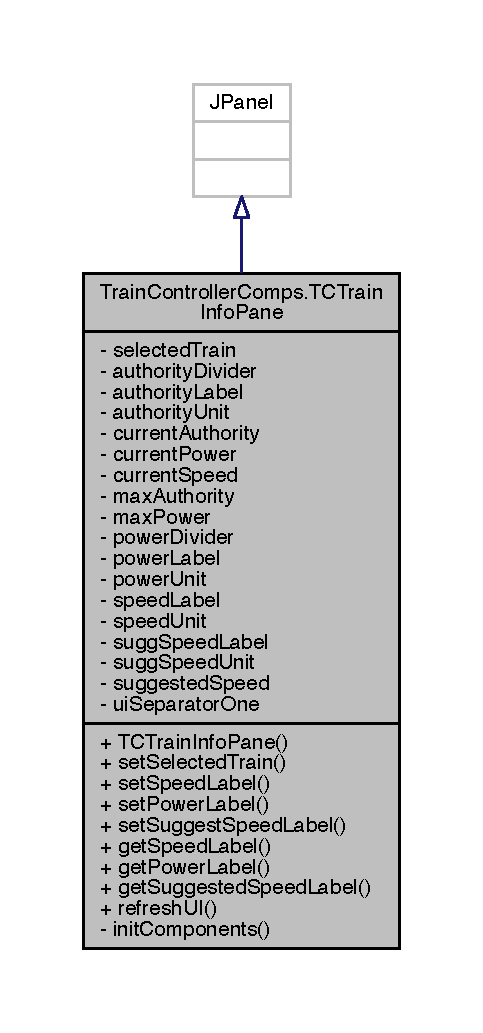
\includegraphics[width=232pt]{classTrainControllerComps_1_1TCTrainInfoPane__inherit__graph}
\end{center}
\end{figure}


Collaboration diagram for Train\+Controller\+Comps.\+T\+C\+Train\+Info\+Pane\+:
\nopagebreak
\begin{figure}[H]
\begin{center}
\leavevmode
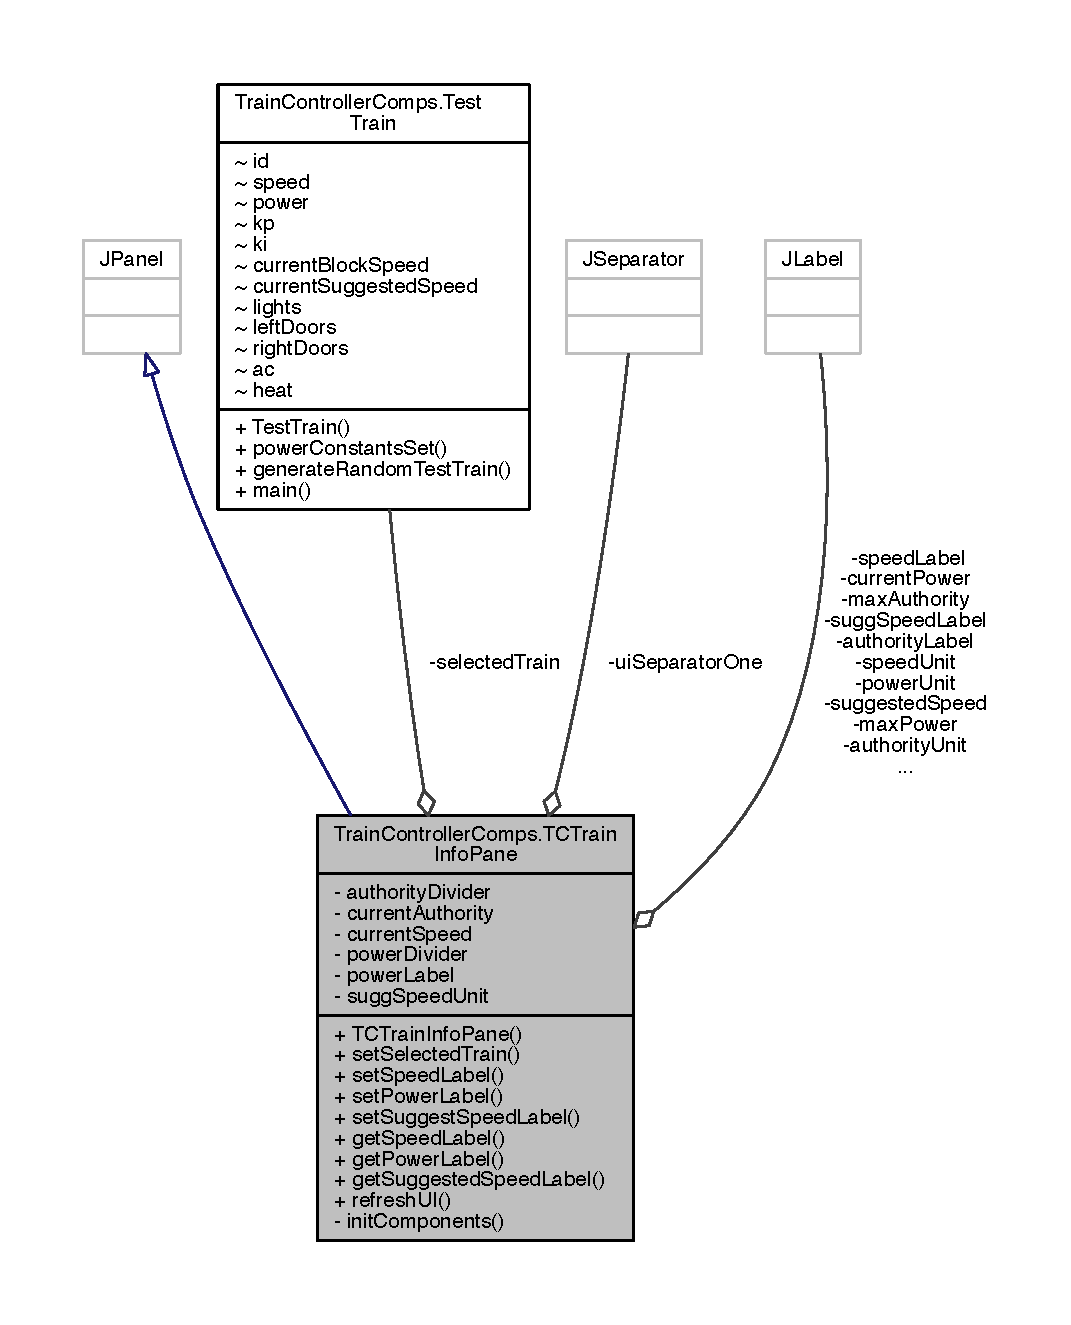
\includegraphics[width=350pt]{classTrainControllerComps_1_1TCTrainInfoPane__coll__graph}
\end{center}
\end{figure}
\subsection*{Public Member Functions}
\begin{DoxyCompactItemize}
\item 
\hyperlink{classTrainControllerComps_1_1TCTrainInfoPane_adb9f574b995a252e6e1fc1ee73402801}{T\+C\+Train\+Info\+Pane} ()
\begin{DoxyCompactList}\small\item\em Constructor for creating a \hyperlink{classTrainControllerComps_1_1TCTrainInfoPane}{T\+C\+Train\+Info\+Pane} object with no selected train. \end{DoxyCompactList}\item 
void \hyperlink{classTrainControllerComps_1_1TCTrainInfoPane_aa3515128954b5bf339df6926d29e0424}{set\+Selected\+Train} (\hyperlink{classTrainControllerComps_1_1TestTrain}{Test\+Train} \hyperlink{classtrain}{train})
\begin{DoxyCompactList}\small\item\em Sets the train whose info to display to the user. \end{DoxyCompactList}\item 
void \hyperlink{classTrainControllerComps_1_1TCTrainInfoPane_aaa8d8d930a3d0cce4286f44e0600b820}{set\+Speed\+Label} (double speed)
\begin{DoxyCompactList}\small\item\em Sets the speed the train is currently going. \end{DoxyCompactList}\item 
void \hyperlink{classTrainControllerComps_1_1TCTrainInfoPane_a3ec6d080c4a75c031678b8d4620153d0}{set\+Power\+Label} (double power)
\begin{DoxyCompactList}\small\item\em Sets the power the train is currently producing. \end{DoxyCompactList}\item 
void \hyperlink{classTrainControllerComps_1_1TCTrainInfoPane_ab2965544592b8ee90697d9ad4c0d00de}{set\+Suggest\+Speed\+Label} (double sugg\+Speed)
\begin{DoxyCompactList}\small\item\em Sets the suggested speed for the train. \end{DoxyCompactList}\item 
String \hyperlink{classTrainControllerComps_1_1TCTrainInfoPane_a9146b41e4efe422586c69624f6e16e2f}{get\+Speed\+Label} ()
\begin{DoxyCompactList}\small\item\em Retrieves the speed the train is going from the speed label. \end{DoxyCompactList}\item 
String \hyperlink{classTrainControllerComps_1_1TCTrainInfoPane_a5c3ebdfe9c6a2d7357a460475e9fd55c}{get\+Power\+Label} ()
\begin{DoxyCompactList}\small\item\em Retrieves the power the train is applying from the power label. \end{DoxyCompactList}\item 
String \hyperlink{classTrainControllerComps_1_1TCTrainInfoPane_ae8aae7010c588984b4bdc7f1422e1d3e}{get\+Suggested\+Speed\+Label} ()
\begin{DoxyCompactList}\small\item\em Retrieves the suggested speed of the train from the suggested speed label. \end{DoxyCompactList}\item 
void \hyperlink{classTrainControllerComps_1_1TCTrainInfoPane_a82dcf410364f2712296b1505d6175b3a}{refresh\+UI} ()
\begin{DoxyCompactList}\small\item\em Updates the labels with the information based on the selected train. \end{DoxyCompactList}\end{DoxyCompactItemize}
\subsection*{Private Member Functions}
\begin{DoxyCompactItemize}
\item 
void \hyperlink{classTrainControllerComps_1_1TCTrainInfoPane_a875ccb16a90d10cc999f0c274824778e}{init\+Components} ()
\begin{DoxyCompactList}\small\item\em This method is called from within the constructor to initialize the form. \end{DoxyCompactList}\end{DoxyCompactItemize}
\subsection*{Private Attributes}
\begin{DoxyCompactItemize}
\item 
\hyperlink{classTrainControllerComps_1_1TestTrain}{Test\+Train} \hyperlink{classTrainControllerComps_1_1TCTrainInfoPane_ae4816b54fe2e5f0e0d81d1dd3ab03c30}{selected\+Train}
\begin{DoxyCompactList}\small\item\em The train used to update the UI based on its information. \end{DoxyCompactList}\item 
javax.\+swing.\+J\+Label \hyperlink{classTrainControllerComps_1_1TCTrainInfoPane_a733e39ce58b6d8707aeadf9ba081945d}{authority\+Divider}
\item 
javax.\+swing.\+J\+Label \hyperlink{classTrainControllerComps_1_1TCTrainInfoPane_ad3834c784cc325e3d9a760e206926bbe}{authority\+Label}
\item 
javax.\+swing.\+J\+Label \hyperlink{classTrainControllerComps_1_1TCTrainInfoPane_a85f02470ad2e701f9b3a4d59a238621d}{authority\+Unit}
\item 
javax.\+swing.\+J\+Label \hyperlink{classTrainControllerComps_1_1TCTrainInfoPane_acf3b7428f9c5c582e82d08e0bdba9d6f}{current\+Authority}
\item 
javax.\+swing.\+J\+Label \hyperlink{classTrainControllerComps_1_1TCTrainInfoPane_ad703e120928f8a764cbca4941c7ea430}{current\+Power}
\item 
javax.\+swing.\+J\+Label \hyperlink{classTrainControllerComps_1_1TCTrainInfoPane_a23261167c5a4108920049381ef5a9149}{current\+Speed}
\item 
javax.\+swing.\+J\+Label \hyperlink{classTrainControllerComps_1_1TCTrainInfoPane_aad833d5c75b6a626a8bb4e58f396eb92}{max\+Authority}
\item 
javax.\+swing.\+J\+Label \hyperlink{classTrainControllerComps_1_1TCTrainInfoPane_a18fc7fcbd582f9aea6b9afba7a7f1eb1}{max\+Power}
\item 
javax.\+swing.\+J\+Label \hyperlink{classTrainControllerComps_1_1TCTrainInfoPane_ac969dbb23d7883d2aae970c6b564790b}{power\+Divider}
\item 
javax.\+swing.\+J\+Label \hyperlink{classTrainControllerComps_1_1TCTrainInfoPane_a22c155dab57f64948d34bd5f8457eeed}{power\+Label}
\item 
javax.\+swing.\+J\+Label \hyperlink{classTrainControllerComps_1_1TCTrainInfoPane_a56aeb864b027cbcdd3981a4c73159f0d}{power\+Unit}
\item 
javax.\+swing.\+J\+Label \hyperlink{classTrainControllerComps_1_1TCTrainInfoPane_a3ad3cc96e1a10e25ccec0524462cd1ec}{speed\+Label}
\item 
javax.\+swing.\+J\+Label \hyperlink{classTrainControllerComps_1_1TCTrainInfoPane_a8f20fe11080e6925e462f0876601a6da}{speed\+Unit}
\item 
javax.\+swing.\+J\+Label \hyperlink{classTrainControllerComps_1_1TCTrainInfoPane_a93e0c69b22525e4d1f97e3f725f7c8a1}{sugg\+Speed\+Label}
\item 
javax.\+swing.\+J\+Label \hyperlink{classTrainControllerComps_1_1TCTrainInfoPane_a595ef0eaa17bbdfc0c1f08a4850c8a9e}{sugg\+Speed\+Unit}
\item 
javax.\+swing.\+J\+Label \hyperlink{classTrainControllerComps_1_1TCTrainInfoPane_abc7d24f507a112d03fe323f853b9d4d3}{suggested\+Speed}
\item 
javax.\+swing.\+J\+Separator \hyperlink{classTrainControllerComps_1_1TCTrainInfoPane_a97285213bfc29bdda84e53054b83ed7b}{ui\+Separator\+One}
\end{DoxyCompactItemize}


\subsection{Detailed Description}
A component of the Train Controller responsible for the selected train\textquotesingle{}s speed, power, authority, and suggested speed. 

This class collaborates with the Train Controller and Train class.

\begin{DoxyAuthor}{Author}
Andrew Lendacky 
\end{DoxyAuthor}


\subsection{Constructor \& Destructor Documentation}
\mbox{\Hypertarget{classTrainControllerComps_1_1TCTrainInfoPane_adb9f574b995a252e6e1fc1ee73402801}\label{classTrainControllerComps_1_1TCTrainInfoPane_adb9f574b995a252e6e1fc1ee73402801}} 
\index{Train\+Controller\+Comps\+::\+T\+C\+Train\+Info\+Pane@{Train\+Controller\+Comps\+::\+T\+C\+Train\+Info\+Pane}!T\+C\+Train\+Info\+Pane@{T\+C\+Train\+Info\+Pane}}
\index{T\+C\+Train\+Info\+Pane@{T\+C\+Train\+Info\+Pane}!Train\+Controller\+Comps\+::\+T\+C\+Train\+Info\+Pane@{Train\+Controller\+Comps\+::\+T\+C\+Train\+Info\+Pane}}
\subsubsection{\texorpdfstring{T\+C\+Train\+Info\+Pane()}{TCTrainInfoPane()}}
{\footnotesize\ttfamily Train\+Controller\+Comps.\+T\+C\+Train\+Info\+Pane.\+T\+C\+Train\+Info\+Pane (\begin{DoxyParamCaption}{ }\end{DoxyParamCaption})}



Constructor for creating a \hyperlink{classTrainControllerComps_1_1TCTrainInfoPane}{T\+C\+Train\+Info\+Pane} object with no selected train. 

The selected train must be set by the Train Controller before being used. 

\subsection{Member Function Documentation}
\mbox{\Hypertarget{classTrainControllerComps_1_1TCTrainInfoPane_a5c3ebdfe9c6a2d7357a460475e9fd55c}\label{classTrainControllerComps_1_1TCTrainInfoPane_a5c3ebdfe9c6a2d7357a460475e9fd55c}} 
\index{Train\+Controller\+Comps\+::\+T\+C\+Train\+Info\+Pane@{Train\+Controller\+Comps\+::\+T\+C\+Train\+Info\+Pane}!get\+Power\+Label@{get\+Power\+Label}}
\index{get\+Power\+Label@{get\+Power\+Label}!Train\+Controller\+Comps\+::\+T\+C\+Train\+Info\+Pane@{Train\+Controller\+Comps\+::\+T\+C\+Train\+Info\+Pane}}
\subsubsection{\texorpdfstring{get\+Power\+Label()}{getPowerLabel()}}
{\footnotesize\ttfamily String Train\+Controller\+Comps.\+T\+C\+Train\+Info\+Pane.\+get\+Power\+Label (\begin{DoxyParamCaption}{ }\end{DoxyParamCaption})}



Retrieves the power the train is applying from the power label. 

\begin{DoxyReturn}{Returns}
returns the text corresponding to the power of the train from the power label. 
\end{DoxyReturn}
\mbox{\Hypertarget{classTrainControllerComps_1_1TCTrainInfoPane_a9146b41e4efe422586c69624f6e16e2f}\label{classTrainControllerComps_1_1TCTrainInfoPane_a9146b41e4efe422586c69624f6e16e2f}} 
\index{Train\+Controller\+Comps\+::\+T\+C\+Train\+Info\+Pane@{Train\+Controller\+Comps\+::\+T\+C\+Train\+Info\+Pane}!get\+Speed\+Label@{get\+Speed\+Label}}
\index{get\+Speed\+Label@{get\+Speed\+Label}!Train\+Controller\+Comps\+::\+T\+C\+Train\+Info\+Pane@{Train\+Controller\+Comps\+::\+T\+C\+Train\+Info\+Pane}}
\subsubsection{\texorpdfstring{get\+Speed\+Label()}{getSpeedLabel()}}
{\footnotesize\ttfamily String Train\+Controller\+Comps.\+T\+C\+Train\+Info\+Pane.\+get\+Speed\+Label (\begin{DoxyParamCaption}{ }\end{DoxyParamCaption})}



Retrieves the speed the train is going from the speed label. 

\begin{DoxyReturn}{Returns}
returns the text corresponding to the speed of the train from the speed label. 
\end{DoxyReturn}
\mbox{\Hypertarget{classTrainControllerComps_1_1TCTrainInfoPane_ae8aae7010c588984b4bdc7f1422e1d3e}\label{classTrainControllerComps_1_1TCTrainInfoPane_ae8aae7010c588984b4bdc7f1422e1d3e}} 
\index{Train\+Controller\+Comps\+::\+T\+C\+Train\+Info\+Pane@{Train\+Controller\+Comps\+::\+T\+C\+Train\+Info\+Pane}!get\+Suggested\+Speed\+Label@{get\+Suggested\+Speed\+Label}}
\index{get\+Suggested\+Speed\+Label@{get\+Suggested\+Speed\+Label}!Train\+Controller\+Comps\+::\+T\+C\+Train\+Info\+Pane@{Train\+Controller\+Comps\+::\+T\+C\+Train\+Info\+Pane}}
\subsubsection{\texorpdfstring{get\+Suggested\+Speed\+Label()}{getSuggestedSpeedLabel()}}
{\footnotesize\ttfamily String Train\+Controller\+Comps.\+T\+C\+Train\+Info\+Pane.\+get\+Suggested\+Speed\+Label (\begin{DoxyParamCaption}{ }\end{DoxyParamCaption})}



Retrieves the suggested speed of the train from the suggested speed label. 

\begin{DoxyReturn}{Returns}
returns the text corresponding to the suggested speed of the train from the suggested speed label. 
\end{DoxyReturn}
\mbox{\Hypertarget{classTrainControllerComps_1_1TCTrainInfoPane_a875ccb16a90d10cc999f0c274824778e}\label{classTrainControllerComps_1_1TCTrainInfoPane_a875ccb16a90d10cc999f0c274824778e}} 
\index{Train\+Controller\+Comps\+::\+T\+C\+Train\+Info\+Pane@{Train\+Controller\+Comps\+::\+T\+C\+Train\+Info\+Pane}!init\+Components@{init\+Components}}
\index{init\+Components@{init\+Components}!Train\+Controller\+Comps\+::\+T\+C\+Train\+Info\+Pane@{Train\+Controller\+Comps\+::\+T\+C\+Train\+Info\+Pane}}
\subsubsection{\texorpdfstring{init\+Components()}{initComponents()}}
{\footnotesize\ttfamily void Train\+Controller\+Comps.\+T\+C\+Train\+Info\+Pane.\+init\+Components (\begin{DoxyParamCaption}{ }\end{DoxyParamCaption})\hspace{0.3cm}{\ttfamily [private]}}



This method is called from within the constructor to initialize the form. 

W\+A\+R\+N\+I\+NG\+: Do N\+OT modify this code. The content of this method is always regenerated by the Form Editor. \mbox{\Hypertarget{classTrainControllerComps_1_1TCTrainInfoPane_a82dcf410364f2712296b1505d6175b3a}\label{classTrainControllerComps_1_1TCTrainInfoPane_a82dcf410364f2712296b1505d6175b3a}} 
\index{Train\+Controller\+Comps\+::\+T\+C\+Train\+Info\+Pane@{Train\+Controller\+Comps\+::\+T\+C\+Train\+Info\+Pane}!refresh\+UI@{refresh\+UI}}
\index{refresh\+UI@{refresh\+UI}!Train\+Controller\+Comps\+::\+T\+C\+Train\+Info\+Pane@{Train\+Controller\+Comps\+::\+T\+C\+Train\+Info\+Pane}}
\subsubsection{\texorpdfstring{refresh\+U\+I()}{refreshUI()}}
{\footnotesize\ttfamily void Train\+Controller\+Comps.\+T\+C\+Train\+Info\+Pane.\+refresh\+UI (\begin{DoxyParamCaption}{ }\end{DoxyParamCaption})}



Updates the labels with the information based on the selected train. 

\mbox{\Hypertarget{classTrainControllerComps_1_1TCTrainInfoPane_a3ec6d080c4a75c031678b8d4620153d0}\label{classTrainControllerComps_1_1TCTrainInfoPane_a3ec6d080c4a75c031678b8d4620153d0}} 
\index{Train\+Controller\+Comps\+::\+T\+C\+Train\+Info\+Pane@{Train\+Controller\+Comps\+::\+T\+C\+Train\+Info\+Pane}!set\+Power\+Label@{set\+Power\+Label}}
\index{set\+Power\+Label@{set\+Power\+Label}!Train\+Controller\+Comps\+::\+T\+C\+Train\+Info\+Pane@{Train\+Controller\+Comps\+::\+T\+C\+Train\+Info\+Pane}}
\subsubsection{\texorpdfstring{set\+Power\+Label()}{setPowerLabel()}}
{\footnotesize\ttfamily void Train\+Controller\+Comps.\+T\+C\+Train\+Info\+Pane.\+set\+Power\+Label (\begin{DoxyParamCaption}\item[{double}]{power }\end{DoxyParamCaption})}



Sets the power the train is currently producing. 


\begin{DoxyParams}{Parameters}
{\em power} & the power the train is producing. \\
\hline
\end{DoxyParams}
\mbox{\Hypertarget{classTrainControllerComps_1_1TCTrainInfoPane_aa3515128954b5bf339df6926d29e0424}\label{classTrainControllerComps_1_1TCTrainInfoPane_aa3515128954b5bf339df6926d29e0424}} 
\index{Train\+Controller\+Comps\+::\+T\+C\+Train\+Info\+Pane@{Train\+Controller\+Comps\+::\+T\+C\+Train\+Info\+Pane}!set\+Selected\+Train@{set\+Selected\+Train}}
\index{set\+Selected\+Train@{set\+Selected\+Train}!Train\+Controller\+Comps\+::\+T\+C\+Train\+Info\+Pane@{Train\+Controller\+Comps\+::\+T\+C\+Train\+Info\+Pane}}
\subsubsection{\texorpdfstring{set\+Selected\+Train()}{setSelectedTrain()}}
{\footnotesize\ttfamily void Train\+Controller\+Comps.\+T\+C\+Train\+Info\+Pane.\+set\+Selected\+Train (\begin{DoxyParamCaption}\item[{\hyperlink{classTrainControllerComps_1_1TestTrain}{Test\+Train}}]{train }\end{DoxyParamCaption})}



Sets the train whose info to display to the user. 


\begin{DoxyParams}{Parameters}
{\em train} & the train controlled by the Train Controller. \\
\hline
\end{DoxyParams}
\mbox{\Hypertarget{classTrainControllerComps_1_1TCTrainInfoPane_aaa8d8d930a3d0cce4286f44e0600b820}\label{classTrainControllerComps_1_1TCTrainInfoPane_aaa8d8d930a3d0cce4286f44e0600b820}} 
\index{Train\+Controller\+Comps\+::\+T\+C\+Train\+Info\+Pane@{Train\+Controller\+Comps\+::\+T\+C\+Train\+Info\+Pane}!set\+Speed\+Label@{set\+Speed\+Label}}
\index{set\+Speed\+Label@{set\+Speed\+Label}!Train\+Controller\+Comps\+::\+T\+C\+Train\+Info\+Pane@{Train\+Controller\+Comps\+::\+T\+C\+Train\+Info\+Pane}}
\subsubsection{\texorpdfstring{set\+Speed\+Label()}{setSpeedLabel()}}
{\footnotesize\ttfamily void Train\+Controller\+Comps.\+T\+C\+Train\+Info\+Pane.\+set\+Speed\+Label (\begin{DoxyParamCaption}\item[{double}]{speed }\end{DoxyParamCaption})}



Sets the speed the train is currently going. 


\begin{DoxyParams}{Parameters}
{\em speed} & the speed the train is going. \\
\hline
\end{DoxyParams}
\mbox{\Hypertarget{classTrainControllerComps_1_1TCTrainInfoPane_ab2965544592b8ee90697d9ad4c0d00de}\label{classTrainControllerComps_1_1TCTrainInfoPane_ab2965544592b8ee90697d9ad4c0d00de}} 
\index{Train\+Controller\+Comps\+::\+T\+C\+Train\+Info\+Pane@{Train\+Controller\+Comps\+::\+T\+C\+Train\+Info\+Pane}!set\+Suggest\+Speed\+Label@{set\+Suggest\+Speed\+Label}}
\index{set\+Suggest\+Speed\+Label@{set\+Suggest\+Speed\+Label}!Train\+Controller\+Comps\+::\+T\+C\+Train\+Info\+Pane@{Train\+Controller\+Comps\+::\+T\+C\+Train\+Info\+Pane}}
\subsubsection{\texorpdfstring{set\+Suggest\+Speed\+Label()}{setSuggestSpeedLabel()}}
{\footnotesize\ttfamily void Train\+Controller\+Comps.\+T\+C\+Train\+Info\+Pane.\+set\+Suggest\+Speed\+Label (\begin{DoxyParamCaption}\item[{double}]{sugg\+Speed }\end{DoxyParamCaption})}



Sets the suggested speed for the train. 

This speed comes from the C\+TC.


\begin{DoxyParams}{Parameters}
{\em sugg\+Speed} & the suggested speed for the train. \\
\hline
\end{DoxyParams}


\subsection{Member Data Documentation}
\mbox{\Hypertarget{classTrainControllerComps_1_1TCTrainInfoPane_a733e39ce58b6d8707aeadf9ba081945d}\label{classTrainControllerComps_1_1TCTrainInfoPane_a733e39ce58b6d8707aeadf9ba081945d}} 
\index{Train\+Controller\+Comps\+::\+T\+C\+Train\+Info\+Pane@{Train\+Controller\+Comps\+::\+T\+C\+Train\+Info\+Pane}!authority\+Divider@{authority\+Divider}}
\index{authority\+Divider@{authority\+Divider}!Train\+Controller\+Comps\+::\+T\+C\+Train\+Info\+Pane@{Train\+Controller\+Comps\+::\+T\+C\+Train\+Info\+Pane}}
\subsubsection{\texorpdfstring{authority\+Divider}{authorityDivider}}
{\footnotesize\ttfamily javax.\+swing.\+J\+Label Train\+Controller\+Comps.\+T\+C\+Train\+Info\+Pane.\+authority\+Divider\hspace{0.3cm}{\ttfamily [private]}}

\mbox{\Hypertarget{classTrainControllerComps_1_1TCTrainInfoPane_ad3834c784cc325e3d9a760e206926bbe}\label{classTrainControllerComps_1_1TCTrainInfoPane_ad3834c784cc325e3d9a760e206926bbe}} 
\index{Train\+Controller\+Comps\+::\+T\+C\+Train\+Info\+Pane@{Train\+Controller\+Comps\+::\+T\+C\+Train\+Info\+Pane}!authority\+Label@{authority\+Label}}
\index{authority\+Label@{authority\+Label}!Train\+Controller\+Comps\+::\+T\+C\+Train\+Info\+Pane@{Train\+Controller\+Comps\+::\+T\+C\+Train\+Info\+Pane}}
\subsubsection{\texorpdfstring{authority\+Label}{authorityLabel}}
{\footnotesize\ttfamily javax.\+swing.\+J\+Label Train\+Controller\+Comps.\+T\+C\+Train\+Info\+Pane.\+authority\+Label\hspace{0.3cm}{\ttfamily [private]}}

\mbox{\Hypertarget{classTrainControllerComps_1_1TCTrainInfoPane_a85f02470ad2e701f9b3a4d59a238621d}\label{classTrainControllerComps_1_1TCTrainInfoPane_a85f02470ad2e701f9b3a4d59a238621d}} 
\index{Train\+Controller\+Comps\+::\+T\+C\+Train\+Info\+Pane@{Train\+Controller\+Comps\+::\+T\+C\+Train\+Info\+Pane}!authority\+Unit@{authority\+Unit}}
\index{authority\+Unit@{authority\+Unit}!Train\+Controller\+Comps\+::\+T\+C\+Train\+Info\+Pane@{Train\+Controller\+Comps\+::\+T\+C\+Train\+Info\+Pane}}
\subsubsection{\texorpdfstring{authority\+Unit}{authorityUnit}}
{\footnotesize\ttfamily javax.\+swing.\+J\+Label Train\+Controller\+Comps.\+T\+C\+Train\+Info\+Pane.\+authority\+Unit\hspace{0.3cm}{\ttfamily [private]}}

\mbox{\Hypertarget{classTrainControllerComps_1_1TCTrainInfoPane_acf3b7428f9c5c582e82d08e0bdba9d6f}\label{classTrainControllerComps_1_1TCTrainInfoPane_acf3b7428f9c5c582e82d08e0bdba9d6f}} 
\index{Train\+Controller\+Comps\+::\+T\+C\+Train\+Info\+Pane@{Train\+Controller\+Comps\+::\+T\+C\+Train\+Info\+Pane}!current\+Authority@{current\+Authority}}
\index{current\+Authority@{current\+Authority}!Train\+Controller\+Comps\+::\+T\+C\+Train\+Info\+Pane@{Train\+Controller\+Comps\+::\+T\+C\+Train\+Info\+Pane}}
\subsubsection{\texorpdfstring{current\+Authority}{currentAuthority}}
{\footnotesize\ttfamily javax.\+swing.\+J\+Label Train\+Controller\+Comps.\+T\+C\+Train\+Info\+Pane.\+current\+Authority\hspace{0.3cm}{\ttfamily [private]}}

\mbox{\Hypertarget{classTrainControllerComps_1_1TCTrainInfoPane_ad703e120928f8a764cbca4941c7ea430}\label{classTrainControllerComps_1_1TCTrainInfoPane_ad703e120928f8a764cbca4941c7ea430}} 
\index{Train\+Controller\+Comps\+::\+T\+C\+Train\+Info\+Pane@{Train\+Controller\+Comps\+::\+T\+C\+Train\+Info\+Pane}!current\+Power@{current\+Power}}
\index{current\+Power@{current\+Power}!Train\+Controller\+Comps\+::\+T\+C\+Train\+Info\+Pane@{Train\+Controller\+Comps\+::\+T\+C\+Train\+Info\+Pane}}
\subsubsection{\texorpdfstring{current\+Power}{currentPower}}
{\footnotesize\ttfamily javax.\+swing.\+J\+Label Train\+Controller\+Comps.\+T\+C\+Train\+Info\+Pane.\+current\+Power\hspace{0.3cm}{\ttfamily [private]}}

\mbox{\Hypertarget{classTrainControllerComps_1_1TCTrainInfoPane_a23261167c5a4108920049381ef5a9149}\label{classTrainControllerComps_1_1TCTrainInfoPane_a23261167c5a4108920049381ef5a9149}} 
\index{Train\+Controller\+Comps\+::\+T\+C\+Train\+Info\+Pane@{Train\+Controller\+Comps\+::\+T\+C\+Train\+Info\+Pane}!current\+Speed@{current\+Speed}}
\index{current\+Speed@{current\+Speed}!Train\+Controller\+Comps\+::\+T\+C\+Train\+Info\+Pane@{Train\+Controller\+Comps\+::\+T\+C\+Train\+Info\+Pane}}
\subsubsection{\texorpdfstring{current\+Speed}{currentSpeed}}
{\footnotesize\ttfamily javax.\+swing.\+J\+Label Train\+Controller\+Comps.\+T\+C\+Train\+Info\+Pane.\+current\+Speed\hspace{0.3cm}{\ttfamily [private]}}

\mbox{\Hypertarget{classTrainControllerComps_1_1TCTrainInfoPane_aad833d5c75b6a626a8bb4e58f396eb92}\label{classTrainControllerComps_1_1TCTrainInfoPane_aad833d5c75b6a626a8bb4e58f396eb92}} 
\index{Train\+Controller\+Comps\+::\+T\+C\+Train\+Info\+Pane@{Train\+Controller\+Comps\+::\+T\+C\+Train\+Info\+Pane}!max\+Authority@{max\+Authority}}
\index{max\+Authority@{max\+Authority}!Train\+Controller\+Comps\+::\+T\+C\+Train\+Info\+Pane@{Train\+Controller\+Comps\+::\+T\+C\+Train\+Info\+Pane}}
\subsubsection{\texorpdfstring{max\+Authority}{maxAuthority}}
{\footnotesize\ttfamily javax.\+swing.\+J\+Label Train\+Controller\+Comps.\+T\+C\+Train\+Info\+Pane.\+max\+Authority\hspace{0.3cm}{\ttfamily [private]}}

\mbox{\Hypertarget{classTrainControllerComps_1_1TCTrainInfoPane_a18fc7fcbd582f9aea6b9afba7a7f1eb1}\label{classTrainControllerComps_1_1TCTrainInfoPane_a18fc7fcbd582f9aea6b9afba7a7f1eb1}} 
\index{Train\+Controller\+Comps\+::\+T\+C\+Train\+Info\+Pane@{Train\+Controller\+Comps\+::\+T\+C\+Train\+Info\+Pane}!max\+Power@{max\+Power}}
\index{max\+Power@{max\+Power}!Train\+Controller\+Comps\+::\+T\+C\+Train\+Info\+Pane@{Train\+Controller\+Comps\+::\+T\+C\+Train\+Info\+Pane}}
\subsubsection{\texorpdfstring{max\+Power}{maxPower}}
{\footnotesize\ttfamily javax.\+swing.\+J\+Label Train\+Controller\+Comps.\+T\+C\+Train\+Info\+Pane.\+max\+Power\hspace{0.3cm}{\ttfamily [private]}}

\mbox{\Hypertarget{classTrainControllerComps_1_1TCTrainInfoPane_ac969dbb23d7883d2aae970c6b564790b}\label{classTrainControllerComps_1_1TCTrainInfoPane_ac969dbb23d7883d2aae970c6b564790b}} 
\index{Train\+Controller\+Comps\+::\+T\+C\+Train\+Info\+Pane@{Train\+Controller\+Comps\+::\+T\+C\+Train\+Info\+Pane}!power\+Divider@{power\+Divider}}
\index{power\+Divider@{power\+Divider}!Train\+Controller\+Comps\+::\+T\+C\+Train\+Info\+Pane@{Train\+Controller\+Comps\+::\+T\+C\+Train\+Info\+Pane}}
\subsubsection{\texorpdfstring{power\+Divider}{powerDivider}}
{\footnotesize\ttfamily javax.\+swing.\+J\+Label Train\+Controller\+Comps.\+T\+C\+Train\+Info\+Pane.\+power\+Divider\hspace{0.3cm}{\ttfamily [private]}}

\mbox{\Hypertarget{classTrainControllerComps_1_1TCTrainInfoPane_a22c155dab57f64948d34bd5f8457eeed}\label{classTrainControllerComps_1_1TCTrainInfoPane_a22c155dab57f64948d34bd5f8457eeed}} 
\index{Train\+Controller\+Comps\+::\+T\+C\+Train\+Info\+Pane@{Train\+Controller\+Comps\+::\+T\+C\+Train\+Info\+Pane}!power\+Label@{power\+Label}}
\index{power\+Label@{power\+Label}!Train\+Controller\+Comps\+::\+T\+C\+Train\+Info\+Pane@{Train\+Controller\+Comps\+::\+T\+C\+Train\+Info\+Pane}}
\subsubsection{\texorpdfstring{power\+Label}{powerLabel}}
{\footnotesize\ttfamily javax.\+swing.\+J\+Label Train\+Controller\+Comps.\+T\+C\+Train\+Info\+Pane.\+power\+Label\hspace{0.3cm}{\ttfamily [private]}}

\mbox{\Hypertarget{classTrainControllerComps_1_1TCTrainInfoPane_a56aeb864b027cbcdd3981a4c73159f0d}\label{classTrainControllerComps_1_1TCTrainInfoPane_a56aeb864b027cbcdd3981a4c73159f0d}} 
\index{Train\+Controller\+Comps\+::\+T\+C\+Train\+Info\+Pane@{Train\+Controller\+Comps\+::\+T\+C\+Train\+Info\+Pane}!power\+Unit@{power\+Unit}}
\index{power\+Unit@{power\+Unit}!Train\+Controller\+Comps\+::\+T\+C\+Train\+Info\+Pane@{Train\+Controller\+Comps\+::\+T\+C\+Train\+Info\+Pane}}
\subsubsection{\texorpdfstring{power\+Unit}{powerUnit}}
{\footnotesize\ttfamily javax.\+swing.\+J\+Label Train\+Controller\+Comps.\+T\+C\+Train\+Info\+Pane.\+power\+Unit\hspace{0.3cm}{\ttfamily [private]}}

\mbox{\Hypertarget{classTrainControllerComps_1_1TCTrainInfoPane_ae4816b54fe2e5f0e0d81d1dd3ab03c30}\label{classTrainControllerComps_1_1TCTrainInfoPane_ae4816b54fe2e5f0e0d81d1dd3ab03c30}} 
\index{Train\+Controller\+Comps\+::\+T\+C\+Train\+Info\+Pane@{Train\+Controller\+Comps\+::\+T\+C\+Train\+Info\+Pane}!selected\+Train@{selected\+Train}}
\index{selected\+Train@{selected\+Train}!Train\+Controller\+Comps\+::\+T\+C\+Train\+Info\+Pane@{Train\+Controller\+Comps\+::\+T\+C\+Train\+Info\+Pane}}
\subsubsection{\texorpdfstring{selected\+Train}{selectedTrain}}
{\footnotesize\ttfamily \hyperlink{classTrainControllerComps_1_1TestTrain}{Test\+Train} Train\+Controller\+Comps.\+T\+C\+Train\+Info\+Pane.\+selected\+Train\hspace{0.3cm}{\ttfamily [private]}}



The train used to update the UI based on its information. 

\mbox{\Hypertarget{classTrainControllerComps_1_1TCTrainInfoPane_a3ad3cc96e1a10e25ccec0524462cd1ec}\label{classTrainControllerComps_1_1TCTrainInfoPane_a3ad3cc96e1a10e25ccec0524462cd1ec}} 
\index{Train\+Controller\+Comps\+::\+T\+C\+Train\+Info\+Pane@{Train\+Controller\+Comps\+::\+T\+C\+Train\+Info\+Pane}!speed\+Label@{speed\+Label}}
\index{speed\+Label@{speed\+Label}!Train\+Controller\+Comps\+::\+T\+C\+Train\+Info\+Pane@{Train\+Controller\+Comps\+::\+T\+C\+Train\+Info\+Pane}}
\subsubsection{\texorpdfstring{speed\+Label}{speedLabel}}
{\footnotesize\ttfamily javax.\+swing.\+J\+Label Train\+Controller\+Comps.\+T\+C\+Train\+Info\+Pane.\+speed\+Label\hspace{0.3cm}{\ttfamily [private]}}

\mbox{\Hypertarget{classTrainControllerComps_1_1TCTrainInfoPane_a8f20fe11080e6925e462f0876601a6da}\label{classTrainControllerComps_1_1TCTrainInfoPane_a8f20fe11080e6925e462f0876601a6da}} 
\index{Train\+Controller\+Comps\+::\+T\+C\+Train\+Info\+Pane@{Train\+Controller\+Comps\+::\+T\+C\+Train\+Info\+Pane}!speed\+Unit@{speed\+Unit}}
\index{speed\+Unit@{speed\+Unit}!Train\+Controller\+Comps\+::\+T\+C\+Train\+Info\+Pane@{Train\+Controller\+Comps\+::\+T\+C\+Train\+Info\+Pane}}
\subsubsection{\texorpdfstring{speed\+Unit}{speedUnit}}
{\footnotesize\ttfamily javax.\+swing.\+J\+Label Train\+Controller\+Comps.\+T\+C\+Train\+Info\+Pane.\+speed\+Unit\hspace{0.3cm}{\ttfamily [private]}}

\mbox{\Hypertarget{classTrainControllerComps_1_1TCTrainInfoPane_abc7d24f507a112d03fe323f853b9d4d3}\label{classTrainControllerComps_1_1TCTrainInfoPane_abc7d24f507a112d03fe323f853b9d4d3}} 
\index{Train\+Controller\+Comps\+::\+T\+C\+Train\+Info\+Pane@{Train\+Controller\+Comps\+::\+T\+C\+Train\+Info\+Pane}!suggested\+Speed@{suggested\+Speed}}
\index{suggested\+Speed@{suggested\+Speed}!Train\+Controller\+Comps\+::\+T\+C\+Train\+Info\+Pane@{Train\+Controller\+Comps\+::\+T\+C\+Train\+Info\+Pane}}
\subsubsection{\texorpdfstring{suggested\+Speed}{suggestedSpeed}}
{\footnotesize\ttfamily javax.\+swing.\+J\+Label Train\+Controller\+Comps.\+T\+C\+Train\+Info\+Pane.\+suggested\+Speed\hspace{0.3cm}{\ttfamily [private]}}

\mbox{\Hypertarget{classTrainControllerComps_1_1TCTrainInfoPane_a93e0c69b22525e4d1f97e3f725f7c8a1}\label{classTrainControllerComps_1_1TCTrainInfoPane_a93e0c69b22525e4d1f97e3f725f7c8a1}} 
\index{Train\+Controller\+Comps\+::\+T\+C\+Train\+Info\+Pane@{Train\+Controller\+Comps\+::\+T\+C\+Train\+Info\+Pane}!sugg\+Speed\+Label@{sugg\+Speed\+Label}}
\index{sugg\+Speed\+Label@{sugg\+Speed\+Label}!Train\+Controller\+Comps\+::\+T\+C\+Train\+Info\+Pane@{Train\+Controller\+Comps\+::\+T\+C\+Train\+Info\+Pane}}
\subsubsection{\texorpdfstring{sugg\+Speed\+Label}{suggSpeedLabel}}
{\footnotesize\ttfamily javax.\+swing.\+J\+Label Train\+Controller\+Comps.\+T\+C\+Train\+Info\+Pane.\+sugg\+Speed\+Label\hspace{0.3cm}{\ttfamily [private]}}

\mbox{\Hypertarget{classTrainControllerComps_1_1TCTrainInfoPane_a595ef0eaa17bbdfc0c1f08a4850c8a9e}\label{classTrainControllerComps_1_1TCTrainInfoPane_a595ef0eaa17bbdfc0c1f08a4850c8a9e}} 
\index{Train\+Controller\+Comps\+::\+T\+C\+Train\+Info\+Pane@{Train\+Controller\+Comps\+::\+T\+C\+Train\+Info\+Pane}!sugg\+Speed\+Unit@{sugg\+Speed\+Unit}}
\index{sugg\+Speed\+Unit@{sugg\+Speed\+Unit}!Train\+Controller\+Comps\+::\+T\+C\+Train\+Info\+Pane@{Train\+Controller\+Comps\+::\+T\+C\+Train\+Info\+Pane}}
\subsubsection{\texorpdfstring{sugg\+Speed\+Unit}{suggSpeedUnit}}
{\footnotesize\ttfamily javax.\+swing.\+J\+Label Train\+Controller\+Comps.\+T\+C\+Train\+Info\+Pane.\+sugg\+Speed\+Unit\hspace{0.3cm}{\ttfamily [private]}}

\mbox{\Hypertarget{classTrainControllerComps_1_1TCTrainInfoPane_a97285213bfc29bdda84e53054b83ed7b}\label{classTrainControllerComps_1_1TCTrainInfoPane_a97285213bfc29bdda84e53054b83ed7b}} 
\index{Train\+Controller\+Comps\+::\+T\+C\+Train\+Info\+Pane@{Train\+Controller\+Comps\+::\+T\+C\+Train\+Info\+Pane}!ui\+Separator\+One@{ui\+Separator\+One}}
\index{ui\+Separator\+One@{ui\+Separator\+One}!Train\+Controller\+Comps\+::\+T\+C\+Train\+Info\+Pane@{Train\+Controller\+Comps\+::\+T\+C\+Train\+Info\+Pane}}
\subsubsection{\texorpdfstring{ui\+Separator\+One}{uiSeparatorOne}}
{\footnotesize\ttfamily javax.\+swing.\+J\+Separator Train\+Controller\+Comps.\+T\+C\+Train\+Info\+Pane.\+ui\+Separator\+One\hspace{0.3cm}{\ttfamily [private]}}



The documentation for this class was generated from the following file\+:\begin{DoxyCompactItemize}
\item 
src/main/java/\+Train\+Controller\+Comps/\hyperlink{TCTrainInfoPane_8java}{T\+C\+Train\+Info\+Pane.\+java}\end{DoxyCompactItemize}

\hypertarget{classTrainControllerComps_1_1TCUtilityPanel}{}\section{Train\+Controller\+Comps.\+T\+C\+Utility\+Panel Class Reference}
\label{classTrainControllerComps_1_1TCUtilityPanel}\index{Train\+Controller\+Comps.\+T\+C\+Utility\+Panel@{Train\+Controller\+Comps.\+T\+C\+Utility\+Panel}}


A component of the Train Controller responsible for displaying, and transmitting information and changes to the train corresponding to the Air Conditioning unit (AC), Heating unit, Left/\+Right Doors, and Lights.  




Inheritance diagram for Train\+Controller\+Comps.\+T\+C\+Utility\+Panel\+:
\nopagebreak
\begin{figure}[H]
\begin{center}
\leavevmode
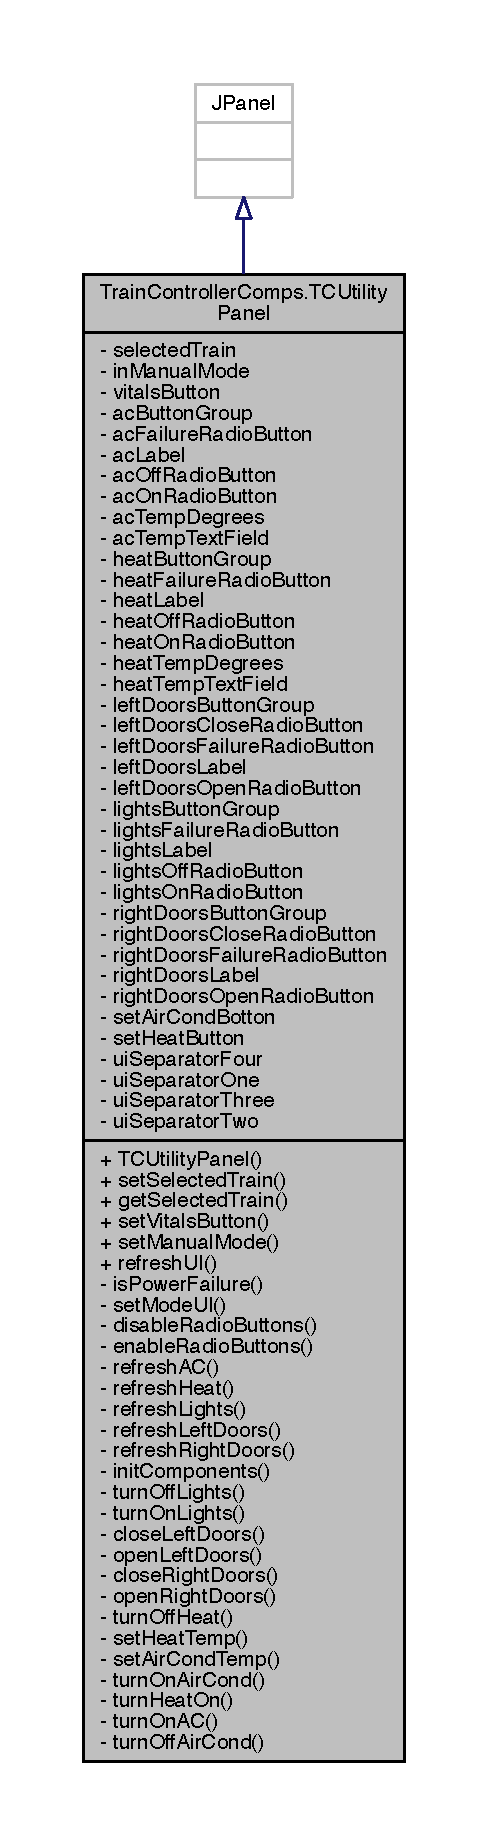
\includegraphics[height=550pt]{classTrainControllerComps_1_1TCUtilityPanel__inherit__graph}
\end{center}
\end{figure}


Collaboration diagram for Train\+Controller\+Comps.\+T\+C\+Utility\+Panel\+:
\nopagebreak
\begin{figure}[H]
\begin{center}
\leavevmode
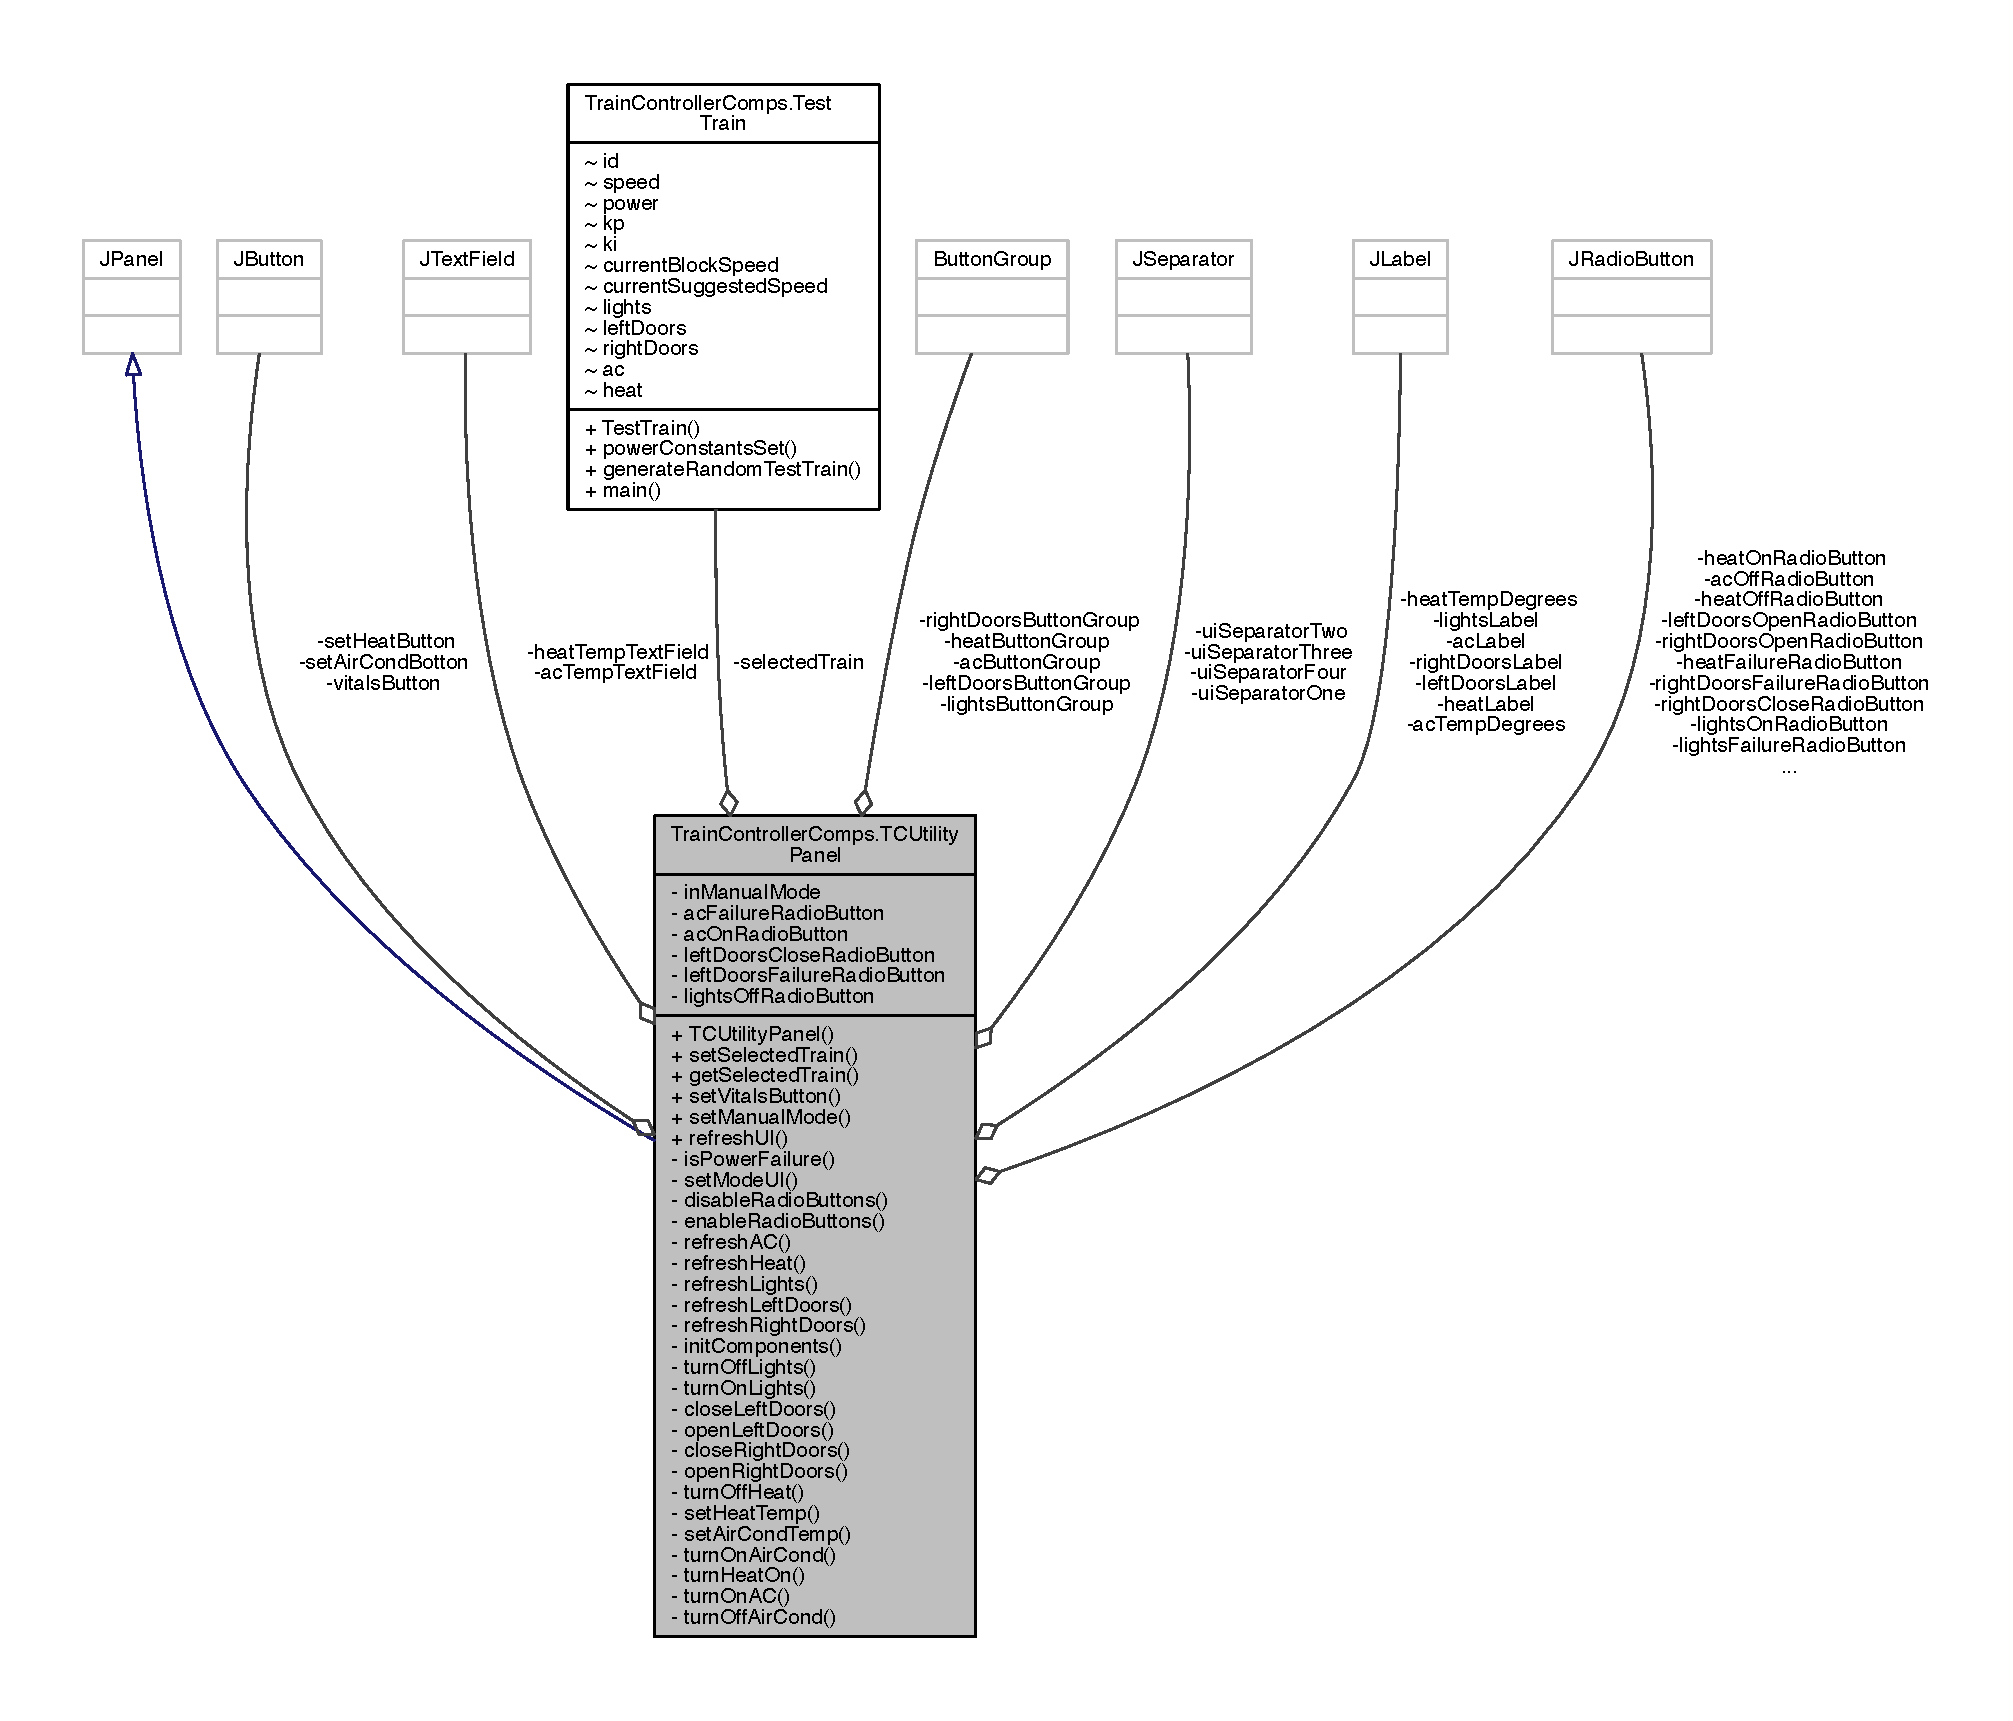
\includegraphics[width=350pt]{classTrainControllerComps_1_1TCUtilityPanel__coll__graph}
\end{center}
\end{figure}
\subsection*{Public Member Functions}
\begin{DoxyCompactItemize}
\item 
\hyperlink{classTrainControllerComps_1_1TCUtilityPanel_a0c7caafe2cb3719764e68cdb3e2b86b8}{T\+C\+Utility\+Panel} ()
\begin{DoxyCompactList}\small\item\em Constructor for creating a new T\+C\+Utiltiy\+Panel object where the initial positions of the radio button are in the \textquotesingle{}O\+FF\textquotesingle{} position, and there is no selected train. \end{DoxyCompactList}\item 
void \hyperlink{classTrainControllerComps_1_1TCUtilityPanel_aceae293b2d91b1f7d49518f1697b66d3}{set\+Selected\+Train} (\hyperlink{classTrainControllerComps_1_1TestTrain}{Test\+Train} \hyperlink{classtrain}{train})
\begin{DoxyCompactList}\small\item\em Sets the train that this Utility\+Panel should control. \end{DoxyCompactList}\item 
\hyperlink{classTrainControllerComps_1_1TestTrain}{Test\+Train} \hyperlink{classTrainControllerComps_1_1TCUtilityPanel_aa79861090681f39d2e15d9f35cc19114}{get\+Selected\+Train} ()
\begin{DoxyCompactList}\small\item\em Retrieves the train that the Utility Panel is controlling. \end{DoxyCompactList}\item 
void \hyperlink{classTrainControllerComps_1_1TCUtilityPanel_a3ec60489defa395e8f003d8f56ba4aab}{set\+Vitals\+Button} (J\+Button \hyperlink{classTrainControllerComps_1_1TCUtilityPanel_a8d0c793041cf07bd154325e0288bf7c6}{vitals\+Button})
\begin{DoxyCompactList}\small\item\em Sets the vital button. \end{DoxyCompactList}\item 
void \hyperlink{classTrainControllerComps_1_1TCUtilityPanel_a06c241551e5d282024843d8ae09bc6ba}{set\+Manual\+Mode} (boolean b)
\begin{DoxyCompactList}\small\item\em Sets if the Utility Panel should run in Manual or Automatic mode. \end{DoxyCompactList}\item 
void \hyperlink{classTrainControllerComps_1_1TCUtilityPanel_a5dd9a443969c62f13365769ef543014f}{refresh\+UI} ()
\begin{DoxyCompactList}\small\item\em Updates the UI of the radio buttons (On, Off, Fail, etc..) of the doors, lights, air conditioning, and heating unit depending on the values from the selected train. \end{DoxyCompactList}\end{DoxyCompactItemize}
\subsection*{Private Member Functions}
\begin{DoxyCompactItemize}
\item 
boolean \hyperlink{classTrainControllerComps_1_1TCUtilityPanel_acaca09d08ce4e54af81dc86ab2c768d5}{is\+Power\+Failure} ()
\begin{DoxyCompactList}\small\item\em Determines if there is a failure in one of utilities. \end{DoxyCompactList}\item 
void \hyperlink{classTrainControllerComps_1_1TCUtilityPanel_a404cb0d28b20be30802d78de9e83a831}{set\+Mode\+UI} ()
\begin{DoxyCompactList}\small\item\em Sets the UI elements that the user can interact with depending on the mode the Utility Panel is in. \end{DoxyCompactList}\item 
void \hyperlink{classTrainControllerComps_1_1TCUtilityPanel_a091dbeb6c0141d636465138a2d535613}{disable\+Radio\+Buttons} ()
\begin{DoxyCompactList}\small\item\em Disables the AC, Heat, Lights, Left/\+Right Doors radio buttons. \end{DoxyCompactList}\item 
void \hyperlink{classTrainControllerComps_1_1TCUtilityPanel_ae698554e95819802e78e7159d7319d98}{enable\+Radio\+Buttons} ()
\begin{DoxyCompactList}\small\item\em Enables the AC, Heat, Lights, Left/\+Right Doors radio buttons. \end{DoxyCompactList}\item 
void \hyperlink{classTrainControllerComps_1_1TCUtilityPanel_a0f0e32861d6be9a11dba70ce291c068d}{refresh\+AC} ()
\begin{DoxyCompactList}\small\item\em Refreshes the Air Conditioning Radio Buttons based on the status of the train. \end{DoxyCompactList}\item 
void \hyperlink{classTrainControllerComps_1_1TCUtilityPanel_a58e2492e881e7a093f62b54c2023df28}{refresh\+Heat} ()
\begin{DoxyCompactList}\small\item\em Refreshes the Heating Radio Buttons based on the status of the train. \end{DoxyCompactList}\item 
void \hyperlink{classTrainControllerComps_1_1TCUtilityPanel_a711d130d4d9c3e9c7d7513237da7bc47}{refresh\+Lights} ()
\begin{DoxyCompactList}\small\item\em Refreshes the Lights Radio Buttons based on the status of the train. \end{DoxyCompactList}\item 
void \hyperlink{classTrainControllerComps_1_1TCUtilityPanel_a698bd8e8a0c6cf25d9b4cfe38ce84504}{refresh\+Left\+Doors} ()
\begin{DoxyCompactList}\small\item\em Refreshes the Left Doors Radio Buttons based on the status of the train. \end{DoxyCompactList}\item 
void \hyperlink{classTrainControllerComps_1_1TCUtilityPanel_a8e57927dc2172cb80867b2c0582a946e}{refresh\+Right\+Doors} ()
\begin{DoxyCompactList}\small\item\em Refreshes the Right Doors Radio Buttons based on the status of the train. \end{DoxyCompactList}\item 
void \hyperlink{classTrainControllerComps_1_1TCUtilityPanel_aec618c0214d08262c146d7f941d0ce82}{init\+Components} ()
\begin{DoxyCompactList}\small\item\em This method is called from within the constructor to initialize the form. \end{DoxyCompactList}\item 
void \hyperlink{classTrainControllerComps_1_1TCUtilityPanel_a7cbaee81557b189ec438ce2bfa954c32}{turn\+Off\+Lights} (java.\+awt.\+event.\+Action\+Event evt)
\begin{DoxyCompactList}\small\item\em Tells the selected train to turn off its Lights. \end{DoxyCompactList}\item 
void \hyperlink{classTrainControllerComps_1_1TCUtilityPanel_ab82461760b088e289135115a3e038bc9}{turn\+On\+Lights} (java.\+awt.\+event.\+Action\+Event evt)
\begin{DoxyCompactList}\small\item\em Tells the selected train to turn on its Lights. \end{DoxyCompactList}\item 
void \hyperlink{classTrainControllerComps_1_1TCUtilityPanel_ab732c67358000f2bfc41eb128eab0e46}{close\+Left\+Doors} (java.\+awt.\+event.\+Action\+Event evt)
\begin{DoxyCompactList}\small\item\em Tells the selected train to close its Left Doors. \end{DoxyCompactList}\item 
void \hyperlink{classTrainControllerComps_1_1TCUtilityPanel_ab9991ca4e0a03b9e7a1b8e4fc130a4c7}{open\+Left\+Doors} (java.\+awt.\+event.\+Action\+Event evt)
\begin{DoxyCompactList}\small\item\em Tells the selected train to open its Left Doors. \end{DoxyCompactList}\item 
void \hyperlink{classTrainControllerComps_1_1TCUtilityPanel_a11c919b1746a816666bf4b9f6b03c198}{close\+Right\+Doors} (java.\+awt.\+event.\+Action\+Event evt)
\begin{DoxyCompactList}\small\item\em Tells the selected train to close its Right Doors. \end{DoxyCompactList}\item 
void \hyperlink{classTrainControllerComps_1_1TCUtilityPanel_a2c749a54d70852921749ad2821a0de91}{open\+Right\+Doors} (java.\+awt.\+event.\+Action\+Event evt)
\begin{DoxyCompactList}\small\item\em Tells the selected train to open its Right Doors. \end{DoxyCompactList}\item 
void \hyperlink{classTrainControllerComps_1_1TCUtilityPanel_a1ff45743a540a22a35ae747e4078984e}{turn\+Off\+Heat} (java.\+awt.\+event.\+Action\+Event evt)
\begin{DoxyCompactList}\small\item\em Tells the selected train to turn off the Heating unit. \end{DoxyCompactList}\item 
void \hyperlink{classTrainControllerComps_1_1TCUtilityPanel_a0123532c001a7bedfc7b4f54dbf26e5e}{set\+Heat\+Temp} (java.\+awt.\+event.\+Action\+Event evt)
\begin{DoxyCompactList}\small\item\em Tells the train to set its heating unit to the value set in the text box. \end{DoxyCompactList}\item 
void \hyperlink{classTrainControllerComps_1_1TCUtilityPanel_ac0b4656718e1a3b6d9a794b89ce5046c}{set\+Air\+Cond\+Temp} (java.\+awt.\+event.\+Action\+Event evt)
\begin{DoxyCompactList}\small\item\em Tells the train to set its air conditioning unit to the value set in the text box. \end{DoxyCompactList}\item 
void \hyperlink{classTrainControllerComps_1_1TCUtilityPanel_a542e240eb03ed81a00dc1dded248b344}{turn\+On\+Air\+Cond} (java.\+awt.\+event.\+Item\+Event evt)
\begin{DoxyCompactList}\small\item\em Currently this function is called whenever the item (Radio Button) is selected. \end{DoxyCompactList}\item 
void \hyperlink{classTrainControllerComps_1_1TCUtilityPanel_abd1bf68cdc09c79e45c5e1792961ce49}{turn\+Heat\+On} (java.\+awt.\+event.\+Item\+Event evt)
\begin{DoxyCompactList}\small\item\em Tells the train to turn on the heat, and turn off the AC if it\textquotesingle{}s on. \end{DoxyCompactList}\item 
void \hyperlink{classTrainControllerComps_1_1TCUtilityPanel_a4fbd47e0835838ba1e6bf628f7cb5f5c}{turn\+On\+AC} (java.\+awt.\+event.\+Action\+Event evt)
\item 
void \hyperlink{classTrainControllerComps_1_1TCUtilityPanel_aafe79fe4b0c04b2c00e9c7bc0e3f87c1}{turn\+Off\+Air\+Cond} (java.\+awt.\+event.\+Action\+Event evt)
\begin{DoxyCompactList}\small\item\em Tells the train to turn off the Air Conditioning unit. \end{DoxyCompactList}\end{DoxyCompactItemize}
\subsection*{Private Attributes}
\begin{DoxyCompactItemize}
\item 
\hyperlink{classTrainControllerComps_1_1TestTrain}{Test\+Train} \hyperlink{classTrainControllerComps_1_1TCUtilityPanel_a388880b551cbeb207c917c81da91baae}{selected\+Train}
\begin{DoxyCompactList}\small\item\em The train in which the UI should update from based on its values. \end{DoxyCompactList}\item 
boolean \hyperlink{classTrainControllerComps_1_1TCUtilityPanel_a40f9c46d00814e56f643a4d6dfc34364}{in\+Manual\+Mode}
\begin{DoxyCompactList}\small\item\em A boolean used to determine if the component should operate in manual or automatic mode. \end{DoxyCompactList}\item 
J\+Button \hyperlink{classTrainControllerComps_1_1TCUtilityPanel_a8d0c793041cf07bd154325e0288bf7c6}{vitals\+Button}
\begin{DoxyCompactList}\small\item\em Button used to display when a failure has occurred. \end{DoxyCompactList}\item 
javax.\+swing.\+Button\+Group \hyperlink{classTrainControllerComps_1_1TCUtilityPanel_a99c0c4bdd6c42094dcdb9c553fc92aca}{ac\+Button\+Group}
\item 
javax.\+swing.\+J\+Radio\+Button \hyperlink{classTrainControllerComps_1_1TCUtilityPanel_ab0f5fa367c6967e1e44178e88817c839}{ac\+Failure\+Radio\+Button}
\item 
javax.\+swing.\+J\+Label \hyperlink{classTrainControllerComps_1_1TCUtilityPanel_af2d327540499b3ab0cda1c5db02d1b48}{ac\+Label}
\item 
javax.\+swing.\+J\+Radio\+Button \hyperlink{classTrainControllerComps_1_1TCUtilityPanel_a7ecb1a4d7548a9626c05406474ddab6a}{ac\+Off\+Radio\+Button}
\item 
javax.\+swing.\+J\+Radio\+Button \hyperlink{classTrainControllerComps_1_1TCUtilityPanel_aab342cc326f305cf6ba11939db9cb517}{ac\+On\+Radio\+Button}
\item 
javax.\+swing.\+J\+Label \hyperlink{classTrainControllerComps_1_1TCUtilityPanel_aa3a9dd96541b8343ba7358aab1a8d3b2}{ac\+Temp\+Degrees}
\item 
javax.\+swing.\+J\+Text\+Field \hyperlink{classTrainControllerComps_1_1TCUtilityPanel_a763accf7681a5b30439a892613b85d65}{ac\+Temp\+Text\+Field}
\item 
javax.\+swing.\+Button\+Group \hyperlink{classTrainControllerComps_1_1TCUtilityPanel_a9d0cedff49b91ba6eb55ba5d2008af3f}{heat\+Button\+Group}
\item 
javax.\+swing.\+J\+Radio\+Button \hyperlink{classTrainControllerComps_1_1TCUtilityPanel_a09070da2d6a0f1dc72df800e370d7ee5}{heat\+Failure\+Radio\+Button}
\item 
javax.\+swing.\+J\+Label \hyperlink{classTrainControllerComps_1_1TCUtilityPanel_a053a72d38a0b672de8420867e95932a1}{heat\+Label}
\item 
javax.\+swing.\+J\+Radio\+Button \hyperlink{classTrainControllerComps_1_1TCUtilityPanel_a2af78f1a19af2e4327699398c9e176d1}{heat\+Off\+Radio\+Button}
\item 
javax.\+swing.\+J\+Radio\+Button \hyperlink{classTrainControllerComps_1_1TCUtilityPanel_a10f7ec26815e66e82f3591c7a52b8ec6}{heat\+On\+Radio\+Button}
\item 
javax.\+swing.\+J\+Label \hyperlink{classTrainControllerComps_1_1TCUtilityPanel_af689686006aae65099d8858c649bc5b0}{heat\+Temp\+Degrees}
\item 
javax.\+swing.\+J\+Text\+Field \hyperlink{classTrainControllerComps_1_1TCUtilityPanel_a38b738786b933b92d370dd77eff1eb85}{heat\+Temp\+Text\+Field}
\item 
javax.\+swing.\+Button\+Group \hyperlink{classTrainControllerComps_1_1TCUtilityPanel_aff1c74f0d3b06ebaba7a3a9e36f57639}{left\+Doors\+Button\+Group}
\item 
javax.\+swing.\+J\+Radio\+Button \hyperlink{classTrainControllerComps_1_1TCUtilityPanel_a430c6f0b92c2d3cbb3f47c5f5e6d0e2b}{left\+Doors\+Close\+Radio\+Button}
\item 
javax.\+swing.\+J\+Radio\+Button \hyperlink{classTrainControllerComps_1_1TCUtilityPanel_adb4176436a78a952a899922da083b3f2}{left\+Doors\+Failure\+Radio\+Button}
\item 
javax.\+swing.\+J\+Label \hyperlink{classTrainControllerComps_1_1TCUtilityPanel_adf25afb4faad696a70d9f65705cb8227}{left\+Doors\+Label}
\item 
javax.\+swing.\+J\+Radio\+Button \hyperlink{classTrainControllerComps_1_1TCUtilityPanel_aa7543914175f059490e87332386cf7bb}{left\+Doors\+Open\+Radio\+Button}
\item 
javax.\+swing.\+Button\+Group \hyperlink{classTrainControllerComps_1_1TCUtilityPanel_a5ac14cc203c357c97e40e7c485946f37}{lights\+Button\+Group}
\item 
javax.\+swing.\+J\+Radio\+Button \hyperlink{classTrainControllerComps_1_1TCUtilityPanel_a91f16bd428853a05f43ff189b237f705}{lights\+Failure\+Radio\+Button}
\item 
javax.\+swing.\+J\+Label \hyperlink{classTrainControllerComps_1_1TCUtilityPanel_af2cdc472f3b510100176138d8c5c0493}{lights\+Label}
\item 
javax.\+swing.\+J\+Radio\+Button \hyperlink{classTrainControllerComps_1_1TCUtilityPanel_a6325ef6b6e5c69f71bae4538aefa3bfe}{lights\+Off\+Radio\+Button}
\item 
javax.\+swing.\+J\+Radio\+Button \hyperlink{classTrainControllerComps_1_1TCUtilityPanel_a0a484b54e0b991752fb2fa1788e268b5}{lights\+On\+Radio\+Button}
\item 
javax.\+swing.\+Button\+Group \hyperlink{classTrainControllerComps_1_1TCUtilityPanel_ab4cb4613175b48a255aeed64c1910691}{right\+Doors\+Button\+Group}
\item 
javax.\+swing.\+J\+Radio\+Button \hyperlink{classTrainControllerComps_1_1TCUtilityPanel_a39b8a85bdbdb1d4b02e37ca2566e3a26}{right\+Doors\+Close\+Radio\+Button}
\item 
javax.\+swing.\+J\+Radio\+Button \hyperlink{classTrainControllerComps_1_1TCUtilityPanel_af612e6cbd2b7ff322efa14546b49353f}{right\+Doors\+Failure\+Radio\+Button}
\item 
javax.\+swing.\+J\+Label \hyperlink{classTrainControllerComps_1_1TCUtilityPanel_af2876ce638568941d0c05c9b4b6c87ab}{right\+Doors\+Label}
\item 
javax.\+swing.\+J\+Radio\+Button \hyperlink{classTrainControllerComps_1_1TCUtilityPanel_a768382520a1795cac4d3c783ea404ba6}{right\+Doors\+Open\+Radio\+Button}
\item 
javax.\+swing.\+J\+Button \hyperlink{classTrainControllerComps_1_1TCUtilityPanel_ae164822c9449c03c919a34c75a3865d6}{set\+Air\+Cond\+Botton}
\item 
javax.\+swing.\+J\+Button \hyperlink{classTrainControllerComps_1_1TCUtilityPanel_aaca3310ec4adf1deeb7420a0ce7003d7}{set\+Heat\+Button}
\item 
javax.\+swing.\+J\+Separator \hyperlink{classTrainControllerComps_1_1TCUtilityPanel_abd79cdd0490231c6b3bb36c364f29365}{ui\+Separator\+Four}
\item 
javax.\+swing.\+J\+Separator \hyperlink{classTrainControllerComps_1_1TCUtilityPanel_a63ffac7089464e92a93e10062b0aabad}{ui\+Separator\+One}
\item 
javax.\+swing.\+J\+Separator \hyperlink{classTrainControllerComps_1_1TCUtilityPanel_a7a48d3f3dd273c406a598cdc906b799b}{ui\+Separator\+Three}
\item 
javax.\+swing.\+J\+Separator \hyperlink{classTrainControllerComps_1_1TCUtilityPanel_aeba9dbe4e8d60298e29d5e30a2ddfdf6}{ui\+Separator\+Two}
\end{DoxyCompactItemize}


\subsection{Detailed Description}
A component of the Train Controller responsible for displaying, and transmitting information and changes to the train corresponding to the Air Conditioning unit (AC), Heating unit, Left/\+Right Doors, and Lights. 

This class collaborates with a Train Model, and the \hyperlink{classTrainControllerComps_1_1TrainController}{Train\+Controller} class, which it is a sub-\/component of.

\begin{DoxyAuthor}{Author}
Andrew Lendacky 
\end{DoxyAuthor}


\subsection{Constructor \& Destructor Documentation}
\mbox{\Hypertarget{classTrainControllerComps_1_1TCUtilityPanel_a0c7caafe2cb3719764e68cdb3e2b86b8}\label{classTrainControllerComps_1_1TCUtilityPanel_a0c7caafe2cb3719764e68cdb3e2b86b8}} 
\index{Train\+Controller\+Comps\+::\+T\+C\+Utility\+Panel@{Train\+Controller\+Comps\+::\+T\+C\+Utility\+Panel}!T\+C\+Utility\+Panel@{T\+C\+Utility\+Panel}}
\index{T\+C\+Utility\+Panel@{T\+C\+Utility\+Panel}!Train\+Controller\+Comps\+::\+T\+C\+Utility\+Panel@{Train\+Controller\+Comps\+::\+T\+C\+Utility\+Panel}}
\subsubsection{\texorpdfstring{T\+C\+Utility\+Panel()}{TCUtilityPanel()}}
{\footnotesize\ttfamily Train\+Controller\+Comps.\+T\+C\+Utility\+Panel.\+T\+C\+Utility\+Panel (\begin{DoxyParamCaption}{ }\end{DoxyParamCaption})}



Constructor for creating a new T\+C\+Utiltiy\+Panel object where the initial positions of the radio button are in the \textquotesingle{}O\+FF\textquotesingle{} position, and there is no selected train. 

By default, this constructor sets the \textquotesingle{}in\+Manual\+Mode\textquotesingle{} to false. Selected train must be set by the Train Controller before being used. 

\subsection{Member Function Documentation}
\mbox{\Hypertarget{classTrainControllerComps_1_1TCUtilityPanel_ab732c67358000f2bfc41eb128eab0e46}\label{classTrainControllerComps_1_1TCUtilityPanel_ab732c67358000f2bfc41eb128eab0e46}} 
\index{Train\+Controller\+Comps\+::\+T\+C\+Utility\+Panel@{Train\+Controller\+Comps\+::\+T\+C\+Utility\+Panel}!close\+Left\+Doors@{close\+Left\+Doors}}
\index{close\+Left\+Doors@{close\+Left\+Doors}!Train\+Controller\+Comps\+::\+T\+C\+Utility\+Panel@{Train\+Controller\+Comps\+::\+T\+C\+Utility\+Panel}}
\subsubsection{\texorpdfstring{close\+Left\+Doors()}{closeLeftDoors()}}
{\footnotesize\ttfamily void Train\+Controller\+Comps.\+T\+C\+Utility\+Panel.\+close\+Left\+Doors (\begin{DoxyParamCaption}\item[{java.\+awt.\+event.\+Action\+Event}]{evt }\end{DoxyParamCaption})\hspace{0.3cm}{\ttfamily [private]}}



Tells the selected train to close its Left Doors. 


\begin{DoxyParams}{Parameters}
{\em evt} & the sender of the action, i.\+e., the \char`\"{}\+C\+L\+O\+S\+E\char`\"{} radio button. \\
\hline
\end{DoxyParams}
\mbox{\Hypertarget{classTrainControllerComps_1_1TCUtilityPanel_a11c919b1746a816666bf4b9f6b03c198}\label{classTrainControllerComps_1_1TCUtilityPanel_a11c919b1746a816666bf4b9f6b03c198}} 
\index{Train\+Controller\+Comps\+::\+T\+C\+Utility\+Panel@{Train\+Controller\+Comps\+::\+T\+C\+Utility\+Panel}!close\+Right\+Doors@{close\+Right\+Doors}}
\index{close\+Right\+Doors@{close\+Right\+Doors}!Train\+Controller\+Comps\+::\+T\+C\+Utility\+Panel@{Train\+Controller\+Comps\+::\+T\+C\+Utility\+Panel}}
\subsubsection{\texorpdfstring{close\+Right\+Doors()}{closeRightDoors()}}
{\footnotesize\ttfamily void Train\+Controller\+Comps.\+T\+C\+Utility\+Panel.\+close\+Right\+Doors (\begin{DoxyParamCaption}\item[{java.\+awt.\+event.\+Action\+Event}]{evt }\end{DoxyParamCaption})\hspace{0.3cm}{\ttfamily [private]}}



Tells the selected train to close its Right Doors. 


\begin{DoxyParams}{Parameters}
{\em evt} & the sender of the action, i.\+e., the \char`\"{}\+C\+L\+O\+S\+E\char`\"{} radio button. \\
\hline
\end{DoxyParams}
\mbox{\Hypertarget{classTrainControllerComps_1_1TCUtilityPanel_a091dbeb6c0141d636465138a2d535613}\label{classTrainControllerComps_1_1TCUtilityPanel_a091dbeb6c0141d636465138a2d535613}} 
\index{Train\+Controller\+Comps\+::\+T\+C\+Utility\+Panel@{Train\+Controller\+Comps\+::\+T\+C\+Utility\+Panel}!disable\+Radio\+Buttons@{disable\+Radio\+Buttons}}
\index{disable\+Radio\+Buttons@{disable\+Radio\+Buttons}!Train\+Controller\+Comps\+::\+T\+C\+Utility\+Panel@{Train\+Controller\+Comps\+::\+T\+C\+Utility\+Panel}}
\subsubsection{\texorpdfstring{disable\+Radio\+Buttons()}{disableRadioButtons()}}
{\footnotesize\ttfamily void Train\+Controller\+Comps.\+T\+C\+Utility\+Panel.\+disable\+Radio\+Buttons (\begin{DoxyParamCaption}{ }\end{DoxyParamCaption})\hspace{0.3cm}{\ttfamily [private]}}



Disables the AC, Heat, Lights, Left/\+Right Doors radio buttons. 

\mbox{\Hypertarget{classTrainControllerComps_1_1TCUtilityPanel_ae698554e95819802e78e7159d7319d98}\label{classTrainControllerComps_1_1TCUtilityPanel_ae698554e95819802e78e7159d7319d98}} 
\index{Train\+Controller\+Comps\+::\+T\+C\+Utility\+Panel@{Train\+Controller\+Comps\+::\+T\+C\+Utility\+Panel}!enable\+Radio\+Buttons@{enable\+Radio\+Buttons}}
\index{enable\+Radio\+Buttons@{enable\+Radio\+Buttons}!Train\+Controller\+Comps\+::\+T\+C\+Utility\+Panel@{Train\+Controller\+Comps\+::\+T\+C\+Utility\+Panel}}
\subsubsection{\texorpdfstring{enable\+Radio\+Buttons()}{enableRadioButtons()}}
{\footnotesize\ttfamily void Train\+Controller\+Comps.\+T\+C\+Utility\+Panel.\+enable\+Radio\+Buttons (\begin{DoxyParamCaption}{ }\end{DoxyParamCaption})\hspace{0.3cm}{\ttfamily [private]}}



Enables the AC, Heat, Lights, Left/\+Right Doors radio buttons. 

\mbox{\Hypertarget{classTrainControllerComps_1_1TCUtilityPanel_aa79861090681f39d2e15d9f35cc19114}\label{classTrainControllerComps_1_1TCUtilityPanel_aa79861090681f39d2e15d9f35cc19114}} 
\index{Train\+Controller\+Comps\+::\+T\+C\+Utility\+Panel@{Train\+Controller\+Comps\+::\+T\+C\+Utility\+Panel}!get\+Selected\+Train@{get\+Selected\+Train}}
\index{get\+Selected\+Train@{get\+Selected\+Train}!Train\+Controller\+Comps\+::\+T\+C\+Utility\+Panel@{Train\+Controller\+Comps\+::\+T\+C\+Utility\+Panel}}
\subsubsection{\texorpdfstring{get\+Selected\+Train()}{getSelectedTrain()}}
{\footnotesize\ttfamily \hyperlink{classTrainControllerComps_1_1TestTrain}{Test\+Train} Train\+Controller\+Comps.\+T\+C\+Utility\+Panel.\+get\+Selected\+Train (\begin{DoxyParamCaption}{ }\end{DoxyParamCaption})}



Retrieves the train that the Utility Panel is controlling. 

\begin{DoxyReturn}{Returns}
returns the selected train. 
\end{DoxyReturn}
\mbox{\Hypertarget{classTrainControllerComps_1_1TCUtilityPanel_aec618c0214d08262c146d7f941d0ce82}\label{classTrainControllerComps_1_1TCUtilityPanel_aec618c0214d08262c146d7f941d0ce82}} 
\index{Train\+Controller\+Comps\+::\+T\+C\+Utility\+Panel@{Train\+Controller\+Comps\+::\+T\+C\+Utility\+Panel}!init\+Components@{init\+Components}}
\index{init\+Components@{init\+Components}!Train\+Controller\+Comps\+::\+T\+C\+Utility\+Panel@{Train\+Controller\+Comps\+::\+T\+C\+Utility\+Panel}}
\subsubsection{\texorpdfstring{init\+Components()}{initComponents()}}
{\footnotesize\ttfamily void Train\+Controller\+Comps.\+T\+C\+Utility\+Panel.\+init\+Components (\begin{DoxyParamCaption}{ }\end{DoxyParamCaption})\hspace{0.3cm}{\ttfamily [private]}}



This method is called from within the constructor to initialize the form. 

W\+A\+R\+N\+I\+NG\+: Do N\+OT modify this code. The content of this method is always regenerated by the Form Editor. \mbox{\Hypertarget{classTrainControllerComps_1_1TCUtilityPanel_acaca09d08ce4e54af81dc86ab2c768d5}\label{classTrainControllerComps_1_1TCUtilityPanel_acaca09d08ce4e54af81dc86ab2c768d5}} 
\index{Train\+Controller\+Comps\+::\+T\+C\+Utility\+Panel@{Train\+Controller\+Comps\+::\+T\+C\+Utility\+Panel}!is\+Power\+Failure@{is\+Power\+Failure}}
\index{is\+Power\+Failure@{is\+Power\+Failure}!Train\+Controller\+Comps\+::\+T\+C\+Utility\+Panel@{Train\+Controller\+Comps\+::\+T\+C\+Utility\+Panel}}
\subsubsection{\texorpdfstring{is\+Power\+Failure()}{isPowerFailure()}}
{\footnotesize\ttfamily boolean Train\+Controller\+Comps.\+T\+C\+Utility\+Panel.\+is\+Power\+Failure (\begin{DoxyParamCaption}{ }\end{DoxyParamCaption})\hspace{0.3cm}{\ttfamily [private]}}



Determines if there is a failure in one of utilities. 

\begin{DoxyReturn}{Returns}
returns true if at least one of the utilities are in a failure state, false otherwise. 
\end{DoxyReturn}
\mbox{\Hypertarget{classTrainControllerComps_1_1TCUtilityPanel_ab9991ca4e0a03b9e7a1b8e4fc130a4c7}\label{classTrainControllerComps_1_1TCUtilityPanel_ab9991ca4e0a03b9e7a1b8e4fc130a4c7}} 
\index{Train\+Controller\+Comps\+::\+T\+C\+Utility\+Panel@{Train\+Controller\+Comps\+::\+T\+C\+Utility\+Panel}!open\+Left\+Doors@{open\+Left\+Doors}}
\index{open\+Left\+Doors@{open\+Left\+Doors}!Train\+Controller\+Comps\+::\+T\+C\+Utility\+Panel@{Train\+Controller\+Comps\+::\+T\+C\+Utility\+Panel}}
\subsubsection{\texorpdfstring{open\+Left\+Doors()}{openLeftDoors()}}
{\footnotesize\ttfamily void Train\+Controller\+Comps.\+T\+C\+Utility\+Panel.\+open\+Left\+Doors (\begin{DoxyParamCaption}\item[{java.\+awt.\+event.\+Action\+Event}]{evt }\end{DoxyParamCaption})\hspace{0.3cm}{\ttfamily [private]}}



Tells the selected train to open its Left Doors. 


\begin{DoxyParams}{Parameters}
{\em evt} & the sender of the action, i.\+e., the \char`\"{}\+O\+P\+E\+N\char`\"{} radio button. \\
\hline
\end{DoxyParams}
\mbox{\Hypertarget{classTrainControllerComps_1_1TCUtilityPanel_a2c749a54d70852921749ad2821a0de91}\label{classTrainControllerComps_1_1TCUtilityPanel_a2c749a54d70852921749ad2821a0de91}} 
\index{Train\+Controller\+Comps\+::\+T\+C\+Utility\+Panel@{Train\+Controller\+Comps\+::\+T\+C\+Utility\+Panel}!open\+Right\+Doors@{open\+Right\+Doors}}
\index{open\+Right\+Doors@{open\+Right\+Doors}!Train\+Controller\+Comps\+::\+T\+C\+Utility\+Panel@{Train\+Controller\+Comps\+::\+T\+C\+Utility\+Panel}}
\subsubsection{\texorpdfstring{open\+Right\+Doors()}{openRightDoors()}}
{\footnotesize\ttfamily void Train\+Controller\+Comps.\+T\+C\+Utility\+Panel.\+open\+Right\+Doors (\begin{DoxyParamCaption}\item[{java.\+awt.\+event.\+Action\+Event}]{evt }\end{DoxyParamCaption})\hspace{0.3cm}{\ttfamily [private]}}



Tells the selected train to open its Right Doors. 


\begin{DoxyParams}{Parameters}
{\em evt} & the sender of the action, i.\+e., the \char`\"{}\+O\+P\+E\+N\char`\"{} radio button. \\
\hline
\end{DoxyParams}
\mbox{\Hypertarget{classTrainControllerComps_1_1TCUtilityPanel_a0f0e32861d6be9a11dba70ce291c068d}\label{classTrainControllerComps_1_1TCUtilityPanel_a0f0e32861d6be9a11dba70ce291c068d}} 
\index{Train\+Controller\+Comps\+::\+T\+C\+Utility\+Panel@{Train\+Controller\+Comps\+::\+T\+C\+Utility\+Panel}!refresh\+AC@{refresh\+AC}}
\index{refresh\+AC@{refresh\+AC}!Train\+Controller\+Comps\+::\+T\+C\+Utility\+Panel@{Train\+Controller\+Comps\+::\+T\+C\+Utility\+Panel}}
\subsubsection{\texorpdfstring{refresh\+A\+C()}{refreshAC()}}
{\footnotesize\ttfamily void Train\+Controller\+Comps.\+T\+C\+Utility\+Panel.\+refresh\+AC (\begin{DoxyParamCaption}{ }\end{DoxyParamCaption})\hspace{0.3cm}{\ttfamily [private]}}



Refreshes the Air Conditioning Radio Buttons based on the status of the train. 

This is called by the system timer every \textquotesingle{}x\textquotesingle{} seconds. function is called a lot in automatic to refresh the states of the train and have it reflected in the UI. \mbox{\Hypertarget{classTrainControllerComps_1_1TCUtilityPanel_a58e2492e881e7a093f62b54c2023df28}\label{classTrainControllerComps_1_1TCUtilityPanel_a58e2492e881e7a093f62b54c2023df28}} 
\index{Train\+Controller\+Comps\+::\+T\+C\+Utility\+Panel@{Train\+Controller\+Comps\+::\+T\+C\+Utility\+Panel}!refresh\+Heat@{refresh\+Heat}}
\index{refresh\+Heat@{refresh\+Heat}!Train\+Controller\+Comps\+::\+T\+C\+Utility\+Panel@{Train\+Controller\+Comps\+::\+T\+C\+Utility\+Panel}}
\subsubsection{\texorpdfstring{refresh\+Heat()}{refreshHeat()}}
{\footnotesize\ttfamily void Train\+Controller\+Comps.\+T\+C\+Utility\+Panel.\+refresh\+Heat (\begin{DoxyParamCaption}{ }\end{DoxyParamCaption})\hspace{0.3cm}{\ttfamily [private]}}



Refreshes the Heating Radio Buttons based on the status of the train. 

\mbox{\Hypertarget{classTrainControllerComps_1_1TCUtilityPanel_a698bd8e8a0c6cf25d9b4cfe38ce84504}\label{classTrainControllerComps_1_1TCUtilityPanel_a698bd8e8a0c6cf25d9b4cfe38ce84504}} 
\index{Train\+Controller\+Comps\+::\+T\+C\+Utility\+Panel@{Train\+Controller\+Comps\+::\+T\+C\+Utility\+Panel}!refresh\+Left\+Doors@{refresh\+Left\+Doors}}
\index{refresh\+Left\+Doors@{refresh\+Left\+Doors}!Train\+Controller\+Comps\+::\+T\+C\+Utility\+Panel@{Train\+Controller\+Comps\+::\+T\+C\+Utility\+Panel}}
\subsubsection{\texorpdfstring{refresh\+Left\+Doors()}{refreshLeftDoors()}}
{\footnotesize\ttfamily void Train\+Controller\+Comps.\+T\+C\+Utility\+Panel.\+refresh\+Left\+Doors (\begin{DoxyParamCaption}{ }\end{DoxyParamCaption})\hspace{0.3cm}{\ttfamily [private]}}



Refreshes the Left Doors Radio Buttons based on the status of the train. 

\mbox{\Hypertarget{classTrainControllerComps_1_1TCUtilityPanel_a711d130d4d9c3e9c7d7513237da7bc47}\label{classTrainControllerComps_1_1TCUtilityPanel_a711d130d4d9c3e9c7d7513237da7bc47}} 
\index{Train\+Controller\+Comps\+::\+T\+C\+Utility\+Panel@{Train\+Controller\+Comps\+::\+T\+C\+Utility\+Panel}!refresh\+Lights@{refresh\+Lights}}
\index{refresh\+Lights@{refresh\+Lights}!Train\+Controller\+Comps\+::\+T\+C\+Utility\+Panel@{Train\+Controller\+Comps\+::\+T\+C\+Utility\+Panel}}
\subsubsection{\texorpdfstring{refresh\+Lights()}{refreshLights()}}
{\footnotesize\ttfamily void Train\+Controller\+Comps.\+T\+C\+Utility\+Panel.\+refresh\+Lights (\begin{DoxyParamCaption}{ }\end{DoxyParamCaption})\hspace{0.3cm}{\ttfamily [private]}}



Refreshes the Lights Radio Buttons based on the status of the train. 

\mbox{\Hypertarget{classTrainControllerComps_1_1TCUtilityPanel_a8e57927dc2172cb80867b2c0582a946e}\label{classTrainControllerComps_1_1TCUtilityPanel_a8e57927dc2172cb80867b2c0582a946e}} 
\index{Train\+Controller\+Comps\+::\+T\+C\+Utility\+Panel@{Train\+Controller\+Comps\+::\+T\+C\+Utility\+Panel}!refresh\+Right\+Doors@{refresh\+Right\+Doors}}
\index{refresh\+Right\+Doors@{refresh\+Right\+Doors}!Train\+Controller\+Comps\+::\+T\+C\+Utility\+Panel@{Train\+Controller\+Comps\+::\+T\+C\+Utility\+Panel}}
\subsubsection{\texorpdfstring{refresh\+Right\+Doors()}{refreshRightDoors()}}
{\footnotesize\ttfamily void Train\+Controller\+Comps.\+T\+C\+Utility\+Panel.\+refresh\+Right\+Doors (\begin{DoxyParamCaption}{ }\end{DoxyParamCaption})\hspace{0.3cm}{\ttfamily [private]}}



Refreshes the Right Doors Radio Buttons based on the status of the train. 

\mbox{\Hypertarget{classTrainControllerComps_1_1TCUtilityPanel_a5dd9a443969c62f13365769ef543014f}\label{classTrainControllerComps_1_1TCUtilityPanel_a5dd9a443969c62f13365769ef543014f}} 
\index{Train\+Controller\+Comps\+::\+T\+C\+Utility\+Panel@{Train\+Controller\+Comps\+::\+T\+C\+Utility\+Panel}!refresh\+UI@{refresh\+UI}}
\index{refresh\+UI@{refresh\+UI}!Train\+Controller\+Comps\+::\+T\+C\+Utility\+Panel@{Train\+Controller\+Comps\+::\+T\+C\+Utility\+Panel}}
\subsubsection{\texorpdfstring{refresh\+U\+I()}{refreshUI()}}
{\footnotesize\ttfamily void Train\+Controller\+Comps.\+T\+C\+Utility\+Panel.\+refresh\+UI (\begin{DoxyParamCaption}{ }\end{DoxyParamCaption})}



Updates the UI of the radio buttons (On, Off, Fail, etc..) of the doors, lights, air conditioning, and heating unit depending on the values from the selected train. 

When selected a train from a T\+C\+Dispatched\+Trains\+Frame, a Null\+Pointer\+Exception is thrown.\mbox{\Hypertarget{classTrainControllerComps_1_1TCUtilityPanel_ac0b4656718e1a3b6d9a794b89ce5046c}\label{classTrainControllerComps_1_1TCUtilityPanel_ac0b4656718e1a3b6d9a794b89ce5046c}} 
\index{Train\+Controller\+Comps\+::\+T\+C\+Utility\+Panel@{Train\+Controller\+Comps\+::\+T\+C\+Utility\+Panel}!set\+Air\+Cond\+Temp@{set\+Air\+Cond\+Temp}}
\index{set\+Air\+Cond\+Temp@{set\+Air\+Cond\+Temp}!Train\+Controller\+Comps\+::\+T\+C\+Utility\+Panel@{Train\+Controller\+Comps\+::\+T\+C\+Utility\+Panel}}
\subsubsection{\texorpdfstring{set\+Air\+Cond\+Temp()}{setAirCondTemp()}}
{\footnotesize\ttfamily void Train\+Controller\+Comps.\+T\+C\+Utility\+Panel.\+set\+Air\+Cond\+Temp (\begin{DoxyParamCaption}\item[{java.\+awt.\+event.\+Action\+Event}]{evt }\end{DoxyParamCaption})\hspace{0.3cm}{\ttfamily [private]}}



Tells the train to set its air conditioning unit to the value set in the text box. 

If the set temperature of over the threshold, an error will pop up stating that the value is too high.


\begin{DoxyParams}{Parameters}
{\em evt} & the sender of the action, i.\+e., \char`\"{}\+Set\char`\"{} button. \\
\hline
\end{DoxyParams}
\mbox{\Hypertarget{classTrainControllerComps_1_1TCUtilityPanel_a0123532c001a7bedfc7b4f54dbf26e5e}\label{classTrainControllerComps_1_1TCUtilityPanel_a0123532c001a7bedfc7b4f54dbf26e5e}} 
\index{Train\+Controller\+Comps\+::\+T\+C\+Utility\+Panel@{Train\+Controller\+Comps\+::\+T\+C\+Utility\+Panel}!set\+Heat\+Temp@{set\+Heat\+Temp}}
\index{set\+Heat\+Temp@{set\+Heat\+Temp}!Train\+Controller\+Comps\+::\+T\+C\+Utility\+Panel@{Train\+Controller\+Comps\+::\+T\+C\+Utility\+Panel}}
\subsubsection{\texorpdfstring{set\+Heat\+Temp()}{setHeatTemp()}}
{\footnotesize\ttfamily void Train\+Controller\+Comps.\+T\+C\+Utility\+Panel.\+set\+Heat\+Temp (\begin{DoxyParamCaption}\item[{java.\+awt.\+event.\+Action\+Event}]{evt }\end{DoxyParamCaption})\hspace{0.3cm}{\ttfamily [private]}}



Tells the train to set its heating unit to the value set in the text box. 

If the set temperature of over the threshold, an error will pop up stating that the value is too high.


\begin{DoxyParams}{Parameters}
{\em evt} & the sender of the action, i.\+e., \char`\"{}\+Set\char`\"{} button. \\
\hline
\end{DoxyParams}
\mbox{\Hypertarget{classTrainControllerComps_1_1TCUtilityPanel_a06c241551e5d282024843d8ae09bc6ba}\label{classTrainControllerComps_1_1TCUtilityPanel_a06c241551e5d282024843d8ae09bc6ba}} 
\index{Train\+Controller\+Comps\+::\+T\+C\+Utility\+Panel@{Train\+Controller\+Comps\+::\+T\+C\+Utility\+Panel}!set\+Manual\+Mode@{set\+Manual\+Mode}}
\index{set\+Manual\+Mode@{set\+Manual\+Mode}!Train\+Controller\+Comps\+::\+T\+C\+Utility\+Panel@{Train\+Controller\+Comps\+::\+T\+C\+Utility\+Panel}}
\subsubsection{\texorpdfstring{set\+Manual\+Mode()}{setManualMode()}}
{\footnotesize\ttfamily void Train\+Controller\+Comps.\+T\+C\+Utility\+Panel.\+set\+Manual\+Mode (\begin{DoxyParamCaption}\item[{boolean}]{b }\end{DoxyParamCaption})}



Sets if the Utility Panel should run in Manual or Automatic mode. 

This value is set from the Train Controller class depending on the states of the radio buttons, \char`\"{}\+Automatic\char`\"{} and \char`\"{}\+Manual\char`\"{}.


\begin{DoxyParams}{Parameters}
{\em b} & true if in manual mode, false if in automatic mode. \\
\hline
\end{DoxyParams}
\mbox{\Hypertarget{classTrainControllerComps_1_1TCUtilityPanel_a404cb0d28b20be30802d78de9e83a831}\label{classTrainControllerComps_1_1TCUtilityPanel_a404cb0d28b20be30802d78de9e83a831}} 
\index{Train\+Controller\+Comps\+::\+T\+C\+Utility\+Panel@{Train\+Controller\+Comps\+::\+T\+C\+Utility\+Panel}!set\+Mode\+UI@{set\+Mode\+UI}}
\index{set\+Mode\+UI@{set\+Mode\+UI}!Train\+Controller\+Comps\+::\+T\+C\+Utility\+Panel@{Train\+Controller\+Comps\+::\+T\+C\+Utility\+Panel}}
\subsubsection{\texorpdfstring{set\+Mode\+U\+I()}{setModeUI()}}
{\footnotesize\ttfamily void Train\+Controller\+Comps.\+T\+C\+Utility\+Panel.\+set\+Mode\+UI (\begin{DoxyParamCaption}{ }\end{DoxyParamCaption})\hspace{0.3cm}{\ttfamily [private]}}



Sets the UI elements that the user can interact with depending on the mode the Utility Panel is in. 

\mbox{\Hypertarget{classTrainControllerComps_1_1TCUtilityPanel_aceae293b2d91b1f7d49518f1697b66d3}\label{classTrainControllerComps_1_1TCUtilityPanel_aceae293b2d91b1f7d49518f1697b66d3}} 
\index{Train\+Controller\+Comps\+::\+T\+C\+Utility\+Panel@{Train\+Controller\+Comps\+::\+T\+C\+Utility\+Panel}!set\+Selected\+Train@{set\+Selected\+Train}}
\index{set\+Selected\+Train@{set\+Selected\+Train}!Train\+Controller\+Comps\+::\+T\+C\+Utility\+Panel@{Train\+Controller\+Comps\+::\+T\+C\+Utility\+Panel}}
\subsubsection{\texorpdfstring{set\+Selected\+Train()}{setSelectedTrain()}}
{\footnotesize\ttfamily void Train\+Controller\+Comps.\+T\+C\+Utility\+Panel.\+set\+Selected\+Train (\begin{DoxyParamCaption}\item[{\hyperlink{classTrainControllerComps_1_1TestTrain}{Test\+Train}}]{train }\end{DoxyParamCaption})}



Sets the train that this Utility\+Panel should control. 

This value should be set from the Train Controller class when a new train is selected.


\begin{DoxyParams}{Parameters}
{\em train} & the train controlled by the Train Controller. \\
\hline
\end{DoxyParams}
\mbox{\Hypertarget{classTrainControllerComps_1_1TCUtilityPanel_a3ec60489defa395e8f003d8f56ba4aab}\label{classTrainControllerComps_1_1TCUtilityPanel_a3ec60489defa395e8f003d8f56ba4aab}} 
\index{Train\+Controller\+Comps\+::\+T\+C\+Utility\+Panel@{Train\+Controller\+Comps\+::\+T\+C\+Utility\+Panel}!set\+Vitals\+Button@{set\+Vitals\+Button}}
\index{set\+Vitals\+Button@{set\+Vitals\+Button}!Train\+Controller\+Comps\+::\+T\+C\+Utility\+Panel@{Train\+Controller\+Comps\+::\+T\+C\+Utility\+Panel}}
\subsubsection{\texorpdfstring{set\+Vitals\+Button()}{setVitalsButton()}}
{\footnotesize\ttfamily void Train\+Controller\+Comps.\+T\+C\+Utility\+Panel.\+set\+Vitals\+Button (\begin{DoxyParamCaption}\item[{J\+Button}]{vitals\+Button }\end{DoxyParamCaption})}



Sets the vital button. 

This method should be called from the Train Controller.


\begin{DoxyParams}{Parameters}
{\em vitals\+Button} & vital button from the Train Controller \\
\hline
\end{DoxyParams}
\mbox{\Hypertarget{classTrainControllerComps_1_1TCUtilityPanel_abd1bf68cdc09c79e45c5e1792961ce49}\label{classTrainControllerComps_1_1TCUtilityPanel_abd1bf68cdc09c79e45c5e1792961ce49}} 
\index{Train\+Controller\+Comps\+::\+T\+C\+Utility\+Panel@{Train\+Controller\+Comps\+::\+T\+C\+Utility\+Panel}!turn\+Heat\+On@{turn\+Heat\+On}}
\index{turn\+Heat\+On@{turn\+Heat\+On}!Train\+Controller\+Comps\+::\+T\+C\+Utility\+Panel@{Train\+Controller\+Comps\+::\+T\+C\+Utility\+Panel}}
\subsubsection{\texorpdfstring{turn\+Heat\+On()}{turnHeatOn()}}
{\footnotesize\ttfamily void Train\+Controller\+Comps.\+T\+C\+Utility\+Panel.\+turn\+Heat\+On (\begin{DoxyParamCaption}\item[{java.\+awt.\+event.\+Item\+Event}]{evt }\end{DoxyParamCaption})\hspace{0.3cm}{\ttfamily [private]}}



Tells the train to turn on the heat, and turn off the AC if it\textquotesingle{}s on. 

If in Manual mode, the temperature sent to the train is the value in the text box. If in Automatic mode, the temperature sent to the train is the default temperature.


\begin{DoxyParams}{Parameters}
{\em evt} & the sender of the event, i.\+e., the \textquotesingle{}ON\textquotesingle{} radio button. \\
\hline
\end{DoxyParams}
\mbox{\Hypertarget{classTrainControllerComps_1_1TCUtilityPanel_aafe79fe4b0c04b2c00e9c7bc0e3f87c1}\label{classTrainControllerComps_1_1TCUtilityPanel_aafe79fe4b0c04b2c00e9c7bc0e3f87c1}} 
\index{Train\+Controller\+Comps\+::\+T\+C\+Utility\+Panel@{Train\+Controller\+Comps\+::\+T\+C\+Utility\+Panel}!turn\+Off\+Air\+Cond@{turn\+Off\+Air\+Cond}}
\index{turn\+Off\+Air\+Cond@{turn\+Off\+Air\+Cond}!Train\+Controller\+Comps\+::\+T\+C\+Utility\+Panel@{Train\+Controller\+Comps\+::\+T\+C\+Utility\+Panel}}
\subsubsection{\texorpdfstring{turn\+Off\+Air\+Cond()}{turnOffAirCond()}}
{\footnotesize\ttfamily void Train\+Controller\+Comps.\+T\+C\+Utility\+Panel.\+turn\+Off\+Air\+Cond (\begin{DoxyParamCaption}\item[{java.\+awt.\+event.\+Action\+Event}]{evt }\end{DoxyParamCaption})\hspace{0.3cm}{\ttfamily [private]}}



Tells the train to turn off the Air Conditioning unit. 


\begin{DoxyParams}{Parameters}
{\em evt} & the sender of the event, i.\+e., the \textquotesingle{}O\+FF\textquotesingle{} radio button. \\
\hline
\end{DoxyParams}
\mbox{\Hypertarget{classTrainControllerComps_1_1TCUtilityPanel_a1ff45743a540a22a35ae747e4078984e}\label{classTrainControllerComps_1_1TCUtilityPanel_a1ff45743a540a22a35ae747e4078984e}} 
\index{Train\+Controller\+Comps\+::\+T\+C\+Utility\+Panel@{Train\+Controller\+Comps\+::\+T\+C\+Utility\+Panel}!turn\+Off\+Heat@{turn\+Off\+Heat}}
\index{turn\+Off\+Heat@{turn\+Off\+Heat}!Train\+Controller\+Comps\+::\+T\+C\+Utility\+Panel@{Train\+Controller\+Comps\+::\+T\+C\+Utility\+Panel}}
\subsubsection{\texorpdfstring{turn\+Off\+Heat()}{turnOffHeat()}}
{\footnotesize\ttfamily void Train\+Controller\+Comps.\+T\+C\+Utility\+Panel.\+turn\+Off\+Heat (\begin{DoxyParamCaption}\item[{java.\+awt.\+event.\+Action\+Event}]{evt }\end{DoxyParamCaption})\hspace{0.3cm}{\ttfamily [private]}}



Tells the selected train to turn off the Heating unit. 


\begin{DoxyParams}{Parameters}
{\em evt} & the sender of the action, i.\+e., the \char`\"{}\+O\+F\+F\char`\"{} radio button. \\
\hline
\end{DoxyParams}
\mbox{\Hypertarget{classTrainControllerComps_1_1TCUtilityPanel_a7cbaee81557b189ec438ce2bfa954c32}\label{classTrainControllerComps_1_1TCUtilityPanel_a7cbaee81557b189ec438ce2bfa954c32}} 
\index{Train\+Controller\+Comps\+::\+T\+C\+Utility\+Panel@{Train\+Controller\+Comps\+::\+T\+C\+Utility\+Panel}!turn\+Off\+Lights@{turn\+Off\+Lights}}
\index{turn\+Off\+Lights@{turn\+Off\+Lights}!Train\+Controller\+Comps\+::\+T\+C\+Utility\+Panel@{Train\+Controller\+Comps\+::\+T\+C\+Utility\+Panel}}
\subsubsection{\texorpdfstring{turn\+Off\+Lights()}{turnOffLights()}}
{\footnotesize\ttfamily void Train\+Controller\+Comps.\+T\+C\+Utility\+Panel.\+turn\+Off\+Lights (\begin{DoxyParamCaption}\item[{java.\+awt.\+event.\+Action\+Event}]{evt }\end{DoxyParamCaption})\hspace{0.3cm}{\ttfamily [private]}}



Tells the selected train to turn off its Lights. 

This occurs when the \char`\"{}\+O\+F\+F\char`\"{} radio button is clicked.


\begin{DoxyParams}{Parameters}
{\em evt} & the sender of the action, i.\+e., the \char`\"{}\+O\+F\+F\char`\"{} radio button. \\
\hline
\end{DoxyParams}
\mbox{\Hypertarget{classTrainControllerComps_1_1TCUtilityPanel_a4fbd47e0835838ba1e6bf628f7cb5f5c}\label{classTrainControllerComps_1_1TCUtilityPanel_a4fbd47e0835838ba1e6bf628f7cb5f5c}} 
\index{Train\+Controller\+Comps\+::\+T\+C\+Utility\+Panel@{Train\+Controller\+Comps\+::\+T\+C\+Utility\+Panel}!turn\+On\+AC@{turn\+On\+AC}}
\index{turn\+On\+AC@{turn\+On\+AC}!Train\+Controller\+Comps\+::\+T\+C\+Utility\+Panel@{Train\+Controller\+Comps\+::\+T\+C\+Utility\+Panel}}
\subsubsection{\texorpdfstring{turn\+On\+A\+C()}{turnOnAC()}}
{\footnotesize\ttfamily void Train\+Controller\+Comps.\+T\+C\+Utility\+Panel.\+turn\+On\+AC (\begin{DoxyParamCaption}\item[{java.\+awt.\+event.\+Action\+Event}]{evt }\end{DoxyParamCaption})\hspace{0.3cm}{\ttfamily [private]}}

\mbox{\Hypertarget{classTrainControllerComps_1_1TCUtilityPanel_a542e240eb03ed81a00dc1dded248b344}\label{classTrainControllerComps_1_1TCUtilityPanel_a542e240eb03ed81a00dc1dded248b344}} 
\index{Train\+Controller\+Comps\+::\+T\+C\+Utility\+Panel@{Train\+Controller\+Comps\+::\+T\+C\+Utility\+Panel}!turn\+On\+Air\+Cond@{turn\+On\+Air\+Cond}}
\index{turn\+On\+Air\+Cond@{turn\+On\+Air\+Cond}!Train\+Controller\+Comps\+::\+T\+C\+Utility\+Panel@{Train\+Controller\+Comps\+::\+T\+C\+Utility\+Panel}}
\subsubsection{\texorpdfstring{turn\+On\+Air\+Cond()}{turnOnAirCond()}}
{\footnotesize\ttfamily void Train\+Controller\+Comps.\+T\+C\+Utility\+Panel.\+turn\+On\+Air\+Cond (\begin{DoxyParamCaption}\item[{java.\+awt.\+event.\+Item\+Event}]{evt }\end{DoxyParamCaption})\hspace{0.3cm}{\ttfamily [private]}}



Currently this function is called whenever the item (Radio Button) is selected. 

This should be the code that sends the information to the train regarding the states of on the train.

Clicking the \textquotesingle{}Set\textquotesingle{} button causes the G\+UI to change to \textquotesingle{}On\textquotesingle{}, and

F\+I\+X\+E\+D!


\begin{DoxyParams}{Parameters}
{\em evt} & Clicking the \textquotesingle{}On\textquotesingle{} button will set the temperature to the default temp instead of resending the temp that was previously in the text field.\\
\hline
\end{DoxyParams}
Replicate by Tells the train to turn on the Air Conditioning unit, and to turn off the heat if it\textquotesingle{}s on. If in Manual mode, the temperature sent to the train is the value in the text box. If in Automatic mode, the temperature sent to the train is the default temperature.


\begin{DoxyParams}{Parameters}
{\em evt} & the sender of the event, i.\+e, the \textquotesingle{}ON\textquotesingle{} radio button. \\
\hline
\end{DoxyParams}
\mbox{\Hypertarget{classTrainControllerComps_1_1TCUtilityPanel_ab82461760b088e289135115a3e038bc9}\label{classTrainControllerComps_1_1TCUtilityPanel_ab82461760b088e289135115a3e038bc9}} 
\index{Train\+Controller\+Comps\+::\+T\+C\+Utility\+Panel@{Train\+Controller\+Comps\+::\+T\+C\+Utility\+Panel}!turn\+On\+Lights@{turn\+On\+Lights}}
\index{turn\+On\+Lights@{turn\+On\+Lights}!Train\+Controller\+Comps\+::\+T\+C\+Utility\+Panel@{Train\+Controller\+Comps\+::\+T\+C\+Utility\+Panel}}
\subsubsection{\texorpdfstring{turn\+On\+Lights()}{turnOnLights()}}
{\footnotesize\ttfamily void Train\+Controller\+Comps.\+T\+C\+Utility\+Panel.\+turn\+On\+Lights (\begin{DoxyParamCaption}\item[{java.\+awt.\+event.\+Action\+Event}]{evt }\end{DoxyParamCaption})\hspace{0.3cm}{\ttfamily [private]}}



Tells the selected train to turn on its Lights. 


\begin{DoxyParams}{Parameters}
{\em evt} & the sender of the action, i.\+e., the \char`\"{}\+O\+N\char`\"{} radio button. \\
\hline
\end{DoxyParams}


\subsection{Member Data Documentation}
\mbox{\Hypertarget{classTrainControllerComps_1_1TCUtilityPanel_a99c0c4bdd6c42094dcdb9c553fc92aca}\label{classTrainControllerComps_1_1TCUtilityPanel_a99c0c4bdd6c42094dcdb9c553fc92aca}} 
\index{Train\+Controller\+Comps\+::\+T\+C\+Utility\+Panel@{Train\+Controller\+Comps\+::\+T\+C\+Utility\+Panel}!ac\+Button\+Group@{ac\+Button\+Group}}
\index{ac\+Button\+Group@{ac\+Button\+Group}!Train\+Controller\+Comps\+::\+T\+C\+Utility\+Panel@{Train\+Controller\+Comps\+::\+T\+C\+Utility\+Panel}}
\subsubsection{\texorpdfstring{ac\+Button\+Group}{acButtonGroup}}
{\footnotesize\ttfamily javax.\+swing.\+Button\+Group Train\+Controller\+Comps.\+T\+C\+Utility\+Panel.\+ac\+Button\+Group\hspace{0.3cm}{\ttfamily [private]}}

\mbox{\Hypertarget{classTrainControllerComps_1_1TCUtilityPanel_ab0f5fa367c6967e1e44178e88817c839}\label{classTrainControllerComps_1_1TCUtilityPanel_ab0f5fa367c6967e1e44178e88817c839}} 
\index{Train\+Controller\+Comps\+::\+T\+C\+Utility\+Panel@{Train\+Controller\+Comps\+::\+T\+C\+Utility\+Panel}!ac\+Failure\+Radio\+Button@{ac\+Failure\+Radio\+Button}}
\index{ac\+Failure\+Radio\+Button@{ac\+Failure\+Radio\+Button}!Train\+Controller\+Comps\+::\+T\+C\+Utility\+Panel@{Train\+Controller\+Comps\+::\+T\+C\+Utility\+Panel}}
\subsubsection{\texorpdfstring{ac\+Failure\+Radio\+Button}{acFailureRadioButton}}
{\footnotesize\ttfamily javax.\+swing.\+J\+Radio\+Button Train\+Controller\+Comps.\+T\+C\+Utility\+Panel.\+ac\+Failure\+Radio\+Button\hspace{0.3cm}{\ttfamily [private]}}

\mbox{\Hypertarget{classTrainControllerComps_1_1TCUtilityPanel_af2d327540499b3ab0cda1c5db02d1b48}\label{classTrainControllerComps_1_1TCUtilityPanel_af2d327540499b3ab0cda1c5db02d1b48}} 
\index{Train\+Controller\+Comps\+::\+T\+C\+Utility\+Panel@{Train\+Controller\+Comps\+::\+T\+C\+Utility\+Panel}!ac\+Label@{ac\+Label}}
\index{ac\+Label@{ac\+Label}!Train\+Controller\+Comps\+::\+T\+C\+Utility\+Panel@{Train\+Controller\+Comps\+::\+T\+C\+Utility\+Panel}}
\subsubsection{\texorpdfstring{ac\+Label}{acLabel}}
{\footnotesize\ttfamily javax.\+swing.\+J\+Label Train\+Controller\+Comps.\+T\+C\+Utility\+Panel.\+ac\+Label\hspace{0.3cm}{\ttfamily [private]}}

\mbox{\Hypertarget{classTrainControllerComps_1_1TCUtilityPanel_a7ecb1a4d7548a9626c05406474ddab6a}\label{classTrainControllerComps_1_1TCUtilityPanel_a7ecb1a4d7548a9626c05406474ddab6a}} 
\index{Train\+Controller\+Comps\+::\+T\+C\+Utility\+Panel@{Train\+Controller\+Comps\+::\+T\+C\+Utility\+Panel}!ac\+Off\+Radio\+Button@{ac\+Off\+Radio\+Button}}
\index{ac\+Off\+Radio\+Button@{ac\+Off\+Radio\+Button}!Train\+Controller\+Comps\+::\+T\+C\+Utility\+Panel@{Train\+Controller\+Comps\+::\+T\+C\+Utility\+Panel}}
\subsubsection{\texorpdfstring{ac\+Off\+Radio\+Button}{acOffRadioButton}}
{\footnotesize\ttfamily javax.\+swing.\+J\+Radio\+Button Train\+Controller\+Comps.\+T\+C\+Utility\+Panel.\+ac\+Off\+Radio\+Button\hspace{0.3cm}{\ttfamily [private]}}

\mbox{\Hypertarget{classTrainControllerComps_1_1TCUtilityPanel_aab342cc326f305cf6ba11939db9cb517}\label{classTrainControllerComps_1_1TCUtilityPanel_aab342cc326f305cf6ba11939db9cb517}} 
\index{Train\+Controller\+Comps\+::\+T\+C\+Utility\+Panel@{Train\+Controller\+Comps\+::\+T\+C\+Utility\+Panel}!ac\+On\+Radio\+Button@{ac\+On\+Radio\+Button}}
\index{ac\+On\+Radio\+Button@{ac\+On\+Radio\+Button}!Train\+Controller\+Comps\+::\+T\+C\+Utility\+Panel@{Train\+Controller\+Comps\+::\+T\+C\+Utility\+Panel}}
\subsubsection{\texorpdfstring{ac\+On\+Radio\+Button}{acOnRadioButton}}
{\footnotesize\ttfamily javax.\+swing.\+J\+Radio\+Button Train\+Controller\+Comps.\+T\+C\+Utility\+Panel.\+ac\+On\+Radio\+Button\hspace{0.3cm}{\ttfamily [private]}}

\mbox{\Hypertarget{classTrainControllerComps_1_1TCUtilityPanel_aa3a9dd96541b8343ba7358aab1a8d3b2}\label{classTrainControllerComps_1_1TCUtilityPanel_aa3a9dd96541b8343ba7358aab1a8d3b2}} 
\index{Train\+Controller\+Comps\+::\+T\+C\+Utility\+Panel@{Train\+Controller\+Comps\+::\+T\+C\+Utility\+Panel}!ac\+Temp\+Degrees@{ac\+Temp\+Degrees}}
\index{ac\+Temp\+Degrees@{ac\+Temp\+Degrees}!Train\+Controller\+Comps\+::\+T\+C\+Utility\+Panel@{Train\+Controller\+Comps\+::\+T\+C\+Utility\+Panel}}
\subsubsection{\texorpdfstring{ac\+Temp\+Degrees}{acTempDegrees}}
{\footnotesize\ttfamily javax.\+swing.\+J\+Label Train\+Controller\+Comps.\+T\+C\+Utility\+Panel.\+ac\+Temp\+Degrees\hspace{0.3cm}{\ttfamily [private]}}

\mbox{\Hypertarget{classTrainControllerComps_1_1TCUtilityPanel_a763accf7681a5b30439a892613b85d65}\label{classTrainControllerComps_1_1TCUtilityPanel_a763accf7681a5b30439a892613b85d65}} 
\index{Train\+Controller\+Comps\+::\+T\+C\+Utility\+Panel@{Train\+Controller\+Comps\+::\+T\+C\+Utility\+Panel}!ac\+Temp\+Text\+Field@{ac\+Temp\+Text\+Field}}
\index{ac\+Temp\+Text\+Field@{ac\+Temp\+Text\+Field}!Train\+Controller\+Comps\+::\+T\+C\+Utility\+Panel@{Train\+Controller\+Comps\+::\+T\+C\+Utility\+Panel}}
\subsubsection{\texorpdfstring{ac\+Temp\+Text\+Field}{acTempTextField}}
{\footnotesize\ttfamily javax.\+swing.\+J\+Text\+Field Train\+Controller\+Comps.\+T\+C\+Utility\+Panel.\+ac\+Temp\+Text\+Field\hspace{0.3cm}{\ttfamily [private]}}

\mbox{\Hypertarget{classTrainControllerComps_1_1TCUtilityPanel_a9d0cedff49b91ba6eb55ba5d2008af3f}\label{classTrainControllerComps_1_1TCUtilityPanel_a9d0cedff49b91ba6eb55ba5d2008af3f}} 
\index{Train\+Controller\+Comps\+::\+T\+C\+Utility\+Panel@{Train\+Controller\+Comps\+::\+T\+C\+Utility\+Panel}!heat\+Button\+Group@{heat\+Button\+Group}}
\index{heat\+Button\+Group@{heat\+Button\+Group}!Train\+Controller\+Comps\+::\+T\+C\+Utility\+Panel@{Train\+Controller\+Comps\+::\+T\+C\+Utility\+Panel}}
\subsubsection{\texorpdfstring{heat\+Button\+Group}{heatButtonGroup}}
{\footnotesize\ttfamily javax.\+swing.\+Button\+Group Train\+Controller\+Comps.\+T\+C\+Utility\+Panel.\+heat\+Button\+Group\hspace{0.3cm}{\ttfamily [private]}}

\mbox{\Hypertarget{classTrainControllerComps_1_1TCUtilityPanel_a09070da2d6a0f1dc72df800e370d7ee5}\label{classTrainControllerComps_1_1TCUtilityPanel_a09070da2d6a0f1dc72df800e370d7ee5}} 
\index{Train\+Controller\+Comps\+::\+T\+C\+Utility\+Panel@{Train\+Controller\+Comps\+::\+T\+C\+Utility\+Panel}!heat\+Failure\+Radio\+Button@{heat\+Failure\+Radio\+Button}}
\index{heat\+Failure\+Radio\+Button@{heat\+Failure\+Radio\+Button}!Train\+Controller\+Comps\+::\+T\+C\+Utility\+Panel@{Train\+Controller\+Comps\+::\+T\+C\+Utility\+Panel}}
\subsubsection{\texorpdfstring{heat\+Failure\+Radio\+Button}{heatFailureRadioButton}}
{\footnotesize\ttfamily javax.\+swing.\+J\+Radio\+Button Train\+Controller\+Comps.\+T\+C\+Utility\+Panel.\+heat\+Failure\+Radio\+Button\hspace{0.3cm}{\ttfamily [private]}}

\mbox{\Hypertarget{classTrainControllerComps_1_1TCUtilityPanel_a053a72d38a0b672de8420867e95932a1}\label{classTrainControllerComps_1_1TCUtilityPanel_a053a72d38a0b672de8420867e95932a1}} 
\index{Train\+Controller\+Comps\+::\+T\+C\+Utility\+Panel@{Train\+Controller\+Comps\+::\+T\+C\+Utility\+Panel}!heat\+Label@{heat\+Label}}
\index{heat\+Label@{heat\+Label}!Train\+Controller\+Comps\+::\+T\+C\+Utility\+Panel@{Train\+Controller\+Comps\+::\+T\+C\+Utility\+Panel}}
\subsubsection{\texorpdfstring{heat\+Label}{heatLabel}}
{\footnotesize\ttfamily javax.\+swing.\+J\+Label Train\+Controller\+Comps.\+T\+C\+Utility\+Panel.\+heat\+Label\hspace{0.3cm}{\ttfamily [private]}}

\mbox{\Hypertarget{classTrainControllerComps_1_1TCUtilityPanel_a2af78f1a19af2e4327699398c9e176d1}\label{classTrainControllerComps_1_1TCUtilityPanel_a2af78f1a19af2e4327699398c9e176d1}} 
\index{Train\+Controller\+Comps\+::\+T\+C\+Utility\+Panel@{Train\+Controller\+Comps\+::\+T\+C\+Utility\+Panel}!heat\+Off\+Radio\+Button@{heat\+Off\+Radio\+Button}}
\index{heat\+Off\+Radio\+Button@{heat\+Off\+Radio\+Button}!Train\+Controller\+Comps\+::\+T\+C\+Utility\+Panel@{Train\+Controller\+Comps\+::\+T\+C\+Utility\+Panel}}
\subsubsection{\texorpdfstring{heat\+Off\+Radio\+Button}{heatOffRadioButton}}
{\footnotesize\ttfamily javax.\+swing.\+J\+Radio\+Button Train\+Controller\+Comps.\+T\+C\+Utility\+Panel.\+heat\+Off\+Radio\+Button\hspace{0.3cm}{\ttfamily [private]}}

\mbox{\Hypertarget{classTrainControllerComps_1_1TCUtilityPanel_a10f7ec26815e66e82f3591c7a52b8ec6}\label{classTrainControllerComps_1_1TCUtilityPanel_a10f7ec26815e66e82f3591c7a52b8ec6}} 
\index{Train\+Controller\+Comps\+::\+T\+C\+Utility\+Panel@{Train\+Controller\+Comps\+::\+T\+C\+Utility\+Panel}!heat\+On\+Radio\+Button@{heat\+On\+Radio\+Button}}
\index{heat\+On\+Radio\+Button@{heat\+On\+Radio\+Button}!Train\+Controller\+Comps\+::\+T\+C\+Utility\+Panel@{Train\+Controller\+Comps\+::\+T\+C\+Utility\+Panel}}
\subsubsection{\texorpdfstring{heat\+On\+Radio\+Button}{heatOnRadioButton}}
{\footnotesize\ttfamily javax.\+swing.\+J\+Radio\+Button Train\+Controller\+Comps.\+T\+C\+Utility\+Panel.\+heat\+On\+Radio\+Button\hspace{0.3cm}{\ttfamily [private]}}

\mbox{\Hypertarget{classTrainControllerComps_1_1TCUtilityPanel_af689686006aae65099d8858c649bc5b0}\label{classTrainControllerComps_1_1TCUtilityPanel_af689686006aae65099d8858c649bc5b0}} 
\index{Train\+Controller\+Comps\+::\+T\+C\+Utility\+Panel@{Train\+Controller\+Comps\+::\+T\+C\+Utility\+Panel}!heat\+Temp\+Degrees@{heat\+Temp\+Degrees}}
\index{heat\+Temp\+Degrees@{heat\+Temp\+Degrees}!Train\+Controller\+Comps\+::\+T\+C\+Utility\+Panel@{Train\+Controller\+Comps\+::\+T\+C\+Utility\+Panel}}
\subsubsection{\texorpdfstring{heat\+Temp\+Degrees}{heatTempDegrees}}
{\footnotesize\ttfamily javax.\+swing.\+J\+Label Train\+Controller\+Comps.\+T\+C\+Utility\+Panel.\+heat\+Temp\+Degrees\hspace{0.3cm}{\ttfamily [private]}}

\mbox{\Hypertarget{classTrainControllerComps_1_1TCUtilityPanel_a38b738786b933b92d370dd77eff1eb85}\label{classTrainControllerComps_1_1TCUtilityPanel_a38b738786b933b92d370dd77eff1eb85}} 
\index{Train\+Controller\+Comps\+::\+T\+C\+Utility\+Panel@{Train\+Controller\+Comps\+::\+T\+C\+Utility\+Panel}!heat\+Temp\+Text\+Field@{heat\+Temp\+Text\+Field}}
\index{heat\+Temp\+Text\+Field@{heat\+Temp\+Text\+Field}!Train\+Controller\+Comps\+::\+T\+C\+Utility\+Panel@{Train\+Controller\+Comps\+::\+T\+C\+Utility\+Panel}}
\subsubsection{\texorpdfstring{heat\+Temp\+Text\+Field}{heatTempTextField}}
{\footnotesize\ttfamily javax.\+swing.\+J\+Text\+Field Train\+Controller\+Comps.\+T\+C\+Utility\+Panel.\+heat\+Temp\+Text\+Field\hspace{0.3cm}{\ttfamily [private]}}

\mbox{\Hypertarget{classTrainControllerComps_1_1TCUtilityPanel_a40f9c46d00814e56f643a4d6dfc34364}\label{classTrainControllerComps_1_1TCUtilityPanel_a40f9c46d00814e56f643a4d6dfc34364}} 
\index{Train\+Controller\+Comps\+::\+T\+C\+Utility\+Panel@{Train\+Controller\+Comps\+::\+T\+C\+Utility\+Panel}!in\+Manual\+Mode@{in\+Manual\+Mode}}
\index{in\+Manual\+Mode@{in\+Manual\+Mode}!Train\+Controller\+Comps\+::\+T\+C\+Utility\+Panel@{Train\+Controller\+Comps\+::\+T\+C\+Utility\+Panel}}
\subsubsection{\texorpdfstring{in\+Manual\+Mode}{inManualMode}}
{\footnotesize\ttfamily boolean Train\+Controller\+Comps.\+T\+C\+Utility\+Panel.\+in\+Manual\+Mode\hspace{0.3cm}{\ttfamily [private]}}



A boolean used to determine if the component should operate in manual or automatic mode. 

This value gets set from the \hyperlink{classTrainControllerComps_1_1TrainController}{Train\+Controller} class. \mbox{\Hypertarget{classTrainControllerComps_1_1TCUtilityPanel_aff1c74f0d3b06ebaba7a3a9e36f57639}\label{classTrainControllerComps_1_1TCUtilityPanel_aff1c74f0d3b06ebaba7a3a9e36f57639}} 
\index{Train\+Controller\+Comps\+::\+T\+C\+Utility\+Panel@{Train\+Controller\+Comps\+::\+T\+C\+Utility\+Panel}!left\+Doors\+Button\+Group@{left\+Doors\+Button\+Group}}
\index{left\+Doors\+Button\+Group@{left\+Doors\+Button\+Group}!Train\+Controller\+Comps\+::\+T\+C\+Utility\+Panel@{Train\+Controller\+Comps\+::\+T\+C\+Utility\+Panel}}
\subsubsection{\texorpdfstring{left\+Doors\+Button\+Group}{leftDoorsButtonGroup}}
{\footnotesize\ttfamily javax.\+swing.\+Button\+Group Train\+Controller\+Comps.\+T\+C\+Utility\+Panel.\+left\+Doors\+Button\+Group\hspace{0.3cm}{\ttfamily [private]}}

\mbox{\Hypertarget{classTrainControllerComps_1_1TCUtilityPanel_a430c6f0b92c2d3cbb3f47c5f5e6d0e2b}\label{classTrainControllerComps_1_1TCUtilityPanel_a430c6f0b92c2d3cbb3f47c5f5e6d0e2b}} 
\index{Train\+Controller\+Comps\+::\+T\+C\+Utility\+Panel@{Train\+Controller\+Comps\+::\+T\+C\+Utility\+Panel}!left\+Doors\+Close\+Radio\+Button@{left\+Doors\+Close\+Radio\+Button}}
\index{left\+Doors\+Close\+Radio\+Button@{left\+Doors\+Close\+Radio\+Button}!Train\+Controller\+Comps\+::\+T\+C\+Utility\+Panel@{Train\+Controller\+Comps\+::\+T\+C\+Utility\+Panel}}
\subsubsection{\texorpdfstring{left\+Doors\+Close\+Radio\+Button}{leftDoorsCloseRadioButton}}
{\footnotesize\ttfamily javax.\+swing.\+J\+Radio\+Button Train\+Controller\+Comps.\+T\+C\+Utility\+Panel.\+left\+Doors\+Close\+Radio\+Button\hspace{0.3cm}{\ttfamily [private]}}

\mbox{\Hypertarget{classTrainControllerComps_1_1TCUtilityPanel_adb4176436a78a952a899922da083b3f2}\label{classTrainControllerComps_1_1TCUtilityPanel_adb4176436a78a952a899922da083b3f2}} 
\index{Train\+Controller\+Comps\+::\+T\+C\+Utility\+Panel@{Train\+Controller\+Comps\+::\+T\+C\+Utility\+Panel}!left\+Doors\+Failure\+Radio\+Button@{left\+Doors\+Failure\+Radio\+Button}}
\index{left\+Doors\+Failure\+Radio\+Button@{left\+Doors\+Failure\+Radio\+Button}!Train\+Controller\+Comps\+::\+T\+C\+Utility\+Panel@{Train\+Controller\+Comps\+::\+T\+C\+Utility\+Panel}}
\subsubsection{\texorpdfstring{left\+Doors\+Failure\+Radio\+Button}{leftDoorsFailureRadioButton}}
{\footnotesize\ttfamily javax.\+swing.\+J\+Radio\+Button Train\+Controller\+Comps.\+T\+C\+Utility\+Panel.\+left\+Doors\+Failure\+Radio\+Button\hspace{0.3cm}{\ttfamily [private]}}

\mbox{\Hypertarget{classTrainControllerComps_1_1TCUtilityPanel_adf25afb4faad696a70d9f65705cb8227}\label{classTrainControllerComps_1_1TCUtilityPanel_adf25afb4faad696a70d9f65705cb8227}} 
\index{Train\+Controller\+Comps\+::\+T\+C\+Utility\+Panel@{Train\+Controller\+Comps\+::\+T\+C\+Utility\+Panel}!left\+Doors\+Label@{left\+Doors\+Label}}
\index{left\+Doors\+Label@{left\+Doors\+Label}!Train\+Controller\+Comps\+::\+T\+C\+Utility\+Panel@{Train\+Controller\+Comps\+::\+T\+C\+Utility\+Panel}}
\subsubsection{\texorpdfstring{left\+Doors\+Label}{leftDoorsLabel}}
{\footnotesize\ttfamily javax.\+swing.\+J\+Label Train\+Controller\+Comps.\+T\+C\+Utility\+Panel.\+left\+Doors\+Label\hspace{0.3cm}{\ttfamily [private]}}

\mbox{\Hypertarget{classTrainControllerComps_1_1TCUtilityPanel_aa7543914175f059490e87332386cf7bb}\label{classTrainControllerComps_1_1TCUtilityPanel_aa7543914175f059490e87332386cf7bb}} 
\index{Train\+Controller\+Comps\+::\+T\+C\+Utility\+Panel@{Train\+Controller\+Comps\+::\+T\+C\+Utility\+Panel}!left\+Doors\+Open\+Radio\+Button@{left\+Doors\+Open\+Radio\+Button}}
\index{left\+Doors\+Open\+Radio\+Button@{left\+Doors\+Open\+Radio\+Button}!Train\+Controller\+Comps\+::\+T\+C\+Utility\+Panel@{Train\+Controller\+Comps\+::\+T\+C\+Utility\+Panel}}
\subsubsection{\texorpdfstring{left\+Doors\+Open\+Radio\+Button}{leftDoorsOpenRadioButton}}
{\footnotesize\ttfamily javax.\+swing.\+J\+Radio\+Button Train\+Controller\+Comps.\+T\+C\+Utility\+Panel.\+left\+Doors\+Open\+Radio\+Button\hspace{0.3cm}{\ttfamily [private]}}

\mbox{\Hypertarget{classTrainControllerComps_1_1TCUtilityPanel_a5ac14cc203c357c97e40e7c485946f37}\label{classTrainControllerComps_1_1TCUtilityPanel_a5ac14cc203c357c97e40e7c485946f37}} 
\index{Train\+Controller\+Comps\+::\+T\+C\+Utility\+Panel@{Train\+Controller\+Comps\+::\+T\+C\+Utility\+Panel}!lights\+Button\+Group@{lights\+Button\+Group}}
\index{lights\+Button\+Group@{lights\+Button\+Group}!Train\+Controller\+Comps\+::\+T\+C\+Utility\+Panel@{Train\+Controller\+Comps\+::\+T\+C\+Utility\+Panel}}
\subsubsection{\texorpdfstring{lights\+Button\+Group}{lightsButtonGroup}}
{\footnotesize\ttfamily javax.\+swing.\+Button\+Group Train\+Controller\+Comps.\+T\+C\+Utility\+Panel.\+lights\+Button\+Group\hspace{0.3cm}{\ttfamily [private]}}

\mbox{\Hypertarget{classTrainControllerComps_1_1TCUtilityPanel_a91f16bd428853a05f43ff189b237f705}\label{classTrainControllerComps_1_1TCUtilityPanel_a91f16bd428853a05f43ff189b237f705}} 
\index{Train\+Controller\+Comps\+::\+T\+C\+Utility\+Panel@{Train\+Controller\+Comps\+::\+T\+C\+Utility\+Panel}!lights\+Failure\+Radio\+Button@{lights\+Failure\+Radio\+Button}}
\index{lights\+Failure\+Radio\+Button@{lights\+Failure\+Radio\+Button}!Train\+Controller\+Comps\+::\+T\+C\+Utility\+Panel@{Train\+Controller\+Comps\+::\+T\+C\+Utility\+Panel}}
\subsubsection{\texorpdfstring{lights\+Failure\+Radio\+Button}{lightsFailureRadioButton}}
{\footnotesize\ttfamily javax.\+swing.\+J\+Radio\+Button Train\+Controller\+Comps.\+T\+C\+Utility\+Panel.\+lights\+Failure\+Radio\+Button\hspace{0.3cm}{\ttfamily [private]}}

\mbox{\Hypertarget{classTrainControllerComps_1_1TCUtilityPanel_af2cdc472f3b510100176138d8c5c0493}\label{classTrainControllerComps_1_1TCUtilityPanel_af2cdc472f3b510100176138d8c5c0493}} 
\index{Train\+Controller\+Comps\+::\+T\+C\+Utility\+Panel@{Train\+Controller\+Comps\+::\+T\+C\+Utility\+Panel}!lights\+Label@{lights\+Label}}
\index{lights\+Label@{lights\+Label}!Train\+Controller\+Comps\+::\+T\+C\+Utility\+Panel@{Train\+Controller\+Comps\+::\+T\+C\+Utility\+Panel}}
\subsubsection{\texorpdfstring{lights\+Label}{lightsLabel}}
{\footnotesize\ttfamily javax.\+swing.\+J\+Label Train\+Controller\+Comps.\+T\+C\+Utility\+Panel.\+lights\+Label\hspace{0.3cm}{\ttfamily [private]}}

\mbox{\Hypertarget{classTrainControllerComps_1_1TCUtilityPanel_a6325ef6b6e5c69f71bae4538aefa3bfe}\label{classTrainControllerComps_1_1TCUtilityPanel_a6325ef6b6e5c69f71bae4538aefa3bfe}} 
\index{Train\+Controller\+Comps\+::\+T\+C\+Utility\+Panel@{Train\+Controller\+Comps\+::\+T\+C\+Utility\+Panel}!lights\+Off\+Radio\+Button@{lights\+Off\+Radio\+Button}}
\index{lights\+Off\+Radio\+Button@{lights\+Off\+Radio\+Button}!Train\+Controller\+Comps\+::\+T\+C\+Utility\+Panel@{Train\+Controller\+Comps\+::\+T\+C\+Utility\+Panel}}
\subsubsection{\texorpdfstring{lights\+Off\+Radio\+Button}{lightsOffRadioButton}}
{\footnotesize\ttfamily javax.\+swing.\+J\+Radio\+Button Train\+Controller\+Comps.\+T\+C\+Utility\+Panel.\+lights\+Off\+Radio\+Button\hspace{0.3cm}{\ttfamily [private]}}

\mbox{\Hypertarget{classTrainControllerComps_1_1TCUtilityPanel_a0a484b54e0b991752fb2fa1788e268b5}\label{classTrainControllerComps_1_1TCUtilityPanel_a0a484b54e0b991752fb2fa1788e268b5}} 
\index{Train\+Controller\+Comps\+::\+T\+C\+Utility\+Panel@{Train\+Controller\+Comps\+::\+T\+C\+Utility\+Panel}!lights\+On\+Radio\+Button@{lights\+On\+Radio\+Button}}
\index{lights\+On\+Radio\+Button@{lights\+On\+Radio\+Button}!Train\+Controller\+Comps\+::\+T\+C\+Utility\+Panel@{Train\+Controller\+Comps\+::\+T\+C\+Utility\+Panel}}
\subsubsection{\texorpdfstring{lights\+On\+Radio\+Button}{lightsOnRadioButton}}
{\footnotesize\ttfamily javax.\+swing.\+J\+Radio\+Button Train\+Controller\+Comps.\+T\+C\+Utility\+Panel.\+lights\+On\+Radio\+Button\hspace{0.3cm}{\ttfamily [private]}}

\mbox{\Hypertarget{classTrainControllerComps_1_1TCUtilityPanel_ab4cb4613175b48a255aeed64c1910691}\label{classTrainControllerComps_1_1TCUtilityPanel_ab4cb4613175b48a255aeed64c1910691}} 
\index{Train\+Controller\+Comps\+::\+T\+C\+Utility\+Panel@{Train\+Controller\+Comps\+::\+T\+C\+Utility\+Panel}!right\+Doors\+Button\+Group@{right\+Doors\+Button\+Group}}
\index{right\+Doors\+Button\+Group@{right\+Doors\+Button\+Group}!Train\+Controller\+Comps\+::\+T\+C\+Utility\+Panel@{Train\+Controller\+Comps\+::\+T\+C\+Utility\+Panel}}
\subsubsection{\texorpdfstring{right\+Doors\+Button\+Group}{rightDoorsButtonGroup}}
{\footnotesize\ttfamily javax.\+swing.\+Button\+Group Train\+Controller\+Comps.\+T\+C\+Utility\+Panel.\+right\+Doors\+Button\+Group\hspace{0.3cm}{\ttfamily [private]}}

\mbox{\Hypertarget{classTrainControllerComps_1_1TCUtilityPanel_a39b8a85bdbdb1d4b02e37ca2566e3a26}\label{classTrainControllerComps_1_1TCUtilityPanel_a39b8a85bdbdb1d4b02e37ca2566e3a26}} 
\index{Train\+Controller\+Comps\+::\+T\+C\+Utility\+Panel@{Train\+Controller\+Comps\+::\+T\+C\+Utility\+Panel}!right\+Doors\+Close\+Radio\+Button@{right\+Doors\+Close\+Radio\+Button}}
\index{right\+Doors\+Close\+Radio\+Button@{right\+Doors\+Close\+Radio\+Button}!Train\+Controller\+Comps\+::\+T\+C\+Utility\+Panel@{Train\+Controller\+Comps\+::\+T\+C\+Utility\+Panel}}
\subsubsection{\texorpdfstring{right\+Doors\+Close\+Radio\+Button}{rightDoorsCloseRadioButton}}
{\footnotesize\ttfamily javax.\+swing.\+J\+Radio\+Button Train\+Controller\+Comps.\+T\+C\+Utility\+Panel.\+right\+Doors\+Close\+Radio\+Button\hspace{0.3cm}{\ttfamily [private]}}

\mbox{\Hypertarget{classTrainControllerComps_1_1TCUtilityPanel_af612e6cbd2b7ff322efa14546b49353f}\label{classTrainControllerComps_1_1TCUtilityPanel_af612e6cbd2b7ff322efa14546b49353f}} 
\index{Train\+Controller\+Comps\+::\+T\+C\+Utility\+Panel@{Train\+Controller\+Comps\+::\+T\+C\+Utility\+Panel}!right\+Doors\+Failure\+Radio\+Button@{right\+Doors\+Failure\+Radio\+Button}}
\index{right\+Doors\+Failure\+Radio\+Button@{right\+Doors\+Failure\+Radio\+Button}!Train\+Controller\+Comps\+::\+T\+C\+Utility\+Panel@{Train\+Controller\+Comps\+::\+T\+C\+Utility\+Panel}}
\subsubsection{\texorpdfstring{right\+Doors\+Failure\+Radio\+Button}{rightDoorsFailureRadioButton}}
{\footnotesize\ttfamily javax.\+swing.\+J\+Radio\+Button Train\+Controller\+Comps.\+T\+C\+Utility\+Panel.\+right\+Doors\+Failure\+Radio\+Button\hspace{0.3cm}{\ttfamily [private]}}

\mbox{\Hypertarget{classTrainControllerComps_1_1TCUtilityPanel_af2876ce638568941d0c05c9b4b6c87ab}\label{classTrainControllerComps_1_1TCUtilityPanel_af2876ce638568941d0c05c9b4b6c87ab}} 
\index{Train\+Controller\+Comps\+::\+T\+C\+Utility\+Panel@{Train\+Controller\+Comps\+::\+T\+C\+Utility\+Panel}!right\+Doors\+Label@{right\+Doors\+Label}}
\index{right\+Doors\+Label@{right\+Doors\+Label}!Train\+Controller\+Comps\+::\+T\+C\+Utility\+Panel@{Train\+Controller\+Comps\+::\+T\+C\+Utility\+Panel}}
\subsubsection{\texorpdfstring{right\+Doors\+Label}{rightDoorsLabel}}
{\footnotesize\ttfamily javax.\+swing.\+J\+Label Train\+Controller\+Comps.\+T\+C\+Utility\+Panel.\+right\+Doors\+Label\hspace{0.3cm}{\ttfamily [private]}}

\mbox{\Hypertarget{classTrainControllerComps_1_1TCUtilityPanel_a768382520a1795cac4d3c783ea404ba6}\label{classTrainControllerComps_1_1TCUtilityPanel_a768382520a1795cac4d3c783ea404ba6}} 
\index{Train\+Controller\+Comps\+::\+T\+C\+Utility\+Panel@{Train\+Controller\+Comps\+::\+T\+C\+Utility\+Panel}!right\+Doors\+Open\+Radio\+Button@{right\+Doors\+Open\+Radio\+Button}}
\index{right\+Doors\+Open\+Radio\+Button@{right\+Doors\+Open\+Radio\+Button}!Train\+Controller\+Comps\+::\+T\+C\+Utility\+Panel@{Train\+Controller\+Comps\+::\+T\+C\+Utility\+Panel}}
\subsubsection{\texorpdfstring{right\+Doors\+Open\+Radio\+Button}{rightDoorsOpenRadioButton}}
{\footnotesize\ttfamily javax.\+swing.\+J\+Radio\+Button Train\+Controller\+Comps.\+T\+C\+Utility\+Panel.\+right\+Doors\+Open\+Radio\+Button\hspace{0.3cm}{\ttfamily [private]}}

\mbox{\Hypertarget{classTrainControllerComps_1_1TCUtilityPanel_a388880b551cbeb207c917c81da91baae}\label{classTrainControllerComps_1_1TCUtilityPanel_a388880b551cbeb207c917c81da91baae}} 
\index{Train\+Controller\+Comps\+::\+T\+C\+Utility\+Panel@{Train\+Controller\+Comps\+::\+T\+C\+Utility\+Panel}!selected\+Train@{selected\+Train}}
\index{selected\+Train@{selected\+Train}!Train\+Controller\+Comps\+::\+T\+C\+Utility\+Panel@{Train\+Controller\+Comps\+::\+T\+C\+Utility\+Panel}}
\subsubsection{\texorpdfstring{selected\+Train}{selectedTrain}}
{\footnotesize\ttfamily \hyperlink{classTrainControllerComps_1_1TestTrain}{Test\+Train} Train\+Controller\+Comps.\+T\+C\+Utility\+Panel.\+selected\+Train\hspace{0.3cm}{\ttfamily [private]}}



The train in which the UI should update from based on its values. 

This object is passed from the parent Train Controller. \mbox{\Hypertarget{classTrainControllerComps_1_1TCUtilityPanel_ae164822c9449c03c919a34c75a3865d6}\label{classTrainControllerComps_1_1TCUtilityPanel_ae164822c9449c03c919a34c75a3865d6}} 
\index{Train\+Controller\+Comps\+::\+T\+C\+Utility\+Panel@{Train\+Controller\+Comps\+::\+T\+C\+Utility\+Panel}!set\+Air\+Cond\+Botton@{set\+Air\+Cond\+Botton}}
\index{set\+Air\+Cond\+Botton@{set\+Air\+Cond\+Botton}!Train\+Controller\+Comps\+::\+T\+C\+Utility\+Panel@{Train\+Controller\+Comps\+::\+T\+C\+Utility\+Panel}}
\subsubsection{\texorpdfstring{set\+Air\+Cond\+Botton}{setAirCondBotton}}
{\footnotesize\ttfamily javax.\+swing.\+J\+Button Train\+Controller\+Comps.\+T\+C\+Utility\+Panel.\+set\+Air\+Cond\+Botton\hspace{0.3cm}{\ttfamily [private]}}

\mbox{\Hypertarget{classTrainControllerComps_1_1TCUtilityPanel_aaca3310ec4adf1deeb7420a0ce7003d7}\label{classTrainControllerComps_1_1TCUtilityPanel_aaca3310ec4adf1deeb7420a0ce7003d7}} 
\index{Train\+Controller\+Comps\+::\+T\+C\+Utility\+Panel@{Train\+Controller\+Comps\+::\+T\+C\+Utility\+Panel}!set\+Heat\+Button@{set\+Heat\+Button}}
\index{set\+Heat\+Button@{set\+Heat\+Button}!Train\+Controller\+Comps\+::\+T\+C\+Utility\+Panel@{Train\+Controller\+Comps\+::\+T\+C\+Utility\+Panel}}
\subsubsection{\texorpdfstring{set\+Heat\+Button}{setHeatButton}}
{\footnotesize\ttfamily javax.\+swing.\+J\+Button Train\+Controller\+Comps.\+T\+C\+Utility\+Panel.\+set\+Heat\+Button\hspace{0.3cm}{\ttfamily [private]}}

\mbox{\Hypertarget{classTrainControllerComps_1_1TCUtilityPanel_abd79cdd0490231c6b3bb36c364f29365}\label{classTrainControllerComps_1_1TCUtilityPanel_abd79cdd0490231c6b3bb36c364f29365}} 
\index{Train\+Controller\+Comps\+::\+T\+C\+Utility\+Panel@{Train\+Controller\+Comps\+::\+T\+C\+Utility\+Panel}!ui\+Separator\+Four@{ui\+Separator\+Four}}
\index{ui\+Separator\+Four@{ui\+Separator\+Four}!Train\+Controller\+Comps\+::\+T\+C\+Utility\+Panel@{Train\+Controller\+Comps\+::\+T\+C\+Utility\+Panel}}
\subsubsection{\texorpdfstring{ui\+Separator\+Four}{uiSeparatorFour}}
{\footnotesize\ttfamily javax.\+swing.\+J\+Separator Train\+Controller\+Comps.\+T\+C\+Utility\+Panel.\+ui\+Separator\+Four\hspace{0.3cm}{\ttfamily [private]}}

\mbox{\Hypertarget{classTrainControllerComps_1_1TCUtilityPanel_a63ffac7089464e92a93e10062b0aabad}\label{classTrainControllerComps_1_1TCUtilityPanel_a63ffac7089464e92a93e10062b0aabad}} 
\index{Train\+Controller\+Comps\+::\+T\+C\+Utility\+Panel@{Train\+Controller\+Comps\+::\+T\+C\+Utility\+Panel}!ui\+Separator\+One@{ui\+Separator\+One}}
\index{ui\+Separator\+One@{ui\+Separator\+One}!Train\+Controller\+Comps\+::\+T\+C\+Utility\+Panel@{Train\+Controller\+Comps\+::\+T\+C\+Utility\+Panel}}
\subsubsection{\texorpdfstring{ui\+Separator\+One}{uiSeparatorOne}}
{\footnotesize\ttfamily javax.\+swing.\+J\+Separator Train\+Controller\+Comps.\+T\+C\+Utility\+Panel.\+ui\+Separator\+One\hspace{0.3cm}{\ttfamily [private]}}

\mbox{\Hypertarget{classTrainControllerComps_1_1TCUtilityPanel_a7a48d3f3dd273c406a598cdc906b799b}\label{classTrainControllerComps_1_1TCUtilityPanel_a7a48d3f3dd273c406a598cdc906b799b}} 
\index{Train\+Controller\+Comps\+::\+T\+C\+Utility\+Panel@{Train\+Controller\+Comps\+::\+T\+C\+Utility\+Panel}!ui\+Separator\+Three@{ui\+Separator\+Three}}
\index{ui\+Separator\+Three@{ui\+Separator\+Three}!Train\+Controller\+Comps\+::\+T\+C\+Utility\+Panel@{Train\+Controller\+Comps\+::\+T\+C\+Utility\+Panel}}
\subsubsection{\texorpdfstring{ui\+Separator\+Three}{uiSeparatorThree}}
{\footnotesize\ttfamily javax.\+swing.\+J\+Separator Train\+Controller\+Comps.\+T\+C\+Utility\+Panel.\+ui\+Separator\+Three\hspace{0.3cm}{\ttfamily [private]}}

\mbox{\Hypertarget{classTrainControllerComps_1_1TCUtilityPanel_aeba9dbe4e8d60298e29d5e30a2ddfdf6}\label{classTrainControllerComps_1_1TCUtilityPanel_aeba9dbe4e8d60298e29d5e30a2ddfdf6}} 
\index{Train\+Controller\+Comps\+::\+T\+C\+Utility\+Panel@{Train\+Controller\+Comps\+::\+T\+C\+Utility\+Panel}!ui\+Separator\+Two@{ui\+Separator\+Two}}
\index{ui\+Separator\+Two@{ui\+Separator\+Two}!Train\+Controller\+Comps\+::\+T\+C\+Utility\+Panel@{Train\+Controller\+Comps\+::\+T\+C\+Utility\+Panel}}
\subsubsection{\texorpdfstring{ui\+Separator\+Two}{uiSeparatorTwo}}
{\footnotesize\ttfamily javax.\+swing.\+J\+Separator Train\+Controller\+Comps.\+T\+C\+Utility\+Panel.\+ui\+Separator\+Two\hspace{0.3cm}{\ttfamily [private]}}

\mbox{\Hypertarget{classTrainControllerComps_1_1TCUtilityPanel_a8d0c793041cf07bd154325e0288bf7c6}\label{classTrainControllerComps_1_1TCUtilityPanel_a8d0c793041cf07bd154325e0288bf7c6}} 
\index{Train\+Controller\+Comps\+::\+T\+C\+Utility\+Panel@{Train\+Controller\+Comps\+::\+T\+C\+Utility\+Panel}!vitals\+Button@{vitals\+Button}}
\index{vitals\+Button@{vitals\+Button}!Train\+Controller\+Comps\+::\+T\+C\+Utility\+Panel@{Train\+Controller\+Comps\+::\+T\+C\+Utility\+Panel}}
\subsubsection{\texorpdfstring{vitals\+Button}{vitalsButton}}
{\footnotesize\ttfamily J\+Button Train\+Controller\+Comps.\+T\+C\+Utility\+Panel.\+vitals\+Button\hspace{0.3cm}{\ttfamily [private]}}



Button used to display when a failure has occurred. 

This button comes from the Train Controller. 

The documentation for this class was generated from the following file\+:\begin{DoxyCompactItemize}
\item 
src/main/java/\+Train\+Controller\+Comps/\hyperlink{TCUtilityPanel_8java}{T\+C\+Utility\+Panel.\+java}\end{DoxyCompactItemize}

\hypertarget{classtrainModel_1_1tester}{}\section{train\+Model.\+tester Class Reference}
\label{classtrainModel_1_1tester}\index{train\+Model.\+tester@{train\+Model.\+tester}}


Collaboration diagram for train\+Model.\+tester\+:
\nopagebreak
\begin{figure}[H]
\begin{center}
\leavevmode
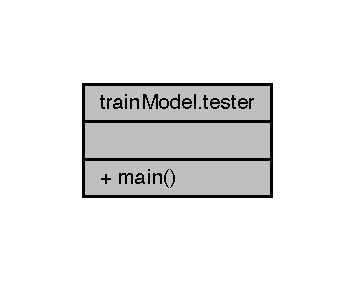
\includegraphics[width=170pt]{classtrainModel_1_1tester__coll__graph}
\end{center}
\end{figure}
\subsection*{Static Public Member Functions}
\begin{DoxyCompactItemize}
\item 
static void \hyperlink{classtrainModel_1_1tester_afd279d1cabc1e22c8e7c537266f3b0ad}{main} (String\mbox{[}$\,$\mbox{]} args)
\end{DoxyCompactItemize}


\subsection{Member Function Documentation}
\mbox{\Hypertarget{classtrainModel_1_1tester_afd279d1cabc1e22c8e7c537266f3b0ad}\label{classtrainModel_1_1tester_afd279d1cabc1e22c8e7c537266f3b0ad}} 
\index{train\+Model\+::tester@{train\+Model\+::tester}!main@{main}}
\index{main@{main}!train\+Model\+::tester@{train\+Model\+::tester}}
\subsubsection{\texorpdfstring{main()}{main()}}
{\footnotesize\ttfamily static void train\+Model.\+tester.\+main (\begin{DoxyParamCaption}\item[{String \mbox{[}$\,$\mbox{]}}]{args }\end{DoxyParamCaption})\hspace{0.3cm}{\ttfamily [static]}}



The documentation for this class was generated from the following file\+:\begin{DoxyCompactItemize}
\item 
src/main/java/train\+Model/\hyperlink{tester_8java}{tester.\+java}\end{DoxyCompactItemize}

\hypertarget{classWaysideController_1_1testPopUp}{}\section{Wayside\+Controller.\+test\+Pop\+Up Class Reference}
\label{classWaysideController_1_1testPopUp}\index{Wayside\+Controller.\+test\+Pop\+Up@{Wayside\+Controller.\+test\+Pop\+Up}}


Collaboration diagram for Wayside\+Controller.\+test\+Pop\+Up\+:
\nopagebreak
\begin{figure}[H]
\begin{center}
\leavevmode
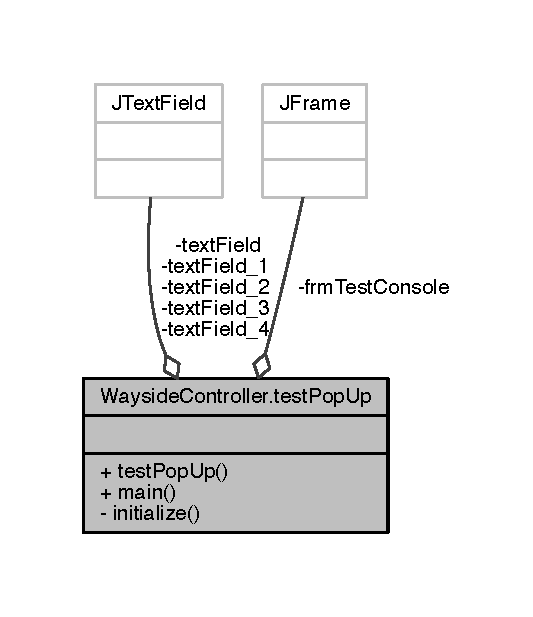
\includegraphics[width=256pt]{classWaysideController_1_1testPopUp__coll__graph}
\end{center}
\end{figure}
\subsection*{Public Member Functions}
\begin{DoxyCompactItemize}
\item 
\hyperlink{classWaysideController_1_1testPopUp_aca786bae3886bcc67ee27de840713e80}{test\+Pop\+Up} ()
\begin{DoxyCompactList}\small\item\em Create the application. \end{DoxyCompactList}\end{DoxyCompactItemize}
\subsection*{Static Public Member Functions}
\begin{DoxyCompactItemize}
\item 
static void \hyperlink{classWaysideController_1_1testPopUp_ac54f2c2c1dbe5aa8a76375e714641124}{main} (String\mbox{[}$\,$\mbox{]} args)
\begin{DoxyCompactList}\small\item\em Launch the application. \end{DoxyCompactList}\end{DoxyCompactItemize}
\subsection*{Private Member Functions}
\begin{DoxyCompactItemize}
\item 
void \hyperlink{classWaysideController_1_1testPopUp_a70581bc9a4295357f7a7ad313c6a0568}{initialize} ()
\begin{DoxyCompactList}\small\item\em Initialize the contents of the frame. \end{DoxyCompactList}\end{DoxyCompactItemize}
\subsection*{Private Attributes}
\begin{DoxyCompactItemize}
\item 
J\+Frame \hyperlink{classWaysideController_1_1testPopUp_ab508198c90a80563589466ef9e44d97e}{frm\+Test\+Console}
\item 
J\+Text\+Field \hyperlink{classWaysideController_1_1testPopUp_a514c5f48db1808eb635d27a88533964e}{text\+Field}
\item 
J\+Text\+Field \hyperlink{classWaysideController_1_1testPopUp_a4132217526e4a0f097cf97c2f5673709}{text\+Field\+\_\+1}
\item 
J\+Text\+Field \hyperlink{classWaysideController_1_1testPopUp_a87ff222532769e488dee14997c260e16}{text\+Field\+\_\+2}
\item 
J\+Text\+Field \hyperlink{classWaysideController_1_1testPopUp_ad354a48b6af395820d0edea84f8269d8}{text\+Field\+\_\+3}
\item 
J\+Text\+Field \hyperlink{classWaysideController_1_1testPopUp_af541d3ad7b2176e774fe32456d440ec9}{text\+Field\+\_\+4}
\end{DoxyCompactItemize}


\subsection{Constructor \& Destructor Documentation}
\mbox{\Hypertarget{classWaysideController_1_1testPopUp_aca786bae3886bcc67ee27de840713e80}\label{classWaysideController_1_1testPopUp_aca786bae3886bcc67ee27de840713e80}} 
\index{Wayside\+Controller\+::test\+Pop\+Up@{Wayside\+Controller\+::test\+Pop\+Up}!test\+Pop\+Up@{test\+Pop\+Up}}
\index{test\+Pop\+Up@{test\+Pop\+Up}!Wayside\+Controller\+::test\+Pop\+Up@{Wayside\+Controller\+::test\+Pop\+Up}}
\subsubsection{\texorpdfstring{test\+Pop\+Up()}{testPopUp()}}
{\footnotesize\ttfamily Wayside\+Controller.\+test\+Pop\+Up.\+test\+Pop\+Up (\begin{DoxyParamCaption}{ }\end{DoxyParamCaption})}



Create the application. 



\subsection{Member Function Documentation}
\mbox{\Hypertarget{classWaysideController_1_1testPopUp_a70581bc9a4295357f7a7ad313c6a0568}\label{classWaysideController_1_1testPopUp_a70581bc9a4295357f7a7ad313c6a0568}} 
\index{Wayside\+Controller\+::test\+Pop\+Up@{Wayside\+Controller\+::test\+Pop\+Up}!initialize@{initialize}}
\index{initialize@{initialize}!Wayside\+Controller\+::test\+Pop\+Up@{Wayside\+Controller\+::test\+Pop\+Up}}
\subsubsection{\texorpdfstring{initialize()}{initialize()}}
{\footnotesize\ttfamily void Wayside\+Controller.\+test\+Pop\+Up.\+initialize (\begin{DoxyParamCaption}{ }\end{DoxyParamCaption})\hspace{0.3cm}{\ttfamily [private]}}



Initialize the contents of the frame. 

\mbox{\Hypertarget{classWaysideController_1_1testPopUp_ac54f2c2c1dbe5aa8a76375e714641124}\label{classWaysideController_1_1testPopUp_ac54f2c2c1dbe5aa8a76375e714641124}} 
\index{Wayside\+Controller\+::test\+Pop\+Up@{Wayside\+Controller\+::test\+Pop\+Up}!main@{main}}
\index{main@{main}!Wayside\+Controller\+::test\+Pop\+Up@{Wayside\+Controller\+::test\+Pop\+Up}}
\subsubsection{\texorpdfstring{main()}{main()}}
{\footnotesize\ttfamily static void Wayside\+Controller.\+test\+Pop\+Up.\+main (\begin{DoxyParamCaption}\item[{String \mbox{[}$\,$\mbox{]}}]{args }\end{DoxyParamCaption})\hspace{0.3cm}{\ttfamily [static]}}



Launch the application. 



\subsection{Member Data Documentation}
\mbox{\Hypertarget{classWaysideController_1_1testPopUp_ab508198c90a80563589466ef9e44d97e}\label{classWaysideController_1_1testPopUp_ab508198c90a80563589466ef9e44d97e}} 
\index{Wayside\+Controller\+::test\+Pop\+Up@{Wayside\+Controller\+::test\+Pop\+Up}!frm\+Test\+Console@{frm\+Test\+Console}}
\index{frm\+Test\+Console@{frm\+Test\+Console}!Wayside\+Controller\+::test\+Pop\+Up@{Wayside\+Controller\+::test\+Pop\+Up}}
\subsubsection{\texorpdfstring{frm\+Test\+Console}{frmTestConsole}}
{\footnotesize\ttfamily J\+Frame Wayside\+Controller.\+test\+Pop\+Up.\+frm\+Test\+Console\hspace{0.3cm}{\ttfamily [private]}}

\mbox{\Hypertarget{classWaysideController_1_1testPopUp_a514c5f48db1808eb635d27a88533964e}\label{classWaysideController_1_1testPopUp_a514c5f48db1808eb635d27a88533964e}} 
\index{Wayside\+Controller\+::test\+Pop\+Up@{Wayside\+Controller\+::test\+Pop\+Up}!text\+Field@{text\+Field}}
\index{text\+Field@{text\+Field}!Wayside\+Controller\+::test\+Pop\+Up@{Wayside\+Controller\+::test\+Pop\+Up}}
\subsubsection{\texorpdfstring{text\+Field}{textField}}
{\footnotesize\ttfamily J\+Text\+Field Wayside\+Controller.\+test\+Pop\+Up.\+text\+Field\hspace{0.3cm}{\ttfamily [private]}}

\mbox{\Hypertarget{classWaysideController_1_1testPopUp_a4132217526e4a0f097cf97c2f5673709}\label{classWaysideController_1_1testPopUp_a4132217526e4a0f097cf97c2f5673709}} 
\index{Wayside\+Controller\+::test\+Pop\+Up@{Wayside\+Controller\+::test\+Pop\+Up}!text\+Field\+\_\+1@{text\+Field\+\_\+1}}
\index{text\+Field\+\_\+1@{text\+Field\+\_\+1}!Wayside\+Controller\+::test\+Pop\+Up@{Wayside\+Controller\+::test\+Pop\+Up}}
\subsubsection{\texorpdfstring{text\+Field\+\_\+1}{textField\_1}}
{\footnotesize\ttfamily J\+Text\+Field Wayside\+Controller.\+test\+Pop\+Up.\+text\+Field\+\_\+1\hspace{0.3cm}{\ttfamily [private]}}

\mbox{\Hypertarget{classWaysideController_1_1testPopUp_a87ff222532769e488dee14997c260e16}\label{classWaysideController_1_1testPopUp_a87ff222532769e488dee14997c260e16}} 
\index{Wayside\+Controller\+::test\+Pop\+Up@{Wayside\+Controller\+::test\+Pop\+Up}!text\+Field\+\_\+2@{text\+Field\+\_\+2}}
\index{text\+Field\+\_\+2@{text\+Field\+\_\+2}!Wayside\+Controller\+::test\+Pop\+Up@{Wayside\+Controller\+::test\+Pop\+Up}}
\subsubsection{\texorpdfstring{text\+Field\+\_\+2}{textField\_2}}
{\footnotesize\ttfamily J\+Text\+Field Wayside\+Controller.\+test\+Pop\+Up.\+text\+Field\+\_\+2\hspace{0.3cm}{\ttfamily [private]}}

\mbox{\Hypertarget{classWaysideController_1_1testPopUp_ad354a48b6af395820d0edea84f8269d8}\label{classWaysideController_1_1testPopUp_ad354a48b6af395820d0edea84f8269d8}} 
\index{Wayside\+Controller\+::test\+Pop\+Up@{Wayside\+Controller\+::test\+Pop\+Up}!text\+Field\+\_\+3@{text\+Field\+\_\+3}}
\index{text\+Field\+\_\+3@{text\+Field\+\_\+3}!Wayside\+Controller\+::test\+Pop\+Up@{Wayside\+Controller\+::test\+Pop\+Up}}
\subsubsection{\texorpdfstring{text\+Field\+\_\+3}{textField\_3}}
{\footnotesize\ttfamily J\+Text\+Field Wayside\+Controller.\+test\+Pop\+Up.\+text\+Field\+\_\+3\hspace{0.3cm}{\ttfamily [private]}}

\mbox{\Hypertarget{classWaysideController_1_1testPopUp_af541d3ad7b2176e774fe32456d440ec9}\label{classWaysideController_1_1testPopUp_af541d3ad7b2176e774fe32456d440ec9}} 
\index{Wayside\+Controller\+::test\+Pop\+Up@{Wayside\+Controller\+::test\+Pop\+Up}!text\+Field\+\_\+4@{text\+Field\+\_\+4}}
\index{text\+Field\+\_\+4@{text\+Field\+\_\+4}!Wayside\+Controller\+::test\+Pop\+Up@{Wayside\+Controller\+::test\+Pop\+Up}}
\subsubsection{\texorpdfstring{text\+Field\+\_\+4}{textField\_4}}
{\footnotesize\ttfamily J\+Text\+Field Wayside\+Controller.\+test\+Pop\+Up.\+text\+Field\+\_\+4\hspace{0.3cm}{\ttfamily [private]}}



The documentation for this class was generated from the following file\+:\begin{DoxyCompactItemize}
\item 
src/main/java/\+Wayside\+Controller/\hyperlink{testPopUp_8java}{test\+Pop\+Up.\+java}\end{DoxyCompactItemize}

\hypertarget{classTrainControllerComps_1_1TestTrain}{}\section{Train\+Controller\+Comps.\+Test\+Train Class Reference}
\label{classTrainControllerComps_1_1TestTrain}\index{Train\+Controller\+Comps.\+Test\+Train@{Train\+Controller\+Comps.\+Test\+Train}}


Collaboration diagram for Train\+Controller\+Comps.\+Test\+Train\+:
\nopagebreak
\begin{figure}[H]
\begin{center}
\leavevmode
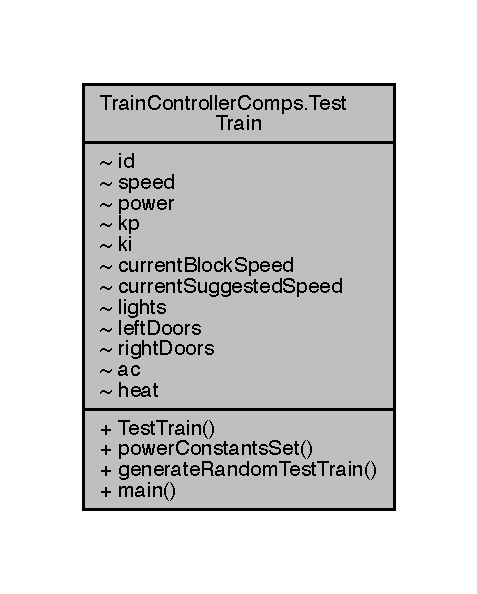
\includegraphics[width=229pt]{classTrainControllerComps_1_1TestTrain__coll__graph}
\end{center}
\end{figure}
\subsection*{Public Member Functions}
\begin{DoxyCompactItemize}
\item 
\hyperlink{classTrainControllerComps_1_1TestTrain_abf782fec0223ecf2fbf046fa4a8c5053}{Test\+Train} (String \hyperlink{classTrainControllerComps_1_1TestTrain_a9e1acb4fe54e1d3cebdbf45aa70c74b3}{id})
\item 
boolean \hyperlink{classTrainControllerComps_1_1TestTrain_aeae0e0501dad3d4529679d01c7baca6b}{power\+Constants\+Set} ()
\end{DoxyCompactItemize}
\subsection*{Static Public Member Functions}
\begin{DoxyCompactItemize}
\item 
static Linked\+List$<$ \hyperlink{classTrainControllerComps_1_1TestTrain}{Test\+Train} $>$ \hyperlink{classTrainControllerComps_1_1TestTrain_a9ac49f75c523af590e04e6feec2b2b0d}{generate\+Random\+Test\+Train} (int how\+Many)
\begin{DoxyCompactList}\small\item\em Generates \textquotesingle{}how\+Many\textquotesingle{} number of Test\+Trains, and assigns a random Speed and Power. \end{DoxyCompactList}\item 
static void \hyperlink{classTrainControllerComps_1_1TestTrain_abcd04903f3a72e1cc2c667edfc3930ec}{main} (String\mbox{[}$\,$\mbox{]} args)
\end{DoxyCompactItemize}
\subsection*{Package Attributes}
\begin{DoxyCompactItemize}
\item 
String \hyperlink{classTrainControllerComps_1_1TestTrain_a9e1acb4fe54e1d3cebdbf45aa70c74b3}{id}
\item 
double \hyperlink{classTrainControllerComps_1_1TestTrain_a9904816560b86c2fc9a9c9674139e37d}{speed}
\item 
double \hyperlink{classTrainControllerComps_1_1TestTrain_a8416b4c7dced6baaf6437737d6442401}{power}
\item 
Double \hyperlink{classTrainControllerComps_1_1TestTrain_a89626f4debafbbd7bedf7832bec55711}{kp}
\item 
Double \hyperlink{classTrainControllerComps_1_1TestTrain_acfaf0a5760dbfcaaa6b19a5f950df7d4}{ki}
\item 
double \hyperlink{classTrainControllerComps_1_1TestTrain_a759a319845a8467052c55f38e15a10c3}{current\+Block\+Speed}
\item 
double \hyperlink{classTrainControllerComps_1_1TestTrain_aff2417885f562dc95f9ecff931a49180}{current\+Suggested\+Speed}
\item 
int \hyperlink{classTrainControllerComps_1_1TestTrain_ab04e07e68d782f16a352d6034baab648}{lights}
\item 
int \hyperlink{classTrainControllerComps_1_1TestTrain_a7b99e5d746f86203da443ad7bcc8bbde}{left\+Doors}
\item 
int \hyperlink{classTrainControllerComps_1_1TestTrain_a87496df76f82b4f0736afdcd60b42e0e}{right\+Doors}
\item 
int \hyperlink{classTrainControllerComps_1_1TestTrain_a65cb0b4b1944821c9b71f53167a57ec7}{ac}
\item 
int \hyperlink{classTrainControllerComps_1_1TestTrain_a31ee8bfd0d2b333df692583a26eed6a5}{heat}
\end{DoxyCompactItemize}


\subsection{Detailed Description}
\begin{DoxyAuthor}{Author}
Andrew 
\end{DoxyAuthor}


\subsection{Constructor \& Destructor Documentation}
\mbox{\Hypertarget{classTrainControllerComps_1_1TestTrain_abf782fec0223ecf2fbf046fa4a8c5053}\label{classTrainControllerComps_1_1TestTrain_abf782fec0223ecf2fbf046fa4a8c5053}} 
\index{Train\+Controller\+Comps\+::\+Test\+Train@{Train\+Controller\+Comps\+::\+Test\+Train}!Test\+Train@{Test\+Train}}
\index{Test\+Train@{Test\+Train}!Train\+Controller\+Comps\+::\+Test\+Train@{Train\+Controller\+Comps\+::\+Test\+Train}}
\subsubsection{\texorpdfstring{Test\+Train()}{TestTrain()}}
{\footnotesize\ttfamily Train\+Controller\+Comps.\+Test\+Train.\+Test\+Train (\begin{DoxyParamCaption}\item[{String}]{id }\end{DoxyParamCaption})}



\subsection{Member Function Documentation}
\mbox{\Hypertarget{classTrainControllerComps_1_1TestTrain_a9ac49f75c523af590e04e6feec2b2b0d}\label{classTrainControllerComps_1_1TestTrain_a9ac49f75c523af590e04e6feec2b2b0d}} 
\index{Train\+Controller\+Comps\+::\+Test\+Train@{Train\+Controller\+Comps\+::\+Test\+Train}!generate\+Random\+Test\+Train@{generate\+Random\+Test\+Train}}
\index{generate\+Random\+Test\+Train@{generate\+Random\+Test\+Train}!Train\+Controller\+Comps\+::\+Test\+Train@{Train\+Controller\+Comps\+::\+Test\+Train}}
\subsubsection{\texorpdfstring{generate\+Random\+Test\+Train()}{generateRandomTestTrain()}}
{\footnotesize\ttfamily static Linked\+List$<$\hyperlink{classTrainControllerComps_1_1TestTrain}{Test\+Train}$>$ Train\+Controller\+Comps.\+Test\+Train.\+generate\+Random\+Test\+Train (\begin{DoxyParamCaption}\item[{int}]{how\+Many }\end{DoxyParamCaption})\hspace{0.3cm}{\ttfamily [static]}}



Generates \textquotesingle{}how\+Many\textquotesingle{} number of Test\+Trains, and assigns a random Speed and Power. 


\begin{DoxyParams}{Parameters}
{\em how\+Many} & the number of trains you want to generate \\
\hline
\end{DoxyParams}
\begin{DoxyReturn}{Returns}
A list containing \textquotesingle{}how\+Many\textquotesingle{} \hyperlink{classTrainControllerComps_1_1TestTrain}{Test\+Train} objects. 
\end{DoxyReturn}
\mbox{\Hypertarget{classTrainControllerComps_1_1TestTrain_abcd04903f3a72e1cc2c667edfc3930ec}\label{classTrainControllerComps_1_1TestTrain_abcd04903f3a72e1cc2c667edfc3930ec}} 
\index{Train\+Controller\+Comps\+::\+Test\+Train@{Train\+Controller\+Comps\+::\+Test\+Train}!main@{main}}
\index{main@{main}!Train\+Controller\+Comps\+::\+Test\+Train@{Train\+Controller\+Comps\+::\+Test\+Train}}
\subsubsection{\texorpdfstring{main()}{main()}}
{\footnotesize\ttfamily static void Train\+Controller\+Comps.\+Test\+Train.\+main (\begin{DoxyParamCaption}\item[{String \mbox{[}$\,$\mbox{]}}]{args }\end{DoxyParamCaption})\hspace{0.3cm}{\ttfamily [static]}}

\mbox{\Hypertarget{classTrainControllerComps_1_1TestTrain_aeae0e0501dad3d4529679d01c7baca6b}\label{classTrainControllerComps_1_1TestTrain_aeae0e0501dad3d4529679d01c7baca6b}} 
\index{Train\+Controller\+Comps\+::\+Test\+Train@{Train\+Controller\+Comps\+::\+Test\+Train}!power\+Constants\+Set@{power\+Constants\+Set}}
\index{power\+Constants\+Set@{power\+Constants\+Set}!Train\+Controller\+Comps\+::\+Test\+Train@{Train\+Controller\+Comps\+::\+Test\+Train}}
\subsubsection{\texorpdfstring{power\+Constants\+Set()}{powerConstantsSet()}}
{\footnotesize\ttfamily boolean Train\+Controller\+Comps.\+Test\+Train.\+power\+Constants\+Set (\begin{DoxyParamCaption}{ }\end{DoxyParamCaption})}



\subsection{Member Data Documentation}
\mbox{\Hypertarget{classTrainControllerComps_1_1TestTrain_a65cb0b4b1944821c9b71f53167a57ec7}\label{classTrainControllerComps_1_1TestTrain_a65cb0b4b1944821c9b71f53167a57ec7}} 
\index{Train\+Controller\+Comps\+::\+Test\+Train@{Train\+Controller\+Comps\+::\+Test\+Train}!ac@{ac}}
\index{ac@{ac}!Train\+Controller\+Comps\+::\+Test\+Train@{Train\+Controller\+Comps\+::\+Test\+Train}}
\subsubsection{\texorpdfstring{ac}{ac}}
{\footnotesize\ttfamily int Train\+Controller\+Comps.\+Test\+Train.\+ac\hspace{0.3cm}{\ttfamily [package]}}

\mbox{\Hypertarget{classTrainControllerComps_1_1TestTrain_a759a319845a8467052c55f38e15a10c3}\label{classTrainControllerComps_1_1TestTrain_a759a319845a8467052c55f38e15a10c3}} 
\index{Train\+Controller\+Comps\+::\+Test\+Train@{Train\+Controller\+Comps\+::\+Test\+Train}!current\+Block\+Speed@{current\+Block\+Speed}}
\index{current\+Block\+Speed@{current\+Block\+Speed}!Train\+Controller\+Comps\+::\+Test\+Train@{Train\+Controller\+Comps\+::\+Test\+Train}}
\subsubsection{\texorpdfstring{current\+Block\+Speed}{currentBlockSpeed}}
{\footnotesize\ttfamily double Train\+Controller\+Comps.\+Test\+Train.\+current\+Block\+Speed\hspace{0.3cm}{\ttfamily [package]}}

\mbox{\Hypertarget{classTrainControllerComps_1_1TestTrain_aff2417885f562dc95f9ecff931a49180}\label{classTrainControllerComps_1_1TestTrain_aff2417885f562dc95f9ecff931a49180}} 
\index{Train\+Controller\+Comps\+::\+Test\+Train@{Train\+Controller\+Comps\+::\+Test\+Train}!current\+Suggested\+Speed@{current\+Suggested\+Speed}}
\index{current\+Suggested\+Speed@{current\+Suggested\+Speed}!Train\+Controller\+Comps\+::\+Test\+Train@{Train\+Controller\+Comps\+::\+Test\+Train}}
\subsubsection{\texorpdfstring{current\+Suggested\+Speed}{currentSuggestedSpeed}}
{\footnotesize\ttfamily double Train\+Controller\+Comps.\+Test\+Train.\+current\+Suggested\+Speed\hspace{0.3cm}{\ttfamily [package]}}

\mbox{\Hypertarget{classTrainControllerComps_1_1TestTrain_a31ee8bfd0d2b333df692583a26eed6a5}\label{classTrainControllerComps_1_1TestTrain_a31ee8bfd0d2b333df692583a26eed6a5}} 
\index{Train\+Controller\+Comps\+::\+Test\+Train@{Train\+Controller\+Comps\+::\+Test\+Train}!heat@{heat}}
\index{heat@{heat}!Train\+Controller\+Comps\+::\+Test\+Train@{Train\+Controller\+Comps\+::\+Test\+Train}}
\subsubsection{\texorpdfstring{heat}{heat}}
{\footnotesize\ttfamily int Train\+Controller\+Comps.\+Test\+Train.\+heat\hspace{0.3cm}{\ttfamily [package]}}

\mbox{\Hypertarget{classTrainControllerComps_1_1TestTrain_a9e1acb4fe54e1d3cebdbf45aa70c74b3}\label{classTrainControllerComps_1_1TestTrain_a9e1acb4fe54e1d3cebdbf45aa70c74b3}} 
\index{Train\+Controller\+Comps\+::\+Test\+Train@{Train\+Controller\+Comps\+::\+Test\+Train}!id@{id}}
\index{id@{id}!Train\+Controller\+Comps\+::\+Test\+Train@{Train\+Controller\+Comps\+::\+Test\+Train}}
\subsubsection{\texorpdfstring{id}{id}}
{\footnotesize\ttfamily String Train\+Controller\+Comps.\+Test\+Train.\+id\hspace{0.3cm}{\ttfamily [package]}}

\mbox{\Hypertarget{classTrainControllerComps_1_1TestTrain_acfaf0a5760dbfcaaa6b19a5f950df7d4}\label{classTrainControllerComps_1_1TestTrain_acfaf0a5760dbfcaaa6b19a5f950df7d4}} 
\index{Train\+Controller\+Comps\+::\+Test\+Train@{Train\+Controller\+Comps\+::\+Test\+Train}!ki@{ki}}
\index{ki@{ki}!Train\+Controller\+Comps\+::\+Test\+Train@{Train\+Controller\+Comps\+::\+Test\+Train}}
\subsubsection{\texorpdfstring{ki}{ki}}
{\footnotesize\ttfamily Double Train\+Controller\+Comps.\+Test\+Train.\+ki\hspace{0.3cm}{\ttfamily [package]}}

\mbox{\Hypertarget{classTrainControllerComps_1_1TestTrain_a89626f4debafbbd7bedf7832bec55711}\label{classTrainControllerComps_1_1TestTrain_a89626f4debafbbd7bedf7832bec55711}} 
\index{Train\+Controller\+Comps\+::\+Test\+Train@{Train\+Controller\+Comps\+::\+Test\+Train}!kp@{kp}}
\index{kp@{kp}!Train\+Controller\+Comps\+::\+Test\+Train@{Train\+Controller\+Comps\+::\+Test\+Train}}
\subsubsection{\texorpdfstring{kp}{kp}}
{\footnotesize\ttfamily Double Train\+Controller\+Comps.\+Test\+Train.\+kp\hspace{0.3cm}{\ttfamily [package]}}

\mbox{\Hypertarget{classTrainControllerComps_1_1TestTrain_a7b99e5d746f86203da443ad7bcc8bbde}\label{classTrainControllerComps_1_1TestTrain_a7b99e5d746f86203da443ad7bcc8bbde}} 
\index{Train\+Controller\+Comps\+::\+Test\+Train@{Train\+Controller\+Comps\+::\+Test\+Train}!left\+Doors@{left\+Doors}}
\index{left\+Doors@{left\+Doors}!Train\+Controller\+Comps\+::\+Test\+Train@{Train\+Controller\+Comps\+::\+Test\+Train}}
\subsubsection{\texorpdfstring{left\+Doors}{leftDoors}}
{\footnotesize\ttfamily int Train\+Controller\+Comps.\+Test\+Train.\+left\+Doors\hspace{0.3cm}{\ttfamily [package]}}

\mbox{\Hypertarget{classTrainControllerComps_1_1TestTrain_ab04e07e68d782f16a352d6034baab648}\label{classTrainControllerComps_1_1TestTrain_ab04e07e68d782f16a352d6034baab648}} 
\index{Train\+Controller\+Comps\+::\+Test\+Train@{Train\+Controller\+Comps\+::\+Test\+Train}!lights@{lights}}
\index{lights@{lights}!Train\+Controller\+Comps\+::\+Test\+Train@{Train\+Controller\+Comps\+::\+Test\+Train}}
\subsubsection{\texorpdfstring{lights}{lights}}
{\footnotesize\ttfamily int Train\+Controller\+Comps.\+Test\+Train.\+lights\hspace{0.3cm}{\ttfamily [package]}}

\mbox{\Hypertarget{classTrainControllerComps_1_1TestTrain_a8416b4c7dced6baaf6437737d6442401}\label{classTrainControllerComps_1_1TestTrain_a8416b4c7dced6baaf6437737d6442401}} 
\index{Train\+Controller\+Comps\+::\+Test\+Train@{Train\+Controller\+Comps\+::\+Test\+Train}!power@{power}}
\index{power@{power}!Train\+Controller\+Comps\+::\+Test\+Train@{Train\+Controller\+Comps\+::\+Test\+Train}}
\subsubsection{\texorpdfstring{power}{power}}
{\footnotesize\ttfamily double Train\+Controller\+Comps.\+Test\+Train.\+power\hspace{0.3cm}{\ttfamily [package]}}

\mbox{\Hypertarget{classTrainControllerComps_1_1TestTrain_a87496df76f82b4f0736afdcd60b42e0e}\label{classTrainControllerComps_1_1TestTrain_a87496df76f82b4f0736afdcd60b42e0e}} 
\index{Train\+Controller\+Comps\+::\+Test\+Train@{Train\+Controller\+Comps\+::\+Test\+Train}!right\+Doors@{right\+Doors}}
\index{right\+Doors@{right\+Doors}!Train\+Controller\+Comps\+::\+Test\+Train@{Train\+Controller\+Comps\+::\+Test\+Train}}
\subsubsection{\texorpdfstring{right\+Doors}{rightDoors}}
{\footnotesize\ttfamily int Train\+Controller\+Comps.\+Test\+Train.\+right\+Doors\hspace{0.3cm}{\ttfamily [package]}}

\mbox{\Hypertarget{classTrainControllerComps_1_1TestTrain_a9904816560b86c2fc9a9c9674139e37d}\label{classTrainControllerComps_1_1TestTrain_a9904816560b86c2fc9a9c9674139e37d}} 
\index{Train\+Controller\+Comps\+::\+Test\+Train@{Train\+Controller\+Comps\+::\+Test\+Train}!speed@{speed}}
\index{speed@{speed}!Train\+Controller\+Comps\+::\+Test\+Train@{Train\+Controller\+Comps\+::\+Test\+Train}}
\subsubsection{\texorpdfstring{speed}{speed}}
{\footnotesize\ttfamily double Train\+Controller\+Comps.\+Test\+Train.\+speed\hspace{0.3cm}{\ttfamily [package]}}



The documentation for this class was generated from the following file\+:\begin{DoxyCompactItemize}
\item 
src/main/java/\+Train\+Controller\+Comps/\hyperlink{TestTrain_8java}{Test\+Train.\+java}\end{DoxyCompactItemize}

\hypertarget{classtrackDetails}{}\section{track\+Details Class Reference}
\label{classtrackDetails}\index{track\+Details@{track\+Details}}


Collaboration diagram for track\+Details\+:
\nopagebreak
\begin{figure}[H]
\begin{center}
\leavevmode
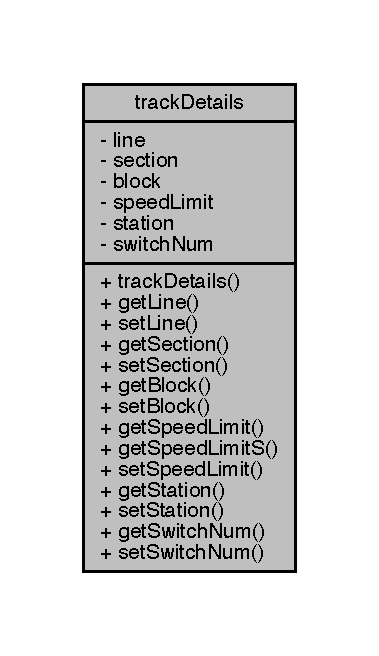
\includegraphics[width=182pt]{classtrackDetails__coll__graph}
\end{center}
\end{figure}
\subsection*{Public Member Functions}
\begin{DoxyCompactItemize}
\item 
\hyperlink{classtrackDetails_a3cae5dfd3207dce4756ce2f0353a5763}{track\+Details} (String \hyperlink{classtrackDetails_a8b79c0cfb50c7468da12fa27136ad405}{line}, String \hyperlink{classtrackDetails_ab792824f4e3b7a384dd6edd2477a71e4}{section}, int \hyperlink{classtrackDetails_a13669b99469f4b78df534fbb72f4143d}{block}, double \hyperlink{classtrackDetails_a1d5bd79ee0bb744bec31e83a3d2895dd}{speed\+Limit}, String \hyperlink{classtrackDetails_ac7e67717763b308bcab1b1103f9aa1f7}{station}, String \hyperlink{classtrackDetails_a505f97a602c160591e64664790ca4e5b}{switch\+Num})
\item 
String \hyperlink{classtrackDetails_a1d44908db14b13943285cb96a2650f39}{get\+Line} ()
\item 
void \hyperlink{classtrackDetails_a4d6a369eef1fac06475277177369d6a3}{set\+Line} (String \hyperlink{classtrackDetails_a8b79c0cfb50c7468da12fa27136ad405}{line})
\item 
String \hyperlink{classtrackDetails_a6015cc578bd221d08f86e7149bc628d4}{get\+Section} ()
\item 
void \hyperlink{classtrackDetails_a7eaba9d9e69088bec45012a062fa594a}{set\+Section} (String \hyperlink{classtrackDetails_ab792824f4e3b7a384dd6edd2477a71e4}{section})
\item 
int \hyperlink{classtrackDetails_ace170128a164913c83f3cba25dda135f}{get\+Block} ()
\item 
void \hyperlink{classtrackDetails_a156625126ad75671296575c9abb60299}{set\+Block} (int \hyperlink{classtrackDetails_a13669b99469f4b78df534fbb72f4143d}{block})
\item 
double \hyperlink{classtrackDetails_ad98f82166c38d18a0b5ce5b58f302a35}{get\+Speed\+Limit} ()
\item 
String \hyperlink{classtrackDetails_a8857c7e4a957d7fe39d1e38dc090f3e1}{get\+Speed\+LimitS} (double \hyperlink{classtrackDetails_a1d5bd79ee0bb744bec31e83a3d2895dd}{speed\+Limit})
\item 
void \hyperlink{classtrackDetails_a0b6bfc44b0d1613b769fb77c8fcb70b3}{set\+Speed\+Limit} (double \hyperlink{classtrackDetails_a1d5bd79ee0bb744bec31e83a3d2895dd}{speed\+Limit})
\item 
String \hyperlink{classtrackDetails_af4717e6aa7ccfa4e5e477d61a58b0830}{get\+Station} ()
\item 
void \hyperlink{classtrackDetails_a55dc6c094eaf9091c40f88c570bb5964}{set\+Station} (String \hyperlink{classtrackDetails_ac7e67717763b308bcab1b1103f9aa1f7}{station})
\item 
String \hyperlink{classtrackDetails_af3e64ab27ae22ea6db064dca52da01ea}{get\+Switch\+Num} ()
\item 
void \hyperlink{classtrackDetails_a12c839239d3bf567b166ad5e71dd88b7}{set\+Switch\+Num} (String \hyperlink{classtrackDetails_a505f97a602c160591e64664790ca4e5b}{switch\+Num})
\end{DoxyCompactItemize}
\subsection*{Private Attributes}
\begin{DoxyCompactItemize}
\item 
String \hyperlink{classtrackDetails_a8b79c0cfb50c7468da12fa27136ad405}{line}
\item 
String \hyperlink{classtrackDetails_ab792824f4e3b7a384dd6edd2477a71e4}{section}
\item 
int \hyperlink{classtrackDetails_a13669b99469f4b78df534fbb72f4143d}{block}
\item 
double \hyperlink{classtrackDetails_a1d5bd79ee0bb744bec31e83a3d2895dd}{speed\+Limit}
\item 
String \hyperlink{classtrackDetails_ac7e67717763b308bcab1b1103f9aa1f7}{station}
\item 
String \hyperlink{classtrackDetails_a505f97a602c160591e64664790ca4e5b}{switch\+Num}
\end{DoxyCompactItemize}


\subsection{Constructor \& Destructor Documentation}
\mbox{\Hypertarget{classtrackDetails_a3cae5dfd3207dce4756ce2f0353a5763}\label{classtrackDetails_a3cae5dfd3207dce4756ce2f0353a5763}} 
\index{track\+Details@{track\+Details}!track\+Details@{track\+Details}}
\index{track\+Details@{track\+Details}!track\+Details@{track\+Details}}
\subsubsection{\texorpdfstring{track\+Details()}{trackDetails()}}
{\footnotesize\ttfamily track\+Details.\+track\+Details (\begin{DoxyParamCaption}\item[{String}]{line,  }\item[{String}]{section,  }\item[{int}]{block,  }\item[{double}]{speed\+Limit,  }\item[{String}]{station,  }\item[{String}]{switch\+Num }\end{DoxyParamCaption})}



\subsection{Member Function Documentation}
\mbox{\Hypertarget{classtrackDetails_ace170128a164913c83f3cba25dda135f}\label{classtrackDetails_ace170128a164913c83f3cba25dda135f}} 
\index{track\+Details@{track\+Details}!get\+Block@{get\+Block}}
\index{get\+Block@{get\+Block}!track\+Details@{track\+Details}}
\subsubsection{\texorpdfstring{get\+Block()}{getBlock()}}
{\footnotesize\ttfamily int track\+Details.\+get\+Block (\begin{DoxyParamCaption}{ }\end{DoxyParamCaption})}

\mbox{\Hypertarget{classtrackDetails_a1d44908db14b13943285cb96a2650f39}\label{classtrackDetails_a1d44908db14b13943285cb96a2650f39}} 
\index{track\+Details@{track\+Details}!get\+Line@{get\+Line}}
\index{get\+Line@{get\+Line}!track\+Details@{track\+Details}}
\subsubsection{\texorpdfstring{get\+Line()}{getLine()}}
{\footnotesize\ttfamily String track\+Details.\+get\+Line (\begin{DoxyParamCaption}{ }\end{DoxyParamCaption})}

\mbox{\Hypertarget{classtrackDetails_a6015cc578bd221d08f86e7149bc628d4}\label{classtrackDetails_a6015cc578bd221d08f86e7149bc628d4}} 
\index{track\+Details@{track\+Details}!get\+Section@{get\+Section}}
\index{get\+Section@{get\+Section}!track\+Details@{track\+Details}}
\subsubsection{\texorpdfstring{get\+Section()}{getSection()}}
{\footnotesize\ttfamily String track\+Details.\+get\+Section (\begin{DoxyParamCaption}{ }\end{DoxyParamCaption})}

\mbox{\Hypertarget{classtrackDetails_ad98f82166c38d18a0b5ce5b58f302a35}\label{classtrackDetails_ad98f82166c38d18a0b5ce5b58f302a35}} 
\index{track\+Details@{track\+Details}!get\+Speed\+Limit@{get\+Speed\+Limit}}
\index{get\+Speed\+Limit@{get\+Speed\+Limit}!track\+Details@{track\+Details}}
\subsubsection{\texorpdfstring{get\+Speed\+Limit()}{getSpeedLimit()}}
{\footnotesize\ttfamily double track\+Details.\+get\+Speed\+Limit (\begin{DoxyParamCaption}{ }\end{DoxyParamCaption})}

\mbox{\Hypertarget{classtrackDetails_a8857c7e4a957d7fe39d1e38dc090f3e1}\label{classtrackDetails_a8857c7e4a957d7fe39d1e38dc090f3e1}} 
\index{track\+Details@{track\+Details}!get\+Speed\+LimitS@{get\+Speed\+LimitS}}
\index{get\+Speed\+LimitS@{get\+Speed\+LimitS}!track\+Details@{track\+Details}}
\subsubsection{\texorpdfstring{get\+Speed\+Limit\+S()}{getSpeedLimitS()}}
{\footnotesize\ttfamily String track\+Details.\+get\+Speed\+LimitS (\begin{DoxyParamCaption}\item[{double}]{speed\+Limit }\end{DoxyParamCaption})}

\mbox{\Hypertarget{classtrackDetails_af4717e6aa7ccfa4e5e477d61a58b0830}\label{classtrackDetails_af4717e6aa7ccfa4e5e477d61a58b0830}} 
\index{track\+Details@{track\+Details}!get\+Station@{get\+Station}}
\index{get\+Station@{get\+Station}!track\+Details@{track\+Details}}
\subsubsection{\texorpdfstring{get\+Station()}{getStation()}}
{\footnotesize\ttfamily String track\+Details.\+get\+Station (\begin{DoxyParamCaption}{ }\end{DoxyParamCaption})}

\mbox{\Hypertarget{classtrackDetails_af3e64ab27ae22ea6db064dca52da01ea}\label{classtrackDetails_af3e64ab27ae22ea6db064dca52da01ea}} 
\index{track\+Details@{track\+Details}!get\+Switch\+Num@{get\+Switch\+Num}}
\index{get\+Switch\+Num@{get\+Switch\+Num}!track\+Details@{track\+Details}}
\subsubsection{\texorpdfstring{get\+Switch\+Num()}{getSwitchNum()}}
{\footnotesize\ttfamily String track\+Details.\+get\+Switch\+Num (\begin{DoxyParamCaption}{ }\end{DoxyParamCaption})}

\mbox{\Hypertarget{classtrackDetails_a156625126ad75671296575c9abb60299}\label{classtrackDetails_a156625126ad75671296575c9abb60299}} 
\index{track\+Details@{track\+Details}!set\+Block@{set\+Block}}
\index{set\+Block@{set\+Block}!track\+Details@{track\+Details}}
\subsubsection{\texorpdfstring{set\+Block()}{setBlock()}}
{\footnotesize\ttfamily void track\+Details.\+set\+Block (\begin{DoxyParamCaption}\item[{int}]{block }\end{DoxyParamCaption})}

\mbox{\Hypertarget{classtrackDetails_a4d6a369eef1fac06475277177369d6a3}\label{classtrackDetails_a4d6a369eef1fac06475277177369d6a3}} 
\index{track\+Details@{track\+Details}!set\+Line@{set\+Line}}
\index{set\+Line@{set\+Line}!track\+Details@{track\+Details}}
\subsubsection{\texorpdfstring{set\+Line()}{setLine()}}
{\footnotesize\ttfamily void track\+Details.\+set\+Line (\begin{DoxyParamCaption}\item[{String}]{line }\end{DoxyParamCaption})}

\mbox{\Hypertarget{classtrackDetails_a7eaba9d9e69088bec45012a062fa594a}\label{classtrackDetails_a7eaba9d9e69088bec45012a062fa594a}} 
\index{track\+Details@{track\+Details}!set\+Section@{set\+Section}}
\index{set\+Section@{set\+Section}!track\+Details@{track\+Details}}
\subsubsection{\texorpdfstring{set\+Section()}{setSection()}}
{\footnotesize\ttfamily void track\+Details.\+set\+Section (\begin{DoxyParamCaption}\item[{String}]{section }\end{DoxyParamCaption})}

\mbox{\Hypertarget{classtrackDetails_a0b6bfc44b0d1613b769fb77c8fcb70b3}\label{classtrackDetails_a0b6bfc44b0d1613b769fb77c8fcb70b3}} 
\index{track\+Details@{track\+Details}!set\+Speed\+Limit@{set\+Speed\+Limit}}
\index{set\+Speed\+Limit@{set\+Speed\+Limit}!track\+Details@{track\+Details}}
\subsubsection{\texorpdfstring{set\+Speed\+Limit()}{setSpeedLimit()}}
{\footnotesize\ttfamily void track\+Details.\+set\+Speed\+Limit (\begin{DoxyParamCaption}\item[{double}]{speed\+Limit }\end{DoxyParamCaption})}

\mbox{\Hypertarget{classtrackDetails_a55dc6c094eaf9091c40f88c570bb5964}\label{classtrackDetails_a55dc6c094eaf9091c40f88c570bb5964}} 
\index{track\+Details@{track\+Details}!set\+Station@{set\+Station}}
\index{set\+Station@{set\+Station}!track\+Details@{track\+Details}}
\subsubsection{\texorpdfstring{set\+Station()}{setStation()}}
{\footnotesize\ttfamily void track\+Details.\+set\+Station (\begin{DoxyParamCaption}\item[{String}]{station }\end{DoxyParamCaption})}

\mbox{\Hypertarget{classtrackDetails_a12c839239d3bf567b166ad5e71dd88b7}\label{classtrackDetails_a12c839239d3bf567b166ad5e71dd88b7}} 
\index{track\+Details@{track\+Details}!set\+Switch\+Num@{set\+Switch\+Num}}
\index{set\+Switch\+Num@{set\+Switch\+Num}!track\+Details@{track\+Details}}
\subsubsection{\texorpdfstring{set\+Switch\+Num()}{setSwitchNum()}}
{\footnotesize\ttfamily void track\+Details.\+set\+Switch\+Num (\begin{DoxyParamCaption}\item[{String}]{switch\+Num }\end{DoxyParamCaption})}



\subsection{Member Data Documentation}
\mbox{\Hypertarget{classtrackDetails_a13669b99469f4b78df534fbb72f4143d}\label{classtrackDetails_a13669b99469f4b78df534fbb72f4143d}} 
\index{track\+Details@{track\+Details}!block@{block}}
\index{block@{block}!track\+Details@{track\+Details}}
\subsubsection{\texorpdfstring{block}{block}}
{\footnotesize\ttfamily int track\+Details.\+block\hspace{0.3cm}{\ttfamily [private]}}

\mbox{\Hypertarget{classtrackDetails_a8b79c0cfb50c7468da12fa27136ad405}\label{classtrackDetails_a8b79c0cfb50c7468da12fa27136ad405}} 
\index{track\+Details@{track\+Details}!line@{line}}
\index{line@{line}!track\+Details@{track\+Details}}
\subsubsection{\texorpdfstring{line}{line}}
{\footnotesize\ttfamily String track\+Details.\+line\hspace{0.3cm}{\ttfamily [private]}}

\mbox{\Hypertarget{classtrackDetails_ab792824f4e3b7a384dd6edd2477a71e4}\label{classtrackDetails_ab792824f4e3b7a384dd6edd2477a71e4}} 
\index{track\+Details@{track\+Details}!section@{section}}
\index{section@{section}!track\+Details@{track\+Details}}
\subsubsection{\texorpdfstring{section}{section}}
{\footnotesize\ttfamily String track\+Details.\+section\hspace{0.3cm}{\ttfamily [private]}}

\mbox{\Hypertarget{classtrackDetails_a1d5bd79ee0bb744bec31e83a3d2895dd}\label{classtrackDetails_a1d5bd79ee0bb744bec31e83a3d2895dd}} 
\index{track\+Details@{track\+Details}!speed\+Limit@{speed\+Limit}}
\index{speed\+Limit@{speed\+Limit}!track\+Details@{track\+Details}}
\subsubsection{\texorpdfstring{speed\+Limit}{speedLimit}}
{\footnotesize\ttfamily double track\+Details.\+speed\+Limit\hspace{0.3cm}{\ttfamily [private]}}

\mbox{\Hypertarget{classtrackDetails_ac7e67717763b308bcab1b1103f9aa1f7}\label{classtrackDetails_ac7e67717763b308bcab1b1103f9aa1f7}} 
\index{track\+Details@{track\+Details}!station@{station}}
\index{station@{station}!track\+Details@{track\+Details}}
\subsubsection{\texorpdfstring{station}{station}}
{\footnotesize\ttfamily String track\+Details.\+station\hspace{0.3cm}{\ttfamily [private]}}

\mbox{\Hypertarget{classtrackDetails_a505f97a602c160591e64664790ca4e5b}\label{classtrackDetails_a505f97a602c160591e64664790ca4e5b}} 
\index{track\+Details@{track\+Details}!switch\+Num@{switch\+Num}}
\index{switch\+Num@{switch\+Num}!track\+Details@{track\+Details}}
\subsubsection{\texorpdfstring{switch\+Num}{switchNum}}
{\footnotesize\ttfamily String track\+Details.\+switch\+Num\hspace{0.3cm}{\ttfamily [private]}}



The documentation for this class was generated from the following file\+:\begin{DoxyCompactItemize}
\item 
src/main/java/\+C\+T\+C\+\_\+prototype/src/\hyperlink{trackDetails_8java}{track\+Details.\+java}\end{DoxyCompactItemize}

\hypertarget{classTrackModel_1_1TrackGUI}{}\section{Track\+Model.\+Track\+G\+UI Class Reference}
\label{classTrackModel_1_1TrackGUI}\index{Track\+Model.\+Track\+G\+UI@{Track\+Model.\+Track\+G\+UI}}


Collaboration diagram for Track\+Model.\+Track\+G\+UI\+:
\nopagebreak
\begin{figure}[H]
\begin{center}
\leavevmode
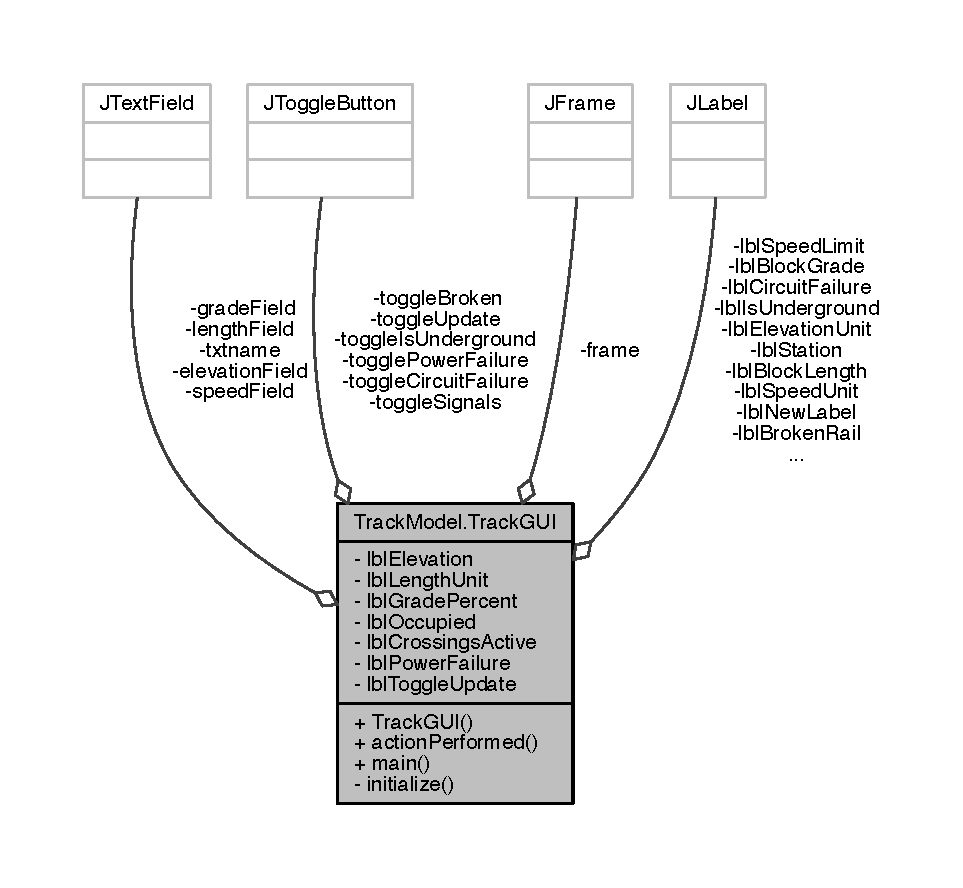
\includegraphics[width=350pt]{classTrackModel_1_1TrackGUI__coll__graph}
\end{center}
\end{figure}
\subsection*{Public Member Functions}
\begin{DoxyCompactItemize}
\item 
\hyperlink{classTrackModel_1_1TrackGUI_a9c9ef6bb307ee64e6eb01f881588f740}{Track\+G\+UI} ()
\begin{DoxyCompactList}\small\item\em Create the application. \end{DoxyCompactList}\item 
void \hyperlink{classTrackModel_1_1TrackGUI_aa7c85f553a7540a8f20b2092d8a6ca8a}{action\+Performed} (Action\+Event e)
\begin{DoxyCompactList}\small\item\em Listens to the combo box and updates the G\+UI based upon the inputs. \end{DoxyCompactList}\end{DoxyCompactItemize}
\subsection*{Static Public Member Functions}
\begin{DoxyCompactItemize}
\item 
static void \hyperlink{classTrackModel_1_1TrackGUI_ae0ea094a8dc49fd550f92a4ad64918d3}{main} (String\mbox{[}$\,$\mbox{]} args)
\begin{DoxyCompactList}\small\item\em Launch the application. \end{DoxyCompactList}\end{DoxyCompactItemize}
\subsection*{Private Member Functions}
\begin{DoxyCompactItemize}
\item 
void \hyperlink{classTrackModel_1_1TrackGUI_a8e4a5b8c6812d1562bd92323025b0f76}{initialize} ()
\begin{DoxyCompactList}\small\item\em Initialize the contents of the frame. \end{DoxyCompactList}\end{DoxyCompactItemize}
\subsection*{Private Attributes}
\begin{DoxyCompactItemize}
\item 
J\+Frame \hyperlink{classTrackModel_1_1TrackGUI_afbf142ba83539e2969d3f71105fcd9bc}{frame}
\item 
J\+Text\+Field \hyperlink{classTrackModel_1_1TrackGUI_ac8d1e32c1ba369deb753a052dd055627}{length\+Field}
\item 
J\+Text\+Field \hyperlink{classTrackModel_1_1TrackGUI_a3f2d40069de0797f2df894ba42df8528}{grade\+Field}
\item 
J\+Text\+Field \hyperlink{classTrackModel_1_1TrackGUI_a4020c45cde27dfcf04a96c1a7136ee33}{elevation\+Field}
\item 
J\+Text\+Field \hyperlink{classTrackModel_1_1TrackGUI_ae38c86c47dd990edffe703acaa29ced0}{speed\+Field}
\item 
J\+Label \hyperlink{classTrackModel_1_1TrackGUI_a0e8f63d8525e33bf35edde9c57a416fd}{lbl\+Block\+Length}
\item 
J\+Label \hyperlink{classTrackModel_1_1TrackGUI_abcc3db1fe345d00632d5a29987eb5f46}{lbl\+Block\+Grade}
\item 
J\+Label \hyperlink{classTrackModel_1_1TrackGUI_a8ea36b1ecc1780cc951415e05069c7fa}{lbl\+Elevation}
\item 
J\+Label \hyperlink{classTrackModel_1_1TrackGUI_a390fd251f4338a570ded42a95ef2d9f8}{lbl\+Speed\+Limit}
\item 
J\+Label \hyperlink{classTrackModel_1_1TrackGUI_ada34f76d9acc01d43aa79033e90855cd}{lbl\+Length\+Unit}
\item 
J\+Label \hyperlink{classTrackModel_1_1TrackGUI_ab42f31f950e3cebdc7b71a9ef35bae6c}{lbl\+Grade\+Percent}
\item 
J\+Label \hyperlink{classTrackModel_1_1TrackGUI_a3140938ab0b72e3984c0787e412d9fee}{lbl\+Elevation\+Unit}
\item 
J\+Label \hyperlink{classTrackModel_1_1TrackGUI_a7238d66f96bc0a85ca437ac6de1faa71}{lbl\+Speed\+Unit}
\item 
J\+Label \hyperlink{classTrackModel_1_1TrackGUI_ac866848253cc9bca3d7a8cbfcf2b5493}{lbl\+Occupied}
\item 
J\+Label \hyperlink{classTrackModel_1_1TrackGUI_a863b8f99c02dac7d8fd51eccf5ddc1f0}{lbl\+Crossings\+Active}
\item 
J\+Label \hyperlink{classTrackModel_1_1TrackGUI_ab1bf4e948e8db5dafdb09ed558140d52}{lbl\+Is\+Underground}
\item 
J\+Toggle\+Button \hyperlink{classTrackModel_1_1TrackGUI_a1fe521ce42539dc1bcbccfb5ed41bbac}{toggle\+Signals}
\item 
J\+Label \hyperlink{classTrackModel_1_1TrackGUI_a7ccc784bfd3fdfde85c4fa8b739f2fcb}{lbl\+Station}
\item 
J\+Text\+Field \hyperlink{classTrackModel_1_1TrackGUI_a86ec145869a52d00f8d983f34bac90f1}{txtname}
\item 
J\+Label \hyperlink{classTrackModel_1_1TrackGUI_a505f3e3b26bcc339146f737a2a85eee5}{lbl\+New\+Label}
\item 
J\+Label \hyperlink{classTrackModel_1_1TrackGUI_a34a858d86011509dfca0ee2a86d36ded}{lbl\+Broken\+Rail}
\item 
J\+Toggle\+Button \hyperlink{classTrackModel_1_1TrackGUI_a3230a1046a2b3b8c66930a0bf8835919}{toggle\+Broken}
\item 
J\+Toggle\+Button \hyperlink{classTrackModel_1_1TrackGUI_a77c0d04ad9154f6a9ce658ec2a4fee75}{toggle\+Circuit\+Failure}
\item 
J\+Label \hyperlink{classTrackModel_1_1TrackGUI_aa11cdf9ec850c3a65799e91707a45f89}{lbl\+Circuit\+Failure}
\item 
J\+Label \hyperlink{classTrackModel_1_1TrackGUI_a1fb949d22e01b87afacfb088b5a2e8cd}{lbl\+Power\+Failure}
\item 
J\+Label \hyperlink{classTrackModel_1_1TrackGUI_a518c15d0e0683b93e65c44bd151a63db}{lbl\+Toggle\+Update}
\item 
J\+Toggle\+Button \hyperlink{classTrackModel_1_1TrackGUI_acf45b0c8d2150d15911a887d4677f7cb}{toggle\+Power\+Failure}
\item 
J\+Toggle\+Button \hyperlink{classTrackModel_1_1TrackGUI_ab6d7083fbc621edf4614fba49425f985}{toggle\+Is\+Underground}
\item 
J\+Toggle\+Button \hyperlink{classTrackModel_1_1TrackGUI_afcc0917c3720c4a4c594aab2a99c868c}{toggle\+Update}
\end{DoxyCompactItemize}


\subsection{Constructor \& Destructor Documentation}
\mbox{\Hypertarget{classTrackModel_1_1TrackGUI_a9c9ef6bb307ee64e6eb01f881588f740}\label{classTrackModel_1_1TrackGUI_a9c9ef6bb307ee64e6eb01f881588f740}} 
\index{Track\+Model\+::\+Track\+G\+UI@{Track\+Model\+::\+Track\+G\+UI}!Track\+G\+UI@{Track\+G\+UI}}
\index{Track\+G\+UI@{Track\+G\+UI}!Track\+Model\+::\+Track\+G\+UI@{Track\+Model\+::\+Track\+G\+UI}}
\subsubsection{\texorpdfstring{Track\+G\+U\+I()}{TrackGUI()}}
{\footnotesize\ttfamily Track\+Model.\+Track\+G\+U\+I.\+Track\+G\+UI (\begin{DoxyParamCaption}{ }\end{DoxyParamCaption})}



Create the application. 



\subsection{Member Function Documentation}
\mbox{\Hypertarget{classTrackModel_1_1TrackGUI_aa7c85f553a7540a8f20b2092d8a6ca8a}\label{classTrackModel_1_1TrackGUI_aa7c85f553a7540a8f20b2092d8a6ca8a}} 
\index{Track\+Model\+::\+Track\+G\+UI@{Track\+Model\+::\+Track\+G\+UI}!action\+Performed@{action\+Performed}}
\index{action\+Performed@{action\+Performed}!Track\+Model\+::\+Track\+G\+UI@{Track\+Model\+::\+Track\+G\+UI}}
\subsubsection{\texorpdfstring{action\+Performed()}{actionPerformed()}}
{\footnotesize\ttfamily void Track\+Model.\+Track\+G\+U\+I.\+action\+Performed (\begin{DoxyParamCaption}\item[{Action\+Event}]{e }\end{DoxyParamCaption})}



Listens to the combo box and updates the G\+UI based upon the inputs. 

\begin{DoxyRefDesc}{Bug}
\item[\hyperlink{bug__bug000001}{Bug}]The segment and block descriptors need to be cleared when selecting a dropdown from line. In its current configuration, it will not reset to empty fields, allowing the user to select blocks that do not exist. This condition applies to selecting a new line while holding segment and block constant.\end{DoxyRefDesc}


\begin{DoxyRefDesc}{Bug}
\item[\hyperlink{bug__bug000002}{Bug}]It is possible for a user to select default vaules in the dropdown menu. When selecting the default values, it results in an unhandled exception, rendering the program unusable. \end{DoxyRefDesc}
\mbox{\Hypertarget{classTrackModel_1_1TrackGUI_a8e4a5b8c6812d1562bd92323025b0f76}\label{classTrackModel_1_1TrackGUI_a8e4a5b8c6812d1562bd92323025b0f76}} 
\index{Track\+Model\+::\+Track\+G\+UI@{Track\+Model\+::\+Track\+G\+UI}!initialize@{initialize}}
\index{initialize@{initialize}!Track\+Model\+::\+Track\+G\+UI@{Track\+Model\+::\+Track\+G\+UI}}
\subsubsection{\texorpdfstring{initialize()}{initialize()}}
{\footnotesize\ttfamily void Track\+Model.\+Track\+G\+U\+I.\+initialize (\begin{DoxyParamCaption}{ }\end{DoxyParamCaption})\hspace{0.3cm}{\ttfamily [private]}}



Initialize the contents of the frame. 

Update button action listeners. Updates the display fields based upon the dropdown buttons selected.\mbox{\Hypertarget{classTrackModel_1_1TrackGUI_ae0ea094a8dc49fd550f92a4ad64918d3}\label{classTrackModel_1_1TrackGUI_ae0ea094a8dc49fd550f92a4ad64918d3}} 
\index{Track\+Model\+::\+Track\+G\+UI@{Track\+Model\+::\+Track\+G\+UI}!main@{main}}
\index{main@{main}!Track\+Model\+::\+Track\+G\+UI@{Track\+Model\+::\+Track\+G\+UI}}
\subsubsection{\texorpdfstring{main()}{main()}}
{\footnotesize\ttfamily static void Track\+Model.\+Track\+G\+U\+I.\+main (\begin{DoxyParamCaption}\item[{String \mbox{[}$\,$\mbox{]}}]{args }\end{DoxyParamCaption})\hspace{0.3cm}{\ttfamily [static]}}



Launch the application. 



\subsection{Member Data Documentation}
\mbox{\Hypertarget{classTrackModel_1_1TrackGUI_a4020c45cde27dfcf04a96c1a7136ee33}\label{classTrackModel_1_1TrackGUI_a4020c45cde27dfcf04a96c1a7136ee33}} 
\index{Track\+Model\+::\+Track\+G\+UI@{Track\+Model\+::\+Track\+G\+UI}!elevation\+Field@{elevation\+Field}}
\index{elevation\+Field@{elevation\+Field}!Track\+Model\+::\+Track\+G\+UI@{Track\+Model\+::\+Track\+G\+UI}}
\subsubsection{\texorpdfstring{elevation\+Field}{elevationField}}
{\footnotesize\ttfamily J\+Text\+Field Track\+Model.\+Track\+G\+U\+I.\+elevation\+Field\hspace{0.3cm}{\ttfamily [private]}}

\mbox{\Hypertarget{classTrackModel_1_1TrackGUI_afbf142ba83539e2969d3f71105fcd9bc}\label{classTrackModel_1_1TrackGUI_afbf142ba83539e2969d3f71105fcd9bc}} 
\index{Track\+Model\+::\+Track\+G\+UI@{Track\+Model\+::\+Track\+G\+UI}!frame@{frame}}
\index{frame@{frame}!Track\+Model\+::\+Track\+G\+UI@{Track\+Model\+::\+Track\+G\+UI}}
\subsubsection{\texorpdfstring{frame}{frame}}
{\footnotesize\ttfamily J\+Frame Track\+Model.\+Track\+G\+U\+I.\+frame\hspace{0.3cm}{\ttfamily [private]}}

\mbox{\Hypertarget{classTrackModel_1_1TrackGUI_a3f2d40069de0797f2df894ba42df8528}\label{classTrackModel_1_1TrackGUI_a3f2d40069de0797f2df894ba42df8528}} 
\index{Track\+Model\+::\+Track\+G\+UI@{Track\+Model\+::\+Track\+G\+UI}!grade\+Field@{grade\+Field}}
\index{grade\+Field@{grade\+Field}!Track\+Model\+::\+Track\+G\+UI@{Track\+Model\+::\+Track\+G\+UI}}
\subsubsection{\texorpdfstring{grade\+Field}{gradeField}}
{\footnotesize\ttfamily J\+Text\+Field Track\+Model.\+Track\+G\+U\+I.\+grade\+Field\hspace{0.3cm}{\ttfamily [private]}}

\mbox{\Hypertarget{classTrackModel_1_1TrackGUI_abcc3db1fe345d00632d5a29987eb5f46}\label{classTrackModel_1_1TrackGUI_abcc3db1fe345d00632d5a29987eb5f46}} 
\index{Track\+Model\+::\+Track\+G\+UI@{Track\+Model\+::\+Track\+G\+UI}!lbl\+Block\+Grade@{lbl\+Block\+Grade}}
\index{lbl\+Block\+Grade@{lbl\+Block\+Grade}!Track\+Model\+::\+Track\+G\+UI@{Track\+Model\+::\+Track\+G\+UI}}
\subsubsection{\texorpdfstring{lbl\+Block\+Grade}{lblBlockGrade}}
{\footnotesize\ttfamily J\+Label Track\+Model.\+Track\+G\+U\+I.\+lbl\+Block\+Grade\hspace{0.3cm}{\ttfamily [private]}}

\mbox{\Hypertarget{classTrackModel_1_1TrackGUI_a0e8f63d8525e33bf35edde9c57a416fd}\label{classTrackModel_1_1TrackGUI_a0e8f63d8525e33bf35edde9c57a416fd}} 
\index{Track\+Model\+::\+Track\+G\+UI@{Track\+Model\+::\+Track\+G\+UI}!lbl\+Block\+Length@{lbl\+Block\+Length}}
\index{lbl\+Block\+Length@{lbl\+Block\+Length}!Track\+Model\+::\+Track\+G\+UI@{Track\+Model\+::\+Track\+G\+UI}}
\subsubsection{\texorpdfstring{lbl\+Block\+Length}{lblBlockLength}}
{\footnotesize\ttfamily J\+Label Track\+Model.\+Track\+G\+U\+I.\+lbl\+Block\+Length\hspace{0.3cm}{\ttfamily [private]}}

\mbox{\Hypertarget{classTrackModel_1_1TrackGUI_a34a858d86011509dfca0ee2a86d36ded}\label{classTrackModel_1_1TrackGUI_a34a858d86011509dfca0ee2a86d36ded}} 
\index{Track\+Model\+::\+Track\+G\+UI@{Track\+Model\+::\+Track\+G\+UI}!lbl\+Broken\+Rail@{lbl\+Broken\+Rail}}
\index{lbl\+Broken\+Rail@{lbl\+Broken\+Rail}!Track\+Model\+::\+Track\+G\+UI@{Track\+Model\+::\+Track\+G\+UI}}
\subsubsection{\texorpdfstring{lbl\+Broken\+Rail}{lblBrokenRail}}
{\footnotesize\ttfamily J\+Label Track\+Model.\+Track\+G\+U\+I.\+lbl\+Broken\+Rail\hspace{0.3cm}{\ttfamily [private]}}

\mbox{\Hypertarget{classTrackModel_1_1TrackGUI_aa11cdf9ec850c3a65799e91707a45f89}\label{classTrackModel_1_1TrackGUI_aa11cdf9ec850c3a65799e91707a45f89}} 
\index{Track\+Model\+::\+Track\+G\+UI@{Track\+Model\+::\+Track\+G\+UI}!lbl\+Circuit\+Failure@{lbl\+Circuit\+Failure}}
\index{lbl\+Circuit\+Failure@{lbl\+Circuit\+Failure}!Track\+Model\+::\+Track\+G\+UI@{Track\+Model\+::\+Track\+G\+UI}}
\subsubsection{\texorpdfstring{lbl\+Circuit\+Failure}{lblCircuitFailure}}
{\footnotesize\ttfamily J\+Label Track\+Model.\+Track\+G\+U\+I.\+lbl\+Circuit\+Failure\hspace{0.3cm}{\ttfamily [private]}}

\mbox{\Hypertarget{classTrackModel_1_1TrackGUI_a863b8f99c02dac7d8fd51eccf5ddc1f0}\label{classTrackModel_1_1TrackGUI_a863b8f99c02dac7d8fd51eccf5ddc1f0}} 
\index{Track\+Model\+::\+Track\+G\+UI@{Track\+Model\+::\+Track\+G\+UI}!lbl\+Crossings\+Active@{lbl\+Crossings\+Active}}
\index{lbl\+Crossings\+Active@{lbl\+Crossings\+Active}!Track\+Model\+::\+Track\+G\+UI@{Track\+Model\+::\+Track\+G\+UI}}
\subsubsection{\texorpdfstring{lbl\+Crossings\+Active}{lblCrossingsActive}}
{\footnotesize\ttfamily J\+Label Track\+Model.\+Track\+G\+U\+I.\+lbl\+Crossings\+Active\hspace{0.3cm}{\ttfamily [private]}}

\mbox{\Hypertarget{classTrackModel_1_1TrackGUI_a8ea36b1ecc1780cc951415e05069c7fa}\label{classTrackModel_1_1TrackGUI_a8ea36b1ecc1780cc951415e05069c7fa}} 
\index{Track\+Model\+::\+Track\+G\+UI@{Track\+Model\+::\+Track\+G\+UI}!lbl\+Elevation@{lbl\+Elevation}}
\index{lbl\+Elevation@{lbl\+Elevation}!Track\+Model\+::\+Track\+G\+UI@{Track\+Model\+::\+Track\+G\+UI}}
\subsubsection{\texorpdfstring{lbl\+Elevation}{lblElevation}}
{\footnotesize\ttfamily J\+Label Track\+Model.\+Track\+G\+U\+I.\+lbl\+Elevation\hspace{0.3cm}{\ttfamily [private]}}

\mbox{\Hypertarget{classTrackModel_1_1TrackGUI_a3140938ab0b72e3984c0787e412d9fee}\label{classTrackModel_1_1TrackGUI_a3140938ab0b72e3984c0787e412d9fee}} 
\index{Track\+Model\+::\+Track\+G\+UI@{Track\+Model\+::\+Track\+G\+UI}!lbl\+Elevation\+Unit@{lbl\+Elevation\+Unit}}
\index{lbl\+Elevation\+Unit@{lbl\+Elevation\+Unit}!Track\+Model\+::\+Track\+G\+UI@{Track\+Model\+::\+Track\+G\+UI}}
\subsubsection{\texorpdfstring{lbl\+Elevation\+Unit}{lblElevationUnit}}
{\footnotesize\ttfamily J\+Label Track\+Model.\+Track\+G\+U\+I.\+lbl\+Elevation\+Unit\hspace{0.3cm}{\ttfamily [private]}}

\mbox{\Hypertarget{classTrackModel_1_1TrackGUI_ab42f31f950e3cebdc7b71a9ef35bae6c}\label{classTrackModel_1_1TrackGUI_ab42f31f950e3cebdc7b71a9ef35bae6c}} 
\index{Track\+Model\+::\+Track\+G\+UI@{Track\+Model\+::\+Track\+G\+UI}!lbl\+Grade\+Percent@{lbl\+Grade\+Percent}}
\index{lbl\+Grade\+Percent@{lbl\+Grade\+Percent}!Track\+Model\+::\+Track\+G\+UI@{Track\+Model\+::\+Track\+G\+UI}}
\subsubsection{\texorpdfstring{lbl\+Grade\+Percent}{lblGradePercent}}
{\footnotesize\ttfamily J\+Label Track\+Model.\+Track\+G\+U\+I.\+lbl\+Grade\+Percent\hspace{0.3cm}{\ttfamily [private]}}

\mbox{\Hypertarget{classTrackModel_1_1TrackGUI_ab1bf4e948e8db5dafdb09ed558140d52}\label{classTrackModel_1_1TrackGUI_ab1bf4e948e8db5dafdb09ed558140d52}} 
\index{Track\+Model\+::\+Track\+G\+UI@{Track\+Model\+::\+Track\+G\+UI}!lbl\+Is\+Underground@{lbl\+Is\+Underground}}
\index{lbl\+Is\+Underground@{lbl\+Is\+Underground}!Track\+Model\+::\+Track\+G\+UI@{Track\+Model\+::\+Track\+G\+UI}}
\subsubsection{\texorpdfstring{lbl\+Is\+Underground}{lblIsUnderground}}
{\footnotesize\ttfamily J\+Label Track\+Model.\+Track\+G\+U\+I.\+lbl\+Is\+Underground\hspace{0.3cm}{\ttfamily [private]}}

\mbox{\Hypertarget{classTrackModel_1_1TrackGUI_ada34f76d9acc01d43aa79033e90855cd}\label{classTrackModel_1_1TrackGUI_ada34f76d9acc01d43aa79033e90855cd}} 
\index{Track\+Model\+::\+Track\+G\+UI@{Track\+Model\+::\+Track\+G\+UI}!lbl\+Length\+Unit@{lbl\+Length\+Unit}}
\index{lbl\+Length\+Unit@{lbl\+Length\+Unit}!Track\+Model\+::\+Track\+G\+UI@{Track\+Model\+::\+Track\+G\+UI}}
\subsubsection{\texorpdfstring{lbl\+Length\+Unit}{lblLengthUnit}}
{\footnotesize\ttfamily J\+Label Track\+Model.\+Track\+G\+U\+I.\+lbl\+Length\+Unit\hspace{0.3cm}{\ttfamily [private]}}

\mbox{\Hypertarget{classTrackModel_1_1TrackGUI_a505f3e3b26bcc339146f737a2a85eee5}\label{classTrackModel_1_1TrackGUI_a505f3e3b26bcc339146f737a2a85eee5}} 
\index{Track\+Model\+::\+Track\+G\+UI@{Track\+Model\+::\+Track\+G\+UI}!lbl\+New\+Label@{lbl\+New\+Label}}
\index{lbl\+New\+Label@{lbl\+New\+Label}!Track\+Model\+::\+Track\+G\+UI@{Track\+Model\+::\+Track\+G\+UI}}
\subsubsection{\texorpdfstring{lbl\+New\+Label}{lblNewLabel}}
{\footnotesize\ttfamily J\+Label Track\+Model.\+Track\+G\+U\+I.\+lbl\+New\+Label\hspace{0.3cm}{\ttfamily [private]}}

\mbox{\Hypertarget{classTrackModel_1_1TrackGUI_ac866848253cc9bca3d7a8cbfcf2b5493}\label{classTrackModel_1_1TrackGUI_ac866848253cc9bca3d7a8cbfcf2b5493}} 
\index{Track\+Model\+::\+Track\+G\+UI@{Track\+Model\+::\+Track\+G\+UI}!lbl\+Occupied@{lbl\+Occupied}}
\index{lbl\+Occupied@{lbl\+Occupied}!Track\+Model\+::\+Track\+G\+UI@{Track\+Model\+::\+Track\+G\+UI}}
\subsubsection{\texorpdfstring{lbl\+Occupied}{lblOccupied}}
{\footnotesize\ttfamily J\+Label Track\+Model.\+Track\+G\+U\+I.\+lbl\+Occupied\hspace{0.3cm}{\ttfamily [private]}}

\mbox{\Hypertarget{classTrackModel_1_1TrackGUI_a1fb949d22e01b87afacfb088b5a2e8cd}\label{classTrackModel_1_1TrackGUI_a1fb949d22e01b87afacfb088b5a2e8cd}} 
\index{Track\+Model\+::\+Track\+G\+UI@{Track\+Model\+::\+Track\+G\+UI}!lbl\+Power\+Failure@{lbl\+Power\+Failure}}
\index{lbl\+Power\+Failure@{lbl\+Power\+Failure}!Track\+Model\+::\+Track\+G\+UI@{Track\+Model\+::\+Track\+G\+UI}}
\subsubsection{\texorpdfstring{lbl\+Power\+Failure}{lblPowerFailure}}
{\footnotesize\ttfamily J\+Label Track\+Model.\+Track\+G\+U\+I.\+lbl\+Power\+Failure\hspace{0.3cm}{\ttfamily [private]}}

\mbox{\Hypertarget{classTrackModel_1_1TrackGUI_a390fd251f4338a570ded42a95ef2d9f8}\label{classTrackModel_1_1TrackGUI_a390fd251f4338a570ded42a95ef2d9f8}} 
\index{Track\+Model\+::\+Track\+G\+UI@{Track\+Model\+::\+Track\+G\+UI}!lbl\+Speed\+Limit@{lbl\+Speed\+Limit}}
\index{lbl\+Speed\+Limit@{lbl\+Speed\+Limit}!Track\+Model\+::\+Track\+G\+UI@{Track\+Model\+::\+Track\+G\+UI}}
\subsubsection{\texorpdfstring{lbl\+Speed\+Limit}{lblSpeedLimit}}
{\footnotesize\ttfamily J\+Label Track\+Model.\+Track\+G\+U\+I.\+lbl\+Speed\+Limit\hspace{0.3cm}{\ttfamily [private]}}

\mbox{\Hypertarget{classTrackModel_1_1TrackGUI_a7238d66f96bc0a85ca437ac6de1faa71}\label{classTrackModel_1_1TrackGUI_a7238d66f96bc0a85ca437ac6de1faa71}} 
\index{Track\+Model\+::\+Track\+G\+UI@{Track\+Model\+::\+Track\+G\+UI}!lbl\+Speed\+Unit@{lbl\+Speed\+Unit}}
\index{lbl\+Speed\+Unit@{lbl\+Speed\+Unit}!Track\+Model\+::\+Track\+G\+UI@{Track\+Model\+::\+Track\+G\+UI}}
\subsubsection{\texorpdfstring{lbl\+Speed\+Unit}{lblSpeedUnit}}
{\footnotesize\ttfamily J\+Label Track\+Model.\+Track\+G\+U\+I.\+lbl\+Speed\+Unit\hspace{0.3cm}{\ttfamily [private]}}

\mbox{\Hypertarget{classTrackModel_1_1TrackGUI_a7ccc784bfd3fdfde85c4fa8b739f2fcb}\label{classTrackModel_1_1TrackGUI_a7ccc784bfd3fdfde85c4fa8b739f2fcb}} 
\index{Track\+Model\+::\+Track\+G\+UI@{Track\+Model\+::\+Track\+G\+UI}!lbl\+Station@{lbl\+Station}}
\index{lbl\+Station@{lbl\+Station}!Track\+Model\+::\+Track\+G\+UI@{Track\+Model\+::\+Track\+G\+UI}}
\subsubsection{\texorpdfstring{lbl\+Station}{lblStation}}
{\footnotesize\ttfamily J\+Label Track\+Model.\+Track\+G\+U\+I.\+lbl\+Station\hspace{0.3cm}{\ttfamily [private]}}

\mbox{\Hypertarget{classTrackModel_1_1TrackGUI_a518c15d0e0683b93e65c44bd151a63db}\label{classTrackModel_1_1TrackGUI_a518c15d0e0683b93e65c44bd151a63db}} 
\index{Track\+Model\+::\+Track\+G\+UI@{Track\+Model\+::\+Track\+G\+UI}!lbl\+Toggle\+Update@{lbl\+Toggle\+Update}}
\index{lbl\+Toggle\+Update@{lbl\+Toggle\+Update}!Track\+Model\+::\+Track\+G\+UI@{Track\+Model\+::\+Track\+G\+UI}}
\subsubsection{\texorpdfstring{lbl\+Toggle\+Update}{lblToggleUpdate}}
{\footnotesize\ttfamily J\+Label Track\+Model.\+Track\+G\+U\+I.\+lbl\+Toggle\+Update\hspace{0.3cm}{\ttfamily [private]}}

\mbox{\Hypertarget{classTrackModel_1_1TrackGUI_ac8d1e32c1ba369deb753a052dd055627}\label{classTrackModel_1_1TrackGUI_ac8d1e32c1ba369deb753a052dd055627}} 
\index{Track\+Model\+::\+Track\+G\+UI@{Track\+Model\+::\+Track\+G\+UI}!length\+Field@{length\+Field}}
\index{length\+Field@{length\+Field}!Track\+Model\+::\+Track\+G\+UI@{Track\+Model\+::\+Track\+G\+UI}}
\subsubsection{\texorpdfstring{length\+Field}{lengthField}}
{\footnotesize\ttfamily J\+Text\+Field Track\+Model.\+Track\+G\+U\+I.\+length\+Field\hspace{0.3cm}{\ttfamily [private]}}

\mbox{\Hypertarget{classTrackModel_1_1TrackGUI_ae38c86c47dd990edffe703acaa29ced0}\label{classTrackModel_1_1TrackGUI_ae38c86c47dd990edffe703acaa29ced0}} 
\index{Track\+Model\+::\+Track\+G\+UI@{Track\+Model\+::\+Track\+G\+UI}!speed\+Field@{speed\+Field}}
\index{speed\+Field@{speed\+Field}!Track\+Model\+::\+Track\+G\+UI@{Track\+Model\+::\+Track\+G\+UI}}
\subsubsection{\texorpdfstring{speed\+Field}{speedField}}
{\footnotesize\ttfamily J\+Text\+Field Track\+Model.\+Track\+G\+U\+I.\+speed\+Field\hspace{0.3cm}{\ttfamily [private]}}

\mbox{\Hypertarget{classTrackModel_1_1TrackGUI_a3230a1046a2b3b8c66930a0bf8835919}\label{classTrackModel_1_1TrackGUI_a3230a1046a2b3b8c66930a0bf8835919}} 
\index{Track\+Model\+::\+Track\+G\+UI@{Track\+Model\+::\+Track\+G\+UI}!toggle\+Broken@{toggle\+Broken}}
\index{toggle\+Broken@{toggle\+Broken}!Track\+Model\+::\+Track\+G\+UI@{Track\+Model\+::\+Track\+G\+UI}}
\subsubsection{\texorpdfstring{toggle\+Broken}{toggleBroken}}
{\footnotesize\ttfamily J\+Toggle\+Button Track\+Model.\+Track\+G\+U\+I.\+toggle\+Broken\hspace{0.3cm}{\ttfamily [private]}}

\mbox{\Hypertarget{classTrackModel_1_1TrackGUI_a77c0d04ad9154f6a9ce658ec2a4fee75}\label{classTrackModel_1_1TrackGUI_a77c0d04ad9154f6a9ce658ec2a4fee75}} 
\index{Track\+Model\+::\+Track\+G\+UI@{Track\+Model\+::\+Track\+G\+UI}!toggle\+Circuit\+Failure@{toggle\+Circuit\+Failure}}
\index{toggle\+Circuit\+Failure@{toggle\+Circuit\+Failure}!Track\+Model\+::\+Track\+G\+UI@{Track\+Model\+::\+Track\+G\+UI}}
\subsubsection{\texorpdfstring{toggle\+Circuit\+Failure}{toggleCircuitFailure}}
{\footnotesize\ttfamily J\+Toggle\+Button Track\+Model.\+Track\+G\+U\+I.\+toggle\+Circuit\+Failure\hspace{0.3cm}{\ttfamily [private]}}

\mbox{\Hypertarget{classTrackModel_1_1TrackGUI_ab6d7083fbc621edf4614fba49425f985}\label{classTrackModel_1_1TrackGUI_ab6d7083fbc621edf4614fba49425f985}} 
\index{Track\+Model\+::\+Track\+G\+UI@{Track\+Model\+::\+Track\+G\+UI}!toggle\+Is\+Underground@{toggle\+Is\+Underground}}
\index{toggle\+Is\+Underground@{toggle\+Is\+Underground}!Track\+Model\+::\+Track\+G\+UI@{Track\+Model\+::\+Track\+G\+UI}}
\subsubsection{\texorpdfstring{toggle\+Is\+Underground}{toggleIsUnderground}}
{\footnotesize\ttfamily J\+Toggle\+Button Track\+Model.\+Track\+G\+U\+I.\+toggle\+Is\+Underground\hspace{0.3cm}{\ttfamily [private]}}

\mbox{\Hypertarget{classTrackModel_1_1TrackGUI_acf45b0c8d2150d15911a887d4677f7cb}\label{classTrackModel_1_1TrackGUI_acf45b0c8d2150d15911a887d4677f7cb}} 
\index{Track\+Model\+::\+Track\+G\+UI@{Track\+Model\+::\+Track\+G\+UI}!toggle\+Power\+Failure@{toggle\+Power\+Failure}}
\index{toggle\+Power\+Failure@{toggle\+Power\+Failure}!Track\+Model\+::\+Track\+G\+UI@{Track\+Model\+::\+Track\+G\+UI}}
\subsubsection{\texorpdfstring{toggle\+Power\+Failure}{togglePowerFailure}}
{\footnotesize\ttfamily J\+Toggle\+Button Track\+Model.\+Track\+G\+U\+I.\+toggle\+Power\+Failure\hspace{0.3cm}{\ttfamily [private]}}

\mbox{\Hypertarget{classTrackModel_1_1TrackGUI_a1fe521ce42539dc1bcbccfb5ed41bbac}\label{classTrackModel_1_1TrackGUI_a1fe521ce42539dc1bcbccfb5ed41bbac}} 
\index{Track\+Model\+::\+Track\+G\+UI@{Track\+Model\+::\+Track\+G\+UI}!toggle\+Signals@{toggle\+Signals}}
\index{toggle\+Signals@{toggle\+Signals}!Track\+Model\+::\+Track\+G\+UI@{Track\+Model\+::\+Track\+G\+UI}}
\subsubsection{\texorpdfstring{toggle\+Signals}{toggleSignals}}
{\footnotesize\ttfamily J\+Toggle\+Button Track\+Model.\+Track\+G\+U\+I.\+toggle\+Signals\hspace{0.3cm}{\ttfamily [private]}}

\mbox{\Hypertarget{classTrackModel_1_1TrackGUI_afcc0917c3720c4a4c594aab2a99c868c}\label{classTrackModel_1_1TrackGUI_afcc0917c3720c4a4c594aab2a99c868c}} 
\index{Track\+Model\+::\+Track\+G\+UI@{Track\+Model\+::\+Track\+G\+UI}!toggle\+Update@{toggle\+Update}}
\index{toggle\+Update@{toggle\+Update}!Track\+Model\+::\+Track\+G\+UI@{Track\+Model\+::\+Track\+G\+UI}}
\subsubsection{\texorpdfstring{toggle\+Update}{toggleUpdate}}
{\footnotesize\ttfamily J\+Toggle\+Button Track\+Model.\+Track\+G\+U\+I.\+toggle\+Update\hspace{0.3cm}{\ttfamily [private]}}

\mbox{\Hypertarget{classTrackModel_1_1TrackGUI_a86ec145869a52d00f8d983f34bac90f1}\label{classTrackModel_1_1TrackGUI_a86ec145869a52d00f8d983f34bac90f1}} 
\index{Track\+Model\+::\+Track\+G\+UI@{Track\+Model\+::\+Track\+G\+UI}!txtname@{txtname}}
\index{txtname@{txtname}!Track\+Model\+::\+Track\+G\+UI@{Track\+Model\+::\+Track\+G\+UI}}
\subsubsection{\texorpdfstring{txtname}{txtname}}
{\footnotesize\ttfamily J\+Text\+Field Track\+Model.\+Track\+G\+U\+I.\+txtname\hspace{0.3cm}{\ttfamily [private]}}



The documentation for this class was generated from the following file\+:\begin{DoxyCompactItemize}
\item 
src/main/java/\+Track\+Model/\hyperlink{TrackGUI_8java}{Track\+G\+U\+I.\+java}\end{DoxyCompactItemize}

\hypertarget{classTrackModel_1_1TrackModel}{}\section{Track\+Model.\+Track\+Model Class Reference}
\label{classTrackModel_1_1TrackModel}\index{Track\+Model.\+Track\+Model@{Track\+Model.\+Track\+Model}}


Collaboration diagram for Track\+Model.\+Track\+Model\+:
\nopagebreak
\begin{figure}[H]
\begin{center}
\leavevmode
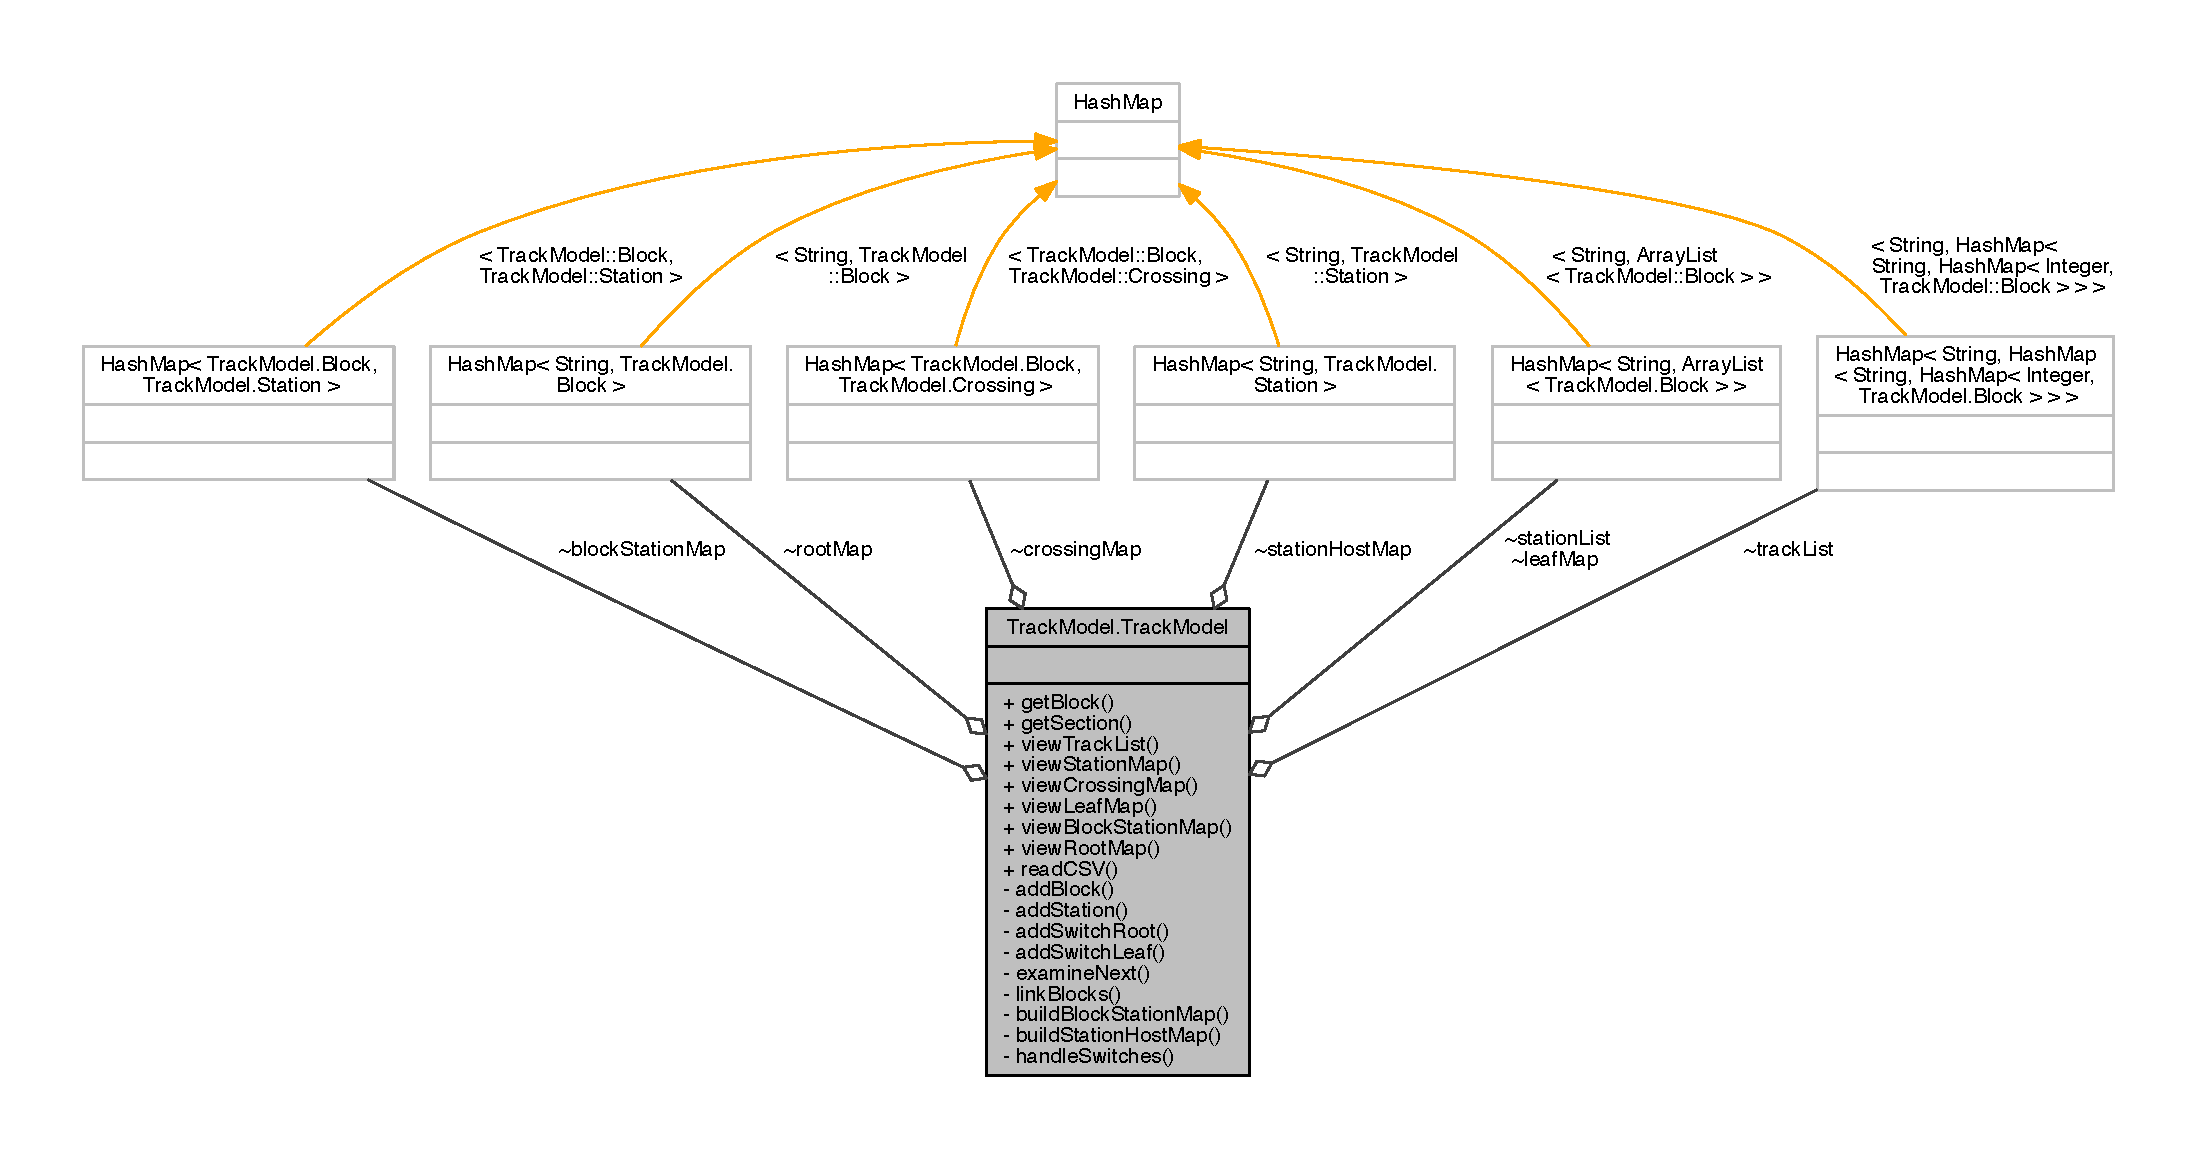
\includegraphics[width=350pt]{classTrackModel_1_1TrackModel__coll__graph}
\end{center}
\end{figure}
\subsection*{Public Member Functions}
\begin{DoxyCompactItemize}
\item 
\hyperlink{classTrackModel_1_1Block}{Block} \hyperlink{classTrackModel_1_1TrackModel_a670006658bfbfc272c1097de1080d17c}{get\+Block} (String line, String section, Integer block\+Num)
\begin{DoxyCompactList}\small\item\em Simplicity wrapper to return a non-\/aliased block on the track given the parameters. \end{DoxyCompactList}\item 
Hash\+Map$<$ Integer, \hyperlink{classTrackModel_1_1Block}{Block} $>$ \hyperlink{classTrackModel_1_1TrackModel_a19d3841da17500d43607ce4f37fc2de9}{get\+Section} (String line, String section)
\begin{DoxyCompactList}\small\item\em Returns a non-\/aliased section of blocks. \end{DoxyCompactList}\item 
Hash\+Map$<$ String, Hash\+Map$<$ String, Hash\+Map$<$ Integer, \hyperlink{classTrackModel_1_1Block}{Block} $>$ $>$ $>$ \hyperlink{classTrackModel_1_1TrackModel_ae74a6b0938494affe4c2b96b7b8f288a}{view\+Track\+List} ()
\begin{DoxyCompactList}\small\item\em Allows viewing of the track\+List to other modules, implemented as a copy method. \end{DoxyCompactList}\item 
Hash\+Map$<$ String, Array\+List$<$ \hyperlink{classTrackModel_1_1Block}{Block} $>$ $>$ \hyperlink{classTrackModel_1_1TrackModel_ae43164d0e8478c2bc5ffc3b013f49e60}{view\+Station\+Map} ()
\begin{DoxyCompactList}\small\item\em Allows viewing of the station map to other modules, implemented as a copy method. \end{DoxyCompactList}\item 
Hash\+Map$<$ \hyperlink{classTrackModel_1_1Block}{Block}, \hyperlink{classTrackModel_1_1Crossing}{Crossing} $>$ \hyperlink{classTrackModel_1_1TrackModel_a5f9d06be603a4aee4d29da60276b0383}{view\+Crossing\+Map} ()
\item 
Hash\+Map$<$ String, Array\+List$<$ \hyperlink{classTrackModel_1_1Block}{Block} $>$ $>$ \hyperlink{classTrackModel_1_1TrackModel_a03ca2c29d73dd39a2dfb3e0342fe4e27}{view\+Leaf\+Map} ()
\begin{DoxyCompactList}\small\item\em Allows viewing of leaf nodes of the switches to other modules. \end{DoxyCompactList}\item 
Hash\+Map$<$ \hyperlink{classTrackModel_1_1Block}{Block}, \hyperlink{classTrackModel_1_1Station}{Station} $>$ \hyperlink{classTrackModel_1_1TrackModel_a5bd341c8df3e0ad585f32e1587061f36}{view\+Block\+Station\+Map} ()
\begin{DoxyCompactList}\small\item\em Allows viewing of the block\+Station\+Map by other modules. \end{DoxyCompactList}\item 
Hash\+Map$<$ String, \hyperlink{classTrackModel_1_1Block}{Block} $>$ \hyperlink{classTrackModel_1_1TrackModel_aa070a8864c352ab49eae4c93aa88700f}{view\+Root\+Map} ()
\begin{DoxyCompactList}\small\item\em Allows viewing of the root\+Map by other modules. \end{DoxyCompactList}\item 
void \hyperlink{classTrackModel_1_1TrackModel_ab4deefd42535c2e06785eba4ed3989a1}{read\+C\+SV} (String\mbox{[}$\,$\mbox{]} f\+Names)
\begin{DoxyCompactList}\small\item\em Helper function for reading the information from the excel-\/dumped C\+SV. \end{DoxyCompactList}\end{DoxyCompactItemize}
\subsection*{Package Attributes}
\begin{DoxyCompactItemize}
\item 
Hash\+Map$<$ String, Hash\+Map$<$ String, Hash\+Map$<$ Integer, \hyperlink{classTrackModel_1_1Block}{Block} $>$ $>$ $>$ \hyperlink{classTrackModel_1_1TrackModel_ad9f221dc431ebf142e7930d8116cf705}{track\+List}
\item 
Hash\+Map$<$ String, \hyperlink{classTrackModel_1_1Block}{Block} $>$ \hyperlink{classTrackModel_1_1TrackModel_ae48e24ae7b5775111086a3b3734d8dc9}{root\+Map} = new Hash\+Map$<$String, \hyperlink{classTrackModel_1_1Block}{Block}$>$()
\item 
Hash\+Map$<$ String, Array\+List$<$ \hyperlink{classTrackModel_1_1Block}{Block} $>$ $>$ \hyperlink{classTrackModel_1_1TrackModel_aaba2349b7ccd094c05ad27c241143e4c}{leaf\+Map} = new Hash\+Map$<$String, Array\+List$<$\hyperlink{classTrackModel_1_1Block}{Block}$>$$>$()
\item 
Hash\+Map$<$ String, Array\+List$<$ \hyperlink{classTrackModel_1_1Block}{Block} $>$ $>$ \hyperlink{classTrackModel_1_1TrackModel_a83c47537abca60251a9b99454db44b28}{station\+List} = new Hash\+Map$<$String, Array\+List$<$\hyperlink{classTrackModel_1_1Block}{Block}$>$$>$()
\item 
Hash\+Map$<$ String, \hyperlink{classTrackModel_1_1Station}{Station} $>$ \hyperlink{classTrackModel_1_1TrackModel_ac81567431e40365448d71a3411711569}{station\+Host\+Map} = new Hash\+Map$<$String, \hyperlink{classTrackModel_1_1Station}{Station}$>$()
\item 
Hash\+Map$<$ \hyperlink{classTrackModel_1_1Block}{Block}, \hyperlink{classTrackModel_1_1Station}{Station} $>$ \hyperlink{classTrackModel_1_1TrackModel_aad5a0edef2a616a3db51d6c5d249c896}{block\+Station\+Map} = new Hash\+Map$<$\hyperlink{classTrackModel_1_1Block}{Block}, \hyperlink{classTrackModel_1_1Station}{Station}$>$()
\item 
Hash\+Map$<$ \hyperlink{classTrackModel_1_1Block}{Block}, \hyperlink{classTrackModel_1_1Crossing}{Crossing} $>$ \hyperlink{classTrackModel_1_1TrackModel_a3615fcccbc32c0bc531e67e9fcd8f51e}{crossing\+Map} = new Hash\+Map$<$\hyperlink{classTrackModel_1_1Block}{Block}, \hyperlink{classTrackModel_1_1Crossing}{Crossing}$>$()
\end{DoxyCompactItemize}
\subsection*{Private Member Functions}
\begin{DoxyCompactItemize}
\item 
void \hyperlink{classTrackModel_1_1TrackModel_aeeec35a2eb38afc82b87fd310f161e9e}{add\+Block} (\hyperlink{classTrackModel_1_1Block}{Block} block)
\begin{DoxyCompactList}\small\item\em Adds a selected block to the \hyperlink{classTrackModel_1_1TrackModel}{Track\+Model}. \end{DoxyCompactList}\item 
void \hyperlink{classTrackModel_1_1TrackModel_a4c6034df7cc2dc75d516b49b2836d30b}{add\+Station} (String station\+Name, \hyperlink{classTrackModel_1_1Block}{Block} station\+Location)
\begin{DoxyCompactList}\small\item\em Adds a station-\/block pair to the station\+List. \end{DoxyCompactList}\item 
void \hyperlink{classTrackModel_1_1TrackModel_ab7bbc240d2612ca3709889f75cf1d40e}{add\+Switch\+Root} (String root\+Block\+String, \hyperlink{classTrackModel_1_1Block}{Block} root\+Block)
\begin{DoxyCompactList}\small\item\em Adds a switch to the root list of the switches present on a given line. \end{DoxyCompactList}\item 
void \hyperlink{classTrackModel_1_1TrackModel_acf1825e32611df62702740caddbb3698}{add\+Switch\+Leaf} (String leaf\+Block\+String, \hyperlink{classTrackModel_1_1Block}{Block} leaf\+Block)
\item 
void \hyperlink{classTrackModel_1_1TrackModel_a70726fc21e809d98f488fe5b80db7631}{examine\+Next} ()
\begin{DoxyCompactList}\small\item\em A small function to view the next and previous blocks of a track model. \end{DoxyCompactList}\item 
void \hyperlink{classTrackModel_1_1TrackModel_a8a320bcb2c2272eb52e05a022f6d4a9c}{link\+Blocks} ()
\begin{DoxyCompactList}\small\item\em Links blocks across block and sections. \end{DoxyCompactList}\item 
void \hyperlink{classTrackModel_1_1TrackModel_a09958c9377126378d1efe5054e246405}{build\+Block\+Station\+Map} ()
\begin{DoxyCompactList}\small\item\em Build a map for storing the blocks and station for use by the train controller and train model. \end{DoxyCompactList}\item 
void \hyperlink{classTrackModel_1_1TrackModel_a6956005761fa4dbe6272088f5f2a2718}{build\+Station\+Host\+Map} ()
\begin{DoxyCompactList}\small\item\em Build the listing of the host station list for external consumption. \end{DoxyCompactList}\item 
void \hyperlink{classTrackModel_1_1TrackModel_a468c19408a6939f20fa6e66b20f8e8ac}{handle\+Switches} ()
\begin{DoxyCompactList}\small\item\em Helper function to link next\+Block for switches. \end{DoxyCompactList}\end{DoxyCompactItemize}


\subsection{Member Function Documentation}
\mbox{\Hypertarget{classTrackModel_1_1TrackModel_aeeec35a2eb38afc82b87fd310f161e9e}\label{classTrackModel_1_1TrackModel_aeeec35a2eb38afc82b87fd310f161e9e}} 
\index{Track\+Model\+::\+Track\+Model@{Track\+Model\+::\+Track\+Model}!add\+Block@{add\+Block}}
\index{add\+Block@{add\+Block}!Track\+Model\+::\+Track\+Model@{Track\+Model\+::\+Track\+Model}}
\subsubsection{\texorpdfstring{add\+Block()}{addBlock()}}
{\footnotesize\ttfamily void Track\+Model.\+Track\+Model.\+add\+Block (\begin{DoxyParamCaption}\item[{\hyperlink{classTrackModel_1_1Block}{Block}}]{block }\end{DoxyParamCaption})\hspace{0.3cm}{\ttfamily [private]}}



Adds a selected block to the \hyperlink{classTrackModel_1_1TrackModel}{Track\+Model}. 

Expects a valid \hyperlink{classTrackModel_1_1Block}{Block} object.


\begin{DoxyParams}{Parameters}
{\em block} & The block to be added. \\
\hline
\end{DoxyParams}
\mbox{\Hypertarget{classTrackModel_1_1TrackModel_a4c6034df7cc2dc75d516b49b2836d30b}\label{classTrackModel_1_1TrackModel_a4c6034df7cc2dc75d516b49b2836d30b}} 
\index{Track\+Model\+::\+Track\+Model@{Track\+Model\+::\+Track\+Model}!add\+Station@{add\+Station}}
\index{add\+Station@{add\+Station}!Track\+Model\+::\+Track\+Model@{Track\+Model\+::\+Track\+Model}}
\subsubsection{\texorpdfstring{add\+Station()}{addStation()}}
{\footnotesize\ttfamily void Track\+Model.\+Track\+Model.\+add\+Station (\begin{DoxyParamCaption}\item[{String}]{station\+Name,  }\item[{\hyperlink{classTrackModel_1_1Block}{Block}}]{station\+Location }\end{DoxyParamCaption})\hspace{0.3cm}{\ttfamily [private]}}



Adds a station-\/block pair to the station\+List. 


\begin{DoxyParams}{Parameters}
{\em station\+Name} & station to be added to the station\+List \\
\hline
{\em station\+Location} & the block location of an point where the station interacts with the block \\
\hline
\end{DoxyParams}
\mbox{\Hypertarget{classTrackModel_1_1TrackModel_acf1825e32611df62702740caddbb3698}\label{classTrackModel_1_1TrackModel_acf1825e32611df62702740caddbb3698}} 
\index{Track\+Model\+::\+Track\+Model@{Track\+Model\+::\+Track\+Model}!add\+Switch\+Leaf@{add\+Switch\+Leaf}}
\index{add\+Switch\+Leaf@{add\+Switch\+Leaf}!Track\+Model\+::\+Track\+Model@{Track\+Model\+::\+Track\+Model}}
\subsubsection{\texorpdfstring{add\+Switch\+Leaf()}{addSwitchLeaf()}}
{\footnotesize\ttfamily void Track\+Model.\+Track\+Model.\+add\+Switch\+Leaf (\begin{DoxyParamCaption}\item[{String}]{leaf\+Block\+String,  }\item[{\hyperlink{classTrackModel_1_1Block}{Block}}]{leaf\+Block }\end{DoxyParamCaption})\hspace{0.3cm}{\ttfamily [private]}}

\mbox{\Hypertarget{classTrackModel_1_1TrackModel_ab7bbc240d2612ca3709889f75cf1d40e}\label{classTrackModel_1_1TrackModel_ab7bbc240d2612ca3709889f75cf1d40e}} 
\index{Track\+Model\+::\+Track\+Model@{Track\+Model\+::\+Track\+Model}!add\+Switch\+Root@{add\+Switch\+Root}}
\index{add\+Switch\+Root@{add\+Switch\+Root}!Track\+Model\+::\+Track\+Model@{Track\+Model\+::\+Track\+Model}}
\subsubsection{\texorpdfstring{add\+Switch\+Root()}{addSwitchRoot()}}
{\footnotesize\ttfamily void Track\+Model.\+Track\+Model.\+add\+Switch\+Root (\begin{DoxyParamCaption}\item[{String}]{root\+Block\+String,  }\item[{\hyperlink{classTrackModel_1_1Block}{Block}}]{root\+Block }\end{DoxyParamCaption})\hspace{0.3cm}{\ttfamily [private]}}



Adds a switch to the root list of the switches present on a given line. 


\begin{DoxyParams}{Parameters}
{\em root\+Block\+String} & String of the added switch to be added to as the \char`\"{}root\char`\"{} switch \\
\hline
{\em root\+Block} & The block where that will point between two blocks depending on the current state of the switch \\
\hline
\end{DoxyParams}
\mbox{\Hypertarget{classTrackModel_1_1TrackModel_a09958c9377126378d1efe5054e246405}\label{classTrackModel_1_1TrackModel_a09958c9377126378d1efe5054e246405}} 
\index{Track\+Model\+::\+Track\+Model@{Track\+Model\+::\+Track\+Model}!build\+Block\+Station\+Map@{build\+Block\+Station\+Map}}
\index{build\+Block\+Station\+Map@{build\+Block\+Station\+Map}!Track\+Model\+::\+Track\+Model@{Track\+Model\+::\+Track\+Model}}
\subsubsection{\texorpdfstring{build\+Block\+Station\+Map()}{buildBlockStationMap()}}
{\footnotesize\ttfamily void Track\+Model.\+Track\+Model.\+build\+Block\+Station\+Map (\begin{DoxyParamCaption}{ }\end{DoxyParamCaption})\hspace{0.3cm}{\ttfamily [private]}}



Build a map for storing the blocks and station for use by the train controller and train model. 

\mbox{\Hypertarget{classTrackModel_1_1TrackModel_a6956005761fa4dbe6272088f5f2a2718}\label{classTrackModel_1_1TrackModel_a6956005761fa4dbe6272088f5f2a2718}} 
\index{Track\+Model\+::\+Track\+Model@{Track\+Model\+::\+Track\+Model}!build\+Station\+Host\+Map@{build\+Station\+Host\+Map}}
\index{build\+Station\+Host\+Map@{build\+Station\+Host\+Map}!Track\+Model\+::\+Track\+Model@{Track\+Model\+::\+Track\+Model}}
\subsubsection{\texorpdfstring{build\+Station\+Host\+Map()}{buildStationHostMap()}}
{\footnotesize\ttfamily void Track\+Model.\+Track\+Model.\+build\+Station\+Host\+Map (\begin{DoxyParamCaption}{ }\end{DoxyParamCaption})\hspace{0.3cm}{\ttfamily [private]}}



Build the listing of the host station list for external consumption. 

\mbox{\Hypertarget{classTrackModel_1_1TrackModel_a70726fc21e809d98f488fe5b80db7631}\label{classTrackModel_1_1TrackModel_a70726fc21e809d98f488fe5b80db7631}} 
\index{Track\+Model\+::\+Track\+Model@{Track\+Model\+::\+Track\+Model}!examine\+Next@{examine\+Next}}
\index{examine\+Next@{examine\+Next}!Track\+Model\+::\+Track\+Model@{Track\+Model\+::\+Track\+Model}}
\subsubsection{\texorpdfstring{examine\+Next()}{examineNext()}}
{\footnotesize\ttfamily void Track\+Model.\+Track\+Model.\+examine\+Next (\begin{DoxyParamCaption}{ }\end{DoxyParamCaption})\hspace{0.3cm}{\ttfamily [private]}}



A small function to view the next and previous blocks of a track model. 

\mbox{\Hypertarget{classTrackModel_1_1TrackModel_a670006658bfbfc272c1097de1080d17c}\label{classTrackModel_1_1TrackModel_a670006658bfbfc272c1097de1080d17c}} 
\index{Track\+Model\+::\+Track\+Model@{Track\+Model\+::\+Track\+Model}!get\+Block@{get\+Block}}
\index{get\+Block@{get\+Block}!Track\+Model\+::\+Track\+Model@{Track\+Model\+::\+Track\+Model}}
\subsubsection{\texorpdfstring{get\+Block()}{getBlock()}}
{\footnotesize\ttfamily \hyperlink{classTrackModel_1_1Block}{Block} Track\+Model.\+Track\+Model.\+get\+Block (\begin{DoxyParamCaption}\item[{String}]{line,  }\item[{String}]{section,  }\item[{Integer}]{block\+Num }\end{DoxyParamCaption})}



Simplicity wrapper to return a non-\/aliased block on the track given the parameters. 


\begin{DoxyParams}{Parameters}
{\em line} & Line of the block to be looked up \\
\hline
{\em section} & Section of the block to be looked up \\
\hline
{\em block\+Num} & Number of the block to be looked up \\
\hline
\end{DoxyParams}
\mbox{\Hypertarget{classTrackModel_1_1TrackModel_a19d3841da17500d43607ce4f37fc2de9}\label{classTrackModel_1_1TrackModel_a19d3841da17500d43607ce4f37fc2de9}} 
\index{Track\+Model\+::\+Track\+Model@{Track\+Model\+::\+Track\+Model}!get\+Section@{get\+Section}}
\index{get\+Section@{get\+Section}!Track\+Model\+::\+Track\+Model@{Track\+Model\+::\+Track\+Model}}
\subsubsection{\texorpdfstring{get\+Section()}{getSection()}}
{\footnotesize\ttfamily Hash\+Map$<$Integer, \hyperlink{classTrackModel_1_1Block}{Block}$>$ Track\+Model.\+Track\+Model.\+get\+Section (\begin{DoxyParamCaption}\item[{String}]{line,  }\item[{String}]{section }\end{DoxyParamCaption})}



Returns a non-\/aliased section of blocks. 


\begin{DoxyParams}{Parameters}
{\em line} & line the section is on \\
\hline
{\em section} & section being requested \\
\hline
\end{DoxyParams}
\mbox{\Hypertarget{classTrackModel_1_1TrackModel_a468c19408a6939f20fa6e66b20f8e8ac}\label{classTrackModel_1_1TrackModel_a468c19408a6939f20fa6e66b20f8e8ac}} 
\index{Track\+Model\+::\+Track\+Model@{Track\+Model\+::\+Track\+Model}!handle\+Switches@{handle\+Switches}}
\index{handle\+Switches@{handle\+Switches}!Track\+Model\+::\+Track\+Model@{Track\+Model\+::\+Track\+Model}}
\subsubsection{\texorpdfstring{handle\+Switches()}{handleSwitches()}}
{\footnotesize\ttfamily void Track\+Model.\+Track\+Model.\+handle\+Switches (\begin{DoxyParamCaption}{ }\end{DoxyParamCaption})\hspace{0.3cm}{\ttfamily [private]}}



Helper function to link next\+Block for switches. 

\mbox{\Hypertarget{classTrackModel_1_1TrackModel_a8a320bcb2c2272eb52e05a022f6d4a9c}\label{classTrackModel_1_1TrackModel_a8a320bcb2c2272eb52e05a022f6d4a9c}} 
\index{Track\+Model\+::\+Track\+Model@{Track\+Model\+::\+Track\+Model}!link\+Blocks@{link\+Blocks}}
\index{link\+Blocks@{link\+Blocks}!Track\+Model\+::\+Track\+Model@{Track\+Model\+::\+Track\+Model}}
\subsubsection{\texorpdfstring{link\+Blocks()}{linkBlocks()}}
{\footnotesize\ttfamily void Track\+Model.\+Track\+Model.\+link\+Blocks (\begin{DoxyParamCaption}{ }\end{DoxyParamCaption})\hspace{0.3cm}{\ttfamily [private]}}



Links blocks across block and sections. 

\mbox{\Hypertarget{classTrackModel_1_1TrackModel_ab4deefd42535c2e06785eba4ed3989a1}\label{classTrackModel_1_1TrackModel_ab4deefd42535c2e06785eba4ed3989a1}} 
\index{Track\+Model\+::\+Track\+Model@{Track\+Model\+::\+Track\+Model}!read\+C\+SV@{read\+C\+SV}}
\index{read\+C\+SV@{read\+C\+SV}!Track\+Model\+::\+Track\+Model@{Track\+Model\+::\+Track\+Model}}
\subsubsection{\texorpdfstring{read\+C\+S\+V()}{readCSV()}}
{\footnotesize\ttfamily void Track\+Model.\+Track\+Model.\+read\+C\+SV (\begin{DoxyParamCaption}\item[{String \mbox{[}$\,$\mbox{]}}]{f\+Names }\end{DoxyParamCaption})}



Helper function for reading the information from the excel-\/dumped C\+SV. 


\begin{DoxyParams}{Parameters}
{\em f\+Names} & filenames of the csv\textquotesingle{}s of to read in \\
\hline
\end{DoxyParams}
\mbox{\Hypertarget{classTrackModel_1_1TrackModel_a5bd341c8df3e0ad585f32e1587061f36}\label{classTrackModel_1_1TrackModel_a5bd341c8df3e0ad585f32e1587061f36}} 
\index{Track\+Model\+::\+Track\+Model@{Track\+Model\+::\+Track\+Model}!view\+Block\+Station\+Map@{view\+Block\+Station\+Map}}
\index{view\+Block\+Station\+Map@{view\+Block\+Station\+Map}!Track\+Model\+::\+Track\+Model@{Track\+Model\+::\+Track\+Model}}
\subsubsection{\texorpdfstring{view\+Block\+Station\+Map()}{viewBlockStationMap()}}
{\footnotesize\ttfamily Hash\+Map$<$\hyperlink{classTrackModel_1_1Block}{Block}, \hyperlink{classTrackModel_1_1Station}{Station}$>$ Track\+Model.\+Track\+Model.\+view\+Block\+Station\+Map (\begin{DoxyParamCaption}{ }\end{DoxyParamCaption})}



Allows viewing of the block\+Station\+Map by other modules. 

\begin{DoxyReturn}{Returns}
Hash\+Map$<$\+Block, Station$>$ 
\end{DoxyReturn}
\mbox{\Hypertarget{classTrackModel_1_1TrackModel_a5f9d06be603a4aee4d29da60276b0383}\label{classTrackModel_1_1TrackModel_a5f9d06be603a4aee4d29da60276b0383}} 
\index{Track\+Model\+::\+Track\+Model@{Track\+Model\+::\+Track\+Model}!view\+Crossing\+Map@{view\+Crossing\+Map}}
\index{view\+Crossing\+Map@{view\+Crossing\+Map}!Track\+Model\+::\+Track\+Model@{Track\+Model\+::\+Track\+Model}}
\subsubsection{\texorpdfstring{view\+Crossing\+Map()}{viewCrossingMap()}}
{\footnotesize\ttfamily Hash\+Map$<$\hyperlink{classTrackModel_1_1Block}{Block}, \hyperlink{classTrackModel_1_1Crossing}{Crossing}$>$ Track\+Model.\+Track\+Model.\+view\+Crossing\+Map (\begin{DoxyParamCaption}{ }\end{DoxyParamCaption})}

\mbox{\Hypertarget{classTrackModel_1_1TrackModel_a03ca2c29d73dd39a2dfb3e0342fe4e27}\label{classTrackModel_1_1TrackModel_a03ca2c29d73dd39a2dfb3e0342fe4e27}} 
\index{Track\+Model\+::\+Track\+Model@{Track\+Model\+::\+Track\+Model}!view\+Leaf\+Map@{view\+Leaf\+Map}}
\index{view\+Leaf\+Map@{view\+Leaf\+Map}!Track\+Model\+::\+Track\+Model@{Track\+Model\+::\+Track\+Model}}
\subsubsection{\texorpdfstring{view\+Leaf\+Map()}{viewLeafMap()}}
{\footnotesize\ttfamily Hash\+Map$<$String, Array\+List$<$\hyperlink{classTrackModel_1_1Block}{Block}$>$ $>$ Track\+Model.\+Track\+Model.\+view\+Leaf\+Map (\begin{DoxyParamCaption}{ }\end{DoxyParamCaption})}



Allows viewing of leaf nodes of the switches to other modules. 

\begin{DoxyReturn}{Returns}
Hash\+Map$<$String, Array\+List$<$\+Block$>$$>$ of the leafmap 
\end{DoxyReturn}
\mbox{\Hypertarget{classTrackModel_1_1TrackModel_aa070a8864c352ab49eae4c93aa88700f}\label{classTrackModel_1_1TrackModel_aa070a8864c352ab49eae4c93aa88700f}} 
\index{Track\+Model\+::\+Track\+Model@{Track\+Model\+::\+Track\+Model}!view\+Root\+Map@{view\+Root\+Map}}
\index{view\+Root\+Map@{view\+Root\+Map}!Track\+Model\+::\+Track\+Model@{Track\+Model\+::\+Track\+Model}}
\subsubsection{\texorpdfstring{view\+Root\+Map()}{viewRootMap()}}
{\footnotesize\ttfamily Hash\+Map$<$String, \hyperlink{classTrackModel_1_1Block}{Block}$>$ Track\+Model.\+Track\+Model.\+view\+Root\+Map (\begin{DoxyParamCaption}{ }\end{DoxyParamCaption})}



Allows viewing of the root\+Map by other modules. 

\begin{DoxyReturn}{Returns}
Hash$<$\+String, Block$>$ 
\end{DoxyReturn}
\mbox{\Hypertarget{classTrackModel_1_1TrackModel_ae43164d0e8478c2bc5ffc3b013f49e60}\label{classTrackModel_1_1TrackModel_ae43164d0e8478c2bc5ffc3b013f49e60}} 
\index{Track\+Model\+::\+Track\+Model@{Track\+Model\+::\+Track\+Model}!view\+Station\+Map@{view\+Station\+Map}}
\index{view\+Station\+Map@{view\+Station\+Map}!Track\+Model\+::\+Track\+Model@{Track\+Model\+::\+Track\+Model}}
\subsubsection{\texorpdfstring{view\+Station\+Map()}{viewStationMap()}}
{\footnotesize\ttfamily Hash\+Map$<$String, Array\+List$<$\hyperlink{classTrackModel_1_1Block}{Block}$>$ $>$ Track\+Model.\+Track\+Model.\+view\+Station\+Map (\begin{DoxyParamCaption}{ }\end{DoxyParamCaption})}



Allows viewing of the station map to other modules, implemented as a copy method. 

\begin{DoxyReturn}{Returns}
Hash\+Map$<$String, Array\+List$<$\+Block$>$$>$ 
\end{DoxyReturn}
\mbox{\Hypertarget{classTrackModel_1_1TrackModel_ae74a6b0938494affe4c2b96b7b8f288a}\label{classTrackModel_1_1TrackModel_ae74a6b0938494affe4c2b96b7b8f288a}} 
\index{Track\+Model\+::\+Track\+Model@{Track\+Model\+::\+Track\+Model}!view\+Track\+List@{view\+Track\+List}}
\index{view\+Track\+List@{view\+Track\+List}!Track\+Model\+::\+Track\+Model@{Track\+Model\+::\+Track\+Model}}
\subsubsection{\texorpdfstring{view\+Track\+List()}{viewTrackList()}}
{\footnotesize\ttfamily Hash\+Map$<$String,Hash\+Map$<$String,Hash\+Map$<$Integer,\hyperlink{classTrackModel_1_1Block}{Block}$>$ $>$ $>$ Track\+Model.\+Track\+Model.\+view\+Track\+List (\begin{DoxyParamCaption}{ }\end{DoxyParamCaption})}



Allows viewing of the track\+List to other modules, implemented as a copy method. 

\begin{DoxyReturn}{Returns}
Hash\+Map$<$String, Hash\+Map$<$String,Hash\+Map$<$\+Integer,\+Block$>$$>$$>$ 
\end{DoxyReturn}


\subsection{Member Data Documentation}
\mbox{\Hypertarget{classTrackModel_1_1TrackModel_aad5a0edef2a616a3db51d6c5d249c896}\label{classTrackModel_1_1TrackModel_aad5a0edef2a616a3db51d6c5d249c896}} 
\index{Track\+Model\+::\+Track\+Model@{Track\+Model\+::\+Track\+Model}!block\+Station\+Map@{block\+Station\+Map}}
\index{block\+Station\+Map@{block\+Station\+Map}!Track\+Model\+::\+Track\+Model@{Track\+Model\+::\+Track\+Model}}
\subsubsection{\texorpdfstring{block\+Station\+Map}{blockStationMap}}
{\footnotesize\ttfamily Hash\+Map$<$\hyperlink{classTrackModel_1_1Block}{Block}, \hyperlink{classTrackModel_1_1Station}{Station}$>$ Track\+Model.\+Track\+Model.\+block\+Station\+Map = new Hash\+Map$<$\hyperlink{classTrackModel_1_1Block}{Block}, \hyperlink{classTrackModel_1_1Station}{Station}$>$()\hspace{0.3cm}{\ttfamily [package]}}

\mbox{\Hypertarget{classTrackModel_1_1TrackModel_a3615fcccbc32c0bc531e67e9fcd8f51e}\label{classTrackModel_1_1TrackModel_a3615fcccbc32c0bc531e67e9fcd8f51e}} 
\index{Track\+Model\+::\+Track\+Model@{Track\+Model\+::\+Track\+Model}!crossing\+Map@{crossing\+Map}}
\index{crossing\+Map@{crossing\+Map}!Track\+Model\+::\+Track\+Model@{Track\+Model\+::\+Track\+Model}}
\subsubsection{\texorpdfstring{crossing\+Map}{crossingMap}}
{\footnotesize\ttfamily Hash\+Map$<$\hyperlink{classTrackModel_1_1Block}{Block}, \hyperlink{classTrackModel_1_1Crossing}{Crossing}$>$ Track\+Model.\+Track\+Model.\+crossing\+Map = new Hash\+Map$<$\hyperlink{classTrackModel_1_1Block}{Block}, \hyperlink{classTrackModel_1_1Crossing}{Crossing}$>$()\hspace{0.3cm}{\ttfamily [package]}}

\mbox{\Hypertarget{classTrackModel_1_1TrackModel_aaba2349b7ccd094c05ad27c241143e4c}\label{classTrackModel_1_1TrackModel_aaba2349b7ccd094c05ad27c241143e4c}} 
\index{Track\+Model\+::\+Track\+Model@{Track\+Model\+::\+Track\+Model}!leaf\+Map@{leaf\+Map}}
\index{leaf\+Map@{leaf\+Map}!Track\+Model\+::\+Track\+Model@{Track\+Model\+::\+Track\+Model}}
\subsubsection{\texorpdfstring{leaf\+Map}{leafMap}}
{\footnotesize\ttfamily Hash\+Map$<$String, Array\+List$<$\hyperlink{classTrackModel_1_1Block}{Block}$>$ $>$ Track\+Model.\+Track\+Model.\+leaf\+Map = new Hash\+Map$<$String, Array\+List$<$\hyperlink{classTrackModel_1_1Block}{Block}$>$$>$()\hspace{0.3cm}{\ttfamily [package]}}

\mbox{\Hypertarget{classTrackModel_1_1TrackModel_ae48e24ae7b5775111086a3b3734d8dc9}\label{classTrackModel_1_1TrackModel_ae48e24ae7b5775111086a3b3734d8dc9}} 
\index{Track\+Model\+::\+Track\+Model@{Track\+Model\+::\+Track\+Model}!root\+Map@{root\+Map}}
\index{root\+Map@{root\+Map}!Track\+Model\+::\+Track\+Model@{Track\+Model\+::\+Track\+Model}}
\subsubsection{\texorpdfstring{root\+Map}{rootMap}}
{\footnotesize\ttfamily Hash\+Map$<$String, \hyperlink{classTrackModel_1_1Block}{Block}$>$ Track\+Model.\+Track\+Model.\+root\+Map = new Hash\+Map$<$String, \hyperlink{classTrackModel_1_1Block}{Block}$>$()\hspace{0.3cm}{\ttfamily [package]}}

\mbox{\Hypertarget{classTrackModel_1_1TrackModel_ac81567431e40365448d71a3411711569}\label{classTrackModel_1_1TrackModel_ac81567431e40365448d71a3411711569}} 
\index{Track\+Model\+::\+Track\+Model@{Track\+Model\+::\+Track\+Model}!station\+Host\+Map@{station\+Host\+Map}}
\index{station\+Host\+Map@{station\+Host\+Map}!Track\+Model\+::\+Track\+Model@{Track\+Model\+::\+Track\+Model}}
\subsubsection{\texorpdfstring{station\+Host\+Map}{stationHostMap}}
{\footnotesize\ttfamily Hash\+Map$<$String, \hyperlink{classTrackModel_1_1Station}{Station}$>$ Track\+Model.\+Track\+Model.\+station\+Host\+Map = new Hash\+Map$<$String, \hyperlink{classTrackModel_1_1Station}{Station}$>$()\hspace{0.3cm}{\ttfamily [package]}}

\mbox{\Hypertarget{classTrackModel_1_1TrackModel_a83c47537abca60251a9b99454db44b28}\label{classTrackModel_1_1TrackModel_a83c47537abca60251a9b99454db44b28}} 
\index{Track\+Model\+::\+Track\+Model@{Track\+Model\+::\+Track\+Model}!station\+List@{station\+List}}
\index{station\+List@{station\+List}!Track\+Model\+::\+Track\+Model@{Track\+Model\+::\+Track\+Model}}
\subsubsection{\texorpdfstring{station\+List}{stationList}}
{\footnotesize\ttfamily Hash\+Map$<$String, Array\+List$<$\hyperlink{classTrackModel_1_1Block}{Block}$>$ $>$ Track\+Model.\+Track\+Model.\+station\+List = new Hash\+Map$<$String, Array\+List$<$\hyperlink{classTrackModel_1_1Block}{Block}$>$$>$()\hspace{0.3cm}{\ttfamily [package]}}

\mbox{\Hypertarget{classTrackModel_1_1TrackModel_ad9f221dc431ebf142e7930d8116cf705}\label{classTrackModel_1_1TrackModel_ad9f221dc431ebf142e7930d8116cf705}} 
\index{Track\+Model\+::\+Track\+Model@{Track\+Model\+::\+Track\+Model}!track\+List@{track\+List}}
\index{track\+List@{track\+List}!Track\+Model\+::\+Track\+Model@{Track\+Model\+::\+Track\+Model}}
\subsubsection{\texorpdfstring{track\+List}{trackList}}
{\footnotesize\ttfamily Hash\+Map$<$String,Hash\+Map$<$String, Hash\+Map$<$Integer, \hyperlink{classTrackModel_1_1Block}{Block}$>$ $>$ $>$ Track\+Model.\+Track\+Model.\+track\+List\hspace{0.3cm}{\ttfamily [package]}}

{\bfseries Initial value\+:}
\begin{DoxyCode}
=
        \textcolor{keyword}{new} HashMap<String,HashMap<String, HashMap<Integer, Block>>>()
\end{DoxyCode}


The documentation for this class was generated from the following file\+:\begin{DoxyCompactItemize}
\item 
src/main/java/\+Track\+Model/\hyperlink{TrackModel_8java}{Track\+Model.\+java}\end{DoxyCompactItemize}

\hypertarget{classtrainModel_1_1Train}{}\section{train\+Model.\+Train Class Reference}
\label{classtrainModel_1_1Train}\index{train\+Model.\+Train@{train\+Model.\+Train}}


Collaboration diagram for train\+Model.\+Train\+:
\nopagebreak
\begin{figure}[H]
\begin{center}
\leavevmode
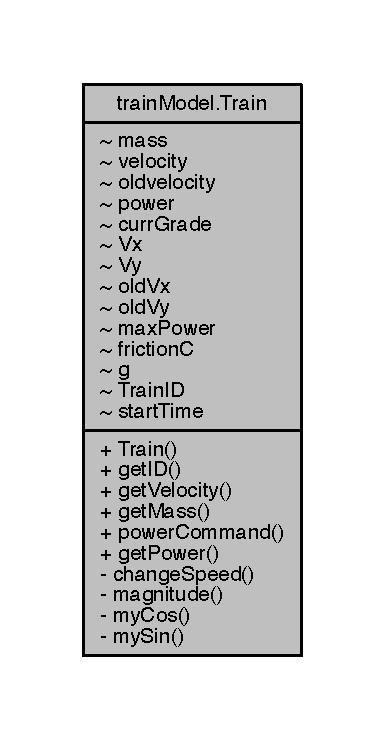
\includegraphics[width=185pt]{classtrainModel_1_1Train__coll__graph}
\end{center}
\end{figure}
\subsection*{Public Member Functions}
\begin{DoxyCompactItemize}
\item 
\hyperlink{classtrainModel_1_1Train_ace267efabb37b0bf7b681af1ddf12690}{Train} (int ID)
\item 
int \hyperlink{classtrainModel_1_1Train_ad29a94a10fad2b26fc32989cd3431850}{get\+ID} ()
\item 
Double \hyperlink{classtrainModel_1_1Train_a1e0b8055a7cbfdf6edbce0ae09273219}{get\+Velocity} ()
\item 
Double \hyperlink{classtrainModel_1_1Train_a6b09bef43b1858aae11d2d02dfd6ffb4}{get\+Mass} ()
\item 
void \hyperlink{classtrainModel_1_1Train_acd407d7861947859becc92cc1fb5c937}{power\+Command} (Double new\+Power)
\item 
Double \hyperlink{classtrainModel_1_1Train_a48de926812a7be60f611f37dd738a47a}{get\+Power} ()
\end{DoxyCompactItemize}
\subsection*{Package Attributes}
\begin{DoxyCompactItemize}
\item 
Double \hyperlink{classtrainModel_1_1Train_a81b0e04517e168bb5381c165ae068210}{mass}
\item 
Double \hyperlink{classtrainModel_1_1Train_ae0f4175c59c12b888c12587a7c64768e}{velocity}
\item 
Double \hyperlink{classtrainModel_1_1Train_ae03291f43c83952e1452fc0d4031fd16}{oldvelocity}
\item 
Double \hyperlink{classtrainModel_1_1Train_ad650d5136222ba3bdf3272f7ea908ab8}{power}
\item 
Double \hyperlink{classtrainModel_1_1Train_a5b231e967030c5143f13efe7b993751c}{curr\+Grade}
\item 
Double \hyperlink{classtrainModel_1_1Train_ad934166ba4e535a033771eaa5b758c42}{Vx}
\item 
Double \hyperlink{classtrainModel_1_1Train_a60dfaef269a503c72700a405a1ba465e}{Vy}
\item 
Double \hyperlink{classtrainModel_1_1Train_aa81f6ae6deb7fb21c94d8af2b37c61f7}{old\+Vx}
\item 
Double \hyperlink{classtrainModel_1_1Train_a0fc26e7ed97d3d83749fe5fa1156812d}{old\+Vy}
\item 
Double \hyperlink{classtrainModel_1_1Train_aeb7f280cf048608f22c6c0ec8544b7c0}{max\+Power} = 120000.\+00
\item 
Double \hyperlink{classtrainModel_1_1Train_aa660ffb9dcd63059f8e9e3c282ae5cae}{frictionC} = 0.\+42
\item 
Double \hyperlink{classtrainModel_1_1Train_a163d398b8467040f820386cff418e8ac}{g} = 9.\+8
\item 
int \hyperlink{classtrainModel_1_1Train_af258aa71b69e7f7878164cb40d0422ab}{Train\+ID}
\item 
Double \hyperlink{classtrainModel_1_1Train_ab498b674cbe1209d6903ff1d79c600e8}{start\+Time}
\end{DoxyCompactItemize}
\subsection*{Private Member Functions}
\begin{DoxyCompactItemize}
\item 
void \hyperlink{classtrainModel_1_1Train_a1ab142928b7f173d3593a2482c3fcdec}{change\+Speed} (Double Fapp)
\item 
Double \hyperlink{classtrainModel_1_1Train_a0eabada19eac6142f2f174109de8551a}{magnitude} (Double x, Double y)
\item 
Double \hyperlink{classtrainModel_1_1Train_affdb8691217f966a1cd2cbbeda59b005}{my\+Cos} (Double deg)
\item 
Double \hyperlink{classtrainModel_1_1Train_a4a42a9493ba183b960f3e92fe2430475}{my\+Sin} (Double deg)
\end{DoxyCompactItemize}


\subsection{Constructor \& Destructor Documentation}
\mbox{\Hypertarget{classtrainModel_1_1Train_ace267efabb37b0bf7b681af1ddf12690}\label{classtrainModel_1_1Train_ace267efabb37b0bf7b681af1ddf12690}} 
\index{train\+Model\+::\+Train@{train\+Model\+::\+Train}!Train@{Train}}
\index{Train@{Train}!train\+Model\+::\+Train@{train\+Model\+::\+Train}}
\subsubsection{\texorpdfstring{Train()}{Train()}}
{\footnotesize\ttfamily train\+Model.\+Train.\+Train (\begin{DoxyParamCaption}\item[{int}]{ID }\end{DoxyParamCaption})}



\subsection{Member Function Documentation}
\mbox{\Hypertarget{classtrainModel_1_1Train_a1ab142928b7f173d3593a2482c3fcdec}\label{classtrainModel_1_1Train_a1ab142928b7f173d3593a2482c3fcdec}} 
\index{train\+Model\+::\+Train@{train\+Model\+::\+Train}!change\+Speed@{change\+Speed}}
\index{change\+Speed@{change\+Speed}!train\+Model\+::\+Train@{train\+Model\+::\+Train}}
\subsubsection{\texorpdfstring{change\+Speed()}{changeSpeed()}}
{\footnotesize\ttfamily void train\+Model.\+Train.\+change\+Speed (\begin{DoxyParamCaption}\item[{Double}]{Fapp }\end{DoxyParamCaption})\hspace{0.3cm}{\ttfamily [private]}}

\mbox{\Hypertarget{classtrainModel_1_1Train_ad29a94a10fad2b26fc32989cd3431850}\label{classtrainModel_1_1Train_ad29a94a10fad2b26fc32989cd3431850}} 
\index{train\+Model\+::\+Train@{train\+Model\+::\+Train}!get\+ID@{get\+ID}}
\index{get\+ID@{get\+ID}!train\+Model\+::\+Train@{train\+Model\+::\+Train}}
\subsubsection{\texorpdfstring{get\+I\+D()}{getID()}}
{\footnotesize\ttfamily int train\+Model.\+Train.\+get\+ID (\begin{DoxyParamCaption}{ }\end{DoxyParamCaption})}

\mbox{\Hypertarget{classtrainModel_1_1Train_a6b09bef43b1858aae11d2d02dfd6ffb4}\label{classtrainModel_1_1Train_a6b09bef43b1858aae11d2d02dfd6ffb4}} 
\index{train\+Model\+::\+Train@{train\+Model\+::\+Train}!get\+Mass@{get\+Mass}}
\index{get\+Mass@{get\+Mass}!train\+Model\+::\+Train@{train\+Model\+::\+Train}}
\subsubsection{\texorpdfstring{get\+Mass()}{getMass()}}
{\footnotesize\ttfamily Double train\+Model.\+Train.\+get\+Mass (\begin{DoxyParamCaption}{ }\end{DoxyParamCaption})}

\mbox{\Hypertarget{classtrainModel_1_1Train_a48de926812a7be60f611f37dd738a47a}\label{classtrainModel_1_1Train_a48de926812a7be60f611f37dd738a47a}} 
\index{train\+Model\+::\+Train@{train\+Model\+::\+Train}!get\+Power@{get\+Power}}
\index{get\+Power@{get\+Power}!train\+Model\+::\+Train@{train\+Model\+::\+Train}}
\subsubsection{\texorpdfstring{get\+Power()}{getPower()}}
{\footnotesize\ttfamily Double train\+Model.\+Train.\+get\+Power (\begin{DoxyParamCaption}{ }\end{DoxyParamCaption})}

\mbox{\Hypertarget{classtrainModel_1_1Train_a1e0b8055a7cbfdf6edbce0ae09273219}\label{classtrainModel_1_1Train_a1e0b8055a7cbfdf6edbce0ae09273219}} 
\index{train\+Model\+::\+Train@{train\+Model\+::\+Train}!get\+Velocity@{get\+Velocity}}
\index{get\+Velocity@{get\+Velocity}!train\+Model\+::\+Train@{train\+Model\+::\+Train}}
\subsubsection{\texorpdfstring{get\+Velocity()}{getVelocity()}}
{\footnotesize\ttfamily Double train\+Model.\+Train.\+get\+Velocity (\begin{DoxyParamCaption}{ }\end{DoxyParamCaption})}

\mbox{\Hypertarget{classtrainModel_1_1Train_a0eabada19eac6142f2f174109de8551a}\label{classtrainModel_1_1Train_a0eabada19eac6142f2f174109de8551a}} 
\index{train\+Model\+::\+Train@{train\+Model\+::\+Train}!magnitude@{magnitude}}
\index{magnitude@{magnitude}!train\+Model\+::\+Train@{train\+Model\+::\+Train}}
\subsubsection{\texorpdfstring{magnitude()}{magnitude()}}
{\footnotesize\ttfamily Double train\+Model.\+Train.\+magnitude (\begin{DoxyParamCaption}\item[{Double}]{x,  }\item[{Double}]{y }\end{DoxyParamCaption})\hspace{0.3cm}{\ttfamily [private]}}

\mbox{\Hypertarget{classtrainModel_1_1Train_affdb8691217f966a1cd2cbbeda59b005}\label{classtrainModel_1_1Train_affdb8691217f966a1cd2cbbeda59b005}} 
\index{train\+Model\+::\+Train@{train\+Model\+::\+Train}!my\+Cos@{my\+Cos}}
\index{my\+Cos@{my\+Cos}!train\+Model\+::\+Train@{train\+Model\+::\+Train}}
\subsubsection{\texorpdfstring{my\+Cos()}{myCos()}}
{\footnotesize\ttfamily Double train\+Model.\+Train.\+my\+Cos (\begin{DoxyParamCaption}\item[{Double}]{deg }\end{DoxyParamCaption})\hspace{0.3cm}{\ttfamily [private]}}

\mbox{\Hypertarget{classtrainModel_1_1Train_a4a42a9493ba183b960f3e92fe2430475}\label{classtrainModel_1_1Train_a4a42a9493ba183b960f3e92fe2430475}} 
\index{train\+Model\+::\+Train@{train\+Model\+::\+Train}!my\+Sin@{my\+Sin}}
\index{my\+Sin@{my\+Sin}!train\+Model\+::\+Train@{train\+Model\+::\+Train}}
\subsubsection{\texorpdfstring{my\+Sin()}{mySin()}}
{\footnotesize\ttfamily Double train\+Model.\+Train.\+my\+Sin (\begin{DoxyParamCaption}\item[{Double}]{deg }\end{DoxyParamCaption})\hspace{0.3cm}{\ttfamily [private]}}

\mbox{\Hypertarget{classtrainModel_1_1Train_acd407d7861947859becc92cc1fb5c937}\label{classtrainModel_1_1Train_acd407d7861947859becc92cc1fb5c937}} 
\index{train\+Model\+::\+Train@{train\+Model\+::\+Train}!power\+Command@{power\+Command}}
\index{power\+Command@{power\+Command}!train\+Model\+::\+Train@{train\+Model\+::\+Train}}
\subsubsection{\texorpdfstring{power\+Command()}{powerCommand()}}
{\footnotesize\ttfamily void train\+Model.\+Train.\+power\+Command (\begin{DoxyParamCaption}\item[{Double}]{new\+Power }\end{DoxyParamCaption})}



\subsection{Member Data Documentation}
\mbox{\Hypertarget{classtrainModel_1_1Train_a5b231e967030c5143f13efe7b993751c}\label{classtrainModel_1_1Train_a5b231e967030c5143f13efe7b993751c}} 
\index{train\+Model\+::\+Train@{train\+Model\+::\+Train}!curr\+Grade@{curr\+Grade}}
\index{curr\+Grade@{curr\+Grade}!train\+Model\+::\+Train@{train\+Model\+::\+Train}}
\subsubsection{\texorpdfstring{curr\+Grade}{currGrade}}
{\footnotesize\ttfamily Double train\+Model.\+Train.\+curr\+Grade\hspace{0.3cm}{\ttfamily [package]}}

\mbox{\Hypertarget{classtrainModel_1_1Train_aa660ffb9dcd63059f8e9e3c282ae5cae}\label{classtrainModel_1_1Train_aa660ffb9dcd63059f8e9e3c282ae5cae}} 
\index{train\+Model\+::\+Train@{train\+Model\+::\+Train}!frictionC@{frictionC}}
\index{frictionC@{frictionC}!train\+Model\+::\+Train@{train\+Model\+::\+Train}}
\subsubsection{\texorpdfstring{frictionC}{frictionC}}
{\footnotesize\ttfamily Double train\+Model.\+Train.\+frictionC = 0.\+42\hspace{0.3cm}{\ttfamily [package]}}

\mbox{\Hypertarget{classtrainModel_1_1Train_a163d398b8467040f820386cff418e8ac}\label{classtrainModel_1_1Train_a163d398b8467040f820386cff418e8ac}} 
\index{train\+Model\+::\+Train@{train\+Model\+::\+Train}!g@{g}}
\index{g@{g}!train\+Model\+::\+Train@{train\+Model\+::\+Train}}
\subsubsection{\texorpdfstring{g}{g}}
{\footnotesize\ttfamily Double train\+Model.\+Train.\+g = 9.\+8\hspace{0.3cm}{\ttfamily [package]}}

\mbox{\Hypertarget{classtrainModel_1_1Train_a81b0e04517e168bb5381c165ae068210}\label{classtrainModel_1_1Train_a81b0e04517e168bb5381c165ae068210}} 
\index{train\+Model\+::\+Train@{train\+Model\+::\+Train}!mass@{mass}}
\index{mass@{mass}!train\+Model\+::\+Train@{train\+Model\+::\+Train}}
\subsubsection{\texorpdfstring{mass}{mass}}
{\footnotesize\ttfamily Double train\+Model.\+Train.\+mass\hspace{0.3cm}{\ttfamily [package]}}

\mbox{\Hypertarget{classtrainModel_1_1Train_aeb7f280cf048608f22c6c0ec8544b7c0}\label{classtrainModel_1_1Train_aeb7f280cf048608f22c6c0ec8544b7c0}} 
\index{train\+Model\+::\+Train@{train\+Model\+::\+Train}!max\+Power@{max\+Power}}
\index{max\+Power@{max\+Power}!train\+Model\+::\+Train@{train\+Model\+::\+Train}}
\subsubsection{\texorpdfstring{max\+Power}{maxPower}}
{\footnotesize\ttfamily Double train\+Model.\+Train.\+max\+Power = 120000.\+00\hspace{0.3cm}{\ttfamily [package]}}

\mbox{\Hypertarget{classtrainModel_1_1Train_ae03291f43c83952e1452fc0d4031fd16}\label{classtrainModel_1_1Train_ae03291f43c83952e1452fc0d4031fd16}} 
\index{train\+Model\+::\+Train@{train\+Model\+::\+Train}!oldvelocity@{oldvelocity}}
\index{oldvelocity@{oldvelocity}!train\+Model\+::\+Train@{train\+Model\+::\+Train}}
\subsubsection{\texorpdfstring{oldvelocity}{oldvelocity}}
{\footnotesize\ttfamily Double train\+Model.\+Train.\+oldvelocity\hspace{0.3cm}{\ttfamily [package]}}

\mbox{\Hypertarget{classtrainModel_1_1Train_aa81f6ae6deb7fb21c94d8af2b37c61f7}\label{classtrainModel_1_1Train_aa81f6ae6deb7fb21c94d8af2b37c61f7}} 
\index{train\+Model\+::\+Train@{train\+Model\+::\+Train}!old\+Vx@{old\+Vx}}
\index{old\+Vx@{old\+Vx}!train\+Model\+::\+Train@{train\+Model\+::\+Train}}
\subsubsection{\texorpdfstring{old\+Vx}{oldVx}}
{\footnotesize\ttfamily Double train\+Model.\+Train.\+old\+Vx\hspace{0.3cm}{\ttfamily [package]}}

\mbox{\Hypertarget{classtrainModel_1_1Train_a0fc26e7ed97d3d83749fe5fa1156812d}\label{classtrainModel_1_1Train_a0fc26e7ed97d3d83749fe5fa1156812d}} 
\index{train\+Model\+::\+Train@{train\+Model\+::\+Train}!old\+Vy@{old\+Vy}}
\index{old\+Vy@{old\+Vy}!train\+Model\+::\+Train@{train\+Model\+::\+Train}}
\subsubsection{\texorpdfstring{old\+Vy}{oldVy}}
{\footnotesize\ttfamily Double train\+Model.\+Train.\+old\+Vy\hspace{0.3cm}{\ttfamily [package]}}

\mbox{\Hypertarget{classtrainModel_1_1Train_ad650d5136222ba3bdf3272f7ea908ab8}\label{classtrainModel_1_1Train_ad650d5136222ba3bdf3272f7ea908ab8}} 
\index{train\+Model\+::\+Train@{train\+Model\+::\+Train}!power@{power}}
\index{power@{power}!train\+Model\+::\+Train@{train\+Model\+::\+Train}}
\subsubsection{\texorpdfstring{power}{power}}
{\footnotesize\ttfamily Double train\+Model.\+Train.\+power\hspace{0.3cm}{\ttfamily [package]}}

\mbox{\Hypertarget{classtrainModel_1_1Train_ab498b674cbe1209d6903ff1d79c600e8}\label{classtrainModel_1_1Train_ab498b674cbe1209d6903ff1d79c600e8}} 
\index{train\+Model\+::\+Train@{train\+Model\+::\+Train}!start\+Time@{start\+Time}}
\index{start\+Time@{start\+Time}!train\+Model\+::\+Train@{train\+Model\+::\+Train}}
\subsubsection{\texorpdfstring{start\+Time}{startTime}}
{\footnotesize\ttfamily Double train\+Model.\+Train.\+start\+Time\hspace{0.3cm}{\ttfamily [package]}}

\mbox{\Hypertarget{classtrainModel_1_1Train_af258aa71b69e7f7878164cb40d0422ab}\label{classtrainModel_1_1Train_af258aa71b69e7f7878164cb40d0422ab}} 
\index{train\+Model\+::\+Train@{train\+Model\+::\+Train}!Train\+ID@{Train\+ID}}
\index{Train\+ID@{Train\+ID}!train\+Model\+::\+Train@{train\+Model\+::\+Train}}
\subsubsection{\texorpdfstring{Train\+ID}{TrainID}}
{\footnotesize\ttfamily int train\+Model.\+Train.\+Train\+ID\hspace{0.3cm}{\ttfamily [package]}}

\mbox{\Hypertarget{classtrainModel_1_1Train_ae0f4175c59c12b888c12587a7c64768e}\label{classtrainModel_1_1Train_ae0f4175c59c12b888c12587a7c64768e}} 
\index{train\+Model\+::\+Train@{train\+Model\+::\+Train}!velocity@{velocity}}
\index{velocity@{velocity}!train\+Model\+::\+Train@{train\+Model\+::\+Train}}
\subsubsection{\texorpdfstring{velocity}{velocity}}
{\footnotesize\ttfamily Double train\+Model.\+Train.\+velocity\hspace{0.3cm}{\ttfamily [package]}}

\mbox{\Hypertarget{classtrainModel_1_1Train_ad934166ba4e535a033771eaa5b758c42}\label{classtrainModel_1_1Train_ad934166ba4e535a033771eaa5b758c42}} 
\index{train\+Model\+::\+Train@{train\+Model\+::\+Train}!Vx@{Vx}}
\index{Vx@{Vx}!train\+Model\+::\+Train@{train\+Model\+::\+Train}}
\subsubsection{\texorpdfstring{Vx}{Vx}}
{\footnotesize\ttfamily Double train\+Model.\+Train.\+Vx\hspace{0.3cm}{\ttfamily [package]}}

\mbox{\Hypertarget{classtrainModel_1_1Train_a60dfaef269a503c72700a405a1ba465e}\label{classtrainModel_1_1Train_a60dfaef269a503c72700a405a1ba465e}} 
\index{train\+Model\+::\+Train@{train\+Model\+::\+Train}!Vy@{Vy}}
\index{Vy@{Vy}!train\+Model\+::\+Train@{train\+Model\+::\+Train}}
\subsubsection{\texorpdfstring{Vy}{Vy}}
{\footnotesize\ttfamily Double train\+Model.\+Train.\+Vy\hspace{0.3cm}{\ttfamily [package]}}



The documentation for this class was generated from the following file\+:\begin{DoxyCompactItemize}
\item 
src/main/java/train\+Model/\hyperlink{Train_8java}{Train.\+java}\end{DoxyCompactItemize}

\hypertarget{classtrain}{}\section{train Class Reference}
\label{classtrain}\index{train@{train}}


Collaboration diagram for train\+:
\nopagebreak
\begin{figure}[H]
\begin{center}
\leavevmode
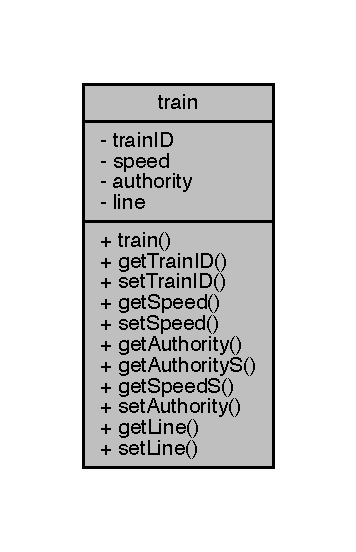
\includegraphics[width=171pt]{classtrain__coll__graph}
\end{center}
\end{figure}
\subsection*{Public Member Functions}
\begin{DoxyCompactItemize}
\item 
\hyperlink{classtrain_ab59e6329c64e077e362640c3c1efd4e3}{train} ()
\item 
String \hyperlink{classtrain_a15b117ba7a9fe96a1713393316884184}{get\+Train\+ID} ()
\item 
void \hyperlink{classtrain_aca453b158d99ac2c56ac31fbd6d23b64}{set\+Train\+ID} (int \hyperlink{classtrain_afd48feba85a8c5bce2fcab13f8e5f709}{train\+ID})
\item 
double \hyperlink{classtrain_add82fa33c54bc9be71bbabb9df4980b4}{get\+Speed} ()
\item 
void \hyperlink{classtrain_aa655ee4487d9476b21faab1e71d816f9}{set\+Speed} (double \hyperlink{classtrain_aae9db61086b60cf549586993da5a29dd}{speed})
\item 
double \hyperlink{classtrain_adaa613d6d0407c1bc75286433ee4492c}{get\+Authority} ()
\item 
String \hyperlink{classtrain_ae60270a74c0afa8710a412d9ddb5c512}{get\+AuthorityS} ()
\item 
String \hyperlink{classtrain_a77ed94ef8762ffab78076216a54d7072}{get\+SpeedS} ()
\item 
void \hyperlink{classtrain_a4fd252f0677dfd05cdbb0dfac79477d1}{set\+Authority} (double \hyperlink{classtrain_ad627ddd59fd3a4e24fd20fbeae490ad6}{authority})
\item 
String \hyperlink{classtrain_a1e506c38b86f07589e8ebe433674d7db}{get\+Line} ()
\item 
void \hyperlink{classtrain_a0c64747d8c11a6b68d802c4159d2911c}{set\+Line} (String \hyperlink{classtrain_a0c5c46d048165fc94a8c259b953ca844}{line})
\end{DoxyCompactItemize}
\subsection*{Private Attributes}
\begin{DoxyCompactItemize}
\item 
int \hyperlink{classtrain_afd48feba85a8c5bce2fcab13f8e5f709}{train\+ID}
\item 
double \hyperlink{classtrain_aae9db61086b60cf549586993da5a29dd}{speed}
\item 
double \hyperlink{classtrain_ad627ddd59fd3a4e24fd20fbeae490ad6}{authority}
\item 
String \hyperlink{classtrain_a0c5c46d048165fc94a8c259b953ca844}{line}
\end{DoxyCompactItemize}


\subsection{Constructor \& Destructor Documentation}
\mbox{\Hypertarget{classtrain_ab59e6329c64e077e362640c3c1efd4e3}\label{classtrain_ab59e6329c64e077e362640c3c1efd4e3}} 
\index{train@{train}!train@{train}}
\index{train@{train}!train@{train}}
\subsubsection{\texorpdfstring{train()}{train()}}
{\footnotesize\ttfamily train.\+train (\begin{DoxyParamCaption}{ }\end{DoxyParamCaption})}



\subsection{Member Function Documentation}
\mbox{\Hypertarget{classtrain_adaa613d6d0407c1bc75286433ee4492c}\label{classtrain_adaa613d6d0407c1bc75286433ee4492c}} 
\index{train@{train}!get\+Authority@{get\+Authority}}
\index{get\+Authority@{get\+Authority}!train@{train}}
\subsubsection{\texorpdfstring{get\+Authority()}{getAuthority()}}
{\footnotesize\ttfamily double train.\+get\+Authority (\begin{DoxyParamCaption}{ }\end{DoxyParamCaption})}

\mbox{\Hypertarget{classtrain_ae60270a74c0afa8710a412d9ddb5c512}\label{classtrain_ae60270a74c0afa8710a412d9ddb5c512}} 
\index{train@{train}!get\+AuthorityS@{get\+AuthorityS}}
\index{get\+AuthorityS@{get\+AuthorityS}!train@{train}}
\subsubsection{\texorpdfstring{get\+Authority\+S()}{getAuthorityS()}}
{\footnotesize\ttfamily String train.\+get\+AuthorityS (\begin{DoxyParamCaption}{ }\end{DoxyParamCaption})}

\mbox{\Hypertarget{classtrain_a1e506c38b86f07589e8ebe433674d7db}\label{classtrain_a1e506c38b86f07589e8ebe433674d7db}} 
\index{train@{train}!get\+Line@{get\+Line}}
\index{get\+Line@{get\+Line}!train@{train}}
\subsubsection{\texorpdfstring{get\+Line()}{getLine()}}
{\footnotesize\ttfamily String train.\+get\+Line (\begin{DoxyParamCaption}{ }\end{DoxyParamCaption})}

\mbox{\Hypertarget{classtrain_add82fa33c54bc9be71bbabb9df4980b4}\label{classtrain_add82fa33c54bc9be71bbabb9df4980b4}} 
\index{train@{train}!get\+Speed@{get\+Speed}}
\index{get\+Speed@{get\+Speed}!train@{train}}
\subsubsection{\texorpdfstring{get\+Speed()}{getSpeed()}}
{\footnotesize\ttfamily double train.\+get\+Speed (\begin{DoxyParamCaption}{ }\end{DoxyParamCaption})}

\mbox{\Hypertarget{classtrain_a77ed94ef8762ffab78076216a54d7072}\label{classtrain_a77ed94ef8762ffab78076216a54d7072}} 
\index{train@{train}!get\+SpeedS@{get\+SpeedS}}
\index{get\+SpeedS@{get\+SpeedS}!train@{train}}
\subsubsection{\texorpdfstring{get\+Speed\+S()}{getSpeedS()}}
{\footnotesize\ttfamily String train.\+get\+SpeedS (\begin{DoxyParamCaption}{ }\end{DoxyParamCaption})}

\mbox{\Hypertarget{classtrain_a15b117ba7a9fe96a1713393316884184}\label{classtrain_a15b117ba7a9fe96a1713393316884184}} 
\index{train@{train}!get\+Train\+ID@{get\+Train\+ID}}
\index{get\+Train\+ID@{get\+Train\+ID}!train@{train}}
\subsubsection{\texorpdfstring{get\+Train\+I\+D()}{getTrainID()}}
{\footnotesize\ttfamily String train.\+get\+Train\+ID (\begin{DoxyParamCaption}{ }\end{DoxyParamCaption})}

\mbox{\Hypertarget{classtrain_a4fd252f0677dfd05cdbb0dfac79477d1}\label{classtrain_a4fd252f0677dfd05cdbb0dfac79477d1}} 
\index{train@{train}!set\+Authority@{set\+Authority}}
\index{set\+Authority@{set\+Authority}!train@{train}}
\subsubsection{\texorpdfstring{set\+Authority()}{setAuthority()}}
{\footnotesize\ttfamily void train.\+set\+Authority (\begin{DoxyParamCaption}\item[{double}]{authority }\end{DoxyParamCaption})}

\mbox{\Hypertarget{classtrain_a0c64747d8c11a6b68d802c4159d2911c}\label{classtrain_a0c64747d8c11a6b68d802c4159d2911c}} 
\index{train@{train}!set\+Line@{set\+Line}}
\index{set\+Line@{set\+Line}!train@{train}}
\subsubsection{\texorpdfstring{set\+Line()}{setLine()}}
{\footnotesize\ttfamily void train.\+set\+Line (\begin{DoxyParamCaption}\item[{String}]{line }\end{DoxyParamCaption})}

\mbox{\Hypertarget{classtrain_aa655ee4487d9476b21faab1e71d816f9}\label{classtrain_aa655ee4487d9476b21faab1e71d816f9}} 
\index{train@{train}!set\+Speed@{set\+Speed}}
\index{set\+Speed@{set\+Speed}!train@{train}}
\subsubsection{\texorpdfstring{set\+Speed()}{setSpeed()}}
{\footnotesize\ttfamily void train.\+set\+Speed (\begin{DoxyParamCaption}\item[{double}]{speed }\end{DoxyParamCaption})}

\mbox{\Hypertarget{classtrain_aca453b158d99ac2c56ac31fbd6d23b64}\label{classtrain_aca453b158d99ac2c56ac31fbd6d23b64}} 
\index{train@{train}!set\+Train\+ID@{set\+Train\+ID}}
\index{set\+Train\+ID@{set\+Train\+ID}!train@{train}}
\subsubsection{\texorpdfstring{set\+Train\+I\+D()}{setTrainID()}}
{\footnotesize\ttfamily void train.\+set\+Train\+ID (\begin{DoxyParamCaption}\item[{int}]{train\+ID }\end{DoxyParamCaption})}



\subsection{Member Data Documentation}
\mbox{\Hypertarget{classtrain_ad627ddd59fd3a4e24fd20fbeae490ad6}\label{classtrain_ad627ddd59fd3a4e24fd20fbeae490ad6}} 
\index{train@{train}!authority@{authority}}
\index{authority@{authority}!train@{train}}
\subsubsection{\texorpdfstring{authority}{authority}}
{\footnotesize\ttfamily double train.\+authority\hspace{0.3cm}{\ttfamily [private]}}

\mbox{\Hypertarget{classtrain_a0c5c46d048165fc94a8c259b953ca844}\label{classtrain_a0c5c46d048165fc94a8c259b953ca844}} 
\index{train@{train}!line@{line}}
\index{line@{line}!train@{train}}
\subsubsection{\texorpdfstring{line}{line}}
{\footnotesize\ttfamily String train.\+line\hspace{0.3cm}{\ttfamily [private]}}

\mbox{\Hypertarget{classtrain_aae9db61086b60cf549586993da5a29dd}\label{classtrain_aae9db61086b60cf549586993da5a29dd}} 
\index{train@{train}!speed@{speed}}
\index{speed@{speed}!train@{train}}
\subsubsection{\texorpdfstring{speed}{speed}}
{\footnotesize\ttfamily double train.\+speed\hspace{0.3cm}{\ttfamily [private]}}

\mbox{\Hypertarget{classtrain_afd48feba85a8c5bce2fcab13f8e5f709}\label{classtrain_afd48feba85a8c5bce2fcab13f8e5f709}} 
\index{train@{train}!train\+ID@{train\+ID}}
\index{train\+ID@{train\+ID}!train@{train}}
\subsubsection{\texorpdfstring{train\+ID}{trainID}}
{\footnotesize\ttfamily int train.\+train\+ID\hspace{0.3cm}{\ttfamily [private]}}



The documentation for this class was generated from the following file\+:\begin{DoxyCompactItemize}
\item 
src/main/java/\+C\+T\+C\+\_\+prototype/src/\hyperlink{train_8java}{train.\+java}\end{DoxyCompactItemize}

\hypertarget{classTrainControllerComps_1_1TrainController}{}\section{Train\+Controller\+Comps.\+Train\+Controller Class Reference}
\label{classTrainControllerComps_1_1TrainController}\index{Train\+Controller\+Comps.\+Train\+Controller@{Train\+Controller\+Comps.\+Train\+Controller}}


This class is a G\+UI that is used to control a selected train.  




Inheritance diagram for Train\+Controller\+Comps.\+Train\+Controller\+:
\nopagebreak
\begin{figure}[H]
\begin{center}
\leavevmode
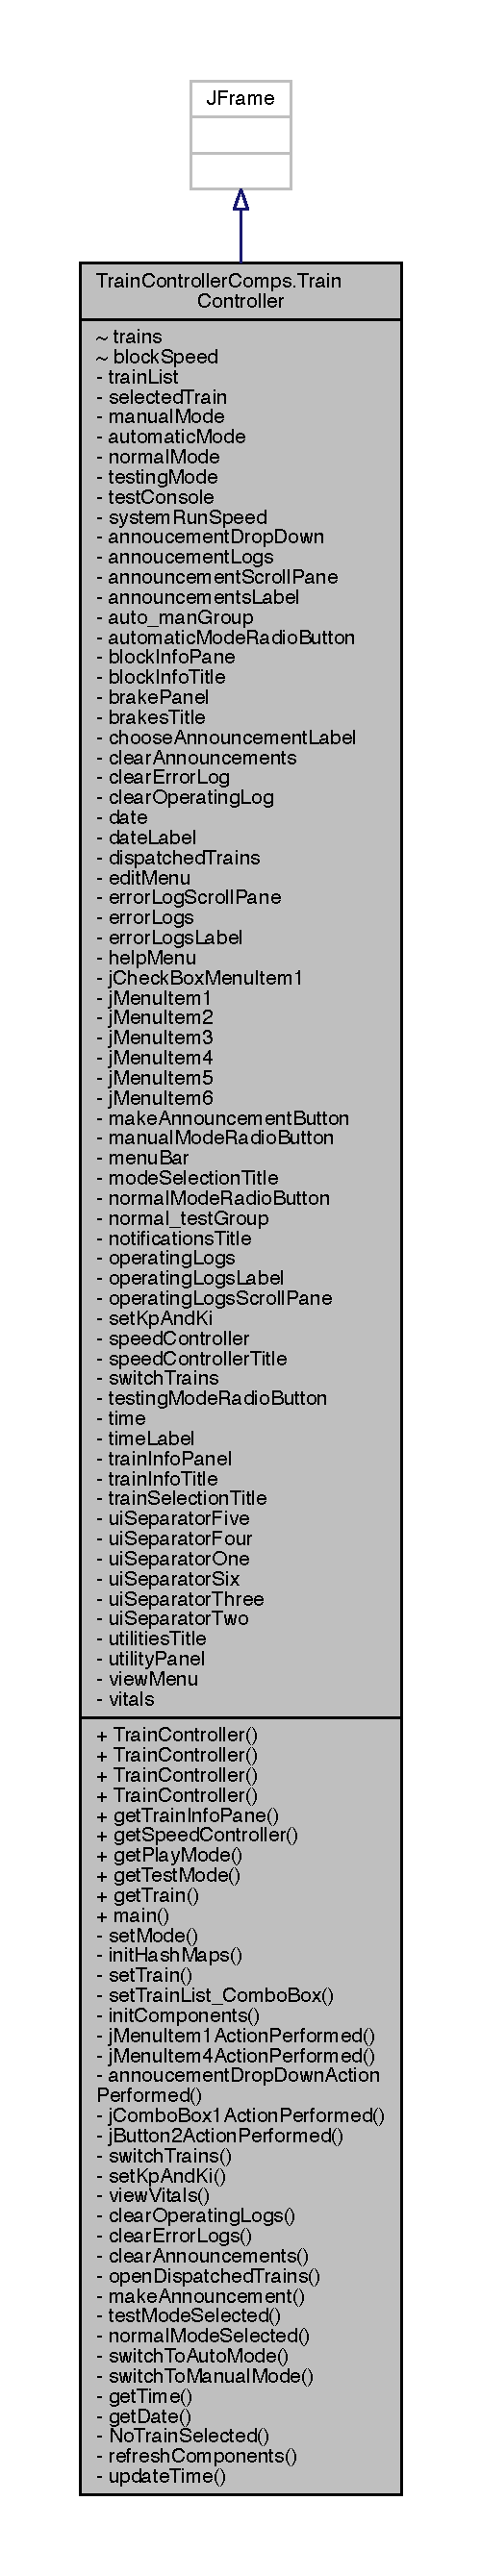
\includegraphics[height=550pt]{classTrainControllerComps_1_1TrainController__inherit__graph}
\end{center}
\end{figure}


Collaboration diagram for Train\+Controller\+Comps.\+Train\+Controller\+:
\nopagebreak
\begin{figure}[H]
\begin{center}
\leavevmode
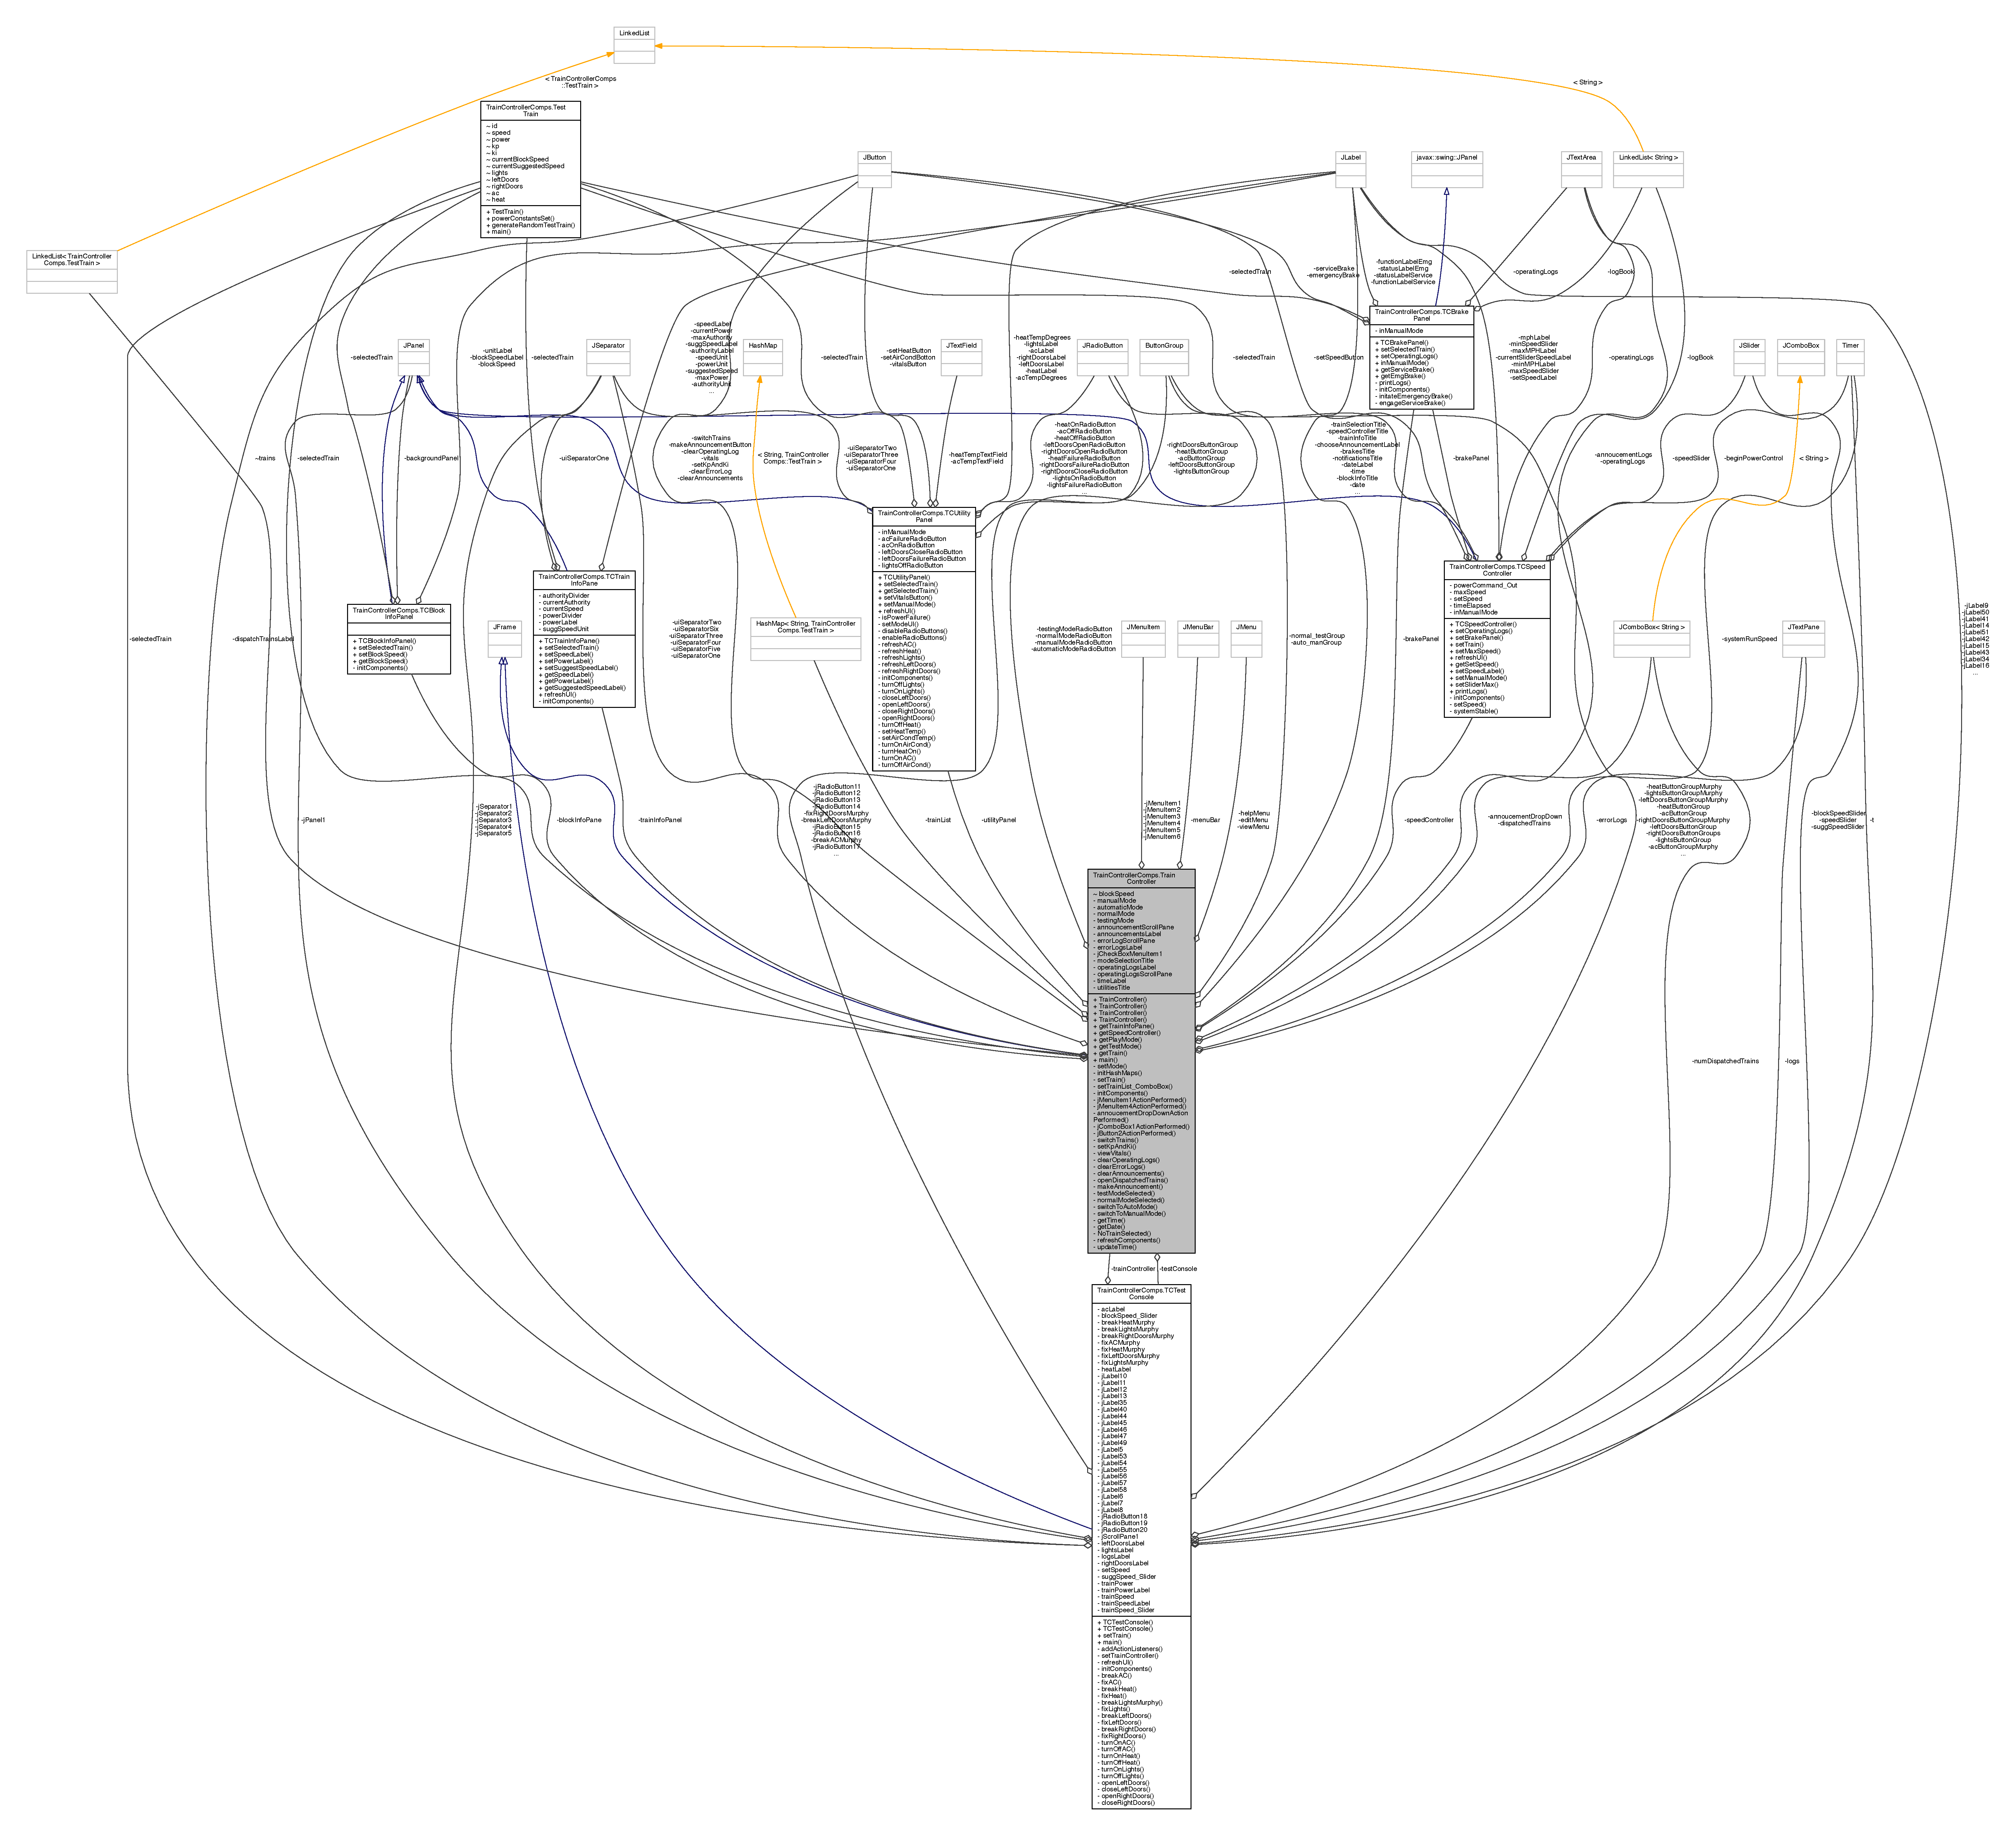
\includegraphics[width=350pt]{classTrainControllerComps_1_1TrainController__coll__graph}
\end{center}
\end{figure}
\subsection*{Public Member Functions}
\begin{DoxyCompactItemize}
\item 
\hyperlink{classTrainControllerComps_1_1TrainController_ad8203c295c6057d7b33da675227cd861}{Train\+Controller} ()
\begin{DoxyCompactList}\small\item\em Constructor that creates a Train Controller. \end{DoxyCompactList}\item 
\hyperlink{classTrainControllerComps_1_1TrainController_a3344359acd0fcf8829763360fbe0a68a}{Train\+Controller} (\hyperlink{classTrainControllerComps_1_1TestTrain}{Test\+Train} \hyperlink{classtrain}{train})
\begin{DoxyCompactList}\small\item\em Constructor that creates a Train Controller for a give train in Manual and Normal mode. \end{DoxyCompactList}\item 
\hyperlink{classTrainControllerComps_1_1TrainController_aff04f9677f4ac86f806e8a909bf9d511}{Train\+Controller} (String play\+Mode, String test\+Mode)
\begin{DoxyCompactList}\small\item\em Constructor that creates a Train Controller in a given mode. \end{DoxyCompactList}\item 
\hyperlink{classTrainControllerComps_1_1TrainController_a95ed9487bd1f1511c0718a13caa1d573}{Train\+Controller} (\hyperlink{classTrainControllerComps_1_1TestTrain}{Test\+Train} \hyperlink{classtrain}{train}, String play\+Mode, String test\+Mode)
\begin{DoxyCompactList}\small\item\em Constructor that creates a Train Controller in a given Test and Play mode with a given train. \end{DoxyCompactList}\item 
\hyperlink{classTrainControllerComps_1_1TCTrainInfoPane}{T\+C\+Train\+Info\+Pane} \hyperlink{classTrainControllerComps_1_1TrainController_ade09a96255871c37628faf44250981fe}{get\+Train\+Info\+Pane} ()
\begin{DoxyCompactList}\small\item\em Retrieves the Train\+Info\+Panel of the Train Controller. \end{DoxyCompactList}\item 
\hyperlink{classTrainControllerComps_1_1TCSpeedController}{T\+C\+Speed\+Controller} \hyperlink{classTrainControllerComps_1_1TrainController_a563558b783b64d38ec5bc7f2bbd87930}{get\+Speed\+Controller} ()
\begin{DoxyCompactList}\small\item\em Retrieves the Speed\+Controller component of the Train Controller. \end{DoxyCompactList}\item 
String \hyperlink{classTrainControllerComps_1_1TrainController_af94f38bb5536923926d19272bfb5f0f2}{get\+Play\+Mode} ()
\begin{DoxyCompactList}\small\item\em Retrieves which Play mode the Train Controller is in. \end{DoxyCompactList}\item 
String \hyperlink{classTrainControllerComps_1_1TrainController_ad99a5958c029bc81fd2f28b386c7699e}{get\+Test\+Mode} ()
\begin{DoxyCompactList}\small\item\em Retrieves which Test mode the Train Controller is in. \end{DoxyCompactList}\item 
\hyperlink{classTrainControllerComps_1_1TestTrain}{Test\+Train} \hyperlink{classTrainControllerComps_1_1TrainController_aaa1cf5d5d3cae08191c34c680943f5f0}{get\+Train} ()
\begin{DoxyCompactList}\small\item\em Retrieves the selected train that the Train Controller is controlling. \end{DoxyCompactList}\end{DoxyCompactItemize}
\subsection*{Static Public Member Functions}
\begin{DoxyCompactItemize}
\item 
static void \hyperlink{classTrainControllerComps_1_1TrainController_acd05ad401373dbc58de1dc6927aff7ec}{main} (String args\mbox{[}$\,$\mbox{]})
\end{DoxyCompactItemize}
\subsection*{Package Attributes}
\begin{DoxyCompactItemize}
\item 
Linked\+List$<$ \hyperlink{classTrainControllerComps_1_1TestTrain}{Test\+Train} $>$ \hyperlink{classTrainControllerComps_1_1TrainController_ab69fa78b5560ce5fa8099162e3bc0761}{trains} = \hyperlink{classTrainControllerComps_1_1TestTrain_a9ac49f75c523af590e04e6feec2b2b0d}{Test\+Train.\+generate\+Random\+Test\+Train}(10)
\item 
double \hyperlink{classTrainControllerComps_1_1TrainController_a7148b1a765fb137613943debe6131592}{block\+Speed} = 80.\+0
\end{DoxyCompactItemize}
\subsection*{Private Member Functions}
\begin{DoxyCompactItemize}
\item 
void \hyperlink{classTrainControllerComps_1_1TrainController_a5f7d0db2d1b3da0c43a85bc0ca38f9a4}{set\+Mode} (String play\+Mode, String test\+Mode)
\begin{DoxyCompactList}\small\item\em Sets the modes of the Train Controller. \end{DoxyCompactList}\item 
void \hyperlink{classTrainControllerComps_1_1TrainController_ab44cad6ee65d5a8536ae1df5a34cd58a}{init\+Hash\+Maps} ()
\begin{DoxyCompactList}\small\item\em Takes the list of dispatched trains, and stores them in a Hash\+Map with the key-\/value pair as the train\textquotesingle{}s id and the train object. \end{DoxyCompactList}\item 
void \hyperlink{classTrainControllerComps_1_1TrainController_a3866dec9cadf09228d1fc1173f824035}{set\+Train} (\hyperlink{classTrainControllerComps_1_1TestTrain}{Test\+Train} \hyperlink{classtrain}{train})
\begin{DoxyCompactList}\small\item\em Sets the selected train that the Train Controller will be controlling. \end{DoxyCompactList}\item 
void \hyperlink{classTrainControllerComps_1_1TrainController_af0888d1788e5b00933e77de1809b157b}{set\+Train\+List\+\_\+\+Combo\+Box} ()
\begin{DoxyCompactList}\small\item\em Updates the combo box that contains the dispatched trains. \end{DoxyCompactList}\item 
void \hyperlink{classTrainControllerComps_1_1TrainController_a32ab56235b79bdc3abeacc716c582a7e}{init\+Components} ()
\begin{DoxyCompactList}\small\item\em This method is called from within the constructor to initialize the form. \end{DoxyCompactList}\item 
void \hyperlink{classTrainControllerComps_1_1TrainController_adc8b31c6a0be0f6e41870ef47d53eea6}{j\+Menu\+Item1\+Action\+Performed} (java.\+awt.\+event.\+Action\+Event evt)
\item 
void \hyperlink{classTrainControllerComps_1_1TrainController_aca246fade255ed4452cfffc56aba65c2}{j\+Menu\+Item4\+Action\+Performed} (java.\+awt.\+event.\+Action\+Event evt)
\item 
void \hyperlink{classTrainControllerComps_1_1TrainController_aa9ea2b3c1f1b0aaf9b8f8bd3bd473df9}{annoucement\+Drop\+Down\+Action\+Performed} (java.\+awt.\+event.\+Action\+Event evt)
\item 
void \hyperlink{classTrainControllerComps_1_1TrainController_aabe5156b678079c215181d75ad07a5a3}{j\+Combo\+Box1\+Action\+Performed} (java.\+awt.\+event.\+Action\+Event evt)
\item 
void \hyperlink{classTrainControllerComps_1_1TrainController_a4cf8486cd8da8038fcb71bb1f55d5fa2}{j\+Button2\+Action\+Performed} (java.\+awt.\+event.\+Action\+Event evt)
\item 
void \hyperlink{classTrainControllerComps_1_1TrainController_a8f8abe1e5e4895201707befb39537bfe}{switch\+Trains} (java.\+awt.\+event.\+Action\+Event evt)
\begin{DoxyCompactList}\small\item\em The action that is performed when the \char`\"{}\+Switch\char`\"{} button is pressed. \end{DoxyCompactList}\item 
void \hyperlink{classTrainControllerComps_1_1TrainController_a8b2ce51ec862cda594c72c0b9f7ef3a4}{set\+Kp\+And\+Ki} (java.\+awt.\+event.\+Action\+Event evt)
\begin{DoxyCompactList}\small\item\em Opens up the Engineering Panel so the engineer can change the Kp and Ki manually. \end{DoxyCompactList}\item 
void \hyperlink{classTrainControllerComps_1_1TrainController_ac82b3d9b38e4f9401242eace87b56d97}{view\+Vitals} (java.\+awt.\+event.\+Action\+Event evt)
\begin{DoxyCompactList}\small\item\em Opens up the Failures Panel so that the train\textquotesingle{}s vitals can be viewed. \end{DoxyCompactList}\item 
void \hyperlink{classTrainControllerComps_1_1TrainController_abd14bbac0df7bd4207a2cdf76854802c}{clear\+Operating\+Logs} (java.\+awt.\+event.\+Action\+Event evt)
\begin{DoxyCompactList}\small\item\em Clears the text of the Operating Logs. \end{DoxyCompactList}\item 
void \hyperlink{classTrainControllerComps_1_1TrainController_a7b660e7359f41a2b4cb40e828332abdd}{clear\+Error\+Logs} (java.\+awt.\+event.\+Action\+Event evt)
\begin{DoxyCompactList}\small\item\em Clears the text of the Error Logs. \end{DoxyCompactList}\item 
void \hyperlink{classTrainControllerComps_1_1TrainController_ac2865f3988db31c31b26b7be49289149}{clear\+Announcements} (java.\+awt.\+event.\+Action\+Event evt)
\begin{DoxyCompactList}\small\item\em Clears the text of the Announcement Logs. \end{DoxyCompactList}\item 
void \hyperlink{classTrainControllerComps_1_1TrainController_a917139f8b8d210b2093f8249ef58eff1}{open\+Dispatched\+Trains} (java.\+awt.\+event.\+Action\+Event evt)
\begin{DoxyCompactList}\small\item\em Opens a window that displays the list of dispatched trains. \end{DoxyCompactList}\item 
void \hyperlink{classTrainControllerComps_1_1TrainController_a754224a8b34116cffd0c39ed93a92f5e}{make\+Announcement} (java.\+awt.\+event.\+Action\+Event evt)
\begin{DoxyCompactList}\small\item\em Prints the announcement that is selected by the Announcement Combo Box to the Announcement Logs. \end{DoxyCompactList}\item 
void \hyperlink{classTrainControllerComps_1_1TrainController_abf8b94be97c22b9811d9103e880a58a3}{test\+Mode\+Selected} (java.\+awt.\+event.\+Action\+Event evt)
\begin{DoxyCompactList}\small\item\em Opens up the Test Console when the Testing mode radio button is clicked. \end{DoxyCompactList}\item 
void \hyperlink{classTrainControllerComps_1_1TrainController_add9a237c1fd6d40484f79d43f22517a0}{normal\+Mode\+Selected} (java.\+awt.\+event.\+Action\+Event evt)
\item 
void \hyperlink{classTrainControllerComps_1_1TrainController_ad0b5d77b76c1544d73359a2997071e78}{switch\+To\+Auto\+Mode} (java.\+awt.\+event.\+Action\+Event evt)
\item 
void \hyperlink{classTrainControllerComps_1_1TrainController_a48dfa3386bc22a0ad919ed3911fc85c7}{switch\+To\+Manual\+Mode} (java.\+awt.\+event.\+Action\+Event evt)
\item 
String \hyperlink{classTrainControllerComps_1_1TrainController_a3f90a62fe4293ebe0f23e7b2e0d5eb69}{get\+Time} ()
\begin{DoxyCompactList}\small\item\em Returns the current time of the system in \char`\"{}\+H\+H\+:mm\+:ss a\char`\"{} format. \end{DoxyCompactList}\item 
String \hyperlink{classTrainControllerComps_1_1TrainController_a271b08d280e582a223b242674bca995f}{get\+Date} ()
\begin{DoxyCompactList}\small\item\em Returns the current time of the system in \char`\"{}\+M\+M/dd/yyyy\char`\"{} format. \end{DoxyCompactList}\item 
boolean \hyperlink{classTrainControllerComps_1_1TrainController_a9d02501f35c2c6b12ffcc30fb4ad16e7}{No\+Train\+Selected} ()
\begin{DoxyCompactList}\small\item\em Checks if there is a selected train or not. \end{DoxyCompactList}\item 
void \hyperlink{classTrainControllerComps_1_1TrainController_a11a6391123f16da8974dcb65acfaf6c0}{refresh\+Components} ()
\begin{DoxyCompactList}\small\item\em Populates the other components of the Train Controller with the information from the selected train. \end{DoxyCompactList}\item 
void \hyperlink{classTrainControllerComps_1_1TrainController_a753f8f5e9ded45498bdf4188544ff8f9}{update\+Time} ()
\begin{DoxyCompactList}\small\item\em Updates the time and date label of the Train Controller. \end{DoxyCompactList}\end{DoxyCompactItemize}
\subsection*{Private Attributes}
\begin{DoxyCompactItemize}
\item 
Hash\+Map$<$ String, \hyperlink{classTrainControllerComps_1_1TestTrain}{Test\+Train} $>$ \hyperlink{classTrainControllerComps_1_1TrainController_aa9bf2d499464b851e25a5dff388ac94c}{train\+List} = new Hash\+Map$<$String, \hyperlink{classTrainControllerComps_1_1TestTrain}{Test\+Train}$>$()
\item 
\hyperlink{classTrainControllerComps_1_1TestTrain}{Test\+Train} \hyperlink{classTrainControllerComps_1_1TrainController_a8b62cd0090f30fd462d0f84f2bb438a6}{selected\+Train}
\item 
boolean \hyperlink{classTrainControllerComps_1_1TrainController_a68037de65ddc19a31b33d7886474b2d6}{manual\+Mode}
\item 
boolean \hyperlink{classTrainControllerComps_1_1TrainController_ad44c875aa9769f31a25410ea646f939d}{automatic\+Mode}
\item 
boolean \hyperlink{classTrainControllerComps_1_1TrainController_a41985d846631a29f3d90db549d52a922}{normal\+Mode}
\item 
boolean \hyperlink{classTrainControllerComps_1_1TrainController_ab1a7579a2577d5ae7aeb101b2ca9a022}{testing\+Mode}
\item 
\hyperlink{classTrainControllerComps_1_1TCTestConsole}{T\+C\+Test\+Console} \hyperlink{classTrainControllerComps_1_1TrainController_a585f001dc5e1a8e61d777a9a7dbe7734}{test\+Console} = null
\item 
Timer \hyperlink{classTrainControllerComps_1_1TrainController_af6689b889f359a3305af139f76d71409}{system\+Run\+Speed}
\item 
javax.\+swing.\+J\+Combo\+Box$<$ String $>$ \hyperlink{classTrainControllerComps_1_1TrainController_a06551cd4e6a89d9212acf3c76ea2cd42}{annoucement\+Drop\+Down}
\item 
javax.\+swing.\+J\+Text\+Area \hyperlink{classTrainControllerComps_1_1TrainController_ae3d731529db9f86e55f700db1796af58}{annoucement\+Logs}
\item 
javax.\+swing.\+J\+Scroll\+Pane \hyperlink{classTrainControllerComps_1_1TrainController_a389289f396cc6cc64425b57b4dbec510}{announcement\+Scroll\+Pane}
\item 
javax.\+swing.\+J\+Label \hyperlink{classTrainControllerComps_1_1TrainController_a4ebeed63e7e3cf1dc2b835d95cd9746a}{announcements\+Label}
\item 
javax.\+swing.\+Button\+Group \hyperlink{classTrainControllerComps_1_1TrainController_ab5fbed6e441dced7b29d48de0b23dbd8}{auto\+\_\+man\+Group}
\item 
javax.\+swing.\+J\+Radio\+Button \hyperlink{classTrainControllerComps_1_1TrainController_a446930f48715be996557881863b5b1ae}{automatic\+Mode\+Radio\+Button}
\item 
\hyperlink{classTrainControllerComps_1_1TCBlockInfoPanel}{Train\+Controller\+Comps.\+T\+C\+Block\+Info\+Panel} \hyperlink{classTrainControllerComps_1_1TrainController_a2fda59591e4f6e390edcdf49e46b884d}{block\+Info\+Pane}
\item 
javax.\+swing.\+J\+Label \hyperlink{classTrainControllerComps_1_1TrainController_a709b921cc3bd6e2d2cf36383de80d34c}{block\+Info\+Title}
\item 
\hyperlink{classTrainControllerComps_1_1TCBrakePanel}{Train\+Controller\+Comps.\+T\+C\+Brake\+Panel} \hyperlink{classTrainControllerComps_1_1TrainController_a6fef4933adda13e5c7cb947f84ea92d3}{brake\+Panel}
\item 
javax.\+swing.\+J\+Label \hyperlink{classTrainControllerComps_1_1TrainController_a2ab25abd71b987aac0291179ca1642bd}{brakes\+Title}
\item 
javax.\+swing.\+J\+Label \hyperlink{classTrainControllerComps_1_1TrainController_ad6c724ce157d7a176bc734b843d4fabd}{choose\+Announcement\+Label}
\item 
javax.\+swing.\+J\+Button \hyperlink{classTrainControllerComps_1_1TrainController_a7bacd9a12dc33d521f2403eb6f843b43}{clear\+Announcements}
\item 
javax.\+swing.\+J\+Button \hyperlink{classTrainControllerComps_1_1TrainController_a8b37eb23080104688c7bda4360f2e8b8}{clear\+Error\+Log}
\item 
javax.\+swing.\+J\+Button \hyperlink{classTrainControllerComps_1_1TrainController_a4d8b68f88d337d250538897ba263f363}{clear\+Operating\+Log}
\item 
javax.\+swing.\+J\+Label \hyperlink{classTrainControllerComps_1_1TrainController_a934803a9f364951d6983afb3c9773cd9}{date}
\item 
javax.\+swing.\+J\+Label \hyperlink{classTrainControllerComps_1_1TrainController_aedfae9b0a9b925ec4af68b1139129edf}{date\+Label}
\item 
javax.\+swing.\+J\+Combo\+Box$<$ String $>$ \hyperlink{classTrainControllerComps_1_1TrainController_afe2b3df9629e79d6bcf87cac60ad2410}{dispatched\+Trains}
\item 
javax.\+swing.\+J\+Menu \hyperlink{classTrainControllerComps_1_1TrainController_ab6cca8dbc7f603fa3c6b03e0aa214134}{edit\+Menu}
\item 
javax.\+swing.\+J\+Scroll\+Pane \hyperlink{classTrainControllerComps_1_1TrainController_a46210ac977c8b30bb8b58c3eedab9024}{error\+Log\+Scroll\+Pane}
\item 
javax.\+swing.\+J\+Text\+Pane \hyperlink{classTrainControllerComps_1_1TrainController_aa3697c9e16c0ef456c46177a4e98d0b8}{error\+Logs}
\item 
javax.\+swing.\+J\+Label \hyperlink{classTrainControllerComps_1_1TrainController_a122803c2eee806971fd54d0cfcc3dba7}{error\+Logs\+Label}
\item 
javax.\+swing.\+J\+Menu \hyperlink{classTrainControllerComps_1_1TrainController_ad3cdb9def09e8d3c58b29669a6c22c48}{help\+Menu}
\item 
javax.\+swing.\+J\+Check\+Box\+Menu\+Item \hyperlink{classTrainControllerComps_1_1TrainController_a92b8d2e249e28491332c93e3b50ba96d}{j\+Check\+Box\+Menu\+Item1}
\item 
javax.\+swing.\+J\+Menu\+Item \hyperlink{classTrainControllerComps_1_1TrainController_a870d25e5ddebf944305cd14cf793ef16}{j\+Menu\+Item1}
\item 
javax.\+swing.\+J\+Menu\+Item \hyperlink{classTrainControllerComps_1_1TrainController_a81595f9f2e98d47672a76667d9a38a61}{j\+Menu\+Item2}
\item 
javax.\+swing.\+J\+Menu\+Item \hyperlink{classTrainControllerComps_1_1TrainController_af7f9bf0cf65e5a00f0013d03e477587b}{j\+Menu\+Item3}
\item 
javax.\+swing.\+J\+Menu\+Item \hyperlink{classTrainControllerComps_1_1TrainController_ab15e90c9e1ea781de06e3c472f9ef332}{j\+Menu\+Item4}
\item 
javax.\+swing.\+J\+Menu\+Item \hyperlink{classTrainControllerComps_1_1TrainController_af2ef143e8969ce9a5197ddf6cc538b0f}{j\+Menu\+Item5}
\item 
javax.\+swing.\+J\+Menu\+Item \hyperlink{classTrainControllerComps_1_1TrainController_a9b96101c9d16dbc6c7ca72a62c3b58fe}{j\+Menu\+Item6}
\item 
javax.\+swing.\+J\+Button \hyperlink{classTrainControllerComps_1_1TrainController_a6986785808de7b43b332992eed9b1c3f}{make\+Announcement\+Button}
\item 
javax.\+swing.\+J\+Radio\+Button \hyperlink{classTrainControllerComps_1_1TrainController_a5e84730a70f6997f9bb3ea171b254809}{manual\+Mode\+Radio\+Button}
\item 
javax.\+swing.\+J\+Menu\+Bar \hyperlink{classTrainControllerComps_1_1TrainController_a43089d5e4ea6c55ecd04454f6b0983fa}{menu\+Bar}
\item 
javax.\+swing.\+J\+Label \hyperlink{classTrainControllerComps_1_1TrainController_a5b0e6ae78fd9fc96546a349ff351387b}{mode\+Selection\+Title}
\item 
javax.\+swing.\+J\+Radio\+Button \hyperlink{classTrainControllerComps_1_1TrainController_aa6f8d34e9769e35ada009950a79a4834}{normal\+Mode\+Radio\+Button}
\item 
javax.\+swing.\+Button\+Group \hyperlink{classTrainControllerComps_1_1TrainController_a69f24a4359e0b261401b9adbddd79354}{normal\+\_\+test\+Group}
\item 
javax.\+swing.\+J\+Label \hyperlink{classTrainControllerComps_1_1TrainController_a49d44ccdd2be91a251a33bbbf57c8b96}{notifications\+Title}
\item 
javax.\+swing.\+J\+Text\+Area \hyperlink{classTrainControllerComps_1_1TrainController_ab88996a242fe55fd7541b534cc8307f1}{operating\+Logs}
\item 
javax.\+swing.\+J\+Label \hyperlink{classTrainControllerComps_1_1TrainController_a7b8385a1b0eba114bdb5e159cccfe6c0}{operating\+Logs\+Label}
\item 
javax.\+swing.\+J\+Scroll\+Pane \hyperlink{classTrainControllerComps_1_1TrainController_abd6dceef250d6c8984db7f465f660035}{operating\+Logs\+Scroll\+Pane}
\item 
javax.\+swing.\+J\+Button \hyperlink{classTrainControllerComps_1_1TrainController_ae3cd4e9b4b470fb95b9da4eba7be53f0}{set\+Kp\+And\+Ki}
\item 
\hyperlink{classTrainControllerComps_1_1TCSpeedController}{Train\+Controller\+Comps.\+T\+C\+Speed\+Controller} \hyperlink{classTrainControllerComps_1_1TrainController_a3367a33be1fb5e4c9e2cd38d10866911}{speed\+Controller}
\item 
javax.\+swing.\+J\+Label \hyperlink{classTrainControllerComps_1_1TrainController_ae0c6b030114914523d6cae9b02f45737}{speed\+Controller\+Title}
\item 
javax.\+swing.\+J\+Button \hyperlink{classTrainControllerComps_1_1TrainController_a8fd16e8e45db6ef47c20117a07549e51}{switch\+Trains}
\item 
javax.\+swing.\+J\+Radio\+Button \hyperlink{classTrainControllerComps_1_1TrainController_a5864e5ed0e60aa89c232d4ad7b0e7954}{testing\+Mode\+Radio\+Button}
\item 
javax.\+swing.\+J\+Label \hyperlink{classTrainControllerComps_1_1TrainController_a4d40c430ee6a9e91944e09e83d4bbed7}{time}
\item 
javax.\+swing.\+J\+Label \hyperlink{classTrainControllerComps_1_1TrainController_adf581e57a02616cd70dfbaa38a63c20e}{time\+Label}
\item 
\hyperlink{classTrainControllerComps_1_1TCTrainInfoPane}{Train\+Controller\+Comps.\+T\+C\+Train\+Info\+Pane} \hyperlink{classTrainControllerComps_1_1TrainController_ae9cc947751b66851084e5ede30ff22d8}{train\+Info\+Panel}
\item 
javax.\+swing.\+J\+Label \hyperlink{classTrainControllerComps_1_1TrainController_a6dee037fa32d66bd5b590102937016ab}{train\+Info\+Title}
\item 
javax.\+swing.\+J\+Label \hyperlink{classTrainControllerComps_1_1TrainController_a70537a86a7aa37c08c621568a214615a}{train\+Selection\+Title}
\item 
javax.\+swing.\+J\+Separator \hyperlink{classTrainControllerComps_1_1TrainController_a764bcddd4c30d6c1357e1133864beb89}{ui\+Separator\+Five}
\item 
javax.\+swing.\+J\+Separator \hyperlink{classTrainControllerComps_1_1TrainController_a259aa3f53d298ba6fcbf61375f7e54e7}{ui\+Separator\+Four}
\item 
javax.\+swing.\+J\+Separator \hyperlink{classTrainControllerComps_1_1TrainController_a858f28af9f58ecfef2383add004068b5}{ui\+Separator\+One}
\item 
javax.\+swing.\+J\+Separator \hyperlink{classTrainControllerComps_1_1TrainController_aaed17d0f6827ff397a5d205c06c85137}{ui\+Separator\+Six}
\item 
javax.\+swing.\+J\+Separator \hyperlink{classTrainControllerComps_1_1TrainController_a63432f91457691ddad36b02cab64196e}{ui\+Separator\+Three}
\item 
javax.\+swing.\+J\+Separator \hyperlink{classTrainControllerComps_1_1TrainController_afaac48e9023208af418495c6ac29ed32}{ui\+Separator\+Two}
\item 
javax.\+swing.\+J\+Label \hyperlink{classTrainControllerComps_1_1TrainController_a2b659931e2555997c14d305e30ad7a92}{utilities\+Title}
\item 
\hyperlink{classTrainControllerComps_1_1TCUtilityPanel}{Train\+Controller\+Comps.\+T\+C\+Utility\+Panel} \hyperlink{classTrainControllerComps_1_1TrainController_a1e6aebc470b0df4ea01c7c8e6e1b32ed}{utility\+Panel}
\item 
javax.\+swing.\+J\+Menu \hyperlink{classTrainControllerComps_1_1TrainController_a000862107a0aac18f4131f2a7b82cfa7}{view\+Menu}
\item 
javax.\+swing.\+J\+Button \hyperlink{classTrainControllerComps_1_1TrainController_a9d5c5a4685b545a56ffba23c5d2c04e2}{vitals}
\end{DoxyCompactItemize}


\subsection{Detailed Description}
This class is a G\+UI that is used to control a selected train. 

The selected train is a Train object that is selected by using the train drop down menu.

This class communicates with other components such as\+:

T\+C\+Train\+Info\+Panel -\/ displays basic train info such as speed, power, authority, and suggested speed. \hyperlink{classTrainControllerComps_1_1TCSpeedController}{T\+C\+Speed\+Controller} -\/ allows the user to control the train\textquotesingle{}s speed.

\begin{DoxyAuthor}{Author}
Andrew Lendacky 
\end{DoxyAuthor}


\subsection{Constructor \& Destructor Documentation}
\mbox{\Hypertarget{classTrainControllerComps_1_1TrainController_ad8203c295c6057d7b33da675227cd861}\label{classTrainControllerComps_1_1TrainController_ad8203c295c6057d7b33da675227cd861}} 
\index{Train\+Controller\+Comps\+::\+Train\+Controller@{Train\+Controller\+Comps\+::\+Train\+Controller}!Train\+Controller@{Train\+Controller}}
\index{Train\+Controller@{Train\+Controller}!Train\+Controller\+Comps\+::\+Train\+Controller@{Train\+Controller\+Comps\+::\+Train\+Controller}}
\subsubsection{\texorpdfstring{Train\+Controller()}{TrainController()}\hspace{0.1cm}{\footnotesize\ttfamily [1/4]}}
{\footnotesize\ttfamily Train\+Controller\+Comps.\+Train\+Controller.\+Train\+Controller (\begin{DoxyParamCaption}{ }\end{DoxyParamCaption})}



Constructor that creates a Train Controller. 

By default the starting mode is \textquotesingle{}Manual\textquotesingle{} mode. \mbox{\Hypertarget{classTrainControllerComps_1_1TrainController_a3344359acd0fcf8829763360fbe0a68a}\label{classTrainControllerComps_1_1TrainController_a3344359acd0fcf8829763360fbe0a68a}} 
\index{Train\+Controller\+Comps\+::\+Train\+Controller@{Train\+Controller\+Comps\+::\+Train\+Controller}!Train\+Controller@{Train\+Controller}}
\index{Train\+Controller@{Train\+Controller}!Train\+Controller\+Comps\+::\+Train\+Controller@{Train\+Controller\+Comps\+::\+Train\+Controller}}
\subsubsection{\texorpdfstring{Train\+Controller()}{TrainController()}\hspace{0.1cm}{\footnotesize\ttfamily [2/4]}}
{\footnotesize\ttfamily Train\+Controller\+Comps.\+Train\+Controller.\+Train\+Controller (\begin{DoxyParamCaption}\item[{\hyperlink{classTrainControllerComps_1_1TestTrain}{Test\+Train}}]{train }\end{DoxyParamCaption})}



Constructor that creates a Train Controller for a give train in Manual and Normal mode. 


\begin{DoxyParams}{Parameters}
{\em train} & the train the controller will launch with. \\
\hline
\end{DoxyParams}
\mbox{\Hypertarget{classTrainControllerComps_1_1TrainController_aff04f9677f4ac86f806e8a909bf9d511}\label{classTrainControllerComps_1_1TrainController_aff04f9677f4ac86f806e8a909bf9d511}} 
\index{Train\+Controller\+Comps\+::\+Train\+Controller@{Train\+Controller\+Comps\+::\+Train\+Controller}!Train\+Controller@{Train\+Controller}}
\index{Train\+Controller@{Train\+Controller}!Train\+Controller\+Comps\+::\+Train\+Controller@{Train\+Controller\+Comps\+::\+Train\+Controller}}
\subsubsection{\texorpdfstring{Train\+Controller()}{TrainController()}\hspace{0.1cm}{\footnotesize\ttfamily [3/4]}}
{\footnotesize\ttfamily Train\+Controller\+Comps.\+Train\+Controller.\+Train\+Controller (\begin{DoxyParamCaption}\item[{String}]{play\+Mode,  }\item[{String}]{test\+Mode }\end{DoxyParamCaption})}



Constructor that creates a Train Controller in a given mode. 


\begin{DoxyParams}{Parameters}
{\em play\+Mode} & the mode (Manual or Automatic) that the Train Controller will launch in. \\
\hline
{\em test\+Mode} & the mode (Normal or Testing) that the Train Controller will launch in. \\
\hline
\end{DoxyParams}
\mbox{\Hypertarget{classTrainControllerComps_1_1TrainController_a95ed9487bd1f1511c0718a13caa1d573}\label{classTrainControllerComps_1_1TrainController_a95ed9487bd1f1511c0718a13caa1d573}} 
\index{Train\+Controller\+Comps\+::\+Train\+Controller@{Train\+Controller\+Comps\+::\+Train\+Controller}!Train\+Controller@{Train\+Controller}}
\index{Train\+Controller@{Train\+Controller}!Train\+Controller\+Comps\+::\+Train\+Controller@{Train\+Controller\+Comps\+::\+Train\+Controller}}
\subsubsection{\texorpdfstring{Train\+Controller()}{TrainController()}\hspace{0.1cm}{\footnotesize\ttfamily [4/4]}}
{\footnotesize\ttfamily Train\+Controller\+Comps.\+Train\+Controller.\+Train\+Controller (\begin{DoxyParamCaption}\item[{\hyperlink{classTrainControllerComps_1_1TestTrain}{Test\+Train}}]{train,  }\item[{String}]{play\+Mode,  }\item[{String}]{test\+Mode }\end{DoxyParamCaption})}



Constructor that creates a Train Controller in a given Test and Play mode with a given train. 


\begin{DoxyParams}{Parameters}
{\em train} & the train the Train Controller with control. \\
\hline
{\em play\+Mode} & the mode (Manual or Automatic) that the Train Controller will launch in. \\
\hline
{\em test\+Mode} & the mode (Normal or Testing) that the Train Controller will launch in. \\
\hline
\end{DoxyParams}


\subsection{Member Function Documentation}
\mbox{\Hypertarget{classTrainControllerComps_1_1TrainController_aa9ea2b3c1f1b0aaf9b8f8bd3bd473df9}\label{classTrainControllerComps_1_1TrainController_aa9ea2b3c1f1b0aaf9b8f8bd3bd473df9}} 
\index{Train\+Controller\+Comps\+::\+Train\+Controller@{Train\+Controller\+Comps\+::\+Train\+Controller}!annoucement\+Drop\+Down\+Action\+Performed@{annoucement\+Drop\+Down\+Action\+Performed}}
\index{annoucement\+Drop\+Down\+Action\+Performed@{annoucement\+Drop\+Down\+Action\+Performed}!Train\+Controller\+Comps\+::\+Train\+Controller@{Train\+Controller\+Comps\+::\+Train\+Controller}}
\subsubsection{\texorpdfstring{annoucement\+Drop\+Down\+Action\+Performed()}{annoucementDropDownActionPerformed()}}
{\footnotesize\ttfamily void Train\+Controller\+Comps.\+Train\+Controller.\+annoucement\+Drop\+Down\+Action\+Performed (\begin{DoxyParamCaption}\item[{java.\+awt.\+event.\+Action\+Event}]{evt }\end{DoxyParamCaption})\hspace{0.3cm}{\ttfamily [private]}}

\mbox{\Hypertarget{classTrainControllerComps_1_1TrainController_ac2865f3988db31c31b26b7be49289149}\label{classTrainControllerComps_1_1TrainController_ac2865f3988db31c31b26b7be49289149}} 
\index{Train\+Controller\+Comps\+::\+Train\+Controller@{Train\+Controller\+Comps\+::\+Train\+Controller}!clear\+Announcements@{clear\+Announcements}}
\index{clear\+Announcements@{clear\+Announcements}!Train\+Controller\+Comps\+::\+Train\+Controller@{Train\+Controller\+Comps\+::\+Train\+Controller}}
\subsubsection{\texorpdfstring{clear\+Announcements()}{clearAnnouncements()}}
{\footnotesize\ttfamily void Train\+Controller\+Comps.\+Train\+Controller.\+clear\+Announcements (\begin{DoxyParamCaption}\item[{java.\+awt.\+event.\+Action\+Event}]{evt }\end{DoxyParamCaption})\hspace{0.3cm}{\ttfamily [private]}}



Clears the text of the Announcement Logs. 


\begin{DoxyParams}{Parameters}
{\em evt} & the sender of the action, i.\+e., the \char`\"{}\+Clear\char`\"{} button. \\
\hline
\end{DoxyParams}
\mbox{\Hypertarget{classTrainControllerComps_1_1TrainController_a7b660e7359f41a2b4cb40e828332abdd}\label{classTrainControllerComps_1_1TrainController_a7b660e7359f41a2b4cb40e828332abdd}} 
\index{Train\+Controller\+Comps\+::\+Train\+Controller@{Train\+Controller\+Comps\+::\+Train\+Controller}!clear\+Error\+Logs@{clear\+Error\+Logs}}
\index{clear\+Error\+Logs@{clear\+Error\+Logs}!Train\+Controller\+Comps\+::\+Train\+Controller@{Train\+Controller\+Comps\+::\+Train\+Controller}}
\subsubsection{\texorpdfstring{clear\+Error\+Logs()}{clearErrorLogs()}}
{\footnotesize\ttfamily void Train\+Controller\+Comps.\+Train\+Controller.\+clear\+Error\+Logs (\begin{DoxyParamCaption}\item[{java.\+awt.\+event.\+Action\+Event}]{evt }\end{DoxyParamCaption})\hspace{0.3cm}{\ttfamily [private]}}



Clears the text of the Error Logs. 


\begin{DoxyParams}{Parameters}
{\em evt} & the sender of the action, i.\+e., the \char`\"{}\+Clear\char`\"{} button. \\
\hline
\end{DoxyParams}
\mbox{\Hypertarget{classTrainControllerComps_1_1TrainController_abd14bbac0df7bd4207a2cdf76854802c}\label{classTrainControllerComps_1_1TrainController_abd14bbac0df7bd4207a2cdf76854802c}} 
\index{Train\+Controller\+Comps\+::\+Train\+Controller@{Train\+Controller\+Comps\+::\+Train\+Controller}!clear\+Operating\+Logs@{clear\+Operating\+Logs}}
\index{clear\+Operating\+Logs@{clear\+Operating\+Logs}!Train\+Controller\+Comps\+::\+Train\+Controller@{Train\+Controller\+Comps\+::\+Train\+Controller}}
\subsubsection{\texorpdfstring{clear\+Operating\+Logs()}{clearOperatingLogs()}}
{\footnotesize\ttfamily void Train\+Controller\+Comps.\+Train\+Controller.\+clear\+Operating\+Logs (\begin{DoxyParamCaption}\item[{java.\+awt.\+event.\+Action\+Event}]{evt }\end{DoxyParamCaption})\hspace{0.3cm}{\ttfamily [private]}}



Clears the text of the Operating Logs. 


\begin{DoxyParams}{Parameters}
{\em evt} & the sender of the action, i.\+e., the \char`\"{}\+Clear\char`\"{} button. \\
\hline
\end{DoxyParams}
\mbox{\Hypertarget{classTrainControllerComps_1_1TrainController_a271b08d280e582a223b242674bca995f}\label{classTrainControllerComps_1_1TrainController_a271b08d280e582a223b242674bca995f}} 
\index{Train\+Controller\+Comps\+::\+Train\+Controller@{Train\+Controller\+Comps\+::\+Train\+Controller}!get\+Date@{get\+Date}}
\index{get\+Date@{get\+Date}!Train\+Controller\+Comps\+::\+Train\+Controller@{Train\+Controller\+Comps\+::\+Train\+Controller}}
\subsubsection{\texorpdfstring{get\+Date()}{getDate()}}
{\footnotesize\ttfamily String Train\+Controller\+Comps.\+Train\+Controller.\+get\+Date (\begin{DoxyParamCaption}{ }\end{DoxyParamCaption})\hspace{0.3cm}{\ttfamily [private]}}



Returns the current time of the system in \char`\"{}\+M\+M/dd/yyyy\char`\"{} format. 

MM -\/ month dd -\/ day yyyy -\/ year

\begin{DoxyReturn}{Returns}
the current date of the system. 
\end{DoxyReturn}
\mbox{\Hypertarget{classTrainControllerComps_1_1TrainController_af94f38bb5536923926d19272bfb5f0f2}\label{classTrainControllerComps_1_1TrainController_af94f38bb5536923926d19272bfb5f0f2}} 
\index{Train\+Controller\+Comps\+::\+Train\+Controller@{Train\+Controller\+Comps\+::\+Train\+Controller}!get\+Play\+Mode@{get\+Play\+Mode}}
\index{get\+Play\+Mode@{get\+Play\+Mode}!Train\+Controller\+Comps\+::\+Train\+Controller@{Train\+Controller\+Comps\+::\+Train\+Controller}}
\subsubsection{\texorpdfstring{get\+Play\+Mode()}{getPlayMode()}}
{\footnotesize\ttfamily String Train\+Controller\+Comps.\+Train\+Controller.\+get\+Play\+Mode (\begin{DoxyParamCaption}{ }\end{DoxyParamCaption})}



Retrieves which Play mode the Train Controller is in. 

\begin{DoxyReturn}{Returns}
returns either Manual if the Train Controller is in manual mode, and \char`\"{}\+Automatic\char`\"{} if in automatic mode. 
\end{DoxyReturn}
\mbox{\Hypertarget{classTrainControllerComps_1_1TrainController_a563558b783b64d38ec5bc7f2bbd87930}\label{classTrainControllerComps_1_1TrainController_a563558b783b64d38ec5bc7f2bbd87930}} 
\index{Train\+Controller\+Comps\+::\+Train\+Controller@{Train\+Controller\+Comps\+::\+Train\+Controller}!get\+Speed\+Controller@{get\+Speed\+Controller}}
\index{get\+Speed\+Controller@{get\+Speed\+Controller}!Train\+Controller\+Comps\+::\+Train\+Controller@{Train\+Controller\+Comps\+::\+Train\+Controller}}
\subsubsection{\texorpdfstring{get\+Speed\+Controller()}{getSpeedController()}}
{\footnotesize\ttfamily \hyperlink{classTrainControllerComps_1_1TCSpeedController}{T\+C\+Speed\+Controller} Train\+Controller\+Comps.\+Train\+Controller.\+get\+Speed\+Controller (\begin{DoxyParamCaption}{ }\end{DoxyParamCaption})}



Retrieves the Speed\+Controller component of the Train Controller. 

\begin{DoxyReturn}{Returns}
returns the Speed Controller panel. 
\end{DoxyReturn}
\mbox{\Hypertarget{classTrainControllerComps_1_1TrainController_ad99a5958c029bc81fd2f28b386c7699e}\label{classTrainControllerComps_1_1TrainController_ad99a5958c029bc81fd2f28b386c7699e}} 
\index{Train\+Controller\+Comps\+::\+Train\+Controller@{Train\+Controller\+Comps\+::\+Train\+Controller}!get\+Test\+Mode@{get\+Test\+Mode}}
\index{get\+Test\+Mode@{get\+Test\+Mode}!Train\+Controller\+Comps\+::\+Train\+Controller@{Train\+Controller\+Comps\+::\+Train\+Controller}}
\subsubsection{\texorpdfstring{get\+Test\+Mode()}{getTestMode()}}
{\footnotesize\ttfamily String Train\+Controller\+Comps.\+Train\+Controller.\+get\+Test\+Mode (\begin{DoxyParamCaption}{ }\end{DoxyParamCaption})}



Retrieves which Test mode the Train Controller is in. 

\begin{DoxyReturn}{Returns}
returns either Testing if the Train Controller is in testing mode, and \char`\"{}\+Normal\char`\"{} if in normal mode. 
\end{DoxyReturn}
\mbox{\Hypertarget{classTrainControllerComps_1_1TrainController_a3f90a62fe4293ebe0f23e7b2e0d5eb69}\label{classTrainControllerComps_1_1TrainController_a3f90a62fe4293ebe0f23e7b2e0d5eb69}} 
\index{Train\+Controller\+Comps\+::\+Train\+Controller@{Train\+Controller\+Comps\+::\+Train\+Controller}!get\+Time@{get\+Time}}
\index{get\+Time@{get\+Time}!Train\+Controller\+Comps\+::\+Train\+Controller@{Train\+Controller\+Comps\+::\+Train\+Controller}}
\subsubsection{\texorpdfstring{get\+Time()}{getTime()}}
{\footnotesize\ttfamily String Train\+Controller\+Comps.\+Train\+Controller.\+get\+Time (\begin{DoxyParamCaption}{ }\end{DoxyParamCaption})\hspace{0.3cm}{\ttfamily [private]}}



Returns the current time of the system in \char`\"{}\+H\+H\+:mm\+:ss a\char`\"{} format. 

HH -\/ the hours mm -\/ the minutes ss -\/ the seconds a -\/ AM or PM

\begin{DoxyReturn}{Returns}
the current system time. 
\end{DoxyReturn}
\mbox{\Hypertarget{classTrainControllerComps_1_1TrainController_aaa1cf5d5d3cae08191c34c680943f5f0}\label{classTrainControllerComps_1_1TrainController_aaa1cf5d5d3cae08191c34c680943f5f0}} 
\index{Train\+Controller\+Comps\+::\+Train\+Controller@{Train\+Controller\+Comps\+::\+Train\+Controller}!get\+Train@{get\+Train}}
\index{get\+Train@{get\+Train}!Train\+Controller\+Comps\+::\+Train\+Controller@{Train\+Controller\+Comps\+::\+Train\+Controller}}
\subsubsection{\texorpdfstring{get\+Train()}{getTrain()}}
{\footnotesize\ttfamily \hyperlink{classTrainControllerComps_1_1TestTrain}{Test\+Train} Train\+Controller\+Comps.\+Train\+Controller.\+get\+Train (\begin{DoxyParamCaption}{ }\end{DoxyParamCaption})}



Retrieves the selected train that the Train Controller is controlling. 

\begin{DoxyReturn}{Returns}
returns the selected train that the Train Controller is controlling, or returns null if no train is selected. 
\end{DoxyReturn}
\mbox{\Hypertarget{classTrainControllerComps_1_1TrainController_ade09a96255871c37628faf44250981fe}\label{classTrainControllerComps_1_1TrainController_ade09a96255871c37628faf44250981fe}} 
\index{Train\+Controller\+Comps\+::\+Train\+Controller@{Train\+Controller\+Comps\+::\+Train\+Controller}!get\+Train\+Info\+Pane@{get\+Train\+Info\+Pane}}
\index{get\+Train\+Info\+Pane@{get\+Train\+Info\+Pane}!Train\+Controller\+Comps\+::\+Train\+Controller@{Train\+Controller\+Comps\+::\+Train\+Controller}}
\subsubsection{\texorpdfstring{get\+Train\+Info\+Pane()}{getTrainInfoPane()}}
{\footnotesize\ttfamily \hyperlink{classTrainControllerComps_1_1TCTrainInfoPane}{T\+C\+Train\+Info\+Pane} Train\+Controller\+Comps.\+Train\+Controller.\+get\+Train\+Info\+Pane (\begin{DoxyParamCaption}{ }\end{DoxyParamCaption})}



Retrieves the Train\+Info\+Panel of the Train Controller. 

\begin{DoxyReturn}{Returns}
returns the Train Info panel. 
\end{DoxyReturn}
\mbox{\Hypertarget{classTrainControllerComps_1_1TrainController_a32ab56235b79bdc3abeacc716c582a7e}\label{classTrainControllerComps_1_1TrainController_a32ab56235b79bdc3abeacc716c582a7e}} 
\index{Train\+Controller\+Comps\+::\+Train\+Controller@{Train\+Controller\+Comps\+::\+Train\+Controller}!init\+Components@{init\+Components}}
\index{init\+Components@{init\+Components}!Train\+Controller\+Comps\+::\+Train\+Controller@{Train\+Controller\+Comps\+::\+Train\+Controller}}
\subsubsection{\texorpdfstring{init\+Components()}{initComponents()}}
{\footnotesize\ttfamily void Train\+Controller\+Comps.\+Train\+Controller.\+init\+Components (\begin{DoxyParamCaption}{ }\end{DoxyParamCaption})\hspace{0.3cm}{\ttfamily [private]}}



This method is called from within the constructor to initialize the form. 

W\+A\+R\+N\+I\+NG\+: Do N\+OT modify this code. The content of this method is always regenerated by the Form Editor. \mbox{\Hypertarget{classTrainControllerComps_1_1TrainController_ab44cad6ee65d5a8536ae1df5a34cd58a}\label{classTrainControllerComps_1_1TrainController_ab44cad6ee65d5a8536ae1df5a34cd58a}} 
\index{Train\+Controller\+Comps\+::\+Train\+Controller@{Train\+Controller\+Comps\+::\+Train\+Controller}!init\+Hash\+Maps@{init\+Hash\+Maps}}
\index{init\+Hash\+Maps@{init\+Hash\+Maps}!Train\+Controller\+Comps\+::\+Train\+Controller@{Train\+Controller\+Comps\+::\+Train\+Controller}}
\subsubsection{\texorpdfstring{init\+Hash\+Maps()}{initHashMaps()}}
{\footnotesize\ttfamily void Train\+Controller\+Comps.\+Train\+Controller.\+init\+Hash\+Maps (\begin{DoxyParamCaption}{ }\end{DoxyParamCaption})\hspace{0.3cm}{\ttfamily [private]}}



Takes the list of dispatched trains, and stores them in a Hash\+Map with the key-\/value pair as the train\textquotesingle{}s id and the train object. 

\mbox{\Hypertarget{classTrainControllerComps_1_1TrainController_a4cf8486cd8da8038fcb71bb1f55d5fa2}\label{classTrainControllerComps_1_1TrainController_a4cf8486cd8da8038fcb71bb1f55d5fa2}} 
\index{Train\+Controller\+Comps\+::\+Train\+Controller@{Train\+Controller\+Comps\+::\+Train\+Controller}!j\+Button2\+Action\+Performed@{j\+Button2\+Action\+Performed}}
\index{j\+Button2\+Action\+Performed@{j\+Button2\+Action\+Performed}!Train\+Controller\+Comps\+::\+Train\+Controller@{Train\+Controller\+Comps\+::\+Train\+Controller}}
\subsubsection{\texorpdfstring{j\+Button2\+Action\+Performed()}{jButton2ActionPerformed()}}
{\footnotesize\ttfamily void Train\+Controller\+Comps.\+Train\+Controller.\+j\+Button2\+Action\+Performed (\begin{DoxyParamCaption}\item[{java.\+awt.\+event.\+Action\+Event}]{evt }\end{DoxyParamCaption})\hspace{0.3cm}{\ttfamily [private]}}

\mbox{\Hypertarget{classTrainControllerComps_1_1TrainController_aabe5156b678079c215181d75ad07a5a3}\label{classTrainControllerComps_1_1TrainController_aabe5156b678079c215181d75ad07a5a3}} 
\index{Train\+Controller\+Comps\+::\+Train\+Controller@{Train\+Controller\+Comps\+::\+Train\+Controller}!j\+Combo\+Box1\+Action\+Performed@{j\+Combo\+Box1\+Action\+Performed}}
\index{j\+Combo\+Box1\+Action\+Performed@{j\+Combo\+Box1\+Action\+Performed}!Train\+Controller\+Comps\+::\+Train\+Controller@{Train\+Controller\+Comps\+::\+Train\+Controller}}
\subsubsection{\texorpdfstring{j\+Combo\+Box1\+Action\+Performed()}{jComboBox1ActionPerformed()}}
{\footnotesize\ttfamily void Train\+Controller\+Comps.\+Train\+Controller.\+j\+Combo\+Box1\+Action\+Performed (\begin{DoxyParamCaption}\item[{java.\+awt.\+event.\+Action\+Event}]{evt }\end{DoxyParamCaption})\hspace{0.3cm}{\ttfamily [private]}}

\mbox{\Hypertarget{classTrainControllerComps_1_1TrainController_adc8b31c6a0be0f6e41870ef47d53eea6}\label{classTrainControllerComps_1_1TrainController_adc8b31c6a0be0f6e41870ef47d53eea6}} 
\index{Train\+Controller\+Comps\+::\+Train\+Controller@{Train\+Controller\+Comps\+::\+Train\+Controller}!j\+Menu\+Item1\+Action\+Performed@{j\+Menu\+Item1\+Action\+Performed}}
\index{j\+Menu\+Item1\+Action\+Performed@{j\+Menu\+Item1\+Action\+Performed}!Train\+Controller\+Comps\+::\+Train\+Controller@{Train\+Controller\+Comps\+::\+Train\+Controller}}
\subsubsection{\texorpdfstring{j\+Menu\+Item1\+Action\+Performed()}{jMenuItem1ActionPerformed()}}
{\footnotesize\ttfamily void Train\+Controller\+Comps.\+Train\+Controller.\+j\+Menu\+Item1\+Action\+Performed (\begin{DoxyParamCaption}\item[{java.\+awt.\+event.\+Action\+Event}]{evt }\end{DoxyParamCaption})\hspace{0.3cm}{\ttfamily [private]}}

\mbox{\Hypertarget{classTrainControllerComps_1_1TrainController_aca246fade255ed4452cfffc56aba65c2}\label{classTrainControllerComps_1_1TrainController_aca246fade255ed4452cfffc56aba65c2}} 
\index{Train\+Controller\+Comps\+::\+Train\+Controller@{Train\+Controller\+Comps\+::\+Train\+Controller}!j\+Menu\+Item4\+Action\+Performed@{j\+Menu\+Item4\+Action\+Performed}}
\index{j\+Menu\+Item4\+Action\+Performed@{j\+Menu\+Item4\+Action\+Performed}!Train\+Controller\+Comps\+::\+Train\+Controller@{Train\+Controller\+Comps\+::\+Train\+Controller}}
\subsubsection{\texorpdfstring{j\+Menu\+Item4\+Action\+Performed()}{jMenuItem4ActionPerformed()}}
{\footnotesize\ttfamily void Train\+Controller\+Comps.\+Train\+Controller.\+j\+Menu\+Item4\+Action\+Performed (\begin{DoxyParamCaption}\item[{java.\+awt.\+event.\+Action\+Event}]{evt }\end{DoxyParamCaption})\hspace{0.3cm}{\ttfamily [private]}}

\mbox{\Hypertarget{classTrainControllerComps_1_1TrainController_acd05ad401373dbc58de1dc6927aff7ec}\label{classTrainControllerComps_1_1TrainController_acd05ad401373dbc58de1dc6927aff7ec}} 
\index{Train\+Controller\+Comps\+::\+Train\+Controller@{Train\+Controller\+Comps\+::\+Train\+Controller}!main@{main}}
\index{main@{main}!Train\+Controller\+Comps\+::\+Train\+Controller@{Train\+Controller\+Comps\+::\+Train\+Controller}}
\subsubsection{\texorpdfstring{main()}{main()}}
{\footnotesize\ttfamily static void Train\+Controller\+Comps.\+Train\+Controller.\+main (\begin{DoxyParamCaption}\item[{String}]{args\mbox{[}$\,$\mbox{]} }\end{DoxyParamCaption})\hspace{0.3cm}{\ttfamily [static]}}


\begin{DoxyParams}{Parameters}
{\em args} & the command line arguments \\
\hline
\end{DoxyParams}
\mbox{\Hypertarget{classTrainControllerComps_1_1TrainController_a754224a8b34116cffd0c39ed93a92f5e}\label{classTrainControllerComps_1_1TrainController_a754224a8b34116cffd0c39ed93a92f5e}} 
\index{Train\+Controller\+Comps\+::\+Train\+Controller@{Train\+Controller\+Comps\+::\+Train\+Controller}!make\+Announcement@{make\+Announcement}}
\index{make\+Announcement@{make\+Announcement}!Train\+Controller\+Comps\+::\+Train\+Controller@{Train\+Controller\+Comps\+::\+Train\+Controller}}
\subsubsection{\texorpdfstring{make\+Announcement()}{makeAnnouncement()}}
{\footnotesize\ttfamily void Train\+Controller\+Comps.\+Train\+Controller.\+make\+Announcement (\begin{DoxyParamCaption}\item[{java.\+awt.\+event.\+Action\+Event}]{evt }\end{DoxyParamCaption})\hspace{0.3cm}{\ttfamily [private]}}



Prints the announcement that is selected by the Announcement Combo Box to the Announcement Logs. 


\begin{DoxyParams}{Parameters}
{\em evt} & the sender of the action, i.\+e., the \char`\"{}\+Make Announcement\char`\"{} button. \\
\hline
\end{DoxyParams}
\mbox{\Hypertarget{classTrainControllerComps_1_1TrainController_add9a237c1fd6d40484f79d43f22517a0}\label{classTrainControllerComps_1_1TrainController_add9a237c1fd6d40484f79d43f22517a0}} 
\index{Train\+Controller\+Comps\+::\+Train\+Controller@{Train\+Controller\+Comps\+::\+Train\+Controller}!normal\+Mode\+Selected@{normal\+Mode\+Selected}}
\index{normal\+Mode\+Selected@{normal\+Mode\+Selected}!Train\+Controller\+Comps\+::\+Train\+Controller@{Train\+Controller\+Comps\+::\+Train\+Controller}}
\subsubsection{\texorpdfstring{normal\+Mode\+Selected()}{normalModeSelected()}}
{\footnotesize\ttfamily void Train\+Controller\+Comps.\+Train\+Controller.\+normal\+Mode\+Selected (\begin{DoxyParamCaption}\item[{java.\+awt.\+event.\+Action\+Event}]{evt }\end{DoxyParamCaption})\hspace{0.3cm}{\ttfamily [private]}}

\mbox{\Hypertarget{classTrainControllerComps_1_1TrainController_a9d02501f35c2c6b12ffcc30fb4ad16e7}\label{classTrainControllerComps_1_1TrainController_a9d02501f35c2c6b12ffcc30fb4ad16e7}} 
\index{Train\+Controller\+Comps\+::\+Train\+Controller@{Train\+Controller\+Comps\+::\+Train\+Controller}!No\+Train\+Selected@{No\+Train\+Selected}}
\index{No\+Train\+Selected@{No\+Train\+Selected}!Train\+Controller\+Comps\+::\+Train\+Controller@{Train\+Controller\+Comps\+::\+Train\+Controller}}
\subsubsection{\texorpdfstring{No\+Train\+Selected()}{NoTrainSelected()}}
{\footnotesize\ttfamily boolean Train\+Controller\+Comps.\+Train\+Controller.\+No\+Train\+Selected (\begin{DoxyParamCaption}{ }\end{DoxyParamCaption})\hspace{0.3cm}{\ttfamily [private]}}



Checks if there is a selected train or not. 

\begin{DoxyReturn}{Returns}
returns true if no train is selected, false if a train is selected. 
\end{DoxyReturn}
\mbox{\Hypertarget{classTrainControllerComps_1_1TrainController_a917139f8b8d210b2093f8249ef58eff1}\label{classTrainControllerComps_1_1TrainController_a917139f8b8d210b2093f8249ef58eff1}} 
\index{Train\+Controller\+Comps\+::\+Train\+Controller@{Train\+Controller\+Comps\+::\+Train\+Controller}!open\+Dispatched\+Trains@{open\+Dispatched\+Trains}}
\index{open\+Dispatched\+Trains@{open\+Dispatched\+Trains}!Train\+Controller\+Comps\+::\+Train\+Controller@{Train\+Controller\+Comps\+::\+Train\+Controller}}
\subsubsection{\texorpdfstring{open\+Dispatched\+Trains()}{openDispatchedTrains()}}
{\footnotesize\ttfamily void Train\+Controller\+Comps.\+Train\+Controller.\+open\+Dispatched\+Trains (\begin{DoxyParamCaption}\item[{java.\+awt.\+event.\+Action\+Event}]{evt }\end{DoxyParamCaption})\hspace{0.3cm}{\ttfamily [private]}}



Opens a window that displays the list of dispatched trains. 

This allows the user to open multiple Train Controllers for selected trains.


\begin{DoxyParams}{Parameters}
{\em evt} & the sender of the action, i.\+e., the \char`\"{}\+Dispatched Trains\char`\"{} button from the menu bar. \\
\hline
\end{DoxyParams}
\mbox{\Hypertarget{classTrainControllerComps_1_1TrainController_a11a6391123f16da8974dcb65acfaf6c0}\label{classTrainControllerComps_1_1TrainController_a11a6391123f16da8974dcb65acfaf6c0}} 
\index{Train\+Controller\+Comps\+::\+Train\+Controller@{Train\+Controller\+Comps\+::\+Train\+Controller}!refresh\+Components@{refresh\+Components}}
\index{refresh\+Components@{refresh\+Components}!Train\+Controller\+Comps\+::\+Train\+Controller@{Train\+Controller\+Comps\+::\+Train\+Controller}}
\subsubsection{\texorpdfstring{refresh\+Components()}{refreshComponents()}}
{\footnotesize\ttfamily void Train\+Controller\+Comps.\+Train\+Controller.\+refresh\+Components (\begin{DoxyParamCaption}{ }\end{DoxyParamCaption})\hspace{0.3cm}{\ttfamily [private]}}



Populates the other components of the Train Controller with the information from the selected train. 

This functions calls the other component\textquotesingle{}s refresh\+U\+I() functions.

F\+I\+X\+ME\+: For now, it only updates the train\textquotesingle{}s speed and power in the Train\+Info\+Panel. Flesh this out more! \mbox{\Hypertarget{classTrainControllerComps_1_1TrainController_a8b2ce51ec862cda594c72c0b9f7ef3a4}\label{classTrainControllerComps_1_1TrainController_a8b2ce51ec862cda594c72c0b9f7ef3a4}} 
\index{Train\+Controller\+Comps\+::\+Train\+Controller@{Train\+Controller\+Comps\+::\+Train\+Controller}!set\+Kp\+And\+Ki@{set\+Kp\+And\+Ki}}
\index{set\+Kp\+And\+Ki@{set\+Kp\+And\+Ki}!Train\+Controller\+Comps\+::\+Train\+Controller@{Train\+Controller\+Comps\+::\+Train\+Controller}}
\subsubsection{\texorpdfstring{set\+Kp\+And\+Ki()}{setKpAndKi()}}
{\footnotesize\ttfamily void Train\+Controller\+Comps.\+Train\+Controller.\+set\+Kp\+And\+Ki (\begin{DoxyParamCaption}\item[{java.\+awt.\+event.\+Action\+Event}]{evt }\end{DoxyParamCaption})\hspace{0.3cm}{\ttfamily [private]}}



Opens up the Engineering Panel so the engineer can change the Kp and Ki manually. 


\begin{DoxyParams}{Parameters}
{\em evt} & the sender of the event, i.\+e., the \char`\"{}\+Set Kp/\+Ki\char`\"{} Button. \\
\hline
\end{DoxyParams}
\mbox{\Hypertarget{classTrainControllerComps_1_1TrainController_a5f7d0db2d1b3da0c43a85bc0ca38f9a4}\label{classTrainControllerComps_1_1TrainController_a5f7d0db2d1b3da0c43a85bc0ca38f9a4}} 
\index{Train\+Controller\+Comps\+::\+Train\+Controller@{Train\+Controller\+Comps\+::\+Train\+Controller}!set\+Mode@{set\+Mode}}
\index{set\+Mode@{set\+Mode}!Train\+Controller\+Comps\+::\+Train\+Controller@{Train\+Controller\+Comps\+::\+Train\+Controller}}
\subsubsection{\texorpdfstring{set\+Mode()}{setMode()}}
{\footnotesize\ttfamily void Train\+Controller\+Comps.\+Train\+Controller.\+set\+Mode (\begin{DoxyParamCaption}\item[{String}]{play\+Mode,  }\item[{String}]{test\+Mode }\end{DoxyParamCaption})\hspace{0.3cm}{\ttfamily [private]}}



Sets the modes of the Train Controller. 


\begin{DoxyParams}{Parameters}
{\em play\+Mode} & the mode (Manual or Automatic) that the Train Controller will launch in. \\
\hline
{\em test\+Mode} & the mode (Normal or Testing) that the Train Controller will launch in. \\
\hline
\end{DoxyParams}
\mbox{\Hypertarget{classTrainControllerComps_1_1TrainController_a3866dec9cadf09228d1fc1173f824035}\label{classTrainControllerComps_1_1TrainController_a3866dec9cadf09228d1fc1173f824035}} 
\index{Train\+Controller\+Comps\+::\+Train\+Controller@{Train\+Controller\+Comps\+::\+Train\+Controller}!set\+Train@{set\+Train}}
\index{set\+Train@{set\+Train}!Train\+Controller\+Comps\+::\+Train\+Controller@{Train\+Controller\+Comps\+::\+Train\+Controller}}
\subsubsection{\texorpdfstring{set\+Train()}{setTrain()}}
{\footnotesize\ttfamily void Train\+Controller\+Comps.\+Train\+Controller.\+set\+Train (\begin{DoxyParamCaption}\item[{\hyperlink{classTrainControllerComps_1_1TestTrain}{Test\+Train}}]{train }\end{DoxyParamCaption})\hspace{0.3cm}{\ttfamily [private]}}



Sets the selected train that the Train Controller will be controlling. 


\begin{DoxyParams}{Parameters}
{\em train} & the train object that the Train Controller will control. \\
\hline
\end{DoxyParams}
\mbox{\Hypertarget{classTrainControllerComps_1_1TrainController_af0888d1788e5b00933e77de1809b157b}\label{classTrainControllerComps_1_1TrainController_af0888d1788e5b00933e77de1809b157b}} 
\index{Train\+Controller\+Comps\+::\+Train\+Controller@{Train\+Controller\+Comps\+::\+Train\+Controller}!set\+Train\+List\+\_\+\+Combo\+Box@{set\+Train\+List\+\_\+\+Combo\+Box}}
\index{set\+Train\+List\+\_\+\+Combo\+Box@{set\+Train\+List\+\_\+\+Combo\+Box}!Train\+Controller\+Comps\+::\+Train\+Controller@{Train\+Controller\+Comps\+::\+Train\+Controller}}
\subsubsection{\texorpdfstring{set\+Train\+List\+\_\+\+Combo\+Box()}{setTrainList\_ComboBox()}}
{\footnotesize\ttfamily void Train\+Controller\+Comps.\+Train\+Controller.\+set\+Train\+List\+\_\+\+Combo\+Box (\begin{DoxyParamCaption}{ }\end{DoxyParamCaption})\hspace{0.3cm}{\ttfamily [private]}}



Updates the combo box that contains the dispatched trains. 

\mbox{\Hypertarget{classTrainControllerComps_1_1TrainController_ad0b5d77b76c1544d73359a2997071e78}\label{classTrainControllerComps_1_1TrainController_ad0b5d77b76c1544d73359a2997071e78}} 
\index{Train\+Controller\+Comps\+::\+Train\+Controller@{Train\+Controller\+Comps\+::\+Train\+Controller}!switch\+To\+Auto\+Mode@{switch\+To\+Auto\+Mode}}
\index{switch\+To\+Auto\+Mode@{switch\+To\+Auto\+Mode}!Train\+Controller\+Comps\+::\+Train\+Controller@{Train\+Controller\+Comps\+::\+Train\+Controller}}
\subsubsection{\texorpdfstring{switch\+To\+Auto\+Mode()}{switchToAutoMode()}}
{\footnotesize\ttfamily void Train\+Controller\+Comps.\+Train\+Controller.\+switch\+To\+Auto\+Mode (\begin{DoxyParamCaption}\item[{java.\+awt.\+event.\+Action\+Event}]{evt }\end{DoxyParamCaption})\hspace{0.3cm}{\ttfamily [private]}}

\mbox{\Hypertarget{classTrainControllerComps_1_1TrainController_a48dfa3386bc22a0ad919ed3911fc85c7}\label{classTrainControllerComps_1_1TrainController_a48dfa3386bc22a0ad919ed3911fc85c7}} 
\index{Train\+Controller\+Comps\+::\+Train\+Controller@{Train\+Controller\+Comps\+::\+Train\+Controller}!switch\+To\+Manual\+Mode@{switch\+To\+Manual\+Mode}}
\index{switch\+To\+Manual\+Mode@{switch\+To\+Manual\+Mode}!Train\+Controller\+Comps\+::\+Train\+Controller@{Train\+Controller\+Comps\+::\+Train\+Controller}}
\subsubsection{\texorpdfstring{switch\+To\+Manual\+Mode()}{switchToManualMode()}}
{\footnotesize\ttfamily void Train\+Controller\+Comps.\+Train\+Controller.\+switch\+To\+Manual\+Mode (\begin{DoxyParamCaption}\item[{java.\+awt.\+event.\+Action\+Event}]{evt }\end{DoxyParamCaption})\hspace{0.3cm}{\ttfamily [private]}}

\mbox{\Hypertarget{classTrainControllerComps_1_1TrainController_a8f8abe1e5e4895201707befb39537bfe}\label{classTrainControllerComps_1_1TrainController_a8f8abe1e5e4895201707befb39537bfe}} 
\index{Train\+Controller\+Comps\+::\+Train\+Controller@{Train\+Controller\+Comps\+::\+Train\+Controller}!switch\+Trains@{switch\+Trains}}
\index{switch\+Trains@{switch\+Trains}!Train\+Controller\+Comps\+::\+Train\+Controller@{Train\+Controller\+Comps\+::\+Train\+Controller}}
\subsubsection{\texorpdfstring{switch\+Trains()}{switchTrains()}}
{\footnotesize\ttfamily void Train\+Controller\+Comps.\+Train\+Controller.\+switch\+Trains (\begin{DoxyParamCaption}\item[{java.\+awt.\+event.\+Action\+Event}]{evt }\end{DoxyParamCaption})\hspace{0.3cm}{\ttfamily [private]}}



The action that is performed when the \char`\"{}\+Switch\char`\"{} button is pressed. 

This method switches the Train Controller\textquotesingle{}s selected train to that of the train that is picked from the dispatched train drop down menu.


\begin{DoxyParams}{Parameters}
{\em evt} & the sender of the action, i.\+e., the \char`\"{}\+Switch\char`\"{} button. \\
\hline
\end{DoxyParams}
\mbox{\Hypertarget{classTrainControllerComps_1_1TrainController_abf8b94be97c22b9811d9103e880a58a3}\label{classTrainControllerComps_1_1TrainController_abf8b94be97c22b9811d9103e880a58a3}} 
\index{Train\+Controller\+Comps\+::\+Train\+Controller@{Train\+Controller\+Comps\+::\+Train\+Controller}!test\+Mode\+Selected@{test\+Mode\+Selected}}
\index{test\+Mode\+Selected@{test\+Mode\+Selected}!Train\+Controller\+Comps\+::\+Train\+Controller@{Train\+Controller\+Comps\+::\+Train\+Controller}}
\subsubsection{\texorpdfstring{test\+Mode\+Selected()}{testModeSelected()}}
{\footnotesize\ttfamily void Train\+Controller\+Comps.\+Train\+Controller.\+test\+Mode\+Selected (\begin{DoxyParamCaption}\item[{java.\+awt.\+event.\+Action\+Event}]{evt }\end{DoxyParamCaption})\hspace{0.3cm}{\ttfamily [private]}}



Opens up the Test Console when the Testing mode radio button is clicked. 


\begin{DoxyParams}{Parameters}
{\em evt} & the sender of the action, i.\+e., the \char`\"{}\+Testing\char`\"{} radio button. \\
\hline
\end{DoxyParams}
\mbox{\Hypertarget{classTrainControllerComps_1_1TrainController_a753f8f5e9ded45498bdf4188544ff8f9}\label{classTrainControllerComps_1_1TrainController_a753f8f5e9ded45498bdf4188544ff8f9}} 
\index{Train\+Controller\+Comps\+::\+Train\+Controller@{Train\+Controller\+Comps\+::\+Train\+Controller}!update\+Time@{update\+Time}}
\index{update\+Time@{update\+Time}!Train\+Controller\+Comps\+::\+Train\+Controller@{Train\+Controller\+Comps\+::\+Train\+Controller}}
\subsubsection{\texorpdfstring{update\+Time()}{updateTime()}}
{\footnotesize\ttfamily void Train\+Controller\+Comps.\+Train\+Controller.\+update\+Time (\begin{DoxyParamCaption}{ }\end{DoxyParamCaption})\hspace{0.3cm}{\ttfamily [private]}}



Updates the time and date label of the Train Controller. 

This method is called every second via the Timer object, t. \mbox{\Hypertarget{classTrainControllerComps_1_1TrainController_ac82b3d9b38e4f9401242eace87b56d97}\label{classTrainControllerComps_1_1TrainController_ac82b3d9b38e4f9401242eace87b56d97}} 
\index{Train\+Controller\+Comps\+::\+Train\+Controller@{Train\+Controller\+Comps\+::\+Train\+Controller}!view\+Vitals@{view\+Vitals}}
\index{view\+Vitals@{view\+Vitals}!Train\+Controller\+Comps\+::\+Train\+Controller@{Train\+Controller\+Comps\+::\+Train\+Controller}}
\subsubsection{\texorpdfstring{view\+Vitals()}{viewVitals()}}
{\footnotesize\ttfamily void Train\+Controller\+Comps.\+Train\+Controller.\+view\+Vitals (\begin{DoxyParamCaption}\item[{java.\+awt.\+event.\+Action\+Event}]{evt }\end{DoxyParamCaption})\hspace{0.3cm}{\ttfamily [private]}}



Opens up the Failures Panel so that the train\textquotesingle{}s vitals can be viewed. 

These failures consist of Power, Antenna, and Brake.


\begin{DoxyParams}{Parameters}
{\em evt} & the sender of the action, i.\+e., the \char`\"{}\+View Vitals\char`\"{} button. \\
\hline
\end{DoxyParams}


\subsection{Member Data Documentation}
\mbox{\Hypertarget{classTrainControllerComps_1_1TrainController_a06551cd4e6a89d9212acf3c76ea2cd42}\label{classTrainControllerComps_1_1TrainController_a06551cd4e6a89d9212acf3c76ea2cd42}} 
\index{Train\+Controller\+Comps\+::\+Train\+Controller@{Train\+Controller\+Comps\+::\+Train\+Controller}!annoucement\+Drop\+Down@{annoucement\+Drop\+Down}}
\index{annoucement\+Drop\+Down@{annoucement\+Drop\+Down}!Train\+Controller\+Comps\+::\+Train\+Controller@{Train\+Controller\+Comps\+::\+Train\+Controller}}
\subsubsection{\texorpdfstring{annoucement\+Drop\+Down}{annoucementDropDown}}
{\footnotesize\ttfamily javax.\+swing.\+J\+Combo\+Box$<$String$>$ Train\+Controller\+Comps.\+Train\+Controller.\+annoucement\+Drop\+Down\hspace{0.3cm}{\ttfamily [private]}}

\mbox{\Hypertarget{classTrainControllerComps_1_1TrainController_ae3d731529db9f86e55f700db1796af58}\label{classTrainControllerComps_1_1TrainController_ae3d731529db9f86e55f700db1796af58}} 
\index{Train\+Controller\+Comps\+::\+Train\+Controller@{Train\+Controller\+Comps\+::\+Train\+Controller}!annoucement\+Logs@{annoucement\+Logs}}
\index{annoucement\+Logs@{annoucement\+Logs}!Train\+Controller\+Comps\+::\+Train\+Controller@{Train\+Controller\+Comps\+::\+Train\+Controller}}
\subsubsection{\texorpdfstring{annoucement\+Logs}{annoucementLogs}}
{\footnotesize\ttfamily javax.\+swing.\+J\+Text\+Area Train\+Controller\+Comps.\+Train\+Controller.\+annoucement\+Logs\hspace{0.3cm}{\ttfamily [private]}}

\mbox{\Hypertarget{classTrainControllerComps_1_1TrainController_a389289f396cc6cc64425b57b4dbec510}\label{classTrainControllerComps_1_1TrainController_a389289f396cc6cc64425b57b4dbec510}} 
\index{Train\+Controller\+Comps\+::\+Train\+Controller@{Train\+Controller\+Comps\+::\+Train\+Controller}!announcement\+Scroll\+Pane@{announcement\+Scroll\+Pane}}
\index{announcement\+Scroll\+Pane@{announcement\+Scroll\+Pane}!Train\+Controller\+Comps\+::\+Train\+Controller@{Train\+Controller\+Comps\+::\+Train\+Controller}}
\subsubsection{\texorpdfstring{announcement\+Scroll\+Pane}{announcementScrollPane}}
{\footnotesize\ttfamily javax.\+swing.\+J\+Scroll\+Pane Train\+Controller\+Comps.\+Train\+Controller.\+announcement\+Scroll\+Pane\hspace{0.3cm}{\ttfamily [private]}}

\mbox{\Hypertarget{classTrainControllerComps_1_1TrainController_a4ebeed63e7e3cf1dc2b835d95cd9746a}\label{classTrainControllerComps_1_1TrainController_a4ebeed63e7e3cf1dc2b835d95cd9746a}} 
\index{Train\+Controller\+Comps\+::\+Train\+Controller@{Train\+Controller\+Comps\+::\+Train\+Controller}!announcements\+Label@{announcements\+Label}}
\index{announcements\+Label@{announcements\+Label}!Train\+Controller\+Comps\+::\+Train\+Controller@{Train\+Controller\+Comps\+::\+Train\+Controller}}
\subsubsection{\texorpdfstring{announcements\+Label}{announcementsLabel}}
{\footnotesize\ttfamily javax.\+swing.\+J\+Label Train\+Controller\+Comps.\+Train\+Controller.\+announcements\+Label\hspace{0.3cm}{\ttfamily [private]}}

\mbox{\Hypertarget{classTrainControllerComps_1_1TrainController_ab5fbed6e441dced7b29d48de0b23dbd8}\label{classTrainControllerComps_1_1TrainController_ab5fbed6e441dced7b29d48de0b23dbd8}} 
\index{Train\+Controller\+Comps\+::\+Train\+Controller@{Train\+Controller\+Comps\+::\+Train\+Controller}!auto\+\_\+man\+Group@{auto\+\_\+man\+Group}}
\index{auto\+\_\+man\+Group@{auto\+\_\+man\+Group}!Train\+Controller\+Comps\+::\+Train\+Controller@{Train\+Controller\+Comps\+::\+Train\+Controller}}
\subsubsection{\texorpdfstring{auto\+\_\+man\+Group}{auto\_manGroup}}
{\footnotesize\ttfamily javax.\+swing.\+Button\+Group Train\+Controller\+Comps.\+Train\+Controller.\+auto\+\_\+man\+Group\hspace{0.3cm}{\ttfamily [private]}}

\mbox{\Hypertarget{classTrainControllerComps_1_1TrainController_ad44c875aa9769f31a25410ea646f939d}\label{classTrainControllerComps_1_1TrainController_ad44c875aa9769f31a25410ea646f939d}} 
\index{Train\+Controller\+Comps\+::\+Train\+Controller@{Train\+Controller\+Comps\+::\+Train\+Controller}!automatic\+Mode@{automatic\+Mode}}
\index{automatic\+Mode@{automatic\+Mode}!Train\+Controller\+Comps\+::\+Train\+Controller@{Train\+Controller\+Comps\+::\+Train\+Controller}}
\subsubsection{\texorpdfstring{automatic\+Mode}{automaticMode}}
{\footnotesize\ttfamily boolean Train\+Controller\+Comps.\+Train\+Controller.\+automatic\+Mode\hspace{0.3cm}{\ttfamily [private]}}

\mbox{\Hypertarget{classTrainControllerComps_1_1TrainController_a446930f48715be996557881863b5b1ae}\label{classTrainControllerComps_1_1TrainController_a446930f48715be996557881863b5b1ae}} 
\index{Train\+Controller\+Comps\+::\+Train\+Controller@{Train\+Controller\+Comps\+::\+Train\+Controller}!automatic\+Mode\+Radio\+Button@{automatic\+Mode\+Radio\+Button}}
\index{automatic\+Mode\+Radio\+Button@{automatic\+Mode\+Radio\+Button}!Train\+Controller\+Comps\+::\+Train\+Controller@{Train\+Controller\+Comps\+::\+Train\+Controller}}
\subsubsection{\texorpdfstring{automatic\+Mode\+Radio\+Button}{automaticModeRadioButton}}
{\footnotesize\ttfamily javax.\+swing.\+J\+Radio\+Button Train\+Controller\+Comps.\+Train\+Controller.\+automatic\+Mode\+Radio\+Button\hspace{0.3cm}{\ttfamily [private]}}

\mbox{\Hypertarget{classTrainControllerComps_1_1TrainController_a2fda59591e4f6e390edcdf49e46b884d}\label{classTrainControllerComps_1_1TrainController_a2fda59591e4f6e390edcdf49e46b884d}} 
\index{Train\+Controller\+Comps\+::\+Train\+Controller@{Train\+Controller\+Comps\+::\+Train\+Controller}!block\+Info\+Pane@{block\+Info\+Pane}}
\index{block\+Info\+Pane@{block\+Info\+Pane}!Train\+Controller\+Comps\+::\+Train\+Controller@{Train\+Controller\+Comps\+::\+Train\+Controller}}
\subsubsection{\texorpdfstring{block\+Info\+Pane}{blockInfoPane}}
{\footnotesize\ttfamily \hyperlink{classTrainControllerComps_1_1TCBlockInfoPanel}{Train\+Controller\+Comps.\+T\+C\+Block\+Info\+Panel} Train\+Controller\+Comps.\+Train\+Controller.\+block\+Info\+Pane\hspace{0.3cm}{\ttfamily [private]}}

\mbox{\Hypertarget{classTrainControllerComps_1_1TrainController_a709b921cc3bd6e2d2cf36383de80d34c}\label{classTrainControllerComps_1_1TrainController_a709b921cc3bd6e2d2cf36383de80d34c}} 
\index{Train\+Controller\+Comps\+::\+Train\+Controller@{Train\+Controller\+Comps\+::\+Train\+Controller}!block\+Info\+Title@{block\+Info\+Title}}
\index{block\+Info\+Title@{block\+Info\+Title}!Train\+Controller\+Comps\+::\+Train\+Controller@{Train\+Controller\+Comps\+::\+Train\+Controller}}
\subsubsection{\texorpdfstring{block\+Info\+Title}{blockInfoTitle}}
{\footnotesize\ttfamily javax.\+swing.\+J\+Label Train\+Controller\+Comps.\+Train\+Controller.\+block\+Info\+Title\hspace{0.3cm}{\ttfamily [private]}}

\mbox{\Hypertarget{classTrainControllerComps_1_1TrainController_a7148b1a765fb137613943debe6131592}\label{classTrainControllerComps_1_1TrainController_a7148b1a765fb137613943debe6131592}} 
\index{Train\+Controller\+Comps\+::\+Train\+Controller@{Train\+Controller\+Comps\+::\+Train\+Controller}!block\+Speed@{block\+Speed}}
\index{block\+Speed@{block\+Speed}!Train\+Controller\+Comps\+::\+Train\+Controller@{Train\+Controller\+Comps\+::\+Train\+Controller}}
\subsubsection{\texorpdfstring{block\+Speed}{blockSpeed}}
{\footnotesize\ttfamily double Train\+Controller\+Comps.\+Train\+Controller.\+block\+Speed = 80.\+0\hspace{0.3cm}{\ttfamily [package]}}

\mbox{\Hypertarget{classTrainControllerComps_1_1TrainController_a6fef4933adda13e5c7cb947f84ea92d3}\label{classTrainControllerComps_1_1TrainController_a6fef4933adda13e5c7cb947f84ea92d3}} 
\index{Train\+Controller\+Comps\+::\+Train\+Controller@{Train\+Controller\+Comps\+::\+Train\+Controller}!brake\+Panel@{brake\+Panel}}
\index{brake\+Panel@{brake\+Panel}!Train\+Controller\+Comps\+::\+Train\+Controller@{Train\+Controller\+Comps\+::\+Train\+Controller}}
\subsubsection{\texorpdfstring{brake\+Panel}{brakePanel}}
{\footnotesize\ttfamily \hyperlink{classTrainControllerComps_1_1TCBrakePanel}{Train\+Controller\+Comps.\+T\+C\+Brake\+Panel} Train\+Controller\+Comps.\+Train\+Controller.\+brake\+Panel\hspace{0.3cm}{\ttfamily [private]}}

\mbox{\Hypertarget{classTrainControllerComps_1_1TrainController_a2ab25abd71b987aac0291179ca1642bd}\label{classTrainControllerComps_1_1TrainController_a2ab25abd71b987aac0291179ca1642bd}} 
\index{Train\+Controller\+Comps\+::\+Train\+Controller@{Train\+Controller\+Comps\+::\+Train\+Controller}!brakes\+Title@{brakes\+Title}}
\index{brakes\+Title@{brakes\+Title}!Train\+Controller\+Comps\+::\+Train\+Controller@{Train\+Controller\+Comps\+::\+Train\+Controller}}
\subsubsection{\texorpdfstring{brakes\+Title}{brakesTitle}}
{\footnotesize\ttfamily javax.\+swing.\+J\+Label Train\+Controller\+Comps.\+Train\+Controller.\+brakes\+Title\hspace{0.3cm}{\ttfamily [private]}}

\mbox{\Hypertarget{classTrainControllerComps_1_1TrainController_ad6c724ce157d7a176bc734b843d4fabd}\label{classTrainControllerComps_1_1TrainController_ad6c724ce157d7a176bc734b843d4fabd}} 
\index{Train\+Controller\+Comps\+::\+Train\+Controller@{Train\+Controller\+Comps\+::\+Train\+Controller}!choose\+Announcement\+Label@{choose\+Announcement\+Label}}
\index{choose\+Announcement\+Label@{choose\+Announcement\+Label}!Train\+Controller\+Comps\+::\+Train\+Controller@{Train\+Controller\+Comps\+::\+Train\+Controller}}
\subsubsection{\texorpdfstring{choose\+Announcement\+Label}{chooseAnnouncementLabel}}
{\footnotesize\ttfamily javax.\+swing.\+J\+Label Train\+Controller\+Comps.\+Train\+Controller.\+choose\+Announcement\+Label\hspace{0.3cm}{\ttfamily [private]}}

\mbox{\Hypertarget{classTrainControllerComps_1_1TrainController_a7bacd9a12dc33d521f2403eb6f843b43}\label{classTrainControllerComps_1_1TrainController_a7bacd9a12dc33d521f2403eb6f843b43}} 
\index{Train\+Controller\+Comps\+::\+Train\+Controller@{Train\+Controller\+Comps\+::\+Train\+Controller}!clear\+Announcements@{clear\+Announcements}}
\index{clear\+Announcements@{clear\+Announcements}!Train\+Controller\+Comps\+::\+Train\+Controller@{Train\+Controller\+Comps\+::\+Train\+Controller}}
\subsubsection{\texorpdfstring{clear\+Announcements}{clearAnnouncements}}
{\footnotesize\ttfamily javax.\+swing.\+J\+Button Train\+Controller\+Comps.\+Train\+Controller.\+clear\+Announcements\hspace{0.3cm}{\ttfamily [private]}}

\mbox{\Hypertarget{classTrainControllerComps_1_1TrainController_a8b37eb23080104688c7bda4360f2e8b8}\label{classTrainControllerComps_1_1TrainController_a8b37eb23080104688c7bda4360f2e8b8}} 
\index{Train\+Controller\+Comps\+::\+Train\+Controller@{Train\+Controller\+Comps\+::\+Train\+Controller}!clear\+Error\+Log@{clear\+Error\+Log}}
\index{clear\+Error\+Log@{clear\+Error\+Log}!Train\+Controller\+Comps\+::\+Train\+Controller@{Train\+Controller\+Comps\+::\+Train\+Controller}}
\subsubsection{\texorpdfstring{clear\+Error\+Log}{clearErrorLog}}
{\footnotesize\ttfamily javax.\+swing.\+J\+Button Train\+Controller\+Comps.\+Train\+Controller.\+clear\+Error\+Log\hspace{0.3cm}{\ttfamily [private]}}

\mbox{\Hypertarget{classTrainControllerComps_1_1TrainController_a4d8b68f88d337d250538897ba263f363}\label{classTrainControllerComps_1_1TrainController_a4d8b68f88d337d250538897ba263f363}} 
\index{Train\+Controller\+Comps\+::\+Train\+Controller@{Train\+Controller\+Comps\+::\+Train\+Controller}!clear\+Operating\+Log@{clear\+Operating\+Log}}
\index{clear\+Operating\+Log@{clear\+Operating\+Log}!Train\+Controller\+Comps\+::\+Train\+Controller@{Train\+Controller\+Comps\+::\+Train\+Controller}}
\subsubsection{\texorpdfstring{clear\+Operating\+Log}{clearOperatingLog}}
{\footnotesize\ttfamily javax.\+swing.\+J\+Button Train\+Controller\+Comps.\+Train\+Controller.\+clear\+Operating\+Log\hspace{0.3cm}{\ttfamily [private]}}

\mbox{\Hypertarget{classTrainControllerComps_1_1TrainController_a934803a9f364951d6983afb3c9773cd9}\label{classTrainControllerComps_1_1TrainController_a934803a9f364951d6983afb3c9773cd9}} 
\index{Train\+Controller\+Comps\+::\+Train\+Controller@{Train\+Controller\+Comps\+::\+Train\+Controller}!date@{date}}
\index{date@{date}!Train\+Controller\+Comps\+::\+Train\+Controller@{Train\+Controller\+Comps\+::\+Train\+Controller}}
\subsubsection{\texorpdfstring{date}{date}}
{\footnotesize\ttfamily javax.\+swing.\+J\+Label Train\+Controller\+Comps.\+Train\+Controller.\+date\hspace{0.3cm}{\ttfamily [private]}}

\mbox{\Hypertarget{classTrainControllerComps_1_1TrainController_aedfae9b0a9b925ec4af68b1139129edf}\label{classTrainControllerComps_1_1TrainController_aedfae9b0a9b925ec4af68b1139129edf}} 
\index{Train\+Controller\+Comps\+::\+Train\+Controller@{Train\+Controller\+Comps\+::\+Train\+Controller}!date\+Label@{date\+Label}}
\index{date\+Label@{date\+Label}!Train\+Controller\+Comps\+::\+Train\+Controller@{Train\+Controller\+Comps\+::\+Train\+Controller}}
\subsubsection{\texorpdfstring{date\+Label}{dateLabel}}
{\footnotesize\ttfamily javax.\+swing.\+J\+Label Train\+Controller\+Comps.\+Train\+Controller.\+date\+Label\hspace{0.3cm}{\ttfamily [private]}}

\mbox{\Hypertarget{classTrainControllerComps_1_1TrainController_afe2b3df9629e79d6bcf87cac60ad2410}\label{classTrainControllerComps_1_1TrainController_afe2b3df9629e79d6bcf87cac60ad2410}} 
\index{Train\+Controller\+Comps\+::\+Train\+Controller@{Train\+Controller\+Comps\+::\+Train\+Controller}!dispatched\+Trains@{dispatched\+Trains}}
\index{dispatched\+Trains@{dispatched\+Trains}!Train\+Controller\+Comps\+::\+Train\+Controller@{Train\+Controller\+Comps\+::\+Train\+Controller}}
\subsubsection{\texorpdfstring{dispatched\+Trains}{dispatchedTrains}}
{\footnotesize\ttfamily javax.\+swing.\+J\+Combo\+Box$<$String$>$ Train\+Controller\+Comps.\+Train\+Controller.\+dispatched\+Trains\hspace{0.3cm}{\ttfamily [private]}}

\mbox{\Hypertarget{classTrainControllerComps_1_1TrainController_ab6cca8dbc7f603fa3c6b03e0aa214134}\label{classTrainControllerComps_1_1TrainController_ab6cca8dbc7f603fa3c6b03e0aa214134}} 
\index{Train\+Controller\+Comps\+::\+Train\+Controller@{Train\+Controller\+Comps\+::\+Train\+Controller}!edit\+Menu@{edit\+Menu}}
\index{edit\+Menu@{edit\+Menu}!Train\+Controller\+Comps\+::\+Train\+Controller@{Train\+Controller\+Comps\+::\+Train\+Controller}}
\subsubsection{\texorpdfstring{edit\+Menu}{editMenu}}
{\footnotesize\ttfamily javax.\+swing.\+J\+Menu Train\+Controller\+Comps.\+Train\+Controller.\+edit\+Menu\hspace{0.3cm}{\ttfamily [private]}}

\mbox{\Hypertarget{classTrainControllerComps_1_1TrainController_aa3697c9e16c0ef456c46177a4e98d0b8}\label{classTrainControllerComps_1_1TrainController_aa3697c9e16c0ef456c46177a4e98d0b8}} 
\index{Train\+Controller\+Comps\+::\+Train\+Controller@{Train\+Controller\+Comps\+::\+Train\+Controller}!error\+Logs@{error\+Logs}}
\index{error\+Logs@{error\+Logs}!Train\+Controller\+Comps\+::\+Train\+Controller@{Train\+Controller\+Comps\+::\+Train\+Controller}}
\subsubsection{\texorpdfstring{error\+Logs}{errorLogs}}
{\footnotesize\ttfamily javax.\+swing.\+J\+Text\+Pane Train\+Controller\+Comps.\+Train\+Controller.\+error\+Logs\hspace{0.3cm}{\ttfamily [private]}}

\mbox{\Hypertarget{classTrainControllerComps_1_1TrainController_a46210ac977c8b30bb8b58c3eedab9024}\label{classTrainControllerComps_1_1TrainController_a46210ac977c8b30bb8b58c3eedab9024}} 
\index{Train\+Controller\+Comps\+::\+Train\+Controller@{Train\+Controller\+Comps\+::\+Train\+Controller}!error\+Log\+Scroll\+Pane@{error\+Log\+Scroll\+Pane}}
\index{error\+Log\+Scroll\+Pane@{error\+Log\+Scroll\+Pane}!Train\+Controller\+Comps\+::\+Train\+Controller@{Train\+Controller\+Comps\+::\+Train\+Controller}}
\subsubsection{\texorpdfstring{error\+Log\+Scroll\+Pane}{errorLogScrollPane}}
{\footnotesize\ttfamily javax.\+swing.\+J\+Scroll\+Pane Train\+Controller\+Comps.\+Train\+Controller.\+error\+Log\+Scroll\+Pane\hspace{0.3cm}{\ttfamily [private]}}

\mbox{\Hypertarget{classTrainControllerComps_1_1TrainController_a122803c2eee806971fd54d0cfcc3dba7}\label{classTrainControllerComps_1_1TrainController_a122803c2eee806971fd54d0cfcc3dba7}} 
\index{Train\+Controller\+Comps\+::\+Train\+Controller@{Train\+Controller\+Comps\+::\+Train\+Controller}!error\+Logs\+Label@{error\+Logs\+Label}}
\index{error\+Logs\+Label@{error\+Logs\+Label}!Train\+Controller\+Comps\+::\+Train\+Controller@{Train\+Controller\+Comps\+::\+Train\+Controller}}
\subsubsection{\texorpdfstring{error\+Logs\+Label}{errorLogsLabel}}
{\footnotesize\ttfamily javax.\+swing.\+J\+Label Train\+Controller\+Comps.\+Train\+Controller.\+error\+Logs\+Label\hspace{0.3cm}{\ttfamily [private]}}

\mbox{\Hypertarget{classTrainControllerComps_1_1TrainController_ad3cdb9def09e8d3c58b29669a6c22c48}\label{classTrainControllerComps_1_1TrainController_ad3cdb9def09e8d3c58b29669a6c22c48}} 
\index{Train\+Controller\+Comps\+::\+Train\+Controller@{Train\+Controller\+Comps\+::\+Train\+Controller}!help\+Menu@{help\+Menu}}
\index{help\+Menu@{help\+Menu}!Train\+Controller\+Comps\+::\+Train\+Controller@{Train\+Controller\+Comps\+::\+Train\+Controller}}
\subsubsection{\texorpdfstring{help\+Menu}{helpMenu}}
{\footnotesize\ttfamily javax.\+swing.\+J\+Menu Train\+Controller\+Comps.\+Train\+Controller.\+help\+Menu\hspace{0.3cm}{\ttfamily [private]}}

\mbox{\Hypertarget{classTrainControllerComps_1_1TrainController_a92b8d2e249e28491332c93e3b50ba96d}\label{classTrainControllerComps_1_1TrainController_a92b8d2e249e28491332c93e3b50ba96d}} 
\index{Train\+Controller\+Comps\+::\+Train\+Controller@{Train\+Controller\+Comps\+::\+Train\+Controller}!j\+Check\+Box\+Menu\+Item1@{j\+Check\+Box\+Menu\+Item1}}
\index{j\+Check\+Box\+Menu\+Item1@{j\+Check\+Box\+Menu\+Item1}!Train\+Controller\+Comps\+::\+Train\+Controller@{Train\+Controller\+Comps\+::\+Train\+Controller}}
\subsubsection{\texorpdfstring{j\+Check\+Box\+Menu\+Item1}{jCheckBoxMenuItem1}}
{\footnotesize\ttfamily javax.\+swing.\+J\+Check\+Box\+Menu\+Item Train\+Controller\+Comps.\+Train\+Controller.\+j\+Check\+Box\+Menu\+Item1\hspace{0.3cm}{\ttfamily [private]}}

\mbox{\Hypertarget{classTrainControllerComps_1_1TrainController_a870d25e5ddebf944305cd14cf793ef16}\label{classTrainControllerComps_1_1TrainController_a870d25e5ddebf944305cd14cf793ef16}} 
\index{Train\+Controller\+Comps\+::\+Train\+Controller@{Train\+Controller\+Comps\+::\+Train\+Controller}!j\+Menu\+Item1@{j\+Menu\+Item1}}
\index{j\+Menu\+Item1@{j\+Menu\+Item1}!Train\+Controller\+Comps\+::\+Train\+Controller@{Train\+Controller\+Comps\+::\+Train\+Controller}}
\subsubsection{\texorpdfstring{j\+Menu\+Item1}{jMenuItem1}}
{\footnotesize\ttfamily javax.\+swing.\+J\+Menu\+Item Train\+Controller\+Comps.\+Train\+Controller.\+j\+Menu\+Item1\hspace{0.3cm}{\ttfamily [private]}}

\mbox{\Hypertarget{classTrainControllerComps_1_1TrainController_a81595f9f2e98d47672a76667d9a38a61}\label{classTrainControllerComps_1_1TrainController_a81595f9f2e98d47672a76667d9a38a61}} 
\index{Train\+Controller\+Comps\+::\+Train\+Controller@{Train\+Controller\+Comps\+::\+Train\+Controller}!j\+Menu\+Item2@{j\+Menu\+Item2}}
\index{j\+Menu\+Item2@{j\+Menu\+Item2}!Train\+Controller\+Comps\+::\+Train\+Controller@{Train\+Controller\+Comps\+::\+Train\+Controller}}
\subsubsection{\texorpdfstring{j\+Menu\+Item2}{jMenuItem2}}
{\footnotesize\ttfamily javax.\+swing.\+J\+Menu\+Item Train\+Controller\+Comps.\+Train\+Controller.\+j\+Menu\+Item2\hspace{0.3cm}{\ttfamily [private]}}

\mbox{\Hypertarget{classTrainControllerComps_1_1TrainController_af7f9bf0cf65e5a00f0013d03e477587b}\label{classTrainControllerComps_1_1TrainController_af7f9bf0cf65e5a00f0013d03e477587b}} 
\index{Train\+Controller\+Comps\+::\+Train\+Controller@{Train\+Controller\+Comps\+::\+Train\+Controller}!j\+Menu\+Item3@{j\+Menu\+Item3}}
\index{j\+Menu\+Item3@{j\+Menu\+Item3}!Train\+Controller\+Comps\+::\+Train\+Controller@{Train\+Controller\+Comps\+::\+Train\+Controller}}
\subsubsection{\texorpdfstring{j\+Menu\+Item3}{jMenuItem3}}
{\footnotesize\ttfamily javax.\+swing.\+J\+Menu\+Item Train\+Controller\+Comps.\+Train\+Controller.\+j\+Menu\+Item3\hspace{0.3cm}{\ttfamily [private]}}

\mbox{\Hypertarget{classTrainControllerComps_1_1TrainController_ab15e90c9e1ea781de06e3c472f9ef332}\label{classTrainControllerComps_1_1TrainController_ab15e90c9e1ea781de06e3c472f9ef332}} 
\index{Train\+Controller\+Comps\+::\+Train\+Controller@{Train\+Controller\+Comps\+::\+Train\+Controller}!j\+Menu\+Item4@{j\+Menu\+Item4}}
\index{j\+Menu\+Item4@{j\+Menu\+Item4}!Train\+Controller\+Comps\+::\+Train\+Controller@{Train\+Controller\+Comps\+::\+Train\+Controller}}
\subsubsection{\texorpdfstring{j\+Menu\+Item4}{jMenuItem4}}
{\footnotesize\ttfamily javax.\+swing.\+J\+Menu\+Item Train\+Controller\+Comps.\+Train\+Controller.\+j\+Menu\+Item4\hspace{0.3cm}{\ttfamily [private]}}

\mbox{\Hypertarget{classTrainControllerComps_1_1TrainController_af2ef143e8969ce9a5197ddf6cc538b0f}\label{classTrainControllerComps_1_1TrainController_af2ef143e8969ce9a5197ddf6cc538b0f}} 
\index{Train\+Controller\+Comps\+::\+Train\+Controller@{Train\+Controller\+Comps\+::\+Train\+Controller}!j\+Menu\+Item5@{j\+Menu\+Item5}}
\index{j\+Menu\+Item5@{j\+Menu\+Item5}!Train\+Controller\+Comps\+::\+Train\+Controller@{Train\+Controller\+Comps\+::\+Train\+Controller}}
\subsubsection{\texorpdfstring{j\+Menu\+Item5}{jMenuItem5}}
{\footnotesize\ttfamily javax.\+swing.\+J\+Menu\+Item Train\+Controller\+Comps.\+Train\+Controller.\+j\+Menu\+Item5\hspace{0.3cm}{\ttfamily [private]}}

\mbox{\Hypertarget{classTrainControllerComps_1_1TrainController_a9b96101c9d16dbc6c7ca72a62c3b58fe}\label{classTrainControllerComps_1_1TrainController_a9b96101c9d16dbc6c7ca72a62c3b58fe}} 
\index{Train\+Controller\+Comps\+::\+Train\+Controller@{Train\+Controller\+Comps\+::\+Train\+Controller}!j\+Menu\+Item6@{j\+Menu\+Item6}}
\index{j\+Menu\+Item6@{j\+Menu\+Item6}!Train\+Controller\+Comps\+::\+Train\+Controller@{Train\+Controller\+Comps\+::\+Train\+Controller}}
\subsubsection{\texorpdfstring{j\+Menu\+Item6}{jMenuItem6}}
{\footnotesize\ttfamily javax.\+swing.\+J\+Menu\+Item Train\+Controller\+Comps.\+Train\+Controller.\+j\+Menu\+Item6\hspace{0.3cm}{\ttfamily [private]}}

\mbox{\Hypertarget{classTrainControllerComps_1_1TrainController_a6986785808de7b43b332992eed9b1c3f}\label{classTrainControllerComps_1_1TrainController_a6986785808de7b43b332992eed9b1c3f}} 
\index{Train\+Controller\+Comps\+::\+Train\+Controller@{Train\+Controller\+Comps\+::\+Train\+Controller}!make\+Announcement\+Button@{make\+Announcement\+Button}}
\index{make\+Announcement\+Button@{make\+Announcement\+Button}!Train\+Controller\+Comps\+::\+Train\+Controller@{Train\+Controller\+Comps\+::\+Train\+Controller}}
\subsubsection{\texorpdfstring{make\+Announcement\+Button}{makeAnnouncementButton}}
{\footnotesize\ttfamily javax.\+swing.\+J\+Button Train\+Controller\+Comps.\+Train\+Controller.\+make\+Announcement\+Button\hspace{0.3cm}{\ttfamily [private]}}

\mbox{\Hypertarget{classTrainControllerComps_1_1TrainController_a68037de65ddc19a31b33d7886474b2d6}\label{classTrainControllerComps_1_1TrainController_a68037de65ddc19a31b33d7886474b2d6}} 
\index{Train\+Controller\+Comps\+::\+Train\+Controller@{Train\+Controller\+Comps\+::\+Train\+Controller}!manual\+Mode@{manual\+Mode}}
\index{manual\+Mode@{manual\+Mode}!Train\+Controller\+Comps\+::\+Train\+Controller@{Train\+Controller\+Comps\+::\+Train\+Controller}}
\subsubsection{\texorpdfstring{manual\+Mode}{manualMode}}
{\footnotesize\ttfamily boolean Train\+Controller\+Comps.\+Train\+Controller.\+manual\+Mode\hspace{0.3cm}{\ttfamily [private]}}

\mbox{\Hypertarget{classTrainControllerComps_1_1TrainController_a5e84730a70f6997f9bb3ea171b254809}\label{classTrainControllerComps_1_1TrainController_a5e84730a70f6997f9bb3ea171b254809}} 
\index{Train\+Controller\+Comps\+::\+Train\+Controller@{Train\+Controller\+Comps\+::\+Train\+Controller}!manual\+Mode\+Radio\+Button@{manual\+Mode\+Radio\+Button}}
\index{manual\+Mode\+Radio\+Button@{manual\+Mode\+Radio\+Button}!Train\+Controller\+Comps\+::\+Train\+Controller@{Train\+Controller\+Comps\+::\+Train\+Controller}}
\subsubsection{\texorpdfstring{manual\+Mode\+Radio\+Button}{manualModeRadioButton}}
{\footnotesize\ttfamily javax.\+swing.\+J\+Radio\+Button Train\+Controller\+Comps.\+Train\+Controller.\+manual\+Mode\+Radio\+Button\hspace{0.3cm}{\ttfamily [private]}}

\mbox{\Hypertarget{classTrainControllerComps_1_1TrainController_a43089d5e4ea6c55ecd04454f6b0983fa}\label{classTrainControllerComps_1_1TrainController_a43089d5e4ea6c55ecd04454f6b0983fa}} 
\index{Train\+Controller\+Comps\+::\+Train\+Controller@{Train\+Controller\+Comps\+::\+Train\+Controller}!menu\+Bar@{menu\+Bar}}
\index{menu\+Bar@{menu\+Bar}!Train\+Controller\+Comps\+::\+Train\+Controller@{Train\+Controller\+Comps\+::\+Train\+Controller}}
\subsubsection{\texorpdfstring{menu\+Bar}{menuBar}}
{\footnotesize\ttfamily javax.\+swing.\+J\+Menu\+Bar Train\+Controller\+Comps.\+Train\+Controller.\+menu\+Bar\hspace{0.3cm}{\ttfamily [private]}}

\mbox{\Hypertarget{classTrainControllerComps_1_1TrainController_a5b0e6ae78fd9fc96546a349ff351387b}\label{classTrainControllerComps_1_1TrainController_a5b0e6ae78fd9fc96546a349ff351387b}} 
\index{Train\+Controller\+Comps\+::\+Train\+Controller@{Train\+Controller\+Comps\+::\+Train\+Controller}!mode\+Selection\+Title@{mode\+Selection\+Title}}
\index{mode\+Selection\+Title@{mode\+Selection\+Title}!Train\+Controller\+Comps\+::\+Train\+Controller@{Train\+Controller\+Comps\+::\+Train\+Controller}}
\subsubsection{\texorpdfstring{mode\+Selection\+Title}{modeSelectionTitle}}
{\footnotesize\ttfamily javax.\+swing.\+J\+Label Train\+Controller\+Comps.\+Train\+Controller.\+mode\+Selection\+Title\hspace{0.3cm}{\ttfamily [private]}}

\mbox{\Hypertarget{classTrainControllerComps_1_1TrainController_a69f24a4359e0b261401b9adbddd79354}\label{classTrainControllerComps_1_1TrainController_a69f24a4359e0b261401b9adbddd79354}} 
\index{Train\+Controller\+Comps\+::\+Train\+Controller@{Train\+Controller\+Comps\+::\+Train\+Controller}!normal\+\_\+test\+Group@{normal\+\_\+test\+Group}}
\index{normal\+\_\+test\+Group@{normal\+\_\+test\+Group}!Train\+Controller\+Comps\+::\+Train\+Controller@{Train\+Controller\+Comps\+::\+Train\+Controller}}
\subsubsection{\texorpdfstring{normal\+\_\+test\+Group}{normal\_testGroup}}
{\footnotesize\ttfamily javax.\+swing.\+Button\+Group Train\+Controller\+Comps.\+Train\+Controller.\+normal\+\_\+test\+Group\hspace{0.3cm}{\ttfamily [private]}}

\mbox{\Hypertarget{classTrainControllerComps_1_1TrainController_a41985d846631a29f3d90db549d52a922}\label{classTrainControllerComps_1_1TrainController_a41985d846631a29f3d90db549d52a922}} 
\index{Train\+Controller\+Comps\+::\+Train\+Controller@{Train\+Controller\+Comps\+::\+Train\+Controller}!normal\+Mode@{normal\+Mode}}
\index{normal\+Mode@{normal\+Mode}!Train\+Controller\+Comps\+::\+Train\+Controller@{Train\+Controller\+Comps\+::\+Train\+Controller}}
\subsubsection{\texorpdfstring{normal\+Mode}{normalMode}}
{\footnotesize\ttfamily boolean Train\+Controller\+Comps.\+Train\+Controller.\+normal\+Mode\hspace{0.3cm}{\ttfamily [private]}}

\mbox{\Hypertarget{classTrainControllerComps_1_1TrainController_aa6f8d34e9769e35ada009950a79a4834}\label{classTrainControllerComps_1_1TrainController_aa6f8d34e9769e35ada009950a79a4834}} 
\index{Train\+Controller\+Comps\+::\+Train\+Controller@{Train\+Controller\+Comps\+::\+Train\+Controller}!normal\+Mode\+Radio\+Button@{normal\+Mode\+Radio\+Button}}
\index{normal\+Mode\+Radio\+Button@{normal\+Mode\+Radio\+Button}!Train\+Controller\+Comps\+::\+Train\+Controller@{Train\+Controller\+Comps\+::\+Train\+Controller}}
\subsubsection{\texorpdfstring{normal\+Mode\+Radio\+Button}{normalModeRadioButton}}
{\footnotesize\ttfamily javax.\+swing.\+J\+Radio\+Button Train\+Controller\+Comps.\+Train\+Controller.\+normal\+Mode\+Radio\+Button\hspace{0.3cm}{\ttfamily [private]}}

\mbox{\Hypertarget{classTrainControllerComps_1_1TrainController_a49d44ccdd2be91a251a33bbbf57c8b96}\label{classTrainControllerComps_1_1TrainController_a49d44ccdd2be91a251a33bbbf57c8b96}} 
\index{Train\+Controller\+Comps\+::\+Train\+Controller@{Train\+Controller\+Comps\+::\+Train\+Controller}!notifications\+Title@{notifications\+Title}}
\index{notifications\+Title@{notifications\+Title}!Train\+Controller\+Comps\+::\+Train\+Controller@{Train\+Controller\+Comps\+::\+Train\+Controller}}
\subsubsection{\texorpdfstring{notifications\+Title}{notificationsTitle}}
{\footnotesize\ttfamily javax.\+swing.\+J\+Label Train\+Controller\+Comps.\+Train\+Controller.\+notifications\+Title\hspace{0.3cm}{\ttfamily [private]}}

\mbox{\Hypertarget{classTrainControllerComps_1_1TrainController_ab88996a242fe55fd7541b534cc8307f1}\label{classTrainControllerComps_1_1TrainController_ab88996a242fe55fd7541b534cc8307f1}} 
\index{Train\+Controller\+Comps\+::\+Train\+Controller@{Train\+Controller\+Comps\+::\+Train\+Controller}!operating\+Logs@{operating\+Logs}}
\index{operating\+Logs@{operating\+Logs}!Train\+Controller\+Comps\+::\+Train\+Controller@{Train\+Controller\+Comps\+::\+Train\+Controller}}
\subsubsection{\texorpdfstring{operating\+Logs}{operatingLogs}}
{\footnotesize\ttfamily javax.\+swing.\+J\+Text\+Area Train\+Controller\+Comps.\+Train\+Controller.\+operating\+Logs\hspace{0.3cm}{\ttfamily [private]}}

\mbox{\Hypertarget{classTrainControllerComps_1_1TrainController_a7b8385a1b0eba114bdb5e159cccfe6c0}\label{classTrainControllerComps_1_1TrainController_a7b8385a1b0eba114bdb5e159cccfe6c0}} 
\index{Train\+Controller\+Comps\+::\+Train\+Controller@{Train\+Controller\+Comps\+::\+Train\+Controller}!operating\+Logs\+Label@{operating\+Logs\+Label}}
\index{operating\+Logs\+Label@{operating\+Logs\+Label}!Train\+Controller\+Comps\+::\+Train\+Controller@{Train\+Controller\+Comps\+::\+Train\+Controller}}
\subsubsection{\texorpdfstring{operating\+Logs\+Label}{operatingLogsLabel}}
{\footnotesize\ttfamily javax.\+swing.\+J\+Label Train\+Controller\+Comps.\+Train\+Controller.\+operating\+Logs\+Label\hspace{0.3cm}{\ttfamily [private]}}

\mbox{\Hypertarget{classTrainControllerComps_1_1TrainController_abd6dceef250d6c8984db7f465f660035}\label{classTrainControllerComps_1_1TrainController_abd6dceef250d6c8984db7f465f660035}} 
\index{Train\+Controller\+Comps\+::\+Train\+Controller@{Train\+Controller\+Comps\+::\+Train\+Controller}!operating\+Logs\+Scroll\+Pane@{operating\+Logs\+Scroll\+Pane}}
\index{operating\+Logs\+Scroll\+Pane@{operating\+Logs\+Scroll\+Pane}!Train\+Controller\+Comps\+::\+Train\+Controller@{Train\+Controller\+Comps\+::\+Train\+Controller}}
\subsubsection{\texorpdfstring{operating\+Logs\+Scroll\+Pane}{operatingLogsScrollPane}}
{\footnotesize\ttfamily javax.\+swing.\+J\+Scroll\+Pane Train\+Controller\+Comps.\+Train\+Controller.\+operating\+Logs\+Scroll\+Pane\hspace{0.3cm}{\ttfamily [private]}}

\mbox{\Hypertarget{classTrainControllerComps_1_1TrainController_a8b62cd0090f30fd462d0f84f2bb438a6}\label{classTrainControllerComps_1_1TrainController_a8b62cd0090f30fd462d0f84f2bb438a6}} 
\index{Train\+Controller\+Comps\+::\+Train\+Controller@{Train\+Controller\+Comps\+::\+Train\+Controller}!selected\+Train@{selected\+Train}}
\index{selected\+Train@{selected\+Train}!Train\+Controller\+Comps\+::\+Train\+Controller@{Train\+Controller\+Comps\+::\+Train\+Controller}}
\subsubsection{\texorpdfstring{selected\+Train}{selectedTrain}}
{\footnotesize\ttfamily \hyperlink{classTrainControllerComps_1_1TestTrain}{Test\+Train} Train\+Controller\+Comps.\+Train\+Controller.\+selected\+Train\hspace{0.3cm}{\ttfamily [private]}}

\mbox{\Hypertarget{classTrainControllerComps_1_1TrainController_ae3cd4e9b4b470fb95b9da4eba7be53f0}\label{classTrainControllerComps_1_1TrainController_ae3cd4e9b4b470fb95b9da4eba7be53f0}} 
\index{Train\+Controller\+Comps\+::\+Train\+Controller@{Train\+Controller\+Comps\+::\+Train\+Controller}!set\+Kp\+And\+Ki@{set\+Kp\+And\+Ki}}
\index{set\+Kp\+And\+Ki@{set\+Kp\+And\+Ki}!Train\+Controller\+Comps\+::\+Train\+Controller@{Train\+Controller\+Comps\+::\+Train\+Controller}}
\subsubsection{\texorpdfstring{set\+Kp\+And\+Ki}{setKpAndKi}}
{\footnotesize\ttfamily javax.\+swing.\+J\+Button Train\+Controller\+Comps.\+Train\+Controller.\+set\+Kp\+And\+Ki\hspace{0.3cm}{\ttfamily [private]}}

\mbox{\Hypertarget{classTrainControllerComps_1_1TrainController_a3367a33be1fb5e4c9e2cd38d10866911}\label{classTrainControllerComps_1_1TrainController_a3367a33be1fb5e4c9e2cd38d10866911}} 
\index{Train\+Controller\+Comps\+::\+Train\+Controller@{Train\+Controller\+Comps\+::\+Train\+Controller}!speed\+Controller@{speed\+Controller}}
\index{speed\+Controller@{speed\+Controller}!Train\+Controller\+Comps\+::\+Train\+Controller@{Train\+Controller\+Comps\+::\+Train\+Controller}}
\subsubsection{\texorpdfstring{speed\+Controller}{speedController}}
{\footnotesize\ttfamily \hyperlink{classTrainControllerComps_1_1TCSpeedController}{Train\+Controller\+Comps.\+T\+C\+Speed\+Controller} Train\+Controller\+Comps.\+Train\+Controller.\+speed\+Controller\hspace{0.3cm}{\ttfamily [private]}}

\mbox{\Hypertarget{classTrainControllerComps_1_1TrainController_ae0c6b030114914523d6cae9b02f45737}\label{classTrainControllerComps_1_1TrainController_ae0c6b030114914523d6cae9b02f45737}} 
\index{Train\+Controller\+Comps\+::\+Train\+Controller@{Train\+Controller\+Comps\+::\+Train\+Controller}!speed\+Controller\+Title@{speed\+Controller\+Title}}
\index{speed\+Controller\+Title@{speed\+Controller\+Title}!Train\+Controller\+Comps\+::\+Train\+Controller@{Train\+Controller\+Comps\+::\+Train\+Controller}}
\subsubsection{\texorpdfstring{speed\+Controller\+Title}{speedControllerTitle}}
{\footnotesize\ttfamily javax.\+swing.\+J\+Label Train\+Controller\+Comps.\+Train\+Controller.\+speed\+Controller\+Title\hspace{0.3cm}{\ttfamily [private]}}

\mbox{\Hypertarget{classTrainControllerComps_1_1TrainController_a8fd16e8e45db6ef47c20117a07549e51}\label{classTrainControllerComps_1_1TrainController_a8fd16e8e45db6ef47c20117a07549e51}} 
\index{Train\+Controller\+Comps\+::\+Train\+Controller@{Train\+Controller\+Comps\+::\+Train\+Controller}!switch\+Trains@{switch\+Trains}}
\index{switch\+Trains@{switch\+Trains}!Train\+Controller\+Comps\+::\+Train\+Controller@{Train\+Controller\+Comps\+::\+Train\+Controller}}
\subsubsection{\texorpdfstring{switch\+Trains}{switchTrains}}
{\footnotesize\ttfamily javax.\+swing.\+J\+Button Train\+Controller\+Comps.\+Train\+Controller.\+switch\+Trains\hspace{0.3cm}{\ttfamily [private]}}

\mbox{\Hypertarget{classTrainControllerComps_1_1TrainController_af6689b889f359a3305af139f76d71409}\label{classTrainControllerComps_1_1TrainController_af6689b889f359a3305af139f76d71409}} 
\index{Train\+Controller\+Comps\+::\+Train\+Controller@{Train\+Controller\+Comps\+::\+Train\+Controller}!system\+Run\+Speed@{system\+Run\+Speed}}
\index{system\+Run\+Speed@{system\+Run\+Speed}!Train\+Controller\+Comps\+::\+Train\+Controller@{Train\+Controller\+Comps\+::\+Train\+Controller}}
\subsubsection{\texorpdfstring{system\+Run\+Speed}{systemRunSpeed}}
{\footnotesize\ttfamily Timer Train\+Controller\+Comps.\+Train\+Controller.\+system\+Run\+Speed\hspace{0.3cm}{\ttfamily [private]}}

\mbox{\Hypertarget{classTrainControllerComps_1_1TrainController_a585f001dc5e1a8e61d777a9a7dbe7734}\label{classTrainControllerComps_1_1TrainController_a585f001dc5e1a8e61d777a9a7dbe7734}} 
\index{Train\+Controller\+Comps\+::\+Train\+Controller@{Train\+Controller\+Comps\+::\+Train\+Controller}!test\+Console@{test\+Console}}
\index{test\+Console@{test\+Console}!Train\+Controller\+Comps\+::\+Train\+Controller@{Train\+Controller\+Comps\+::\+Train\+Controller}}
\subsubsection{\texorpdfstring{test\+Console}{testConsole}}
{\footnotesize\ttfamily \hyperlink{classTrainControllerComps_1_1TCTestConsole}{T\+C\+Test\+Console} Train\+Controller\+Comps.\+Train\+Controller.\+test\+Console = null\hspace{0.3cm}{\ttfamily [private]}}

\mbox{\Hypertarget{classTrainControllerComps_1_1TrainController_ab1a7579a2577d5ae7aeb101b2ca9a022}\label{classTrainControllerComps_1_1TrainController_ab1a7579a2577d5ae7aeb101b2ca9a022}} 
\index{Train\+Controller\+Comps\+::\+Train\+Controller@{Train\+Controller\+Comps\+::\+Train\+Controller}!testing\+Mode@{testing\+Mode}}
\index{testing\+Mode@{testing\+Mode}!Train\+Controller\+Comps\+::\+Train\+Controller@{Train\+Controller\+Comps\+::\+Train\+Controller}}
\subsubsection{\texorpdfstring{testing\+Mode}{testingMode}}
{\footnotesize\ttfamily boolean Train\+Controller\+Comps.\+Train\+Controller.\+testing\+Mode\hspace{0.3cm}{\ttfamily [private]}}

\mbox{\Hypertarget{classTrainControllerComps_1_1TrainController_a5864e5ed0e60aa89c232d4ad7b0e7954}\label{classTrainControllerComps_1_1TrainController_a5864e5ed0e60aa89c232d4ad7b0e7954}} 
\index{Train\+Controller\+Comps\+::\+Train\+Controller@{Train\+Controller\+Comps\+::\+Train\+Controller}!testing\+Mode\+Radio\+Button@{testing\+Mode\+Radio\+Button}}
\index{testing\+Mode\+Radio\+Button@{testing\+Mode\+Radio\+Button}!Train\+Controller\+Comps\+::\+Train\+Controller@{Train\+Controller\+Comps\+::\+Train\+Controller}}
\subsubsection{\texorpdfstring{testing\+Mode\+Radio\+Button}{testingModeRadioButton}}
{\footnotesize\ttfamily javax.\+swing.\+J\+Radio\+Button Train\+Controller\+Comps.\+Train\+Controller.\+testing\+Mode\+Radio\+Button\hspace{0.3cm}{\ttfamily [private]}}

\mbox{\Hypertarget{classTrainControllerComps_1_1TrainController_a4d40c430ee6a9e91944e09e83d4bbed7}\label{classTrainControllerComps_1_1TrainController_a4d40c430ee6a9e91944e09e83d4bbed7}} 
\index{Train\+Controller\+Comps\+::\+Train\+Controller@{Train\+Controller\+Comps\+::\+Train\+Controller}!time@{time}}
\index{time@{time}!Train\+Controller\+Comps\+::\+Train\+Controller@{Train\+Controller\+Comps\+::\+Train\+Controller}}
\subsubsection{\texorpdfstring{time}{time}}
{\footnotesize\ttfamily javax.\+swing.\+J\+Label Train\+Controller\+Comps.\+Train\+Controller.\+time\hspace{0.3cm}{\ttfamily [private]}}

\mbox{\Hypertarget{classTrainControllerComps_1_1TrainController_adf581e57a02616cd70dfbaa38a63c20e}\label{classTrainControllerComps_1_1TrainController_adf581e57a02616cd70dfbaa38a63c20e}} 
\index{Train\+Controller\+Comps\+::\+Train\+Controller@{Train\+Controller\+Comps\+::\+Train\+Controller}!time\+Label@{time\+Label}}
\index{time\+Label@{time\+Label}!Train\+Controller\+Comps\+::\+Train\+Controller@{Train\+Controller\+Comps\+::\+Train\+Controller}}
\subsubsection{\texorpdfstring{time\+Label}{timeLabel}}
{\footnotesize\ttfamily javax.\+swing.\+J\+Label Train\+Controller\+Comps.\+Train\+Controller.\+time\+Label\hspace{0.3cm}{\ttfamily [private]}}

\mbox{\Hypertarget{classTrainControllerComps_1_1TrainController_ae9cc947751b66851084e5ede30ff22d8}\label{classTrainControllerComps_1_1TrainController_ae9cc947751b66851084e5ede30ff22d8}} 
\index{Train\+Controller\+Comps\+::\+Train\+Controller@{Train\+Controller\+Comps\+::\+Train\+Controller}!train\+Info\+Panel@{train\+Info\+Panel}}
\index{train\+Info\+Panel@{train\+Info\+Panel}!Train\+Controller\+Comps\+::\+Train\+Controller@{Train\+Controller\+Comps\+::\+Train\+Controller}}
\subsubsection{\texorpdfstring{train\+Info\+Panel}{trainInfoPanel}}
{\footnotesize\ttfamily \hyperlink{classTrainControllerComps_1_1TCTrainInfoPane}{Train\+Controller\+Comps.\+T\+C\+Train\+Info\+Pane} Train\+Controller\+Comps.\+Train\+Controller.\+train\+Info\+Panel\hspace{0.3cm}{\ttfamily [private]}}

\mbox{\Hypertarget{classTrainControllerComps_1_1TrainController_a6dee037fa32d66bd5b590102937016ab}\label{classTrainControllerComps_1_1TrainController_a6dee037fa32d66bd5b590102937016ab}} 
\index{Train\+Controller\+Comps\+::\+Train\+Controller@{Train\+Controller\+Comps\+::\+Train\+Controller}!train\+Info\+Title@{train\+Info\+Title}}
\index{train\+Info\+Title@{train\+Info\+Title}!Train\+Controller\+Comps\+::\+Train\+Controller@{Train\+Controller\+Comps\+::\+Train\+Controller}}
\subsubsection{\texorpdfstring{train\+Info\+Title}{trainInfoTitle}}
{\footnotesize\ttfamily javax.\+swing.\+J\+Label Train\+Controller\+Comps.\+Train\+Controller.\+train\+Info\+Title\hspace{0.3cm}{\ttfamily [private]}}

\mbox{\Hypertarget{classTrainControllerComps_1_1TrainController_aa9bf2d499464b851e25a5dff388ac94c}\label{classTrainControllerComps_1_1TrainController_aa9bf2d499464b851e25a5dff388ac94c}} 
\index{Train\+Controller\+Comps\+::\+Train\+Controller@{Train\+Controller\+Comps\+::\+Train\+Controller}!train\+List@{train\+List}}
\index{train\+List@{train\+List}!Train\+Controller\+Comps\+::\+Train\+Controller@{Train\+Controller\+Comps\+::\+Train\+Controller}}
\subsubsection{\texorpdfstring{train\+List}{trainList}}
{\footnotesize\ttfamily Hash\+Map$<$String, \hyperlink{classTrainControllerComps_1_1TestTrain}{Test\+Train}$>$ Train\+Controller\+Comps.\+Train\+Controller.\+train\+List = new Hash\+Map$<$String, \hyperlink{classTrainControllerComps_1_1TestTrain}{Test\+Train}$>$()\hspace{0.3cm}{\ttfamily [private]}}

\mbox{\Hypertarget{classTrainControllerComps_1_1TrainController_ab69fa78b5560ce5fa8099162e3bc0761}\label{classTrainControllerComps_1_1TrainController_ab69fa78b5560ce5fa8099162e3bc0761}} 
\index{Train\+Controller\+Comps\+::\+Train\+Controller@{Train\+Controller\+Comps\+::\+Train\+Controller}!trains@{trains}}
\index{trains@{trains}!Train\+Controller\+Comps\+::\+Train\+Controller@{Train\+Controller\+Comps\+::\+Train\+Controller}}
\subsubsection{\texorpdfstring{trains}{trains}}
{\footnotesize\ttfamily Linked\+List$<$\hyperlink{classTrainControllerComps_1_1TestTrain}{Test\+Train}$>$ Train\+Controller\+Comps.\+Train\+Controller.\+trains = \hyperlink{classTrainControllerComps_1_1TestTrain_a9ac49f75c523af590e04e6feec2b2b0d}{Test\+Train.\+generate\+Random\+Test\+Train}(10)\hspace{0.3cm}{\ttfamily [package]}}

\mbox{\Hypertarget{classTrainControllerComps_1_1TrainController_a70537a86a7aa37c08c621568a214615a}\label{classTrainControllerComps_1_1TrainController_a70537a86a7aa37c08c621568a214615a}} 
\index{Train\+Controller\+Comps\+::\+Train\+Controller@{Train\+Controller\+Comps\+::\+Train\+Controller}!train\+Selection\+Title@{train\+Selection\+Title}}
\index{train\+Selection\+Title@{train\+Selection\+Title}!Train\+Controller\+Comps\+::\+Train\+Controller@{Train\+Controller\+Comps\+::\+Train\+Controller}}
\subsubsection{\texorpdfstring{train\+Selection\+Title}{trainSelectionTitle}}
{\footnotesize\ttfamily javax.\+swing.\+J\+Label Train\+Controller\+Comps.\+Train\+Controller.\+train\+Selection\+Title\hspace{0.3cm}{\ttfamily [private]}}

\mbox{\Hypertarget{classTrainControllerComps_1_1TrainController_a764bcddd4c30d6c1357e1133864beb89}\label{classTrainControllerComps_1_1TrainController_a764bcddd4c30d6c1357e1133864beb89}} 
\index{Train\+Controller\+Comps\+::\+Train\+Controller@{Train\+Controller\+Comps\+::\+Train\+Controller}!ui\+Separator\+Five@{ui\+Separator\+Five}}
\index{ui\+Separator\+Five@{ui\+Separator\+Five}!Train\+Controller\+Comps\+::\+Train\+Controller@{Train\+Controller\+Comps\+::\+Train\+Controller}}
\subsubsection{\texorpdfstring{ui\+Separator\+Five}{uiSeparatorFive}}
{\footnotesize\ttfamily javax.\+swing.\+J\+Separator Train\+Controller\+Comps.\+Train\+Controller.\+ui\+Separator\+Five\hspace{0.3cm}{\ttfamily [private]}}

\mbox{\Hypertarget{classTrainControllerComps_1_1TrainController_a259aa3f53d298ba6fcbf61375f7e54e7}\label{classTrainControllerComps_1_1TrainController_a259aa3f53d298ba6fcbf61375f7e54e7}} 
\index{Train\+Controller\+Comps\+::\+Train\+Controller@{Train\+Controller\+Comps\+::\+Train\+Controller}!ui\+Separator\+Four@{ui\+Separator\+Four}}
\index{ui\+Separator\+Four@{ui\+Separator\+Four}!Train\+Controller\+Comps\+::\+Train\+Controller@{Train\+Controller\+Comps\+::\+Train\+Controller}}
\subsubsection{\texorpdfstring{ui\+Separator\+Four}{uiSeparatorFour}}
{\footnotesize\ttfamily javax.\+swing.\+J\+Separator Train\+Controller\+Comps.\+Train\+Controller.\+ui\+Separator\+Four\hspace{0.3cm}{\ttfamily [private]}}

\mbox{\Hypertarget{classTrainControllerComps_1_1TrainController_a858f28af9f58ecfef2383add004068b5}\label{classTrainControllerComps_1_1TrainController_a858f28af9f58ecfef2383add004068b5}} 
\index{Train\+Controller\+Comps\+::\+Train\+Controller@{Train\+Controller\+Comps\+::\+Train\+Controller}!ui\+Separator\+One@{ui\+Separator\+One}}
\index{ui\+Separator\+One@{ui\+Separator\+One}!Train\+Controller\+Comps\+::\+Train\+Controller@{Train\+Controller\+Comps\+::\+Train\+Controller}}
\subsubsection{\texorpdfstring{ui\+Separator\+One}{uiSeparatorOne}}
{\footnotesize\ttfamily javax.\+swing.\+J\+Separator Train\+Controller\+Comps.\+Train\+Controller.\+ui\+Separator\+One\hspace{0.3cm}{\ttfamily [private]}}

\mbox{\Hypertarget{classTrainControllerComps_1_1TrainController_aaed17d0f6827ff397a5d205c06c85137}\label{classTrainControllerComps_1_1TrainController_aaed17d0f6827ff397a5d205c06c85137}} 
\index{Train\+Controller\+Comps\+::\+Train\+Controller@{Train\+Controller\+Comps\+::\+Train\+Controller}!ui\+Separator\+Six@{ui\+Separator\+Six}}
\index{ui\+Separator\+Six@{ui\+Separator\+Six}!Train\+Controller\+Comps\+::\+Train\+Controller@{Train\+Controller\+Comps\+::\+Train\+Controller}}
\subsubsection{\texorpdfstring{ui\+Separator\+Six}{uiSeparatorSix}}
{\footnotesize\ttfamily javax.\+swing.\+J\+Separator Train\+Controller\+Comps.\+Train\+Controller.\+ui\+Separator\+Six\hspace{0.3cm}{\ttfamily [private]}}

\mbox{\Hypertarget{classTrainControllerComps_1_1TrainController_a63432f91457691ddad36b02cab64196e}\label{classTrainControllerComps_1_1TrainController_a63432f91457691ddad36b02cab64196e}} 
\index{Train\+Controller\+Comps\+::\+Train\+Controller@{Train\+Controller\+Comps\+::\+Train\+Controller}!ui\+Separator\+Three@{ui\+Separator\+Three}}
\index{ui\+Separator\+Three@{ui\+Separator\+Three}!Train\+Controller\+Comps\+::\+Train\+Controller@{Train\+Controller\+Comps\+::\+Train\+Controller}}
\subsubsection{\texorpdfstring{ui\+Separator\+Three}{uiSeparatorThree}}
{\footnotesize\ttfamily javax.\+swing.\+J\+Separator Train\+Controller\+Comps.\+Train\+Controller.\+ui\+Separator\+Three\hspace{0.3cm}{\ttfamily [private]}}

\mbox{\Hypertarget{classTrainControllerComps_1_1TrainController_afaac48e9023208af418495c6ac29ed32}\label{classTrainControllerComps_1_1TrainController_afaac48e9023208af418495c6ac29ed32}} 
\index{Train\+Controller\+Comps\+::\+Train\+Controller@{Train\+Controller\+Comps\+::\+Train\+Controller}!ui\+Separator\+Two@{ui\+Separator\+Two}}
\index{ui\+Separator\+Two@{ui\+Separator\+Two}!Train\+Controller\+Comps\+::\+Train\+Controller@{Train\+Controller\+Comps\+::\+Train\+Controller}}
\subsubsection{\texorpdfstring{ui\+Separator\+Two}{uiSeparatorTwo}}
{\footnotesize\ttfamily javax.\+swing.\+J\+Separator Train\+Controller\+Comps.\+Train\+Controller.\+ui\+Separator\+Two\hspace{0.3cm}{\ttfamily [private]}}

\mbox{\Hypertarget{classTrainControllerComps_1_1TrainController_a2b659931e2555997c14d305e30ad7a92}\label{classTrainControllerComps_1_1TrainController_a2b659931e2555997c14d305e30ad7a92}} 
\index{Train\+Controller\+Comps\+::\+Train\+Controller@{Train\+Controller\+Comps\+::\+Train\+Controller}!utilities\+Title@{utilities\+Title}}
\index{utilities\+Title@{utilities\+Title}!Train\+Controller\+Comps\+::\+Train\+Controller@{Train\+Controller\+Comps\+::\+Train\+Controller}}
\subsubsection{\texorpdfstring{utilities\+Title}{utilitiesTitle}}
{\footnotesize\ttfamily javax.\+swing.\+J\+Label Train\+Controller\+Comps.\+Train\+Controller.\+utilities\+Title\hspace{0.3cm}{\ttfamily [private]}}

\mbox{\Hypertarget{classTrainControllerComps_1_1TrainController_a1e6aebc470b0df4ea01c7c8e6e1b32ed}\label{classTrainControllerComps_1_1TrainController_a1e6aebc470b0df4ea01c7c8e6e1b32ed}} 
\index{Train\+Controller\+Comps\+::\+Train\+Controller@{Train\+Controller\+Comps\+::\+Train\+Controller}!utility\+Panel@{utility\+Panel}}
\index{utility\+Panel@{utility\+Panel}!Train\+Controller\+Comps\+::\+Train\+Controller@{Train\+Controller\+Comps\+::\+Train\+Controller}}
\subsubsection{\texorpdfstring{utility\+Panel}{utilityPanel}}
{\footnotesize\ttfamily \hyperlink{classTrainControllerComps_1_1TCUtilityPanel}{Train\+Controller\+Comps.\+T\+C\+Utility\+Panel} Train\+Controller\+Comps.\+Train\+Controller.\+utility\+Panel\hspace{0.3cm}{\ttfamily [private]}}

\mbox{\Hypertarget{classTrainControllerComps_1_1TrainController_a000862107a0aac18f4131f2a7b82cfa7}\label{classTrainControllerComps_1_1TrainController_a000862107a0aac18f4131f2a7b82cfa7}} 
\index{Train\+Controller\+Comps\+::\+Train\+Controller@{Train\+Controller\+Comps\+::\+Train\+Controller}!view\+Menu@{view\+Menu}}
\index{view\+Menu@{view\+Menu}!Train\+Controller\+Comps\+::\+Train\+Controller@{Train\+Controller\+Comps\+::\+Train\+Controller}}
\subsubsection{\texorpdfstring{view\+Menu}{viewMenu}}
{\footnotesize\ttfamily javax.\+swing.\+J\+Menu Train\+Controller\+Comps.\+Train\+Controller.\+view\+Menu\hspace{0.3cm}{\ttfamily [private]}}

\mbox{\Hypertarget{classTrainControllerComps_1_1TrainController_a9d5c5a4685b545a56ffba23c5d2c04e2}\label{classTrainControllerComps_1_1TrainController_a9d5c5a4685b545a56ffba23c5d2c04e2}} 
\index{Train\+Controller\+Comps\+::\+Train\+Controller@{Train\+Controller\+Comps\+::\+Train\+Controller}!vitals@{vitals}}
\index{vitals@{vitals}!Train\+Controller\+Comps\+::\+Train\+Controller@{Train\+Controller\+Comps\+::\+Train\+Controller}}
\subsubsection{\texorpdfstring{vitals}{vitals}}
{\footnotesize\ttfamily javax.\+swing.\+J\+Button Train\+Controller\+Comps.\+Train\+Controller.\+vitals\hspace{0.3cm}{\ttfamily [private]}}



The documentation for this class was generated from the following file\+:\begin{DoxyCompactItemize}
\item 
src/main/java/\+Train\+Controller\+Comps/\hyperlink{TrainController_8java}{Train\+Controller.\+java}\end{DoxyCompactItemize}

\hypertarget{classtrainModel_1_1trainModeUI}{}\section{train\+Model.\+train\+Mode\+UI Class Reference}
\label{classtrainModel_1_1trainModeUI}\index{train\+Model.\+train\+Mode\+UI@{train\+Model.\+train\+Mode\+UI}}


Collaboration diagram for train\+Model.\+train\+Mode\+UI\+:
\nopagebreak
\begin{figure}[H]
\begin{center}
\leavevmode
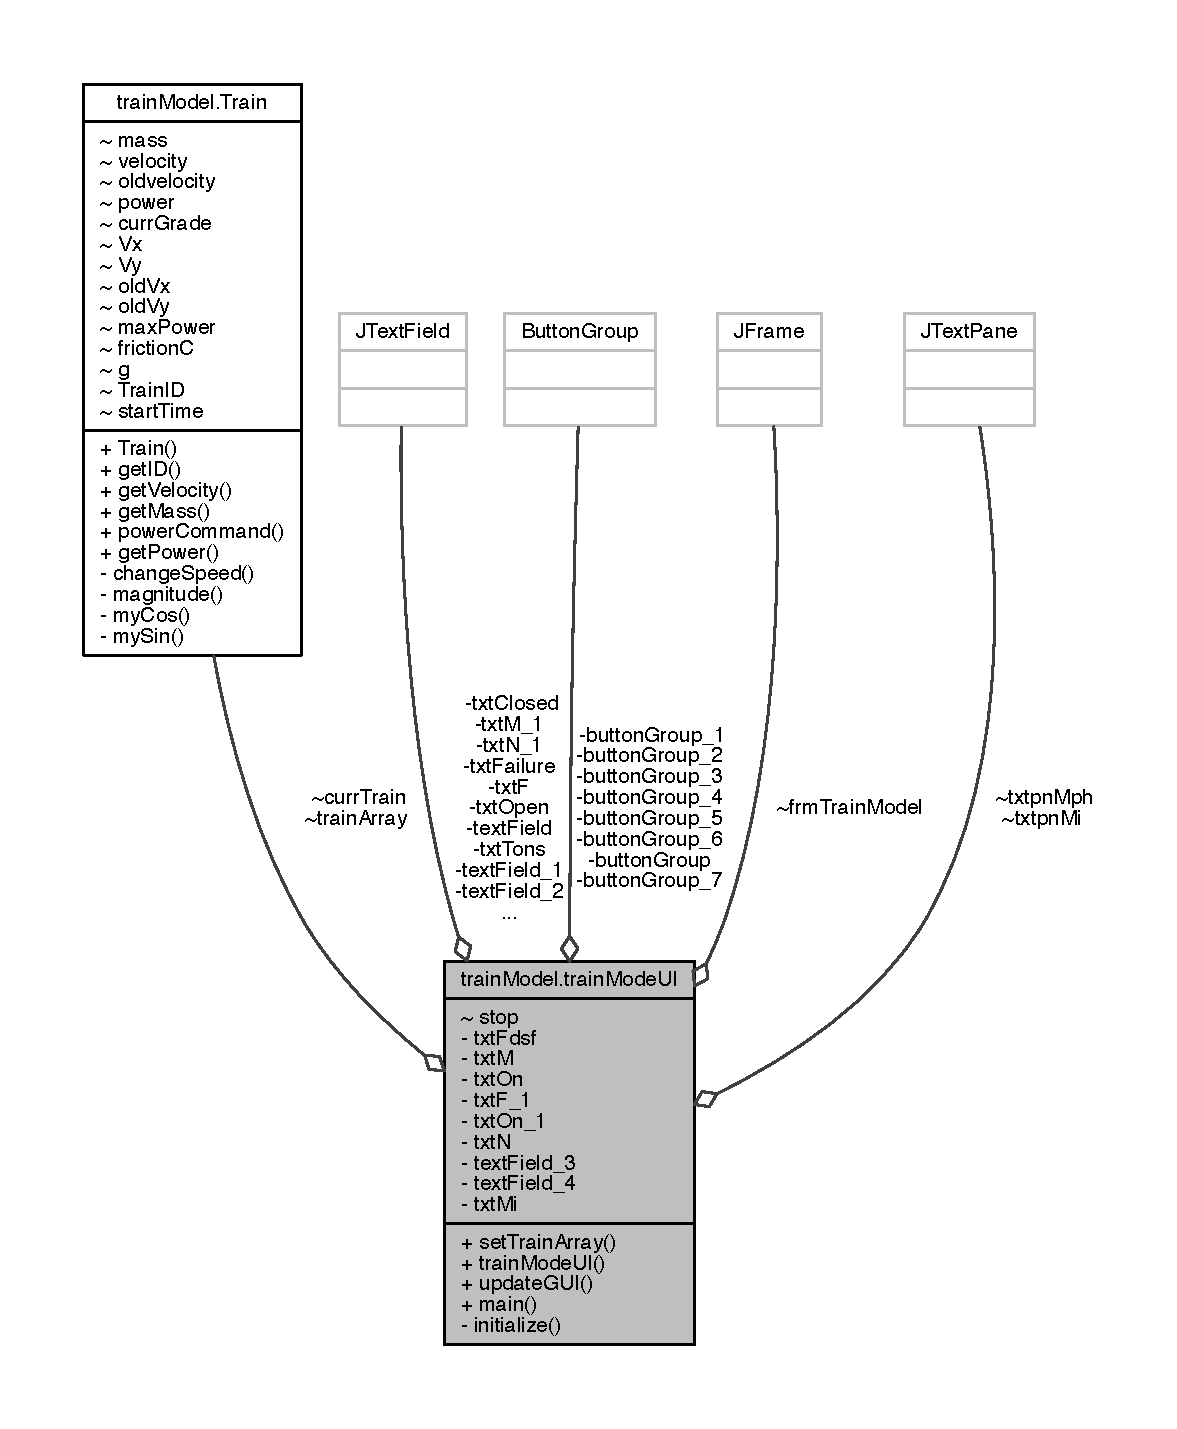
\includegraphics[width=350pt]{classtrainModel_1_1trainModeUI__coll__graph}
\end{center}
\end{figure}
\subsection*{Public Member Functions}
\begin{DoxyCompactItemize}
\item 
void \hyperlink{classtrainModel_1_1trainModeUI_a1d48455d0f924646325ee06eb4dd576d}{set\+Train\+Array} (\hyperlink{classtrainModel_1_1Train}{Train} \mbox{[}$\,$\mbox{]} trains)
\begin{DoxyCompactList}\small\item\em \hyperlink{classtrainModel_1_1Launch}{Launch} the application. \end{DoxyCompactList}\item 
\hyperlink{classtrainModel_1_1trainModeUI_adcb73bee7b6c10d7fce3a924b2fe092a}{train\+Mode\+UI} ()
\begin{DoxyCompactList}\small\item\em Create the application. \end{DoxyCompactList}\item 
void \hyperlink{classtrainModel_1_1trainModeUI_a1bb320064d891a9e4dfb26497f4c9d02}{update\+G\+UI} (\hyperlink{classtrainModel_1_1Train}{Train} currT)
\end{DoxyCompactItemize}
\subsection*{Static Public Member Functions}
\begin{DoxyCompactItemize}
\item 
static void \hyperlink{classtrainModel_1_1trainModeUI_a450d0a951e51bfe7f706c34275ba3e68}{main} (String\mbox{[}$\,$\mbox{]} args)
\end{DoxyCompactItemize}
\subsection*{Package Attributes}
\begin{DoxyCompactItemize}
\item 
J\+Frame \hyperlink{classtrainModel_1_1trainModeUI_ae35615a7c4b9acce2608935634929701}{frm\+Train\+Model}
\item 
J\+Text\+Pane \hyperlink{classtrainModel_1_1trainModeUI_ae4b47a5e7b1acac1da766e69c8bda376}{txtpn\+Mph}
\item 
J\+Text\+Pane \hyperlink{classtrainModel_1_1trainModeUI_ac47691c686814bf3314aca4a1519bedf}{txtpn\+Mi}
\item 
int \hyperlink{classtrainModel_1_1trainModeUI_a5d30f5361e1ed5891950e6d7690d4a58}{stop}
\end{DoxyCompactItemize}
\subsection*{Static Package Attributes}
\begin{DoxyCompactItemize}
\item 
static \hyperlink{classtrainModel_1_1Train}{Train} \mbox{[}$\,$\mbox{]} \hyperlink{classtrainModel_1_1trainModeUI_a5033486d5a74c3044a2c1bae958098aa}{train\+Array}
\item 
static \hyperlink{classtrainModel_1_1Train}{Train} \hyperlink{classtrainModel_1_1trainModeUI_aa9b65602131a0017c35ba3971d414793}{curr\+Train}
\end{DoxyCompactItemize}
\subsection*{Private Member Functions}
\begin{DoxyCompactItemize}
\item 
void \hyperlink{classtrainModel_1_1trainModeUI_a16cac97f7a09b9f1fbe5bf6a9c6909e8}{initialize} ()
\begin{DoxyCompactList}\small\item\em Initialize the contents of the frame. \end{DoxyCompactList}\end{DoxyCompactItemize}
\subsection*{Private Attributes}
\begin{DoxyCompactItemize}
\item 
J\+Text\+Field \hyperlink{classtrainModel_1_1trainModeUI_a20696c2664cf2d16d74fe7748ca27528}{txt\+Fdsf}
\item 
J\+Text\+Field \hyperlink{classtrainModel_1_1trainModeUI_a4f1c859e90a27f6311c07ee97ba967e6}{txtM}
\item 
J\+Text\+Field \hyperlink{classtrainModel_1_1trainModeUI_acd902e1db60c895f5be53727b0f248ee}{txt\+M\+\_\+1}
\item 
J\+Text\+Field \hyperlink{classtrainModel_1_1trainModeUI_a7a675397b2b4acb01241e1ce1374976d}{txt\+Tons}
\item 
J\+Text\+Field \hyperlink{classtrainModel_1_1trainModeUI_a3e9fdcb1083dfa4315b8dda29ee75042}{text\+Field}
\item 
J\+Text\+Field \hyperlink{classtrainModel_1_1trainModeUI_a857bc4073de2afc7380c4d0b964b4d9f}{text\+Field\+\_\+1}
\item 
J\+Text\+Field \hyperlink{classtrainModel_1_1trainModeUI_a640da80d6f928a8eb0fdbabee60889e1}{text\+Field\+\_\+2}
\item 
J\+Text\+Field \hyperlink{classtrainModel_1_1trainModeUI_a7ebf4529ce67fc221de9a471ba139eb1}{txt\+Open}
\item 
J\+Text\+Field \hyperlink{classtrainModel_1_1trainModeUI_aca941e25e51f32885348cf98ac64cc4e}{txt\+Closed}
\item 
J\+Text\+Field \hyperlink{classtrainModel_1_1trainModeUI_ab60f67f2cb49f6fe6856d516b0bda156}{txt\+On}
\item 
J\+Text\+Field \hyperlink{classtrainModel_1_1trainModeUI_a33c6151bdffc6fc460e5fb0f8b54ce3f}{txtF}
\item 
J\+Text\+Field \hyperlink{classtrainModel_1_1trainModeUI_adfd0ca58f1fdeea7894024f084f6024d}{txt\+F\+\_\+1}
\item 
J\+Text\+Field \hyperlink{classtrainModel_1_1trainModeUI_a44943cda5e52d523f428baefd0bea852}{txt\+Failure}
\item 
J\+Text\+Field \hyperlink{classtrainModel_1_1trainModeUI_a8fc05f34670a7a3e35bec5d14f3a34c1}{txt\+On\+\_\+1}
\item 
J\+Text\+Field \hyperlink{classtrainModel_1_1trainModeUI_aa84a6b1ee3e755def97e24e270b8b376}{txtN}
\item 
J\+Text\+Field \hyperlink{classtrainModel_1_1trainModeUI_ac528e4e64f0a0f0bb7d1ede997059b1a}{text\+Field\+\_\+3}
\item 
J\+Text\+Field \hyperlink{classtrainModel_1_1trainModeUI_a145ab9a2bcc199aa2f33f7d9bb0d84d6}{txt\+N\+\_\+1}
\item 
J\+Text\+Field \hyperlink{classtrainModel_1_1trainModeUI_a23053c176c8d26dfb31559c638873e12}{text\+Field\+\_\+4}
\item 
J\+Text\+Field \hyperlink{classtrainModel_1_1trainModeUI_a1705d34b28dc270079c8d965f2d64aab}{txt\+Mi}
\item 
final Button\+Group \hyperlink{classtrainModel_1_1trainModeUI_a51a47187c73fde59eab68c64be9659a2}{button\+Group} = new Button\+Group()
\item 
final Button\+Group \hyperlink{classtrainModel_1_1trainModeUI_a5bb8829ce826608235046acb2eaa2412}{button\+Group\+\_\+1} = new Button\+Group()
\item 
final Button\+Group \hyperlink{classtrainModel_1_1trainModeUI_a00aa346c55702462ecd81189215323dd}{button\+Group\+\_\+2} = new Button\+Group()
\item 
final Button\+Group \hyperlink{classtrainModel_1_1trainModeUI_a32bcd5e2a96960256ff54f3d102b733c}{button\+Group\+\_\+3} = new Button\+Group()
\item 
final Button\+Group \hyperlink{classtrainModel_1_1trainModeUI_a882be98e88b112093ba96d46c91ef28d}{button\+Group\+\_\+4} = new Button\+Group()
\item 
final Button\+Group \hyperlink{classtrainModel_1_1trainModeUI_a673b745ab85682f23ef1e47d314ae7e2}{button\+Group\+\_\+5} = new Button\+Group()
\item 
final Button\+Group \hyperlink{classtrainModel_1_1trainModeUI_a10b200816aff0e5040f44a619abe1230}{button\+Group\+\_\+6} = new Button\+Group()
\item 
final Button\+Group \hyperlink{classtrainModel_1_1trainModeUI_a6515fdd149165f9e0ddf31cfba57d211}{button\+Group\+\_\+7} = new Button\+Group()
\end{DoxyCompactItemize}


\subsection{Constructor \& Destructor Documentation}
\mbox{\Hypertarget{classtrainModel_1_1trainModeUI_adcb73bee7b6c10d7fce3a924b2fe092a}\label{classtrainModel_1_1trainModeUI_adcb73bee7b6c10d7fce3a924b2fe092a}} 
\index{train\+Model\+::train\+Mode\+UI@{train\+Model\+::train\+Mode\+UI}!train\+Mode\+UI@{train\+Mode\+UI}}
\index{train\+Mode\+UI@{train\+Mode\+UI}!train\+Model\+::train\+Mode\+UI@{train\+Model\+::train\+Mode\+UI}}
\subsubsection{\texorpdfstring{train\+Mode\+U\+I()}{trainModeUI()}}
{\footnotesize\ttfamily train\+Model.\+train\+Mode\+U\+I.\+train\+Mode\+UI (\begin{DoxyParamCaption}{ }\end{DoxyParamCaption})}



Create the application. 



\subsection{Member Function Documentation}
\mbox{\Hypertarget{classtrainModel_1_1trainModeUI_a16cac97f7a09b9f1fbe5bf6a9c6909e8}\label{classtrainModel_1_1trainModeUI_a16cac97f7a09b9f1fbe5bf6a9c6909e8}} 
\index{train\+Model\+::train\+Mode\+UI@{train\+Model\+::train\+Mode\+UI}!initialize@{initialize}}
\index{initialize@{initialize}!train\+Model\+::train\+Mode\+UI@{train\+Model\+::train\+Mode\+UI}}
\subsubsection{\texorpdfstring{initialize()}{initialize()}}
{\footnotesize\ttfamily void train\+Model.\+train\+Mode\+U\+I.\+initialize (\begin{DoxyParamCaption}{ }\end{DoxyParamCaption})\hspace{0.3cm}{\ttfamily [private]}}



Initialize the contents of the frame. 

\mbox{\Hypertarget{classtrainModel_1_1trainModeUI_a450d0a951e51bfe7f706c34275ba3e68}\label{classtrainModel_1_1trainModeUI_a450d0a951e51bfe7f706c34275ba3e68}} 
\index{train\+Model\+::train\+Mode\+UI@{train\+Model\+::train\+Mode\+UI}!main@{main}}
\index{main@{main}!train\+Model\+::train\+Mode\+UI@{train\+Model\+::train\+Mode\+UI}}
\subsubsection{\texorpdfstring{main()}{main()}}
{\footnotesize\ttfamily static void train\+Model.\+train\+Mode\+U\+I.\+main (\begin{DoxyParamCaption}\item[{String \mbox{[}$\,$\mbox{]}}]{args }\end{DoxyParamCaption})\hspace{0.3cm}{\ttfamily [static]}}

\mbox{\Hypertarget{classtrainModel_1_1trainModeUI_a1d48455d0f924646325ee06eb4dd576d}\label{classtrainModel_1_1trainModeUI_a1d48455d0f924646325ee06eb4dd576d}} 
\index{train\+Model\+::train\+Mode\+UI@{train\+Model\+::train\+Mode\+UI}!set\+Train\+Array@{set\+Train\+Array}}
\index{set\+Train\+Array@{set\+Train\+Array}!train\+Model\+::train\+Mode\+UI@{train\+Model\+::train\+Mode\+UI}}
\subsubsection{\texorpdfstring{set\+Train\+Array()}{setTrainArray()}}
{\footnotesize\ttfamily void train\+Model.\+train\+Mode\+U\+I.\+set\+Train\+Array (\begin{DoxyParamCaption}\item[{\hyperlink{classtrainModel_1_1Train}{Train} \mbox{[}$\,$\mbox{]}}]{trains }\end{DoxyParamCaption})}



\hyperlink{classtrainModel_1_1Launch}{Launch} the application. 


\begin{DoxyExceptions}{Exceptions}
{\em Unsupported\+Look\+And\+Feel\+Exception} & \\
\hline
{\em Illegal\+Access\+Exception} & \\
\hline
{\em Instantiation\+Exception} & \\
\hline
{\em Class\+Not\+Found\+Exception} & \\
\hline
\end{DoxyExceptions}
\mbox{\Hypertarget{classtrainModel_1_1trainModeUI_a1bb320064d891a9e4dfb26497f4c9d02}\label{classtrainModel_1_1trainModeUI_a1bb320064d891a9e4dfb26497f4c9d02}} 
\index{train\+Model\+::train\+Mode\+UI@{train\+Model\+::train\+Mode\+UI}!update\+G\+UI@{update\+G\+UI}}
\index{update\+G\+UI@{update\+G\+UI}!train\+Model\+::train\+Mode\+UI@{train\+Model\+::train\+Mode\+UI}}
\subsubsection{\texorpdfstring{update\+G\+U\+I()}{updateGUI()}}
{\footnotesize\ttfamily void train\+Model.\+train\+Mode\+U\+I.\+update\+G\+UI (\begin{DoxyParamCaption}\item[{\hyperlink{classtrainModel_1_1Train}{Train}}]{currT }\end{DoxyParamCaption})}



\subsection{Member Data Documentation}
\mbox{\Hypertarget{classtrainModel_1_1trainModeUI_a51a47187c73fde59eab68c64be9659a2}\label{classtrainModel_1_1trainModeUI_a51a47187c73fde59eab68c64be9659a2}} 
\index{train\+Model\+::train\+Mode\+UI@{train\+Model\+::train\+Mode\+UI}!button\+Group@{button\+Group}}
\index{button\+Group@{button\+Group}!train\+Model\+::train\+Mode\+UI@{train\+Model\+::train\+Mode\+UI}}
\subsubsection{\texorpdfstring{button\+Group}{buttonGroup}}
{\footnotesize\ttfamily final Button\+Group train\+Model.\+train\+Mode\+U\+I.\+button\+Group = new Button\+Group()\hspace{0.3cm}{\ttfamily [private]}}

\mbox{\Hypertarget{classtrainModel_1_1trainModeUI_a5bb8829ce826608235046acb2eaa2412}\label{classtrainModel_1_1trainModeUI_a5bb8829ce826608235046acb2eaa2412}} 
\index{train\+Model\+::train\+Mode\+UI@{train\+Model\+::train\+Mode\+UI}!button\+Group\+\_\+1@{button\+Group\+\_\+1}}
\index{button\+Group\+\_\+1@{button\+Group\+\_\+1}!train\+Model\+::train\+Mode\+UI@{train\+Model\+::train\+Mode\+UI}}
\subsubsection{\texorpdfstring{button\+Group\+\_\+1}{buttonGroup\_1}}
{\footnotesize\ttfamily final Button\+Group train\+Model.\+train\+Mode\+U\+I.\+button\+Group\+\_\+1 = new Button\+Group()\hspace{0.3cm}{\ttfamily [private]}}

\mbox{\Hypertarget{classtrainModel_1_1trainModeUI_a00aa346c55702462ecd81189215323dd}\label{classtrainModel_1_1trainModeUI_a00aa346c55702462ecd81189215323dd}} 
\index{train\+Model\+::train\+Mode\+UI@{train\+Model\+::train\+Mode\+UI}!button\+Group\+\_\+2@{button\+Group\+\_\+2}}
\index{button\+Group\+\_\+2@{button\+Group\+\_\+2}!train\+Model\+::train\+Mode\+UI@{train\+Model\+::train\+Mode\+UI}}
\subsubsection{\texorpdfstring{button\+Group\+\_\+2}{buttonGroup\_2}}
{\footnotesize\ttfamily final Button\+Group train\+Model.\+train\+Mode\+U\+I.\+button\+Group\+\_\+2 = new Button\+Group()\hspace{0.3cm}{\ttfamily [private]}}

\mbox{\Hypertarget{classtrainModel_1_1trainModeUI_a32bcd5e2a96960256ff54f3d102b733c}\label{classtrainModel_1_1trainModeUI_a32bcd5e2a96960256ff54f3d102b733c}} 
\index{train\+Model\+::train\+Mode\+UI@{train\+Model\+::train\+Mode\+UI}!button\+Group\+\_\+3@{button\+Group\+\_\+3}}
\index{button\+Group\+\_\+3@{button\+Group\+\_\+3}!train\+Model\+::train\+Mode\+UI@{train\+Model\+::train\+Mode\+UI}}
\subsubsection{\texorpdfstring{button\+Group\+\_\+3}{buttonGroup\_3}}
{\footnotesize\ttfamily final Button\+Group train\+Model.\+train\+Mode\+U\+I.\+button\+Group\+\_\+3 = new Button\+Group()\hspace{0.3cm}{\ttfamily [private]}}

\mbox{\Hypertarget{classtrainModel_1_1trainModeUI_a882be98e88b112093ba96d46c91ef28d}\label{classtrainModel_1_1trainModeUI_a882be98e88b112093ba96d46c91ef28d}} 
\index{train\+Model\+::train\+Mode\+UI@{train\+Model\+::train\+Mode\+UI}!button\+Group\+\_\+4@{button\+Group\+\_\+4}}
\index{button\+Group\+\_\+4@{button\+Group\+\_\+4}!train\+Model\+::train\+Mode\+UI@{train\+Model\+::train\+Mode\+UI}}
\subsubsection{\texorpdfstring{button\+Group\+\_\+4}{buttonGroup\_4}}
{\footnotesize\ttfamily final Button\+Group train\+Model.\+train\+Mode\+U\+I.\+button\+Group\+\_\+4 = new Button\+Group()\hspace{0.3cm}{\ttfamily [private]}}

\mbox{\Hypertarget{classtrainModel_1_1trainModeUI_a673b745ab85682f23ef1e47d314ae7e2}\label{classtrainModel_1_1trainModeUI_a673b745ab85682f23ef1e47d314ae7e2}} 
\index{train\+Model\+::train\+Mode\+UI@{train\+Model\+::train\+Mode\+UI}!button\+Group\+\_\+5@{button\+Group\+\_\+5}}
\index{button\+Group\+\_\+5@{button\+Group\+\_\+5}!train\+Model\+::train\+Mode\+UI@{train\+Model\+::train\+Mode\+UI}}
\subsubsection{\texorpdfstring{button\+Group\+\_\+5}{buttonGroup\_5}}
{\footnotesize\ttfamily final Button\+Group train\+Model.\+train\+Mode\+U\+I.\+button\+Group\+\_\+5 = new Button\+Group()\hspace{0.3cm}{\ttfamily [private]}}

\mbox{\Hypertarget{classtrainModel_1_1trainModeUI_a10b200816aff0e5040f44a619abe1230}\label{classtrainModel_1_1trainModeUI_a10b200816aff0e5040f44a619abe1230}} 
\index{train\+Model\+::train\+Mode\+UI@{train\+Model\+::train\+Mode\+UI}!button\+Group\+\_\+6@{button\+Group\+\_\+6}}
\index{button\+Group\+\_\+6@{button\+Group\+\_\+6}!train\+Model\+::train\+Mode\+UI@{train\+Model\+::train\+Mode\+UI}}
\subsubsection{\texorpdfstring{button\+Group\+\_\+6}{buttonGroup\_6}}
{\footnotesize\ttfamily final Button\+Group train\+Model.\+train\+Mode\+U\+I.\+button\+Group\+\_\+6 = new Button\+Group()\hspace{0.3cm}{\ttfamily [private]}}

\mbox{\Hypertarget{classtrainModel_1_1trainModeUI_a6515fdd149165f9e0ddf31cfba57d211}\label{classtrainModel_1_1trainModeUI_a6515fdd149165f9e0ddf31cfba57d211}} 
\index{train\+Model\+::train\+Mode\+UI@{train\+Model\+::train\+Mode\+UI}!button\+Group\+\_\+7@{button\+Group\+\_\+7}}
\index{button\+Group\+\_\+7@{button\+Group\+\_\+7}!train\+Model\+::train\+Mode\+UI@{train\+Model\+::train\+Mode\+UI}}
\subsubsection{\texorpdfstring{button\+Group\+\_\+7}{buttonGroup\_7}}
{\footnotesize\ttfamily final Button\+Group train\+Model.\+train\+Mode\+U\+I.\+button\+Group\+\_\+7 = new Button\+Group()\hspace{0.3cm}{\ttfamily [private]}}

\mbox{\Hypertarget{classtrainModel_1_1trainModeUI_aa9b65602131a0017c35ba3971d414793}\label{classtrainModel_1_1trainModeUI_aa9b65602131a0017c35ba3971d414793}} 
\index{train\+Model\+::train\+Mode\+UI@{train\+Model\+::train\+Mode\+UI}!curr\+Train@{curr\+Train}}
\index{curr\+Train@{curr\+Train}!train\+Model\+::train\+Mode\+UI@{train\+Model\+::train\+Mode\+UI}}
\subsubsection{\texorpdfstring{curr\+Train}{currTrain}}
{\footnotesize\ttfamily \hyperlink{classtrainModel_1_1Train}{Train} train\+Model.\+train\+Mode\+U\+I.\+curr\+Train\hspace{0.3cm}{\ttfamily [static]}, {\ttfamily [package]}}

\mbox{\Hypertarget{classtrainModel_1_1trainModeUI_ae35615a7c4b9acce2608935634929701}\label{classtrainModel_1_1trainModeUI_ae35615a7c4b9acce2608935634929701}} 
\index{train\+Model\+::train\+Mode\+UI@{train\+Model\+::train\+Mode\+UI}!frm\+Train\+Model@{frm\+Train\+Model}}
\index{frm\+Train\+Model@{frm\+Train\+Model}!train\+Model\+::train\+Mode\+UI@{train\+Model\+::train\+Mode\+UI}}
\subsubsection{\texorpdfstring{frm\+Train\+Model}{frmTrainModel}}
{\footnotesize\ttfamily J\+Frame train\+Model.\+train\+Mode\+U\+I.\+frm\+Train\+Model\hspace{0.3cm}{\ttfamily [package]}}

\mbox{\Hypertarget{classtrainModel_1_1trainModeUI_a5d30f5361e1ed5891950e6d7690d4a58}\label{classtrainModel_1_1trainModeUI_a5d30f5361e1ed5891950e6d7690d4a58}} 
\index{train\+Model\+::train\+Mode\+UI@{train\+Model\+::train\+Mode\+UI}!stop@{stop}}
\index{stop@{stop}!train\+Model\+::train\+Mode\+UI@{train\+Model\+::train\+Mode\+UI}}
\subsubsection{\texorpdfstring{stop}{stop}}
{\footnotesize\ttfamily int train\+Model.\+train\+Mode\+U\+I.\+stop\hspace{0.3cm}{\ttfamily [package]}}

\mbox{\Hypertarget{classtrainModel_1_1trainModeUI_a3e9fdcb1083dfa4315b8dda29ee75042}\label{classtrainModel_1_1trainModeUI_a3e9fdcb1083dfa4315b8dda29ee75042}} 
\index{train\+Model\+::train\+Mode\+UI@{train\+Model\+::train\+Mode\+UI}!text\+Field@{text\+Field}}
\index{text\+Field@{text\+Field}!train\+Model\+::train\+Mode\+UI@{train\+Model\+::train\+Mode\+UI}}
\subsubsection{\texorpdfstring{text\+Field}{textField}}
{\footnotesize\ttfamily J\+Text\+Field train\+Model.\+train\+Mode\+U\+I.\+text\+Field\hspace{0.3cm}{\ttfamily [private]}}

\mbox{\Hypertarget{classtrainModel_1_1trainModeUI_a857bc4073de2afc7380c4d0b964b4d9f}\label{classtrainModel_1_1trainModeUI_a857bc4073de2afc7380c4d0b964b4d9f}} 
\index{train\+Model\+::train\+Mode\+UI@{train\+Model\+::train\+Mode\+UI}!text\+Field\+\_\+1@{text\+Field\+\_\+1}}
\index{text\+Field\+\_\+1@{text\+Field\+\_\+1}!train\+Model\+::train\+Mode\+UI@{train\+Model\+::train\+Mode\+UI}}
\subsubsection{\texorpdfstring{text\+Field\+\_\+1}{textField\_1}}
{\footnotesize\ttfamily J\+Text\+Field train\+Model.\+train\+Mode\+U\+I.\+text\+Field\+\_\+1\hspace{0.3cm}{\ttfamily [private]}}

\mbox{\Hypertarget{classtrainModel_1_1trainModeUI_a640da80d6f928a8eb0fdbabee60889e1}\label{classtrainModel_1_1trainModeUI_a640da80d6f928a8eb0fdbabee60889e1}} 
\index{train\+Model\+::train\+Mode\+UI@{train\+Model\+::train\+Mode\+UI}!text\+Field\+\_\+2@{text\+Field\+\_\+2}}
\index{text\+Field\+\_\+2@{text\+Field\+\_\+2}!train\+Model\+::train\+Mode\+UI@{train\+Model\+::train\+Mode\+UI}}
\subsubsection{\texorpdfstring{text\+Field\+\_\+2}{textField\_2}}
{\footnotesize\ttfamily J\+Text\+Field train\+Model.\+train\+Mode\+U\+I.\+text\+Field\+\_\+2\hspace{0.3cm}{\ttfamily [private]}}

\mbox{\Hypertarget{classtrainModel_1_1trainModeUI_ac528e4e64f0a0f0bb7d1ede997059b1a}\label{classtrainModel_1_1trainModeUI_ac528e4e64f0a0f0bb7d1ede997059b1a}} 
\index{train\+Model\+::train\+Mode\+UI@{train\+Model\+::train\+Mode\+UI}!text\+Field\+\_\+3@{text\+Field\+\_\+3}}
\index{text\+Field\+\_\+3@{text\+Field\+\_\+3}!train\+Model\+::train\+Mode\+UI@{train\+Model\+::train\+Mode\+UI}}
\subsubsection{\texorpdfstring{text\+Field\+\_\+3}{textField\_3}}
{\footnotesize\ttfamily J\+Text\+Field train\+Model.\+train\+Mode\+U\+I.\+text\+Field\+\_\+3\hspace{0.3cm}{\ttfamily [private]}}

\mbox{\Hypertarget{classtrainModel_1_1trainModeUI_a23053c176c8d26dfb31559c638873e12}\label{classtrainModel_1_1trainModeUI_a23053c176c8d26dfb31559c638873e12}} 
\index{train\+Model\+::train\+Mode\+UI@{train\+Model\+::train\+Mode\+UI}!text\+Field\+\_\+4@{text\+Field\+\_\+4}}
\index{text\+Field\+\_\+4@{text\+Field\+\_\+4}!train\+Model\+::train\+Mode\+UI@{train\+Model\+::train\+Mode\+UI}}
\subsubsection{\texorpdfstring{text\+Field\+\_\+4}{textField\_4}}
{\footnotesize\ttfamily J\+Text\+Field train\+Model.\+train\+Mode\+U\+I.\+text\+Field\+\_\+4\hspace{0.3cm}{\ttfamily [private]}}

\mbox{\Hypertarget{classtrainModel_1_1trainModeUI_a5033486d5a74c3044a2c1bae958098aa}\label{classtrainModel_1_1trainModeUI_a5033486d5a74c3044a2c1bae958098aa}} 
\index{train\+Model\+::train\+Mode\+UI@{train\+Model\+::train\+Mode\+UI}!train\+Array@{train\+Array}}
\index{train\+Array@{train\+Array}!train\+Model\+::train\+Mode\+UI@{train\+Model\+::train\+Mode\+UI}}
\subsubsection{\texorpdfstring{train\+Array}{trainArray}}
{\footnotesize\ttfamily \hyperlink{classtrainModel_1_1Train}{Train} \mbox{[}$\,$\mbox{]} train\+Model.\+train\+Mode\+U\+I.\+train\+Array\hspace{0.3cm}{\ttfamily [static]}, {\ttfamily [package]}}

\mbox{\Hypertarget{classtrainModel_1_1trainModeUI_aca941e25e51f32885348cf98ac64cc4e}\label{classtrainModel_1_1trainModeUI_aca941e25e51f32885348cf98ac64cc4e}} 
\index{train\+Model\+::train\+Mode\+UI@{train\+Model\+::train\+Mode\+UI}!txt\+Closed@{txt\+Closed}}
\index{txt\+Closed@{txt\+Closed}!train\+Model\+::train\+Mode\+UI@{train\+Model\+::train\+Mode\+UI}}
\subsubsection{\texorpdfstring{txt\+Closed}{txtClosed}}
{\footnotesize\ttfamily J\+Text\+Field train\+Model.\+train\+Mode\+U\+I.\+txt\+Closed\hspace{0.3cm}{\ttfamily [private]}}

\mbox{\Hypertarget{classtrainModel_1_1trainModeUI_a33c6151bdffc6fc460e5fb0f8b54ce3f}\label{classtrainModel_1_1trainModeUI_a33c6151bdffc6fc460e5fb0f8b54ce3f}} 
\index{train\+Model\+::train\+Mode\+UI@{train\+Model\+::train\+Mode\+UI}!txtF@{txtF}}
\index{txtF@{txtF}!train\+Model\+::train\+Mode\+UI@{train\+Model\+::train\+Mode\+UI}}
\subsubsection{\texorpdfstring{txtF}{txtF}}
{\footnotesize\ttfamily J\+Text\+Field train\+Model.\+train\+Mode\+U\+I.\+txtF\hspace{0.3cm}{\ttfamily [private]}}

\mbox{\Hypertarget{classtrainModel_1_1trainModeUI_adfd0ca58f1fdeea7894024f084f6024d}\label{classtrainModel_1_1trainModeUI_adfd0ca58f1fdeea7894024f084f6024d}} 
\index{train\+Model\+::train\+Mode\+UI@{train\+Model\+::train\+Mode\+UI}!txt\+F\+\_\+1@{txt\+F\+\_\+1}}
\index{txt\+F\+\_\+1@{txt\+F\+\_\+1}!train\+Model\+::train\+Mode\+UI@{train\+Model\+::train\+Mode\+UI}}
\subsubsection{\texorpdfstring{txt\+F\+\_\+1}{txtF\_1}}
{\footnotesize\ttfamily J\+Text\+Field train\+Model.\+train\+Mode\+U\+I.\+txt\+F\+\_\+1\hspace{0.3cm}{\ttfamily [private]}}

\mbox{\Hypertarget{classtrainModel_1_1trainModeUI_a44943cda5e52d523f428baefd0bea852}\label{classtrainModel_1_1trainModeUI_a44943cda5e52d523f428baefd0bea852}} 
\index{train\+Model\+::train\+Mode\+UI@{train\+Model\+::train\+Mode\+UI}!txt\+Failure@{txt\+Failure}}
\index{txt\+Failure@{txt\+Failure}!train\+Model\+::train\+Mode\+UI@{train\+Model\+::train\+Mode\+UI}}
\subsubsection{\texorpdfstring{txt\+Failure}{txtFailure}}
{\footnotesize\ttfamily J\+Text\+Field train\+Model.\+train\+Mode\+U\+I.\+txt\+Failure\hspace{0.3cm}{\ttfamily [private]}}

\mbox{\Hypertarget{classtrainModel_1_1trainModeUI_a20696c2664cf2d16d74fe7748ca27528}\label{classtrainModel_1_1trainModeUI_a20696c2664cf2d16d74fe7748ca27528}} 
\index{train\+Model\+::train\+Mode\+UI@{train\+Model\+::train\+Mode\+UI}!txt\+Fdsf@{txt\+Fdsf}}
\index{txt\+Fdsf@{txt\+Fdsf}!train\+Model\+::train\+Mode\+UI@{train\+Model\+::train\+Mode\+UI}}
\subsubsection{\texorpdfstring{txt\+Fdsf}{txtFdsf}}
{\footnotesize\ttfamily J\+Text\+Field train\+Model.\+train\+Mode\+U\+I.\+txt\+Fdsf\hspace{0.3cm}{\ttfamily [private]}}

\mbox{\Hypertarget{classtrainModel_1_1trainModeUI_a4f1c859e90a27f6311c07ee97ba967e6}\label{classtrainModel_1_1trainModeUI_a4f1c859e90a27f6311c07ee97ba967e6}} 
\index{train\+Model\+::train\+Mode\+UI@{train\+Model\+::train\+Mode\+UI}!txtM@{txtM}}
\index{txtM@{txtM}!train\+Model\+::train\+Mode\+UI@{train\+Model\+::train\+Mode\+UI}}
\subsubsection{\texorpdfstring{txtM}{txtM}}
{\footnotesize\ttfamily J\+Text\+Field train\+Model.\+train\+Mode\+U\+I.\+txtM\hspace{0.3cm}{\ttfamily [private]}}

\mbox{\Hypertarget{classtrainModel_1_1trainModeUI_acd902e1db60c895f5be53727b0f248ee}\label{classtrainModel_1_1trainModeUI_acd902e1db60c895f5be53727b0f248ee}} 
\index{train\+Model\+::train\+Mode\+UI@{train\+Model\+::train\+Mode\+UI}!txt\+M\+\_\+1@{txt\+M\+\_\+1}}
\index{txt\+M\+\_\+1@{txt\+M\+\_\+1}!train\+Model\+::train\+Mode\+UI@{train\+Model\+::train\+Mode\+UI}}
\subsubsection{\texorpdfstring{txt\+M\+\_\+1}{txtM\_1}}
{\footnotesize\ttfamily J\+Text\+Field train\+Model.\+train\+Mode\+U\+I.\+txt\+M\+\_\+1\hspace{0.3cm}{\ttfamily [private]}}

\mbox{\Hypertarget{classtrainModel_1_1trainModeUI_a1705d34b28dc270079c8d965f2d64aab}\label{classtrainModel_1_1trainModeUI_a1705d34b28dc270079c8d965f2d64aab}} 
\index{train\+Model\+::train\+Mode\+UI@{train\+Model\+::train\+Mode\+UI}!txt\+Mi@{txt\+Mi}}
\index{txt\+Mi@{txt\+Mi}!train\+Model\+::train\+Mode\+UI@{train\+Model\+::train\+Mode\+UI}}
\subsubsection{\texorpdfstring{txt\+Mi}{txtMi}}
{\footnotesize\ttfamily J\+Text\+Field train\+Model.\+train\+Mode\+U\+I.\+txt\+Mi\hspace{0.3cm}{\ttfamily [private]}}

\mbox{\Hypertarget{classtrainModel_1_1trainModeUI_aa84a6b1ee3e755def97e24e270b8b376}\label{classtrainModel_1_1trainModeUI_aa84a6b1ee3e755def97e24e270b8b376}} 
\index{train\+Model\+::train\+Mode\+UI@{train\+Model\+::train\+Mode\+UI}!txtN@{txtN}}
\index{txtN@{txtN}!train\+Model\+::train\+Mode\+UI@{train\+Model\+::train\+Mode\+UI}}
\subsubsection{\texorpdfstring{txtN}{txtN}}
{\footnotesize\ttfamily J\+Text\+Field train\+Model.\+train\+Mode\+U\+I.\+txtN\hspace{0.3cm}{\ttfamily [private]}}

\mbox{\Hypertarget{classtrainModel_1_1trainModeUI_a145ab9a2bcc199aa2f33f7d9bb0d84d6}\label{classtrainModel_1_1trainModeUI_a145ab9a2bcc199aa2f33f7d9bb0d84d6}} 
\index{train\+Model\+::train\+Mode\+UI@{train\+Model\+::train\+Mode\+UI}!txt\+N\+\_\+1@{txt\+N\+\_\+1}}
\index{txt\+N\+\_\+1@{txt\+N\+\_\+1}!train\+Model\+::train\+Mode\+UI@{train\+Model\+::train\+Mode\+UI}}
\subsubsection{\texorpdfstring{txt\+N\+\_\+1}{txtN\_1}}
{\footnotesize\ttfamily J\+Text\+Field train\+Model.\+train\+Mode\+U\+I.\+txt\+N\+\_\+1\hspace{0.3cm}{\ttfamily [private]}}

\mbox{\Hypertarget{classtrainModel_1_1trainModeUI_ab60f67f2cb49f6fe6856d516b0bda156}\label{classtrainModel_1_1trainModeUI_ab60f67f2cb49f6fe6856d516b0bda156}} 
\index{train\+Model\+::train\+Mode\+UI@{train\+Model\+::train\+Mode\+UI}!txt\+On@{txt\+On}}
\index{txt\+On@{txt\+On}!train\+Model\+::train\+Mode\+UI@{train\+Model\+::train\+Mode\+UI}}
\subsubsection{\texorpdfstring{txt\+On}{txtOn}}
{\footnotesize\ttfamily J\+Text\+Field train\+Model.\+train\+Mode\+U\+I.\+txt\+On\hspace{0.3cm}{\ttfamily [private]}}

\mbox{\Hypertarget{classtrainModel_1_1trainModeUI_a8fc05f34670a7a3e35bec5d14f3a34c1}\label{classtrainModel_1_1trainModeUI_a8fc05f34670a7a3e35bec5d14f3a34c1}} 
\index{train\+Model\+::train\+Mode\+UI@{train\+Model\+::train\+Mode\+UI}!txt\+On\+\_\+1@{txt\+On\+\_\+1}}
\index{txt\+On\+\_\+1@{txt\+On\+\_\+1}!train\+Model\+::train\+Mode\+UI@{train\+Model\+::train\+Mode\+UI}}
\subsubsection{\texorpdfstring{txt\+On\+\_\+1}{txtOn\_1}}
{\footnotesize\ttfamily J\+Text\+Field train\+Model.\+train\+Mode\+U\+I.\+txt\+On\+\_\+1\hspace{0.3cm}{\ttfamily [private]}}

\mbox{\Hypertarget{classtrainModel_1_1trainModeUI_a7ebf4529ce67fc221de9a471ba139eb1}\label{classtrainModel_1_1trainModeUI_a7ebf4529ce67fc221de9a471ba139eb1}} 
\index{train\+Model\+::train\+Mode\+UI@{train\+Model\+::train\+Mode\+UI}!txt\+Open@{txt\+Open}}
\index{txt\+Open@{txt\+Open}!train\+Model\+::train\+Mode\+UI@{train\+Model\+::train\+Mode\+UI}}
\subsubsection{\texorpdfstring{txt\+Open}{txtOpen}}
{\footnotesize\ttfamily J\+Text\+Field train\+Model.\+train\+Mode\+U\+I.\+txt\+Open\hspace{0.3cm}{\ttfamily [private]}}

\mbox{\Hypertarget{classtrainModel_1_1trainModeUI_ac47691c686814bf3314aca4a1519bedf}\label{classtrainModel_1_1trainModeUI_ac47691c686814bf3314aca4a1519bedf}} 
\index{train\+Model\+::train\+Mode\+UI@{train\+Model\+::train\+Mode\+UI}!txtpn\+Mi@{txtpn\+Mi}}
\index{txtpn\+Mi@{txtpn\+Mi}!train\+Model\+::train\+Mode\+UI@{train\+Model\+::train\+Mode\+UI}}
\subsubsection{\texorpdfstring{txtpn\+Mi}{txtpnMi}}
{\footnotesize\ttfamily J\+Text\+Pane train\+Model.\+train\+Mode\+U\+I.\+txtpn\+Mi\hspace{0.3cm}{\ttfamily [package]}}

\mbox{\Hypertarget{classtrainModel_1_1trainModeUI_ae4b47a5e7b1acac1da766e69c8bda376}\label{classtrainModel_1_1trainModeUI_ae4b47a5e7b1acac1da766e69c8bda376}} 
\index{train\+Model\+::train\+Mode\+UI@{train\+Model\+::train\+Mode\+UI}!txtpn\+Mph@{txtpn\+Mph}}
\index{txtpn\+Mph@{txtpn\+Mph}!train\+Model\+::train\+Mode\+UI@{train\+Model\+::train\+Mode\+UI}}
\subsubsection{\texorpdfstring{txtpn\+Mph}{txtpnMph}}
{\footnotesize\ttfamily J\+Text\+Pane train\+Model.\+train\+Mode\+U\+I.\+txtpn\+Mph\hspace{0.3cm}{\ttfamily [package]}}

\mbox{\Hypertarget{classtrainModel_1_1trainModeUI_a7a675397b2b4acb01241e1ce1374976d}\label{classtrainModel_1_1trainModeUI_a7a675397b2b4acb01241e1ce1374976d}} 
\index{train\+Model\+::train\+Mode\+UI@{train\+Model\+::train\+Mode\+UI}!txt\+Tons@{txt\+Tons}}
\index{txt\+Tons@{txt\+Tons}!train\+Model\+::train\+Mode\+UI@{train\+Model\+::train\+Mode\+UI}}
\subsubsection{\texorpdfstring{txt\+Tons}{txtTons}}
{\footnotesize\ttfamily J\+Text\+Field train\+Model.\+train\+Mode\+U\+I.\+txt\+Tons\hspace{0.3cm}{\ttfamily [private]}}



The documentation for this class was generated from the following file\+:\begin{DoxyCompactItemize}
\item 
src/main/java/train\+Model/\hyperlink{trainModeUI_8java}{train\+Mode\+U\+I.\+java}\end{DoxyCompactItemize}

\hypertarget{classWaysideController_1_1WaysideGuiMain}{}\section{Wayside\+Controller.\+Wayside\+Gui\+Main Class Reference}
\label{classWaysideController_1_1WaysideGuiMain}\index{Wayside\+Controller.\+Wayside\+Gui\+Main@{Wayside\+Controller.\+Wayside\+Gui\+Main}}


Collaboration diagram for Wayside\+Controller.\+Wayside\+Gui\+Main\+:
\nopagebreak
\begin{figure}[H]
\begin{center}
\leavevmode
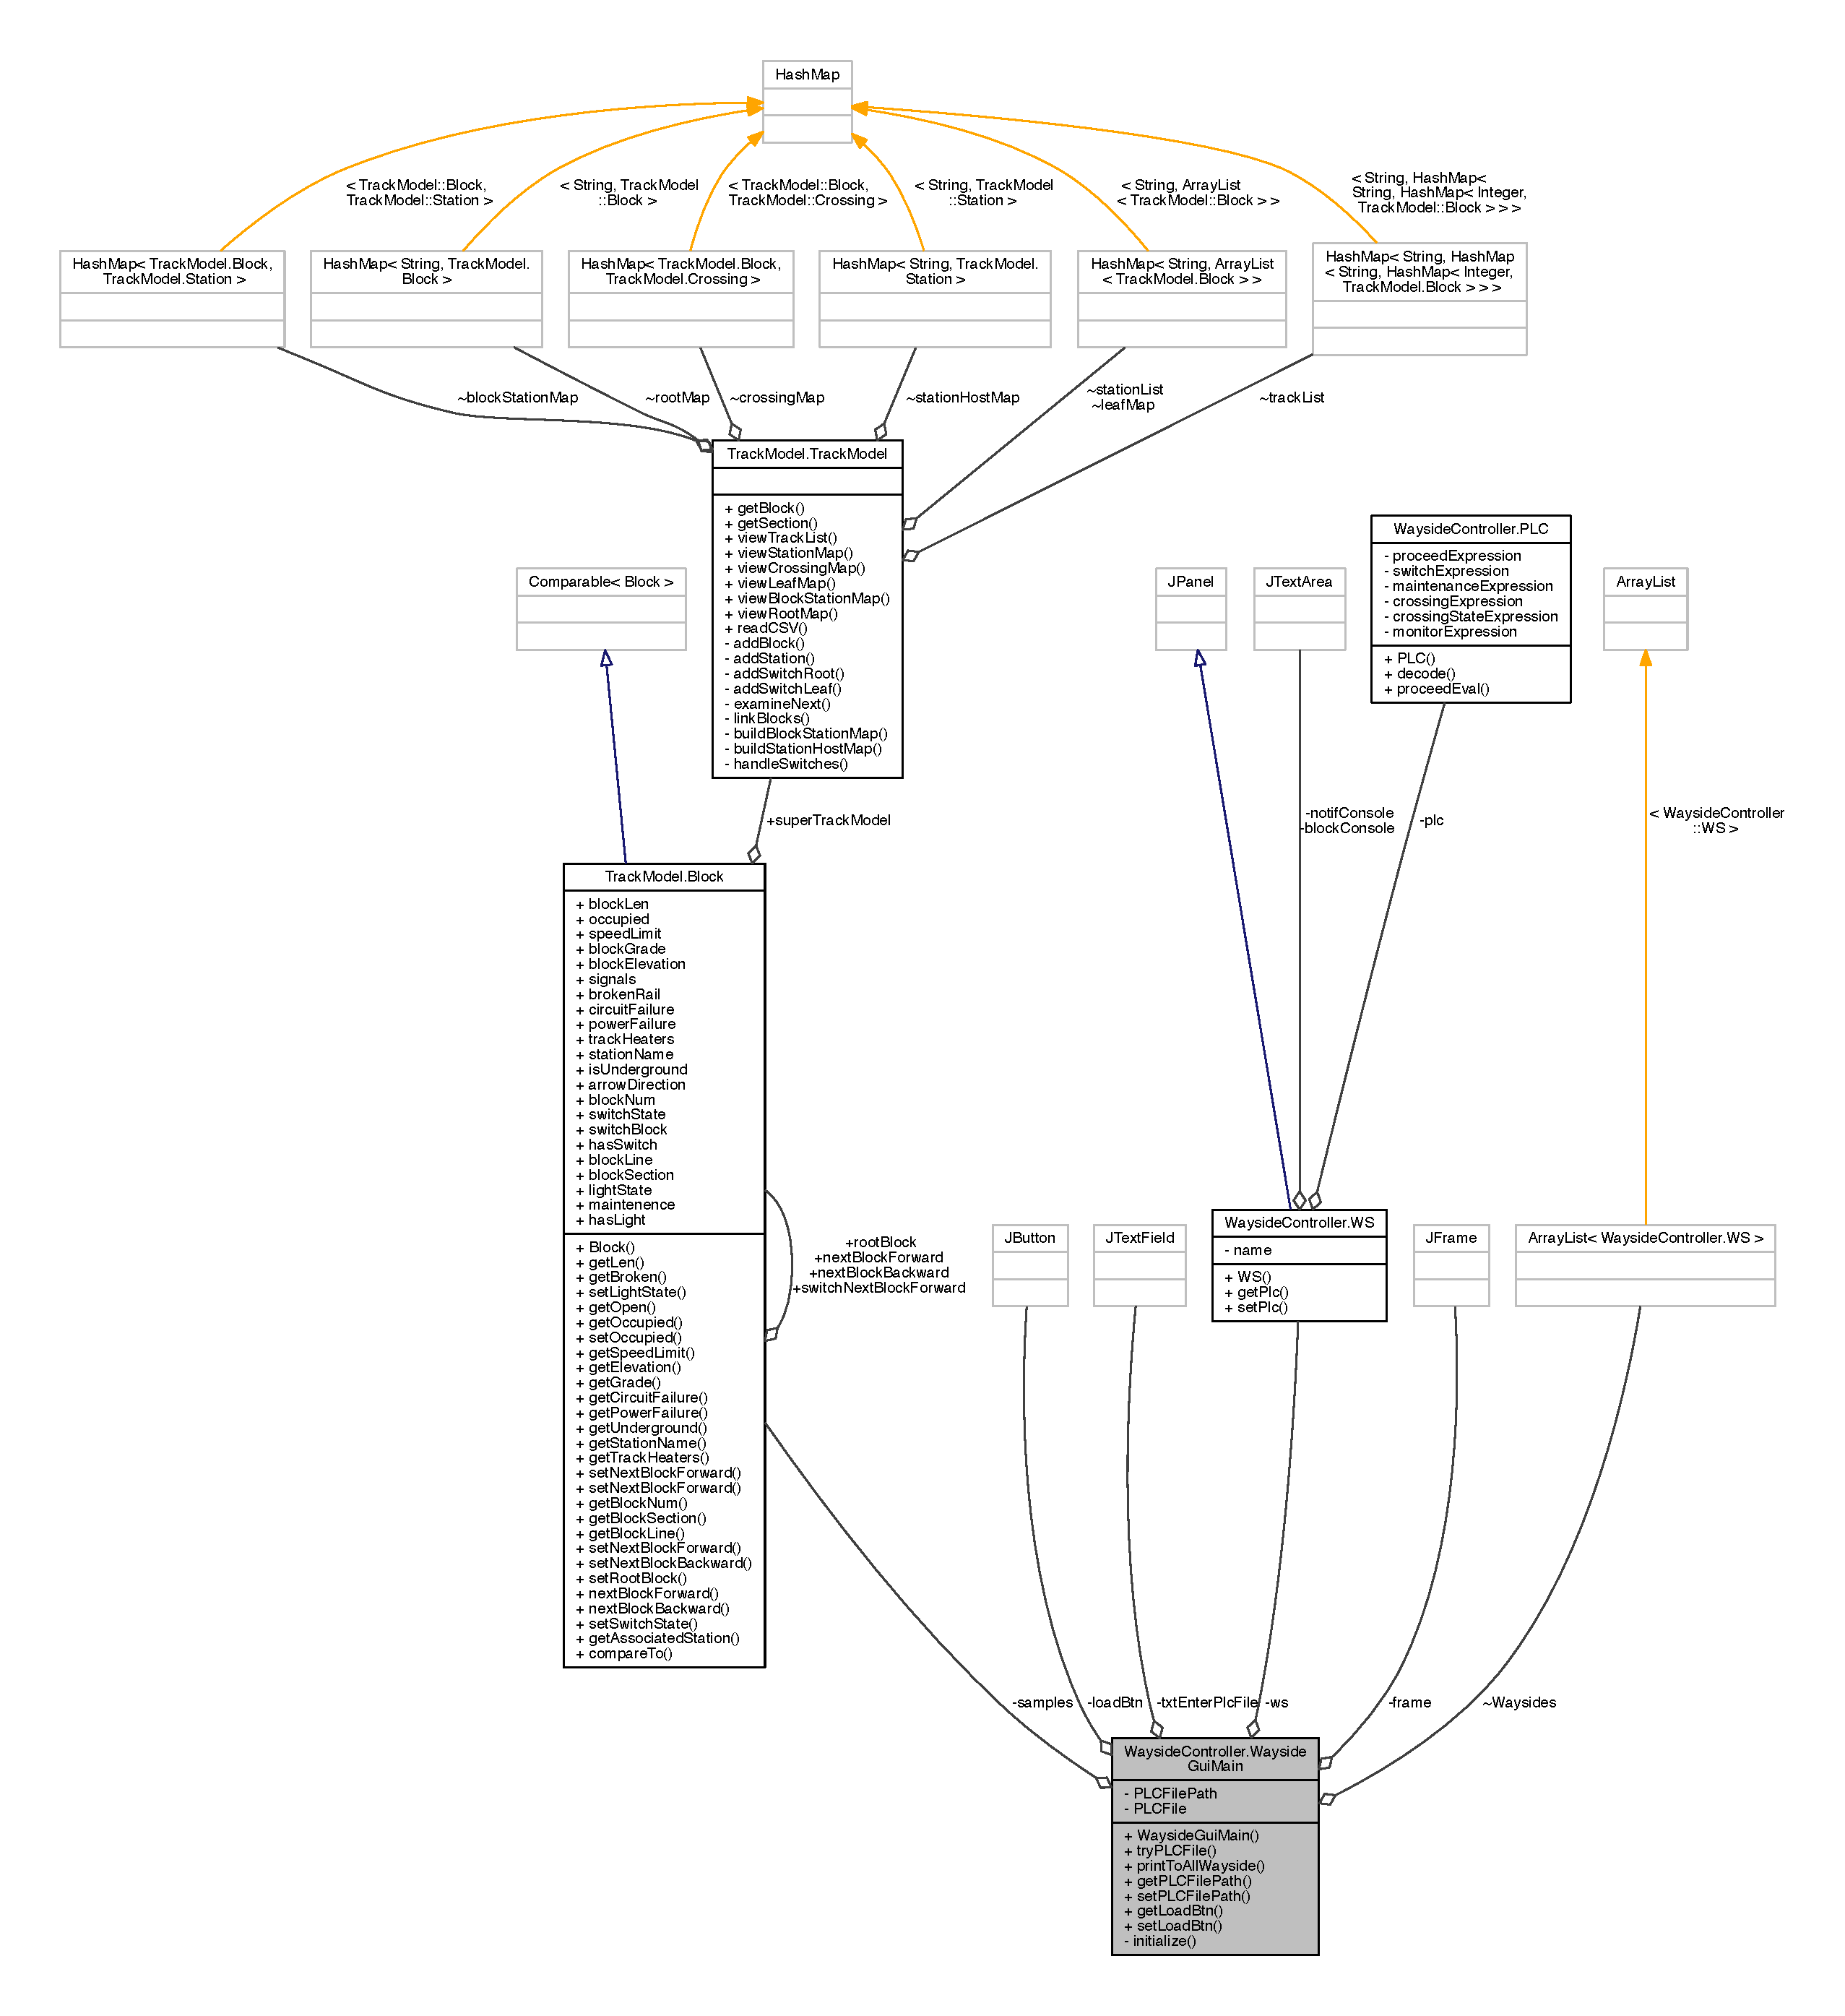
\includegraphics[width=350pt]{classWaysideController_1_1WaysideGuiMain__coll__graph}
\end{center}
\end{figure}
\subsection*{Public Member Functions}
\begin{DoxyCompactItemize}
\item 
\hyperlink{classWaysideController_1_1WaysideGuiMain_af5c9eea089aa061d0f027ccd27a458db}{Wayside\+Gui\+Main} (\hyperlink{classTrackModel_1_1TrackModel}{Track\+Model} track)  throws Class\+Not\+Found\+Exception, Instantiation\+Exception, Illegal\+Access\+Exception, Unsupported\+Look\+And\+Feel\+Exception, I\+O\+Exception 
\begin{DoxyCompactList}\small\item\em Launch the application. \end{DoxyCompactList}\item 
void \hyperlink{classWaysideController_1_1WaysideGuiMain_a5f4353da24b4d0f25ba614c69f8d37bd}{try\+P\+L\+C\+File} (String filename)  throws I\+O\+Exception, Script\+Exception
\begin{DoxyCompactList}\small\item\em Tries to open give \hyperlink{classWaysideController_1_1PLC}{P\+LC} file and checks for existence. \end{DoxyCompactList}\item 
void \hyperlink{classWaysideController_1_1WaysideGuiMain_aa1fb5c7338ec4b6840f45af2bc507712}{print\+To\+All\+Wayside} (String to\+Print)
\item 
String \hyperlink{classWaysideController_1_1WaysideGuiMain_aab8b7369a64aa177fabe7bbe4e1208ca}{get\+P\+L\+C\+File\+Path} ()
\item 
void \hyperlink{classWaysideController_1_1WaysideGuiMain_a15eb954941c4b70ea6a4b842a73781bf}{set\+P\+L\+C\+File\+Path} (String p\+L\+C\+File\+Path)
\item 
J\+Button \hyperlink{classWaysideController_1_1WaysideGuiMain_abdc61ffc03ce5e58bfa37142c1935677}{get\+Load\+Btn} ()
\item 
void \hyperlink{classWaysideController_1_1WaysideGuiMain_a46c43048836307c70180dfd30fceea79}{set\+Load\+Btn} (J\+Button \hyperlink{classWaysideController_1_1WaysideGuiMain_a6024b79350afc61454bea1574e16701d}{load\+Btn})
\end{DoxyCompactItemize}
\subsection*{Package Attributes}
\begin{DoxyCompactItemize}
\item 
Array\+List$<$ \hyperlink{classWaysideController_1_1WS}{WS} $>$ \hyperlink{classWaysideController_1_1WaysideGuiMain_afaf467ad6f10a2ad0601b35302aa684f}{Waysides} = new Array\+List$<$\hyperlink{classWaysideController_1_1WS}{WS}$>$()
\end{DoxyCompactItemize}
\subsection*{Private Member Functions}
\begin{DoxyCompactItemize}
\item 
void \hyperlink{classWaysideController_1_1WaysideGuiMain_a6f96f3a1fdd7cf7a05c281be97387413}{initialize} (\hyperlink{classTrackModel_1_1TrackModel}{Track\+Model} track)  throws Class\+Not\+Found\+Exception, Instantiation\+Exception, Illegal\+Access\+Exception, Unsupported\+Look\+And\+Feel\+Exception, I\+O\+Exception 
\begin{DoxyCompactList}\small\item\em Initialize the contents of the frame. \end{DoxyCompactList}\end{DoxyCompactItemize}
\subsection*{Private Attributes}
\begin{DoxyCompactItemize}
\item 
J\+Frame \hyperlink{classWaysideController_1_1WaysideGuiMain_a7bb363eb04328d1213e193d5710462c9}{frame}
\item 
J\+Text\+Field \hyperlink{classWaysideController_1_1WaysideGuiMain_a1fc195348c67f797d2319ef0ae9e7e21}{txt\+Enter\+Plc\+File}
\item 
String \hyperlink{classWaysideController_1_1WaysideGuiMain_a09e20ab379be966f13ef09a488b0d582}{P\+L\+C\+File\+Path}
\item 
J\+Button \hyperlink{classWaysideController_1_1WaysideGuiMain_a6024b79350afc61454bea1574e16701d}{load\+Btn}
\item 
File \hyperlink{classWaysideController_1_1WaysideGuiMain_a2971e6ce2f729012928bdbf69caf7ab2}{P\+L\+C\+File}
\item 
\hyperlink{classTrackModel_1_1Block}{Block} \mbox{[}$\,$\mbox{]} \hyperlink{classWaysideController_1_1WaysideGuiMain_ad43fe7fd3d059b7f994c52e90d72fb68}{samples}
\item 
\hyperlink{classWaysideController_1_1WS}{WS} \hyperlink{classWaysideController_1_1WaysideGuiMain_a10516fa6d5db77d5935135af8b0446c9}{ws}
\end{DoxyCompactItemize}


\subsection{Constructor \& Destructor Documentation}
\mbox{\Hypertarget{classWaysideController_1_1WaysideGuiMain_af5c9eea089aa061d0f027ccd27a458db}\label{classWaysideController_1_1WaysideGuiMain_af5c9eea089aa061d0f027ccd27a458db}} 
\index{Wayside\+Controller\+::\+Wayside\+Gui\+Main@{Wayside\+Controller\+::\+Wayside\+Gui\+Main}!Wayside\+Gui\+Main@{Wayside\+Gui\+Main}}
\index{Wayside\+Gui\+Main@{Wayside\+Gui\+Main}!Wayside\+Controller\+::\+Wayside\+Gui\+Main@{Wayside\+Controller\+::\+Wayside\+Gui\+Main}}
\subsubsection{\texorpdfstring{Wayside\+Gui\+Main()}{WaysideGuiMain()}}
{\footnotesize\ttfamily Wayside\+Controller.\+Wayside\+Gui\+Main.\+Wayside\+Gui\+Main (\begin{DoxyParamCaption}\item[{\hyperlink{classTrackModel_1_1TrackModel}{Track\+Model}}]{track }\end{DoxyParamCaption}) throws Class\+Not\+Found\+Exception, Instantiation\+Exception, Illegal\+Access\+Exception, Unsupported\+Look\+And\+Feel\+Exception, I\+O\+Exception}



Launch the application. 


\begin{DoxyExceptions}{Exceptions}
{\em Unsupported\+Look\+And\+Feel\+Exception} & \\
\hline
{\em Illegal\+Access\+Exception} & \\
\hline
{\em Instantiation\+Exception} & \\
\hline
{\em Class\+Not\+Found\+Exception} & Create the application. \\
\hline
{\em Unsupported\+Look\+And\+Feel\+Exception} & \\
\hline
{\em Illegal\+Access\+Exception} & \\
\hline
{\em Instantiation\+Exception} & \\
\hline
{\em Class\+Not\+Found\+Exception} & \\
\hline
{\em I\+O\+Exception} & \\
\hline
\end{DoxyExceptions}


\subsection{Member Function Documentation}
\mbox{\Hypertarget{classWaysideController_1_1WaysideGuiMain_abdc61ffc03ce5e58bfa37142c1935677}\label{classWaysideController_1_1WaysideGuiMain_abdc61ffc03ce5e58bfa37142c1935677}} 
\index{Wayside\+Controller\+::\+Wayside\+Gui\+Main@{Wayside\+Controller\+::\+Wayside\+Gui\+Main}!get\+Load\+Btn@{get\+Load\+Btn}}
\index{get\+Load\+Btn@{get\+Load\+Btn}!Wayside\+Controller\+::\+Wayside\+Gui\+Main@{Wayside\+Controller\+::\+Wayside\+Gui\+Main}}
\subsubsection{\texorpdfstring{get\+Load\+Btn()}{getLoadBtn()}}
{\footnotesize\ttfamily J\+Button Wayside\+Controller.\+Wayside\+Gui\+Main.\+get\+Load\+Btn (\begin{DoxyParamCaption}{ }\end{DoxyParamCaption})}

\mbox{\Hypertarget{classWaysideController_1_1WaysideGuiMain_aab8b7369a64aa177fabe7bbe4e1208ca}\label{classWaysideController_1_1WaysideGuiMain_aab8b7369a64aa177fabe7bbe4e1208ca}} 
\index{Wayside\+Controller\+::\+Wayside\+Gui\+Main@{Wayside\+Controller\+::\+Wayside\+Gui\+Main}!get\+P\+L\+C\+File\+Path@{get\+P\+L\+C\+File\+Path}}
\index{get\+P\+L\+C\+File\+Path@{get\+P\+L\+C\+File\+Path}!Wayside\+Controller\+::\+Wayside\+Gui\+Main@{Wayside\+Controller\+::\+Wayside\+Gui\+Main}}
\subsubsection{\texorpdfstring{get\+P\+L\+C\+File\+Path()}{getPLCFilePath()}}
{\footnotesize\ttfamily String Wayside\+Controller.\+Wayside\+Gui\+Main.\+get\+P\+L\+C\+File\+Path (\begin{DoxyParamCaption}{ }\end{DoxyParamCaption})}

\mbox{\Hypertarget{classWaysideController_1_1WaysideGuiMain_a6f96f3a1fdd7cf7a05c281be97387413}\label{classWaysideController_1_1WaysideGuiMain_a6f96f3a1fdd7cf7a05c281be97387413}} 
\index{Wayside\+Controller\+::\+Wayside\+Gui\+Main@{Wayside\+Controller\+::\+Wayside\+Gui\+Main}!initialize@{initialize}}
\index{initialize@{initialize}!Wayside\+Controller\+::\+Wayside\+Gui\+Main@{Wayside\+Controller\+::\+Wayside\+Gui\+Main}}
\subsubsection{\texorpdfstring{initialize()}{initialize()}}
{\footnotesize\ttfamily void Wayside\+Controller.\+Wayside\+Gui\+Main.\+initialize (\begin{DoxyParamCaption}\item[{\hyperlink{classTrackModel_1_1TrackModel}{Track\+Model}}]{track }\end{DoxyParamCaption}) throws Class\+Not\+Found\+Exception, Instantiation\+Exception, Illegal\+Access\+Exception, Unsupported\+Look\+And\+Feel\+Exception, I\+O\+Exception\hspace{0.3cm}{\ttfamily [private]}}



Initialize the contents of the frame. 


\begin{DoxyExceptions}{Exceptions}
{\em Unsupported\+Look\+And\+Feel\+Exception} & \\
\hline
{\em Illegal\+Access\+Exception} & \\
\hline
{\em Instantiation\+Exception} & \\
\hline
{\em Class\+Not\+Found\+Exception} & \\
\hline
{\em I\+O\+Exception} & \\
\hline
\end{DoxyExceptions}
\mbox{\Hypertarget{classWaysideController_1_1WaysideGuiMain_aa1fb5c7338ec4b6840f45af2bc507712}\label{classWaysideController_1_1WaysideGuiMain_aa1fb5c7338ec4b6840f45af2bc507712}} 
\index{Wayside\+Controller\+::\+Wayside\+Gui\+Main@{Wayside\+Controller\+::\+Wayside\+Gui\+Main}!print\+To\+All\+Wayside@{print\+To\+All\+Wayside}}
\index{print\+To\+All\+Wayside@{print\+To\+All\+Wayside}!Wayside\+Controller\+::\+Wayside\+Gui\+Main@{Wayside\+Controller\+::\+Wayside\+Gui\+Main}}
\subsubsection{\texorpdfstring{print\+To\+All\+Wayside()}{printToAllWayside()}}
{\footnotesize\ttfamily void Wayside\+Controller.\+Wayside\+Gui\+Main.\+print\+To\+All\+Wayside (\begin{DoxyParamCaption}\item[{String}]{to\+Print }\end{DoxyParamCaption})}

\mbox{\Hypertarget{classWaysideController_1_1WaysideGuiMain_a46c43048836307c70180dfd30fceea79}\label{classWaysideController_1_1WaysideGuiMain_a46c43048836307c70180dfd30fceea79}} 
\index{Wayside\+Controller\+::\+Wayside\+Gui\+Main@{Wayside\+Controller\+::\+Wayside\+Gui\+Main}!set\+Load\+Btn@{set\+Load\+Btn}}
\index{set\+Load\+Btn@{set\+Load\+Btn}!Wayside\+Controller\+::\+Wayside\+Gui\+Main@{Wayside\+Controller\+::\+Wayside\+Gui\+Main}}
\subsubsection{\texorpdfstring{set\+Load\+Btn()}{setLoadBtn()}}
{\footnotesize\ttfamily void Wayside\+Controller.\+Wayside\+Gui\+Main.\+set\+Load\+Btn (\begin{DoxyParamCaption}\item[{J\+Button}]{load\+Btn }\end{DoxyParamCaption})}

\mbox{\Hypertarget{classWaysideController_1_1WaysideGuiMain_a15eb954941c4b70ea6a4b842a73781bf}\label{classWaysideController_1_1WaysideGuiMain_a15eb954941c4b70ea6a4b842a73781bf}} 
\index{Wayside\+Controller\+::\+Wayside\+Gui\+Main@{Wayside\+Controller\+::\+Wayside\+Gui\+Main}!set\+P\+L\+C\+File\+Path@{set\+P\+L\+C\+File\+Path}}
\index{set\+P\+L\+C\+File\+Path@{set\+P\+L\+C\+File\+Path}!Wayside\+Controller\+::\+Wayside\+Gui\+Main@{Wayside\+Controller\+::\+Wayside\+Gui\+Main}}
\subsubsection{\texorpdfstring{set\+P\+L\+C\+File\+Path()}{setPLCFilePath()}}
{\footnotesize\ttfamily void Wayside\+Controller.\+Wayside\+Gui\+Main.\+set\+P\+L\+C\+File\+Path (\begin{DoxyParamCaption}\item[{String}]{p\+L\+C\+File\+Path }\end{DoxyParamCaption})}

\mbox{\Hypertarget{classWaysideController_1_1WaysideGuiMain_a5f4353da24b4d0f25ba614c69f8d37bd}\label{classWaysideController_1_1WaysideGuiMain_a5f4353da24b4d0f25ba614c69f8d37bd}} 
\index{Wayside\+Controller\+::\+Wayside\+Gui\+Main@{Wayside\+Controller\+::\+Wayside\+Gui\+Main}!try\+P\+L\+C\+File@{try\+P\+L\+C\+File}}
\index{try\+P\+L\+C\+File@{try\+P\+L\+C\+File}!Wayside\+Controller\+::\+Wayside\+Gui\+Main@{Wayside\+Controller\+::\+Wayside\+Gui\+Main}}
\subsubsection{\texorpdfstring{try\+P\+L\+C\+File()}{tryPLCFile()}}
{\footnotesize\ttfamily void Wayside\+Controller.\+Wayside\+Gui\+Main.\+try\+P\+L\+C\+File (\begin{DoxyParamCaption}\item[{String}]{filename }\end{DoxyParamCaption}) throws I\+O\+Exception, Script\+Exception}



Tries to open give \hyperlink{classWaysideController_1_1PLC}{P\+LC} file and checks for existence. 


\begin{DoxyParams}{Parameters}
{\em filename} & -\/ user entered filename/path of \hyperlink{classWaysideController_1_1PLC}{P\+LC} Code File \\
\hline
\end{DoxyParams}

\begin{DoxyExceptions}{Exceptions}
{\em I\+O\+Exception} & \\
\hline
{\em Script\+Exception} & \\
\hline
\end{DoxyExceptions}


\subsection{Member Data Documentation}
\mbox{\Hypertarget{classWaysideController_1_1WaysideGuiMain_a7bb363eb04328d1213e193d5710462c9}\label{classWaysideController_1_1WaysideGuiMain_a7bb363eb04328d1213e193d5710462c9}} 
\index{Wayside\+Controller\+::\+Wayside\+Gui\+Main@{Wayside\+Controller\+::\+Wayside\+Gui\+Main}!frame@{frame}}
\index{frame@{frame}!Wayside\+Controller\+::\+Wayside\+Gui\+Main@{Wayside\+Controller\+::\+Wayside\+Gui\+Main}}
\subsubsection{\texorpdfstring{frame}{frame}}
{\footnotesize\ttfamily J\+Frame Wayside\+Controller.\+Wayside\+Gui\+Main.\+frame\hspace{0.3cm}{\ttfamily [private]}}

\mbox{\Hypertarget{classWaysideController_1_1WaysideGuiMain_a6024b79350afc61454bea1574e16701d}\label{classWaysideController_1_1WaysideGuiMain_a6024b79350afc61454bea1574e16701d}} 
\index{Wayside\+Controller\+::\+Wayside\+Gui\+Main@{Wayside\+Controller\+::\+Wayside\+Gui\+Main}!load\+Btn@{load\+Btn}}
\index{load\+Btn@{load\+Btn}!Wayside\+Controller\+::\+Wayside\+Gui\+Main@{Wayside\+Controller\+::\+Wayside\+Gui\+Main}}
\subsubsection{\texorpdfstring{load\+Btn}{loadBtn}}
{\footnotesize\ttfamily J\+Button Wayside\+Controller.\+Wayside\+Gui\+Main.\+load\+Btn\hspace{0.3cm}{\ttfamily [private]}}

\mbox{\Hypertarget{classWaysideController_1_1WaysideGuiMain_a2971e6ce2f729012928bdbf69caf7ab2}\label{classWaysideController_1_1WaysideGuiMain_a2971e6ce2f729012928bdbf69caf7ab2}} 
\index{Wayside\+Controller\+::\+Wayside\+Gui\+Main@{Wayside\+Controller\+::\+Wayside\+Gui\+Main}!P\+L\+C\+File@{P\+L\+C\+File}}
\index{P\+L\+C\+File@{P\+L\+C\+File}!Wayside\+Controller\+::\+Wayside\+Gui\+Main@{Wayside\+Controller\+::\+Wayside\+Gui\+Main}}
\subsubsection{\texorpdfstring{P\+L\+C\+File}{PLCFile}}
{\footnotesize\ttfamily File Wayside\+Controller.\+Wayside\+Gui\+Main.\+P\+L\+C\+File\hspace{0.3cm}{\ttfamily [private]}}

\mbox{\Hypertarget{classWaysideController_1_1WaysideGuiMain_a09e20ab379be966f13ef09a488b0d582}\label{classWaysideController_1_1WaysideGuiMain_a09e20ab379be966f13ef09a488b0d582}} 
\index{Wayside\+Controller\+::\+Wayside\+Gui\+Main@{Wayside\+Controller\+::\+Wayside\+Gui\+Main}!P\+L\+C\+File\+Path@{P\+L\+C\+File\+Path}}
\index{P\+L\+C\+File\+Path@{P\+L\+C\+File\+Path}!Wayside\+Controller\+::\+Wayside\+Gui\+Main@{Wayside\+Controller\+::\+Wayside\+Gui\+Main}}
\subsubsection{\texorpdfstring{P\+L\+C\+File\+Path}{PLCFilePath}}
{\footnotesize\ttfamily String Wayside\+Controller.\+Wayside\+Gui\+Main.\+P\+L\+C\+File\+Path\hspace{0.3cm}{\ttfamily [private]}}

\mbox{\Hypertarget{classWaysideController_1_1WaysideGuiMain_ad43fe7fd3d059b7f994c52e90d72fb68}\label{classWaysideController_1_1WaysideGuiMain_ad43fe7fd3d059b7f994c52e90d72fb68}} 
\index{Wayside\+Controller\+::\+Wayside\+Gui\+Main@{Wayside\+Controller\+::\+Wayside\+Gui\+Main}!samples@{samples}}
\index{samples@{samples}!Wayside\+Controller\+::\+Wayside\+Gui\+Main@{Wayside\+Controller\+::\+Wayside\+Gui\+Main}}
\subsubsection{\texorpdfstring{samples}{samples}}
{\footnotesize\ttfamily \hyperlink{classTrackModel_1_1Block}{Block} \mbox{[}$\,$\mbox{]} Wayside\+Controller.\+Wayside\+Gui\+Main.\+samples\hspace{0.3cm}{\ttfamily [private]}}

\mbox{\Hypertarget{classWaysideController_1_1WaysideGuiMain_a1fc195348c67f797d2319ef0ae9e7e21}\label{classWaysideController_1_1WaysideGuiMain_a1fc195348c67f797d2319ef0ae9e7e21}} 
\index{Wayside\+Controller\+::\+Wayside\+Gui\+Main@{Wayside\+Controller\+::\+Wayside\+Gui\+Main}!txt\+Enter\+Plc\+File@{txt\+Enter\+Plc\+File}}
\index{txt\+Enter\+Plc\+File@{txt\+Enter\+Plc\+File}!Wayside\+Controller\+::\+Wayside\+Gui\+Main@{Wayside\+Controller\+::\+Wayside\+Gui\+Main}}
\subsubsection{\texorpdfstring{txt\+Enter\+Plc\+File}{txtEnterPlcFile}}
{\footnotesize\ttfamily J\+Text\+Field Wayside\+Controller.\+Wayside\+Gui\+Main.\+txt\+Enter\+Plc\+File\hspace{0.3cm}{\ttfamily [private]}}

\mbox{\Hypertarget{classWaysideController_1_1WaysideGuiMain_afaf467ad6f10a2ad0601b35302aa684f}\label{classWaysideController_1_1WaysideGuiMain_afaf467ad6f10a2ad0601b35302aa684f}} 
\index{Wayside\+Controller\+::\+Wayside\+Gui\+Main@{Wayside\+Controller\+::\+Wayside\+Gui\+Main}!Waysides@{Waysides}}
\index{Waysides@{Waysides}!Wayside\+Controller\+::\+Wayside\+Gui\+Main@{Wayside\+Controller\+::\+Wayside\+Gui\+Main}}
\subsubsection{\texorpdfstring{Waysides}{Waysides}}
{\footnotesize\ttfamily Array\+List$<$\hyperlink{classWaysideController_1_1WS}{WS}$>$ Wayside\+Controller.\+Wayside\+Gui\+Main.\+Waysides = new Array\+List$<$\hyperlink{classWaysideController_1_1WS}{WS}$>$()\hspace{0.3cm}{\ttfamily [package]}}

\mbox{\Hypertarget{classWaysideController_1_1WaysideGuiMain_a10516fa6d5db77d5935135af8b0446c9}\label{classWaysideController_1_1WaysideGuiMain_a10516fa6d5db77d5935135af8b0446c9}} 
\index{Wayside\+Controller\+::\+Wayside\+Gui\+Main@{Wayside\+Controller\+::\+Wayside\+Gui\+Main}!ws@{ws}}
\index{ws@{ws}!Wayside\+Controller\+::\+Wayside\+Gui\+Main@{Wayside\+Controller\+::\+Wayside\+Gui\+Main}}
\subsubsection{\texorpdfstring{ws}{ws}}
{\footnotesize\ttfamily \hyperlink{classWaysideController_1_1WS}{WS} Wayside\+Controller.\+Wayside\+Gui\+Main.\+ws\hspace{0.3cm}{\ttfamily [private]}}



The documentation for this class was generated from the following file\+:\begin{DoxyCompactItemize}
\item 
src/main/java/\+Wayside\+Controller/\hyperlink{WaysideGuiMain_8java}{Wayside\+Gui\+Main.\+java}\end{DoxyCompactItemize}

\hypertarget{classWaysideController_1_1WaysidePLC}{}\section{Wayside\+Controller.\+Wayside\+P\+LC Class Reference}
\label{classWaysideController_1_1WaysidePLC}\index{Wayside\+Controller.\+Wayside\+P\+LC@{Wayside\+Controller.\+Wayside\+P\+LC}}


Collaboration diagram for Wayside\+Controller.\+Wayside\+P\+LC\+:
\nopagebreak
\begin{figure}[H]
\begin{center}
\leavevmode
\includegraphics[width=237pt]{classWaysideController_1_1WaysidePLC__coll__graph}
\end{center}
\end{figure}
\subsection*{Static Public Member Functions}
\begin{DoxyCompactItemize}
\item 
static \hyperlink{classWaysideController_1_1PLC}{P\+LC} \hyperlink{classWaysideController_1_1WaysidePLC_ad86ef8fd5cc1469ad74dfee0be89b499}{parse\+Line} (File P\+L\+C\+File)  throws I\+O\+Exception
\begin{DoxyCompactList}\small\item\em Parses line of \hyperlink{classWaysideController_1_1PLC}{P\+LC} code in String Expressions for various parameters. \end{DoxyCompactList}\end{DoxyCompactItemize}


\subsection{Member Function Documentation}
\mbox{\Hypertarget{classWaysideController_1_1WaysidePLC_ad86ef8fd5cc1469ad74dfee0be89b499}\label{classWaysideController_1_1WaysidePLC_ad86ef8fd5cc1469ad74dfee0be89b499}} 
\index{Wayside\+Controller\+::\+Wayside\+P\+LC@{Wayside\+Controller\+::\+Wayside\+P\+LC}!parse\+Line@{parse\+Line}}
\index{parse\+Line@{parse\+Line}!Wayside\+Controller\+::\+Wayside\+P\+LC@{Wayside\+Controller\+::\+Wayside\+P\+LC}}
\subsubsection{\texorpdfstring{parse\+Line()}{parseLine()}}
{\footnotesize\ttfamily static \hyperlink{classWaysideController_1_1PLC}{P\+LC} Wayside\+Controller.\+Wayside\+P\+L\+C.\+parse\+Line (\begin{DoxyParamCaption}\item[{File}]{P\+L\+C\+File }\end{DoxyParamCaption}) throws I\+O\+Exception\hspace{0.3cm}{\ttfamily [static]}}



Parses line of \hyperlink{classWaysideController_1_1PLC}{P\+LC} code in String Expressions for various parameters. 


\begin{DoxyExceptions}{Exceptions}
{\em I\+O\+Exception} & \\
\hline
\end{DoxyExceptions}


The documentation for this class was generated from the following file\+:\begin{DoxyCompactItemize}
\item 
src/main/java/\+Wayside\+Controller/\hyperlink{WaysidePLC_8java}{Wayside\+P\+L\+C.\+java}\end{DoxyCompactItemize}

\hypertarget{classWaysideController_1_1WS}{}\section{Wayside\+Controller.\+WS Class Reference}
\label{classWaysideController_1_1WS}\index{Wayside\+Controller.\+WS@{Wayside\+Controller.\+WS}}


Inheritance diagram for Wayside\+Controller.\+WS\+:
\nopagebreak
\begin{figure}[H]
\begin{center}
\leavevmode
\includegraphics[width=196pt]{classWaysideController_1_1WS__inherit__graph}
\end{center}
\end{figure}


Collaboration diagram for Wayside\+Controller.\+WS\+:
\nopagebreak
\begin{figure}[H]
\begin{center}
\leavevmode
\includegraphics[width=350pt]{classWaysideController_1_1WS__coll__graph}
\end{center}
\end{figure}
\subsection*{Public Member Functions}
\begin{DoxyCompactItemize}
\item 
\hyperlink{classWaysideController_1_1WS_a2f8af7d88e4f63cfd49d4020744dc891}{WS} (String \hyperlink{classWaysideController_1_1WS_a73746fc2063e0ed9e50dbd475ba5d843}{name}, \hyperlink{classWaysideController_1_1PLC}{P\+LC} plcinit, \hyperlink{classTrackModel_1_1TrackModel}{Track\+Model} track)  throws I\+O\+Exception 
\begin{DoxyCompactList}\small\item\em Create the panel. \end{DoxyCompactList}\item 
\hyperlink{classWaysideController_1_1PLC}{P\+LC} \hyperlink{classWaysideController_1_1WS_a9672eb8c7582f4a60d37bba5427c547d}{get\+Plc} ()
\item 
void \hyperlink{classWaysideController_1_1WS_a51de417826432d895ca6f32295311f37}{set\+Plc} (\hyperlink{classWaysideController_1_1PLC}{P\+LC} \hyperlink{classWaysideController_1_1WS_a57f55ec27070bbfb629d38aafc9dc734}{plc})
\end{DoxyCompactItemize}
\subsection*{Private Attributes}
\begin{DoxyCompactItemize}
\item 
J\+Text\+Area \hyperlink{classWaysideController_1_1WS_a367fa310b4a1348d25c88b0081b1f34f}{block\+Console}
\item 
final J\+Text\+Area \hyperlink{classWaysideController_1_1WS_a33360f3852628ebd33644607c83f4ed4}{notif\+Console} = new J\+Text\+Area()
\item 
String \hyperlink{classWaysideController_1_1WS_a73746fc2063e0ed9e50dbd475ba5d843}{name}
\item 
\hyperlink{classWaysideController_1_1PLC}{P\+LC} \hyperlink{classWaysideController_1_1WS_a57f55ec27070bbfb629d38aafc9dc734}{plc}
\end{DoxyCompactItemize}


\subsection{Constructor \& Destructor Documentation}
\mbox{\Hypertarget{classWaysideController_1_1WS_a2f8af7d88e4f63cfd49d4020744dc891}\label{classWaysideController_1_1WS_a2f8af7d88e4f63cfd49d4020744dc891}} 
\index{Wayside\+Controller\+::\+WS@{Wayside\+Controller\+::\+WS}!WS@{WS}}
\index{WS@{WS}!Wayside\+Controller\+::\+WS@{Wayside\+Controller\+::\+WS}}
\subsubsection{\texorpdfstring{W\+S()}{WS()}}
{\footnotesize\ttfamily Wayside\+Controller.\+W\+S.\+WS (\begin{DoxyParamCaption}\item[{String}]{name,  }\item[{\hyperlink{classWaysideController_1_1PLC}{P\+LC}}]{plcinit,  }\item[{\hyperlink{classTrackModel_1_1TrackModel}{Track\+Model}}]{track }\end{DoxyParamCaption}) throws I\+O\+Exception}



Create the panel. 


\begin{DoxyExceptions}{Exceptions}
{\em I\+O\+Exception} & \\
\hline
\end{DoxyExceptions}


\subsection{Member Function Documentation}
\mbox{\Hypertarget{classWaysideController_1_1WS_a9672eb8c7582f4a60d37bba5427c547d}\label{classWaysideController_1_1WS_a9672eb8c7582f4a60d37bba5427c547d}} 
\index{Wayside\+Controller\+::\+WS@{Wayside\+Controller\+::\+WS}!get\+Plc@{get\+Plc}}
\index{get\+Plc@{get\+Plc}!Wayside\+Controller\+::\+WS@{Wayside\+Controller\+::\+WS}}
\subsubsection{\texorpdfstring{get\+Plc()}{getPlc()}}
{\footnotesize\ttfamily \hyperlink{classWaysideController_1_1PLC}{P\+LC} Wayside\+Controller.\+W\+S.\+get\+Plc (\begin{DoxyParamCaption}{ }\end{DoxyParamCaption})}

\mbox{\Hypertarget{classWaysideController_1_1WS_a51de417826432d895ca6f32295311f37}\label{classWaysideController_1_1WS_a51de417826432d895ca6f32295311f37}} 
\index{Wayside\+Controller\+::\+WS@{Wayside\+Controller\+::\+WS}!set\+Plc@{set\+Plc}}
\index{set\+Plc@{set\+Plc}!Wayside\+Controller\+::\+WS@{Wayside\+Controller\+::\+WS}}
\subsubsection{\texorpdfstring{set\+Plc()}{setPlc()}}
{\footnotesize\ttfamily void Wayside\+Controller.\+W\+S.\+set\+Plc (\begin{DoxyParamCaption}\item[{\hyperlink{classWaysideController_1_1PLC}{P\+LC}}]{plc }\end{DoxyParamCaption})}



\subsection{Member Data Documentation}
\mbox{\Hypertarget{classWaysideController_1_1WS_a367fa310b4a1348d25c88b0081b1f34f}\label{classWaysideController_1_1WS_a367fa310b4a1348d25c88b0081b1f34f}} 
\index{Wayside\+Controller\+::\+WS@{Wayside\+Controller\+::\+WS}!block\+Console@{block\+Console}}
\index{block\+Console@{block\+Console}!Wayside\+Controller\+::\+WS@{Wayside\+Controller\+::\+WS}}
\subsubsection{\texorpdfstring{block\+Console}{blockConsole}}
{\footnotesize\ttfamily J\+Text\+Area Wayside\+Controller.\+W\+S.\+block\+Console\hspace{0.3cm}{\ttfamily [private]}}

\mbox{\Hypertarget{classWaysideController_1_1WS_a73746fc2063e0ed9e50dbd475ba5d843}\label{classWaysideController_1_1WS_a73746fc2063e0ed9e50dbd475ba5d843}} 
\index{Wayside\+Controller\+::\+WS@{Wayside\+Controller\+::\+WS}!name@{name}}
\index{name@{name}!Wayside\+Controller\+::\+WS@{Wayside\+Controller\+::\+WS}}
\subsubsection{\texorpdfstring{name}{name}}
{\footnotesize\ttfamily String Wayside\+Controller.\+W\+S.\+name\hspace{0.3cm}{\ttfamily [private]}}

\mbox{\Hypertarget{classWaysideController_1_1WS_a33360f3852628ebd33644607c83f4ed4}\label{classWaysideController_1_1WS_a33360f3852628ebd33644607c83f4ed4}} 
\index{Wayside\+Controller\+::\+WS@{Wayside\+Controller\+::\+WS}!notif\+Console@{notif\+Console}}
\index{notif\+Console@{notif\+Console}!Wayside\+Controller\+::\+WS@{Wayside\+Controller\+::\+WS}}
\subsubsection{\texorpdfstring{notif\+Console}{notifConsole}}
{\footnotesize\ttfamily final J\+Text\+Area Wayside\+Controller.\+W\+S.\+notif\+Console = new J\+Text\+Area()\hspace{0.3cm}{\ttfamily [private]}}

\mbox{\Hypertarget{classWaysideController_1_1WS_a57f55ec27070bbfb629d38aafc9dc734}\label{classWaysideController_1_1WS_a57f55ec27070bbfb629d38aafc9dc734}} 
\index{Wayside\+Controller\+::\+WS@{Wayside\+Controller\+::\+WS}!plc@{plc}}
\index{plc@{plc}!Wayside\+Controller\+::\+WS@{Wayside\+Controller\+::\+WS}}
\subsubsection{\texorpdfstring{plc}{plc}}
{\footnotesize\ttfamily \hyperlink{classWaysideController_1_1PLC}{P\+LC} Wayside\+Controller.\+W\+S.\+plc\hspace{0.3cm}{\ttfamily [private]}}



The documentation for this class was generated from the following file\+:\begin{DoxyCompactItemize}
\item 
src/main/java/\+Wayside\+Controller/\hyperlink{WS_8java}{W\+S.\+java}\end{DoxyCompactItemize}

\chapter{File Documentation}
\hypertarget{ConfirmationWindow_8java}{}\section{src/main/java/\+Common\+U\+I\+Elements/\+Confirmation\+Window.java File Reference}
\label{ConfirmationWindow_8java}\index{src/main/java/\+Common\+U\+I\+Elements/\+Confirmation\+Window.\+java@{src/main/java/\+Common\+U\+I\+Elements/\+Confirmation\+Window.\+java}}
\subsection*{Classes}
\begin{DoxyCompactItemize}
\item 
class \hyperlink{classCommonUIElements_1_1ConfirmationWindow}{Common\+U\+I\+Elements.\+Confirmation\+Window}
\begin{DoxyCompactList}\small\item\em A window that displays a title and a message for a given amount of time, in seconds, and then closes. \end{DoxyCompactList}\end{DoxyCompactItemize}
\subsection*{Packages}
\begin{DoxyCompactItemize}
\item 
package \hyperlink{namespaceCommonUIElements}{Common\+U\+I\+Elements}
\end{DoxyCompactItemize}

\hypertarget{CTC__gui_8java}{}\section{src/main/java/\+C\+T\+C\+\_\+prototype/src/\+C\+T\+C\+\_\+gui.java File Reference}
\label{CTC__gui_8java}\index{src/main/java/\+C\+T\+C\+\_\+prototype/src/\+C\+T\+C\+\_\+gui.\+java@{src/main/java/\+C\+T\+C\+\_\+prototype/src/\+C\+T\+C\+\_\+gui.\+java}}
\subsection*{Classes}
\begin{DoxyCompactItemize}
\item 
class \hyperlink{classCTC__gui}{C\+T\+C\+\_\+gui}
\end{DoxyCompactItemize}

\hypertarget{dispatchTrainPopup_8java}{}\section{src/main/java/\+C\+T\+C\+\_\+prototype/src/dispatch\+Train\+Popup.java File Reference}
\label{dispatchTrainPopup_8java}\index{src/main/java/\+C\+T\+C\+\_\+prototype/src/dispatch\+Train\+Popup.\+java@{src/main/java/\+C\+T\+C\+\_\+prototype/src/dispatch\+Train\+Popup.\+java}}
\subsection*{Classes}
\begin{DoxyCompactItemize}
\item 
class \hyperlink{classdispatchTrainPopup}{dispatch\+Train\+Popup}
\end{DoxyCompactItemize}

\hypertarget{Launch_8java}{}\section{src/main/java/train\+Model/\+Launch.java File Reference}
\label{Launch_8java}\index{src/main/java/train\+Model/\+Launch.\+java@{src/main/java/train\+Model/\+Launch.\+java}}
\subsection*{Classes}
\begin{DoxyCompactItemize}
\item 
class \hyperlink{classtrainModel_1_1Launch}{train\+Model.\+Launch}
\end{DoxyCompactItemize}
\subsection*{Packages}
\begin{DoxyCompactItemize}
\item 
package \hyperlink{namespacetrainModel}{train\+Model}
\end{DoxyCompactItemize}

\hypertarget{trackDetails_8java}{}\section{src/main/java/\+C\+T\+C\+\_\+prototype/src/track\+Details.java File Reference}
\label{trackDetails_8java}\index{src/main/java/\+C\+T\+C\+\_\+prototype/src/track\+Details.\+java@{src/main/java/\+C\+T\+C\+\_\+prototype/src/track\+Details.\+java}}
\subsection*{Classes}
\begin{DoxyCompactItemize}
\item 
class \hyperlink{classtrackDetails}{track\+Details}
\end{DoxyCompactItemize}

\hypertarget{Train_8java}{}\section{src/main/java/train\+Model/\+Train.java File Reference}
\label{Train_8java}\index{src/main/java/train\+Model/\+Train.\+java@{src/main/java/train\+Model/\+Train.\+java}}
\subsection*{Classes}
\begin{DoxyCompactItemize}
\item 
class \hyperlink{classtrainModel_1_1Train}{train\+Model.\+Train}
\end{DoxyCompactItemize}
\subsection*{Packages}
\begin{DoxyCompactItemize}
\item 
package \hyperlink{namespacetrainModel}{train\+Model}
\end{DoxyCompactItemize}

\hypertarget{Launcher_8java}{}\section{src/main/java/\+Launcher.java File Reference}
\label{Launcher_8java}\index{src/main/java/\+Launcher.\+java@{src/main/java/\+Launcher.\+java}}
\subsection*{Classes}
\begin{DoxyCompactItemize}
\item 
class \hyperlink{classLauncher}{Launcher}
\end{DoxyCompactItemize}

\hypertarget{Block_8java}{}\section{src/main/java/\+Track\+Model/\+Block.java File Reference}
\label{Block_8java}\index{src/main/java/\+Track\+Model/\+Block.\+java@{src/main/java/\+Track\+Model/\+Block.\+java}}
\subsection*{Classes}
\begin{DoxyCompactItemize}
\item 
class \hyperlink{classTrackModel_1_1Block}{Track\+Model.\+Block}
\end{DoxyCompactItemize}
\subsection*{Packages}
\begin{DoxyCompactItemize}
\item 
package \hyperlink{namespaceTrackModel}{Track\+Model}
\begin{DoxyCompactList}\small\item\em G\+UI associated with the track module. \end{DoxyCompactList}\end{DoxyCompactItemize}

\hypertarget{Crossing_8java}{}\section{src/main/java/\+Track\+Model/\+Crossing.java File Reference}
\label{Crossing_8java}\index{src/main/java/\+Track\+Model/\+Crossing.\+java@{src/main/java/\+Track\+Model/\+Crossing.\+java}}
\subsection*{Classes}
\begin{DoxyCompactItemize}
\item 
class \hyperlink{classTrackModel_1_1Crossing}{Track\+Model.\+Crossing}
\end{DoxyCompactItemize}
\subsection*{Packages}
\begin{DoxyCompactItemize}
\item 
package \hyperlink{namespaceTrackModel}{Track\+Model}
\begin{DoxyCompactList}\small\item\em G\+UI associated with the track module. \end{DoxyCompactList}\end{DoxyCompactItemize}

\hypertarget{Station_8java}{}\section{src/main/java/\+Track\+Model/\+Station.java File Reference}
\label{Station_8java}\index{src/main/java/\+Track\+Model/\+Station.\+java@{src/main/java/\+Track\+Model/\+Station.\+java}}
\subsection*{Classes}
\begin{DoxyCompactItemize}
\item 
class \hyperlink{classTrackModel_1_1Station}{Track\+Model.\+Station}
\end{DoxyCompactItemize}
\subsection*{Packages}
\begin{DoxyCompactItemize}
\item 
package \hyperlink{namespaceTrackModel}{Track\+Model}
\begin{DoxyCompactList}\small\item\em G\+UI associated with the track module. \end{DoxyCompactList}\end{DoxyCompactItemize}

\hypertarget{TrackGUI_8java}{}\section{src/main/java/\+Track\+Model/\+Track\+G\+UI.java File Reference}
\label{TrackGUI_8java}\index{src/main/java/\+Track\+Model/\+Track\+G\+U\+I.\+java@{src/main/java/\+Track\+Model/\+Track\+G\+U\+I.\+java}}
\subsection*{Classes}
\begin{DoxyCompactItemize}
\item 
class \hyperlink{classTrackModel_1_1TrackGUI}{Track\+Model.\+Track\+G\+UI}
\end{DoxyCompactItemize}
\subsection*{Packages}
\begin{DoxyCompactItemize}
\item 
package \hyperlink{namespaceTrackModel}{Track\+Model}
\begin{DoxyCompactList}\small\item\em G\+UI associated with the track module. \end{DoxyCompactList}\end{DoxyCompactItemize}

\hypertarget{TrackModel_8java}{}\section{src/main/java/\+Track\+Model/\+Track\+Model.java File Reference}
\label{TrackModel_8java}\index{src/main/java/\+Track\+Model/\+Track\+Model.\+java@{src/main/java/\+Track\+Model/\+Track\+Model.\+java}}
\subsection*{Classes}
\begin{DoxyCompactItemize}
\item 
class \hyperlink{classTrackModel_1_1TrackModel}{Track\+Model.\+Track\+Model}
\end{DoxyCompactItemize}
\subsection*{Packages}
\begin{DoxyCompactItemize}
\item 
package \hyperlink{namespaceTrackModel}{Track\+Model}
\begin{DoxyCompactList}\small\item\em G\+UI associated with the track module. \end{DoxyCompactList}\end{DoxyCompactItemize}

\hypertarget{TCBlockInfoPanel_8java}{}\section{src/main/java/\+Train\+Controller\+Comps/\+T\+C\+Block\+Info\+Panel.java File Reference}
\label{TCBlockInfoPanel_8java}\index{src/main/java/\+Train\+Controller\+Comps/\+T\+C\+Block\+Info\+Panel.\+java@{src/main/java/\+Train\+Controller\+Comps/\+T\+C\+Block\+Info\+Panel.\+java}}
\subsection*{Classes}
\begin{DoxyCompactItemize}
\item 
class \hyperlink{classTrainControllerComps_1_1TCBlockInfoPanel}{Train\+Controller\+Comps.\+T\+C\+Block\+Info\+Panel}
\begin{DoxyCompactList}\small\item\em This class is responsible for displaying information regarding the block the selected train is currently in. \end{DoxyCompactList}\end{DoxyCompactItemize}
\subsection*{Packages}
\begin{DoxyCompactItemize}
\item 
package \hyperlink{namespaceTrainControllerComps}{Train\+Controller\+Comps}
\end{DoxyCompactItemize}

\hypertarget{TCBrakePanel_8java}{}\section{src/main/java/\+Train\+Controller\+Comps/\+T\+C\+Brake\+Panel.java File Reference}
\label{TCBrakePanel_8java}\index{src/main/java/\+Train\+Controller\+Comps/\+T\+C\+Brake\+Panel.\+java@{src/main/java/\+Train\+Controller\+Comps/\+T\+C\+Brake\+Panel.\+java}}
\subsection*{Classes}
\begin{DoxyCompactItemize}
\item 
class \hyperlink{classTrainControllerComps_1_1TCBrakePanel}{Train\+Controller\+Comps.\+T\+C\+Brake\+Panel}
\begin{DoxyCompactList}\small\item\em This class is responsible for applying and managing the use of a train\textquotesingle{}s braking system. \end{DoxyCompactList}\end{DoxyCompactItemize}
\subsection*{Packages}
\begin{DoxyCompactItemize}
\item 
package \hyperlink{namespaceTrainControllerComps}{Train\+Controller\+Comps}
\end{DoxyCompactItemize}

\hypertarget{TCDispatchedTrainFrame_8java}{}\section{src/main/java/\+Train\+Controller\+Comps/\+T\+C\+Dispatched\+Train\+Frame.java File Reference}
\label{TCDispatchedTrainFrame_8java}\index{src/main/java/\+Train\+Controller\+Comps/\+T\+C\+Dispatched\+Train\+Frame.\+java@{src/main/java/\+Train\+Controller\+Comps/\+T\+C\+Dispatched\+Train\+Frame.\+java}}
\subsection*{Classes}
\begin{DoxyCompactItemize}
\item 
class \hyperlink{classTrainControllerComps_1_1TCDispatchedTrainFrame}{Train\+Controller\+Comps.\+T\+C\+Dispatched\+Train\+Frame}
\begin{DoxyCompactList}\small\item\em This class is responsible for displaying all the dispatched trains to the user, and allow them to open multiple Train Controllers for selected trains. \end{DoxyCompactList}\end{DoxyCompactItemize}
\subsection*{Packages}
\begin{DoxyCompactItemize}
\item 
package \hyperlink{namespaceTrainControllerComps}{Train\+Controller\+Comps}
\end{DoxyCompactItemize}

\hypertarget{TCEmergencyFrame_8java}{}\section{src/main/java/\+Train\+Controller\+Comps/\+T\+C\+Emergency\+Frame.java File Reference}
\label{TCEmergencyFrame_8java}\index{src/main/java/\+Train\+Controller\+Comps/\+T\+C\+Emergency\+Frame.\+java@{src/main/java/\+Train\+Controller\+Comps/\+T\+C\+Emergency\+Frame.\+java}}
\subsection*{Classes}
\begin{DoxyCompactItemize}
\item 
class \hyperlink{classTrainControllerComps_1_1TCEmergencyFrame}{Train\+Controller\+Comps.\+T\+C\+Emergency\+Frame}
\begin{DoxyCompactList}\small\item\em This class is responsible for confirming the use of the selected trains emergency brake when in Manual mode. \end{DoxyCompactList}\end{DoxyCompactItemize}
\subsection*{Packages}
\begin{DoxyCompactItemize}
\item 
package \hyperlink{namespaceTrainControllerComps}{Train\+Controller\+Comps}
\end{DoxyCompactItemize}

\hypertarget{TCEngineerPanel_8java}{}\section{src/main/java/\+Train\+Controller\+Comps/\+T\+C\+Engineer\+Panel.java File Reference}
\label{TCEngineerPanel_8java}\index{src/main/java/\+Train\+Controller\+Comps/\+T\+C\+Engineer\+Panel.\+java@{src/main/java/\+Train\+Controller\+Comps/\+T\+C\+Engineer\+Panel.\+java}}
\subsection*{Classes}
\begin{DoxyCompactItemize}
\item 
class \hyperlink{classTrainControllerComps_1_1TCEngineerPanel}{Train\+Controller\+Comps.\+T\+C\+Engineer\+Panel}
\begin{DoxyCompactList}\small\item\em This class is responsible to set the Kp and Ki constants of a given train. \end{DoxyCompactList}\end{DoxyCompactItemize}
\subsection*{Packages}
\begin{DoxyCompactItemize}
\item 
package \hyperlink{namespaceTrainControllerComps}{Train\+Controller\+Comps}
\end{DoxyCompactItemize}

\hypertarget{TCFailures_8java}{}\section{src/main/java/\+Train\+Controller\+Comps/\+T\+C\+Failures.java File Reference}
\label{TCFailures_8java}\index{src/main/java/\+Train\+Controller\+Comps/\+T\+C\+Failures.\+java@{src/main/java/\+Train\+Controller\+Comps/\+T\+C\+Failures.\+java}}
\subsection*{Classes}
\begin{DoxyCompactItemize}
\item 
class \hyperlink{classTrainControllerComps_1_1TCFailures}{Train\+Controller\+Comps.\+T\+C\+Failures}
\begin{DoxyCompactList}\small\item\em This class is responsible for display the states of the 3 failures that can occur on the train, as well as sending a signal to the C\+TC to repair the broken systems. \end{DoxyCompactList}\end{DoxyCompactItemize}
\subsection*{Packages}
\begin{DoxyCompactItemize}
\item 
package \hyperlink{namespaceTrainControllerComps}{Train\+Controller\+Comps}
\end{DoxyCompactItemize}

\hypertarget{TCPassengerGUI_8java}{}\section{src/main/java/\+Train\+Controller\+Comps/\+T\+C\+Passenger\+G\+UI.java File Reference}
\label{TCPassengerGUI_8java}\index{src/main/java/\+Train\+Controller\+Comps/\+T\+C\+Passenger\+G\+U\+I.\+java@{src/main/java/\+Train\+Controller\+Comps/\+T\+C\+Passenger\+G\+U\+I.\+java}}
\subsection*{Classes}
\begin{DoxyCompactItemize}
\item 
class \hyperlink{classTrainControllerComps_1_1TCPassengerGUI}{Train\+Controller\+Comps.\+T\+C\+Passenger\+G\+UI}
\begin{DoxyCompactList}\small\item\em This class is responsible for allowing the passengers on the train to initiate the emergency brake on a selected train. \end{DoxyCompactList}\end{DoxyCompactItemize}
\subsection*{Packages}
\begin{DoxyCompactItemize}
\item 
package \hyperlink{namespaceTrainControllerComps}{Train\+Controller\+Comps}
\end{DoxyCompactItemize}

\hypertarget{TCSpeedController_8java}{}\section{src/main/java/\+Train\+Controller\+Comps/\+T\+C\+Speed\+Controller.java File Reference}
\label{TCSpeedController_8java}\index{src/main/java/\+Train\+Controller\+Comps/\+T\+C\+Speed\+Controller.\+java@{src/main/java/\+Train\+Controller\+Comps/\+T\+C\+Speed\+Controller.\+java}}
\subsection*{Classes}
\begin{DoxyCompactItemize}
\item 
class \hyperlink{classTrainControllerComps_1_1TCSpeedController}{Train\+Controller\+Comps.\+T\+C\+Speed\+Controller}
\begin{DoxyCompactList}\small\item\em This class is responsible for allowing the user to set the speed of the selected train if in Manual mode, or controls the speed automatically if in Automatic mode. \end{DoxyCompactList}\end{DoxyCompactItemize}
\subsection*{Packages}
\begin{DoxyCompactItemize}
\item 
package \hyperlink{namespaceTrainControllerComps}{Train\+Controller\+Comps}
\end{DoxyCompactItemize}

\hypertarget{TCTestConsole_8java}{}\section{src/main/java/\+Train\+Controller\+Comps/\+T\+C\+Test\+Console.java File Reference}
\label{TCTestConsole_8java}\index{src/main/java/\+Train\+Controller\+Comps/\+T\+C\+Test\+Console.\+java@{src/main/java/\+Train\+Controller\+Comps/\+T\+C\+Test\+Console.\+java}}
\subsection*{Classes}
\begin{DoxyCompactItemize}
\item 
class \hyperlink{classTrainControllerComps_1_1TCTestConsole}{Train\+Controller\+Comps.\+T\+C\+Test\+Console}
\begin{DoxyCompactList}\small\item\em This class is responsible for testing the various components in the Train Controller, mimicking the components on a train object. \end{DoxyCompactList}\end{DoxyCompactItemize}
\subsection*{Packages}
\begin{DoxyCompactItemize}
\item 
package \hyperlink{namespaceTrainControllerComps}{Train\+Controller\+Comps}
\end{DoxyCompactItemize}

\hypertarget{TCTrainInfoPane_8java}{}\section{src/main/java/\+Train\+Controller\+Comps/\+T\+C\+Train\+Info\+Pane.java File Reference}
\label{TCTrainInfoPane_8java}\index{src/main/java/\+Train\+Controller\+Comps/\+T\+C\+Train\+Info\+Pane.\+java@{src/main/java/\+Train\+Controller\+Comps/\+T\+C\+Train\+Info\+Pane.\+java}}
\subsection*{Classes}
\begin{DoxyCompactItemize}
\item 
class \hyperlink{classTrainControllerComps_1_1TCTrainInfoPane}{Train\+Controller\+Comps.\+T\+C\+Train\+Info\+Pane}
\begin{DoxyCompactList}\small\item\em A component of the Train Controller responsible for the selected train\textquotesingle{}s speed, power, authority, and suggested speed. \end{DoxyCompactList}\end{DoxyCompactItemize}
\subsection*{Packages}
\begin{DoxyCompactItemize}
\item 
package \hyperlink{namespaceTrainControllerComps}{Train\+Controller\+Comps}
\end{DoxyCompactItemize}

\hypertarget{TCUtilityPanel_8java}{}\section{src/main/java/\+Train\+Controller\+Comps/\+T\+C\+Utility\+Panel.java File Reference}
\label{TCUtilityPanel_8java}\index{src/main/java/\+Train\+Controller\+Comps/\+T\+C\+Utility\+Panel.\+java@{src/main/java/\+Train\+Controller\+Comps/\+T\+C\+Utility\+Panel.\+java}}
\subsection*{Classes}
\begin{DoxyCompactItemize}
\item 
class \hyperlink{classTrainControllerComps_1_1TCUtilityPanel}{Train\+Controller\+Comps.\+T\+C\+Utility\+Panel}
\begin{DoxyCompactList}\small\item\em A component of the Train Controller responsible for displaying, and transmitting information and changes to the train corresponding to the Air Conditioning unit (AC), Heating unit, Left/\+Right Doors, and Lights. \end{DoxyCompactList}\end{DoxyCompactItemize}
\subsection*{Packages}
\begin{DoxyCompactItemize}
\item 
package \hyperlink{namespaceTrainControllerComps}{Train\+Controller\+Comps}
\end{DoxyCompactItemize}

\hypertarget{TestTrain_8java}{}\section{src/main/java/\+Train\+Controller\+Comps/\+Test\+Train.java File Reference}
\label{TestTrain_8java}\index{src/main/java/\+Train\+Controller\+Comps/\+Test\+Train.\+java@{src/main/java/\+Train\+Controller\+Comps/\+Test\+Train.\+java}}
\subsection*{Classes}
\begin{DoxyCompactItemize}
\item 
class \hyperlink{classTrainControllerComps_1_1TestTrain}{Train\+Controller\+Comps.\+Test\+Train}
\end{DoxyCompactItemize}
\subsection*{Packages}
\begin{DoxyCompactItemize}
\item 
package \hyperlink{namespaceTrainControllerComps}{Train\+Controller\+Comps}
\end{DoxyCompactItemize}

\hypertarget{TrainController_8java}{}\section{src/main/java/\+Train\+Controller\+Comps/\+Train\+Controller.java File Reference}
\label{TrainController_8java}\index{src/main/java/\+Train\+Controller\+Comps/\+Train\+Controller.\+java@{src/main/java/\+Train\+Controller\+Comps/\+Train\+Controller.\+java}}
\subsection*{Classes}
\begin{DoxyCompactItemize}
\item 
class \hyperlink{classTrainControllerComps_1_1TrainController}{Train\+Controller\+Comps.\+Train\+Controller}
\begin{DoxyCompactList}\small\item\em This class is a G\+UI that is used to control a selected train. \end{DoxyCompactList}\end{DoxyCompactItemize}
\subsection*{Packages}
\begin{DoxyCompactItemize}
\item 
package \hyperlink{namespaceTrainControllerComps}{Train\+Controller\+Comps}
\end{DoxyCompactItemize}

\input{Launch_8java}
\hypertarget{tester_8java}{}\section{src/main/java/train\+Model/tester.java File Reference}
\label{tester_8java}\index{src/main/java/train\+Model/tester.\+java@{src/main/java/train\+Model/tester.\+java}}
\subsection*{Classes}
\begin{DoxyCompactItemize}
\item 
class \hyperlink{classtrainModel_1_1tester}{train\+Model.\+tester}
\end{DoxyCompactItemize}
\subsection*{Packages}
\begin{DoxyCompactItemize}
\item 
package \hyperlink{namespacetrainModel}{train\+Model}
\end{DoxyCompactItemize}

\input{Train_8java}
\hypertarget{trainModeUI_8java}{}\section{src/main/java/train\+Model/train\+Mode\+UI.java File Reference}
\label{trainModeUI_8java}\index{src/main/java/train\+Model/train\+Mode\+U\+I.\+java@{src/main/java/train\+Model/train\+Mode\+U\+I.\+java}}
\subsection*{Classes}
\begin{DoxyCompactItemize}
\item 
class \hyperlink{classtrainModel_1_1trainModeUI}{train\+Model.\+train\+Mode\+UI}
\end{DoxyCompactItemize}
\subsection*{Packages}
\begin{DoxyCompactItemize}
\item 
package \hyperlink{namespacetrainModel}{train\+Model}
\end{DoxyCompactItemize}

\hypertarget{PLC_8java}{}\section{src/main/java/\+Wayside\+Controller/\+P\+LC.java File Reference}
\label{PLC_8java}\index{src/main/java/\+Wayside\+Controller/\+P\+L\+C.\+java@{src/main/java/\+Wayside\+Controller/\+P\+L\+C.\+java}}
\subsection*{Classes}
\begin{DoxyCompactItemize}
\item 
class \hyperlink{classWaysideController_1_1PLC}{Wayside\+Controller.\+P\+LC}
\end{DoxyCompactItemize}
\subsection*{Packages}
\begin{DoxyCompactItemize}
\item 
package \hyperlink{namespaceWaysideController}{Wayside\+Controller}
\end{DoxyCompactItemize}

\hypertarget{testPopUp_8java}{}\section{src/main/java/\+Wayside\+Controller/test\+Pop\+Up.java File Reference}
\label{testPopUp_8java}\index{src/main/java/\+Wayside\+Controller/test\+Pop\+Up.\+java@{src/main/java/\+Wayside\+Controller/test\+Pop\+Up.\+java}}
\subsection*{Classes}
\begin{DoxyCompactItemize}
\item 
class \hyperlink{classWaysideController_1_1testPopUp}{Wayside\+Controller.\+test\+Pop\+Up}
\end{DoxyCompactItemize}
\subsection*{Packages}
\begin{DoxyCompactItemize}
\item 
package \hyperlink{namespaceWaysideController}{Wayside\+Controller}
\end{DoxyCompactItemize}

\hypertarget{WaysideGuiMain_8java}{}\section{src/main/java/\+Wayside\+Controller/\+Wayside\+Gui\+Main.java File Reference}
\label{WaysideGuiMain_8java}\index{src/main/java/\+Wayside\+Controller/\+Wayside\+Gui\+Main.\+java@{src/main/java/\+Wayside\+Controller/\+Wayside\+Gui\+Main.\+java}}
\subsection*{Classes}
\begin{DoxyCompactItemize}
\item 
class \hyperlink{classWaysideController_1_1WaysideGuiMain}{Wayside\+Controller.\+Wayside\+Gui\+Main}
\end{DoxyCompactItemize}
\subsection*{Packages}
\begin{DoxyCompactItemize}
\item 
package \hyperlink{namespaceWaysideController}{Wayside\+Controller}
\end{DoxyCompactItemize}

\hypertarget{WaysidePLC_8java}{}\section{src/main/java/\+Wayside\+Controller/\+Wayside\+P\+LC.java File Reference}
\label{WaysidePLC_8java}\index{src/main/java/\+Wayside\+Controller/\+Wayside\+P\+L\+C.\+java@{src/main/java/\+Wayside\+Controller/\+Wayside\+P\+L\+C.\+java}}
\subsection*{Classes}
\begin{DoxyCompactItemize}
\item 
class \hyperlink{classWaysideController_1_1WaysidePLC}{Wayside\+Controller.\+Wayside\+P\+LC}
\end{DoxyCompactItemize}
\subsection*{Packages}
\begin{DoxyCompactItemize}
\item 
package \hyperlink{namespaceWaysideController}{Wayside\+Controller}
\end{DoxyCompactItemize}

\hypertarget{WS_8java}{}\section{src/main/java/\+Wayside\+Controller/\+WS.java File Reference}
\label{WS_8java}\index{src/main/java/\+Wayside\+Controller/\+W\+S.\+java@{src/main/java/\+Wayside\+Controller/\+W\+S.\+java}}
\subsection*{Classes}
\begin{DoxyCompactItemize}
\item 
class \hyperlink{classWaysideController_1_1WS}{Wayside\+Controller.\+WS}
\end{DoxyCompactItemize}
\subsection*{Packages}
\begin{DoxyCompactItemize}
\item 
package \hyperlink{namespaceWaysideController}{Wayside\+Controller}
\end{DoxyCompactItemize}

\hypertarget{ComparableTest_8java}{}\section{src/test/java/\+Track\+Model\+Test/\+Comparable\+Test.java File Reference}
\label{ComparableTest_8java}\index{src/test/java/\+Track\+Model\+Test/\+Comparable\+Test.\+java@{src/test/java/\+Track\+Model\+Test/\+Comparable\+Test.\+java}}
\subsection*{Classes}
\begin{DoxyCompactItemize}
\item 
class \hyperlink{classTrackModelTest_1_1ComparableTest}{Track\+Model\+Test.\+Comparable\+Test}
\end{DoxyCompactItemize}
\subsection*{Packages}
\begin{DoxyCompactItemize}
\item 
package \hyperlink{namespaceTrackModelTest}{Track\+Model\+Test}
\end{DoxyCompactItemize}

\hypertarget{GreenlineTest_8java}{}\section{src/test/java/\+Track\+Model\+Test/\+Greenline\+Test.java File Reference}
\label{GreenlineTest_8java}\index{src/test/java/\+Track\+Model\+Test/\+Greenline\+Test.\+java@{src/test/java/\+Track\+Model\+Test/\+Greenline\+Test.\+java}}
\subsection*{Classes}
\begin{DoxyCompactItemize}
\item 
class \hyperlink{classTrackModelTest_1_1GreenlineTest}{Track\+Model\+Test.\+Greenline\+Test}
\end{DoxyCompactItemize}
\subsection*{Packages}
\begin{DoxyCompactItemize}
\item 
package \hyperlink{namespaceTrackModelTest}{Track\+Model\+Test}
\end{DoxyCompactItemize}

\hypertarget{RedlineTest_8java}{}\section{src/test/java/\+Track\+Model\+Test/\+Redline\+Test.java File Reference}
\label{RedlineTest_8java}\index{src/test/java/\+Track\+Model\+Test/\+Redline\+Test.\+java@{src/test/java/\+Track\+Model\+Test/\+Redline\+Test.\+java}}
\subsection*{Classes}
\begin{DoxyCompactItemize}
\item 
class \hyperlink{classTrackModelTest_1_1RedlineTest}{Track\+Model\+Test.\+Redline\+Test}
\end{DoxyCompactItemize}
\subsection*{Packages}
\begin{DoxyCompactItemize}
\item 
package \hyperlink{namespaceTrackModelTest}{Track\+Model\+Test}
\end{DoxyCompactItemize}

%--- End generated contents ---

% Index
\backmatter
\newpage
\phantomsection
\clearemptydoublepage
\addcontentsline{toc}{chapter}{Index}
\printindex

\end{document}
